\documentclass[twoside]{book}

% Packages required by doxygen
\usepackage{calc}
\usepackage{doxygen}
\usepackage{graphicx}
\usepackage[utf8]{inputenc}
\usepackage{makeidx}
\usepackage{multicol}
\usepackage{multirow}
\usepackage{textcomp}
\usepackage[table]{xcolor}

% Font selection
\usepackage[T1]{fontenc}
\usepackage{mathptmx}
\usepackage[scaled=.90]{helvet}
\usepackage{courier}
\usepackage{amssymb}
\usepackage{sectsty}
\renewcommand{\familydefault}{\sfdefault}
\allsectionsfont{%
  \fontseries{bc}\selectfont%
  \color{darkgray}%
}
\renewcommand{\DoxyLabelFont}{%
  \fontseries{bc}\selectfont%
  \color{darkgray}%
}

% Page & text layout
\usepackage{geometry}
\geometry{%
  a4paper,%
  top=2.5cm,%
  bottom=2.5cm,%
  left=2.5cm,%
  right=2.5cm%
}
\tolerance=750
\hfuzz=15pt
\hbadness=750
\setlength{\emergencystretch}{15pt}
\setlength{\parindent}{0cm}
\setlength{\parskip}{0.2cm}
\makeatletter
\renewcommand{\paragraph}{%
  \@startsection{paragraph}{4}{0ex}{-1.0ex}{1.0ex}{%
    \normalfont\normalsize\bfseries\SS@parafont%
  }%
}
\renewcommand{\subparagraph}{%
  \@startsection{subparagraph}{5}{0ex}{-1.0ex}{1.0ex}{%
    \normalfont\normalsize\bfseries\SS@subparafont%
  }%
}
\makeatother

% Headers & footers
\usepackage{fancyhdr}
\pagestyle{fancyplain}
\fancyhead[LE]{\fancyplain{}{\bfseries\thepage}}
\fancyhead[CE]{\fancyplain{}{}}
\fancyhead[RE]{\fancyplain{}{\bfseries\leftmark}}
\fancyhead[LO]{\fancyplain{}{\bfseries\rightmark}}
\fancyhead[CO]{\fancyplain{}{}}
\fancyhead[RO]{\fancyplain{}{\bfseries\thepage}}
\fancyfoot[LE]{\fancyplain{}{}}
\fancyfoot[CE]{\fancyplain{}{}}
\fancyfoot[RE]{\fancyplain{}{\bfseries\scriptsize Generated on Fri Dec 23 2016 10\-:17\-:56 for Flat-\/\-Histogram Monte Carlo Simulation by Doxygen }}
\fancyfoot[LO]{\fancyplain{}{\bfseries\scriptsize Generated on Fri Dec 23 2016 10\-:17\-:56 for Flat-\/\-Histogram Monte Carlo Simulation by Doxygen }}
\fancyfoot[CO]{\fancyplain{}{}}
\fancyfoot[RO]{\fancyplain{}{}}
\renewcommand{\footrulewidth}{0.4pt}
\renewcommand{\chaptermark}[1]{%
  \markboth{#1}{}%
}
\renewcommand{\sectionmark}[1]{%
  \markright{\thesection\ #1}%
}

% Indices & bibliography
\usepackage{natbib}
\usepackage[titles]{tocloft}
\setcounter{tocdepth}{3}
\setcounter{secnumdepth}{5}
\makeindex

% Hyperlinks (required, but should be loaded last)
\usepackage{ifpdf}
\ifpdf
  \usepackage[pdftex,pagebackref=true]{hyperref}
\else
  \usepackage[ps2pdf,pagebackref=true]{hyperref}
\fi
\hypersetup{%
  colorlinks=true,%
  linkcolor=blue,%
  citecolor=blue,%
  unicode%
}

% Custom commands
\newcommand{\clearemptydoublepage}{%
  \newpage{\pagestyle{empty}\cleardoublepage}%
}


%===== C O N T E N T S =====

\begin{document}

% Titlepage & ToC
\hypersetup{pageanchor=false}
\pagenumbering{roman}
\begin{titlepage}
\vspace*{7cm}
\begin{center}%
{\Large Flat-\/\-Histogram Monte Carlo Simulation \\[1ex]\large v0.\-1.\-0 }\\
\vspace*{1cm}
{\large Generated by Doxygen 1.8.6}\\
\vspace*{0.5cm}
{\small Fri Dec 23 2016 10:17:56}\\
\end{center}
\end{titlepage}
\clearemptydoublepage
\tableofcontents
\clearemptydoublepage
\pagenumbering{arabic}
\hypersetup{pageanchor=true}

%--- Begin generated contents ---
\chapter{Main Page}
\label{index}\hypertarget{index}{}Perform (un/)biased multicomponent G\-C\-M\-C. \begin{DoxyAuthor}{Author}
Nathan A. Mahynski 
\end{DoxyAuthor}
\begin{DoxyDate}{Date}
08/07/15
\end{DoxyDate}
\hypertarget{index_Dependencies}{}\section{Dependencies}\label{index_Dependencies}

\begin{DoxyEnumerate}
\item G\-C\-C
\item C++11 support required
\end{DoxyEnumerate}\hypertarget{index_Compiling}{}\section{Compiling}\label{index_Compiling}
Run tests and run main

Complile with -\/\-D\-F\-L\-U\-I\-D\-\_\-\-P\-H\-A\-S\-E\-\_\-\-S\-I\-M\-U\-L\-A\-T\-I\-O\-N\-S if simulations are purely in the fluid phase. This will allow tail corrections to be enabled which are only valid assuming a converging g(r) at large r.

Compile with -\/\-D\-N\-E\-T\-C\-D\-F\-\_\-\-C\-A\-P\-A\-B\-L\-E if net\-C\-D\-F libraries are installed and can be compiled against. Certain data will be output to these arrays instead of A\-S\-C\-I\-I files if so.

Tests compile with cmake and by default, do not link to netcdf libraries since they do not use them. Everything tested in A\-S\-C\-I\-I.\hypertarget{index_Input}{}\section{Input}\label{index_Input}
This is a sample input json file for a binary system.

\{ \char`\"{}num\-\_\-species\char`\"{} \-: 2, \# 2 species

\char`\"{}beta\char`\"{} \-: 0.\-89, \# 1/\-T$\ast$ = 0.\-89

\char`\"{}box\char`\"{} \-: \mbox{[}9.\-0, 9.\-0, 9.\-0\mbox{]}, \# Box = \mbox{[}9, 9, 9\mbox{]} with a corner at (0,0,0)

\char`\"{}mu\char`\"{} \-: \mbox{[}1.\-234, 2.\-345\mbox{]}, \# (Excess) Chemical potential of each species

\char`\"{}seed\char`\"{} \-: -\/10, \# R\-N\-G seed

\char`\"{}max\-\_\-\-N\char`\"{} \-: \mbox{[}200, 200\mbox{]}, \# Maximum number of each species type to allow

\char`\"{}min\-\_\-\-N\char`\"{} \-: \mbox{[}0, 0\mbox{]}, \# Minimum number of each species type to allow

\char`\"{}window\char`\"{} \-: \mbox{[}10, 30\mbox{]}, \# Window to sample, \mbox{[}N\-\_\-tot,min , N\-\_\-tot,max\mbox{]}

\char`\"{}restart\-\_\-file\char`\"{} \-: \char`\"{}\char`\"{}, \# File to read configuration from

\char`\"{}num\-\_\-crossover\-\_\-visits\char`\"{} \-: 50, \# Number of times for the T\-M\-M\-C to sample each point in C matrix before taking over from W\-L

\char`\"{}tmmc\-\_\-sweep\-\_\-size\char`\"{} \-: 1e3, \# Number of times each point in C matrix must be visited per sweep

\char`\"{}total\-\_\-tmmc\-\_\-sweeps\char`\"{} \-: 300, \# Total number of sweeps to perform during T\-M\-M\-C stage

\char`\"{}wala\-\_\-sweep\-\_\-size\char`\"{} \-: 10e4, \# Number of Monte Carlo moves per sweep in W\-L stage (after each sweep) flatness is checked for

\char`\"{}wala\-\_\-g\char`\"{}\-: 0.\-5, \# W\-L reduction factor

\char`\"{}wala\-\_\-s\char`\"{} \-: 0.\-8, \# W\-L flatness criterion

\char`\"{}ln\-F\-\_\-start\char`\"{} \-: 1.\-0, \# Where to start W\-L

\char`\"{}ln\-F\-\_\-end\char`\"{} \-: 1.\-0e-\/5, \# Where to end W\-L

\char`\"{}prob\-\_\-pr\-\_\-ins\-\_\-del\-\_\-1\char`\"{} \-: 0.\-1, \# Relative weight to apply to insert/delete moves during production (T\-M\-M\-C) for species 1

\char`\"{}prob\-\_\-pr\-\_\-swap\-\_\-1\-\_\-2\char`\"{} \-: 0.\-2, \# Relative weight to apply to swap moves during production (T\-M\-M\-C) for species 1 and 2

\char`\"{}prob\-\_\-pr\-\_\-displace\-\_\-1\char`\"{} \-: 0.\-7, \# Relative weight to apply to displacement moves during production (T\-M\-M\-C) for species 1

\char`\"{}prob\-\_\-pr\-\_\-ins\-\_\-del\-\_\-2\char`\"{} \-: 0.\-7, \# Relative weight to apply to insert/delete moves during production (T\-M\-M\-C) for species 2

\char`\"{}prob\-\_\-pr\-\_\-displace\-\_\-2\char`\"{} \-: 0.\-1, \# Relative weight to apply to displacement moves during production (T\-M\-M\-C) for species 2

\char`\"{}prob\-\_\-eq\-\_\-ins\-\_\-del\-\_\-1\char`\"{} \-: 0.\-25, \# Relative weight to apply to insert/delete moves during equilibration (W\-L/\-Crossover) for species 1

\char`\"{}prob\-\_\-eq\-\_\-swap\-\_\-1\-\_\-2\char`\"{} \-: 0.\-15, \# Relative weight to apply to swap moves during equilibration (W\-L/\-Crossover) for species 1 and 2

\char`\"{}prob\-\_\-eq\-\_\-displace\-\_\-1\char`\"{} \-: 0.\-6, \# Relative weight to apply to displacement moves during equilibration (W\-L/\-Crossover) for species 1

\char`\"{}prob\-\_\-eq\-\_\-ins\-\_\-del\-\_\-2\char`\"{} \-: 0.\-4, \# Relative weight to apply to insert/delete moves during equilibration (W\-L/\-Crossover) for species 2

\char`\"{}prob\-\_\-eq\-\_\-displace\-\_\-2\char`\"{} \-: 0.\-6, \# Relative weight to apply to displacement moves during equilibration (W\-L/\-Crossover) for species 2

\char`\"{}max\-\_\-pr\-\_\-displacement\-\_\-1\char`\"{} \-: 0.\-5, \# Maximum displacement for species 1 during production (T\-M\-M\-C)

\char`\"{}max\-\_\-eq\-\_\-displacement\-\_\-1\char`\"{} \-: 0.\-6, \# Maximum displacement for species 1 during equilibration (W\-L/\-Crossover)

\char`\"{}max\-\_\-pr\-\_\-displacement\-\_\-2\char`\"{} \-: 0.\-4, \# Maximum displacement for species 2 during production (T\-M\-M\-C)

\char`\"{}max\-\_\-eq\-\_\-displacement\-\_\-2\char`\"{} \-: 0.\-7, \# Maximum displacement for species 2 during equilibration (W\-L/\-Crossover)

\char`\"{}ppot\-\_\-1\-\_\-1\char`\"{} \-: \char`\"{}square\-\_\-well\char`\"{}, \# 1-\/1 interaction, in this case, square well

\char`\"{}ppot\-\_\-1\-\_\-1\-\_\-params\char`\"{} \-: \mbox{[}1.\-0, 0.\-3, 1.\-0\mbox{]}, \# 1-\/1 interaction parameters

\char`\"{}ppot\-\_\-1\-\_\-1\-\_\-use\-\_\-cell\-\_\-list\char`\"{} \-: true, \# use cell list for this potential to accelerate

\char`\"{}ppot\-\_\-1\-\_\-2\char`\"{} \-: \char`\"{}square\-\_\-well\char`\"{},

\char`\"{}ppot\-\_\-1\-\_\-2\-\_\-params\char`\"{} \-: \mbox{[}1.\-1, 0.\-4, 1.\-1\mbox{]},

\char`\"{}ppot\-\_\-1\-\_\-2\-\_\-use\-\_\-cell\-\_\-list\char`\"{} \-: true,

\char`\"{}ppot\-\_\-2\-\_\-2\char`\"{} \-: \char`\"{}square\-\_\-well\char`\"{},

\char`\"{}ppot\-\_\-2\-\_\-2\-\_\-params\char`\"{} \-: \mbox{[}1.\-2, 0.\-5, 1.\-2\mbox{]},

\char`\"{}ppot\-\_\-2\-\_\-2\-\_\-use\-\_\-cell\-\_\-list\char`\"{} \-: true

\} 
\chapter{Hierarchical Index}
\section{Class Hierarchy}
This inheritance list is sorted roughly, but not completely, alphabetically\+:\begin{DoxyCompactList}
\item \contentsline{section}{atom}{\pageref{classatom}}{}
\item \contentsline{section}{cell\+List}{\pageref{classcell_list}}{}
\item exception\begin{DoxyCompactList}
\item \contentsline{section}{custom\+Exception}{\pageref{classcustom_exception}}{}
\end{DoxyCompactList}
\item \contentsline{section}{mc\+Move}{\pageref{classmc_move}}{}
\begin{DoxyCompactList}
\item \contentsline{section}{delete\+Particle}{\pageref{classdelete_particle}}{}
\item \contentsline{section}{insert\+Particle}{\pageref{classinsert_particle}}{}
\item \contentsline{section}{swap\+Particles}{\pageref{classswap_particles}}{}
\item \contentsline{section}{translate\+Particle}{\pageref{classtranslate_particle}}{}
\end{DoxyCompactList}
\item \contentsline{section}{moves}{\pageref{classmoves}}{}
\item \contentsline{section}{pair\+Potential}{\pageref{classpair_potential}}{}
\begin{DoxyCompactList}
\item \contentsline{section}{hard\+Core}{\pageref{classhard_core}}{}
\item \contentsline{section}{lennard\+Jones}{\pageref{classlennard_jones}}{}
\item \contentsline{section}{square\+Well}{\pageref{classsquare_well}}{}
\item \contentsline{section}{tabulated}{\pageref{classtabulated}}{}
\end{DoxyCompactList}
\item \contentsline{section}{sim\+System}{\pageref{classsim_system}}{}
\item \contentsline{section}{tmmc}{\pageref{classtmmc}}{}
\item \contentsline{section}{wala}{\pageref{classwala}}{}
\end{DoxyCompactList}

\chapter{Data Structure Index}
\section{Class List}
Here are the classes, structs, unions and interfaces with brief descriptions\+:\begin{DoxyCompactList}
\item\contentsline{section}{\hyperlink{classatom}{atom} \\*Atom class }{\pageref{classatom}}{}
\item\contentsline{section}{\hyperlink{classcell_list}{cell\+List} \\*Cell\+List class }{\pageref{classcell_list}}{}
\item\contentsline{section}{\hyperlink{classcustom_exception}{custom\+Exception} \\*Error handling via custom exceptions }{\pageref{classcustom_exception}}{}
\item\contentsline{section}{\hyperlink{classdelete_particle}{delete\+Particle} }{\pageref{classdelete_particle}}{}
\item\contentsline{section}{\hyperlink{classhard_core}{hard\+Core} \\*Hard-\/core potential Parameters should be specified in the following order\+: \{ sigma \} }{\pageref{classhard_core}}{}
\item\contentsline{section}{\hyperlink{classinsert_particle}{insert\+Particle} }{\pageref{classinsert_particle}}{}
\item\contentsline{section}{\hyperlink{classlennard_jones}{lennard\+Jones} \\*Lennard-\/\+Jones Potential Parameters should be specified in the following order\+: \{ epsilon, sigma, r\+\_\+cut, u\+\_\+shift \} }{\pageref{classlennard_jones}}{}
\item\contentsline{section}{\hyperlink{classmc_move}{mc\+Move} \\*Virtual base class for all Monte Carlo moves }{\pageref{classmc_move}}{}
\item\contentsline{section}{\hyperlink{classmoves}{moves} \\*Class that tracks and decides which moves whould be made }{\pageref{classmoves}}{}
\item\contentsline{section}{\hyperlink{classpair_potential}{pair\+Potential} \\*Abstract base class which defines all pair potentials }{\pageref{classpair_potential}}{}
\item\contentsline{section}{\hyperlink{classsim_system}{sim\+System} \\*System information for the simulation }{\pageref{classsim_system}}{}
\item\contentsline{section}{\hyperlink{classsquare_well}{square\+Well} \\*Square-\/well potential Parameters should be specified in the following order\+: \{ sigma, wellwidth, welldepth \} }{\pageref{classsquare_well}}{}
\item\contentsline{section}{\hyperlink{classswap_particles}{swap\+Particles} }{\pageref{classswap_particles}}{}
\item\contentsline{section}{\hyperlink{classtabulated}{tabulated} \\*Tabulated Potential Parameters should be specified in the following order\+: \{ r\+\_\+cut, r\+\_\+shift, u\+\_\+shift, u\+\_\+infinity \} }{\pageref{classtabulated}}{}
\item\contentsline{section}{\hyperlink{classtmmc}{tmmc} \\*Transition Matrix Monte Carlo biasing class }{\pageref{classtmmc}}{}
\item\contentsline{section}{\hyperlink{classtranslate_particle}{translate\+Particle} }{\pageref{classtranslate_particle}}{}
\item\contentsline{section}{\hyperlink{classwala}{wala} \\*Wang-\/\+Landau biasing class }{\pageref{classwala}}{}
\end{DoxyCompactList}

\chapter{File Index}
\section{File List}
Here is a list of all files with brief descriptions\-:\begin{DoxyCompactList}
\item\contentsline{section}{/home/nam4/\-Desktop/sandbox/\-F\-H\-M\-C\-Simulation/src/\hyperlink{aggvolbias_8cpp}{aggvolbias.\-cpp} }{\pageref{aggvolbias_8cpp}}{}
\item\contentsline{section}{/home/nam4/\-Desktop/sandbox/\-F\-H\-M\-C\-Simulation/src/\hyperlink{aggvolbias_8h}{aggvolbias.\-h} }{\pageref{aggvolbias_8h}}{}
\item\contentsline{section}{/home/nam4/\-Desktop/sandbox/\-F\-H\-M\-C\-Simulation/src/\hyperlink{atom_8cpp}{atom.\-cpp} }{\pageref{atom_8cpp}}{}
\item\contentsline{section}{/home/nam4/\-Desktop/sandbox/\-F\-H\-M\-C\-Simulation/src/\hyperlink{atom_8h}{atom.\-h} }{\pageref{atom_8h}}{}
\item\contentsline{section}{/home/nam4/\-Desktop/sandbox/\-F\-H\-M\-C\-Simulation/src/\hyperlink{barrier_8cpp}{barrier.\-cpp} }{\pageref{barrier_8cpp}}{}
\item\contentsline{section}{/home/nam4/\-Desktop/sandbox/\-F\-H\-M\-C\-Simulation/src/\hyperlink{barrier_8h}{barrier.\-h} }{\pageref{barrier_8h}}{}
\item\contentsline{section}{/home/nam4/\-Desktop/sandbox/\-F\-H\-M\-C\-Simulation/src/\hyperlink{bias_8cpp}{bias.\-cpp} }{\pageref{bias_8cpp}}{}
\item\contentsline{section}{/home/nam4/\-Desktop/sandbox/\-F\-H\-M\-C\-Simulation/src/\hyperlink{bias_8h}{bias.\-h} }{\pageref{bias_8h}}{}
\item\contentsline{section}{/home/nam4/\-Desktop/sandbox/\-F\-H\-M\-C\-Simulation/src/\hyperlink{cell_list_8cpp}{cell\-List.\-cpp} }{\pageref{cell_list_8cpp}}{}
\item\contentsline{section}{/home/nam4/\-Desktop/sandbox/\-F\-H\-M\-C\-Simulation/src/\hyperlink{cell_list_8h}{cell\-List.\-h} }{\pageref{cell_list_8h}}{}
\item\contentsline{section}{/home/nam4/\-Desktop/sandbox/\-F\-H\-M\-C\-Simulation/src/\hyperlink{checkpoint_8cpp}{checkpoint.\-cpp} }{\pageref{checkpoint_8cpp}}{}
\item\contentsline{section}{/home/nam4/\-Desktop/sandbox/\-F\-H\-M\-C\-Simulation/src/\hyperlink{checkpoint_8h}{checkpoint.\-h} }{\pageref{checkpoint_8h}}{}
\item\contentsline{section}{/home/nam4/\-Desktop/sandbox/\-F\-H\-M\-C\-Simulation/src/\hyperlink{crossover_8cpp}{crossover.\-cpp} }{\pageref{crossover_8cpp}}{}
\item\contentsline{section}{/home/nam4/\-Desktop/sandbox/\-F\-H\-M\-C\-Simulation/src/\hyperlink{crossover_8h}{crossover.\-h} }{\pageref{crossover_8h}}{}
\item\contentsline{section}{/home/nam4/\-Desktop/sandbox/\-F\-H\-M\-C\-Simulation/src/\hyperlink{delete_8cpp}{delete.\-cpp} }{\pageref{delete_8cpp}}{}
\item\contentsline{section}{/home/nam4/\-Desktop/sandbox/\-F\-H\-M\-C\-Simulation/src/\hyperlink{delete_8h}{delete.\-h} }{\pageref{delete_8h}}{}
\item\contentsline{section}{/home/nam4/\-Desktop/sandbox/\-F\-H\-M\-C\-Simulation/src/\hyperlink{fhmc_8h}{fhmc.\-h} }{\pageref{fhmc_8h}}{}
\item\contentsline{section}{/home/nam4/\-Desktop/sandbox/\-F\-H\-M\-C\-Simulation/src/\hyperlink{global_8h}{global.\-h} }{\pageref{global_8h}}{}
\item\contentsline{section}{/home/nam4/\-Desktop/sandbox/\-F\-H\-M\-C\-Simulation/src/\hyperlink{histogram_8cpp}{histogram.\-cpp} }{\pageref{histogram_8cpp}}{}
\item\contentsline{section}{/home/nam4/\-Desktop/sandbox/\-F\-H\-M\-C\-Simulation/src/\hyperlink{histogram_8h}{histogram.\-h} }{\pageref{histogram_8h}}{}
\item\contentsline{section}{/home/nam4/\-Desktop/sandbox/\-F\-H\-M\-C\-Simulation/src/\hyperlink{input_8cpp}{input.\-cpp} }{\pageref{input_8cpp}}{}
\item\contentsline{section}{/home/nam4/\-Desktop/sandbox/\-F\-H\-M\-C\-Simulation/src/\hyperlink{input_8h}{input.\-h} }{\pageref{input_8h}}{}
\item\contentsline{section}{/home/nam4/\-Desktop/sandbox/\-F\-H\-M\-C\-Simulation/src/\hyperlink{insert_8cpp}{insert.\-cpp} }{\pageref{insert_8cpp}}{}
\item\contentsline{section}{/home/nam4/\-Desktop/sandbox/\-F\-H\-M\-C\-Simulation/src/\hyperlink{insert_8h}{insert.\-h} }{\pageref{insert_8h}}{}
\item\contentsline{section}{/home/nam4/\-Desktop/sandbox/\-F\-H\-M\-C\-Simulation/src/\hyperlink{mover_8cpp}{mover.\-cpp} }{\pageref{mover_8cpp}}{}
\item\contentsline{section}{/home/nam4/\-Desktop/sandbox/\-F\-H\-M\-C\-Simulation/src/\hyperlink{mover_8h}{mover.\-h} }{\pageref{mover_8h}}{}
\item\contentsline{section}{/home/nam4/\-Desktop/sandbox/\-F\-H\-M\-C\-Simulation/src/\hyperlink{moves_8cpp}{moves.\-cpp} }{\pageref{moves_8cpp}}{}
\item\contentsline{section}{/home/nam4/\-Desktop/sandbox/\-F\-H\-M\-C\-Simulation/src/\hyperlink{moves_8h}{moves.\-h} }{\pageref{moves_8h}}{}
\item\contentsline{section}{/home/nam4/\-Desktop/sandbox/\-F\-H\-M\-C\-Simulation/src/\hyperlink{potentials_8cpp}{potentials.\-cpp} }{\pageref{potentials_8cpp}}{}
\item\contentsline{section}{/home/nam4/\-Desktop/sandbox/\-F\-H\-M\-C\-Simulation/src/\hyperlink{potentials_8h}{potentials.\-h} }{\pageref{potentials_8h}}{}
\item\contentsline{section}{/home/nam4/\-Desktop/sandbox/\-F\-H\-M\-C\-Simulation/src/\hyperlink{quaternion_8cpp}{quaternion.\-cpp} }{\pageref{quaternion_8cpp}}{}
\item\contentsline{section}{/home/nam4/\-Desktop/sandbox/\-F\-H\-M\-C\-Simulation/src/\hyperlink{quaternion_8h}{quaternion.\-h} }{\pageref{quaternion_8h}}{}
\item\contentsline{section}{/home/nam4/\-Desktop/sandbox/\-F\-H\-M\-C\-Simulation/src/\hyperlink{sanity_8cpp}{sanity.\-cpp} }{\pageref{sanity_8cpp}}{}
\item\contentsline{section}{/home/nam4/\-Desktop/sandbox/\-F\-H\-M\-C\-Simulation/src/\hyperlink{sanity_8h}{sanity.\-h} }{\pageref{sanity_8h}}{}
\item\contentsline{section}{/home/nam4/\-Desktop/sandbox/\-F\-H\-M\-C\-Simulation/src/\hyperlink{swap_8cpp}{swap.\-cpp} }{\pageref{swap_8cpp}}{}
\item\contentsline{section}{/home/nam4/\-Desktop/sandbox/\-F\-H\-M\-C\-Simulation/src/\hyperlink{swap_8h}{swap.\-h} }{\pageref{swap_8h}}{}
\item\contentsline{section}{/home/nam4/\-Desktop/sandbox/\-F\-H\-M\-C\-Simulation/src/\hyperlink{system_8cpp}{system.\-cpp} }{\pageref{system_8cpp}}{}
\item\contentsline{section}{/home/nam4/\-Desktop/sandbox/\-F\-H\-M\-C\-Simulation/src/\hyperlink{system_8h}{system.\-h} }{\pageref{system_8h}}{}
\item\contentsline{section}{/home/nam4/\-Desktop/sandbox/\-F\-H\-M\-C\-Simulation/src/\hyperlink{tmmc_8cpp}{tmmc.\-cpp} }{\pageref{tmmc_8cpp}}{}
\item\contentsline{section}{/home/nam4/\-Desktop/sandbox/\-F\-H\-M\-C\-Simulation/src/\hyperlink{tmmc_8h}{tmmc.\-h} }{\pageref{tmmc_8h}}{}
\item\contentsline{section}{/home/nam4/\-Desktop/sandbox/\-F\-H\-M\-C\-Simulation/src/\hyperlink{translate_8cpp}{translate.\-cpp} }{\pageref{translate_8cpp}}{}
\item\contentsline{section}{/home/nam4/\-Desktop/sandbox/\-F\-H\-M\-C\-Simulation/src/\hyperlink{translate_8h}{translate.\-h} }{\pageref{translate_8h}}{}
\item\contentsline{section}{/home/nam4/\-Desktop/sandbox/\-F\-H\-M\-C\-Simulation/src/\hyperlink{utilities_8cpp}{utilities.\-cpp} }{\pageref{utilities_8cpp}}{}
\item\contentsline{section}{/home/nam4/\-Desktop/sandbox/\-F\-H\-M\-C\-Simulation/src/\hyperlink{utilities_8h}{utilities.\-h} }{\pageref{utilities_8h}}{}
\item\contentsline{section}{/home/nam4/\-Desktop/sandbox/\-F\-H\-M\-C\-Simulation/src/\hyperlink{wala_8cpp}{wala.\-cpp} }{\pageref{wala_8cpp}}{}
\item\contentsline{section}{/home/nam4/\-Desktop/sandbox/\-F\-H\-M\-C\-Simulation/src/\hyperlink{wala_8h}{wala.\-h} }{\pageref{wala_8h}}{}
\end{DoxyCompactList}

\chapter{Data Structure Documentation}
\hypertarget{classagg_vol_bias3}{\section{agg\-Vol\-Bias3 Class Reference}
\label{classagg_vol_bias3}\index{agg\-Vol\-Bias3@{agg\-Vol\-Bias3}}
}


{\ttfamily \#include $<$aggvolbias.\-h$>$}

Inheritance diagram for agg\-Vol\-Bias3\-:\begin{figure}[H]
\begin{center}
\leavevmode
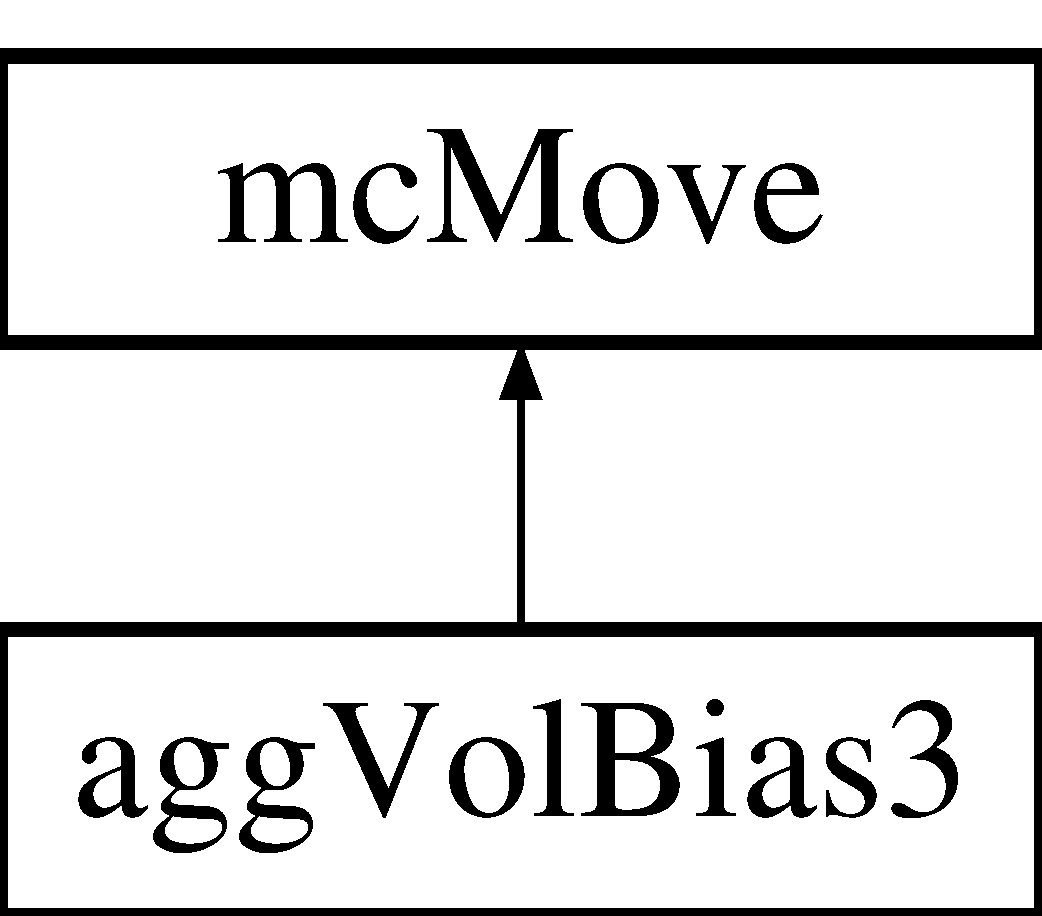
\includegraphics[height=2.000000cm]{classagg_vol_bias3}
\end{center}
\end{figure}
\subsection*{Public Member Functions}
\begin{DoxyCompactItemize}
\item 
\hyperlink{classagg_vol_bias3_a6fd174822857506eb4c61833ba6697ef}{agg\-Vol\-Bias3} ()
\item 
\hyperlink{classagg_vol_bias3_ac6a23cf87ba65eb6dba8f6512f0d7c78}{agg\-Vol\-Bias3} (const int type\-Index, const int type\-Index2, const double p\-Bias, const std\-::vector$<$ double $>$ rc1, const std\-::vector$<$ double $>$ rc2, const std\-::string tag)
\begin{DoxyCompactList}\small\item\em Instantiate a canonical aggregation-\/volume bias move to swap particles. \end{DoxyCompactList}\item 
int \hyperlink{classagg_vol_bias3_a59ebf724c8af1921045710fe9a08dd01}{make} (\hyperlink{classsim_system}{sim\-System} \&sys)
\begin{DoxyCompactList}\small\item\em Use aggregation-\/volume bias to swap two particles in the system. \end{DoxyCompactList}\end{DoxyCompactItemize}
\subsection*{Additional Inherited Members}


\subsection{Detailed Description}


Definition at line 11 of file aggvolbias.\-h.



\subsection{Constructor \& Destructor Documentation}
\hypertarget{classagg_vol_bias3_a6fd174822857506eb4c61833ba6697ef}{\index{agg\-Vol\-Bias3@{agg\-Vol\-Bias3}!agg\-Vol\-Bias3@{agg\-Vol\-Bias3}}
\index{agg\-Vol\-Bias3@{agg\-Vol\-Bias3}!aggVolBias3@{agg\-Vol\-Bias3}}
\subsubsection[{agg\-Vol\-Bias3}]{\setlength{\rightskip}{0pt plus 5cm}agg\-Vol\-Bias3\-::agg\-Vol\-Bias3 (
\begin{DoxyParamCaption}
{}
\end{DoxyParamCaption}
)\hspace{0.3cm}{\ttfamily [inline]}}}\label{classagg_vol_bias3_a6fd174822857506eb4c61833ba6697ef}


Definition at line 13 of file aggvolbias.\-h.



References mc\-Move\-::change\-N\-\_\-.


\begin{DoxyCode}
13 \{ \hyperlink{classmc_move_add8d6d08be181274a61c7463159ad929}{changeN\_} = \textcolor{keyword}{false}; pBias\_ = 0; \}
\end{DoxyCode}
\hypertarget{classagg_vol_bias3_ac6a23cf87ba65eb6dba8f6512f0d7c78}{\index{agg\-Vol\-Bias3@{agg\-Vol\-Bias3}!agg\-Vol\-Bias3@{agg\-Vol\-Bias3}}
\index{agg\-Vol\-Bias3@{agg\-Vol\-Bias3}!aggVolBias3@{agg\-Vol\-Bias3}}
\subsubsection[{agg\-Vol\-Bias3}]{\setlength{\rightskip}{0pt plus 5cm}agg\-Vol\-Bias3\-::agg\-Vol\-Bias3 (
\begin{DoxyParamCaption}
\item[{const int}]{type\-Index, }
\item[{const int}]{type\-Index2, }
\item[{const double}]{p\-Bias, }
\item[{const std\-::vector$<$ double $>$}]{rc1, }
\item[{const std\-::vector$<$ double $>$}]{rc2, }
\item[{const std\-::string}]{tag}
\end{DoxyParamCaption}
)}}\label{classagg_vol_bias3_ac6a23cf87ba65eb6dba8f6512f0d7c78}


Instantiate a canonical aggregation-\/volume bias move to swap particles. 

A\-V\-B\-M\-C3 from Chen and Siepmann, J. Phys. Chem. B 105 (2001).


\begin{DoxyParams}[1]{Parameters}
\mbox{\tt in}  & {\em type\-Index} & Type to consider in swapping in the vicinity of \\
\hline
\mbox{\tt in}  & {\em type\-Index2} & Second type to consider in swapping in the vicinity of \\
\hline
\mbox{\tt in}  & {\em p\-Bias} & Biasing probability \\
\hline
\mbox{\tt in}  & {\em rc1} & Radius (min, max) around particle of type\-Index to consider as being the \char`\"{}in\char`\"{} region \\
\hline
\mbox{\tt in}  & {\em rc2} & Radius (min, max) around particle of type\-Index2 to consider as being the \char`\"{}in\char`\"{} region \\
\hline
\mbox{\tt in}  & {\em tag} & Name modifier to identify move to user \\
\hline
\end{DoxyParams}


Definition at line 99 of file aggvolbias.\-cpp.



References mc\-Move\-::change\-N\-\_\-, mc\-Move\-::name\-\_\-, and mc\-Move\-::type\-Index\-\_\-.


\begin{DoxyCode}
99                                                                                                            
                                                                       \{
100     \hyperlink{classmc_move_acb731965547b0326ef318ec96da8b46a}{typeIndex\_} = typeIndex;
101     typeIndex2\_ = typeIndex2;
102 
103     \textcolor{keywordflow}{if} (pBias < 1 && pBias > 0) \{
104         pBias\_ = pBias;
105     \} \textcolor{keywordflow}{else} \{
106         \textcolor{keywordflow}{throw} \hyperlink{classcustom_exception}{customException} (\textcolor{stringliteral}{"Bias probability must be > 0 and < 1 for aggVolBias"});
107     \}
108 
109     \textcolor{keywordflow}{if} (!(rc1[0] > 0.0)) \{
110             \textcolor{keywordflow}{throw} \hyperlink{classcustom_exception}{customException} (\textcolor{stringliteral}{"Neighborhood radius for species 1 in aggVolBias must be
       > 0"});
111         \} \textcolor{keywordflow}{else} \{
112             rc1min\_ = rc1[0];
113         \}
114         \textcolor{keywordflow}{if} (!(rc2[0] > 0.0)) \{
115             \textcolor{keywordflow}{throw} \hyperlink{classcustom_exception}{customException} (\textcolor{stringliteral}{"Neighborhood radius for species 2 in aggVolBias must be
       > 0"});
116         \} \textcolor{keywordflow}{else} \{
117             rc2min\_ = rc2[0];
118         \}
119 
120     \textcolor{keywordflow}{if} (!(rc1[1] > rc1[0])) \{
121                 \textcolor{keywordflow}{throw} \hyperlink{classcustom_exception}{customException} (\textcolor{stringliteral}{"Max neighborhood radius for species 1 in aggVolBias
       must be > min"});
122         \} \textcolor{keywordflow}{else} \{
123                 rc1max\_ = rc1[1];
124         \}
125         \textcolor{keywordflow}{if} (!(rc2[1] > rc2[0])) \{
126                 \textcolor{keywordflow}{throw} \hyperlink{classcustom_exception}{customException} (\textcolor{stringliteral}{"Max neighborhood radius for species 2 in aggVolBias
       must be > min"});
127         \} \textcolor{keywordflow}{else} \{
128                 rc2max\_ = rc2[1];
129         \}
130 
131         \hyperlink{classmc_move_ac18c307855e1cb5751bd6e079857a8c5}{name\_} = tag + std::to\_string(typeIndex) + \textcolor{stringliteral}{"\_"} + std::to\_string(typeIndex2);
132     \hyperlink{classmc_move_add8d6d08be181274a61c7463159ad929}{changeN\_} = \textcolor{keyword}{false};
133 \}
\end{DoxyCode}


\subsection{Member Function Documentation}
\hypertarget{classagg_vol_bias3_a59ebf724c8af1921045710fe9a08dd01}{\index{agg\-Vol\-Bias3@{agg\-Vol\-Bias3}!make@{make}}
\index{make@{make}!aggVolBias3@{agg\-Vol\-Bias3}}
\subsubsection[{make}]{\setlength{\rightskip}{0pt plus 5cm}int agg\-Vol\-Bias3\-::make (
\begin{DoxyParamCaption}
\item[{{\bf sim\-System} \&}]{sys}
\end{DoxyParamCaption}
)\hspace{0.3cm}{\ttfamily [virtual]}}}\label{classagg_vol_bias3_a59ebf724c8af1921045710fe9a08dd01}


Use aggregation-\/volume bias to swap two particles in the system. 

All other information is stored in the \hyperlink{classsim_system}{sim\-System} object.


\begin{DoxyParams}[1]{Parameters}
\mbox{\tt in}  & {\em sys} & System object to attempt to swap particles in.\\
\hline
\end{DoxyParams}
\begin{DoxyReturn}{Returns}
M\-O\-V\-E\-\_\-\-S\-U\-C\-C\-E\-S\-S if particles are swapped, otherwise M\-O\-V\-E\-\_\-\-F\-A\-I\-L\-U\-R\-E if not. Will throw exceptions if there was an error. 
\end{DoxyReturn}


Implements \hyperlink{classmc_move_a2e377a628f9ecee5422fc8967d4924eb}{mc\-Move}.



Definition at line 142 of file aggvolbias.\-cpp.



References sim\-System\-::atoms, sim\-System\-::beta(), sim\-System\-::box(), calculate\-Bias(), sim\-System\-::get\-Current\-M(), sim\-System\-::get\-Fractional\-Atom\-Type(), sim\-System\-::get\-Tot\-N(), sim\-System\-::get\-W\-A\-L\-A\-Bias(), sim\-System\-::increment\-Energy(), M\-O\-V\-E\-\_\-\-F\-A\-I\-L\-U\-R\-E, M\-O\-V\-E\-\_\-\-S\-U\-C\-C\-E\-S\-S, sim\-System\-::n\-Species(), sim\-System\-::num\-Species, pbc\-Dist2(), P\-I, atom\-::pos, random3\-D\-Surface\-Vector(), rng(), R\-N\-G\-\_\-\-S\-E\-E\-D, sim\-System\-::tmmc\-Bias, sim\-System\-::translate\-Atom(), mc\-Move\-::type\-Index\-\_\-, wala\-::update(), tmmc\-::update\-C(), sim\-System\-::use\-T\-M\-M\-C, sim\-System\-::use\-W\-A\-L\-A, and custom\-Exception\-::what().


\begin{DoxyCode}
142                                      \{
143         \textcolor{comment}{// choose a particle of typeIndex\_}
144         \textcolor{keywordtype}{int} nAvail1 = sys.\hyperlink{classsim_system_a9eea865e6dc1cff377b1e79c4d9c23f0}{numSpecies}[\hyperlink{classmc_move_acb731965547b0326ef318ec96da8b46a}{typeIndex\_}];
145         \textcolor{keywordflow}{if} (sys.\hyperlink{classsim_system_a299fe4372e610b554eaaf5f5957b2dbc}{getCurrentM}() > 0 && sys.\hyperlink{classsim_system_a0500a9e84eecfbde7a98cf8a34f719d5}{getFractionalAtomType}() == 
      \hyperlink{classmc_move_acb731965547b0326ef318ec96da8b46a}{typeIndex\_}) \{
146             nAvail1++;
147         \}
148 
149         \textcolor{comment}{// choose a particle of typeIndex2\_}
150         \textcolor{keywordtype}{int} nAvail2 = sys.\hyperlink{classsim_system_a9eea865e6dc1cff377b1e79c4d9c23f0}{numSpecies}[typeIndex2\_];
151         \textcolor{keywordflow}{if} (sys.\hyperlink{classsim_system_a299fe4372e610b554eaaf5f5957b2dbc}{getCurrentM}() > 0 && sys.\hyperlink{classsim_system_a0500a9e84eecfbde7a98cf8a34f719d5}{getFractionalAtomType}() == 
      typeIndex2\_) \{
152             nAvail2++;
153         \}
154 
155         \textcolor{comment}{// update biases even upon failure to try move (also reject if types are same and only one overall
       particle)}
156         \textcolor{keywordflow}{if} (nAvail1 < 1 || nAvail2 < 1 || (\hyperlink{classmc_move_acb731965547b0326ef318ec96da8b46a}{typeIndex\_} == typeIndex2\_ && nAvail1 <= 1)) \{
157             \textcolor{keywordflow}{if} (sys.\hyperlink{classsim_system_aa83b00006b3919fb6e13f1bdeadece6a}{useWALA}) \{
158                     sys.\hyperlink{classsim_system_a7cb5049de8b0988349e89e30e4000407}{getWALABias}()->\hyperlink{classwala_ab439e3f60bea6c54522a870b9ad67acf}{update}(sys.\hyperlink{classsim_system_a37dd827f4057049763351510147b9f1d}{getTotN}(), sys.
      \hyperlink{classsim_system_a299fe4372e610b554eaaf5f5957b2dbc}{getCurrentM}());
159             \}
160             \textcolor{keywordflow}{if} (sys.\hyperlink{classsim_system_aa474a50b6353c8897331b1ab1ce53ab1}{useTMMC}) \{
161                     sys.\hyperlink{classsim_system_a13173f45a1e40a5f5a3552b0ebe15b54}{tmmcBias}->\hyperlink{classtmmc_ae067afc5b52af203b9d45f18d9737219}{updateC} (sys.\hyperlink{classsim_system_a37dd827f4057049763351510147b9f1d}{getTotN}(), sys.
      \hyperlink{classsim_system_a37dd827f4057049763351510147b9f1d}{getTotN}(), sys.\hyperlink{classsim_system_a299fe4372e610b554eaaf5f5957b2dbc}{getCurrentM}(), sys.\hyperlink{classsim_system_a299fe4372e610b554eaaf5f5957b2dbc}{getCurrentM}(), 0.0);
162             \}
163             \textcolor{keywordflow}{return} \hyperlink{moves_8h_a9832cf5fcfa8c0894545b591c9908e39}{MOVE\_FAILURE};
164         \}
165 
166         \textcolor{comment}{// choose particles, j and k - at present we are guaranteed at least 2 unique particles in the
       system}
167         \textcolor{keywordtype}{int} pkJ = (int) floor(\hyperlink{utilities_8cpp_a0f9542af4b475ac79cb679d7a8d14db0}{rng} (&\hyperlink{global_8h_a3f4e4ea24d5a5c66feae55d1f329c884}{RNG\_SEED}) * nAvail1), pkK = 0, iterMax = 25, iter = 0;
168         \textcolor{keywordtype}{bool} jkOverlap = \textcolor{keyword}{true};
169         \textcolor{keywordflow}{while} (jkOverlap && iter < iterMax) \{
170             \textcolor{comment}{// if there are only a few particles in the system, they may all overlap so reject after a
       number of trials}
171             iter++;
172 
173             pkK = (int) floor(\hyperlink{utilities_8cpp_a0f9542af4b475ac79cb679d7a8d14db0}{rng} (&\hyperlink{global_8h_a3f4e4ea24d5a5c66feae55d1f329c884}{RNG\_SEED}) * nAvail2);
174 
175             \textcolor{comment}{// establish if j and k overlap their "in" regions}
176             \textcolor{keyword}{const} \textcolor{keywordtype}{double} rc = (rc1max\_ + rc2max\_)/2.0;
177 
178             \textcolor{comment}{// if pkK and pkJ are withing rcut of each other, they overlap}
179             \textcolor{keywordflow}{if} (\hyperlink{utilities_8cpp_abb1db3a8a3ac46e044bbe7b2c5684c0a}{pbcDist2}(sys.\hyperlink{classsim_system_a90421b19082f7fb8fc23b7264b1161e4}{atoms}[\hyperlink{classmc_move_acb731965547b0326ef318ec96da8b46a}{typeIndex\_}][pkJ].pos, sys.
      \hyperlink{classsim_system_a90421b19082f7fb8fc23b7264b1161e4}{atoms}[typeIndex2\_][pkK].pos, sys.\hyperlink{classsim_system_a8bff9dfb95b1b09a0fab2c1c485ade07}{box}()) > rc*rc) \{
180                     jkOverlap = \textcolor{keyword}{false};
181             \}
182 
183             \textcolor{comment}{// However, we also technically need to ensure that if typeIndex\_ == typeIndex2\_, j and k are
       not the same particle.}
184             \textcolor{comment}{// Happily, this is already guaranteed by the above distance check (a particle is a distance 0
       from itself)}
185         \}
186 
187         \textcolor{comment}{// check for failure to find pkJ and pkK}
188         \textcolor{keywordflow}{if} (iter >= iterMax) \{
189             \textcolor{keywordflow}{if} (sys.\hyperlink{classsim_system_aa83b00006b3919fb6e13f1bdeadece6a}{useWALA}) \{
190                     sys.\hyperlink{classsim_system_a7cb5049de8b0988349e89e30e4000407}{getWALABias}()->\hyperlink{classwala_ab439e3f60bea6c54522a870b9ad67acf}{update}(sys.\hyperlink{classsim_system_a37dd827f4057049763351510147b9f1d}{getTotN}(), sys.
      \hyperlink{classsim_system_a299fe4372e610b554eaaf5f5957b2dbc}{getCurrentM}());
191             \}
192             \textcolor{keywordflow}{if} (sys.\hyperlink{classsim_system_aa474a50b6353c8897331b1ab1ce53ab1}{useTMMC}) \{
193                     sys.\hyperlink{classsim_system_a13173f45a1e40a5f5a3552b0ebe15b54}{tmmcBias}->\hyperlink{classtmmc_ae067afc5b52af203b9d45f18d9737219}{updateC} (sys.\hyperlink{classsim_system_a37dd827f4057049763351510147b9f1d}{getTotN}(), sys.
      \hyperlink{classsim_system_a37dd827f4057049763351510147b9f1d}{getTotN}(), sys.\hyperlink{classsim_system_a299fe4372e610b554eaaf5f5957b2dbc}{getCurrentM}(), sys.\hyperlink{classsim_system_a299fe4372e610b554eaaf5f5957b2dbc}{getCurrentM}(), 0.0);
194             \}
195             \textcolor{keywordflow}{return} \hyperlink{moves_8h_a9832cf5fcfa8c0894545b591c9908e39}{MOVE\_FAILURE};
196         \}
197 
198         \textcolor{keyword}{const} std::vector < double > box = sys.\hyperlink{classsim_system_a8bff9dfb95b1b09a0fab2c1c485ade07}{box}();
199         \textcolor{keywordtype}{double} minL = box[0];
200         \textcolor{keywordtype}{double} V = 1.0;
201         \textcolor{keywordflow}{for} (\textcolor{keywordtype}{unsigned} \textcolor{keywordtype}{int} i = 0; i < box.size(); ++i) \{
202             V *= box[i];
203             minL = std::min(minL, box[i]);
204         \}
205 
206         \textcolor{comment}{// sanity check for rc's}
207         \textcolor{keywordflow}{if} (!(rc1max\_ < minL/2.0)) \{
208             \textcolor{keywordflow}{throw} \hyperlink{classcustom_exception}{customException} (\textcolor{stringliteral}{"Max neighborhood radius for species 1 in aggVolBias must
       be < box/2"});
209         \}
210         \textcolor{keywordflow}{if} (!(rc2max\_ < minL/2.0)) \{
211             \textcolor{keywordflow}{throw} \hyperlink{classcustom_exception}{customException} (\textcolor{stringliteral}{"Max neighborhood radius for species 2 in aggVolBias must
       be < box/2"});
212         \}
213 
214         \textcolor{comment}{// based on the choices made below, the unbiased acceptance probability will be set in each case}
215         \textcolor{keywordtype}{double} p\_u = 1.0, bias = 1.0, dU = 0.0;
216     \textcolor{keywordtype}{double} V\_in\_j = 0.0, V\_in\_k = 0.0, V\_out\_j = 0.0, V\_out\_k = 0.0;
217         \textcolor{keywordtype}{int} chosenAtomType = 0;
218     \textcolor{keywordtype}{int}  N\_in\_k = 0, N\_in\_j = 0, N\_out\_k = 0, N\_out\_j = 0;
219         \hyperlink{classatom}{atom}* chosenAtom;
220         \hyperlink{classatom}{atom} tmpNewAtom; \textcolor{comment}{// stores position the chosenAtom is being proposed to be moved to}
221         \textcolor{keywordtype}{bool} inA = \textcolor{keyword}{false}; \textcolor{comment}{// is this a "in" to X move?}
222 
223         \textcolor{keywordflow}{if} (\hyperlink{utilities_8cpp_a0f9542af4b475ac79cb679d7a8d14db0}{rng}(&\hyperlink{global_8h_a3f4e4ea24d5a5c66feae55d1f329c884}{RNG\_SEED}) < pBias\_) \{
224             \textcolor{comment}{// choose a particle either "in" k or "out" j with equal probability}
225             \textcolor{comment}{// note that "out" j includes the "in" k region as well}
226             \textcolor{keywordflow}{if} (\hyperlink{utilities_8cpp_a0f9542af4b475ac79cb679d7a8d14db0}{rng} (&\hyperlink{global_8h_a3f4e4ea24d5a5c66feae55d1f329c884}{RNG\_SEED}) < 0.5) \{
227                     \textcolor{comment}{// choose particle "in" k, this chosen particle can be of any type}
228                     inA = \textcolor{keyword}{true};
229             std::vector < atom* > neighborAtoms;
230                     neighborAtoms.reserve(100); \textcolor{comment}{// 100 is just an arbitrary number to help accelerate}
231                     std::vector < int > nEachType (sys.\hyperlink{classsim_system_ab5e2e9b6204de15520302fe1d51688dd}{nSpecies}(), 0);
232                     \textcolor{keywordflow}{for} (\textcolor{keywordtype}{unsigned} \textcolor{keywordtype}{int} i = 0; i < sys.\hyperlink{classsim_system_ab5e2e9b6204de15520302fe1d51688dd}{nSpecies}(); ++i) \{
233                         \textcolor{keywordtype}{int} totKatoms = sys.\hyperlink{classsim_system_a9eea865e6dc1cff377b1e79c4d9c23f0}{numSpecies}[i];
234 
235                         \textcolor{comment}{// account for if in expanded ensemble and have an additional partially inserted
       particle floating around}
236                         \textcolor{keywordflow}{if} (sys.\hyperlink{classsim_system_a299fe4372e610b554eaaf5f5957b2dbc}{getCurrentM}() > 0 && sys.
      \hyperlink{classsim_system_a0500a9e84eecfbde7a98cf8a34f719d5}{getFractionalAtomType}() == i) \{
237                                 totKatoms++;
238                         \}
239 
240                         \textcolor{keywordflow}{for} (\textcolor{keywordtype}{unsigned} \textcolor{keywordtype}{int} j = 0; j < totKatoms; ++j) \{
241                     \textcolor{keyword}{const} \textcolor{keywordtype}{double} d2 = \hyperlink{utilities_8cpp_abb1db3a8a3ac46e044bbe7b2c5684c0a}{pbcDist2}(sys.\hyperlink{classsim_system_a90421b19082f7fb8fc23b7264b1161e4}{atoms}[i][j].pos, sys.
      \hyperlink{classsim_system_a90421b19082f7fb8fc23b7264b1161e4}{atoms}[typeIndex2\_][pkK].pos, sys.\hyperlink{classsim_system_a8bff9dfb95b1b09a0fab2c1c485ade07}{box}());
242                                 \textcolor{keywordflow}{if} (d2 < rc2max\_*rc2max\_ && d2 >= rc2min\_*rc2min\_) \{
243                                     \textcolor{keywordflow}{if} (&sys.\hyperlink{classsim_system_a90421b19082f7fb8fc23b7264b1161e4}{atoms}[typeIndex2\_][pkK] != &sys.
      \hyperlink{classsim_system_a90421b19082f7fb8fc23b7264b1161e4}{atoms}[i][j]) \{ \textcolor{comment}{// since J and K do not overlap do not have to check if this is pkJ}
244                                             neighborAtoms.push\_back(&sys.\hyperlink{classsim_system_a90421b19082f7fb8fc23b7264b1161e4}{atoms}[i][j]);
245                                             nEachType[i] += 1;
246                                     \}
247                                 \}
248                         \}
249                     \}
250 
251                     \textcolor{comment}{// reject move if no neighbors}
252                     \textcolor{keywordflow}{if} (neighborAtoms.begin() == neighborAtoms.end()) \{
253                         \textcolor{keywordflow}{if} (sys.\hyperlink{classsim_system_aa83b00006b3919fb6e13f1bdeadece6a}{useWALA}) \{
254                                 sys.\hyperlink{classsim_system_a7cb5049de8b0988349e89e30e4000407}{getWALABias}()->\hyperlink{classwala_ab439e3f60bea6c54522a870b9ad67acf}{update}(sys.
      \hyperlink{classsim_system_a37dd827f4057049763351510147b9f1d}{getTotN}(), sys.\hyperlink{classsim_system_a299fe4372e610b554eaaf5f5957b2dbc}{getCurrentM}());
255                         \}
256                         \textcolor{keywordflow}{if} (sys.\hyperlink{classsim_system_aa474a50b6353c8897331b1ab1ce53ab1}{useTMMC}) \{
257                                 sys.\hyperlink{classsim_system_a13173f45a1e40a5f5a3552b0ebe15b54}{tmmcBias}->\hyperlink{classtmmc_ae067afc5b52af203b9d45f18d9737219}{updateC} (sys.
      \hyperlink{classsim_system_a37dd827f4057049763351510147b9f1d}{getTotN}(), sys.\hyperlink{classsim_system_a37dd827f4057049763351510147b9f1d}{getTotN}(), sys.\hyperlink{classsim_system_a299fe4372e610b554eaaf5f5957b2dbc}{getCurrentM}(), sys.
      \hyperlink{classsim_system_a299fe4372e610b554eaaf5f5957b2dbc}{getCurrentM}(), 0.0);
258                         \}
259                         \textcolor{keywordflow}{return} \hyperlink{moves_8h_a9832cf5fcfa8c0894545b591c9908e39}{MOVE\_FAILURE};
260                     \}
261 
262                     \textcolor{comment}{// otherwise choose an atom}
263                     \textcolor{keyword}{const} \textcolor{keywordtype}{int} atomIndex = (int) floor(\hyperlink{utilities_8cpp_a0f9542af4b475ac79cb679d7a8d14db0}{rng} (&\hyperlink{global_8h_a3f4e4ea24d5a5c66feae55d1f329c884}{RNG\_SEED}) * neighborAtoms.size());
264                     chosenAtom = neighborAtoms[atomIndex];
265                 \textcolor{keywordtype}{int} tot = 0;
266                     \textcolor{keywordflow}{while} (tot < atomIndex) \{
267                         tot += nEachType[chosenAtomType];
268                         chosenAtomType++;
269                         \textcolor{keywordflow}{if} (chosenAtomType > sys.\hyperlink{classsim_system_ab5e2e9b6204de15520302fe1d51688dd}{nSpecies}()) \{ \textcolor{comment}{// > not >= because chosenAtomType
       will be decremented next}
270                                 \textcolor{keywordflow}{throw} \hyperlink{classcustom_exception}{customException} (\textcolor{stringliteral}{"Error, could not properly identify
       the type of the atom chosen to be moved in aggVolBias"});
271                         \}
272                     \}
273                     chosenAtomType--;
274                     \textcolor{keywordflow}{if} (chosenAtomType < 0) \{ \textcolor{comment}{// in case atomIndex = 0 and above loop did not execute at
       all}
275                         chosenAtomType = 0;
276                     \}
277 
278             N\_in\_k = nEachType[chosenAtomType]; \textcolor{comment}{// only concerned about the number of the chosen type}
279             V\_in\_k = 4.0/3.0*\hyperlink{global_8h_a598a3330b3c21701223ee0ca14316eca}{PI}*(rc2max\_*rc2max\_*rc2max\_ - rc2min\_*rc2min\_*rc2min\_);
280         \} \textcolor{keywordflow}{else} \{
281                     \textcolor{comment}{// choose particle "out" of j, this chosen particle can be of any type}
282                     inA = \textcolor{keyword}{false};
283 
284                     \textcolor{comment}{// just pick atoms (of any type) at random and see if it is "out" of j}
285                     \textcolor{comment}{// this should be faster than establishing, a priori, all atoms which are "out"}
286                     \textcolor{comment}{// and then picking from that list since *most* atoms should be "out"}
287                     \textcolor{comment}{// unlike when we have to pick from "in" ones which are more rare}
288 
289             \textcolor{keywordtype}{int} iter = 0, iterMax = 25;
290                     \textcolor{keywordtype}{bool} inJ = \textcolor{keyword}{true};
291 
292             \textcolor{keywordflow}{while} (inJ && iter < iterMax) \{
293                         iter++;
294                         \textcolor{keyword}{const} \textcolor{keywordtype}{int} ranSpec = (int) floor(\hyperlink{utilities_8cpp_a0f9542af4b475ac79cb679d7a8d14db0}{rng} (&\hyperlink{global_8h_a3f4e4ea24d5a5c66feae55d1f329c884}{RNG\_SEED}) * sys.
      \hyperlink{classsim_system_ab5e2e9b6204de15520302fe1d51688dd}{nSpecies}());
295                         \textcolor{keywordtype}{int} availAtoms = sys.\hyperlink{classsim_system_a9eea865e6dc1cff377b1e79c4d9c23f0}{numSpecies}[ranSpec];
296                         \textcolor{comment}{// account for if in expanded ensemble and have an additional partially inserted
       particle floating around}
297                         \textcolor{keywordflow}{if} (sys.\hyperlink{classsim_system_a299fe4372e610b554eaaf5f5957b2dbc}{getCurrentM}() > 0 && sys.
      \hyperlink{classsim_system_a0500a9e84eecfbde7a98cf8a34f719d5}{getFractionalAtomType}() == ranSpec) \{
298                             availAtoms++;
299                         \}
300                         \textcolor{keywordtype}{int} ranIndex = (int) floor(\hyperlink{utilities_8cpp_a0f9542af4b475ac79cb679d7a8d14db0}{rng} (&\hyperlink{global_8h_a3f4e4ea24d5a5c66feae55d1f329c884}{RNG\_SEED}) * availAtoms);
301 
302                         \textcolor{comment}{// check this atom is neither pkJ nor pkK}
303                         \textcolor{keywordflow}{if} (&sys.\hyperlink{classsim_system_a90421b19082f7fb8fc23b7264b1161e4}{atoms}[ranSpec][ranIndex] != &sys.\hyperlink{classsim_system_a90421b19082f7fb8fc23b7264b1161e4}{atoms}[
      \hyperlink{classmc_move_acb731965547b0326ef318ec96da8b46a}{typeIndex\_}][pkJ] && &sys.\hyperlink{classsim_system_a90421b19082f7fb8fc23b7264b1161e4}{atoms}[ranSpec][ranIndex] != &sys.\hyperlink{classsim_system_a90421b19082f7fb8fc23b7264b1161e4}{atoms}[typeIndex2\_][pkK]) \{
304                             \textcolor{keyword}{const} \textcolor{keywordtype}{double} d2 = \hyperlink{utilities_8cpp_abb1db3a8a3ac46e044bbe7b2c5684c0a}{pbcDist2}(sys.\hyperlink{classsim_system_a90421b19082f7fb8fc23b7264b1161e4}{atoms}[ranSpec][ranIndex].pos, sys.
      \hyperlink{classsim_system_a90421b19082f7fb8fc23b7264b1161e4}{atoms}[\hyperlink{classmc_move_acb731965547b0326ef318ec96da8b46a}{typeIndex\_}][pkJ].pos, sys.\hyperlink{classsim_system_a8bff9dfb95b1b09a0fab2c1c485ade07}{box}());
305                     \textcolor{keywordflow}{if} (!(d2 < rc1max\_*rc1max\_ && d2 >= rc1min\_*rc1min\_)) \{
306                                     chosenAtom = &sys.\hyperlink{classsim_system_a90421b19082f7fb8fc23b7264b1161e4}{atoms}[ranSpec][ranIndex];
307                                     chosenAtomType = ranSpec;
308                                     inJ = \textcolor{keyword}{false};
309                                 \}
310                         \}
311                     \}
312 
313                     \textcolor{comment}{// check if we could not locate a particle "out" of j}
314                     \textcolor{keywordflow}{if} (iter >= iterMax) \{
315                         \textcolor{keywordflow}{if} (sys.\hyperlink{classsim_system_aa83b00006b3919fb6e13f1bdeadece6a}{useWALA}) \{
316                                 sys.\hyperlink{classsim_system_a7cb5049de8b0988349e89e30e4000407}{getWALABias}()->\hyperlink{classwala_ab439e3f60bea6c54522a870b9ad67acf}{update}(sys.
      \hyperlink{classsim_system_a37dd827f4057049763351510147b9f1d}{getTotN}(), sys.\hyperlink{classsim_system_a299fe4372e610b554eaaf5f5957b2dbc}{getCurrentM}());
317                         \}
318                         \textcolor{keywordflow}{if} (sys.\hyperlink{classsim_system_aa474a50b6353c8897331b1ab1ce53ab1}{useTMMC}) \{
319                                 sys.\hyperlink{classsim_system_a13173f45a1e40a5f5a3552b0ebe15b54}{tmmcBias}->\hyperlink{classtmmc_ae067afc5b52af203b9d45f18d9737219}{updateC} (sys.
      \hyperlink{classsim_system_a37dd827f4057049763351510147b9f1d}{getTotN}(), sys.\hyperlink{classsim_system_a37dd827f4057049763351510147b9f1d}{getTotN}(), sys.\hyperlink{classsim_system_a299fe4372e610b554eaaf5f5957b2dbc}{getCurrentM}(), sys.
      \hyperlink{classsim_system_a299fe4372e610b554eaaf5f5957b2dbc}{getCurrentM}(), 0.0);
320                         \}
321                         \textcolor{keywordflow}{return} \hyperlink{moves_8h_a9832cf5fcfa8c0894545b591c9908e39}{MOVE\_FAILURE};
322                     \}
323 
324             \textcolor{comment}{// need to know how many chosenAtoms are "out" of j}
325             \textcolor{keywordtype}{int} totJatoms = sys.\hyperlink{classsim_system_a9eea865e6dc1cff377b1e79c4d9c23f0}{numSpecies}[chosenAtomType];
326 
327                 \textcolor{comment}{// account for if in expanded ensemble and have an additional partially inserted particle
       floating around}
328                 \textcolor{keywordflow}{if} (sys.\hyperlink{classsim_system_a299fe4372e610b554eaaf5f5957b2dbc}{getCurrentM}() > 0 && sys.
      \hyperlink{classsim_system_a0500a9e84eecfbde7a98cf8a34f719d5}{getFractionalAtomType}() == chosenAtomType) \{
329                         totJatoms++;
330                 \}
331 
332             \textcolor{comment}{// need for V\_out\_j later}
333             V\_in\_k = 4.0/3.0*\hyperlink{global_8h_a598a3330b3c21701223ee0ca14316eca}{PI}*(rc2max\_*rc2max\_*rc2max\_ - rc2min\_*rc2min\_*rc2min\_);
334             \}
335 
336             \textcolor{comment}{// move the chosenAtom "in" j}
337 
338             \textcolor{comment}{// (1) get energy of chosenAtom in current state}
339             \textcolor{keywordtype}{double} oldEnergy = 0.0;
340             \textcolor{keywordflow}{try} \{
341                 oldEnergy = getTempEnergy\_ (sys, box, V, chosenAtomType, chosenAtom);
342             \} \textcolor{keywordflow}{catch} (\hyperlink{classcustom_exception}{customException} &ce) \{
343                     \textcolor{keywordflow}{throw} \hyperlink{classcustom_exception}{customException} (ce.\hyperlink{classcustom_exception_aeb6ab5848b038adfc68fde86a512f691}{what}());
344             \}
345 
346             \textcolor{comment}{// (2) "move" chosenAtom - randomly choose a radius from [0, rc1) around pkJ}
347             \textcolor{keyword}{const} \textcolor{keywordtype}{double} dr = (rc1max\_ - rc1min\_);
348         \textcolor{keyword}{const} \textcolor{keywordtype}{double} magnitude = pow((\hyperlink{utilities_8cpp_a0f9542af4b475ac79cb679d7a8d14db0}{rng} (&\hyperlink{global_8h_a3f4e4ea24d5a5c66feae55d1f329c884}{RNG\_SEED})*dr*dr*dr+rc1min\_*rc1min\_*rc1min\_), 1./3.);
349 
350             \textcolor{comment}{// then choose a point randomly on the surface of that sphere to place chosenAtom}
351             std::vector < double > surfaceVec = \hyperlink{utilities_8cpp_af1bc480936b7436d4e679abc5a837815}{random3DSurfaceVector} (magnitude), 
      origPos = chosenAtom->\hyperlink{classatom_a3ae5f4880e7831d8b2c9fda72b4eb24a}{pos};
352             \textcolor{keywordflow}{for} (\textcolor{keywordtype}{unsigned} \textcolor{keywordtype}{int} i = 0; i < origPos.size(); ++i) \{
353                 chosenAtom->\hyperlink{classatom_a3ae5f4880e7831d8b2c9fda72b4eb24a}{pos}[i] = sys.\hyperlink{classsim_system_a90421b19082f7fb8fc23b7264b1161e4}{atoms}[\hyperlink{classmc_move_acb731965547b0326ef318ec96da8b46a}{typeIndex\_}][pkJ].pos[i] + surfaceVec[i];
354 
355                 \textcolor{comment}{// apply periodic boundary conditions}
356                 \textcolor{keywordflow}{if} (chosenAtom->\hyperlink{classatom_a3ae5f4880e7831d8b2c9fda72b4eb24a}{pos}[i] >= box[i]) \{
357                         chosenAtom->\hyperlink{classatom_a3ae5f4880e7831d8b2c9fda72b4eb24a}{pos}[i] -= box[i];
358                     \} \textcolor{keywordflow}{else} \textcolor{keywordflow}{if} (chosenAtom->\hyperlink{classatom_a3ae5f4880e7831d8b2c9fda72b4eb24a}{pos}[i] < 0) \{
359                         chosenAtom->\hyperlink{classatom_a3ae5f4880e7831d8b2c9fda72b4eb24a}{pos}[i] += box[i];
360                     \}
361             \}
362 
363             \textcolor{comment}{// store the newly proposed position for later}
364             tmpNewAtom.\hyperlink{classatom_a3ae5f4880e7831d8b2c9fda72b4eb24a}{pos} = chosenAtom->\hyperlink{classatom_a3ae5f4880e7831d8b2c9fda72b4eb24a}{pos};
365 
366         \textcolor{comment}{// establish how many chosenAtoms are "in" j}
367         \textcolor{keywordtype}{int} totJatoms = sys.\hyperlink{classsim_system_a9eea865e6dc1cff377b1e79c4d9c23f0}{numSpecies}[chosenAtomType];
368 
369             \textcolor{comment}{// account for if in expanded ensemble and have an additional partially inserted particle
       floating around}
370             \textcolor{keywordflow}{if} (sys.\hyperlink{classsim_system_a299fe4372e610b554eaaf5f5957b2dbc}{getCurrentM}() > 0 && sys.\hyperlink{classsim_system_a0500a9e84eecfbde7a98cf8a34f719d5}{getFractionalAtomType}() == 
      chosenAtomType) \{
371                 totJatoms++;
372             \}
373 
374         N\_in\_j = 0;
375             \textcolor{keywordflow}{for} (\textcolor{keywordtype}{unsigned} \textcolor{keywordtype}{int} j = 0; j < totJatoms; ++j) \{
376                 \textcolor{keyword}{const} \textcolor{keywordtype}{double} d2 = \hyperlink{utilities_8cpp_abb1db3a8a3ac46e044bbe7b2c5684c0a}{pbcDist2}(sys.\hyperlink{classsim_system_a90421b19082f7fb8fc23b7264b1161e4}{atoms}[chosenAtomType][j].pos, sys.
      \hyperlink{classsim_system_a90421b19082f7fb8fc23b7264b1161e4}{atoms}[\hyperlink{classmc_move_acb731965547b0326ef318ec96da8b46a}{typeIndex\_}][pkJ].pos, sys.\hyperlink{classsim_system_a8bff9dfb95b1b09a0fab2c1c485ade07}{box}());
377             \textcolor{keywordflow}{if} (d2 < rc1max\_*rc1max\_ && d2 >= rc1min\_*rc1min\_) \{
378                             \textcolor{keywordflow}{if} (&sys.\hyperlink{classsim_system_a90421b19082f7fb8fc23b7264b1161e4}{atoms}[chosenAtomType][j] != &sys.\hyperlink{classsim_system_a90421b19082f7fb8fc23b7264b1161e4}{atoms}[
      \hyperlink{classmc_move_acb731965547b0326ef318ec96da8b46a}{typeIndex\_}][pkJ]) \{
379                     N\_in\_j++;
380                 \}
381             \}
382         \}
383 
384 
385         N\_out\_j = totJatoms - N\_in\_j;
386         V\_in\_j = 4.0/3.0*\hyperlink{global_8h_a598a3330b3c21701223ee0ca14316eca}{PI}*(rc1max\_*rc1max\_*rc1max\_ - rc1min\_*rc1min\_*rc1min\_);
387 
388             \textcolor{keywordtype}{double} newEnergy = 0.0;
389             \textcolor{keywordflow}{try} \{
390                 newEnergy = getTempEnergy\_ (sys, box, V, chosenAtomType, chosenAtom);
391             \} \textcolor{keywordflow}{catch} (\hyperlink{classcustom_exception}{customException} &ce) \{
392                 \textcolor{keywordflow}{throw} \hyperlink{classcustom_exception}{customException} (ce.\hyperlink{classcustom_exception_aeb6ab5848b038adfc68fde86a512f691}{what}());
393             \}
394 
395             \textcolor{comment}{// restore the atom's original state before continuing}
396             chosenAtom->\hyperlink{classatom_a3ae5f4880e7831d8b2c9fda72b4eb24a}{pos} = origPos;
397 
398             \textcolor{comment}{// assign p\_u}
399             dU = newEnergy - oldEnergy;
400             p\_u =  0.0;
401         \textcolor{keywordflow}{if} (inA) \{
402             \textcolor{comment}{// "in K" to "in J" move}
403             p\_u = (1.0 - pBias\_)*V\_in\_j*N\_in\_k*exp(-dU*sys.\hyperlink{classsim_system_a3eeec9678902f8d7fce4dad6064aaf4c}{beta}())/(pBias\_*V\_in\_k*(N\_in\_j+1.0));
404         \} \textcolor{keywordflow}{else} \{
405             \textcolor{comment}{// "out J" to "in J" move}
406             V\_out\_j = V - V\_in\_j - V\_in\_k; \textcolor{comment}{// V\_in\_k subtracted must also be done consistently}
407             p\_u = (1.0 - pBias\_)*V\_in\_j*N\_out\_j*exp(-dU*sys.\hyperlink{classsim_system_a3eeec9678902f8d7fce4dad6064aaf4c}{beta}())/((1.0 - pBias\_)*V\_out\_j*(N\_in\_j + 1
      .0));
408         \}
409     \} \textcolor{keywordflow}{else} \{
410         \textcolor{comment}{// choose a particle "in" j, this chosen particle can be of any type}
411             std::vector < atom* > neighborAtoms;
412             neighborAtoms.reserve(100); \textcolor{comment}{// 100 is just an arbitrary number to help accelerate}
413             std::vector < int > nEachType (sys.\hyperlink{classsim_system_ab5e2e9b6204de15520302fe1d51688dd}{nSpecies}(), 0);
414         \textcolor{keywordflow}{for} (\textcolor{keywordtype}{unsigned} \textcolor{keywordtype}{int} i = 0; i < sys.\hyperlink{classsim_system_ab5e2e9b6204de15520302fe1d51688dd}{nSpecies}(); ++i) \{
415                     \textcolor{keywordtype}{int} totJatoms = sys.\hyperlink{classsim_system_a9eea865e6dc1cff377b1e79c4d9c23f0}{numSpecies}[i];
416 
417                     \textcolor{comment}{// account for if in expanded ensemble and have an additional partially inserted
       particle floating around}
418                     \textcolor{keywordflow}{if} (sys.\hyperlink{classsim_system_a299fe4372e610b554eaaf5f5957b2dbc}{getCurrentM}() > 0 && sys.
      \hyperlink{classsim_system_a0500a9e84eecfbde7a98cf8a34f719d5}{getFractionalAtomType}() == i) \{
419                         totJatoms++;
420                     \}
421 
422                     \textcolor{keywordflow}{for} (\textcolor{keywordtype}{unsigned} \textcolor{keywordtype}{int} j = 0; j < totJatoms; ++j) \{
423                         \textcolor{keyword}{const} \textcolor{keywordtype}{double} d2 = \hyperlink{utilities_8cpp_abb1db3a8a3ac46e044bbe7b2c5684c0a}{pbcDist2}(sys.\hyperlink{classsim_system_a90421b19082f7fb8fc23b7264b1161e4}{atoms}[i][j].pos, sys.
      \hyperlink{classsim_system_a90421b19082f7fb8fc23b7264b1161e4}{atoms}[\hyperlink{classmc_move_acb731965547b0326ef318ec96da8b46a}{typeIndex\_}][pkJ].pos, sys.\hyperlink{classsim_system_a8bff9dfb95b1b09a0fab2c1c485ade07}{box}());
424                 \textcolor{keywordflow}{if} (d2 < rc1max\_*rc1max\_ && d2 >= rc1min\_*rc1min\_) \{
425                                 \textcolor{keywordflow}{if} (&sys.\hyperlink{classsim_system_a90421b19082f7fb8fc23b7264b1161e4}{atoms}[\hyperlink{classmc_move_acb731965547b0326ef318ec96da8b46a}{typeIndex\_}][pkJ] != &sys.
      \hyperlink{classsim_system_a90421b19082f7fb8fc23b7264b1161e4}{atoms}[i][j]) \{ \textcolor{comment}{// since J and K do not overlap do not have to check this is pkK}
426                                     neighborAtoms.push\_back(&sys.\hyperlink{classsim_system_a90421b19082f7fb8fc23b7264b1161e4}{atoms}[i][j]);
427                                     nEachType[i] += 1;
428                             \}
429                         \}
430                     \}
431             \}
432 
433             \textcolor{comment}{// reject move if no neighbors}
434             \textcolor{keywordflow}{if} (neighborAtoms.begin() == neighborAtoms.end()) \{
435                 \textcolor{keywordflow}{if} (sys.\hyperlink{classsim_system_aa83b00006b3919fb6e13f1bdeadece6a}{useWALA}) \{
436                         sys.\hyperlink{classsim_system_a7cb5049de8b0988349e89e30e4000407}{getWALABias}()->\hyperlink{classwala_ab439e3f60bea6c54522a870b9ad67acf}{update}(sys.\hyperlink{classsim_system_a37dd827f4057049763351510147b9f1d}{getTotN}(), sys.
      \hyperlink{classsim_system_a299fe4372e610b554eaaf5f5957b2dbc}{getCurrentM}());
437                     \}
438                     \textcolor{keywordflow}{if} (sys.\hyperlink{classsim_system_aa474a50b6353c8897331b1ab1ce53ab1}{useTMMC}) \{
439                         sys.\hyperlink{classsim_system_a13173f45a1e40a5f5a3552b0ebe15b54}{tmmcBias}->\hyperlink{classtmmc_ae067afc5b52af203b9d45f18d9737219}{updateC} (sys.\hyperlink{classsim_system_a37dd827f4057049763351510147b9f1d}{getTotN}(), sys.
      \hyperlink{classsim_system_a37dd827f4057049763351510147b9f1d}{getTotN}(), sys.\hyperlink{classsim_system_a299fe4372e610b554eaaf5f5957b2dbc}{getCurrentM}(), sys.\hyperlink{classsim_system_a299fe4372e610b554eaaf5f5957b2dbc}{getCurrentM}(), 0.0);
440                     \}
441                 \textcolor{keywordflow}{return} \hyperlink{moves_8h_a9832cf5fcfa8c0894545b591c9908e39}{MOVE\_FAILURE};
442             \}
443 
444             \textcolor{comment}{// otherwise choose an atom}
445             \textcolor{keyword}{const} \textcolor{keywordtype}{int} atomIndex = (int) floor(\hyperlink{utilities_8cpp_a0f9542af4b475ac79cb679d7a8d14db0}{rng} (&\hyperlink{global_8h_a3f4e4ea24d5a5c66feae55d1f329c884}{RNG\_SEED}) * neighborAtoms.size());
446             chosenAtom = neighborAtoms[atomIndex];
447         \textcolor{keywordtype}{int} tot = 0;
448             \textcolor{keywordflow}{while} (tot < atomIndex) \{
449                 tot += nEachType[chosenAtomType];
450                 chosenAtomType++;
451                     \textcolor{keywordflow}{if} (chosenAtomType > sys.\hyperlink{classsim_system_ab5e2e9b6204de15520302fe1d51688dd}{nSpecies}()) \{ \textcolor{comment}{// > not >= because chosenAtomType will
       be decremented next}
452                         \textcolor{keywordflow}{throw} \hyperlink{classcustom_exception}{customException} (\textcolor{stringliteral}{"Error, could not properly identify the type
       of the atom chosen to be moved in aggVolBias"});
453                     \}
454             \}
455             chosenAtomType--;
456             \textcolor{keywordflow}{if} (chosenAtomType < 0) \{ \textcolor{comment}{// in case atomIndex = 0 and above loop did not execute at all}
457                     chosenAtomType = 0;
458             \}
459 
460         N\_in\_j = nEachType[chosenAtomType];
461         V\_in\_j = 4.0/3.0*\hyperlink{global_8h_a598a3330b3c21701223ee0ca14316eca}{PI}*(rc1max\_*rc1max\_*rc1max\_ - rc1min\_*rc1min\_*rc1min\_);
462 
463         \textcolor{comment}{// what to do with chosenAtom?}
464         \textcolor{keywordflow}{if} (\hyperlink{utilities_8cpp_a0f9542af4b475ac79cb679d7a8d14db0}{rng} (&\hyperlink{global_8h_a3f4e4ea24d5a5c66feae55d1f329c884}{RNG\_SEED}) < 0.5) \{
465                     \textcolor{comment}{// move this chosenAtom "out" of pkJ}
466                     \textcolor{keywordtype}{bool} inJ = \textcolor{keyword}{true};
467                     \textcolor{keywordflow}{while} (inJ) \{
468                         \textcolor{keywordflow}{for} (\textcolor{keywordtype}{unsigned} \textcolor{keywordtype}{int} i = 0; i < box.size(); ++i) \{
469                                 tmpNewAtom.\hyperlink{classatom_a3ae5f4880e7831d8b2c9fda72b4eb24a}{pos}[i] = \hyperlink{utilities_8cpp_a0f9542af4b475ac79cb679d7a8d14db0}{rng} (&\hyperlink{global_8h_a3f4e4ea24d5a5c66feae55d1f329c884}{RNG\_SEED}) * box[i];
470                         \}
471 
472                         \textcolor{comment}{// check that this position is "out" of J}
473                         \textcolor{keyword}{const} \textcolor{keywordtype}{double} d2 = \hyperlink{utilities_8cpp_abb1db3a8a3ac46e044bbe7b2c5684c0a}{pbcDist2}(tmpNewAtom.\hyperlink{classatom_a3ae5f4880e7831d8b2c9fda72b4eb24a}{pos}, sys.
      \hyperlink{classsim_system_a90421b19082f7fb8fc23b7264b1161e4}{atoms}[\hyperlink{classmc_move_acb731965547b0326ef318ec96da8b46a}{typeIndex\_}][pkJ].pos, sys.\hyperlink{classsim_system_a8bff9dfb95b1b09a0fab2c1c485ade07}{box}());
474                 \textcolor{keywordflow}{if} (d2 >= rc1max\_*rc1max\_ || d2 < rc1min\_*rc1min\_) \{
475                                 inJ = \textcolor{keyword}{false};
476                         \}
477                     \}
478 
479             \textcolor{comment}{// calculate energy of chosenAtom in current configuration}
480             \textcolor{keywordtype}{double} oldEnergy = 0.0;
481                 \textcolor{keywordflow}{try} \{
482                         oldEnergy = getTempEnergy\_ (sys, box, V, chosenAtomType, chosenAtom);
483                 \} \textcolor{keywordflow}{catch} (\hyperlink{classcustom_exception}{customException} &ce) \{
484                         \textcolor{keywordflow}{throw} \hyperlink{classcustom_exception}{customException} (ce.\hyperlink{classcustom_exception_aeb6ab5848b038adfc68fde86a512f691}{what}());
485                     \}
486 
487                 \textcolor{comment}{// "move" chosenAtomInJ to new location and get energy (amounts to same algorithm as a
       translation)}
488                     std::vector < double > origPos = chosenAtom->\hyperlink{classatom_a3ae5f4880e7831d8b2c9fda72b4eb24a}{pos};
489                     chosenAtom->\hyperlink{classatom_a3ae5f4880e7831d8b2c9fda72b4eb24a}{pos} = tmpNewAtom.\hyperlink{classatom_a3ae5f4880e7831d8b2c9fda72b4eb24a}{pos};
490 
491                     \textcolor{keywordtype}{double} newEnergy = 0.0;
492                     \textcolor{keywordflow}{try} \{
493                         newEnergy = getTempEnergy\_ (sys, box, V, chosenAtomType, chosenAtom);
494                     \} \textcolor{keywordflow}{catch} (\hyperlink{classcustom_exception}{customException} &ce) \{
495                         \textcolor{keywordflow}{throw} \hyperlink{classcustom_exception}{customException} (ce.\hyperlink{classcustom_exception_aeb6ab5848b038adfc68fde86a512f691}{what}());
496                     \}
497 
498                \textcolor{comment}{// restore atom to original position}
499                     chosenAtom->\hyperlink{classatom_a3ae5f4880e7831d8b2c9fda72b4eb24a}{pos} = origPos;
500 
501             \textcolor{comment}{// must know now many chosenAtoms are "out" of J}
502                     N\_out\_j = sys.\hyperlink{classsim_system_a9eea865e6dc1cff377b1e79c4d9c23f0}{numSpecies}[chosenAtomType] - 1; \textcolor{comment}{// -1 to exclude self}
503             \textcolor{keywordtype}{int} totJatoms = sys.\hyperlink{classsim_system_a9eea865e6dc1cff377b1e79c4d9c23f0}{numSpecies}[chosenAtomType];
504 
505                     \textcolor{keywordflow}{if} (sys.\hyperlink{classsim_system_a299fe4372e610b554eaaf5f5957b2dbc}{getCurrentM}() > 0 && sys.
      \hyperlink{classsim_system_a0500a9e84eecfbde7a98cf8a34f719d5}{getFractionalAtomType}() == chosenAtomType) \{
506                             totJatoms++;
507                     \}
508 
509                     \textcolor{keywordflow}{for} (\textcolor{keywordtype}{unsigned} \textcolor{keywordtype}{int} j = 0; j < totJatoms; ++j) \{
510                             \textcolor{keyword}{const} \textcolor{keywordtype}{double} d2 = \hyperlink{utilities_8cpp_abb1db3a8a3ac46e044bbe7b2c5684c0a}{pbcDist2}(sys.\hyperlink{classsim_system_a90421b19082f7fb8fc23b7264b1161e4}{atoms}[chosenAtomType][j].pos, sys.
      \hyperlink{classsim_system_a90421b19082f7fb8fc23b7264b1161e4}{atoms}[\hyperlink{classmc_move_acb731965547b0326ef318ec96da8b46a}{typeIndex\_}][pkJ].pos, sys.\hyperlink{classsim_system_a8bff9dfb95b1b09a0fab2c1c485ade07}{box}());
511                 \textcolor{keywordflow}{if} (d2 < rc1max\_*rc1max\_ && d2 >= rc1min\_*rc1min\_) \{
512                                     \textcolor{keywordflow}{if} (&sys.\hyperlink{classsim_system_a90421b19082f7fb8fc23b7264b1161e4}{atoms}[chosenAtomType][j] != &sys.
      \hyperlink{classsim_system_a90421b19082f7fb8fc23b7264b1161e4}{atoms}[\hyperlink{classmc_move_acb731965547b0326ef318ec96da8b46a}{typeIndex\_}][pkJ]) \{
513                         N\_out\_j--;
514                     \}
515                             \}
516                     \}
517 
518                     \textcolor{comment}{// assign p\_u going from "in J" to "out J"}
519                 dU = newEnergy - oldEnergy;
520             V\_in\_k = 4.0/3.0*\hyperlink{global_8h_a598a3330b3c21701223ee0ca14316eca}{PI}*(rc2max\_*rc2max\_*rc2max\_ - rc2min\_*rc2min\_*rc2min\_);
521             V\_out\_j = V - V\_in\_j - V\_in\_k;
522             p\_u = (pBias\_*V\_out\_j*N\_in\_j*exp(-dU*sys.\hyperlink{classsim_system_a3eeec9678902f8d7fce4dad6064aaf4c}{beta}()))/((1.0 - pBias\_)*V\_in\_j*(N\_out\_j + 1.0));
523         \} \textcolor{keywordflow}{else} \{
524                     \textcolor{comment}{// move this chosenAtom "in" pkK}
525 
526                     \textcolor{comment}{// calculate the energy of its old location}
527                     \textcolor{keywordtype}{double} oldEnergy = 0.0;
528                     \textcolor{keywordflow}{try} \{
529                         oldEnergy = getTempEnergy\_ (sys, box, V, chosenAtomType, chosenAtom);
530                     \} \textcolor{keywordflow}{catch} (\hyperlink{classcustom_exception}{customException} &ce) \{
531                         \textcolor{keywordflow}{throw} \hyperlink{classcustom_exception}{customException} (ce.\hyperlink{classcustom_exception_aeb6ab5848b038adfc68fde86a512f691}{what}());
532                     \}
533 
534                     \textcolor{comment}{// randomly choose a radius from [0, rc2)}
535                     \textcolor{keyword}{const} \textcolor{keywordtype}{double} dr = (rc2max\_ - rc2min\_);
536                 \textcolor{keyword}{const} \textcolor{keywordtype}{double} magnitude = pow((\hyperlink{utilities_8cpp_a0f9542af4b475ac79cb679d7a8d14db0}{rng} (&\hyperlink{global_8h_a3f4e4ea24d5a5c66feae55d1f329c884}{RNG\_SEED})*dr*dr*dr+rc2min\_*rc2min\_*rc2min\_),
       1./3.);
537 
538                     \textcolor{comment}{// then choose a point randomly on the surface of that sphere to place chosenAtom}
539                     std::vector < double > surfaceVec = \hyperlink{utilities_8cpp_af1bc480936b7436d4e679abc5a837815}{random3DSurfaceVector} (
      magnitude), origPos = chosenAtom->\hyperlink{classatom_a3ae5f4880e7831d8b2c9fda72b4eb24a}{pos};
540                     \textcolor{keywordflow}{for} (\textcolor{keywordtype}{unsigned} \textcolor{keywordtype}{int} i = 0; i < origPos.size(); ++i) \{
541                         chosenAtom->\hyperlink{classatom_a3ae5f4880e7831d8b2c9fda72b4eb24a}{pos}[i] = sys.\hyperlink{classsim_system_a90421b19082f7fb8fc23b7264b1161e4}{atoms}[typeIndex2\_][pkK].pos[i] + surfaceVec[i];
542 
543                         \textcolor{comment}{// apply periodic boundary conditions}
544                         \textcolor{keywordflow}{if} (chosenAtom->\hyperlink{classatom_a3ae5f4880e7831d8b2c9fda72b4eb24a}{pos}[i] >= box[i]) \{
545                                 chosenAtom->\hyperlink{classatom_a3ae5f4880e7831d8b2c9fda72b4eb24a}{pos}[i] -= box[i];
546                         \} \textcolor{keywordflow}{else} \textcolor{keywordflow}{if} (chosenAtom->\hyperlink{classatom_a3ae5f4880e7831d8b2c9fda72b4eb24a}{pos}[i] < 0) \{
547                                 chosenAtom->\hyperlink{classatom_a3ae5f4880e7831d8b2c9fda72b4eb24a}{pos}[i] += box[i];
548                         \}
549                     \}
550 
551                     \textcolor{comment}{// store for later}
552                     tmpNewAtom.\hyperlink{classatom_a3ae5f4880e7831d8b2c9fda72b4eb24a}{pos} = chosenAtom->\hyperlink{classatom_a3ae5f4880e7831d8b2c9fda72b4eb24a}{pos};
553 
554                     \textcolor{comment}{// move, recalculate energy}
555                     \textcolor{keywordtype}{double} newEnergy = 0.0;
556                     \textcolor{keywordflow}{try} \{
557                         newEnergy = getTempEnergy\_ (sys, box, V, chosenAtomType, chosenAtom);
558                     \} \textcolor{keywordflow}{catch} (\hyperlink{classcustom_exception}{customException} &ce) \{
559                         \textcolor{keywordflow}{throw} \hyperlink{classcustom_exception}{customException} (ce.\hyperlink{classcustom_exception_aeb6ab5848b038adfc68fde86a512f691}{what}());
560                     \}
561 
562                     \textcolor{comment}{// restore the chosenAtoms position}
563                     chosenAtom->\hyperlink{classatom_a3ae5f4880e7831d8b2c9fda72b4eb24a}{pos} = origPos;
564 
565             \textcolor{comment}{// must know the number of chosenAtoms "in k"}
566             \textcolor{keywordtype}{int} totKatoms = sys.\hyperlink{classsim_system_a9eea865e6dc1cff377b1e79c4d9c23f0}{numSpecies}[chosenAtomType];
567             N\_in\_k = 0;
568             \textcolor{keywordflow}{if} (sys.\hyperlink{classsim_system_a299fe4372e610b554eaaf5f5957b2dbc}{getCurrentM}() > 0 && sys.\hyperlink{classsim_system_a0500a9e84eecfbde7a98cf8a34f719d5}{getFractionalAtomType}() == 
      chosenAtomType) \{
569                             totKatoms++;
570                     \}
571 
572                     \textcolor{keywordflow}{for} (\textcolor{keywordtype}{unsigned} \textcolor{keywordtype}{int} j = 0; j < totKatoms; ++j) \{
573                             \textcolor{keyword}{const} \textcolor{keywordtype}{double} d2 = \hyperlink{utilities_8cpp_abb1db3a8a3ac46e044bbe7b2c5684c0a}{pbcDist2}(sys.\hyperlink{classsim_system_a90421b19082f7fb8fc23b7264b1161e4}{atoms}[chosenAtomType][j].pos, sys.
      \hyperlink{classsim_system_a90421b19082f7fb8fc23b7264b1161e4}{atoms}[typeIndex2\_][pkK].pos, sys.\hyperlink{classsim_system_a8bff9dfb95b1b09a0fab2c1c485ade07}{box}());
574                 \textcolor{keywordflow}{if} (d2 < rc2max\_*rc2max\_ && d2 >= rc2min\_*rc2min\_) \{
575                                     \textcolor{keywordflow}{if} (&sys.\hyperlink{classsim_system_a90421b19082f7fb8fc23b7264b1161e4}{atoms}[chosenAtomType][j] != &sys.
      \hyperlink{classsim_system_a90421b19082f7fb8fc23b7264b1161e4}{atoms}[typeIndex2\_][pkK]) \{ \textcolor{comment}{// pkK and pkJ do not overlap so don't have to check for pkJ}
576                         N\_in\_k++;
577                                 \}
578                 \}
579                     \}
580 
581                     \textcolor{comment}{// assign p\_u going from "in J" to "in K"}
582                     dU = newEnergy - oldEnergy;
583             V\_in\_k = 4.0/3.0*\hyperlink{global_8h_a598a3330b3c21701223ee0ca14316eca}{PI}*(rc2max\_*rc2max\_*rc2max\_ - rc2min\_*rc2min\_*rc2min\_);
584                     p\_u = (pBias\_*V\_in\_k*N\_in\_j*exp(-sys.\hyperlink{classsim_system_a3eeec9678902f8d7fce4dad6064aaf4c}{beta}()*dU))/((1.0 - pBias\_)*V\_in\_j*(N\_in\_k + 1
      .0));
585             \}
586     \}
587 
588         \textcolor{comment}{// biasing}
589         bias = \hyperlink{system_8cpp_acfe185adf03db047fd3753c0d788e0e3}{calculateBias}(sys, sys.\hyperlink{classsim_system_a37dd827f4057049763351510147b9f1d}{getTotN}(), sys.
      \hyperlink{classsim_system_a299fe4372e610b554eaaf5f5957b2dbc}{getCurrentM}()); \textcolor{comment}{// N\_tot doesn't change throughout this move}
590 
591         \textcolor{comment}{// tmmc gets updated the same way, regardless of whether the move gets accepted}
592         \textcolor{keywordflow}{if} (sys.\hyperlink{classsim_system_aa474a50b6353c8897331b1ab1ce53ab1}{useTMMC}) \{
593             sys.\hyperlink{classsim_system_a13173f45a1e40a5f5a3552b0ebe15b54}{tmmcBias}->\hyperlink{classtmmc_ae067afc5b52af203b9d45f18d9737219}{updateC} (sys.\hyperlink{classsim_system_a37dd827f4057049763351510147b9f1d}{getTotN}(), sys.
      \hyperlink{classsim_system_a37dd827f4057049763351510147b9f1d}{getTotN}(), sys.\hyperlink{classsim_system_a299fe4372e610b554eaaf5f5957b2dbc}{getCurrentM}(), sys.\hyperlink{classsim_system_a299fe4372e610b554eaaf5f5957b2dbc}{getCurrentM}(), std::min(1.0, p\_u)); \textcolor{comment}{// since
       the total number of atoms isn't changing, can use getTotN() as both initial and final states}
594     \}
595 
596         \textcolor{keywordflow}{if} (\hyperlink{utilities_8cpp_a0f9542af4b475ac79cb679d7a8d14db0}{rng} (&\hyperlink{global_8h_a3f4e4ea24d5a5c66feae55d1f329c884}{RNG\_SEED}) < p\_u*bias) \{
597             \textcolor{keywordflow}{try} \{
598                     \textcolor{comment}{// atoms were not modified overall so must do that here}
599                     std::vector < double > origPos = chosenAtom->\hyperlink{classatom_a3ae5f4880e7831d8b2c9fda72b4eb24a}{pos};
600                 chosenAtom->\hyperlink{classatom_a3ae5f4880e7831d8b2c9fda72b4eb24a}{pos} = tmpNewAtom.\hyperlink{classatom_a3ae5f4880e7831d8b2c9fda72b4eb24a}{pos}; \textcolor{comment}{// move the atom}
601                     \textcolor{keywordtype}{int} totAtoms = sys.\hyperlink{classsim_system_a9eea865e6dc1cff377b1e79c4d9c23f0}{numSpecies}[chosenAtomType];
602             \textcolor{keywordflow}{if} (sys.\hyperlink{classsim_system_a299fe4372e610b554eaaf5f5957b2dbc}{getCurrentM}() > 0 && sys.\hyperlink{classsim_system_a0500a9e84eecfbde7a98cf8a34f719d5}{getFractionalAtomType}() == 
      chosenAtomType) \{
603                 totAtoms++;
604             \}
605 
606             \textcolor{keywordtype}{int} chosenAtomIndex = -1;
607             \textcolor{keywordflow}{for} (\textcolor{keywordtype}{unsigned} \textcolor{keywordtype}{int} i = 0; i < totAtoms; ++i) \{
608                 \textcolor{keywordflow}{if} (&sys.\hyperlink{classsim_system_a90421b19082f7fb8fc23b7264b1161e4}{atoms}[chosenAtomType][i] == chosenAtom) \{
609                     chosenAtomIndex = i;
610                     \textcolor{keywordflow}{break};
611                 \}
612             \}
613 
614             \textcolor{keywordflow}{if} (chosenAtomIndex < 0) \{
615                 \textcolor{keywordflow}{throw} \hyperlink{classcustom_exception}{customException} (\textcolor{stringliteral}{"Error, could not locate the atom chosen to move in
       aggVolBias move"});
616             \}
617 
618             sys.\hyperlink{classsim_system_a22fdaceea44abd6cd021bac1ecd11890}{translateAtom}(chosenAtomType, chosenAtomIndex, origPos);
619             \} \textcolor{keywordflow}{catch} (\hyperlink{classcustom_exception}{customException} &ce) \{
620                     std::string a = \textcolor{stringliteral}{"Failed to move atom in aggVolBias: "}, b = ce.
      \hyperlink{classcustom_exception_aeb6ab5848b038adfc68fde86a512f691}{what}();
621                     \textcolor{keywordflow}{throw} \hyperlink{classcustom_exception}{customException} (a+b);
622             \}
623             sys.\hyperlink{classsim_system_a6ad31c08955b80873f865b3069618dcb}{incrementEnergy}(dU);
624 
625             \textcolor{comment}{// update Wang-Landau bias, if used}
626             \textcolor{keywordflow}{if} (sys.\hyperlink{classsim_system_aa83b00006b3919fb6e13f1bdeadece6a}{useWALA}) \{
627                     sys.\hyperlink{classsim_system_a7cb5049de8b0988349e89e30e4000407}{getWALABias}()->\hyperlink{classwala_ab439e3f60bea6c54522a870b9ad67acf}{update}(sys.\hyperlink{classsim_system_a37dd827f4057049763351510147b9f1d}{getTotN}(), sys.
      \hyperlink{classsim_system_a299fe4372e610b554eaaf5f5957b2dbc}{getCurrentM}());
628             \}
629 
630             \textcolor{keywordflow}{return} \hyperlink{moves_8h_ae8285cbddc5d21f73f49dcbad82a775a}{MOVE\_SUCCESS};
631         \}
632 
633         \textcolor{comment}{// update Wang-Landau bias (even if moved failed), if used}
634         \textcolor{keywordflow}{if} (sys.\hyperlink{classsim_system_aa83b00006b3919fb6e13f1bdeadece6a}{useWALA}) \{
635             sys.\hyperlink{classsim_system_a7cb5049de8b0988349e89e30e4000407}{getWALABias}()->\hyperlink{classwala_ab439e3f60bea6c54522a870b9ad67acf}{update}(sys.\hyperlink{classsim_system_a37dd827f4057049763351510147b9f1d}{getTotN}(), sys.
      \hyperlink{classsim_system_a299fe4372e610b554eaaf5f5957b2dbc}{getCurrentM}());
636         \}
637 
638         \textcolor{keywordflow}{return} \hyperlink{moves_8h_a9832cf5fcfa8c0894545b591c9908e39}{MOVE\_FAILURE};
639 \}
\end{DoxyCode}


The documentation for this class was generated from the following files\-:\begin{DoxyCompactItemize}
\item 
/home/nam4/\-Desktop/sandbox/\-F\-H\-M\-C\-Simulation/src/\hyperlink{aggvolbias_8h}{aggvolbias.\-h}\item 
/home/nam4/\-Desktop/sandbox/\-F\-H\-M\-C\-Simulation/src/\hyperlink{aggvolbias_8cpp}{aggvolbias.\-cpp}\end{DoxyCompactItemize}

\hypertarget{classagg_vol_bias_delete}{\section{agg\-Vol\-Bias\-Delete Class Reference}
\label{classagg_vol_bias_delete}\index{agg\-Vol\-Bias\-Delete@{agg\-Vol\-Bias\-Delete}}
}


{\ttfamily \#include $<$aggvolbias.\-h$>$}

Inheritance diagram for agg\-Vol\-Bias\-Delete\-:\begin{figure}[H]
\begin{center}
\leavevmode
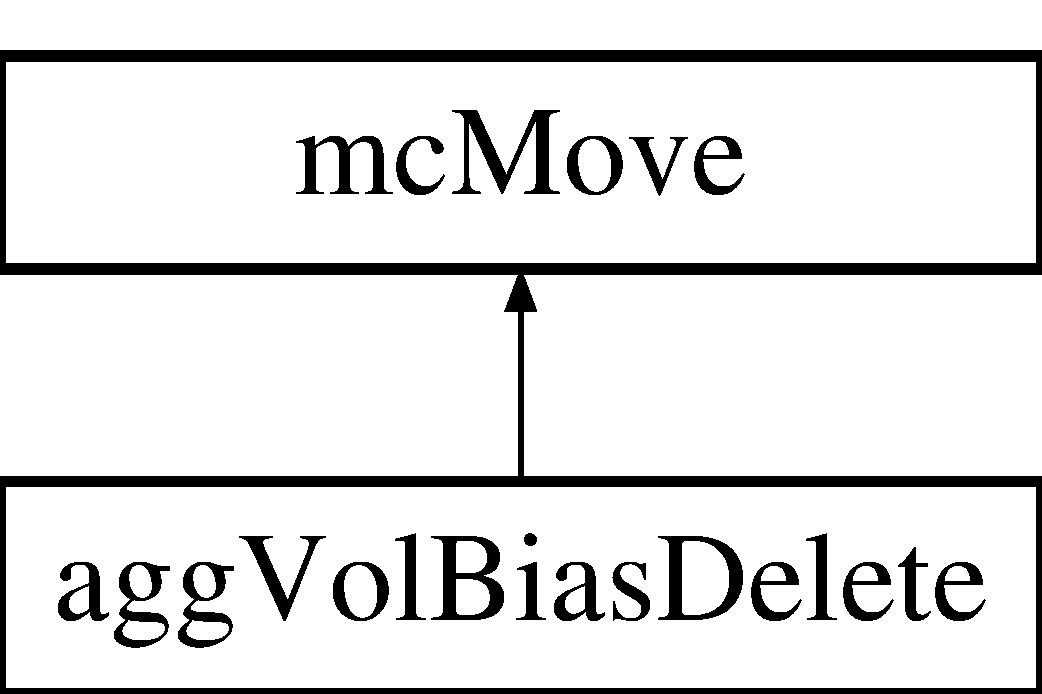
\includegraphics[height=2.000000cm]{classagg_vol_bias_delete}
\end{center}
\end{figure}
\subsection*{Public Member Functions}
\begin{DoxyCompactItemize}
\item 
\hyperlink{classagg_vol_bias_delete_a20979a1dc3c372e9f11daf12330c16cc}{agg\-Vol\-Bias\-Delete} ()
\item 
\hyperlink{classagg_vol_bias_delete_a36412c0e1a86aba8098e0953a64dae3f}{agg\-Vol\-Bias\-Delete} (const int type\-Index, const double p\-Bias, const std\-::vector$<$ double $>$ rc, const std\-::string tag)
\begin{DoxyCompactList}\small\item\em Instantiate a grand canonical aggregation-\/volume bias move to delete particles. \end{DoxyCompactList}\item 
int \hyperlink{classagg_vol_bias_delete_a0692d8bf39ccab1e5e4f0b42c3213e36}{make} (\hyperlink{classsim_system}{sim\-System} \&sys)
\begin{DoxyCompactList}\small\item\em Use aggregation-\/volume bias to delete a particle from the system. \end{DoxyCompactList}\end{DoxyCompactItemize}
\subsection*{Additional Inherited Members}


\subsection{Detailed Description}


Definition at line 39 of file aggvolbias.\-h.



\subsection{Constructor \& Destructor Documentation}
\hypertarget{classagg_vol_bias_delete_a20979a1dc3c372e9f11daf12330c16cc}{\index{agg\-Vol\-Bias\-Delete@{agg\-Vol\-Bias\-Delete}!agg\-Vol\-Bias\-Delete@{agg\-Vol\-Bias\-Delete}}
\index{agg\-Vol\-Bias\-Delete@{agg\-Vol\-Bias\-Delete}!aggVolBiasDelete@{agg\-Vol\-Bias\-Delete}}
\subsubsection[{agg\-Vol\-Bias\-Delete}]{\setlength{\rightskip}{0pt plus 5cm}agg\-Vol\-Bias\-Delete\-::agg\-Vol\-Bias\-Delete (
\begin{DoxyParamCaption}
{}
\end{DoxyParamCaption}
)\hspace{0.3cm}{\ttfamily [inline]}}}\label{classagg_vol_bias_delete_a20979a1dc3c372e9f11daf12330c16cc}


Definition at line 41 of file aggvolbias.\-h.



References mc\-Move\-::change\-N\-\_\-.


\begin{DoxyCode}
41 \{ \hyperlink{classmc_move_add8d6d08be181274a61c7463159ad929}{changeN\_} = \textcolor{keyword}{true}; pBias\_ = 0; \}
\end{DoxyCode}
\hypertarget{classagg_vol_bias_delete_a36412c0e1a86aba8098e0953a64dae3f}{\index{agg\-Vol\-Bias\-Delete@{agg\-Vol\-Bias\-Delete}!agg\-Vol\-Bias\-Delete@{agg\-Vol\-Bias\-Delete}}
\index{agg\-Vol\-Bias\-Delete@{agg\-Vol\-Bias\-Delete}!aggVolBiasDelete@{agg\-Vol\-Bias\-Delete}}
\subsubsection[{agg\-Vol\-Bias\-Delete}]{\setlength{\rightskip}{0pt plus 5cm}agg\-Vol\-Bias\-Delete\-::agg\-Vol\-Bias\-Delete (
\begin{DoxyParamCaption}
\item[{const int}]{type\-Index, }
\item[{const double}]{p\-Bias, }
\item[{const std\-::vector$<$ double $>$}]{rc, }
\item[{const std\-::string}]{tag}
\end{DoxyParamCaption}
)}}\label{classagg_vol_bias_delete_a36412c0e1a86aba8098e0953a64dae3f}


Instantiate a grand canonical aggregation-\/volume bias move to delete particles. 

From Chen et al., J. Chem. Phys. 115 (2001).


\begin{DoxyParams}[1]{Parameters}
\mbox{\tt in}  & {\em type\-Index} & Type to consider deleting from the vicinity of \\
\hline
\mbox{\tt in}  & {\em p\-Bias} & Biasing probability \\
\hline
\mbox{\tt in}  & {\em rc} & Radius (min, max) around particle of type\-Index to consider as being the \char`\"{}in\char`\"{} region \\
\hline
\mbox{\tt in}  & {\em tag} & Name modifier to identify move to user \\
\hline
\end{DoxyParams}


Definition at line 54 of file aggvolbias.\-cpp.



References mc\-Move\-::change\-N\-\_\-, mc\-Move\-::name\-\_\-, and mc\-Move\-::type\-Index\-\_\-.


\begin{DoxyCode}
54                                                                                                            
                          \{
55     \hyperlink{classmc_move_acb731965547b0326ef318ec96da8b46a}{typeIndex\_} = typeIndex;
56         \textcolor{keywordflow}{if} (pBias < 1 && pBias > 0) \{
57                 pBias\_ = pBias;
58         \} \textcolor{keywordflow}{else} \{
59                 \textcolor{keywordflow}{throw} \hyperlink{classcustom_exception}{customException} (\textcolor{stringliteral}{"Bias probability must be > 0 and < 1 for aggVolBias
       moves"});
60         \}
61 
62         \textcolor{keywordflow}{if} (!(rc[0] > 0.0)) \{
63                 \textcolor{keywordflow}{throw} \hyperlink{classcustom_exception}{customException} (\textcolor{stringliteral}{"Min neighborhood radius for aggVolBias must be > 0"})
      ;
64         \} \textcolor{keywordflow}{else} \{
65                 rcmin\_ = rc[0];
66         \}
67 
68         \textcolor{keywordflow}{if} (!(rc[1] > rc[0])) \{
69                 \textcolor{keywordflow}{throw} \hyperlink{classcustom_exception}{customException} (\textcolor{stringliteral}{"Max neighborhood radius for aggVolBias must be > min
      "});
70         \} \textcolor{keywordflow}{else} \{
71                 rcmax\_ = rc[1];
72         \}
73 
74         \hyperlink{classmc_move_ac18c307855e1cb5751bd6e079857a8c5}{name\_} = tag + std::to\_string(typeIndex);
75         \hyperlink{classmc_move_add8d6d08be181274a61c7463159ad929}{changeN\_} = \textcolor{keyword}{true};
76 \}
\end{DoxyCode}


\subsection{Member Function Documentation}
\hypertarget{classagg_vol_bias_delete_a0692d8bf39ccab1e5e4f0b42c3213e36}{\index{agg\-Vol\-Bias\-Delete@{agg\-Vol\-Bias\-Delete}!make@{make}}
\index{make@{make}!aggVolBiasDelete@{agg\-Vol\-Bias\-Delete}}
\subsubsection[{make}]{\setlength{\rightskip}{0pt plus 5cm}int agg\-Vol\-Bias\-Delete\-::make (
\begin{DoxyParamCaption}
\item[{{\bf sim\-System} \&}]{sys}
\end{DoxyParamCaption}
)\hspace{0.3cm}{\ttfamily [virtual]}}}\label{classagg_vol_bias_delete_a0692d8bf39ccab1e5e4f0b42c3213e36}


Use aggregation-\/volume bias to delete a particle from the system. 

All other information is stored in the \hyperlink{classsim_system}{sim\-System} object.


\begin{DoxyParams}[1]{Parameters}
\mbox{\tt in}  & {\em sys} & System object to attempt to delete particles from.\\
\hline
\end{DoxyParams}
\begin{DoxyReturn}{Returns}
M\-O\-V\-E\-\_\-\-S\-U\-C\-C\-E\-S\-S if particle is deleted, otherwise M\-O\-V\-E\-\_\-\-F\-A\-I\-L\-U\-R\-E if not. Will throw exceptions if there was an error. 
\end{DoxyReturn}


Implements \hyperlink{classmc_move_a2e377a628f9ecee5422fc8967d4924eb}{mc\-Move}.



Definition at line 85 of file aggvolbias.\-cpp.



References M\-O\-V\-E\-\_\-\-F\-A\-I\-L\-U\-R\-E.


\begin{DoxyCode}
85                                           \{
86         \textcolor{keywordflow}{return} \hyperlink{moves_8h_a9832cf5fcfa8c0894545b591c9908e39}{MOVE\_FAILURE};
87 \}
\end{DoxyCode}


The documentation for this class was generated from the following files\-:\begin{DoxyCompactItemize}
\item 
/home/nam4/\-Desktop/sandbox/\-F\-H\-M\-C\-Simulation/src/\hyperlink{aggvolbias_8h}{aggvolbias.\-h}\item 
/home/nam4/\-Desktop/sandbox/\-F\-H\-M\-C\-Simulation/src/\hyperlink{aggvolbias_8cpp}{aggvolbias.\-cpp}\end{DoxyCompactItemize}

\hypertarget{classagg_vol_bias_insert}{\section{agg\-Vol\-Bias\-Insert Class Reference}
\label{classagg_vol_bias_insert}\index{agg\-Vol\-Bias\-Insert@{agg\-Vol\-Bias\-Insert}}
}


{\ttfamily \#include $<$aggvolbias.\-h$>$}

Inheritance diagram for agg\-Vol\-Bias\-Insert\-:\begin{figure}[H]
\begin{center}
\leavevmode
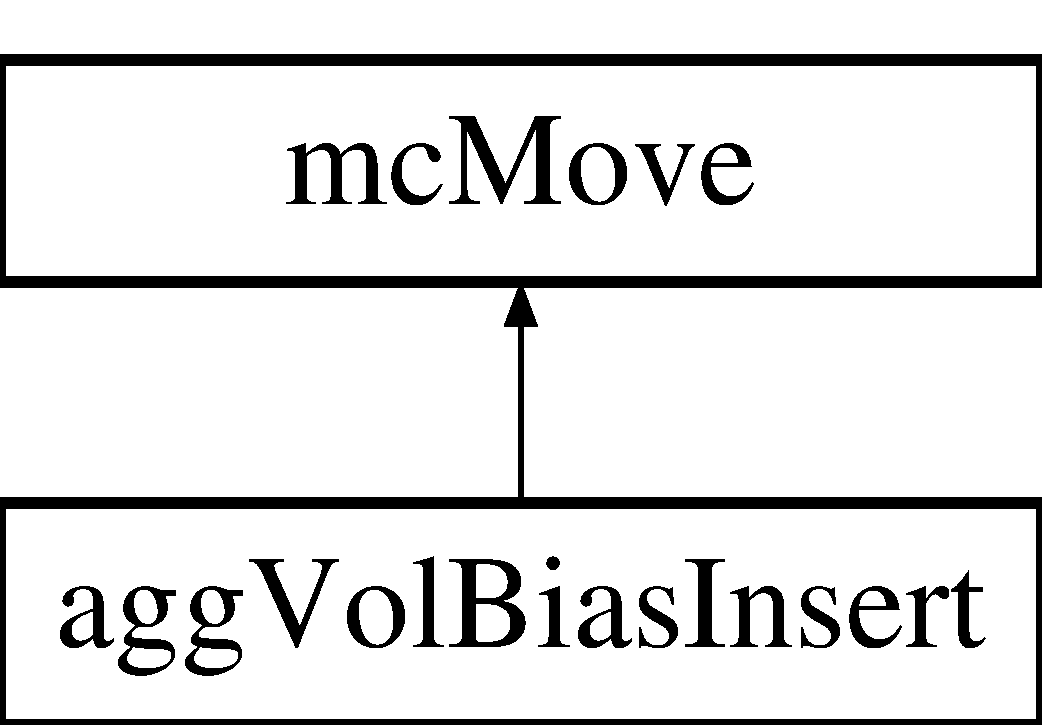
\includegraphics[height=2.000000cm]{classagg_vol_bias_insert}
\end{center}
\end{figure}
\subsection*{Public Member Functions}
\begin{DoxyCompactItemize}
\item 
\hyperlink{classagg_vol_bias_insert_a81ff1f16faebd380b1cb91720781d60a}{agg\-Vol\-Bias\-Insert} ()
\item 
\hyperlink{classagg_vol_bias_insert_ae2aaa1b3422910a395ca101a8d8aef0d}{agg\-Vol\-Bias\-Insert} (const int type\-Index, const double p\-Bias, const std\-::vector$<$ double $>$ rc, const std\-::string tag)
\begin{DoxyCompactList}\small\item\em Instantiate a grand canonical aggregation-\/volume bias move to insert particles. \end{DoxyCompactList}\item 
int \hyperlink{classagg_vol_bias_insert_a09bcb804829321579d40f84b1bfc8856}{make} (\hyperlink{classsim_system}{sim\-System} \&sys)
\begin{DoxyCompactList}\small\item\em Use aggregation-\/volume bias to insert a particle into the system. \end{DoxyCompactList}\end{DoxyCompactItemize}
\subsection*{Additional Inherited Members}


\subsection{Detailed Description}


Definition at line 27 of file aggvolbias.\-h.



\subsection{Constructor \& Destructor Documentation}
\hypertarget{classagg_vol_bias_insert_a81ff1f16faebd380b1cb91720781d60a}{\index{agg\-Vol\-Bias\-Insert@{agg\-Vol\-Bias\-Insert}!agg\-Vol\-Bias\-Insert@{agg\-Vol\-Bias\-Insert}}
\index{agg\-Vol\-Bias\-Insert@{agg\-Vol\-Bias\-Insert}!aggVolBiasInsert@{agg\-Vol\-Bias\-Insert}}
\subsubsection[{agg\-Vol\-Bias\-Insert}]{\setlength{\rightskip}{0pt plus 5cm}agg\-Vol\-Bias\-Insert\-::agg\-Vol\-Bias\-Insert (
\begin{DoxyParamCaption}
{}
\end{DoxyParamCaption}
)\hspace{0.3cm}{\ttfamily [inline]}}}\label{classagg_vol_bias_insert_a81ff1f16faebd380b1cb91720781d60a}


Definition at line 29 of file aggvolbias.\-h.



References mc\-Move\-::change\-N\-\_\-.


\begin{DoxyCode}
29 \{ \hyperlink{classmc_move_add8d6d08be181274a61c7463159ad929}{changeN\_} = \textcolor{keyword}{true}; pBias\_ = 0; \}
\end{DoxyCode}
\hypertarget{classagg_vol_bias_insert_ae2aaa1b3422910a395ca101a8d8aef0d}{\index{agg\-Vol\-Bias\-Insert@{agg\-Vol\-Bias\-Insert}!agg\-Vol\-Bias\-Insert@{agg\-Vol\-Bias\-Insert}}
\index{agg\-Vol\-Bias\-Insert@{agg\-Vol\-Bias\-Insert}!aggVolBiasInsert@{agg\-Vol\-Bias\-Insert}}
\subsubsection[{agg\-Vol\-Bias\-Insert}]{\setlength{\rightskip}{0pt plus 5cm}agg\-Vol\-Bias\-Insert\-::agg\-Vol\-Bias\-Insert (
\begin{DoxyParamCaption}
\item[{const int}]{type\-Index, }
\item[{const double}]{p\-Bias, }
\item[{const std\-::vector$<$ double $>$}]{rc, }
\item[{const std\-::string}]{tag}
\end{DoxyParamCaption}
)}}\label{classagg_vol_bias_insert_ae2aaa1b3422910a395ca101a8d8aef0d}


Instantiate a grand canonical aggregation-\/volume bias move to insert particles. 

From Chen et al., J. Chem. Phys. 115 (2001).


\begin{DoxyParams}[1]{Parameters}
\mbox{\tt in}  & {\em type\-Index} & Type to consider deleting from the vicinity of \\
\hline
\mbox{\tt in}  & {\em p\-Bias} & Biasing probability \\
\hline
\mbox{\tt in}  & {\em rc} & Radius (min, max) around particle of type\-Index to consider as being the \char`\"{}in\char`\"{} region \\
\hline
\mbox{\tt in}  & {\em tag} & Name modifier to identify move to user \\
\hline
\end{DoxyParams}


Definition at line 11 of file aggvolbias.\-cpp.



References mc\-Move\-::change\-N\-\_\-, mc\-Move\-::name\-\_\-, and mc\-Move\-::type\-Index\-\_\-.


\begin{DoxyCode}
11                                                                                                            
                          \{
12     \hyperlink{classmc_move_acb731965547b0326ef318ec96da8b46a}{typeIndex\_} = typeIndex;
13         \textcolor{keywordflow}{if} (pBias < 1 && pBias > 0) \{
14                 pBias\_ = pBias;
15         \} \textcolor{keywordflow}{else} \{
16                 \textcolor{keywordflow}{throw} \hyperlink{classcustom_exception}{customException} (\textcolor{stringliteral}{"Bias probability must be > 0 and < 1 for aggVolBias
       moves"});
17         \}
18 
19         \textcolor{keywordflow}{if} (!(rc[0] > 0.0)) \{
20                 \textcolor{keywordflow}{throw} \hyperlink{classcustom_exception}{customException} (\textcolor{stringliteral}{"Min neighborhood radius for aggVolBias must be > 0"})
      ;
21         \} \textcolor{keywordflow}{else} \{
22                 rcmin\_ = rc[0];
23         \}
24 
25         \textcolor{keywordflow}{if} (!(rc[1] > rc[0])) \{
26                 \textcolor{keywordflow}{throw} \hyperlink{classcustom_exception}{customException} (\textcolor{stringliteral}{"Max neighborhood radius for aggVolBias must be > min
      "});
27         \} \textcolor{keywordflow}{else} \{
28                 rcmax\_ = rc[1];
29         \}
30 
31         \hyperlink{classmc_move_ac18c307855e1cb5751bd6e079857a8c5}{name\_} = tag + std::to\_string(typeIndex);
32         \hyperlink{classmc_move_add8d6d08be181274a61c7463159ad929}{changeN\_} = \textcolor{keyword}{true};
33 \}
\end{DoxyCode}


\subsection{Member Function Documentation}
\hypertarget{classagg_vol_bias_insert_a09bcb804829321579d40f84b1bfc8856}{\index{agg\-Vol\-Bias\-Insert@{agg\-Vol\-Bias\-Insert}!make@{make}}
\index{make@{make}!aggVolBiasInsert@{agg\-Vol\-Bias\-Insert}}
\subsubsection[{make}]{\setlength{\rightskip}{0pt plus 5cm}int agg\-Vol\-Bias\-Insert\-::make (
\begin{DoxyParamCaption}
\item[{{\bf sim\-System} \&}]{sys}
\end{DoxyParamCaption}
)\hspace{0.3cm}{\ttfamily [virtual]}}}\label{classagg_vol_bias_insert_a09bcb804829321579d40f84b1bfc8856}


Use aggregation-\/volume bias to insert a particle into the system. 

All other information is stored in the \hyperlink{classsim_system}{sim\-System} object.


\begin{DoxyParams}[1]{Parameters}
\mbox{\tt in}  & {\em sys} & System object to attempt to insert particles into.\\
\hline
\end{DoxyParams}
\begin{DoxyReturn}{Returns}
M\-O\-V\-E\-\_\-\-S\-U\-C\-C\-E\-S\-S if particle is inserted, otherwise M\-O\-V\-E\-\_\-\-F\-A\-I\-L\-U\-R\-E if not. Will throw exceptions if there was an error. 
\end{DoxyReturn}


Implements \hyperlink{classmc_move_a2e377a628f9ecee5422fc8967d4924eb}{mc\-Move}.



Definition at line 42 of file aggvolbias.\-cpp.



References M\-O\-V\-E\-\_\-\-F\-A\-I\-L\-U\-R\-E.


\begin{DoxyCode}
42                                           \{
43     \textcolor{keywordflow}{return} \hyperlink{moves_8h_a9832cf5fcfa8c0894545b591c9908e39}{MOVE\_FAILURE};
44 \}
\end{DoxyCode}


The documentation for this class was generated from the following files\-:\begin{DoxyCompactItemize}
\item 
/home/nam4/\-Desktop/sandbox/\-F\-H\-M\-C\-Simulation/src/\hyperlink{aggvolbias_8h}{aggvolbias.\-h}\item 
/home/nam4/\-Desktop/sandbox/\-F\-H\-M\-C\-Simulation/src/\hyperlink{aggvolbias_8cpp}{aggvolbias.\-cpp}\end{DoxyCompactItemize}

\hypertarget{classatom}{\section{atom Class Reference}
\label{classatom}\index{atom@{atom}}
}


Atom class with rigid internal degrees of freedom besides its center of mass.  




{\ttfamily \#include $<$atom.\-h$>$}

\subsection*{Public Member Functions}
\begin{DoxyCompactItemize}
\item 
\hyperlink{classatom_a2b63fdf85f714880c6af65b849bdb325}{atom} ()
\item 
\hyperlink{classatom_a5e8b18bca502d3a2a6d79ec5eb8b09ae}{atom} (unsigned int ncenters, std\-::vector$<$ std\-::vector$<$ double $>$ $>$ rel\-\_\-or)
\begin{DoxyCompactList}\small\item\em Instantiate an atom with centers oriented relative to the center. \end{DoxyCompactList}\item 
\hyperlink{classatom_a92f7ce8ce0c3e896e9455a7ceb5e7f85}{$\sim$atom} ()
\item 
void \hyperlink{classatom_a37cbc8cef7998850dc635b4dcbee724c}{rotate\-Centers} (const \hyperlink{classquaternion}{quaternion} \&q)
\end{DoxyCompactItemize}
\subsection*{Data Fields}
\begin{DoxyCompactItemize}
\item 
int \hyperlink{classatom_a3cb00c0c5b7533657e05af6ff4a42740}{m\-State}
\begin{DoxyCompactList}\small\item\em State of fraction insertion of the atom in the expanded ensemble, 0 = fully inserted. \end{DoxyCompactList}\item 
std\-::vector$<$ double $>$ \hyperlink{classatom_a3ae5f4880e7831d8b2c9fda72b4eb24a}{pos}
\begin{DoxyCompactList}\small\item\em 3\-D position \end{DoxyCompactList}\item 
std\-::vector$<$ std\-::vector\\*
$<$ double $>$ $>$ \hyperlink{classatom_a1376d52933b59a61ef76bf47f3f3732f}{vec\-To\-Centers}
\begin{DoxyCompactList}\small\item\em Vectors pointing from pos to rigid centers. \end{DoxyCompactList}\end{DoxyCompactItemize}


\subsection{Detailed Description}
Atom class with rigid internal degrees of freedom besides its center of mass. 

Definition at line 12 of file atom.\-h.



\subsection{Constructor \& Destructor Documentation}
\hypertarget{classatom_a2b63fdf85f714880c6af65b849bdb325}{\index{atom@{atom}!atom@{atom}}
\index{atom@{atom}!atom@{atom}}
\subsubsection[{atom}]{\setlength{\rightskip}{0pt plus 5cm}atom\-::atom (
\begin{DoxyParamCaption}
{}
\end{DoxyParamCaption}
)\hspace{0.3cm}{\ttfamily [inline]}}}\label{classatom_a2b63fdf85f714880c6af65b849bdb325}


Definition at line 14 of file atom.\-h.



References m\-State, and pos.


\begin{DoxyCode}
14 \{ \hyperlink{classatom_a3ae5f4880e7831d8b2c9fda72b4eb24a}{pos}.resize(3, 0); \hyperlink{classatom_a3cb00c0c5b7533657e05af6ff4a42740}{mState} = 0; \} \textcolor{comment}{// assumes no centers}
\end{DoxyCode}
\hypertarget{classatom_a5e8b18bca502d3a2a6d79ec5eb8b09ae}{\index{atom@{atom}!atom@{atom}}
\index{atom@{atom}!atom@{atom}}
\subsubsection[{atom}]{\setlength{\rightskip}{0pt plus 5cm}atom\-::atom (
\begin{DoxyParamCaption}
\item[{unsigned int}]{ncenters, }
\item[{std\-::vector$<$ std\-::vector$<$ double $>$ $>$}]{rel\-Or}
\end{DoxyParamCaption}
)}}\label{classatom_a5e8b18bca502d3a2a6d79ec5eb8b09ae}


Instantiate an atom with centers oriented relative to the center. 


\begin{DoxyParams}[1]{Parameters}
\mbox{\tt in}  & {\em ncenters} & Number of centers /param \mbox{[}in\mbox{]} rel\-Or Vectors pointing to rigid centers from atom's pos \\
\hline
\end{DoxyParams}


Definition at line 11 of file atom.\-cpp.



References vec\-To\-Centers.


\begin{DoxyCode}
11                                                                            \{
12     \textcolor{keywordflow}{try} \{
13         std::vector < double > dummy (3, 0);
14         \hyperlink{classatom_a1376d52933b59a61ef76bf47f3f3732f}{vecToCenters}.resize(ncenters, dummy);
15     \} \textcolor{keywordflow}{catch} (std::bad\_alloc &ba) \{
16         \textcolor{keywordflow}{throw} \hyperlink{classcustom_exception}{customException} (\textcolor{stringliteral}{"Out of memory for atom centers"});
17     \}
18 
19     \textcolor{keywordflow}{if} (relOr.size() != ncenters) \{
20         \textcolor{keywordflow}{throw} \hyperlink{classcustom_exception}{customException} (\textcolor{stringliteral}{"Must specify exactly one 3D orientation for each center"});
21     \} \textcolor{keywordflow}{else} \{
22         \textcolor{keywordflow}{for} (\textcolor{keywordtype}{unsigned} \textcolor{keywordtype}{int} i = 0; i < ncenters; ++i) \{
23             \textcolor{keywordflow}{if} (relOr[i].size() != 3) \{
24                 \textcolor{keywordflow}{throw} \hyperlink{classcustom_exception}{customException} (\textcolor{stringliteral}{"Error - 3D atom center orientations must be in 3D"});
25             \}
26             \textcolor{keywordflow}{for} (\textcolor{keywordtype}{unsigned} \textcolor{keywordtype}{int} j = 0; j < 3; ++j) \{
27                 \hyperlink{classatom_a1376d52933b59a61ef76bf47f3f3732f}{vecToCenters}[i][j] = relOr[i][j];
28             \}
29         \}
30     \}
31 \}
\end{DoxyCode}
\hypertarget{classatom_a92f7ce8ce0c3e896e9455a7ceb5e7f85}{\index{atom@{atom}!$\sim$atom@{$\sim$atom}}
\index{$\sim$atom@{$\sim$atom}!atom@{atom}}
\subsubsection[{$\sim$atom}]{\setlength{\rightskip}{0pt plus 5cm}atom\-::$\sim$atom (
\begin{DoxyParamCaption}
{}
\end{DoxyParamCaption}
)\hspace{0.3cm}{\ttfamily [inline]}}}\label{classatom_a92f7ce8ce0c3e896e9455a7ceb5e7f85}


Definition at line 16 of file atom.\-h.


\begin{DoxyCode}
16 \{\};
\end{DoxyCode}


\subsection{Member Function Documentation}
\hypertarget{classatom_a37cbc8cef7998850dc635b4dcbee724c}{\index{atom@{atom}!rotate\-Centers@{rotate\-Centers}}
\index{rotate\-Centers@{rotate\-Centers}!atom@{atom}}
\subsubsection[{rotate\-Centers}]{\setlength{\rightskip}{0pt plus 5cm}void atom\-::rotate\-Centers (
\begin{DoxyParamCaption}
\item[{const {\bf quaternion} \&}]{q}
\end{DoxyParamCaption}
)}}\label{classatom_a37cbc8cef7998850dc635b4dcbee724c}


\subsection{Field Documentation}
\hypertarget{classatom_a3cb00c0c5b7533657e05af6ff4a42740}{\index{atom@{atom}!m\-State@{m\-State}}
\index{m\-State@{m\-State}!atom@{atom}}
\subsubsection[{m\-State}]{\setlength{\rightskip}{0pt plus 5cm}int atom\-::m\-State}}\label{classatom_a3cb00c0c5b7533657e05af6ff4a42740}


State of fraction insertion of the atom in the expanded ensemble, 0 = fully inserted. 



Definition at line 21 of file atom.\-h.



Referenced by atom(), sim\-System\-::delete\-Atom(), hard\-Wall\-Z\-::energy(), lennard\-Jones\-::energy(), square\-Well\-Wall\-Z\-::energy(), fs\-Lennard\-Jones\-::energy(), cylinder\-Z\-::energy(), tabulated\-::energy(), right\-Triangle\-X\-Z\-::energy(), square\-Well\-::energy(), hard\-Core\-::energy(), sim\-System\-::insert\-Atom(), hard\-Wall\-Z\-::inside(), square\-Well\-Wall\-Z\-::inside(), cylinder\-Z\-::inside(), delete\-Particle\-::make(), insert\-Particle\-::make(), and sanity\-Checks().

\hypertarget{classatom_a3ae5f4880e7831d8b2c9fda72b4eb24a}{\index{atom@{atom}!pos@{pos}}
\index{pos@{pos}!atom@{atom}}
\subsubsection[{pos}]{\setlength{\rightskip}{0pt plus 5cm}std\-::vector$<$ double $>$ atom\-::pos}}\label{classatom_a3ae5f4880e7831d8b2c9fda72b4eb24a}


3\-D position 



Definition at line 22 of file atom.\-h.



Referenced by atom(), hard\-Wall\-Z\-::energy(), lennard\-Jones\-::energy(), square\-Well\-Wall\-Z\-::energy(), fs\-Lennard\-Jones\-::energy(), cylinder\-Z\-::energy(), tabulated\-::energy(), right\-Triangle\-X\-Z\-::energy(), square\-Well\-::energy(), hard\-Core\-::energy(), sim\-System\-::get\-Neighbor\-Atoms(), cell\-List\-::insert\-Particle(), hard\-Wall\-Z\-::inside(), square\-Well\-Wall\-Z\-::inside(), cylinder\-Z\-::inside(), agg\-Vol\-Bias3\-::make(), swap\-Particles\-::make(), insert\-Particle\-::make(), cell\-List\-::swap\-And\-Delete\-Particle(), and cell\-List\-::translate\-Particle().

\hypertarget{classatom_a1376d52933b59a61ef76bf47f3f3732f}{\index{atom@{atom}!vec\-To\-Centers@{vec\-To\-Centers}}
\index{vec\-To\-Centers@{vec\-To\-Centers}!atom@{atom}}
\subsubsection[{vec\-To\-Centers}]{\setlength{\rightskip}{0pt plus 5cm}std\-::vector$<$ std\-::vector $<$ double $>$ $>$ atom\-::vec\-To\-Centers}}\label{classatom_a1376d52933b59a61ef76bf47f3f3732f}


Vectors pointing from pos to rigid centers. 



Definition at line 23 of file atom.\-h.



Referenced by atom().



The documentation for this class was generated from the following files\-:\begin{DoxyCompactItemize}
\item 
/home/nam4/\-Desktop/sandbox/\-F\-H\-M\-C\-Simulation/src/\hyperlink{atom_8h}{atom.\-h}\item 
/home/nam4/\-Desktop/sandbox/\-F\-H\-M\-C\-Simulation/src/\hyperlink{atom_8cpp}{atom.\-cpp}\end{DoxyCompactItemize}

\hypertarget{classbarrier}{\section{barrier Class Reference}
\label{classbarrier}\index{barrier@{barrier}}
}


Virtual base class for barriers.  




{\ttfamily \#include $<$barrier.\-h$>$}

Inheritance diagram for barrier\-:\begin{figure}[H]
\begin{center}
\leavevmode
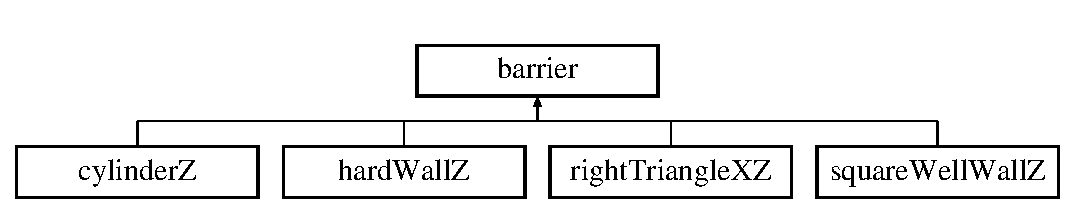
\includegraphics[height=2.000000cm]{classbarrier}
\end{center}
\end{figure}
\subsection*{Public Member Functions}
\begin{DoxyCompactItemize}
\item 
virtual \hyperlink{classbarrier_a54d34bd0e56a4af26ab34975e9569ac7}{$\sim$barrier} ()
\item 
virtual bool \hyperlink{classbarrier_a948ebdcfac501cb75d1a1f045a7d9125}{inside} (const \hyperlink{classatom}{atom} $\ast$a1, const std\-::vector$<$ double $>$ \&box)=0
\item 
virtual double \hyperlink{classbarrier_a2d308cfd5709aa479d0b37733f1a0db7}{energy} (const \hyperlink{classatom}{atom} $\ast$a1, const std\-::vector$<$ double $>$ \&box)=0
\end{DoxyCompactItemize}
\subsection*{Protected Attributes}
\begin{DoxyCompactItemize}
\item 
int \hyperlink{classbarrier_a274cf283ffc97c22ffa9a4258369c400}{M\-\_\-}
\end{DoxyCompactItemize}


\subsection{Detailed Description}
Virtual base class for barriers. 

It is intended that there should be a separate barrier class defined for each species type. 

Definition at line 17 of file barrier.\-h.



\subsection{Constructor \& Destructor Documentation}
\hypertarget{classbarrier_a54d34bd0e56a4af26ab34975e9569ac7}{\index{barrier@{barrier}!$\sim$barrier@{$\sim$barrier}}
\index{$\sim$barrier@{$\sim$barrier}!barrier@{barrier}}
\subsubsection[{$\sim$barrier}]{\setlength{\rightskip}{0pt plus 5cm}virtual barrier\-::$\sim$barrier (
\begin{DoxyParamCaption}
{}
\end{DoxyParamCaption}
)\hspace{0.3cm}{\ttfamily [inline]}, {\ttfamily [virtual]}}}\label{classbarrier_a54d34bd0e56a4af26ab34975e9569ac7}


Definition at line 19 of file barrier.\-h.


\begin{DoxyCode}
19 \{;\}
\end{DoxyCode}


\subsection{Member Function Documentation}
\hypertarget{classbarrier_a2d308cfd5709aa479d0b37733f1a0db7}{\index{barrier@{barrier}!energy@{energy}}
\index{energy@{energy}!barrier@{barrier}}
\subsubsection[{energy}]{\setlength{\rightskip}{0pt plus 5cm}virtual double barrier\-::energy (
\begin{DoxyParamCaption}
\item[{const {\bf atom} $\ast$}]{a1, }
\item[{const std\-::vector$<$ double $>$ \&}]{box}
\end{DoxyParamCaption}
)\hspace{0.3cm}{\ttfamily [pure virtual]}}}\label{classbarrier_a2d308cfd5709aa479d0b37733f1a0db7}


Implemented in \hyperlink{classright_triangle_x_z_a0a15ebff4238aeb15cad052cf9904f43}{right\-Triangle\-X\-Z}, \hyperlink{classcylinder_z_a0d1ec094ac9bf23b74e6f03f09477217}{cylinder\-Z}, \hyperlink{classsquare_well_wall_z_a77c366eb9c10f6a68e3f633e9b64dc47}{square\-Well\-Wall\-Z}, and \hyperlink{classhard_wall_z_ae1c05d46be694e7b071969f9511e4142}{hard\-Wall\-Z}.

\hypertarget{classbarrier_a948ebdcfac501cb75d1a1f045a7d9125}{\index{barrier@{barrier}!inside@{inside}}
\index{inside@{inside}!barrier@{barrier}}
\subsubsection[{inside}]{\setlength{\rightskip}{0pt plus 5cm}virtual bool barrier\-::inside (
\begin{DoxyParamCaption}
\item[{const {\bf atom} $\ast$}]{a1, }
\item[{const std\-::vector$<$ double $>$ \&}]{box}
\end{DoxyParamCaption}
)\hspace{0.3cm}{\ttfamily [pure virtual]}}}\label{classbarrier_a948ebdcfac501cb75d1a1f045a7d9125}


Implemented in \hyperlink{classright_triangle_x_z_a574bcc38639a6d599aaa38fd9085ff63}{right\-Triangle\-X\-Z}, \hyperlink{classcylinder_z_aff84684096c1d04d73ee894b499a0a2f}{cylinder\-Z}, \hyperlink{classsquare_well_wall_z_a10fc7a357ac1ec6bb0cd1d1e95570195}{square\-Well\-Wall\-Z}, and \hyperlink{classhard_wall_z_ac4c72aa32e0cdfe40c6765642ffb78d7}{hard\-Wall\-Z}.



\subsection{Field Documentation}
\hypertarget{classbarrier_a274cf283ffc97c22ffa9a4258369c400}{\index{barrier@{barrier}!M\-\_\-@{M\-\_\-}}
\index{M\-\_\-@{M\-\_\-}!barrier@{barrier}}
\subsubsection[{M\-\_\-}]{\setlength{\rightskip}{0pt plus 5cm}int barrier\-::\-M\-\_\-\hspace{0.3cm}{\ttfamily [protected]}}}\label{classbarrier_a274cf283ffc97c22ffa9a4258369c400}


Definition at line 24 of file barrier.\-h.



Referenced by cylinder\-Z\-::cylinder\-Z(), hard\-Wall\-Z\-::energy(), square\-Well\-Wall\-Z\-::energy(), cylinder\-Z\-::energy(), right\-Triangle\-X\-Z\-::energy(), hard\-Wall\-Z\-::hard\-Wall\-Z(), hard\-Wall\-Z\-::inside(), square\-Well\-Wall\-Z\-::inside(), cylinder\-Z\-::inside(), right\-Triangle\-X\-Z\-::right\-Triangle\-X\-Z(), and square\-Well\-Wall\-Z\-::square\-Well\-Wall\-Z().



The documentation for this class was generated from the following file\-:\begin{DoxyCompactItemize}
\item 
/home/nam4/\-Desktop/sandbox/\-F\-H\-M\-C\-Simulation/src/\hyperlink{barrier_8h}{barrier.\-h}\end{DoxyCompactItemize}

\hypertarget{classcell_list}{\section{cell\-List Class Reference}
\label{classcell_list}\index{cell\-List@{cell\-List}}
}


\hyperlink{classcell_list}{cell\-List} class.  




{\ttfamily \#include $<$cell\-List.\-h$>$}

\subsection*{Public Member Functions}
\begin{DoxyCompactItemize}
\item 
\hyperlink{classcell_list_abae34854b8fcdeaaf2dc8de2ee47de94}{cell\-List} (std\-::vector$<$ double $>$, double, std\-::vector$<$ \hyperlink{classatom}{atom} $\ast$ $>$)
\item 
void \hyperlink{classcell_list_a58c091eb874dd1b88558bb92424e5ef2}{sort\-Into\-Cells} (std\-::vector$<$ \hyperlink{classatom}{atom} $\ast$ $>$)
\item 
void \hyperlink{classcell_list_ac4400cd9b80c3199e6482e8bcb1990c6}{sort\-Into\-Cells} (std\-::vector$<$ \hyperlink{classatom}{atom} $>$ $\ast$)
\item 
void \hyperlink{classcell_list_a56c0012eed483e47248f9065bfc70fce}{insert\-Particle} (\hyperlink{classatom}{atom} $\ast$)
\item 
void \hyperlink{classcell_list_a31caca1e8dd05c33215ac7495d55aeea}{swap\-And\-Delete\-Particle} (\hyperlink{classatom}{atom} $\ast$, \hyperlink{classatom}{atom} $\ast$)
\item 
void \hyperlink{classcell_list_a0d77368abdd5a4665ca2302b9a20509b}{translate\-Particle} (\hyperlink{classatom}{atom} $\ast$, std\-::vector$<$ double $>$)
\item 
int \hyperlink{classcell_list_aa6b843131cd487164a137571c7343cab}{calc\-Index} (int, int, int)
\item 
int \hyperlink{classcell_list_a9a5f8f84d17a8f0f7d3791aa64b75803}{calc\-Index\-S} (int, int, int)
\item 
int \hyperlink{classcell_list_a01dbd9a86ec24293d369be8d67b9df70}{calc\-Index} (double, double, double)
\item 
int \hyperlink{classcell_list_a7df926ebf382f281d15935550ffcba64}{calc\-Index\-S} (double, double, double)
\end{DoxyCompactItemize}
\subsection*{Data Fields}
\begin{DoxyCompactItemize}
\item 
std\-::vector$<$ double $>$ \hyperlink{classcell_list_ac920f36bcf43f79ab853921bb0b7c2f4}{cell\-Size}
\item 
std\-::vector$<$ double $>$ \hyperlink{classcell_list_ae65748b80d5e06edfa22daaf569f2757}{box}
\item 
int \hyperlink{classcell_list_a342f802c342f51f3c1aa4dab7d7a4d84}{cell\-Count\-X}
\item 
int \hyperlink{classcell_list_aa0c942e7b0b61cda1d688ffc96e8f1c8}{cell\-Count\-Y}
\item 
int \hyperlink{classcell_list_a2b506715c6ded7cb9fadf994f4f01785}{cell\-Count\-Z}
\item 
int \hyperlink{classcell_list_a619d607f8569876cead1bdfad239d4b2}{cell\-Count\-X\-Y}
\item 
int \hyperlink{classcell_list_a6a695015c180229cd491db58c6e18ff4}{cell\-Count}
\item 
std\-::vector$<$ std\-::vector$<$ \hyperlink{classatom}{atom} $\ast$ $>$ $>$ \hyperlink{classcell_list_a10bc0c3ae819293b1e88bc7d1bfdb2aa}{cells}
\item 
std\-::vector$<$ std\-::vector\\*
$<$ unsigned int $>$ $>$ \hyperlink{classcell_list_ada607886d0e5a20d710dde694d6d989f}{neighbours}
\end{DoxyCompactItemize}


\subsection{Detailed Description}
\hyperlink{classcell_list}{cell\-List} class. 

Definition at line 15 of file cell\-List.\-h.



\subsection{Constructor \& Destructor Documentation}
\hypertarget{classcell_list_abae34854b8fcdeaaf2dc8de2ee47de94}{\index{cell\-List@{cell\-List}!cell\-List@{cell\-List}}
\index{cell\-List@{cell\-List}!cellList@{cell\-List}}
\subsubsection[{cell\-List}]{\setlength{\rightskip}{0pt plus 5cm}cell\-List\-::cell\-List (
\begin{DoxyParamCaption}
\item[{std\-::vector$<$ double $>$}]{\-\_\-box, }
\item[{double}]{\-\_\-cell\-Size, }
\item[{std\-::vector$<$ {\bf atom} $\ast$ $>$}]{\-\_\-atoms}
\end{DoxyParamCaption}
)}}\label{classcell_list_abae34854b8fcdeaaf2dc8de2ee47de94}


Definition at line 3 of file cell\-List.\-cpp.



References box, cell\-Count, cell\-Count\-X, cell\-Count\-X\-Y, cell\-Count\-Y, cell\-Count\-Z, cells, cell\-Size, neighbours, and sort\-Into\-Cells().


\begin{DoxyCode}
3                                                                                           \{
4     \hyperlink{classcell_list_ae65748b80d5e06edfa22daaf569f2757}{box} = \_box;
5     \hyperlink{classcell_list_a342f802c342f51f3c1aa4dab7d7a4d84}{cellCountX} = floor(\_box[0]/\_cellSize);
6     \hyperlink{classcell_list_aa0c942e7b0b61cda1d688ffc96e8f1c8}{cellCountY} = floor(\_box[1]/\_cellSize);
7     \hyperlink{classcell_list_a2b506715c6ded7cb9fadf994f4f01785}{cellCountZ} = floor(\_box[2]/\_cellSize);
8     \hyperlink{classcell_list_a619d607f8569876cead1bdfad239d4b2}{cellCountXY} = \hyperlink{classcell_list_a342f802c342f51f3c1aa4dab7d7a4d84}{cellCountX}*\hyperlink{classcell_list_aa0c942e7b0b61cda1d688ffc96e8f1c8}{cellCountY};
9     \hyperlink{classcell_list_a6a695015c180229cd491db58c6e18ff4}{cellCount} = \hyperlink{classcell_list_a619d607f8569876cead1bdfad239d4b2}{cellCountXY}*\hyperlink{classcell_list_a2b506715c6ded7cb9fadf994f4f01785}{cellCountZ};
10 
11     \hyperlink{classcell_list_ac920f36bcf43f79ab853921bb0b7c2f4}{cellSize}.resize(3);
12     \hyperlink{classcell_list_ac920f36bcf43f79ab853921bb0b7c2f4}{cellSize}[0] = \_box[0]/\hyperlink{classcell_list_a342f802c342f51f3c1aa4dab7d7a4d84}{cellCountX};
13     \hyperlink{classcell_list_ac920f36bcf43f79ab853921bb0b7c2f4}{cellSize}[1] = \_box[1]/\hyperlink{classcell_list_aa0c942e7b0b61cda1d688ffc96e8f1c8}{cellCountY};
14     \hyperlink{classcell_list_ac920f36bcf43f79ab853921bb0b7c2f4}{cellSize}[2] = \_box[2]/\hyperlink{classcell_list_a2b506715c6ded7cb9fadf994f4f01785}{cellCountZ};
15 
16     \textcolor{comment}{// init neighbour list}
17     \hyperlink{classcell_list_ada607886d0e5a20d710dde694d6d989f}{neighbours}.assign(\hyperlink{classcell_list_a6a695015c180229cd491db58c6e18ff4}{cellCount}, std::vector < unsigned int > (26));
18     initNeighbours();
19 
20     \textcolor{comment}{// init cell list}
21     \hyperlink{classcell_list_a10bc0c3ae819293b1e88bc7d1bfdb2aa}{cells}.assign(\hyperlink{classcell_list_a6a695015c180229cd491db58c6e18ff4}{cellCount}, std::vector < atom* > (0));
22 
23     \textcolor{comment}{// clear all cells}
24     \textcolor{keyword}{const} \textcolor{keywordtype}{unsigned} \textcolor{keywordtype}{int} reserveCount = ceil(\hyperlink{classcell_list_ac920f36bcf43f79ab853921bb0b7c2f4}{cellSize}[0]*\hyperlink{classcell_list_ac920f36bcf43f79ab853921bb0b7c2f4}{cellSize}[1]*
      \hyperlink{classcell_list_ac920f36bcf43f79ab853921bb0b7c2f4}{cellSize}[2]);
25     \textcolor{keywordflow}{for} (\textcolor{keywordtype}{unsigned} \textcolor{keywordtype}{int} i = 0; i < \hyperlink{classcell_list_a10bc0c3ae819293b1e88bc7d1bfdb2aa}{cells}.size(); i++) \{
26         \hyperlink{classcell_list_a10bc0c3ae819293b1e88bc7d1bfdb2aa}{cells}[i].reserve(reserveCount);
27         \hyperlink{classcell_list_a10bc0c3ae819293b1e88bc7d1bfdb2aa}{cells}[i].clear();
28     \}
29 
30     \textcolor{keywordflow}{if} (\_atoms.size() > 0) \{
31         \textcolor{comment}{//std::cout << "Sorting particles into cells." << std::endl;}
32         \hyperlink{classcell_list_a58c091eb874dd1b88558bb92424e5ef2}{sortIntoCells}(\_atoms);
33     \}
34 \}
\end{DoxyCode}


\subsection{Member Function Documentation}
\hypertarget{classcell_list_aa6b843131cd487164a137571c7343cab}{\index{cell\-List@{cell\-List}!calc\-Index@{calc\-Index}}
\index{calc\-Index@{calc\-Index}!cellList@{cell\-List}}
\subsubsection[{calc\-Index}]{\setlength{\rightskip}{0pt plus 5cm}int cell\-List\-::calc\-Index (
\begin{DoxyParamCaption}
\item[{int}]{k, }
\item[{int}]{l, }
\item[{int}]{m}
\end{DoxyParamCaption}
)\hspace{0.3cm}{\ttfamily [inline]}}}\label{classcell_list_aa6b843131cd487164a137571c7343cab}


Definition at line 41 of file cell\-List.\-h.



References cell\-Count\-X, and cell\-Count\-X\-Y.



Referenced by sim\-System\-::get\-Neighbor\-Atoms(), insert\-Particle(), sort\-Into\-Cells(), swap\-And\-Delete\-Particle(), and translate\-Particle().


\begin{DoxyCode}
41                                                    \{
42     \textcolor{keywordflow}{return} (k + l*\hyperlink{classcell_list_a342f802c342f51f3c1aa4dab7d7a4d84}{cellCountX} + m*\hyperlink{classcell_list_a619d607f8569876cead1bdfad239d4b2}{cellCountXY});
43 \}
\end{DoxyCode}
\hypertarget{classcell_list_a01dbd9a86ec24293d369be8d67b9df70}{\index{cell\-List@{cell\-List}!calc\-Index@{calc\-Index}}
\index{calc\-Index@{calc\-Index}!cellList@{cell\-List}}
\subsubsection[{calc\-Index}]{\setlength{\rightskip}{0pt plus 5cm}int cell\-List\-::calc\-Index (
\begin{DoxyParamCaption}
\item[{double}]{\-\_\-x, }
\item[{double}]{\-\_\-y, }
\item[{double}]{\-\_\-z}
\end{DoxyParamCaption}
)\hspace{0.3cm}{\ttfamily [inline]}}}\label{classcell_list_a01dbd9a86ec24293d369be8d67b9df70}


Definition at line 69 of file cell\-List.\-h.



References cell\-Count\-X, cell\-Count\-X\-Y, and cell\-Size.


\begin{DoxyCode}
69                                                                \{
70     \textcolor{keywordflow}{return} (floor(\_x/\hyperlink{classcell_list_ac920f36bcf43f79ab853921bb0b7c2f4}{cellSize}[0]) + floor(\_y/\hyperlink{classcell_list_ac920f36bcf43f79ab853921bb0b7c2f4}{cellSize}[1])*
      \hyperlink{classcell_list_a342f802c342f51f3c1aa4dab7d7a4d84}{cellCountX} +floor(\_z/\hyperlink{classcell_list_ac920f36bcf43f79ab853921bb0b7c2f4}{cellSize}[2])*\hyperlink{classcell_list_a619d607f8569876cead1bdfad239d4b2}{cellCountXY});
71 \}
\end{DoxyCode}
\hypertarget{classcell_list_a9a5f8f84d17a8f0f7d3791aa64b75803}{\index{cell\-List@{cell\-List}!calc\-Index\-S@{calc\-Index\-S}}
\index{calc\-Index\-S@{calc\-Index\-S}!cellList@{cell\-List}}
\subsubsection[{calc\-Index\-S}]{\setlength{\rightskip}{0pt plus 5cm}int cell\-List\-::calc\-Index\-S (
\begin{DoxyParamCaption}
\item[{int}]{\-\_\-k, }
\item[{int}]{\-\_\-l, }
\item[{int}]{\-\_\-m}
\end{DoxyParamCaption}
)\hspace{0.3cm}{\ttfamily [inline]}}}\label{classcell_list_a9a5f8f84d17a8f0f7d3791aa64b75803}


Definition at line 46 of file cell\-List.\-h.



References cell\-Count\-X, cell\-Count\-X\-Y, cell\-Count\-Y, and cell\-Count\-Z.


\begin{DoxyCode}
46                                                        \{
47     \textcolor{keywordtype}{int} k = \_k;
48     \textcolor{keywordtype}{int} l = \_l;
49     \textcolor{keywordtype}{int} m = \_m;
50 
51     \textcolor{keywordflow}{if} (k >= \hyperlink{classcell_list_a342f802c342f51f3c1aa4dab7d7a4d84}{cellCountX})
52         k -= \hyperlink{classcell_list_a342f802c342f51f3c1aa4dab7d7a4d84}{cellCountX};
53     \textcolor{keywordflow}{else} \textcolor{keywordflow}{if} (k < 0)
54         k += \hyperlink{classcell_list_a342f802c342f51f3c1aa4dab7d7a4d84}{cellCountX};
55 
56     \textcolor{keywordflow}{if} (l >= \hyperlink{classcell_list_aa0c942e7b0b61cda1d688ffc96e8f1c8}{cellCountY})
57         l -= \hyperlink{classcell_list_aa0c942e7b0b61cda1d688ffc96e8f1c8}{cellCountY};
58     \textcolor{keywordflow}{else} \textcolor{keywordflow}{if} (l < 0)
59         l += \hyperlink{classcell_list_aa0c942e7b0b61cda1d688ffc96e8f1c8}{cellCountY};
60 
61     \textcolor{keywordflow}{if} (m >= \hyperlink{classcell_list_a2b506715c6ded7cb9fadf994f4f01785}{cellCountZ})
62         m -= \hyperlink{classcell_list_a2b506715c6ded7cb9fadf994f4f01785}{cellCountZ};
63     \textcolor{keywordflow}{else} \textcolor{keywordflow}{if} (m < 0)
64         m += \hyperlink{classcell_list_a2b506715c6ded7cb9fadf994f4f01785}{cellCountZ};
65 
66     \textcolor{keywordflow}{return} (k + l*\hyperlink{classcell_list_a342f802c342f51f3c1aa4dab7d7a4d84}{cellCountX} + m*\hyperlink{classcell_list_a619d607f8569876cead1bdfad239d4b2}{cellCountXY});
67 \}
\end{DoxyCode}
\hypertarget{classcell_list_a7df926ebf382f281d15935550ffcba64}{\index{cell\-List@{cell\-List}!calc\-Index\-S@{calc\-Index\-S}}
\index{calc\-Index\-S@{calc\-Index\-S}!cellList@{cell\-List}}
\subsubsection[{calc\-Index\-S}]{\setlength{\rightskip}{0pt plus 5cm}int cell\-List\-::calc\-Index\-S (
\begin{DoxyParamCaption}
\item[{double}]{\-\_\-x, }
\item[{double}]{\-\_\-y, }
\item[{double}]{\-\_\-z}
\end{DoxyParamCaption}
)\hspace{0.3cm}{\ttfamily [inline]}}}\label{classcell_list_a7df926ebf382f281d15935550ffcba64}


Definition at line 74 of file cell\-List.\-h.



References box, cell\-Count\-X, cell\-Count\-X\-Y, and cell\-Size.


\begin{DoxyCode}
74                                                                 \{
75     \textcolor{keywordtype}{double} x = \_x;
76     \textcolor{keywordtype}{double} y = \_y;
77     \textcolor{keywordtype}{double} z = \_z;
78 
79     \textcolor{keywordflow}{if} (x >= \hyperlink{classcell_list_ae65748b80d5e06edfa22daaf569f2757}{box}[0])
80         x -= \hyperlink{classcell_list_ae65748b80d5e06edfa22daaf569f2757}{box}[0];
81     \textcolor{keywordflow}{else} \textcolor{keywordflow}{if} (x < 0.0)
82         x += \hyperlink{classcell_list_ae65748b80d5e06edfa22daaf569f2757}{box}[0];
83 
84     \textcolor{keywordflow}{if} (y >= \hyperlink{classcell_list_ae65748b80d5e06edfa22daaf569f2757}{box}[1])
85         y -= \hyperlink{classcell_list_ae65748b80d5e06edfa22daaf569f2757}{box}[1];
86     \textcolor{keywordflow}{else} \textcolor{keywordflow}{if} (y < 0.0)
87         y += \hyperlink{classcell_list_ae65748b80d5e06edfa22daaf569f2757}{box}[1];
88 
89     \textcolor{keywordflow}{if} (z >= \hyperlink{classcell_list_ae65748b80d5e06edfa22daaf569f2757}{box}[2])
90         z -= \hyperlink{classcell_list_ae65748b80d5e06edfa22daaf569f2757}{box}[2];
91     \textcolor{keywordflow}{else} \textcolor{keywordflow}{if} (z < 0.0)
92         z += \hyperlink{classcell_list_ae65748b80d5e06edfa22daaf569f2757}{box}[2];
93 
94     \textcolor{keywordflow}{return} (floor(x/\hyperlink{classcell_list_ac920f36bcf43f79ab853921bb0b7c2f4}{cellSize}[0]) + floor(y/\hyperlink{classcell_list_ac920f36bcf43f79ab853921bb0b7c2f4}{cellSize}[1])*
      \hyperlink{classcell_list_a342f802c342f51f3c1aa4dab7d7a4d84}{cellCountX} +floor(z/\hyperlink{classcell_list_ac920f36bcf43f79ab853921bb0b7c2f4}{cellSize}[2])*\hyperlink{classcell_list_a619d607f8569876cead1bdfad239d4b2}{cellCountXY});
95 \}
\end{DoxyCode}
\hypertarget{classcell_list_a56c0012eed483e47248f9065bfc70fce}{\index{cell\-List@{cell\-List}!insert\-Particle@{insert\-Particle}}
\index{insert\-Particle@{insert\-Particle}!cellList@{cell\-List}}
\subsubsection[{insert\-Particle}]{\setlength{\rightskip}{0pt plus 5cm}void cell\-List\-::insert\-Particle (
\begin{DoxyParamCaption}
\item[{{\bf atom} $\ast$}]{\-\_\-a}
\end{DoxyParamCaption}
)}}\label{classcell_list_a56c0012eed483e47248f9065bfc70fce}


Definition at line 94 of file cell\-List.\-cpp.



References calc\-Index(), cells, and atom\-::pos.



Referenced by sim\-System\-::insert\-Atom().


\begin{DoxyCode}
94                                        \{
95     \textcolor{keyword}{const} \textcolor{keywordtype}{unsigned} index = \hyperlink{classcell_list_aa6b843131cd487164a137571c7343cab}{calcIndex}(\_a->\hyperlink{classatom_a3ae5f4880e7831d8b2c9fda72b4eb24a}{pos}[0], \_a->\hyperlink{classatom_a3ae5f4880e7831d8b2c9fda72b4eb24a}{pos}[1], \_a->
      \hyperlink{classatom_a3ae5f4880e7831d8b2c9fda72b4eb24a}{pos}[2]);
96     \hyperlink{classcell_list_a10bc0c3ae819293b1e88bc7d1bfdb2aa}{cells}[index].push\_back(\_a);
97 \}
\end{DoxyCode}
\hypertarget{classcell_list_a58c091eb874dd1b88558bb92424e5ef2}{\index{cell\-List@{cell\-List}!sort\-Into\-Cells@{sort\-Into\-Cells}}
\index{sort\-Into\-Cells@{sort\-Into\-Cells}!cellList@{cell\-List}}
\subsubsection[{sort\-Into\-Cells}]{\setlength{\rightskip}{0pt plus 5cm}void cell\-List\-::sort\-Into\-Cells (
\begin{DoxyParamCaption}
\item[{std\-::vector$<$ {\bf atom} $\ast$ $>$}]{\-\_\-atoms}
\end{DoxyParamCaption}
)}}\label{classcell_list_a58c091eb874dd1b88558bb92424e5ef2}


Definition at line 72 of file cell\-List.\-cpp.



References calc\-Index(), and cells.



Referenced by cell\-List().


\begin{DoxyCode}
72                                                         \{
73     \textcolor{comment}{// clear all cells}
74     \textcolor{keywordflow}{for} (\textcolor{keywordtype}{unsigned} \textcolor{keywordtype}{int} i = 0; i < \hyperlink{classcell_list_a10bc0c3ae819293b1e88bc7d1bfdb2aa}{cells}.size(); i++)
75         \hyperlink{classcell_list_a10bc0c3ae819293b1e88bc7d1bfdb2aa}{cells}[i].clear();
76 
77     \textcolor{keywordflow}{for} (\textcolor{keywordtype}{unsigned} \textcolor{keywordtype}{int} i=0; i<\_atoms.size(); i++) \{
78         \textcolor{keyword}{const} \textcolor{keywordtype}{unsigned} index = \hyperlink{classcell_list_aa6b843131cd487164a137571c7343cab}{calcIndex}(\_atoms[i]->pos[0], \_atoms[i]->pos[1], \_atoms[i]->pos[2]);
79         \hyperlink{classcell_list_a10bc0c3ae819293b1e88bc7d1bfdb2aa}{cells}[index].push\_back(\_atoms[i]);
80     \}
81 \}
\end{DoxyCode}
\hypertarget{classcell_list_ac4400cd9b80c3199e6482e8bcb1990c6}{\index{cell\-List@{cell\-List}!sort\-Into\-Cells@{sort\-Into\-Cells}}
\index{sort\-Into\-Cells@{sort\-Into\-Cells}!cellList@{cell\-List}}
\subsubsection[{sort\-Into\-Cells}]{\setlength{\rightskip}{0pt plus 5cm}void cell\-List\-::sort\-Into\-Cells (
\begin{DoxyParamCaption}
\item[{std\-::vector$<$ {\bf atom} $>$ $\ast$}]{\-\_\-atoms}
\end{DoxyParamCaption}
)}}\label{classcell_list_ac4400cd9b80c3199e6482e8bcb1990c6}


Definition at line 83 of file cell\-List.\-cpp.



References calc\-Index(), and cells.


\begin{DoxyCode}
83                                                         \{
84     \textcolor{comment}{// clear all cells}
85     \textcolor{keywordflow}{for} (\textcolor{keywordtype}{unsigned} \textcolor{keywordtype}{int} i = 0; i < \hyperlink{classcell_list_a10bc0c3ae819293b1e88bc7d1bfdb2aa}{cells}.size(); i++)
86         \hyperlink{classcell_list_a10bc0c3ae819293b1e88bc7d1bfdb2aa}{cells}[i].clear();
87 
88     \textcolor{keywordflow}{for} (\textcolor{keywordtype}{unsigned} \textcolor{keywordtype}{int} i = 0; i < \_atoms->size(); i++) \{
89         \textcolor{keyword}{const} \textcolor{keywordtype}{unsigned} index = \hyperlink{classcell_list_aa6b843131cd487164a137571c7343cab}{calcIndex}(\_atoms->at(i).pos[0], \_atoms->at(i).pos[1], \_atoms->at(i)
      .pos[2]);
90         \hyperlink{classcell_list_a10bc0c3ae819293b1e88bc7d1bfdb2aa}{cells}[index].push\_back(&\_atoms->at(i));
91     \}
92 \}
\end{DoxyCode}
\hypertarget{classcell_list_a31caca1e8dd05c33215ac7495d55aeea}{\index{cell\-List@{cell\-List}!swap\-And\-Delete\-Particle@{swap\-And\-Delete\-Particle}}
\index{swap\-And\-Delete\-Particle@{swap\-And\-Delete\-Particle}!cellList@{cell\-List}}
\subsubsection[{swap\-And\-Delete\-Particle}]{\setlength{\rightskip}{0pt plus 5cm}void cell\-List\-::swap\-And\-Delete\-Particle (
\begin{DoxyParamCaption}
\item[{{\bf atom} $\ast$}]{\-\_\-a, }
\item[{{\bf atom} $\ast$}]{\-\_\-b}
\end{DoxyParamCaption}
)}}\label{classcell_list_a31caca1e8dd05c33215ac7495d55aeea}


Definition at line 101 of file cell\-List.\-cpp.



References calc\-Index(), cells, and atom\-::pos.



Referenced by sim\-System\-::delete\-Atom().


\begin{DoxyCode}
101                                                         \{
102     \textcolor{keyword}{const} \textcolor{keywordtype}{unsigned} indexA = \hyperlink{classcell_list_aa6b843131cd487164a137571c7343cab}{calcIndex}(\_a->\hyperlink{classatom_a3ae5f4880e7831d8b2c9fda72b4eb24a}{pos}[0], \_a->\hyperlink{classatom_a3ae5f4880e7831d8b2c9fda72b4eb24a}{pos}[1], \_a->
      \hyperlink{classatom_a3ae5f4880e7831d8b2c9fda72b4eb24a}{pos}[2]);
103     \textcolor{keyword}{const} \textcolor{keywordtype}{unsigned} indexB = \hyperlink{classcell_list_aa6b843131cd487164a137571c7343cab}{calcIndex}(\_b->\hyperlink{classatom_a3ae5f4880e7831d8b2c9fda72b4eb24a}{pos}[0], \_b->\hyperlink{classatom_a3ae5f4880e7831d8b2c9fda72b4eb24a}{pos}[1], \_b->
      \hyperlink{classatom_a3ae5f4880e7831d8b2c9fda72b4eb24a}{pos}[2]);
104 
105     \textcolor{keywordtype}{unsigned} \textcolor{keywordtype}{int} cellIndexA = 0, cellIndexB = 0;
106     \textcolor{keywordtype}{bool} foundCellIndexA = \textcolor{keyword}{false}, foundCellIndexB = \textcolor{keyword}{false};
107 
108     \textcolor{comment}{// locate position of atom \_a in its cell}
109     \textcolor{keywordflow}{for} (\textcolor{keywordtype}{unsigned} \textcolor{keywordtype}{int} i = 0; i < \hyperlink{classcell_list_a10bc0c3ae819293b1e88bc7d1bfdb2aa}{cells}[indexA].size(); i++) \{ \textcolor{comment}{// error?}
110         \textcolor{keywordflow}{if} (\hyperlink{classcell_list_a10bc0c3ae819293b1e88bc7d1bfdb2aa}{cells}[indexA][i] == \_a) \{
111             cellIndexA = i;
112             foundCellIndexA = \textcolor{keyword}{true};
113             \textcolor{keywordflow}{break};
114         \}
115     \}
116 
117     \textcolor{comment}{// locate position of atom \_b in its cell}
118     \textcolor{keywordflow}{for} (\textcolor{keywordtype}{unsigned} \textcolor{keywordtype}{int} i = 0; i < \hyperlink{classcell_list_a10bc0c3ae819293b1e88bc7d1bfdb2aa}{cells}[indexB].size(); i++) \{ \textcolor{comment}{// error ?}
119         \textcolor{keywordflow}{if} (\hyperlink{classcell_list_a10bc0c3ae819293b1e88bc7d1bfdb2aa}{cells}[indexB][i] == \_b) \{
120             cellIndexB = i;
121             foundCellIndexB = \textcolor{keyword}{true};
122             \textcolor{keywordflow}{break};
123         \}
124     \}
125 
126     \textcolor{keywordflow}{if} (!foundCellIndexA || !foundCellIndexB) \{
127         \textcolor{keywordflow}{throw} \hyperlink{classcustom_exception}{customException} (\textcolor{stringliteral}{"Failed to locate index in cell list properly"});
128     \}
129 
130     \textcolor{comment}{// swap addresses}
131     \hyperlink{classcell_list_a10bc0c3ae819293b1e88bc7d1bfdb2aa}{cells}[indexB][cellIndexB] = \hyperlink{classcell_list_a10bc0c3ae819293b1e88bc7d1bfdb2aa}{cells}[indexA][cellIndexA];
132 
133     \textcolor{comment}{// remove \_a from its cell}
134     \hyperlink{classcell_list_a10bc0c3ae819293b1e88bc7d1bfdb2aa}{cells}[indexA].erase(\hyperlink{classcell_list_a10bc0c3ae819293b1e88bc7d1bfdb2aa}{cells}[indexA].begin()+cellIndexA);
135 \}
\end{DoxyCode}
\hypertarget{classcell_list_a0d77368abdd5a4665ca2302b9a20509b}{\index{cell\-List@{cell\-List}!translate\-Particle@{translate\-Particle}}
\index{translate\-Particle@{translate\-Particle}!cellList@{cell\-List}}
\subsubsection[{translate\-Particle}]{\setlength{\rightskip}{0pt plus 5cm}void cell\-List\-::translate\-Particle (
\begin{DoxyParamCaption}
\item[{{\bf atom} $\ast$}]{\-\_\-a, }
\item[{std\-::vector$<$ double $>$}]{\-\_\-old\-Pos}
\end{DoxyParamCaption}
)}}\label{classcell_list_a0d77368abdd5a4665ca2302b9a20509b}


Definition at line 138 of file cell\-List.\-cpp.



References calc\-Index(), cells, and atom\-::pos.



Referenced by sim\-System\-::translate\-Atom().


\begin{DoxyCode}
138                                                                         \{
139     \textcolor{keyword}{const} \textcolor{keywordtype}{unsigned} indexOld = \hyperlink{classcell_list_aa6b843131cd487164a137571c7343cab}{calcIndex}(\_oldPos[0], \_oldPos[1], \_oldPos[2]);
140     \textcolor{keyword}{const} \textcolor{keywordtype}{unsigned} indexNew = \hyperlink{classcell_list_aa6b843131cd487164a137571c7343cab}{calcIndex}(\_a->\hyperlink{classatom_a3ae5f4880e7831d8b2c9fda72b4eb24a}{pos}[0], \_a->\hyperlink{classatom_a3ae5f4880e7831d8b2c9fda72b4eb24a}{pos}[1], \_a->
      \hyperlink{classatom_a3ae5f4880e7831d8b2c9fda72b4eb24a}{pos}[2]);
141 
142     \textcolor{keywordflow}{if} (indexOld != indexNew) \{
143         \textcolor{keywordtype}{unsigned} \textcolor{keywordtype}{int} cellIndexOld = 0;
144         \textcolor{keywordtype}{bool} foundCellIndexOld = \textcolor{keyword}{false};
145 
146         \textcolor{comment}{// locate position of atom \_a in its cell}
147         \textcolor{keywordflow}{for} (\textcolor{keywordtype}{unsigned} \textcolor{keywordtype}{int} i = 0; i < \hyperlink{classcell_list_a10bc0c3ae819293b1e88bc7d1bfdb2aa}{cells}[indexOld].size(); i++) \{ \textcolor{comment}{//error?}
148             \textcolor{keywordflow}{if} (\hyperlink{classcell_list_a10bc0c3ae819293b1e88bc7d1bfdb2aa}{cells}[indexOld][i] == \_a) \{
149                 cellIndexOld = i;
150                 foundCellIndexOld = \textcolor{keyword}{true};
151                 \textcolor{keywordflow}{break};
152             \}
153         \}
154 
155         \textcolor{keywordflow}{if} (!foundCellIndexOld) \{
156             \textcolor{keywordflow}{throw} \hyperlink{classcustom_exception}{customException} (\textcolor{stringliteral}{"Failed to locate cell index properly"});
157         \}
158 
159         \textcolor{comment}{// remove \_a from its cell}
160         \hyperlink{classcell_list_a10bc0c3ae819293b1e88bc7d1bfdb2aa}{cells}[indexOld].erase(\hyperlink{classcell_list_a10bc0c3ae819293b1e88bc7d1bfdb2aa}{cells}[indexOld].begin()+cellIndexOld);
161 
162         \textcolor{comment}{// insert \_a into new cell}
163         \hyperlink{classcell_list_a10bc0c3ae819293b1e88bc7d1bfdb2aa}{cells}[indexNew].push\_back(\_a);
164     \}
165 \}
\end{DoxyCode}


\subsection{Field Documentation}
\hypertarget{classcell_list_ae65748b80d5e06edfa22daaf569f2757}{\index{cell\-List@{cell\-List}!box@{box}}
\index{box@{box}!cellList@{cell\-List}}
\subsubsection[{box}]{\setlength{\rightskip}{0pt plus 5cm}std\-::vector$<$ double $>$ cell\-List\-::box}}\label{classcell_list_ae65748b80d5e06edfa22daaf569f2757}


Definition at line 34 of file cell\-List.\-h.



Referenced by calc\-Index\-S(), and cell\-List().

\hypertarget{classcell_list_a6a695015c180229cd491db58c6e18ff4}{\index{cell\-List@{cell\-List}!cell\-Count@{cell\-Count}}
\index{cell\-Count@{cell\-Count}!cellList@{cell\-List}}
\subsubsection[{cell\-Count}]{\setlength{\rightskip}{0pt plus 5cm}int cell\-List\-::cell\-Count}}\label{classcell_list_a6a695015c180229cd491db58c6e18ff4}


Definition at line 36 of file cell\-List.\-h.



Referenced by cell\-List().

\hypertarget{classcell_list_a342f802c342f51f3c1aa4dab7d7a4d84}{\index{cell\-List@{cell\-List}!cell\-Count\-X@{cell\-Count\-X}}
\index{cell\-Count\-X@{cell\-Count\-X}!cellList@{cell\-List}}
\subsubsection[{cell\-Count\-X}]{\setlength{\rightskip}{0pt plus 5cm}int cell\-List\-::cell\-Count\-X}}\label{classcell_list_a342f802c342f51f3c1aa4dab7d7a4d84}


Definition at line 36 of file cell\-List.\-h.



Referenced by calc\-Index(), calc\-Index\-S(), and cell\-List().

\hypertarget{classcell_list_a619d607f8569876cead1bdfad239d4b2}{\index{cell\-List@{cell\-List}!cell\-Count\-X\-Y@{cell\-Count\-X\-Y}}
\index{cell\-Count\-X\-Y@{cell\-Count\-X\-Y}!cellList@{cell\-List}}
\subsubsection[{cell\-Count\-X\-Y}]{\setlength{\rightskip}{0pt plus 5cm}int cell\-List\-::cell\-Count\-X\-Y}}\label{classcell_list_a619d607f8569876cead1bdfad239d4b2}


Definition at line 36 of file cell\-List.\-h.



Referenced by calc\-Index(), calc\-Index\-S(), and cell\-List().

\hypertarget{classcell_list_aa0c942e7b0b61cda1d688ffc96e8f1c8}{\index{cell\-List@{cell\-List}!cell\-Count\-Y@{cell\-Count\-Y}}
\index{cell\-Count\-Y@{cell\-Count\-Y}!cellList@{cell\-List}}
\subsubsection[{cell\-Count\-Y}]{\setlength{\rightskip}{0pt plus 5cm}int cell\-List\-::cell\-Count\-Y}}\label{classcell_list_aa0c942e7b0b61cda1d688ffc96e8f1c8}


Definition at line 36 of file cell\-List.\-h.



Referenced by calc\-Index\-S(), and cell\-List().

\hypertarget{classcell_list_a2b506715c6ded7cb9fadf994f4f01785}{\index{cell\-List@{cell\-List}!cell\-Count\-Z@{cell\-Count\-Z}}
\index{cell\-Count\-Z@{cell\-Count\-Z}!cellList@{cell\-List}}
\subsubsection[{cell\-Count\-Z}]{\setlength{\rightskip}{0pt plus 5cm}int cell\-List\-::cell\-Count\-Z}}\label{classcell_list_a2b506715c6ded7cb9fadf994f4f01785}


Definition at line 36 of file cell\-List.\-h.



Referenced by calc\-Index\-S(), and cell\-List().

\hypertarget{classcell_list_a10bc0c3ae819293b1e88bc7d1bfdb2aa}{\index{cell\-List@{cell\-List}!cells@{cells}}
\index{cells@{cells}!cellList@{cell\-List}}
\subsubsection[{cells}]{\setlength{\rightskip}{0pt plus 5cm}std\-::vector$<$ std\-::vector $<$ {\bf atom}$\ast$ $>$ $>$ cell\-List\-::cells}}\label{classcell_list_a10bc0c3ae819293b1e88bc7d1bfdb2aa}


Definition at line 37 of file cell\-List.\-h.



Referenced by cell\-List(), sim\-System\-::get\-Neighbor\-Atoms(), insert\-Particle(), sort\-Into\-Cells(), swap\-And\-Delete\-Particle(), and translate\-Particle().

\hypertarget{classcell_list_ac920f36bcf43f79ab853921bb0b7c2f4}{\index{cell\-List@{cell\-List}!cell\-Size@{cell\-Size}}
\index{cell\-Size@{cell\-Size}!cellList@{cell\-List}}
\subsubsection[{cell\-Size}]{\setlength{\rightskip}{0pt plus 5cm}std\-::vector$<$ double $>$ cell\-List\-::cell\-Size}}\label{classcell_list_ac920f36bcf43f79ab853921bb0b7c2f4}


Definition at line 33 of file cell\-List.\-h.



Referenced by calc\-Index(), calc\-Index\-S(), and cell\-List().

\hypertarget{classcell_list_ada607886d0e5a20d710dde694d6d989f}{\index{cell\-List@{cell\-List}!neighbours@{neighbours}}
\index{neighbours@{neighbours}!cellList@{cell\-List}}
\subsubsection[{neighbours}]{\setlength{\rightskip}{0pt plus 5cm}std\-::vector$<$ std\-::vector $<$ unsigned int $>$ $>$ cell\-List\-::neighbours}}\label{classcell_list_ada607886d0e5a20d710dde694d6d989f}


Definition at line 38 of file cell\-List.\-h.



Referenced by cell\-List(), and sim\-System\-::get\-Neighbor\-Atoms().



The documentation for this class was generated from the following files\-:\begin{DoxyCompactItemize}
\item 
/home/nam4/\-Desktop/sandbox/\-F\-H\-M\-C\-Simulation/src/\hyperlink{cell_list_8h}{cell\-List.\-h}\item 
/home/nam4/\-Desktop/sandbox/\-F\-H\-M\-C\-Simulation/src/\hyperlink{cell_list_8cpp}{cell\-List.\-cpp}\end{DoxyCompactItemize}

\hypertarget{classcheckpoint}{\section{checkpoint Class Reference}
\label{classcheckpoint}\index{checkpoint@{checkpoint}}
}


Information to restart/checkpoint the simulation.  




{\ttfamily \#include $<$checkpoint.\-h$>$}

\subsection*{Public Member Functions}
\begin{DoxyCompactItemize}
\item 
\hyperlink{classcheckpoint_a0c9fbc3decbdd8a0eedd43e4bef55583}{checkpoint} ()
\item 
\hyperlink{classcheckpoint_ac04bc1b2caf79f6071842919d5743024}{checkpoint} (const std\-::string directory, const long int frequency, \hyperlink{classsim_system}{sim\-System} \&sys, const bool snaps=false, const bool override=false)
\begin{DoxyCompactList}\small\item\em Read system state from a file. \end{DoxyCompactList}\item 
\hyperlink{classcheckpoint_a953aa90982db63755a071332c296ea68}{$\sim$checkpoint} ()
\item 
void \hyperlink{classcheckpoint_afe0ae7b3a2b83b5e321f09e9cb70a374}{load} (\hyperlink{classsim_system}{sim\-System} \&sys, const bool override)
\begin{DoxyCompactList}\small\item\em Read state of a system from a json file. \end{DoxyCompactList}\item 
void \hyperlink{classcheckpoint_a797b53961f8cf53bc78762144a514357}{dump} (\hyperlink{classsim_system}{sim\-System} \&sys, const long long int \hyperlink{classcheckpoint_a5ab49a355714da4874aba00eb03f701d}{move\-Counter}=0, const long long int \hyperlink{classcheckpoint_ad011ddbca1ea708321335b1b3ac67e07}{sweep\-Counter}=0, const bool refine=true)
\begin{DoxyCompactList}\small\item\em Save the state of a system to a json file. \end{DoxyCompactList}\item 
bool \hyperlink{classcheckpoint_ab2f76253fde665ee149c1380e78f5c2f}{check} (\hyperlink{classsim_system}{sim\-System} \&sys, const long long int \hyperlink{classcheckpoint_a5ab49a355714da4874aba00eb03f701d}{move\-Counter}=0, const long long int \hyperlink{classcheckpoint_ad011ddbca1ea708321335b1b3ac67e07}{sweep\-Counter}=0, const bool refine=true)
\begin{DoxyCompactList}\small\item\em Check how long it has been since last checkpoint, and write new one if has exceeded frequency. \end{DoxyCompactList}\end{DoxyCompactItemize}
\subsection*{Data Fields}
\begin{DoxyCompactItemize}
\item 
bool \hyperlink{classcheckpoint_aa75f306fcb0c2360d948fa3a61adfed5}{has\-Checkpoint}
\begin{DoxyCompactList}\small\item\em At least one checkpoint has been made that the system can restart from. \end{DoxyCompactList}\item 
bool \hyperlink{classcheckpoint_a685226e8bae8084937f73f65c326c362}{take\-Snaps}
\begin{DoxyCompactList}\small\item\em Save snapshot of the system each time a record is made. \end{DoxyCompactList}\item 
bool \hyperlink{classcheckpoint_acbe0c62aa82735741a9f396827966823}{tmmc\-Done}
\item 
bool \hyperlink{classcheckpoint_a4f13612ea6d376bb327295bfce3a70c5}{crossover\-Done}
\item 
bool \hyperlink{classcheckpoint_aab066479e2ca6656d0031dd46a2fc1a5}{wala\-Done}
\begin{DoxyCompactList}\small\item\em Progress of each stage, regardless of where the checkpoint indicated to start from. \end{DoxyCompactList}\item 
bool \hyperlink{classcheckpoint_a46f1c17d03901292f642ccad0a325d9e}{res\-From\-W\-A\-L\-A}
\item 
bool \hyperlink{classcheckpoint_ac3e65d26f2b8231ae9dd7e29c72ecf3b}{res\-From\-Cross}
\item 
bool \hyperlink{classcheckpoint_ab8f6081561b8c7871eea6743d4988d8a}{res\-From\-T\-M\-M\-C}
\begin{DoxyCompactList}\small\item\em Flags corresponding to which stage the checkpoint indicated to restart from. \end{DoxyCompactList}\item 
long int \hyperlink{classcheckpoint_a11a2d78eb0bf6045b659a4d18b53da44}{freq}
\begin{DoxyCompactList}\small\item\em Frequency (in seconds) that the system should print a new instantaneous snapshot of itself, does not load from checkpoints but is assigned when instantiated (is dumped though) \end{DoxyCompactList}\item 
long long int \hyperlink{classcheckpoint_a5ab49a355714da4874aba00eb03f701d}{move\-Counter}
\begin{DoxyCompactList}\small\item\em Tracks the number of moves in a given sweep that have executed. \end{DoxyCompactList}\item 
long long int \hyperlink{classcheckpoint_ad011ddbca1ea708321335b1b3ac67e07}{sweep\-Counter}
\begin{DoxyCompactList}\small\item\em Tracks the number of sweeps that have executed. \end{DoxyCompactList}\item 
double \hyperlink{classcheckpoint_a34dc9c1711a8b4f9986a7a2c41b9dcd1}{wala\-\_\-ln\-F}
\begin{DoxyCompactList}\small\item\em Current value of ln\-F from W\-A\-L\-A. \end{DoxyCompactList}\item 
std\-::string \hyperlink{classcheckpoint_a0e0f999ee8e0b09541e9131baa8a591d}{dir}
\begin{DoxyCompactList}\small\item\em Name of the checkpoint directory containing the information to reinitialize the system (json) \end{DoxyCompactList}\item 
std\-::string \hyperlink{classcheckpoint_a477eea21621f066889660ed426dc800f}{chkpt\-Name}
\begin{DoxyCompactList}\small\item\em Name of checkpoint file. \end{DoxyCompactList}\item 
std\-::vector$<$ double $>$ \hyperlink{classcheckpoint_a2338cb624f19eb6776c10f9bb83b2a5d}{elb}
\item 
std\-::vector$<$ double $>$ \hyperlink{classcheckpoint_a7071b01d0936873321d0a706e761b6ac}{eub}
\begin{DoxyCompactList}\small\item\em Upper and lower energy bounds for energy histogram. \end{DoxyCompactList}\end{DoxyCompactItemize}


\subsection{Detailed Description}
Information to restart/checkpoint the simulation. 

Definition at line 22 of file checkpoint.\-h.



\subsection{Constructor \& Destructor Documentation}
\hypertarget{classcheckpoint_a0c9fbc3decbdd8a0eedd43e4bef55583}{\index{checkpoint@{checkpoint}!checkpoint@{checkpoint}}
\index{checkpoint@{checkpoint}!checkpoint@{checkpoint}}
\subsubsection[{checkpoint}]{\setlength{\rightskip}{0pt plus 5cm}checkpoint\-::checkpoint (
\begin{DoxyParamCaption}
{}
\end{DoxyParamCaption}
)\hspace{0.3cm}{\ttfamily [inline]}}}\label{classcheckpoint_a0c9fbc3decbdd8a0eedd43e4bef55583}


Definition at line 24 of file checkpoint.\-h.



References crossover\-Done, dir, freq, has\-Checkpoint, res\-From\-Cross, res\-From\-T\-M\-M\-C, res\-From\-W\-A\-L\-A, take\-Snaps, tmmc\-Done, and wala\-Done.


\begin{DoxyCode}
24 \{ \hyperlink{classcheckpoint_acbe0c62aa82735741a9f396827966823}{tmmcDone} = \textcolor{keyword}{false}; \hyperlink{classcheckpoint_a4f13612ea6d376bb327295bfce3a70c5}{crossoverDone} = \textcolor{keyword}{false}; \hyperlink{classcheckpoint_aab066479e2ca6656d0031dd46a2fc1a5}{walaDone} = \textcolor{keyword}{false}; 
      \hyperlink{classcheckpoint_aa75f306fcb0c2360d948fa3a61adfed5}{hasCheckpoint} = \textcolor{keyword}{false}; \hyperlink{classcheckpoint_ab8f6081561b8c7871eea6743d4988d8a}{resFromTMMC} = \textcolor{keyword}{false}; \hyperlink{classcheckpoint_a46f1c17d03901292f642ccad0a325d9e}{resFromWALA} = \textcolor{keyword}{false}; 
      \hyperlink{classcheckpoint_ac3e65d26f2b8231ae9dd7e29c72ecf3b}{resFromCross} = \textcolor{keyword}{false}; \hyperlink{classcheckpoint_a685226e8bae8084937f73f65c326c362}{takeSnaps} = \textcolor{keyword}{false}; \hyperlink{classcheckpoint_a11a2d78eb0bf6045b659a4d18b53da44}{freq} = -1; \hyperlink{classcheckpoint_a0e0f999ee8e0b09541e9131baa8a591d}{dir} = \textcolor{stringliteral}{"checkpt"}; \}
\end{DoxyCode}
\hypertarget{classcheckpoint_ac04bc1b2caf79f6071842919d5743024}{\index{checkpoint@{checkpoint}!checkpoint@{checkpoint}}
\index{checkpoint@{checkpoint}!checkpoint@{checkpoint}}
\subsubsection[{checkpoint}]{\setlength{\rightskip}{0pt plus 5cm}checkpoint\-::checkpoint (
\begin{DoxyParamCaption}
\item[{const std\-::string}]{directory, }
\item[{const long int}]{frequency, }
\item[{{\bf sim\-System} \&}]{sys, }
\item[{const bool}]{snaps = {\ttfamily false}, }
\item[{const bool}]{override = {\ttfamily false}}
\end{DoxyParamCaption}
)}}\label{classcheckpoint_ac04bc1b2caf79f6071842919d5743024}


Read system state from a file. 

If checkpoint directory is found and json file is valid, data is loaded from it. Note that although this stores the frequency, it does not use the value it dumps to file. This class always uses the frequency given when the class is instantiated.


\begin{DoxyParams}[1]{Parameters}
\mbox{\tt in}  & {\em dir} & Directory where system state was saved \\
\hline
\mbox{\tt in}  & {\em frequency} & Frquency to take snapshots/checkpoints of the system ($<$ 0 disables) \\
\hline
\mbox{\tt in}  & {\em sys} & System to checkpoint \\
\hline
\mbox{\tt in}  & {\em snaps} & Take snapshots each time a record is made to make a movie? (default = false) \\
\hline
\mbox{\tt in}  & {\em override} & Manually override exceptions, use with extreme caution (default=false) \\
\hline
\end{DoxyParams}


Definition at line 14 of file checkpoint.\-cpp.



References chkpt\-Name, crossover\-Done, dir, file\-Exists(), freq, has\-Checkpoint, load(), move\-Counter, res\-From\-Cross, res\-From\-T\-M\-M\-C, res\-From\-W\-A\-L\-A, sim\-System\-::restart\-From\-T\-M\-M\-C, sweep\-Counter, take\-Snaps, tmmc\-Done, and wala\-Done.


\begin{DoxyCode}
14                                                                                                            
                             \{
15     \hyperlink{classcheckpoint_acbe0c62aa82735741a9f396827966823}{tmmcDone} = \textcolor{keyword}{false};
16     \hyperlink{classcheckpoint_a4f13612ea6d376bb327295bfce3a70c5}{crossoverDone} = \textcolor{keyword}{false};
17     \hyperlink{classcheckpoint_aab066479e2ca6656d0031dd46a2fc1a5}{walaDone} = \textcolor{keyword}{false};
18     \hyperlink{classcheckpoint_aa75f306fcb0c2360d948fa3a61adfed5}{hasCheckpoint} = \textcolor{keyword}{false};
19     \hyperlink{classcheckpoint_a685226e8bae8084937f73f65c326c362}{takeSnaps} = snaps;
20     \hyperlink{classcheckpoint_a0e0f999ee8e0b09541e9131baa8a591d}{dir} = directory;
21     \hyperlink{classcheckpoint_a11a2d78eb0bf6045b659a4d18b53da44}{freq} = frequency;
22     \hyperlink{classcheckpoint_a5ab49a355714da4874aba00eb03f701d}{moveCounter} = 0;
23     \hyperlink{classcheckpoint_ad011ddbca1ea708321335b1b3ac67e07}{sweepCounter} = 0;
24     \hyperlink{classcheckpoint_a46f1c17d03901292f642ccad0a325d9e}{resFromWALA} = \textcolor{keyword}{false};
25     \hyperlink{classcheckpoint_ac3e65d26f2b8231ae9dd7e29c72ecf3b}{resFromCross} = \textcolor{keyword}{false};
26     \hyperlink{classcheckpoint_ab8f6081561b8c7871eea6743d4988d8a}{resFromTMMC} = \textcolor{keyword}{false};
27 
28     \hyperlink{classcheckpoint_a477eea21621f066889660ed426dc800f}{chkptName} = \hyperlink{classcheckpoint_a0e0f999ee8e0b09541e9131baa8a591d}{dir}+\textcolor{stringliteral}{"/state.json"};
29     \textcolor{keywordflow}{if} (\hyperlink{utilities_8cpp_a9d1e3672fd331d4185c1763c80226307}{fileExists}(\hyperlink{classcheckpoint_a477eea21621f066889660ed426dc800f}{chkptName})) \{
30         \textcolor{keywordflow}{try} \{
31             \hyperlink{classcheckpoint_afe0ae7b3a2b83b5e321f09e9cb70a374}{load}(sys, \textcolor{keyword}{override});
32         \} \textcolor{keywordflow}{catch} (std::exception &ex) \{
33             std::string a = \textcolor{stringliteral}{"Unable to load checkpoint "}+\hyperlink{classcheckpoint_a477eea21621f066889660ed426dc800f}{chkptName}+\textcolor{stringliteral}{" : "};
34             std::string b = ex.what();
35             \textcolor{keywordflow}{throw} \hyperlink{classcustom_exception}{customException} (a+b);
36         \}
37     \} \textcolor{keywordflow}{else} \{
38         \textcolor{comment}{// Forcible skip to TMMC stage if want to manually start TMMC}
39         \textcolor{keywordflow}{if} (sys.\hyperlink{classsim_system_a0c81d3b606c070c801f8d86288e44391}{restartFromTMMC})\{
40             \hyperlink{classcheckpoint_aab066479e2ca6656d0031dd46a2fc1a5}{walaDone} = \textcolor{keyword}{true};
41             \hyperlink{classcheckpoint_a4f13612ea6d376bb327295bfce3a70c5}{crossoverDone} = \textcolor{keyword}{true};
42         \}
43     \}
44 
45     time(&lastCheckPt\_); \textcolor{comment}{// Take time when object was instantiated as initial time so that check() has a
       point of reference}
46 \}
\end{DoxyCode}
\hypertarget{classcheckpoint_a953aa90982db63755a071332c296ea68}{\index{checkpoint@{checkpoint}!$\sim$checkpoint@{$\sim$checkpoint}}
\index{$\sim$checkpoint@{$\sim$checkpoint}!checkpoint@{checkpoint}}
\subsubsection[{$\sim$checkpoint}]{\setlength{\rightskip}{0pt plus 5cm}checkpoint\-::$\sim$checkpoint (
\begin{DoxyParamCaption}
{}
\end{DoxyParamCaption}
)\hspace{0.3cm}{\ttfamily [inline]}}}\label{classcheckpoint_a953aa90982db63755a071332c296ea68}


Definition at line 26 of file checkpoint.\-h.


\begin{DoxyCode}
26 \{\};
\end{DoxyCode}


\subsection{Member Function Documentation}
\hypertarget{classcheckpoint_ab2f76253fde665ee149c1380e78f5c2f}{\index{checkpoint@{checkpoint}!check@{check}}
\index{check@{check}!checkpoint@{checkpoint}}
\subsubsection[{check}]{\setlength{\rightskip}{0pt plus 5cm}bool checkpoint\-::check (
\begin{DoxyParamCaption}
\item[{{\bf sim\-System} \&}]{sys, }
\item[{const long long int}]{move\-Counter = {\ttfamily 0}, }
\item[{const long long int}]{sweep\-Counter = {\ttfamily 0}, }
\item[{const bool}]{refine = {\ttfamily true}}
\end{DoxyParamCaption}
)}}\label{classcheckpoint_ab2f76253fde665ee149c1380e78f5c2f}


Check how long it has been since last checkpoint, and write new one if has exceeded frequency. 


\begin{DoxyParams}[1]{Parameters}
\mbox{\tt in}  & {\em sys} & System to checkpoint \\
\hline
\mbox{\tt in}  & {\em move\-Counter} & Number of moves out of a given sweep that have executed \\
\hline
\mbox{\tt in}  & {\em sweep\-Counter} & Number of loops/sweeps that have executed \\
\hline
\mbox{\tt in}  & {\em refine} & Refine the histogram boundaries before printing any? (default=true)\\
\hline
\end{DoxyParams}
\begin{DoxyReturn}{Returns}
bool Is a checkpoint being generated or not 
\end{DoxyReturn}


Definition at line 285 of file checkpoint.\-cpp.



References dump(), and freq.



Referenced by perform\-Crossover(), perform\-T\-M\-M\-C(), and perform\-W\-A\-L\-A().


\begin{DoxyCode}
285                                                                                                            
                       \{
286     \textcolor{keywordflow}{if} (\hyperlink{classcheckpoint_a11a2d78eb0bf6045b659a4d18b53da44}{freq} > 0) \{
287         \textcolor{keywordflow}{if} (std::abs(difftime(time(&now\_), lastCheckPt\_)) >= \hyperlink{classcheckpoint_a11a2d78eb0bf6045b659a4d18b53da44}{freq}) \{
288             \hyperlink{classcheckpoint_a797b53961f8cf53bc78762144a514357}{dump}(sys, \hyperlink{classcheckpoint_a5ab49a355714da4874aba00eb03f701d}{moveCounter}, \hyperlink{classcheckpoint_ad011ddbca1ea708321335b1b3ac67e07}{sweepCounter}, refine);
289             \textcolor{keywordflow}{return} \textcolor{keyword}{true};
290         \}
291     \}
292     \textcolor{keywordflow}{return} \textcolor{keyword}{false};
293 \}
\end{DoxyCode}
\hypertarget{classcheckpoint_a797b53961f8cf53bc78762144a514357}{\index{checkpoint@{checkpoint}!dump@{dump}}
\index{dump@{dump}!checkpoint@{checkpoint}}
\subsubsection[{dump}]{\setlength{\rightskip}{0pt plus 5cm}void checkpoint\-::dump (
\begin{DoxyParamCaption}
\item[{{\bf sim\-System} \&}]{sys, }
\item[{const long long int}]{move\-Counter = {\ttfamily 0}, }
\item[{const long long int}]{sweep\-Counter = {\ttfamily 0}, }
\item[{const bool}]{refine = {\ttfamily true}}
\end{DoxyParamCaption}
)}}\label{classcheckpoint_a797b53961f8cf53bc78762144a514357}


Save the state of a system to a json file. 

Creates the checkpoint directory if it doesn't exist.


\begin{DoxyParams}[1]{Parameters}
\mbox{\tt in}  & {\em sys} & System to checkpoint \\
\hline
\mbox{\tt in}  & {\em move\-Counter} & Number of moves out of a given sweep that have executed \\
\hline
\mbox{\tt in}  & {\em sweep\-Counter} & Number of loops/sweeps that have executed \\
\hline
\mbox{\tt in}  & {\em refine} & Refine the histogram boundaries before printing any? (default=true) \\
\hline
\end{DoxyParams}


Definition at line 159 of file checkpoint.\-cpp.



References chkpt\-Name, crossover\-Done, dir, elb, eub, sim\-System\-::ext\-Mom\-Counter(), file\-Exists(), freq, sim\-System\-::get\-E\-L\-B(), sim\-System\-::get\-E\-U\-B(), get\-Time\-Stamp(), sim\-System\-::get\-T\-M\-M\-C\-Bias(), sim\-System\-::get\-W\-A\-L\-A\-Bias(), has\-Checkpoint, wala\-::ln\-F(), tmmc\-::print(), wala\-::print(), sim\-System\-::print\-Energy\-Histogram(), sim\-System\-::print\-Ext\-Moments(), sim\-System\-::print\-Pk\-Histogram(), sim\-System\-::print\-Snapshot(), sim\-System\-::refine\-Energy\-Histogram\-Bounds(), sim\-System\-::refine\-Pk\-Histogram\-Bounds(), take\-Snaps, tmmc\-Done, and wala\-Done.



Referenced by check().


\begin{DoxyCode}
159                                                                                                            
                      \{
160     \textcolor{keywordflow}{if} (!\hyperlink{utilities_8cpp_a9d1e3672fd331d4185c1763c80226307}{fileExists}(\hyperlink{classcheckpoint_a477eea21621f066889660ed426dc800f}{chkptName})) \{
161         std::string command = \textcolor{stringliteral}{"mkdir -p "}+\hyperlink{classcheckpoint_a0e0f999ee8e0b09541e9131baa8a591d}{dir}+\textcolor{stringliteral}{" && touch "}+\hyperlink{classcheckpoint_a477eea21621f066889660ed426dc800f}{chkptName};
162         \textcolor{keyword}{const} \textcolor{keywordtype}{int} succ = system(command.c\_str());
163         \textcolor{keywordflow}{if} (succ != 0) \{
164             \textcolor{keywordflow}{throw} \hyperlink{classcustom_exception}{customException}(\textcolor{stringliteral}{"Unable to initialize checkpoint"});
165         \}
166     \}
167 
168     rapidjson::StringBuffer s;
169     rapidjson::PrettyWriter < rapidjson::StringBuffer > writer(s);
170     \hyperlink{classcheckpoint_aa75f306fcb0c2360d948fa3a61adfed5}{hasCheckpoint} = \textcolor{keyword}{true};
171 
172     \textcolor{comment}{// Write restart/checkpoint options}
173     writer.StartObject();
174     writer.String(\textcolor{stringliteral}{"tmmcDone"});
175     writer.Bool(\hyperlink{classcheckpoint_acbe0c62aa82735741a9f396827966823}{tmmcDone});
176 
177     writer.String(\textcolor{stringliteral}{"crossoverDone"});
178     writer.Bool(\hyperlink{classcheckpoint_a4f13612ea6d376bb327295bfce3a70c5}{crossoverDone});
179 
180     writer.String(\textcolor{stringliteral}{"walaDone"});
181     writer.Bool(\hyperlink{classcheckpoint_aab066479e2ca6656d0031dd46a2fc1a5}{walaDone});
182 
183     writer.String(\textcolor{stringliteral}{"hasCheckpoint"});
184     writer.Bool(\hyperlink{classcheckpoint_aa75f306fcb0c2360d948fa3a61adfed5}{hasCheckpoint});
185 
186     writer.String(\textcolor{stringliteral}{"takeSnaps"});
187     writer.Bool(\hyperlink{classcheckpoint_a685226e8bae8084937f73f65c326c362}{takeSnaps});
188 
189     writer.String(\textcolor{stringliteral}{"freq"});
190     writer.Int64(\hyperlink{classcheckpoint_a11a2d78eb0bf6045b659a4d18b53da44}{freq});
191 
192     writer.String(\textcolor{stringliteral}{"dir"});
193     writer.String(\hyperlink{classcheckpoint_a0e0f999ee8e0b09541e9131baa8a591d}{dir}.c\_str());
194 
195     writer.String(\textcolor{stringliteral}{"moveCounter"});
196     writer.Double(\hyperlink{classcheckpoint_a5ab49a355714da4874aba00eb03f701d}{moveCounter});
197 
198     writer.String(\textcolor{stringliteral}{"sweepCounter"});
199     writer.Double(\hyperlink{classcheckpoint_ad011ddbca1ea708321335b1b3ac67e07}{sweepCounter});
200 
201     \textcolor{keywordflow}{if} (\hyperlink{classcheckpoint_aab066479e2ca6656d0031dd46a2fc1a5}{walaDone} && \hyperlink{classcheckpoint_a4f13612ea6d376bb327295bfce3a70c5}{crossoverDone}) \{ \textcolor{comment}{// In final TMMC stage or just finished the TMMC
       (end of simulation)}
202         sys.\hyperlink{classsim_system_aa31d40c91cb50f143a9613d362798887}{getTMMCBias}()->\hyperlink{classtmmc_ad49e147dc88b3e1c2975269598f94327}{print}(\hyperlink{classcheckpoint_a0e0f999ee8e0b09541e9131baa8a591d}{dir}+\textcolor{stringliteral}{"/tmmc"}, \textcolor{keyword}{true}, \textcolor{keyword}{true});
203         \textcolor{keywordflow}{if} (refine) \{
204             sys.\hyperlink{classsim_system_afe05cba714a032b445cfb1a529547833}{refineEnergyHistogramBounds}();
205         \}
206         sys.\hyperlink{classsim_system_a6ef1ba3e08ec44d865436e272cdebc9b}{printEnergyHistogram}(\hyperlink{classcheckpoint_a0e0f999ee8e0b09541e9131baa8a591d}{dir}+\textcolor{stringliteral}{"/eHist"}, \textcolor{keyword}{false}); \textcolor{comment}{// Un-normalized Energy
       histogram}
207         \textcolor{keywordflow}{if} (refine) \{
208             sys.\hyperlink{classsim_system_a1e462fcb63389d59419ff6135b2d802e}{refinePkHistogramBounds}();
209         \}
210         sys.\hyperlink{classsim_system_ac29bdd6f7fa6f9526b7eafcf658d70d8}{printPkHistogram}(\hyperlink{classcheckpoint_a0e0f999ee8e0b09541e9131baa8a591d}{dir}+\textcolor{stringliteral}{"/pkHist"}, \textcolor{keyword}{false}); \textcolor{comment}{// Un-normalized Particle histogram}
211         sys.\hyperlink{classsim_system_a2818b2f0ff79782d5443ca0f191564f8}{printExtMoments}(\hyperlink{classcheckpoint_a0e0f999ee8e0b09541e9131baa8a591d}{dir}+\textcolor{stringliteral}{"/extMom"}, \textcolor{keyword}{false}); \textcolor{comment}{// Un-normalized Extensive moments,
       plus counter (number of times each recorded)}
212         writer.String(\textcolor{stringliteral}{"extMomCounter"});
213         std::vector < double > ctr = sys.\hyperlink{classsim_system_a1744c4c22603662081d75985bc30b754}{extMomCounter}();
214         writer.StartArray();
215         \textcolor{keywordflow}{for} (std::vector < double >::iterator it = ctr.begin(); it < ctr.end(); ++it) \{
216             writer.Double(*it);
217         \}
218         writer.EndArray();
219     \} \textcolor{keywordflow}{else} \textcolor{keywordflow}{if} (\hyperlink{classcheckpoint_aab066479e2ca6656d0031dd46a2fc1a5}{walaDone} && !\hyperlink{classcheckpoint_a4f13612ea6d376bb327295bfce3a70c5}{crossoverDone} && !\hyperlink{classcheckpoint_acbe0c62aa82735741a9f396827966823}{tmmcDone}) \{ \textcolor{comment}{// In crossover
       stage}
220         sys.\hyperlink{classsim_system_aa31d40c91cb50f143a9613d362798887}{getTMMCBias}()->\hyperlink{classtmmc_ad49e147dc88b3e1c2975269598f94327}{print}(\hyperlink{classcheckpoint_a0e0f999ee8e0b09541e9131baa8a591d}{dir}+\textcolor{stringliteral}{"/tmmc"}, \textcolor{keyword}{true}, \textcolor{keyword}{true});
221         sys.\hyperlink{classsim_system_a7cb5049de8b0988349e89e30e4000407}{getWALABias}()->\hyperlink{classwala_a65569289fac85d0da9c336e17c9d809a}{print}(\hyperlink{classcheckpoint_a0e0f999ee8e0b09541e9131baa8a591d}{dir}+\textcolor{stringliteral}{"/wala"}, \textcolor{keyword}{true});
222 
223         writer.String(\textcolor{stringliteral}{"wala\_lnF"});
224         writer.Double(sys.\hyperlink{classsim_system_a7cb5049de8b0988349e89e30e4000407}{getWALABias}()->\hyperlink{classwala_acb8e59580d97bc3c5b9b4ff45eb6bb9a}{lnF}());
225 
226         \textcolor{comment}{// Energy upper and lower bounds for histogram}
227         std::vector < double > \hyperlink{classcheckpoint_a2338cb624f19eb6776c10f9bb83b2a5d}{elb} = sys.\hyperlink{classsim_system_a610cbb1c6059151e420dbd42dd9da714}{getELB}(), \hyperlink{classcheckpoint_a7071b01d0936873321d0a706e761b6ac}{eub} = sys.\hyperlink{classsim_system_ae87e0ac03cc11259cd3b44c780a90a06}{getEUB}();
228         writer.String(\textcolor{stringliteral}{"energyHistogramLB"});
229         writer.StartArray();
230         \textcolor{keywordflow}{for} (std::vector < double >::iterator it = elb.begin(); it < elb.end(); ++it) \{
231             writer.Double(*it);
232         \}
233         writer.EndArray();
234         writer.String(\textcolor{stringliteral}{"energyHistogramUB"});
235         writer.StartArray();
236         \textcolor{keywordflow}{for} (std::vector < double >::iterator it = \hyperlink{classcheckpoint_a7071b01d0936873321d0a706e761b6ac}{eub}.begin(); it < \hyperlink{classcheckpoint_a7071b01d0936873321d0a706e761b6ac}{eub}.end(); ++it) \{
237             writer.Double(*it);
238         \}
239         writer.EndArray();
240     \} \textcolor{keywordflow}{else} \textcolor{keywordflow}{if} (!\hyperlink{classcheckpoint_aab066479e2ca6656d0031dd46a2fc1a5}{walaDone} && !\hyperlink{classcheckpoint_a4f13612ea6d376bb327295bfce3a70c5}{crossoverDone} && !\hyperlink{classcheckpoint_acbe0c62aa82735741a9f396827966823}{tmmcDone}) \{ \textcolor{comment}{// In WALA stage}
241         sys.\hyperlink{classsim_system_a7cb5049de8b0988349e89e30e4000407}{getWALABias}()->\hyperlink{classwala_a65569289fac85d0da9c336e17c9d809a}{print}(\hyperlink{classcheckpoint_a0e0f999ee8e0b09541e9131baa8a591d}{dir}+\textcolor{stringliteral}{"/wala"}, \textcolor{keyword}{true});
242 
243         writer.String(\textcolor{stringliteral}{"wala\_lnF"});
244         writer.Double(sys.\hyperlink{classsim_system_a7cb5049de8b0988349e89e30e4000407}{getWALABias}()->\hyperlink{classwala_acb8e59580d97bc3c5b9b4ff45eb6bb9a}{lnF}());
245 
246         \textcolor{comment}{// Energy upper and lower bounds for histogram}
247         std::vector < double > elb = sys.\hyperlink{classsim_system_a610cbb1c6059151e420dbd42dd9da714}{getELB}(), \hyperlink{classcheckpoint_a7071b01d0936873321d0a706e761b6ac}{eub} = sys.\hyperlink{classsim_system_ae87e0ac03cc11259cd3b44c780a90a06}{getEUB}();
248         writer.String(\textcolor{stringliteral}{"energyHistogramLB"});
249         writer.StartArray();
250         \textcolor{keywordflow}{for} (std::vector < double >::iterator it = elb.begin(); it < elb.end(); ++it) \{
251             writer.Double(*it);
252         \}
253         writer.EndArray();
254         writer.String(\textcolor{stringliteral}{"energyHistogramUB"});
255         writer.StartArray();
256         \textcolor{keywordflow}{for} (std::vector < double >::iterator it = \hyperlink{classcheckpoint_a7071b01d0936873321d0a706e761b6ac}{eub}.begin(); it < \hyperlink{classcheckpoint_a7071b01d0936873321d0a706e761b6ac}{eub}.end(); ++it) \{
257             writer.Double(*it);
258         \}
259         writer.EndArray();
260     \} \textcolor{keywordflow}{else} \{
261         \textcolor{keywordflow}{throw} \hyperlink{classcustom_exception}{customException} (\textcolor{stringliteral}{"Uncertain which stage simulation is in, so cannot checkpoint
      "});
262     \}
263     writer.EndObject();
264     std::ofstream outData(chkptName.c\_str());
265     outData << s.GetString() << std::endl;
266 
267     sys.\hyperlink{classsim_system_ae3096dc65acdf38cc824e507cca33370}{printSnapshot}(\hyperlink{classcheckpoint_a0e0f999ee8e0b09541e9131baa8a591d}{dir}+\textcolor{stringliteral}{"/snap.xyz"}, \hyperlink{utilities_8cpp_aa6d910bf51f18a75deb20c6f0fbba285}{getTimeStamp}(), \textcolor{keyword}{true}); \textcolor{comment}{// Instantaneous
       snapshot}
268     \textcolor{keywordflow}{if} (\hyperlink{classcheckpoint_a685226e8bae8084937f73f65c326c362}{takeSnaps}) \{ \textcolor{comment}{// This only prints M = 0 atoms (fully inserted) to create a movie}
269         sys.\hyperlink{classsim_system_ae3096dc65acdf38cc824e507cca33370}{printSnapshot}(\hyperlink{classcheckpoint_a0e0f999ee8e0b09541e9131baa8a591d}{dir}+\textcolor{stringliteral}{"/movie.xyz"}, \hyperlink{utilities_8cpp_aa6d910bf51f18a75deb20c6f0fbba285}{getTimeStamp}(), \textcolor{keyword}{false});
270     \}
271 
272     time(&lastCheckPt\_);
273 \}
\end{DoxyCode}
\hypertarget{classcheckpoint_afe0ae7b3a2b83b5e321f09e9cb70a374}{\index{checkpoint@{checkpoint}!load@{load}}
\index{load@{load}!checkpoint@{checkpoint}}
\subsubsection[{load}]{\setlength{\rightskip}{0pt plus 5cm}void checkpoint\-::load (
\begin{DoxyParamCaption}
\item[{{\bf sim\-System} \&}]{sys, }
\item[{const bool}]{override}
\end{DoxyParamCaption}
)}}\label{classcheckpoint_afe0ae7b3a2b83b5e321f09e9cb70a374}


Read state of a system from a json file. 


\begin{DoxyParams}[1]{Parameters}
\mbox{\tt in}  & {\em sys} & System to checkpoint \\
\hline
\mbox{\tt in}  & {\em override} & Manually override exceptions, use with extreme caution (default=false) \\
\hline
\end{DoxyParams}


Definition at line 54 of file checkpoint.\-cpp.



References tmmc\-::calculate\-P\-I(), chkpt\-Name, crossover\-Done, dir, elb, eub, file\-Exists(), sim\-System\-::get\-T\-M\-M\-C\-Bias(), sim\-System\-::get\-Total\-M(), sim\-System\-::get\-W\-A\-L\-A\-Bias(), has\-Checkpoint, move\-Counter, parse\-Json(), tmmc\-::read\-C(), sim\-System\-::read\-Config(), wala\-::read\-H(), tmmc\-::read\-H\-C(), wala\-::readln\-P\-I(), res\-From\-Cross, res\-From\-T\-M\-M\-C, res\-From\-W\-A\-L\-A, sim\-System\-::restart\-Energy\-Histogram(), sim\-System\-::restart\-Ext\-Moments(), sim\-System\-::restart\-Pk\-Histogram(), send\-Err(), send\-Msg(), sim\-System\-::set\-E\-L\-B(), sim\-System\-::set\-E\-U\-B(), sim\-System\-::start\-T\-M\-M\-C(), sim\-System\-::start\-W\-A\-L\-A(), sweep\-Counter, S\-Y\-S\-\_\-\-F\-A\-I\-L\-U\-R\-E, take\-Snaps, tmmc\-Done, sim\-System\-::tmmc\-Sweep\-Size, sim\-System\-::wala\-\_\-g, wala\-\_\-ln\-F, sim\-System\-::wala\-\_\-s, and wala\-Done.



Referenced by checkpoint().


\begin{DoxyCode}
54                                                           \{
55     \textcolor{keywordflow}{if} (!\hyperlink{utilities_8cpp_a9d1e3672fd331d4185c1763c80226307}{fileExists}(\hyperlink{classcheckpoint_a477eea21621f066889660ed426dc800f}{chkptName}) && !\textcolor{keyword}{override}) \{
56         \textcolor{keywordflow}{throw} \hyperlink{classcustom_exception}{customException} (\textcolor{stringliteral}{"No checkpoint by the name: "}+
      \hyperlink{classcheckpoint_a477eea21621f066889660ed426dc800f}{chkptName});
57     \}
58 
59     rapidjson::Document doc;
60     \textcolor{keywordflow}{try} \{
61         \hyperlink{utilities_8cpp_a3f494918ff3c252de4914c9905be04e7}{parseJson} (\hyperlink{classcheckpoint_a477eea21621f066889660ed426dc800f}{chkptName}, doc);
62 
63         \hyperlink{classcheckpoint_acbe0c62aa82735741a9f396827966823}{tmmcDone} = doc[\textcolor{stringliteral}{"tmmcDone"}].GetBool();
64         \hyperlink{classcheckpoint_a4f13612ea6d376bb327295bfce3a70c5}{crossoverDone} = doc[\textcolor{stringliteral}{"crossoverDone"}].GetBool();
65         \hyperlink{classcheckpoint_aab066479e2ca6656d0031dd46a2fc1a5}{walaDone} = doc[\textcolor{stringliteral}{"walaDone"}].GetBool();
66         \hyperlink{classcheckpoint_aa75f306fcb0c2360d948fa3a61adfed5}{hasCheckpoint} = doc[\textcolor{stringliteral}{"hasCheckpoint"}].GetBool();
67         \hyperlink{classcheckpoint_a685226e8bae8084937f73f65c326c362}{takeSnaps} = doc[\textcolor{stringliteral}{"takeSnaps"}].GetBool();
68         \hyperlink{classcheckpoint_a0e0f999ee8e0b09541e9131baa8a591d}{dir} = doc[\textcolor{stringliteral}{"dir"}].GetString();
69         \hyperlink{classcheckpoint_a5ab49a355714da4874aba00eb03f701d}{moveCounter} = (\textcolor{keywordtype}{long} \textcolor{keywordtype}{long} int)doc[\textcolor{stringliteral}{"moveCounter"}].GetDouble();
70         \hyperlink{classcheckpoint_ad011ddbca1ea708321335b1b3ac67e07}{sweepCounter} = (\textcolor{keywordtype}{long} \textcolor{keywordtype}{long} int)doc[\textcolor{stringliteral}{"sweepCounter"}].GetDouble();
71 
72         \textcolor{keywordflow}{if} (\hyperlink{classcheckpoint_aab066479e2ca6656d0031dd46a2fc1a5}{walaDone} && \hyperlink{classcheckpoint_a4f13612ea6d376bb327295bfce3a70c5}{crossoverDone}) \{ \textcolor{comment}{// In final TMMC stage or just finished the
       TMMC (end of simulation)}
73             \hyperlink{classcheckpoint_ab8f6081561b8c7871eea6743d4988d8a}{resFromTMMC} = \textcolor{keyword}{true};
74             sys.\hyperlink{classsim_system_ac689245cd8e9ddfdcd94d3871a5a5d6b}{startTMMC}(sys.\hyperlink{classsim_system_a56e284a361964d0a9ce5c45f41d56ab1}{tmmcSweepSize}, sys.\hyperlink{classsim_system_aa4ad1afff101bb530e1590df05035276}{getTotalM}());
75             sys.\hyperlink{classsim_system_aa31d40c91cb50f143a9613d362798887}{getTMMCBias}()->\hyperlink{classtmmc_a7d9ee0505dc801cbff55bc35c3654a61}{readC}(\hyperlink{classcheckpoint_a0e0f999ee8e0b09541e9131baa8a591d}{dir}+\textcolor{stringliteral}{"/tmmc\_C.dat"});
76             sys.\hyperlink{classsim_system_aa31d40c91cb50f143a9613d362798887}{getTMMCBias}()->\hyperlink{classtmmc_ab51a593d041a65c4ca47e6c4e0c26992}{readHC}(\hyperlink{classcheckpoint_a0e0f999ee8e0b09541e9131baa8a591d}{dir}+\textcolor{stringliteral}{"/tmmc\_HC.dat"});
77             sys.\hyperlink{classsim_system_aa31d40c91cb50f143a9613d362798887}{getTMMCBias}()->\hyperlink{classtmmc_a8e065523e9cc3c9628f91d3804cd201e}{calculatePI}();
78             std::vector < double > ctr (doc[\textcolor{stringliteral}{"extMomCounter"}].Size(), 0);
79             \textcolor{keywordflow}{for} (\textcolor{keywordtype}{unsigned} \textcolor{keywordtype}{int} i = 0; i < doc[\textcolor{stringliteral}{"extMomCounter"}].Size(); ++i) \{
80                 ctr[i] = doc[\textcolor{stringliteral}{"extMomCounter"}][i].GetDouble();
81             \}
82             sys.\hyperlink{classsim_system_ae073008ed44e551f0d008b2f5a0fc06f}{restartEnergyHistogram}(\hyperlink{classcheckpoint_a0e0f999ee8e0b09541e9131baa8a591d}{dir}+\textcolor{stringliteral}{"/eHist"});
83             sys.\hyperlink{classsim_system_a3239a23e35f30e40eeecf8795386c164}{restartPkHistogram}(\hyperlink{classcheckpoint_a0e0f999ee8e0b09541e9131baa8a591d}{dir}+\textcolor{stringliteral}{"/pkHist"});
84             sys.\hyperlink{classsim_system_a999556fea891765c5ed4d979706665af}{restartExtMoments}(\hyperlink{classcheckpoint_a0e0f999ee8e0b09541e9131baa8a591d}{dir}+\textcolor{stringliteral}{"/extMom"}, ctr);
85         \} \textcolor{keywordflow}{else} \textcolor{keywordflow}{if} (\hyperlink{classcheckpoint_aab066479e2ca6656d0031dd46a2fc1a5}{walaDone} && !\hyperlink{classcheckpoint_a4f13612ea6d376bb327295bfce3a70c5}{crossoverDone} && !\hyperlink{classcheckpoint_acbe0c62aa82735741a9f396827966823}{tmmcDone}) \{ \textcolor{comment}{// In crossover
       stage}
86             \hyperlink{classcheckpoint_ac3e65d26f2b8231ae9dd7e29c72ecf3b}{resFromCross} = \textcolor{keyword}{true};
87             sys.\hyperlink{classsim_system_ac689245cd8e9ddfdcd94d3871a5a5d6b}{startTMMC}(sys.\hyperlink{classsim_system_a56e284a361964d0a9ce5c45f41d56ab1}{tmmcSweepSize}, sys.\hyperlink{classsim_system_aa4ad1afff101bb530e1590df05035276}{getTotalM}());
88             \hyperlink{classcheckpoint_a34dc9c1711a8b4f9986a7a2c41b9dcd1}{wala\_lnF} = doc[\textcolor{stringliteral}{"wala\_lnF"}].GetDouble();
89             sys.\hyperlink{classsim_system_a57af66c88ce4dc1aeb6a1cd3f14ff0bb}{startWALA} (\hyperlink{classcheckpoint_a34dc9c1711a8b4f9986a7a2c41b9dcd1}{wala\_lnF}, sys.\hyperlink{classsim_system_aa2e866e69ebe5fa0761894212592175a}{wala\_g}, sys.
      \hyperlink{classsim_system_a7cc3431bb59acca9165b044dbd07dcdc}{wala\_s}, sys.\hyperlink{classsim_system_aa4ad1afff101bb530e1590df05035276}{getTotalM}());
90 
91             sys.\hyperlink{classsim_system_aa31d40c91cb50f143a9613d362798887}{getTMMCBias}()->\hyperlink{classtmmc_a7d9ee0505dc801cbff55bc35c3654a61}{readC}(\hyperlink{classcheckpoint_a0e0f999ee8e0b09541e9131baa8a591d}{dir}+\textcolor{stringliteral}{"/tmmc\_C.dat"});
92             sys.\hyperlink{classsim_system_aa31d40c91cb50f143a9613d362798887}{getTMMCBias}()->\hyperlink{classtmmc_ab51a593d041a65c4ca47e6c4e0c26992}{readHC}(\hyperlink{classcheckpoint_a0e0f999ee8e0b09541e9131baa8a591d}{dir}+\textcolor{stringliteral}{"/tmmc\_HC.dat"});
93             sys.\hyperlink{classsim_system_a7cb5049de8b0988349e89e30e4000407}{getWALABias}()->\hyperlink{classwala_ae04916f49c11b0636e813787a3906570}{readlnPI}(\hyperlink{classcheckpoint_a0e0f999ee8e0b09541e9131baa8a591d}{dir}+\textcolor{stringliteral}{"/wala\_lnPI.dat"});
94             sys.\hyperlink{classsim_system_a7cb5049de8b0988349e89e30e4000407}{getWALABias}()->\hyperlink{classwala_a0b8df0fb2b7722fc4a458e527a478b6f}{readH}(\hyperlink{classcheckpoint_a0e0f999ee8e0b09541e9131baa8a591d}{dir}+\textcolor{stringliteral}{"/wala\_H.dat"});
95 
96             \textcolor{comment}{// Energy upper and lower bounds for histogram}
97             \hyperlink{classcheckpoint_a2338cb624f19eb6776c10f9bb83b2a5d}{elb}.resize(doc[\textcolor{stringliteral}{"energyHistogramLB"}].Size(), 0);
98             \textcolor{keywordflow}{for} (\textcolor{keywordtype}{unsigned} \textcolor{keywordtype}{int} i = 0; i < doc[\textcolor{stringliteral}{"energyHistogramLB"}].Size(); ++i) \{
99                 \hyperlink{classcheckpoint_a2338cb624f19eb6776c10f9bb83b2a5d}{elb}[i] = doc[\textcolor{stringliteral}{"energyHistogramLB"}][i].GetDouble();
100             \}
101             sys.\hyperlink{classsim_system_a284cf6c00f572db12db0cb263974a78a}{setELB}(\hyperlink{classcheckpoint_a2338cb624f19eb6776c10f9bb83b2a5d}{elb});
102 
103             \hyperlink{classcheckpoint_a7071b01d0936873321d0a706e761b6ac}{eub}.resize(doc[\textcolor{stringliteral}{"energyHistogramUB"}].Size(), 0);
104             \textcolor{keywordflow}{for} (\textcolor{keywordtype}{unsigned} \textcolor{keywordtype}{int} i = 0; i < doc[\textcolor{stringliteral}{"energyHistogramUB"}].Size(); ++i) \{
105                 \hyperlink{classcheckpoint_a7071b01d0936873321d0a706e761b6ac}{eub}[i] = doc[\textcolor{stringliteral}{"energyHistogramUB"}][i].GetDouble();
106             \}
107             sys.\hyperlink{classsim_system_ab894de5ccd37efa97ae799f1dc1875a1}{setEUB}(\hyperlink{classcheckpoint_a7071b01d0936873321d0a706e761b6ac}{eub});
108         \} \textcolor{keywordflow}{else} \textcolor{keywordflow}{if} (!\hyperlink{classcheckpoint_aab066479e2ca6656d0031dd46a2fc1a5}{walaDone} && !\hyperlink{classcheckpoint_a4f13612ea6d376bb327295bfce3a70c5}{crossoverDone} && !\hyperlink{classcheckpoint_acbe0c62aa82735741a9f396827966823}{tmmcDone}) \{ \textcolor{comment}{// In WALA
       stage and printed 1st checkpoint already}
109             \hyperlink{classcheckpoint_a46f1c17d03901292f642ccad0a325d9e}{resFromWALA} = \textcolor{keyword}{true};
110             \hyperlink{classcheckpoint_a34dc9c1711a8b4f9986a7a2c41b9dcd1}{wala\_lnF} = doc[\textcolor{stringliteral}{"wala\_lnF"}].GetDouble();
111             sys.\hyperlink{classsim_system_a57af66c88ce4dc1aeb6a1cd3f14ff0bb}{startWALA} (\hyperlink{classcheckpoint_a34dc9c1711a8b4f9986a7a2c41b9dcd1}{wala\_lnF}, sys.\hyperlink{classsim_system_aa2e866e69ebe5fa0761894212592175a}{wala\_g}, sys.
      \hyperlink{classsim_system_a7cc3431bb59acca9165b044dbd07dcdc}{wala\_s}, sys.\hyperlink{classsim_system_aa4ad1afff101bb530e1590df05035276}{getTotalM}());
112 
113             sys.\hyperlink{classsim_system_a7cb5049de8b0988349e89e30e4000407}{getWALABias}()->\hyperlink{classwala_ae04916f49c11b0636e813787a3906570}{readlnPI}(\hyperlink{classcheckpoint_a0e0f999ee8e0b09541e9131baa8a591d}{dir}+\textcolor{stringliteral}{"/wala\_lnPI.dat"});
114             sys.\hyperlink{classsim_system_a7cb5049de8b0988349e89e30e4000407}{getWALABias}()->\hyperlink{classwala_a0b8df0fb2b7722fc4a458e527a478b6f}{readH}(\hyperlink{classcheckpoint_a0e0f999ee8e0b09541e9131baa8a591d}{dir}+\textcolor{stringliteral}{"/wala\_H.dat"});
115 
116             \textcolor{comment}{// Energy upper and lower bounds for histogram}
117             \hyperlink{classcheckpoint_a2338cb624f19eb6776c10f9bb83b2a5d}{elb}.resize(doc[\textcolor{stringliteral}{"energyHistogramLB"}].Size(), 0);
118             \textcolor{keywordflow}{for} (\textcolor{keywordtype}{unsigned} \textcolor{keywordtype}{int} i = 0; i < doc[\textcolor{stringliteral}{"energyHistogramLB"}].Size(); ++i) \{
119                 \hyperlink{classcheckpoint_a2338cb624f19eb6776c10f9bb83b2a5d}{elb}[i] = doc[\textcolor{stringliteral}{"energyHistogramLB"}][i].GetDouble();
120             \}
121             sys.\hyperlink{classsim_system_a284cf6c00f572db12db0cb263974a78a}{setELB}(\hyperlink{classcheckpoint_a2338cb624f19eb6776c10f9bb83b2a5d}{elb});
122 
123             \hyperlink{classcheckpoint_a7071b01d0936873321d0a706e761b6ac}{eub}.resize(doc[\textcolor{stringliteral}{"energyHistogramUB"}].Size(), 0);
124             \textcolor{keywordflow}{for} (\textcolor{keywordtype}{unsigned} \textcolor{keywordtype}{int} i = 0; i < doc[\textcolor{stringliteral}{"energyHistogramUB"}].Size(); ++i) \{
125                 \hyperlink{classcheckpoint_a7071b01d0936873321d0a706e761b6ac}{eub}[i] = doc[\textcolor{stringliteral}{"energyHistogramUB"}][i].GetDouble();
126             \}
127             sys.\hyperlink{classsim_system_ab894de5ccd37efa97ae799f1dc1875a1}{setEUB}(\hyperlink{classcheckpoint_a7071b01d0936873321d0a706e761b6ac}{eub});
128         \} \textcolor{keywordflow}{else} \{
129             \textcolor{keywordflow}{if} (!\textcolor{keyword}{override}) \{
130                 \hyperlink{utilities_8cpp_a6dacf3c3c19aa1e13a4d5a148fe5114e}{sendErr}(\textcolor{stringliteral}{"Uncertain which stage simulation is in, so cannot checkpoint"});
131                 exit(\hyperlink{global_8h_a428dfe1ef0a6ff4b1fdebf275f6aff2e}{SYS\_FAILURE});
132             \}
133         \}
134 
135         sys.\hyperlink{classsim_system_a3161d95bbb800d5d95a732ac5fc32b95}{readConfig}(\hyperlink{classcheckpoint_a0e0f999ee8e0b09541e9131baa8a591d}{dir}+\textcolor{stringliteral}{"/snap.xyz"});
136         \hyperlink{classcheckpoint_aa75f306fcb0c2360d948fa3a61adfed5}{hasCheckpoint} = \textcolor{keyword}{true};
137     \} \textcolor{keywordflow}{catch} (std::exception &ex) \{
138         std::string msg = ex.what();
139         \textcolor{keywordflow}{if} (!\textcolor{keyword}{override}) \{
140             \hyperlink{classcheckpoint_aa75f306fcb0c2360d948fa3a61adfed5}{hasCheckpoint} = \textcolor{keyword}{false};
141             \hyperlink{utilities_8cpp_a6dacf3c3c19aa1e13a4d5a148fe5114e}{sendErr}(\textcolor{stringliteral}{"Unable to load checkpoint "}+msg);
142             exit(\hyperlink{global_8h_a428dfe1ef0a6ff4b1fdebf275f6aff2e}{SYS\_FAILURE});
143         \} \textcolor{keywordflow}{else} \{
144             \hyperlink{utilities_8cpp_a6dacf3c3c19aa1e13a4d5a148fe5114e}{sendErr}(\textcolor{stringliteral}{"Overriding the following errors to load checkpoint "}+msg);
145         \}
146     \}
147 
148     \hyperlink{utilities_8cpp_a08974c73a5b36c28b8ad1ef47fca77b0}{sendMsg}(\textcolor{stringliteral}{"Checkpoint loaded from "}+\hyperlink{classcheckpoint_a477eea21621f066889660ed426dc800f}{chkptName});
149 \}
\end{DoxyCode}


\subsection{Field Documentation}
\hypertarget{classcheckpoint_a477eea21621f066889660ed426dc800f}{\index{checkpoint@{checkpoint}!chkpt\-Name@{chkpt\-Name}}
\index{chkpt\-Name@{chkpt\-Name}!checkpoint@{checkpoint}}
\subsubsection[{chkpt\-Name}]{\setlength{\rightskip}{0pt plus 5cm}std\-::string checkpoint\-::chkpt\-Name}}\label{classcheckpoint_a477eea21621f066889660ed426dc800f}


Name of checkpoint file. 



Definition at line 43 of file checkpoint.\-h.



Referenced by checkpoint(), dump(), and load().

\hypertarget{classcheckpoint_a4f13612ea6d376bb327295bfce3a70c5}{\index{checkpoint@{checkpoint}!crossover\-Done@{crossover\-Done}}
\index{crossover\-Done@{crossover\-Done}!checkpoint@{checkpoint}}
\subsubsection[{crossover\-Done}]{\setlength{\rightskip}{0pt plus 5cm}bool checkpoint\-::crossover\-Done}}\label{classcheckpoint_a4f13612ea6d376bb327295bfce3a70c5}


Definition at line 34 of file checkpoint.\-h.



Referenced by checkpoint(), dump(), load(), and perform\-Crossover().

\hypertarget{classcheckpoint_a0e0f999ee8e0b09541e9131baa8a591d}{\index{checkpoint@{checkpoint}!dir@{dir}}
\index{dir@{dir}!checkpoint@{checkpoint}}
\subsubsection[{dir}]{\setlength{\rightskip}{0pt plus 5cm}std\-::string checkpoint\-::dir}}\label{classcheckpoint_a0e0f999ee8e0b09541e9131baa8a591d}


Name of the checkpoint directory containing the information to reinitialize the system (json) 



Definition at line 42 of file checkpoint.\-h.



Referenced by checkpoint(), dump(), and load().

\hypertarget{classcheckpoint_a2338cb624f19eb6776c10f9bb83b2a5d}{\index{checkpoint@{checkpoint}!elb@{elb}}
\index{elb@{elb}!checkpoint@{checkpoint}}
\subsubsection[{elb}]{\setlength{\rightskip}{0pt plus 5cm}std\-::vector$<$ double $>$ checkpoint\-::elb}}\label{classcheckpoint_a2338cb624f19eb6776c10f9bb83b2a5d}


Definition at line 45 of file checkpoint.\-h.



Referenced by dump(), and load().

\hypertarget{classcheckpoint_a7071b01d0936873321d0a706e761b6ac}{\index{checkpoint@{checkpoint}!eub@{eub}}
\index{eub@{eub}!checkpoint@{checkpoint}}
\subsubsection[{eub}]{\setlength{\rightskip}{0pt plus 5cm}std\-::vector$<$ double $>$ checkpoint\-::eub}}\label{classcheckpoint_a7071b01d0936873321d0a706e761b6ac}


Upper and lower energy bounds for energy histogram. 



Definition at line 45 of file checkpoint.\-h.



Referenced by dump(), and load().

\hypertarget{classcheckpoint_a11a2d78eb0bf6045b659a4d18b53da44}{\index{checkpoint@{checkpoint}!freq@{freq}}
\index{freq@{freq}!checkpoint@{checkpoint}}
\subsubsection[{freq}]{\setlength{\rightskip}{0pt plus 5cm}long int checkpoint\-::freq}}\label{classcheckpoint_a11a2d78eb0bf6045b659a4d18b53da44}


Frequency (in seconds) that the system should print a new instantaneous snapshot of itself, does not load from checkpoints but is assigned when instantiated (is dumped though) 



Definition at line 37 of file checkpoint.\-h.



Referenced by check(), checkpoint(), and dump().

\hypertarget{classcheckpoint_aa75f306fcb0c2360d948fa3a61adfed5}{\index{checkpoint@{checkpoint}!has\-Checkpoint@{has\-Checkpoint}}
\index{has\-Checkpoint@{has\-Checkpoint}!checkpoint@{checkpoint}}
\subsubsection[{has\-Checkpoint}]{\setlength{\rightskip}{0pt plus 5cm}bool checkpoint\-::has\-Checkpoint}}\label{classcheckpoint_aa75f306fcb0c2360d948fa3a61adfed5}


At least one checkpoint has been made that the system can restart from. 



Definition at line 32 of file checkpoint.\-h.



Referenced by checkpoint(), dump(), and load().

\hypertarget{classcheckpoint_a5ab49a355714da4874aba00eb03f701d}{\index{checkpoint@{checkpoint}!move\-Counter@{move\-Counter}}
\index{move\-Counter@{move\-Counter}!checkpoint@{checkpoint}}
\subsubsection[{move\-Counter}]{\setlength{\rightskip}{0pt plus 5cm}long long int checkpoint\-::move\-Counter}}\label{classcheckpoint_a5ab49a355714da4874aba00eb03f701d}


Tracks the number of moves in a given sweep that have executed. 



Definition at line 38 of file checkpoint.\-h.



Referenced by checkpoint(), load(), perform\-Crossover(), perform\-T\-M\-M\-C(), and perform\-W\-A\-L\-A().

\hypertarget{classcheckpoint_ac3e65d26f2b8231ae9dd7e29c72ecf3b}{\index{checkpoint@{checkpoint}!res\-From\-Cross@{res\-From\-Cross}}
\index{res\-From\-Cross@{res\-From\-Cross}!checkpoint@{checkpoint}}
\subsubsection[{res\-From\-Cross}]{\setlength{\rightskip}{0pt plus 5cm}bool checkpoint\-::res\-From\-Cross}}\label{classcheckpoint_ac3e65d26f2b8231ae9dd7e29c72ecf3b}


Definition at line 35 of file checkpoint.\-h.



Referenced by checkpoint(), load(), and perform\-Crossover().

\hypertarget{classcheckpoint_ab8f6081561b8c7871eea6743d4988d8a}{\index{checkpoint@{checkpoint}!res\-From\-T\-M\-M\-C@{res\-From\-T\-M\-M\-C}}
\index{res\-From\-T\-M\-M\-C@{res\-From\-T\-M\-M\-C}!checkpoint@{checkpoint}}
\subsubsection[{res\-From\-T\-M\-M\-C}]{\setlength{\rightskip}{0pt plus 5cm}bool checkpoint\-::res\-From\-T\-M\-M\-C}}\label{classcheckpoint_ab8f6081561b8c7871eea6743d4988d8a}


Flags corresponding to which stage the checkpoint indicated to restart from. 



Definition at line 35 of file checkpoint.\-h.



Referenced by checkpoint(), load(), and perform\-T\-M\-M\-C().

\hypertarget{classcheckpoint_a46f1c17d03901292f642ccad0a325d9e}{\index{checkpoint@{checkpoint}!res\-From\-W\-A\-L\-A@{res\-From\-W\-A\-L\-A}}
\index{res\-From\-W\-A\-L\-A@{res\-From\-W\-A\-L\-A}!checkpoint@{checkpoint}}
\subsubsection[{res\-From\-W\-A\-L\-A}]{\setlength{\rightskip}{0pt plus 5cm}bool checkpoint\-::res\-From\-W\-A\-L\-A}}\label{classcheckpoint_a46f1c17d03901292f642ccad0a325d9e}


Definition at line 35 of file checkpoint.\-h.



Referenced by checkpoint(), load(), and perform\-W\-A\-L\-A().

\hypertarget{classcheckpoint_ad011ddbca1ea708321335b1b3ac67e07}{\index{checkpoint@{checkpoint}!sweep\-Counter@{sweep\-Counter}}
\index{sweep\-Counter@{sweep\-Counter}!checkpoint@{checkpoint}}
\subsubsection[{sweep\-Counter}]{\setlength{\rightskip}{0pt plus 5cm}long long int checkpoint\-::sweep\-Counter}}\label{classcheckpoint_ad011ddbca1ea708321335b1b3ac67e07}


Tracks the number of sweeps that have executed. 



Definition at line 39 of file checkpoint.\-h.



Referenced by checkpoint(), load(), perform\-Crossover(), and perform\-T\-M\-M\-C().

\hypertarget{classcheckpoint_a685226e8bae8084937f73f65c326c362}{\index{checkpoint@{checkpoint}!take\-Snaps@{take\-Snaps}}
\index{take\-Snaps@{take\-Snaps}!checkpoint@{checkpoint}}
\subsubsection[{take\-Snaps}]{\setlength{\rightskip}{0pt plus 5cm}bool checkpoint\-::take\-Snaps}}\label{classcheckpoint_a685226e8bae8084937f73f65c326c362}


Save snapshot of the system each time a record is made. 



Definition at line 33 of file checkpoint.\-h.



Referenced by checkpoint(), dump(), and load().

\hypertarget{classcheckpoint_acbe0c62aa82735741a9f396827966823}{\index{checkpoint@{checkpoint}!tmmc\-Done@{tmmc\-Done}}
\index{tmmc\-Done@{tmmc\-Done}!checkpoint@{checkpoint}}
\subsubsection[{tmmc\-Done}]{\setlength{\rightskip}{0pt plus 5cm}bool checkpoint\-::tmmc\-Done}}\label{classcheckpoint_acbe0c62aa82735741a9f396827966823}


Definition at line 34 of file checkpoint.\-h.



Referenced by checkpoint(), dump(), load(), and perform\-T\-M\-M\-C().

\hypertarget{classcheckpoint_a34dc9c1711a8b4f9986a7a2c41b9dcd1}{\index{checkpoint@{checkpoint}!wala\-\_\-ln\-F@{wala\-\_\-ln\-F}}
\index{wala\-\_\-ln\-F@{wala\-\_\-ln\-F}!checkpoint@{checkpoint}}
\subsubsection[{wala\-\_\-ln\-F}]{\setlength{\rightskip}{0pt plus 5cm}double checkpoint\-::wala\-\_\-ln\-F}}\label{classcheckpoint_a34dc9c1711a8b4f9986a7a2c41b9dcd1}


Current value of ln\-F from W\-A\-L\-A. 



Definition at line 40 of file checkpoint.\-h.



Referenced by load().

\hypertarget{classcheckpoint_aab066479e2ca6656d0031dd46a2fc1a5}{\index{checkpoint@{checkpoint}!wala\-Done@{wala\-Done}}
\index{wala\-Done@{wala\-Done}!checkpoint@{checkpoint}}
\subsubsection[{wala\-Done}]{\setlength{\rightskip}{0pt plus 5cm}bool checkpoint\-::wala\-Done}}\label{classcheckpoint_aab066479e2ca6656d0031dd46a2fc1a5}


Progress of each stage, regardless of where the checkpoint indicated to start from. 



Definition at line 34 of file checkpoint.\-h.



Referenced by checkpoint(), dump(), load(), and perform\-W\-A\-L\-A().



The documentation for this class was generated from the following files\-:\begin{DoxyCompactItemize}
\item 
/home/nam4/\-Desktop/sandbox/\-F\-H\-M\-C\-Simulation/src/\hyperlink{checkpoint_8h}{checkpoint.\-h}\item 
/home/nam4/\-Desktop/sandbox/\-F\-H\-M\-C\-Simulation/src/\hyperlink{checkpoint_8cpp}{checkpoint.\-cpp}\end{DoxyCompactItemize}

\hypertarget{classcomposite_barrier}{\section{composite\-Barrier Class Reference}
\label{classcomposite_barrier}\index{composite\-Barrier@{composite\-Barrier}}
}


Class which tracks all barriers (superimposed) which interact with a given species.  




{\ttfamily \#include $<$barrier.\-h$>$}

\subsection*{Public Member Functions}
\begin{DoxyCompactItemize}
\item 
\hyperlink{classcomposite_barrier_a84b553543dddd5177980f5e5a5616af3}{composite\-Barrier} ()
\item 
\hyperlink{classcomposite_barrier_a1362afbee9253343a95734b10953ccee}{$\sim$composite\-Barrier} ()
\begin{DoxyCompactList}\small\item\em Free any system barriers present. \end{DoxyCompactList}\item 
void \hyperlink{classcomposite_barrier_a9b40ae6dd65d5f92d8dc8b63301e14f6}{clear\-All} ()
\begin{DoxyCompactList}\small\item\em Clear any barriers that are currently in the class. \end{DoxyCompactList}\item 
void \hyperlink{classcomposite_barrier_a10e7f2561e3b5167b69ead011dde2e75}{add\-Hard\-Wall\-Z} (const double lb, const double ub, const double sigma, const int M=1)
\begin{DoxyCompactList}\small\item\em Add a hard wall to interact with. \end{DoxyCompactList}\item 
void \hyperlink{classcomposite_barrier_a3cb5df17c75d9ff8ccc44b806871b449}{add\-Square\-Well\-Wall\-Z} (const double lb, const double ub, const double sigma, const double range, const double eps, const int M=1)
\begin{DoxyCompactList}\small\item\em Add a square well wall to interact with. \end{DoxyCompactList}\item 
void \hyperlink{classcomposite_barrier_afd40edf14705cf306c72120bb8a59042}{add\-Cylinder\-Z} (const double x, const double y, const double radius, const double width, const double sigma, const double eps, const int M=1)
\begin{DoxyCompactList}\small\item\em Add a cylinder along z = 0 axis wall to interact with. \end{DoxyCompactList}\item 
void \hyperlink{classcomposite_barrier_aea879332cf03f00463b9c8ca4ca28680}{add\-Right\-Triangle\-X\-Z} (const double width, const double theta, const double lam\-W, const double eps, const double sigma, const double sep, const double offset, const std\-::vector$<$ double $>$ \&box, const double zbase, bool top=false, const int M=1)
\begin{DoxyCompactList}\small\item\em Add a right\-Triangle\-Z feature to interact with. \end{DoxyCompactList}\item 
bool \hyperlink{classcomposite_barrier_a20989cccc8f4a14df710c2eb7cbd1e71}{inside} (const \hyperlink{classatom}{atom} $\ast$a1, const std\-::vector$<$ double $>$ \&box)
\begin{DoxyCompactList}\small\item\em Test if inside A\-L\-L the barriers. \end{DoxyCompactList}\item 
double \hyperlink{classcomposite_barrier_ac464755b3a2b31643bb70ddb84b0d399}{energy} (const \hyperlink{classatom}{atom} $\ast$a1, const std\-::vector$<$ double $>$ \&box)
\begin{DoxyCompactList}\small\item\em Find the total energy of interaction from A\-L\-L the barriers. \end{DoxyCompactList}\end{DoxyCompactItemize}


\subsection{Detailed Description}
Class which tracks all barriers (superimposed) which interact with a given species. 

Definition at line 112 of file barrier.\-h.



\subsection{Constructor \& Destructor Documentation}
\hypertarget{classcomposite_barrier_a84b553543dddd5177980f5e5a5616af3}{\index{composite\-Barrier@{composite\-Barrier}!composite\-Barrier@{composite\-Barrier}}
\index{composite\-Barrier@{composite\-Barrier}!compositeBarrier@{composite\-Barrier}}
\subsubsection[{composite\-Barrier}]{\setlength{\rightskip}{0pt plus 5cm}composite\-Barrier\-::composite\-Barrier (
\begin{DoxyParamCaption}
{}
\end{DoxyParamCaption}
)\hspace{0.3cm}{\ttfamily [inline]}}}\label{classcomposite_barrier_a84b553543dddd5177980f5e5a5616af3}


Definition at line 114 of file barrier.\-h.



References clear\-All().


\begin{DoxyCode}
114 \{ \hyperlink{classcomposite_barrier_a9b40ae6dd65d5f92d8dc8b63301e14f6}{clearAll}(); \}
\end{DoxyCode}
\hypertarget{classcomposite_barrier_a1362afbee9253343a95734b10953ccee}{\index{composite\-Barrier@{composite\-Barrier}!$\sim$composite\-Barrier@{$\sim$composite\-Barrier}}
\index{$\sim$composite\-Barrier@{$\sim$composite\-Barrier}!compositeBarrier@{composite\-Barrier}}
\subsubsection[{$\sim$composite\-Barrier}]{\setlength{\rightskip}{0pt plus 5cm}composite\-Barrier\-::$\sim$composite\-Barrier (
\begin{DoxyParamCaption}
{}
\end{DoxyParamCaption}
)}}\label{classcomposite_barrier_a1362afbee9253343a95734b10953ccee}


Free any system barriers present. 



Definition at line 740 of file barrier.\-cpp.


\begin{DoxyCode}
740                                      \{
741     sysBarriers\_.clear();
742 \}
\end{DoxyCode}


\subsection{Member Function Documentation}
\hypertarget{classcomposite_barrier_afd40edf14705cf306c72120bb8a59042}{\index{composite\-Barrier@{composite\-Barrier}!add\-Cylinder\-Z@{add\-Cylinder\-Z}}
\index{add\-Cylinder\-Z@{add\-Cylinder\-Z}!compositeBarrier@{composite\-Barrier}}
\subsubsection[{add\-Cylinder\-Z}]{\setlength{\rightskip}{0pt plus 5cm}void composite\-Barrier\-::add\-Cylinder\-Z (
\begin{DoxyParamCaption}
\item[{const double}]{x, }
\item[{const double}]{y, }
\item[{const double}]{radius, }
\item[{const double}]{width, }
\item[{const double}]{sigma, }
\item[{const double}]{eps, }
\item[{const int}]{M = {\ttfamily 1}}
\end{DoxyParamCaption}
)}}\label{classcomposite_barrier_afd40edf14705cf306c72120bb8a59042}


Add a cylinder along z = 0 axis wall to interact with. 


\begin{DoxyParams}[1]{Parameters}
\mbox{\tt in}  & {\em x} & x-\/coordinate of cylinder's center \\
\hline
\mbox{\tt in}  & {\em y} & y-\/coordinate of cylinder's center \\
\hline
\mbox{\tt in}  & {\em radius} & Radius of cylinder \\
\hline
\mbox{\tt in}  & {\em width} & Width of square-\/well-\/like interaction (distance from wall) \\
\hline
\mbox{\tt in}  & {\em sigma} & Hard-\/sphere diameter the species this wall interacts with can approach within \\
\hline
\mbox{\tt in}  & {\em eps} & Magnitude of the wall interaction (U = -\/eps) \\
\hline
\mbox{\tt in}  & {\em M} & Total number of expanded ensemble states possible for this atom type (defaults to 1) \\
\hline
\end{DoxyParams}


Definition at line 702 of file barrier.\-cpp.


\begin{DoxyCode}
702                                                                                                            
                                                          \{
703     \textcolor{keywordflow}{try} \{
704         \textcolor{keyword}{auto} barr = std::make\_shared < cylinderZ > (x, y, radius, width, sigma, eps, M);
705         sysBarriers\_.push\_back(barr);
706     \} \textcolor{keywordflow}{catch} (std::exception &ex) \{
707         \textcolor{keyword}{const} std::string msg = ex.what();
708         \textcolor{keywordflow}{throw} \hyperlink{classcustom_exception}{customException} (\textcolor{stringliteral}{"Cannot add cylinderZ to composite barrier : "}+msg);
709     \}
710 \}
\end{DoxyCode}
\hypertarget{classcomposite_barrier_a10e7f2561e3b5167b69ead011dde2e75}{\index{composite\-Barrier@{composite\-Barrier}!add\-Hard\-Wall\-Z@{add\-Hard\-Wall\-Z}}
\index{add\-Hard\-Wall\-Z@{add\-Hard\-Wall\-Z}!compositeBarrier@{composite\-Barrier}}
\subsubsection[{add\-Hard\-Wall\-Z}]{\setlength{\rightskip}{0pt plus 5cm}void composite\-Barrier\-::add\-Hard\-Wall\-Z (
\begin{DoxyParamCaption}
\item[{const double}]{lb, }
\item[{const double}]{ub, }
\item[{const double}]{sigma, }
\item[{const int}]{M = {\ttfamily 1}}
\end{DoxyParamCaption}
)}}\label{classcomposite_barrier_a10e7f2561e3b5167b69ead011dde2e75}


Add a hard wall to interact with. 


\begin{DoxyParams}[1]{Parameters}
\mbox{\tt in}  & {\em lb} & z-\/\-Position of the lower wall \\
\hline
\mbox{\tt in}  & {\em ub} & z-\/\-Position of the upper wall \\
\hline
\mbox{\tt in}  & {\em sigma} & Hard-\/sphere diameter the species this wall interacts with can approach within \\
\hline
\mbox{\tt in}  & {\em M} & Total number of expanded ensemble states possible for this atom type (defaults to 1) \\
\hline
\end{DoxyParams}


Definition at line 661 of file barrier.\-cpp.


\begin{DoxyCode}
661                                                                                                       \{
662     \textcolor{keywordflow}{try} \{
663         \textcolor{keyword}{auto} barr = std::make\_shared < hardWallZ > (lb, ub, sigma, M);
664         sysBarriers\_.push\_back(barr);
665     \} \textcolor{keywordflow}{catch} (std::exception &ex) \{
666         \textcolor{keyword}{const} std::string msg = ex.what();
667         \textcolor{keywordflow}{throw} \hyperlink{classcustom_exception}{customException} (\textcolor{stringliteral}{"Cannot add hardWallZ to composite barrier : "}+msg);
668     \}
669 \}
\end{DoxyCode}
\hypertarget{classcomposite_barrier_aea879332cf03f00463b9c8ca4ca28680}{\index{composite\-Barrier@{composite\-Barrier}!add\-Right\-Triangle\-X\-Z@{add\-Right\-Triangle\-X\-Z}}
\index{add\-Right\-Triangle\-X\-Z@{add\-Right\-Triangle\-X\-Z}!compositeBarrier@{composite\-Barrier}}
\subsubsection[{add\-Right\-Triangle\-X\-Z}]{\setlength{\rightskip}{0pt plus 5cm}void composite\-Barrier\-::add\-Right\-Triangle\-X\-Z (
\begin{DoxyParamCaption}
\item[{const double}]{width, }
\item[{const double}]{theta, }
\item[{const double}]{lam\-W, }
\item[{const double}]{eps, }
\item[{const double}]{sigma, }
\item[{const double}]{sep, }
\item[{const double}]{offset, }
\item[{const std\-::vector$<$ double $>$ \&}]{box, }
\item[{const double}]{zbase, }
\item[{bool}]{top = {\ttfamily false}, }
\item[{const int}]{M = {\ttfamily 1}}
\end{DoxyParamCaption}
)}}\label{classcomposite_barrier_aea879332cf03f00463b9c8ca4ca28680}


Add a right\-Triangle\-Z feature to interact with. 


\begin{DoxyParams}[1]{Parameters}
\mbox{\tt in}  & {\em width} & Width of triangle's feature \\
\hline
\mbox{\tt in}  & {\em theta} & Elevation angle of the feature in radians (0, P\-I) \\
\hline
\mbox{\tt in}  & {\em lam\-W} & Attractive range ratio relative to hard sphere in contact with the feature (akin to square well), must be $>$= 1 \\
\hline
\mbox{\tt in}  & {\em eps} & Attraction strength to feature \\
\hline
\mbox{\tt in}  & {\em sigma} & Hard sphere diameter of interaction with the feature \\
\hline
\mbox{\tt in}  & {\em sep} & Distance between features \\
\hline
\mbox{\tt in}  & {\em offset} & Offset from x = 0 position of the first feature \\
\hline
\mbox{\tt in}  & {\em box} & System box size to check the feature (as specified) is periodic in the box \\
\hline
\mbox{\tt in}  & {\em zbase} & Z-\/coordinate of X\-Y plane that defines the base of the feature. To avoid periodicity effects be sure it is $>$ 0 and less than Lz, but this depends on other interactions so it cannot be checked automatically here. \\
\hline
\mbox{\tt in}  & {\em top} & If true, feature is on the \char`\"{}top\char`\"{}, else is on the bottom (default) \\
\hline
\mbox{\tt in}  & {\em Number} & of expanded ensemble states to recognize (default = 1) \\
\hline
\end{DoxyParams}


Definition at line 727 of file barrier.\-cpp.


\begin{DoxyCode}
727                                                                                                            
                                                                                                                  
                                            \{
728     \textcolor{keywordflow}{try} \{
729         \textcolor{keyword}{auto} barr = std::make\_shared < rightTriangleXZ > (width, theta, lamW, eps, sigma, sep, offset, box,
       zbase, top, M);
730         sysBarriers\_.push\_back(barr);
731     \} \textcolor{keywordflow}{catch} (std::exception &ex) \{
732         \textcolor{keyword}{const} std::string msg = ex.what();
733         \textcolor{keywordflow}{throw} \hyperlink{classcustom_exception}{customException} (\textcolor{stringliteral}{"Cannot add rightTriangleXZ to composite barrier : "}+msg);
734     \}
735 \}
\end{DoxyCode}
\hypertarget{classcomposite_barrier_a3cb5df17c75d9ff8ccc44b806871b449}{\index{composite\-Barrier@{composite\-Barrier}!add\-Square\-Well\-Wall\-Z@{add\-Square\-Well\-Wall\-Z}}
\index{add\-Square\-Well\-Wall\-Z@{add\-Square\-Well\-Wall\-Z}!compositeBarrier@{composite\-Barrier}}
\subsubsection[{add\-Square\-Well\-Wall\-Z}]{\setlength{\rightskip}{0pt plus 5cm}void composite\-Barrier\-::add\-Square\-Well\-Wall\-Z (
\begin{DoxyParamCaption}
\item[{const double}]{lb, }
\item[{const double}]{ub, }
\item[{const double}]{sigma, }
\item[{const double}]{range, }
\item[{const double}]{eps, }
\item[{const int}]{M = {\ttfamily 1}}
\end{DoxyParamCaption}
)}}\label{classcomposite_barrier_a3cb5df17c75d9ff8ccc44b806871b449}


Add a square well wall to interact with. 


\begin{DoxyParams}[1]{Parameters}
\mbox{\tt in}  & {\em lb} & z-\/\-Position of the lower wall \\
\hline
\mbox{\tt in}  & {\em ub} & z-\/\-Position of the upper wall \\
\hline
\mbox{\tt in}  & {\em sigma} & Hard-\/sphere diameter the species this wall interacts with can approach within \\
\hline
\mbox{\tt in}  & {\em range} & Distance normal to the wall's surface where there is an interaction \\
\hline
\mbox{\tt in}  & {\em eps} & Magnitude of the wall interaction (U = -\/eps) \\
\hline
\mbox{\tt in}  & {\em M} & Total number of expanded ensemble states possible for this atom type (defaults to 1) \\
\hline
\end{DoxyParams}


Definition at line 681 of file barrier.\-cpp.


\begin{DoxyCode}
681                                                                                                            
                                             \{
682     \textcolor{keywordflow}{try} \{
683         \textcolor{keyword}{auto} barr = std::make\_shared < squareWellWallZ > (lb, ub, sigma, range, eps, M);
684         sysBarriers\_.push\_back(barr);
685     \} \textcolor{keywordflow}{catch} (std::exception &ex) \{
686         \textcolor{keyword}{const} std::string msg = ex.what();
687         \textcolor{keywordflow}{throw} \hyperlink{classcustom_exception}{customException} (\textcolor{stringliteral}{"Cannot add squareWellWallZ to composite barrier : "}+msg);
688     \}
689 \}
\end{DoxyCode}
\hypertarget{classcomposite_barrier_a9b40ae6dd65d5f92d8dc8b63301e14f6}{\index{composite\-Barrier@{composite\-Barrier}!clear\-All@{clear\-All}}
\index{clear\-All@{clear\-All}!compositeBarrier@{composite\-Barrier}}
\subsubsection[{clear\-All}]{\setlength{\rightskip}{0pt plus 5cm}void composite\-Barrier\-::clear\-All (
\begin{DoxyParamCaption}
{}
\end{DoxyParamCaption}
)\hspace{0.3cm}{\ttfamily [inline]}}}\label{classcomposite_barrier_a9b40ae6dd65d5f92d8dc8b63301e14f6}


Clear any barriers that are currently in the class. 



Definition at line 117 of file barrier.\-h.



Referenced by composite\-Barrier().

\hypertarget{classcomposite_barrier_ac464755b3a2b31643bb70ddb84b0d399}{\index{composite\-Barrier@{composite\-Barrier}!energy@{energy}}
\index{energy@{energy}!compositeBarrier@{composite\-Barrier}}
\subsubsection[{energy}]{\setlength{\rightskip}{0pt plus 5cm}double composite\-Barrier\-::energy (
\begin{DoxyParamCaption}
\item[{const {\bf atom} $\ast$}]{a1, }
\item[{const std\-::vector$<$ double $>$ \&}]{box}
\end{DoxyParamCaption}
)}}\label{classcomposite_barrier_ac464755b3a2b31643bb70ddb84b0d399}


Find the total energy of interaction from A\-L\-L the barriers. 


\begin{DoxyParams}[1]{Parameters}
\mbox{\tt in}  & {\em a1} & Pointer to atom with position to test -\/ this does N\-O\-T need to be in the simulation box a priori \\
\hline
\mbox{\tt in}  & {\em box} & Simulation box \\
\hline
\end{DoxyParams}


Definition at line 765 of file barrier.\-cpp.



References N\-U\-M\-\_\-\-I\-N\-F\-I\-N\-I\-T\-Y.


\begin{DoxyCode}
765                                                                                 \{
766     \textcolor{keywordtype}{double} U = 0.0;
767     \textcolor{keywordflow}{for} (std::vector < std::shared\_ptr < barrier > >::iterator it = sysBarriers\_.begin(); it != 
      sysBarriers\_.end(); ++it) \{
768         \textcolor{keywordtype}{double} dU = (*it)->energy (a1, box);
769         \textcolor{keywordflow}{if} (dU < \hyperlink{potentials_8h_ab94ab1d09e2291d03fe92a0e24a9d33b}{NUM\_INFINITY}) \{
770             U += dU;
771         \} \textcolor{keywordflow}{else} \{
772             \textcolor{keywordflow}{return} \hyperlink{potentials_8h_ab94ab1d09e2291d03fe92a0e24a9d33b}{NUM\_INFINITY};
773         \}
774     \}
775     \textcolor{keywordflow}{return} U;
776 \}
\end{DoxyCode}
\hypertarget{classcomposite_barrier_a20989cccc8f4a14df710c2eb7cbd1e71}{\index{composite\-Barrier@{composite\-Barrier}!inside@{inside}}
\index{inside@{inside}!compositeBarrier@{composite\-Barrier}}
\subsubsection[{inside}]{\setlength{\rightskip}{0pt plus 5cm}bool composite\-Barrier\-::inside (
\begin{DoxyParamCaption}
\item[{const {\bf atom} $\ast$}]{a1, }
\item[{const std\-::vector$<$ double $>$ \&}]{box}
\end{DoxyParamCaption}
)}}\label{classcomposite_barrier_a20989cccc8f4a14df710c2eb7cbd1e71}


Test if inside A\-L\-L the barriers. 

Returns false if outside any single one, but defaults to true (infinitely far away walls/barriers).


\begin{DoxyParams}[1]{Parameters}
\mbox{\tt in}  & {\em a1} & Pointer to atom with position to test -\/ this does N\-O\-T need to be in the simulation box a priori \\
\hline
\mbox{\tt in}  & {\em box} & Simulation box \\
\hline
\end{DoxyParams}


Definition at line 750 of file barrier.\-cpp.


\begin{DoxyCode}
750                                                                               \{
751     \textcolor{keywordflow}{for} (std::vector < std::shared\_ptr < barrier > >::iterator it = sysBarriers\_.begin(); it != 
      sysBarriers\_.end(); ++it) \{
752         \textcolor{keywordflow}{if} (!(*it)->inside (a1, box)) \{
753             \textcolor{keywordflow}{return} \textcolor{keyword}{false};
754         \}
755     \}
756     \textcolor{keywordflow}{return} \textcolor{keyword}{true};
757 \}
\end{DoxyCode}


The documentation for this class was generated from the following files\-:\begin{DoxyCompactItemize}
\item 
/home/nam4/\-Desktop/sandbox/\-F\-H\-M\-C\-Simulation/src/\hyperlink{barrier_8h}{barrier.\-h}\item 
/home/nam4/\-Desktop/sandbox/\-F\-H\-M\-C\-Simulation/src/\hyperlink{barrier_8cpp}{barrier.\-cpp}\end{DoxyCompactItemize}

\hypertarget{classcustom_exception}{\section{custom\-Exception Class Reference}
\label{classcustom_exception}\index{custom\-Exception@{custom\-Exception}}
}


Error handling via custom exceptions.  




{\ttfamily \#include $<$global.\-h$>$}

Inheritance diagram for custom\-Exception\-:\begin{figure}[H]
\begin{center}
\leavevmode
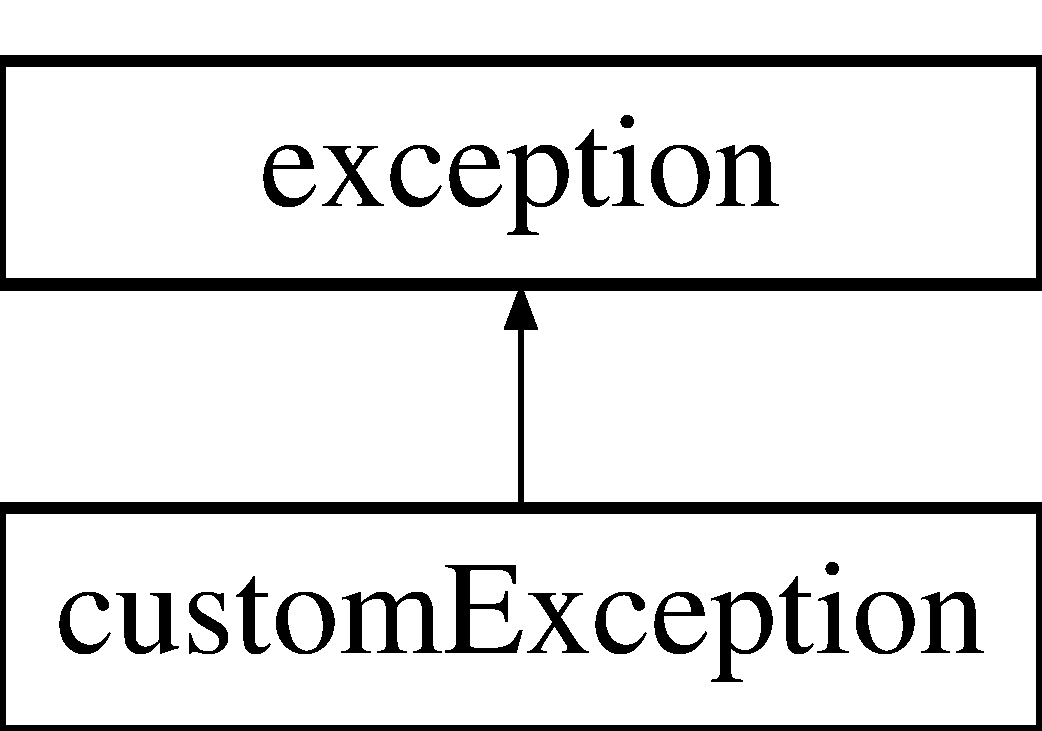
\includegraphics[height=2.000000cm]{classcustom_exception}
\end{center}
\end{figure}
\subsection*{Public Member Functions}
\begin{DoxyCompactItemize}
\item 
const char $\ast$ \hyperlink{classcustom_exception_aeb6ab5848b038adfc68fde86a512f691}{what} () const   throw ()
\begin{DoxyCompactList}\small\item\em Return the user's message. \end{DoxyCompactList}\item 
\hyperlink{classcustom_exception_a02ff9f09c4dd8c0b62fb1b6438d7d71a}{custom\-Exception} (std\-::string m=\char`\"{}custom exception occurred\char`\"{})
\begin{DoxyCompactList}\small\item\em Instantiate an exeption with a user-\/defined error message. \end{DoxyCompactList}\item 
\hyperlink{classcustom_exception_a361fad49d4068f3d5fe8d4a1a962791a}{$\sim$custom\-Exception} ()  throw ()
\begin{DoxyCompactList}\small\item\em Throw the message to the user. \end{DoxyCompactList}\end{DoxyCompactItemize}


\subsection{Detailed Description}
Error handling via custom exceptions. 

Definition at line 168 of file global.\-h.



\subsection{Constructor \& Destructor Documentation}
\hypertarget{classcustom_exception_a02ff9f09c4dd8c0b62fb1b6438d7d71a}{\index{custom\-Exception@{custom\-Exception}!custom\-Exception@{custom\-Exception}}
\index{custom\-Exception@{custom\-Exception}!customException@{custom\-Exception}}
\subsubsection[{custom\-Exception}]{\setlength{\rightskip}{0pt plus 5cm}custom\-Exception\-::custom\-Exception (
\begin{DoxyParamCaption}
\item[{std\-::string}]{m = {\ttfamily \char`\"{}custom~exception~occurred\char`\"{}}}
\end{DoxyParamCaption}
)\hspace{0.3cm}{\ttfamily [inline]}}}\label{classcustom_exception_a02ff9f09c4dd8c0b62fb1b6438d7d71a}


Instantiate an exeption with a user-\/defined error message. 



Definition at line 171 of file global.\-h.

\hypertarget{classcustom_exception_a361fad49d4068f3d5fe8d4a1a962791a}{\index{custom\-Exception@{custom\-Exception}!$\sim$custom\-Exception@{$\sim$custom\-Exception}}
\index{$\sim$custom\-Exception@{$\sim$custom\-Exception}!customException@{custom\-Exception}}
\subsubsection[{$\sim$custom\-Exception}]{\setlength{\rightskip}{0pt plus 5cm}custom\-Exception\-::$\sim$custom\-Exception (
\begin{DoxyParamCaption}
{}
\end{DoxyParamCaption}
) throw  ) \hspace{0.3cm}{\ttfamily [inline]}}}\label{classcustom_exception_a361fad49d4068f3d5fe8d4a1a962791a}


Throw the message to the user. 



Definition at line 172 of file global.\-h.



\subsection{Member Function Documentation}
\hypertarget{classcustom_exception_aeb6ab5848b038adfc68fde86a512f691}{\index{custom\-Exception@{custom\-Exception}!what@{what}}
\index{what@{what}!customException@{custom\-Exception}}
\subsubsection[{what}]{\setlength{\rightskip}{0pt plus 5cm}const char$\ast$ custom\-Exception\-::what (
\begin{DoxyParamCaption}
{}
\end{DoxyParamCaption}
) const throw  ) \hspace{0.3cm}{\ttfamily [inline]}}}\label{classcustom_exception_aeb6ab5848b038adfc68fde86a512f691}


Return the user's message. 



Definition at line 170 of file global.\-h.



Referenced by right\-Triangle\-X\-Z\-::inside(), agg\-Vol\-Bias3\-::make(), delete\-Particle\-::make(), translate\-Particle\-::make(), insert\-Particle\-::make(), swap\-Particles\-::make(), moves\-::make\-Move(), moves\-::moves(), perform\-Crossover(), perform\-T\-M\-M\-C(), perform\-W\-A\-L\-A(), sim\-System\-::read\-Config(), dynamic\-\_\-one\-\_\-dim\-\_\-histogram\-::record(), sim\-System\-::refine\-Energy\-Histogram\-Bounds(), sim\-System\-::restart\-Ext\-Moments(), sim\-System\-::scratch\-Energy(), set\-Barriers(), set\-Config(), sim\-System\-::start\-T\-M\-M\-C(), sim\-System\-::start\-W\-A\-L\-A(), and tmmc\-::update\-C().



The documentation for this class was generated from the following file\-:\begin{DoxyCompactItemize}
\item 
/home/nam4/\-Desktop/sandbox/\-F\-H\-M\-C\-Simulation/src/\hyperlink{global_8h}{global.\-h}\end{DoxyCompactItemize}

\hypertarget{classcylinder_z}{\section{cylinder\-Z Class Reference}
\label{classcylinder_z}\index{cylinder\-Z@{cylinder\-Z}}
}


Cylinder along z = 0 axis at a given (x,y) coordinate.  




{\ttfamily \#include $<$barrier.\-h$>$}

Inheritance diagram for cylinder\-Z\-:\begin{figure}[H]
\begin{center}
\leavevmode
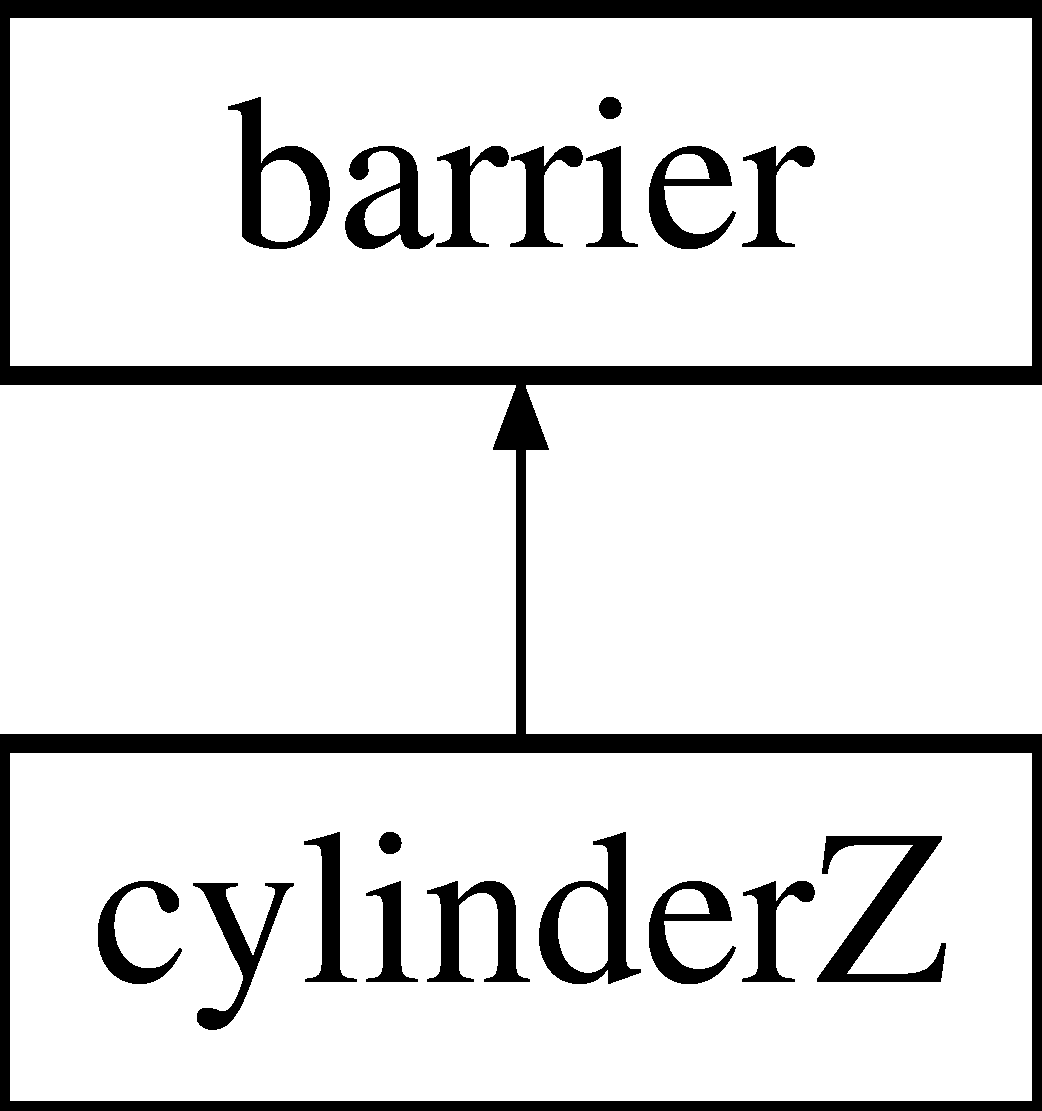
\includegraphics[height=2.000000cm]{classcylinder_z}
\end{center}
\end{figure}
\subsection*{Public Member Functions}
\begin{DoxyCompactItemize}
\item 
\hyperlink{classcylinder_z_a06f3ecc97023c1806d587f93a1c6c565}{$\sim$cylinder\-Z} ()
\item 
\hyperlink{classcylinder_z_a6891adbe87a6814239c8a143e996b1b0}{cylinder\-Z} (const double x, const double y, const double radius, const double width, const double sigma, const double eps, const int M=1)
\begin{DoxyCompactList}\small\item\em Instantiate a cylinderical pore in the z-\/direction. \end{DoxyCompactList}\item 
bool \hyperlink{classcylinder_z_aff84684096c1d04d73ee894b499a0a2f}{inside} (const \hyperlink{classatom}{atom} $\ast$a1, const std\-::vector$<$ double $>$ \&box)
\begin{DoxyCompactList}\small\item\em Return whether or not a point falls inside the cylinder (subject to a hard-\/sphere exclusion radius). \end{DoxyCompactList}\item 
double \hyperlink{classcylinder_z_a0d1ec094ac9bf23b74e6f03f09477217}{energy} (const \hyperlink{classatom}{atom} $\ast$a1, const std\-::vector$<$ double $>$ \&box)
\begin{DoxyCompactList}\small\item\em Interaction energy with the cylinder. \end{DoxyCompactList}\end{DoxyCompactItemize}
\subsection*{Additional Inherited Members}


\subsection{Detailed Description}
Cylinder along z = 0 axis at a given (x,y) coordinate. 

Definition at line 64 of file barrier.\-h.



\subsection{Constructor \& Destructor Documentation}
\hypertarget{classcylinder_z_a06f3ecc97023c1806d587f93a1c6c565}{\index{cylinder\-Z@{cylinder\-Z}!$\sim$cylinder\-Z@{$\sim$cylinder\-Z}}
\index{$\sim$cylinder\-Z@{$\sim$cylinder\-Z}!cylinderZ@{cylinder\-Z}}
\subsubsection[{$\sim$cylinder\-Z}]{\setlength{\rightskip}{0pt plus 5cm}cylinder\-Z\-::$\sim$cylinder\-Z (
\begin{DoxyParamCaption}
{}
\end{DoxyParamCaption}
)\hspace{0.3cm}{\ttfamily [inline]}}}\label{classcylinder_z_a06f3ecc97023c1806d587f93a1c6c565}


Definition at line 66 of file barrier.\-h.


\begin{DoxyCode}
66 \{\};
\end{DoxyCode}
\hypertarget{classcylinder_z_a6891adbe87a6814239c8a143e996b1b0}{\index{cylinder\-Z@{cylinder\-Z}!cylinder\-Z@{cylinder\-Z}}
\index{cylinder\-Z@{cylinder\-Z}!cylinderZ@{cylinder\-Z}}
\subsubsection[{cylinder\-Z}]{\setlength{\rightskip}{0pt plus 5cm}cylinder\-Z\-::cylinder\-Z (
\begin{DoxyParamCaption}
\item[{const double}]{x, }
\item[{const double}]{y, }
\item[{const double}]{radius, }
\item[{const double}]{width, }
\item[{const double}]{sigma, }
\item[{const double}]{eps, }
\item[{const int}]{M = {\ttfamily 1}}
\end{DoxyParamCaption}
)}}\label{classcylinder_z_a6891adbe87a6814239c8a143e996b1b0}


Instantiate a cylinderical pore in the z-\/direction. 

Expanded ensembles primarily scale the magnitude of interaction. The repulsive boundary scales with sigma at the boundary, but the attractive cutoff remains fixed relative to the boundary.


\begin{DoxyParams}[1]{Parameters}
\mbox{\tt in}  & {\em x} & x-\/coordinate of cylinder's center \\
\hline
\mbox{\tt in}  & {\em y} & y-\/coordinate of cylinder's center \\
\hline
\mbox{\tt in}  & {\em radius} & Radius of cylinder \\
\hline
\mbox{\tt in}  & {\em width} & Width of square-\/well-\/like interaction (distance from wall) \\
\hline
\mbox{\tt in}  & {\em sigma} & Hard-\/sphere diameter the species this wall interacts with can approach within \\
\hline
\mbox{\tt in}  & {\em eps} & Magnitude of the wall interaction (U = -\/eps) \\
\hline
\mbox{\tt in}  & {\em M} & Total number of expanded ensemble states possible for this atom type (defaults to 1) \\
\hline
\end{DoxyParams}


Definition at line 462 of file barrier.\-cpp.



References barrier\-::\-M\-\_\-.


\begin{DoxyCode}
462                                                                                                            
                                           \{
463     \textcolor{keywordflow}{if} (radius <= sigma) \{
464         \textcolor{keywordflow}{throw} \hyperlink{classcustom_exception}{customException} (\textcolor{stringliteral}{"cylinderZ radius <= sigma so practically no particles will
       fit"});
465     \}
466     \textcolor{keywordflow}{if} (sigma < 0) \{
467         \textcolor{keywordflow}{throw} \hyperlink{classcustom_exception}{customException} (\textcolor{stringliteral}{"cylinderZ must have sigma >= 0"});
468     \}
469     \textcolor{keywordflow}{if} (width < 0) \{
470         \textcolor{keywordflow}{throw} \hyperlink{classcustom_exception}{customException} (\textcolor{stringliteral}{"cylinderZ must have width >= 0"});
471     \}
472     \textcolor{keywordflow}{if} (eps < 0) \{
473         \textcolor{keywordflow}{throw} \hyperlink{classcustom_exception}{customException} (\textcolor{stringliteral}{"cylinderZ must have epsilon >= 0"});
474     \}
475     \textcolor{keywordflow}{if} (sigma/2.0 >= width) \{
476         \textcolor{keywordflow}{throw} \hyperlink{classcustom_exception}{customException} (\textcolor{stringliteral}{"cylinderZ must have sigma/2 < width to have a finite range
       of interaction"});
477     \}
478     \textcolor{keywordflow}{if} (M < 1) \{
479         \textcolor{keywordflow}{throw} \hyperlink{classcustom_exception}{customException} (\textcolor{stringliteral}{"cylinderZ must have M >= 1"});
480     \}
481 
482     eps\_ = eps;
483     sigma\_ = sigma;
484     width\_ = width;
485     radius\_ = radius;
486     \hyperlink{classbarrier_a274cf283ffc97c22ffa9a4258369c400}{M\_} = M;
487 
488     center\_.resize(3, 0);
489     center\_[0] = x;
490     center\_[1] = y;
491 \}
\end{DoxyCode}


\subsection{Member Function Documentation}
\hypertarget{classcylinder_z_a0d1ec094ac9bf23b74e6f03f09477217}{\index{cylinder\-Z@{cylinder\-Z}!energy@{energy}}
\index{energy@{energy}!cylinderZ@{cylinder\-Z}}
\subsubsection[{energy}]{\setlength{\rightskip}{0pt plus 5cm}double cylinder\-Z\-::energy (
\begin{DoxyParamCaption}
\item[{const {\bf atom} $\ast$}]{a1, }
\item[{const std\-::vector$<$ double $>$ \&}]{box}
\end{DoxyParamCaption}
)\hspace{0.3cm}{\ttfamily [virtual]}}}\label{classcylinder_z_a0d1ec094ac9bf23b74e6f03f09477217}


Interaction energy with the cylinder. 

Sigma and epsilon are scaled linearly with expanded ensemble state.


\begin{DoxyParams}[1]{Parameters}
\mbox{\tt in}  & {\em a1} & Pointer to atom with position to test -\/ this does N\-O\-T need to be in the simulation box a priori \\
\hline
\mbox{\tt in}  & {\em box} & Simulation box \\
\hline
\end{DoxyParams}


Implements \hyperlink{classbarrier_a2d308cfd5709aa479d0b37733f1a0db7}{barrier}.



Definition at line 525 of file barrier.\-cpp.



References barrier\-::\-M\-\_\-, atom\-::m\-State, N\-U\-M\-\_\-\-I\-N\-F\-I\-N\-I\-T\-Y, pbc\-Dist2(), and atom\-::pos.


\begin{DoxyCode}
525                                                                          \{
526     center\_[2] = a1->\hyperlink{classatom_a3ae5f4880e7831d8b2c9fda72b4eb24a}{pos}[2]; \textcolor{comment}{// same z-plane}
527     \textcolor{keywordtype}{double} rv2 = \hyperlink{utilities_8cpp_abb1db3a8a3ac46e044bbe7b2c5684c0a}{pbcDist2} (a1->\hyperlink{classatom_a3ae5f4880e7831d8b2c9fda72b4eb24a}{pos}, center\_, box);
528     \textcolor{keywordtype}{double} U = 0.0, sig = sigma\_, eps = eps\_;
529 
530     \textcolor{keywordflow}{if} (a1->\hyperlink{classatom_a3cb00c0c5b7533657e05af6ff4a42740}{mState} > 0) \{
531         sig = (sigma\_/\hyperlink{classbarrier_a274cf283ffc97c22ffa9a4258369c400}{M\_})*a1->\hyperlink{classatom_a3cb00c0c5b7533657e05af6ff4a42740}{mState};
532         eps = (eps\_/\hyperlink{classbarrier_a274cf283ffc97c22ffa9a4258369c400}{M\_})*a1->\hyperlink{classatom_a3cb00c0c5b7533657e05af6ff4a42740}{mState};
533     \}
534     \textcolor{keywordflow}{if} (a1->\hyperlink{classatom_a3cb00c0c5b7533657e05af6ff4a42740}{mState} < 0 || a1->\hyperlink{classatom_a3cb00c0c5b7533657e05af6ff4a42740}{mState} > \hyperlink{classbarrier_a274cf283ffc97c22ffa9a4258369c400}{M\_}-1) \{
535         \textcolor{keywordflow}{throw} \hyperlink{classcustom_exception}{customException} (\textcolor{stringliteral}{"mState out of bounds for cylinderZ"});
536     \}
537 
538     \textcolor{comment}{// Return infinity if out of bounds}
539     \textcolor{keywordtype}{double} rc = radius\_ - sig/2.0, ri = radius\_ - width\_;
540     \textcolor{keywordflow}{if} (rv2 >= rc*rc) \{
541         \textcolor{keywordflow}{return} \hyperlink{potentials_8h_ab94ab1d09e2291d03fe92a0e24a9d33b}{NUM\_INFINITY};
542     \}
543 
544     \textcolor{comment}{// Interaction with the wall - return infinity if it was out of bounds already}
545     \textcolor{keywordflow}{if} (rv2 > ri*ri) \{
546         U += -eps;
547     \}
548 
549     \textcolor{keywordflow}{return} U;
550 \}
\end{DoxyCode}
\hypertarget{classcylinder_z_aff84684096c1d04d73ee894b499a0a2f}{\index{cylinder\-Z@{cylinder\-Z}!inside@{inside}}
\index{inside@{inside}!cylinderZ@{cylinder\-Z}}
\subsubsection[{inside}]{\setlength{\rightskip}{0pt plus 5cm}bool cylinder\-Z\-::inside (
\begin{DoxyParamCaption}
\item[{const {\bf atom} $\ast$}]{a1, }
\item[{const std\-::vector$<$ double $>$ \&}]{box}
\end{DoxyParamCaption}
)\hspace{0.3cm}{\ttfamily [virtual]}}}\label{classcylinder_z_aff84684096c1d04d73ee894b499a0a2f}


Return whether or not a point falls inside the cylinder (subject to a hard-\/sphere exclusion radius). 

Sigma is scaled linearly with expanded ensemble state.


\begin{DoxyParams}[1]{Parameters}
\mbox{\tt in}  & {\em a1} & Pointer to atom with position to test -\/ this does N\-O\-T need to be in the simulation box a priori \\
\hline
\mbox{\tt in}  & {\em box} & Simulation box \\
\hline
\end{DoxyParams}


Implements \hyperlink{classbarrier_a948ebdcfac501cb75d1a1f045a7d9125}{barrier}.



Definition at line 499 of file barrier.\-cpp.



References barrier\-::\-M\-\_\-, atom\-::m\-State, pbc\-Dist2(), and atom\-::pos.


\begin{DoxyCode}
499                                                                        \{
500     center\_[2] = a1->\hyperlink{classatom_a3ae5f4880e7831d8b2c9fda72b4eb24a}{pos}[2]; \textcolor{comment}{// same z-plane}
501     \textcolor{keywordtype}{double} rv2 = \hyperlink{utilities_8cpp_abb1db3a8a3ac46e044bbe7b2c5684c0a}{pbcDist2} (a1->\hyperlink{classatom_a3ae5f4880e7831d8b2c9fda72b4eb24a}{pos}, center\_, box);
502 
503     \textcolor{keywordtype}{double} sig = sigma\_;
504     \textcolor{keywordflow}{if} (a1->\hyperlink{classatom_a3cb00c0c5b7533657e05af6ff4a42740}{mState} > 0) \{
505         sig = (sigma\_/\hyperlink{classbarrier_a274cf283ffc97c22ffa9a4258369c400}{M\_})*a1->\hyperlink{classatom_a3cb00c0c5b7533657e05af6ff4a42740}{mState};
506     \}
507     \textcolor{keywordflow}{if} (a1->\hyperlink{classatom_a3cb00c0c5b7533657e05af6ff4a42740}{mState} < 0 || a1->\hyperlink{classatom_a3cb00c0c5b7533657e05af6ff4a42740}{mState} > \hyperlink{classbarrier_a274cf283ffc97c22ffa9a4258369c400}{M\_}-1) \{
508         \textcolor{keywordflow}{throw} \hyperlink{classcustom_exception}{customException} (\textcolor{stringliteral}{"mState out of bounds for cylinderZ"});
509     \}
510 
511     \textcolor{keywordtype}{double} rc = radius\_ - sig/2.0;
512     \textcolor{keywordflow}{if} (rv2 >= rc*rc) \{
513         \textcolor{keywordflow}{return} \textcolor{keyword}{false};
514     \} \textcolor{keywordflow}{else} \{
515         \textcolor{keywordflow}{return} \textcolor{keyword}{true};
516     \}
517 \}
\end{DoxyCode}


The documentation for this class was generated from the following files\-:\begin{DoxyCompactItemize}
\item 
/home/nam4/\-Desktop/sandbox/\-F\-H\-M\-C\-Simulation/src/\hyperlink{barrier_8h}{barrier.\-h}\item 
/home/nam4/\-Desktop/sandbox/\-F\-H\-M\-C\-Simulation/src/\hyperlink{barrier_8cpp}{barrier.\-cpp}\end{DoxyCompactItemize}

\hypertarget{classdelete_particle}{}\section{delete\+Particle Class Reference}
\label{classdelete_particle}\index{delete\+Particle@{delete\+Particle}}


{\ttfamily \#include $<$delete.\+h$>$}

Inheritance diagram for delete\+Particle\+:\begin{figure}[H]
\begin{center}
\leavevmode
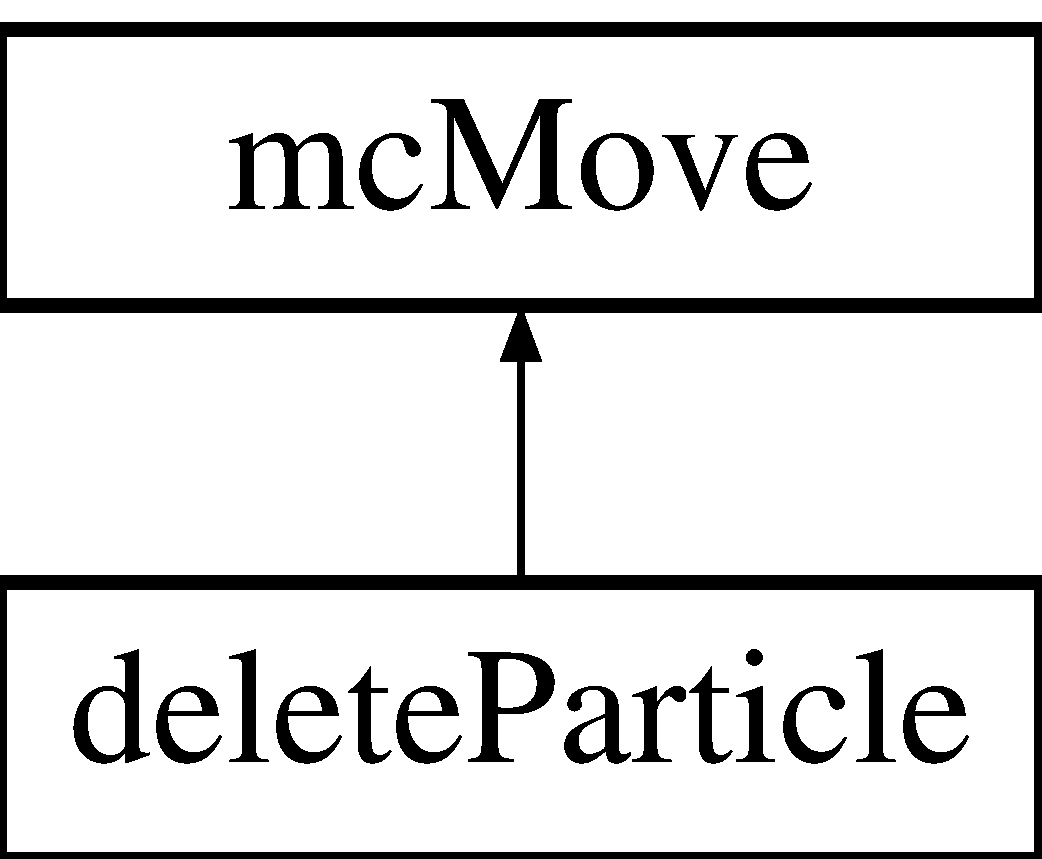
\includegraphics[height=2.000000cm]{classdelete_particle}
\end{center}
\end{figure}
\subsection*{Public Member Functions}
\begin{DoxyCompactItemize}
\item 
\hyperlink{classdelete_particle_a3b97ed18c7080043db26d2716c67dde0}{delete\+Particle} ()
\item 
\hyperlink{classdelete_particle_ae1a05ba703e5df3173384831fccc8698}{delete\+Particle} (const int type\+Index, const std\+::string tag)
\begin{DoxyCompactList}\small\item\em Instantiate a new move, also give a name which is the combination of auser-\/defined tag + the particle index it operates on. \end{DoxyCompactList}\item 
int \hyperlink{classdelete_particle_a14f86dd27a82f571caa12af04e22eb1f}{make} (\hyperlink{classsim_system}{sim\+System} \&sys)
\begin{DoxyCompactList}\small\item\em Delete a particle from the system. \end{DoxyCompactList}\end{DoxyCompactItemize}
\subsection*{Additional Inherited Members}


\subsection{Detailed Description}


Definition at line 12 of file delete.\+h.



\subsection{Constructor \& Destructor Documentation}
\hypertarget{classdelete_particle_a3b97ed18c7080043db26d2716c67dde0}{}\index{delete\+Particle@{delete\+Particle}!delete\+Particle@{delete\+Particle}}
\index{delete\+Particle@{delete\+Particle}!delete\+Particle@{delete\+Particle}}
\subsubsection[{delete\+Particle()}]{\setlength{\rightskip}{0pt plus 5cm}delete\+Particle\+::delete\+Particle (
\begin{DoxyParamCaption}
{}
\end{DoxyParamCaption}
)\hspace{0.3cm}{\ttfamily [inline]}}\label{classdelete_particle_a3b97ed18c7080043db26d2716c67dde0}


Definition at line 14 of file delete.\+h.


\begin{DoxyCode}
14 \{\};
\end{DoxyCode}
\hypertarget{classdelete_particle_ae1a05ba703e5df3173384831fccc8698}{}\index{delete\+Particle@{delete\+Particle}!delete\+Particle@{delete\+Particle}}
\index{delete\+Particle@{delete\+Particle}!delete\+Particle@{delete\+Particle}}
\subsubsection[{delete\+Particle(const int type\+Index, const std\+::string tag)}]{\setlength{\rightskip}{0pt plus 5cm}delete\+Particle\+::delete\+Particle (
\begin{DoxyParamCaption}
\item[{const int}]{type\+Index, }
\item[{const std\+::string}]{tag}
\end{DoxyParamCaption}
)\hspace{0.3cm}{\ttfamily [inline]}}\label{classdelete_particle_ae1a05ba703e5df3173384831fccc8698}


Instantiate a new move, also give a name which is the combination of auser-\/defined tag + the particle index it operates on. 



Definition at line 15 of file delete.\+h.



References mc\+Move\+::name\+\_\+, and mc\+Move\+::type\+Index\+\_\+.



\subsection{Member Function Documentation}
\hypertarget{classdelete_particle_a14f86dd27a82f571caa12af04e22eb1f}{}\index{delete\+Particle@{delete\+Particle}!make@{make}}
\index{make@{make}!delete\+Particle@{delete\+Particle}}
\subsubsection[{make(sim\+System \&sys)}]{\setlength{\rightskip}{0pt plus 5cm}int delete\+Particle\+::make (
\begin{DoxyParamCaption}
\item[{{\bf sim\+System} \&}]{sys}
\end{DoxyParamCaption}
)\hspace{0.3cm}{\ttfamily [virtual]}}\label{classdelete_particle_a14f86dd27a82f571caa12af04e22eb1f}


Delete a particle from the system. 

All other information is stored in the \hyperlink{classsim_system}{sim\+System} object.


\begin{DoxyParams}[1]{Parameters}
\mbox{\tt in}  & {\em sys} & System object to attempt to remove a particle from.\\
\hline
\end{DoxyParams}
\begin{DoxyReturn}{Returns}
M\+O\+V\+E\+\_\+\+S\+U\+C\+C\+E\+S\+S if deleted a particle, otherwise M\+O\+V\+E\+\_\+\+F\+A\+I\+L\+U\+R\+E if did not. Will throw exceptions if there was an error. 
\end{DoxyReturn}


Implements \hyperlink{classmc_move_a2e377a628f9ecee5422fc8967d4924eb}{mc\+Move}.



Definition at line 10 of file delete.\+cpp.



References sim\+System\+::atoms, sim\+System\+::beta(), sim\+System\+::box(), calculate\+Bias(), sim\+System\+::delete\+Atom(), sim\+System\+::get\+Neighbor\+Positions(), sim\+System\+::get\+Tot\+N(), sim\+System\+::get\+W\+A\+L\+A\+Bias(), sim\+System\+::increment\+Energy(), sim\+System\+::min\+Species(), M\+O\+V\+E\+\_\+\+F\+A\+I\+L\+U\+R\+E, M\+O\+V\+E\+\_\+\+S\+U\+C\+C\+E\+S\+S, sim\+System\+::mu(), sim\+System\+::n\+Species(), sim\+System\+::num\+Species, sim\+System\+::ppot, rng(), R\+N\+G\+\_\+\+S\+E\+E\+D, sim\+System\+::tot\+N\+Min(), mc\+Move\+::type\+Index\+\_\+, wala\+::update(), sim\+System\+::use\+W\+A\+L\+A, and custom\+Exception\+::what().


\begin{DoxyCode}
10                                         \{
11                 \textcolor{comment}{// check if any can be deleted from this species}
12     \textcolor{keywordflow}{if} (sys.\hyperlink{classsim_system_a9eea865e6dc1cff377b1e79c4d9c23f0}{numSpecies}[\hyperlink{classmc_move_acb731965547b0326ef318ec96da8b46a}{typeIndex\_}] <= sys.\hyperlink{classsim_system_afafda4a09ed180ee9c5580d196d8ca9f}{minSpecies}(
      \hyperlink{classmc_move_acb731965547b0326ef318ec96da8b46a}{typeIndex\_})) \{
13         \textcolor{keywordflow}{return} \hyperlink{moves_8h_a9832cf5fcfa8c0894545b591c9908e39}{MOVE\_FAILURE};
14     \}
15     \textcolor{comment}{// also check if at global bound on total number of particles}
16     \textcolor{keywordflow}{if} (sys.\hyperlink{classsim_system_a37dd827f4057049763351510147b9f1d}{getTotN}() <= sys.\hyperlink{classsim_system_af10842e0eaa638373b8717c87b47e6bc}{totNMin}()) \{
17                 \textcolor{keywordflow}{return} \hyperlink{moves_8h_a9832cf5fcfa8c0894545b591c9908e39}{MOVE\_FAILURE};
18     \}
19     
20                 \textcolor{comment}{// choose a random particle (index) of that type}
21                 \textcolor{keyword}{const} \textcolor{keywordtype}{int} chosenAtom = (int) floor(\hyperlink{utilities_8cpp_a0f9542af4b475ac79cb679d7a8d14db0}{rng} (&\hyperlink{global_8h_a3f4e4ea24d5a5c66feae55d1f329c884}{RNG\_SEED}) * sys.
      \hyperlink{classsim_system_a9eea865e6dc1cff377b1e79c4d9c23f0}{numSpecies}[\hyperlink{classmc_move_acb731965547b0326ef318ec96da8b46a}{typeIndex\_}]);
22 
23                 \textcolor{comment}{// attempt to delete that one}
24                 \textcolor{keyword}{const} std::vector < double > box = sys.\hyperlink{classsim_system_a8bff9dfb95b1b09a0fab2c1c485ade07}{box}();
25     \textcolor{keywordtype}{double} V = 1.0;
26     \textcolor{keywordflow}{for} (\textcolor{keywordtype}{unsigned} \textcolor{keywordtype}{int} i = 0; i < box.size(); ++i) \{
27         V *= box[i];
28     \}
29         
30     \textcolor{keywordtype}{double} delEnergy = 0.0;
31     \textcolor{keywordflow}{for} (\textcolor{keywordtype}{unsigned} \textcolor{keywordtype}{int} spec = 0; spec < sys.\hyperlink{classsim_system_ab5e2e9b6204de15520302fe1d51688dd}{nSpecies}(); ++spec) \{
32         \textcolor{comment}{// get positions of neighboring atoms around chosenAtom}
33         std::vector < std::vector< double > > neighborPositions = sys.
      \hyperlink{classsim_system_a7ac49b2311cd8230df8d078a9d897b35}{getNeighborPositions}(spec, \hyperlink{classmc_move_acb731965547b0326ef318ec96da8b46a}{typeIndex\_}, &sys.\hyperlink{classsim_system_a90421b19082f7fb8fc23b7264b1161e4}{atoms}[
      \hyperlink{classmc_move_acb731965547b0326ef318ec96da8b46a}{typeIndex\_}][chosenAtom]);
34         \textcolor{keywordflow}{for} (\textcolor{keywordtype}{unsigned} \textcolor{keywordtype}{int} i = 0; i < neighborPositions.size(); ++i) \{
35             \textcolor{keywordflow}{try} \{
36                                                                 delEnergy -= sys.
      \hyperlink{classsim_system_a8d6271751a62f61edcf57f773540a4a3}{ppot}[spec][\hyperlink{classmc_move_acb731965547b0326ef318ec96da8b46a}{typeIndex\_}]->energy(neighborPositions[i], sys.\hyperlink{classsim_system_a90421b19082f7fb8fc23b7264b1161e4}{atoms}[
      \hyperlink{classmc_move_acb731965547b0326ef318ec96da8b46a}{typeIndex\_}][chosenAtom].pos, box);
37                                                 \}
38                                                 \textcolor{keywordflow}{catch} (\hyperlink{classcustom_exception}{customException}& ce) \{
39                                                                 std::string a = \textcolor{stringliteral}{"Cannot delete because of
       energy error: "}, b = ce.\hyperlink{classcustom_exception_aeb6ab5848b038adfc68fde86a512f691}{what}();
40                                                                 \textcolor{keywordflow}{throw} 
      \hyperlink{classcustom_exception}{customException} (a+b);
41                                                 \}
42         \}
43         \textcolor{comment}{// add tail correction to potential energy -- only enable for fluid phase simulations}
44 \textcolor{preprocessor}{#ifdef FLUID\_PHASE\_SIMULATIONS}
45         \textcolor{keywordflow}{if} (sys.\hyperlink{classsim_system_a8d6271751a62f61edcf57f773540a4a3}{ppot}[spec][\hyperlink{classmc_move_acb731965547b0326ef318ec96da8b46a}{typeIndex\_}]->useTailCorrection) \{
46                 \textcolor{keywordflow}{if} (spec == typeIndex\_) \{
47                                                                 delEnergy -= sys.
      \hyperlink{classsim_system_a8d6271751a62f61edcf57f773540a4a3}{ppot}[spec][\hyperlink{classmc_move_acb731965547b0326ef318ec96da8b46a}{typeIndex\_}]->tailCorrection((sys.\hyperlink{classsim_system_a9eea865e6dc1cff377b1e79c4d9c23f0}{numSpecies}[spec]-1)/V);
48                                                 \}
49                                                 \textcolor{keywordflow}{else} \{
50                                                                 delEnergy -= sys.
      \hyperlink{classsim_system_a8d6271751a62f61edcf57f773540a4a3}{ppot}[spec][\hyperlink{classmc_move_acb731965547b0326ef318ec96da8b46a}{typeIndex\_}]->tailCorrection((sys.\hyperlink{classsim_system_a9eea865e6dc1cff377b1e79c4d9c23f0}{numSpecies}[spec])/V);
51                                                 \}
52                                 \}
53 \textcolor{preprocessor}{#endif}
54     \}
55     
56     \textcolor{comment}{// biasing}
57     \textcolor{keyword}{const} \textcolor{keywordtype}{double} p\_u = sys.\hyperlink{classsim_system_a9eea865e6dc1cff377b1e79c4d9c23f0}{numSpecies}[\hyperlink{classmc_move_acb731965547b0326ef318ec96da8b46a}{typeIndex\_}]/V*exp(sys.
      \hyperlink{classsim_system_a3eeec9678902f8d7fce4dad6064aaf4c}{beta}()*(-sys.\hyperlink{classsim_system_af1e3f5320aff976a448647244d5950d1}{mu}(typeIndex\_) - delEnergy));
58     \textcolor{keywordtype}{int} nTotFinal = sys.\hyperlink{classsim_system_a37dd827f4057049763351510147b9f1d}{getTotN}() - 1;
59     \textcolor{keywordtype}{double} bias = \hyperlink{system_8cpp_ab912bbb9fc9045954cf1b3ccb286a55c}{calculateBias}(sys, nTotFinal, p\_u);
60     
61                 \textcolor{comment}{// metropolis criterion}
62                 \textcolor{keywordflow}{if} (\hyperlink{utilities_8cpp_a0f9542af4b475ac79cb679d7a8d14db0}{rng} (&\hyperlink{global_8h_a3f4e4ea24d5a5c66feae55d1f329c884}{RNG\_SEED}) < p\_u*bias) \{
63                     \textcolor{keywordflow}{try} \{
64             sys.\hyperlink{classsim_system_acabf4fc5b5b90bba62e1449ddb3646c6}{deleteAtom}(typeIndex\_, chosenAtom);
65         \} \textcolor{keywordflow}{catch} (\hyperlink{classcustom_exception}{customException} &ce) \{
66             std::string a = \textcolor{stringliteral}{"Failed to delete atom: "}, b = ce.\hyperlink{classcustom_exception_aeb6ab5848b038adfc68fde86a512f691}{what}();
67             \textcolor{keywordflow}{throw} \hyperlink{classcustom_exception}{customException} (a+b);
68         \}
69                                 sys.\hyperlink{classsim_system_a6ad31c08955b80873f865b3069618dcb}{incrementEnergy}(delEnergy);  
70                                 
71                                 \textcolor{comment}{// update Wang-Landau bias, if used}
72                                 \textcolor{keywordflow}{if} (sys.\hyperlink{classsim_system_aa83b00006b3919fb6e13f1bdeadece6a}{useWALA}) \{
73                                                 sys.\hyperlink{classsim_system_a7cb5049de8b0988349e89e30e4000407}{getWALABias}()->
      \hyperlink{classwala_a5eb2622be6a9e89f5e59ba0b15aca4bd}{update}(sys.\hyperlink{classsim_system_a37dd827f4057049763351510147b9f1d}{getTotN}());
74                                 \}
75                                                                 
76         \textcolor{keywordflow}{return} \hyperlink{moves_8h_ae8285cbddc5d21f73f49dcbad82a775a}{MOVE\_SUCCESS};
77     \}
78     
79                 \textcolor{comment}{// update Wang-Landau bias (even if moved failed), if used}
80                 \textcolor{keywordflow}{if} (sys.\hyperlink{classsim_system_aa83b00006b3919fb6e13f1bdeadece6a}{useWALA}) \{
81                                 sys.\hyperlink{classsim_system_a7cb5049de8b0988349e89e30e4000407}{getWALABias}()->\hyperlink{classwala_a5eb2622be6a9e89f5e59ba0b15aca4bd}{update}(sys.
      \hyperlink{classsim_system_a37dd827f4057049763351510147b9f1d}{getTotN}());
82                 \}
83                                 
84                 \textcolor{keywordflow}{return} \hyperlink{moves_8h_a9832cf5fcfa8c0894545b591c9908e39}{MOVE\_FAILURE};
85 \}
\end{DoxyCode}


The documentation for this class was generated from the following files\+:\begin{DoxyCompactItemize}
\item 
/\+Users/nam4/\+Desktop/omcs/src/\hyperlink{delete_8h}{delete.\+h}\item 
/\+Users/nam4/\+Desktop/omcs/src/\hyperlink{delete_8cpp}{delete.\+cpp}\end{DoxyCompactItemize}

\hypertarget{classdynamic__one__dim__histogram}{\section{dynamic\-\_\-one\-\_\-dim\-\_\-histogram Class Reference}
\label{classdynamic__one__dim__histogram}\index{dynamic\-\_\-one\-\_\-dim\-\_\-histogram@{dynamic\-\_\-one\-\_\-dim\-\_\-histogram}}
}


{\ttfamily \#include $<$histogram.\-h$>$}

\subsection*{Public Member Functions}
\begin{DoxyCompactItemize}
\item 
\hyperlink{classdynamic__one__dim__histogram_a23aed9a23459cdee64422347878d81af}{$\sim$dynamic\-\_\-one\-\_\-dim\-\_\-histogram} ()
\item 
\hyperlink{classdynamic__one__dim__histogram_a361db85e9c1b246c24c4fdcba934de08}{dynamic\-\_\-one\-\_\-dim\-\_\-histogram} ()
\item 
\hyperlink{classdynamic__one__dim__histogram_a5c11c62055bece5d5bce48c27e8d8f99}{dynamic\-\_\-one\-\_\-dim\-\_\-histogram} (const double lb, const double ub, const double delta)
\begin{DoxyCompactList}\small\item\em Instantiate a 1\-D histogram that grow as needed to record values. \end{DoxyCompactList}\item 
void \hyperlink{classdynamic__one__dim__histogram_a899b4d0ab90f83506d12bc00c88a060a}{reinitialize} (const double lb, const double ub, const double delta)
\begin{DoxyCompactList}\small\item\em Re-\/initialize histogram and its bounds. \end{DoxyCompactList}\item 
void \hyperlink{classdynamic__one__dim__histogram_af03dc61101ae9d08b6f3474af04fbeeb}{trim\-\_\-edges} ()
\begin{DoxyCompactList}\small\item\em Trim the size of the histogram to remove leading and trailing zeros. \end{DoxyCompactList}\item 
void \hyperlink{classdynamic__one__dim__histogram_a03402a7219e10240803609fb6cbb24a6}{prepend\-\_\-bins} (const unsigned int nbins)
\begin{DoxyCompactList}\small\item\em Add a number of bins to the beginning of the histogram. \end{DoxyCompactList}\item 
void \hyperlink{classdynamic__one__dim__histogram_a6fa516279d227e363aa90baf29f8a181}{append\-\_\-bins} (const unsigned int nbins)
\begin{DoxyCompactList}\small\item\em Add a number of bins to the end of the histogram. \end{DoxyCompactList}\item 
void \hyperlink{classdynamic__one__dim__histogram_a2ae28c147c2dfc624ece9102603dd667}{record} (const double value)
\begin{DoxyCompactList}\small\item\em Record an entry in the histogram at the bin corresponding to where value falls. \end{DoxyCompactList}\item 
void \hyperlink{classdynamic__one__dim__histogram_a6fe82d8d8f463c6ca684bf1fead1d5c3}{set\-\_\-hist} (const std\-::deque$<$ double $>$ h)
\begin{DoxyCompactList}\small\item\em Set the histogram. \end{DoxyCompactList}\item 
const double \hyperlink{classdynamic__one__dim__histogram_a36567635816c1d33b8fb6f14ac50d575}{get\-\_\-delta} ()
\item 
const double \hyperlink{classdynamic__one__dim__histogram_a3849f19cd0c77e153cf32b0acefacc4d}{get\-\_\-lb} ()
\item 
const double \hyperlink{classdynamic__one__dim__histogram_a50871ffa445bce5f4443770a18db84aa}{get\-\_\-ub} ()
\item 
std\-::deque$<$ double $>$ \hyperlink{classdynamic__one__dim__histogram_ac3903fa9339e78a5b9abe908af279b0a}{get\-\_\-hist} ()
\end{DoxyCompactItemize}


\subsection{Detailed Description}


Definition at line 40 of file histogram.\-h.



\subsection{Constructor \& Destructor Documentation}
\hypertarget{classdynamic__one__dim__histogram_a23aed9a23459cdee64422347878d81af}{\index{dynamic\-\_\-one\-\_\-dim\-\_\-histogram@{dynamic\-\_\-one\-\_\-dim\-\_\-histogram}!$\sim$dynamic\-\_\-one\-\_\-dim\-\_\-histogram@{$\sim$dynamic\-\_\-one\-\_\-dim\-\_\-histogram}}
\index{$\sim$dynamic\-\_\-one\-\_\-dim\-\_\-histogram@{$\sim$dynamic\-\_\-one\-\_\-dim\-\_\-histogram}!dynamic_one_dim_histogram@{dynamic\-\_\-one\-\_\-dim\-\_\-histogram}}
\subsubsection[{$\sim$dynamic\-\_\-one\-\_\-dim\-\_\-histogram}]{\setlength{\rightskip}{0pt plus 5cm}dynamic\-\_\-one\-\_\-dim\-\_\-histogram\-::$\sim$dynamic\-\_\-one\-\_\-dim\-\_\-histogram (
\begin{DoxyParamCaption}
{}
\end{DoxyParamCaption}
)\hspace{0.3cm}{\ttfamily [inline]}}}\label{classdynamic__one__dim__histogram_a23aed9a23459cdee64422347878d81af}


Definition at line 42 of file histogram.\-h.


\begin{DoxyCode}
42 \{;\}
\end{DoxyCode}
\hypertarget{classdynamic__one__dim__histogram_a361db85e9c1b246c24c4fdcba934de08}{\index{dynamic\-\_\-one\-\_\-dim\-\_\-histogram@{dynamic\-\_\-one\-\_\-dim\-\_\-histogram}!dynamic\-\_\-one\-\_\-dim\-\_\-histogram@{dynamic\-\_\-one\-\_\-dim\-\_\-histogram}}
\index{dynamic\-\_\-one\-\_\-dim\-\_\-histogram@{dynamic\-\_\-one\-\_\-dim\-\_\-histogram}!dynamic_one_dim_histogram@{dynamic\-\_\-one\-\_\-dim\-\_\-histogram}}
\subsubsection[{dynamic\-\_\-one\-\_\-dim\-\_\-histogram}]{\setlength{\rightskip}{0pt plus 5cm}dynamic\-\_\-one\-\_\-dim\-\_\-histogram\-::dynamic\-\_\-one\-\_\-dim\-\_\-histogram (
\begin{DoxyParamCaption}
{}
\end{DoxyParamCaption}
)\hspace{0.3cm}{\ttfamily [inline]}}}\label{classdynamic__one__dim__histogram_a361db85e9c1b246c24c4fdcba934de08}


Definition at line 43 of file histogram.\-h.


\begin{DoxyCode}
43 \{;\}
\end{DoxyCode}
\hypertarget{classdynamic__one__dim__histogram_a5c11c62055bece5d5bce48c27e8d8f99}{\index{dynamic\-\_\-one\-\_\-dim\-\_\-histogram@{dynamic\-\_\-one\-\_\-dim\-\_\-histogram}!dynamic\-\_\-one\-\_\-dim\-\_\-histogram@{dynamic\-\_\-one\-\_\-dim\-\_\-histogram}}
\index{dynamic\-\_\-one\-\_\-dim\-\_\-histogram@{dynamic\-\_\-one\-\_\-dim\-\_\-histogram}!dynamic_one_dim_histogram@{dynamic\-\_\-one\-\_\-dim\-\_\-histogram}}
\subsubsection[{dynamic\-\_\-one\-\_\-dim\-\_\-histogram}]{\setlength{\rightskip}{0pt plus 5cm}dynamic\-\_\-one\-\_\-dim\-\_\-histogram\-::dynamic\-\_\-one\-\_\-dim\-\_\-histogram (
\begin{DoxyParamCaption}
\item[{const double}]{lb, }
\item[{const double}]{ub, }
\item[{const double}]{delta}
\end{DoxyParamCaption}
)}}\label{classdynamic__one__dim__histogram_a5c11c62055bece5d5bce48c27e8d8f99}


Instantiate a 1\-D histogram that grow as needed to record values. 

A bin is considered \char`\"{}centered\char`\"{} on its value.


\begin{DoxyParams}[1]{Parameters}
\mbox{\tt in}  & {\em lb} & Lower bound \\
\hline
\mbox{\tt in}  & {\em ub} & Upper bound \\
\hline
\mbox{\tt in}  & {\em delta} & Bin width \\
\hline
\end{DoxyParams}


Definition at line 99 of file histogram.\-cpp.


\begin{DoxyCode}
99                                                                                                           \{
100     \textcolor{keywordflow}{try} \{
101         initialize\_ (lb, ub, delta);
102     \} \textcolor{keywordflow}{catch} (\hyperlink{classcustom_exception}{customException} &ce) \{
103         \textcolor{keywordflow}{throw} \hyperlink{classcustom_exception}{customException} (\textcolor{stringliteral}{"Unable to initialize dynamic\_one\_dim\_histogram"});
104     \}
105 \}
\end{DoxyCode}


\subsection{Member Function Documentation}
\hypertarget{classdynamic__one__dim__histogram_a6fa516279d227e363aa90baf29f8a181}{\index{dynamic\-\_\-one\-\_\-dim\-\_\-histogram@{dynamic\-\_\-one\-\_\-dim\-\_\-histogram}!append\-\_\-bins@{append\-\_\-bins}}
\index{append\-\_\-bins@{append\-\_\-bins}!dynamic_one_dim_histogram@{dynamic\-\_\-one\-\_\-dim\-\_\-histogram}}
\subsubsection[{append\-\_\-bins}]{\setlength{\rightskip}{0pt plus 5cm}void dynamic\-\_\-one\-\_\-dim\-\_\-histogram\-::append\-\_\-bins (
\begin{DoxyParamCaption}
\item[{const unsigned int}]{nbins}
\end{DoxyParamCaption}
)}}\label{classdynamic__one__dim__histogram_a6fa516279d227e363aa90baf29f8a181}


Add a number of bins to the end of the histogram. 


\begin{DoxyParams}[1]{Parameters}
\mbox{\tt in}  & {\em nbins} & Number of bins to add to the end \\
\hline
\end{DoxyParams}


Definition at line 129 of file histogram.\-cpp.



Referenced by record().


\begin{DoxyCode}
129                                                                      \{
130     \textcolor{keywordflow}{for} (\textcolor{keywordtype}{unsigned} \textcolor{keywordtype}{int} i = 0; i < nbins; i++) \{
131         \textcolor{keywordflow}{try} \{
132             h\_.push\_back (0.0);
133             nbins\_++;
134             ub\_ += delta\_;
135         \} \textcolor{keywordflow}{catch} (std::bad\_alloc &ba) \{
136             \textcolor{keywordflow}{throw} \hyperlink{classcustom_exception}{customException} (\textcolor{stringliteral}{"Out of memory for dynamic\_one\_dim\_histogram"});
137         \}
138     \}
139 \}
\end{DoxyCode}
\hypertarget{classdynamic__one__dim__histogram_a36567635816c1d33b8fb6f14ac50d575}{\index{dynamic\-\_\-one\-\_\-dim\-\_\-histogram@{dynamic\-\_\-one\-\_\-dim\-\_\-histogram}!get\-\_\-delta@{get\-\_\-delta}}
\index{get\-\_\-delta@{get\-\_\-delta}!dynamic_one_dim_histogram@{dynamic\-\_\-one\-\_\-dim\-\_\-histogram}}
\subsubsection[{get\-\_\-delta}]{\setlength{\rightskip}{0pt plus 5cm}const double dynamic\-\_\-one\-\_\-dim\-\_\-histogram\-::get\-\_\-delta (
\begin{DoxyParamCaption}
{}
\end{DoxyParamCaption}
)\hspace{0.3cm}{\ttfamily [inline]}}}\label{classdynamic__one__dim__histogram_a36567635816c1d33b8fb6f14ac50d575}


Definition at line 52 of file histogram.\-h.


\begin{DoxyCode}
52 \{ \textcolor{keywordflow}{return} delta\_; \}
\end{DoxyCode}
\hypertarget{classdynamic__one__dim__histogram_ac3903fa9339e78a5b9abe908af279b0a}{\index{dynamic\-\_\-one\-\_\-dim\-\_\-histogram@{dynamic\-\_\-one\-\_\-dim\-\_\-histogram}!get\-\_\-hist@{get\-\_\-hist}}
\index{get\-\_\-hist@{get\-\_\-hist}!dynamic_one_dim_histogram@{dynamic\-\_\-one\-\_\-dim\-\_\-histogram}}
\subsubsection[{get\-\_\-hist}]{\setlength{\rightskip}{0pt plus 5cm}std\-::deque$<$ double $>$ dynamic\-\_\-one\-\_\-dim\-\_\-histogram\-::get\-\_\-hist (
\begin{DoxyParamCaption}
{}
\end{DoxyParamCaption}
)\hspace{0.3cm}{\ttfamily [inline]}}}\label{classdynamic__one__dim__histogram_ac3903fa9339e78a5b9abe908af279b0a}


Definition at line 55 of file histogram.\-h.


\begin{DoxyCode}
55 \{ \textcolor{keywordflow}{return} h\_; \}
\end{DoxyCode}
\hypertarget{classdynamic__one__dim__histogram_a3849f19cd0c77e153cf32b0acefacc4d}{\index{dynamic\-\_\-one\-\_\-dim\-\_\-histogram@{dynamic\-\_\-one\-\_\-dim\-\_\-histogram}!get\-\_\-lb@{get\-\_\-lb}}
\index{get\-\_\-lb@{get\-\_\-lb}!dynamic_one_dim_histogram@{dynamic\-\_\-one\-\_\-dim\-\_\-histogram}}
\subsubsection[{get\-\_\-lb}]{\setlength{\rightskip}{0pt plus 5cm}const double dynamic\-\_\-one\-\_\-dim\-\_\-histogram\-::get\-\_\-lb (
\begin{DoxyParamCaption}
{}
\end{DoxyParamCaption}
)\hspace{0.3cm}{\ttfamily [inline]}}}\label{classdynamic__one__dim__histogram_a3849f19cd0c77e153cf32b0acefacc4d}


Definition at line 53 of file histogram.\-h.


\begin{DoxyCode}
53 \{ \textcolor{keywordflow}{return} lb\_; \}
\end{DoxyCode}
\hypertarget{classdynamic__one__dim__histogram_a50871ffa445bce5f4443770a18db84aa}{\index{dynamic\-\_\-one\-\_\-dim\-\_\-histogram@{dynamic\-\_\-one\-\_\-dim\-\_\-histogram}!get\-\_\-ub@{get\-\_\-ub}}
\index{get\-\_\-ub@{get\-\_\-ub}!dynamic_one_dim_histogram@{dynamic\-\_\-one\-\_\-dim\-\_\-histogram}}
\subsubsection[{get\-\_\-ub}]{\setlength{\rightskip}{0pt plus 5cm}const double dynamic\-\_\-one\-\_\-dim\-\_\-histogram\-::get\-\_\-ub (
\begin{DoxyParamCaption}
{}
\end{DoxyParamCaption}
)\hspace{0.3cm}{\ttfamily [inline]}}}\label{classdynamic__one__dim__histogram_a50871ffa445bce5f4443770a18db84aa}


Definition at line 54 of file histogram.\-h.


\begin{DoxyCode}
54 \{ \textcolor{keywordflow}{return} ub\_; \}
\end{DoxyCode}
\hypertarget{classdynamic__one__dim__histogram_a03402a7219e10240803609fb6cbb24a6}{\index{dynamic\-\_\-one\-\_\-dim\-\_\-histogram@{dynamic\-\_\-one\-\_\-dim\-\_\-histogram}!prepend\-\_\-bins@{prepend\-\_\-bins}}
\index{prepend\-\_\-bins@{prepend\-\_\-bins}!dynamic_one_dim_histogram@{dynamic\-\_\-one\-\_\-dim\-\_\-histogram}}
\subsubsection[{prepend\-\_\-bins}]{\setlength{\rightskip}{0pt plus 5cm}void dynamic\-\_\-one\-\_\-dim\-\_\-histogram\-::prepend\-\_\-bins (
\begin{DoxyParamCaption}
\item[{const unsigned int}]{nbins}
\end{DoxyParamCaption}
)}}\label{classdynamic__one__dim__histogram_a03402a7219e10240803609fb6cbb24a6}


Add a number of bins to the beginning of the histogram. 


\begin{DoxyParams}[1]{Parameters}
\mbox{\tt in}  & {\em nbins} & Number of bins to add to the beginning \\
\hline
\end{DoxyParams}


Definition at line 112 of file histogram.\-cpp.



Referenced by record().


\begin{DoxyCode}
112                                                                       \{
113     \textcolor{keywordflow}{for} (\textcolor{keywordtype}{unsigned} \textcolor{keywordtype}{int} i = 0; i < nbins; i++) \{
114         \textcolor{keywordflow}{try} \{
115             h\_.push\_front (0.0);
116             nbins\_++;
117             lb\_ -= delta\_;
118         \} \textcolor{keywordflow}{catch} (std::bad\_alloc &ba) \{
119             \textcolor{keywordflow}{throw} \hyperlink{classcustom_exception}{customException} (\textcolor{stringliteral}{"Out of memory for dynamic\_one\_dim\_histogram"});
120         \}
121     \}
122 \}
\end{DoxyCode}
\hypertarget{classdynamic__one__dim__histogram_a2ae28c147c2dfc624ece9102603dd667}{\index{dynamic\-\_\-one\-\_\-dim\-\_\-histogram@{dynamic\-\_\-one\-\_\-dim\-\_\-histogram}!record@{record}}
\index{record@{record}!dynamic_one_dim_histogram@{dynamic\-\_\-one\-\_\-dim\-\_\-histogram}}
\subsubsection[{record}]{\setlength{\rightskip}{0pt plus 5cm}void dynamic\-\_\-one\-\_\-dim\-\_\-histogram\-::record (
\begin{DoxyParamCaption}
\item[{const double}]{value}
\end{DoxyParamCaption}
)}}\label{classdynamic__one__dim__histogram_a2ae28c147c2dfc624ece9102603dd667}


Record an entry in the histogram at the bin corresponding to where value falls. 


\begin{DoxyParams}[1]{Parameters}
\mbox{\tt in}  & {\em value} & Raw value, bin this corresponds to is internally calculated \\
\hline
\end{DoxyParams}


Definition at line 146 of file histogram.\-cpp.



References append\-\_\-bins(), prepend\-\_\-bins(), and custom\-Exception\-::what().


\begin{DoxyCode}
146                                                           \{
147     \textcolor{keywordtype}{int} bin = round((value - lb\_)/delta\_); \textcolor{comment}{// this "centers" the bin}
148     \textcolor{keywordflow}{if} (bin < 0) \{
149         \textcolor{comment}{// prepend and fill}
150         \textcolor{keywordflow}{try} \{
151             \hyperlink{classdynamic__one__dim__histogram_a03402a7219e10240803609fb6cbb24a6}{prepend\_bins}(-bin);
152         \} \textcolor{keywordflow}{catch} (\hyperlink{classcustom_exception}{customException} &ce) \{
153             std::string a = \textcolor{stringliteral}{"Unable to prepend dynamic\_one\_dim\_histogram: "}, b = ce.
      \hyperlink{classcustom_exception_aeb6ab5848b038adfc68fde86a512f691}{what}();
154             \textcolor{keywordflow}{throw} \hyperlink{classcustom_exception}{customException} (a+b);
155         \}
156         bin = round((value - lb\_)/delta\_);
157     \} \textcolor{keywordflow}{else} \textcolor{keywordflow}{if} (bin >= nbins\_) \{
158         \textcolor{comment}{// append and fill}
159         \textcolor{keywordflow}{try} \{
160             \hyperlink{classdynamic__one__dim__histogram_a6fa516279d227e363aa90baf29f8a181}{append\_bins} (bin - nbins\_ + 1);
161         \} \textcolor{keywordflow}{catch} (\hyperlink{classcustom_exception}{customException} &ce) \{
162             std::string a = \textcolor{stringliteral}{"Unable to append dynamic\_one\_dim\_histogram: "}, b = ce.
      \hyperlink{classcustom_exception_aeb6ab5848b038adfc68fde86a512f691}{what}();
163             \textcolor{keywordflow}{throw} \hyperlink{classcustom_exception}{customException} (a+b);
164         \}
165         bin = round((value - lb\_)/delta\_);
166     \}
167     h\_[bin] += 1.0;
168 \}
\end{DoxyCode}
\hypertarget{classdynamic__one__dim__histogram_a899b4d0ab90f83506d12bc00c88a060a}{\index{dynamic\-\_\-one\-\_\-dim\-\_\-histogram@{dynamic\-\_\-one\-\_\-dim\-\_\-histogram}!reinitialize@{reinitialize}}
\index{reinitialize@{reinitialize}!dynamic_one_dim_histogram@{dynamic\-\_\-one\-\_\-dim\-\_\-histogram}}
\subsubsection[{reinitialize}]{\setlength{\rightskip}{0pt plus 5cm}void dynamic\-\_\-one\-\_\-dim\-\_\-histogram\-::reinitialize (
\begin{DoxyParamCaption}
\item[{const double}]{lb, }
\item[{const double}]{ub, }
\item[{const double}]{delta}
\end{DoxyParamCaption}
)}}\label{classdynamic__one__dim__histogram_a899b4d0ab90f83506d12bc00c88a060a}


Re-\/initialize histogram and its bounds. 

All entries are zeroed. 

Definition at line 83 of file histogram.\-cpp.


\begin{DoxyCode}
83                                                                                                   \{
84     \textcolor{keywordflow}{try} \{
85         initialize\_ (lb, ub, delta);
86     \} \textcolor{keywordflow}{catch} (\hyperlink{classcustom_exception}{customException} &ce) \{
87         \textcolor{keywordflow}{throw} \hyperlink{classcustom_exception}{customException} (\textcolor{stringliteral}{"Unable to re-initialize dynamic\_one\_dim\_histogram"});
88     \}
89 \}
\end{DoxyCode}
\hypertarget{classdynamic__one__dim__histogram_a6fe82d8d8f463c6ca684bf1fead1d5c3}{\index{dynamic\-\_\-one\-\_\-dim\-\_\-histogram@{dynamic\-\_\-one\-\_\-dim\-\_\-histogram}!set\-\_\-hist@{set\-\_\-hist}}
\index{set\-\_\-hist@{set\-\_\-hist}!dynamic_one_dim_histogram@{dynamic\-\_\-one\-\_\-dim\-\_\-histogram}}
\subsubsection[{set\-\_\-hist}]{\setlength{\rightskip}{0pt plus 5cm}void dynamic\-\_\-one\-\_\-dim\-\_\-histogram\-::set\-\_\-hist (
\begin{DoxyParamCaption}
\item[{const std\-::deque$<$ double $>$}]{h}
\end{DoxyParamCaption}
)}}\label{classdynamic__one__dim__histogram_a6fe82d8d8f463c6ca684bf1fead1d5c3}


Set the histogram. 

Intended to be used to restart from a checkpoint.


\begin{DoxyParams}[1]{Parameters}
\mbox{\tt in}  & {\em h} & Histogram to set to. \\
\hline
\end{DoxyParams}


Definition at line 72 of file histogram.\-cpp.


\begin{DoxyCode}
72                                                                      \{
73     \textcolor{keywordflow}{if} (h.size() != h\_.size()) \{
74         \textcolor{keywordflow}{throw} \hyperlink{classcustom_exception}{customException} (\textcolor{stringliteral}{"Histogram using to set is not the same as inherent, aborting
      "});
75     \} \textcolor{keywordflow}{else} \{
76         h\_ = (std::deque < double >)h;
77     \}
78 \}
\end{DoxyCode}
\hypertarget{classdynamic__one__dim__histogram_af03dc61101ae9d08b6f3474af04fbeeb}{\index{dynamic\-\_\-one\-\_\-dim\-\_\-histogram@{dynamic\-\_\-one\-\_\-dim\-\_\-histogram}!trim\-\_\-edges@{trim\-\_\-edges}}
\index{trim\-\_\-edges@{trim\-\_\-edges}!dynamic_one_dim_histogram@{dynamic\-\_\-one\-\_\-dim\-\_\-histogram}}
\subsubsection[{trim\-\_\-edges}]{\setlength{\rightskip}{0pt plus 5cm}void dynamic\-\_\-one\-\_\-dim\-\_\-histogram\-::trim\-\_\-edges (
\begin{DoxyParamCaption}
{}
\end{DoxyParamCaption}
)}}\label{classdynamic__one__dim__histogram_af03dc61101ae9d08b6f3474af04fbeeb}


Trim the size of the histogram to remove leading and trailing zeros. 



Definition at line 7 of file histogram.\-cpp.


\begin{DoxyCode}
7                                             \{
8     \textcolor{keywordtype}{long} \textcolor{keywordtype}{unsigned} \textcolor{keywordtype}{int} leading = 0, trailing = 0;
9     \textcolor{keywordflow}{for} (std::deque < double >::iterator it = h\_.begin(); it != h\_.end(); ++it) \{
10         \textcolor{keywordflow}{if} (*it <= 0) \{
11             leading++;
12         \} \textcolor{keywordflow}{else} \{
13             \textcolor{keywordflow}{break};
14         \}
15     \}
16     \textcolor{keywordflow}{for} (std::deque < double >::reverse\_iterator rit = h\_.rbegin(); rit != h\_.rend(); ++rit) \{
17         \textcolor{keywordflow}{if} (*rit <= 0) \{
18             trailing++;
19         \} \textcolor{keywordflow}{else} \{
20             \textcolor{keywordflow}{break};
21         \}
22     \}
23 
24     \textcolor{keywordflow}{if} (leading + trailing >= h\_.size()) \{
25         \textcolor{keywordflow}{throw} \hyperlink{classcustom_exception}{customException} (\textcolor{stringliteral}{"Cannot trim dynamic\_one\_dim\_histogram because it is empty"});
26     \}
27 
28     nbins\_ -= (leading + trailing);
29     lb\_ += leading*delta\_;
30     ub\_ -= trailing*delta\_;
31 
32     \textcolor{keywordflow}{for} (\textcolor{keywordtype}{unsigned} \textcolor{keywordtype}{int} i = 0; i < leading; ++i) \{
33         h\_.pop\_front();
34     \}
35     \textcolor{keywordflow}{for} (\textcolor{keywordtype}{unsigned} \textcolor{keywordtype}{int} i = 0; i < trailing; ++i) \{
36         h\_.pop\_back();
37     \}
38 \}
\end{DoxyCode}


The documentation for this class was generated from the following files\-:\begin{DoxyCompactItemize}
\item 
/home/nam4/\-Desktop/sandbox/\-F\-H\-M\-C\-Simulation/src/\hyperlink{histogram_8h}{histogram.\-h}\item 
/home/nam4/\-Desktop/sandbox/\-F\-H\-M\-C\-Simulation/src/\hyperlink{histogram_8cpp}{histogram.\-cpp}\end{DoxyCompactItemize}

\hypertarget{classfs_lennard_jones}{\section{fs\-Lennard\-Jones Class Reference}
\label{classfs_lennard_jones}\index{fs\-Lennard\-Jones@{fs\-Lennard\-Jones}}
}


Force-\/\-Shifted Lennard-\/\-Jones Potential Parameters should be specified in the following order\-: \{ epsilon, sigma, r\-\_\-cut, Mtot \}.  




{\ttfamily \#include $<$potentials.\-h$>$}

Inheritance diagram for fs\-Lennard\-Jones\-:\begin{figure}[H]
\begin{center}
\leavevmode
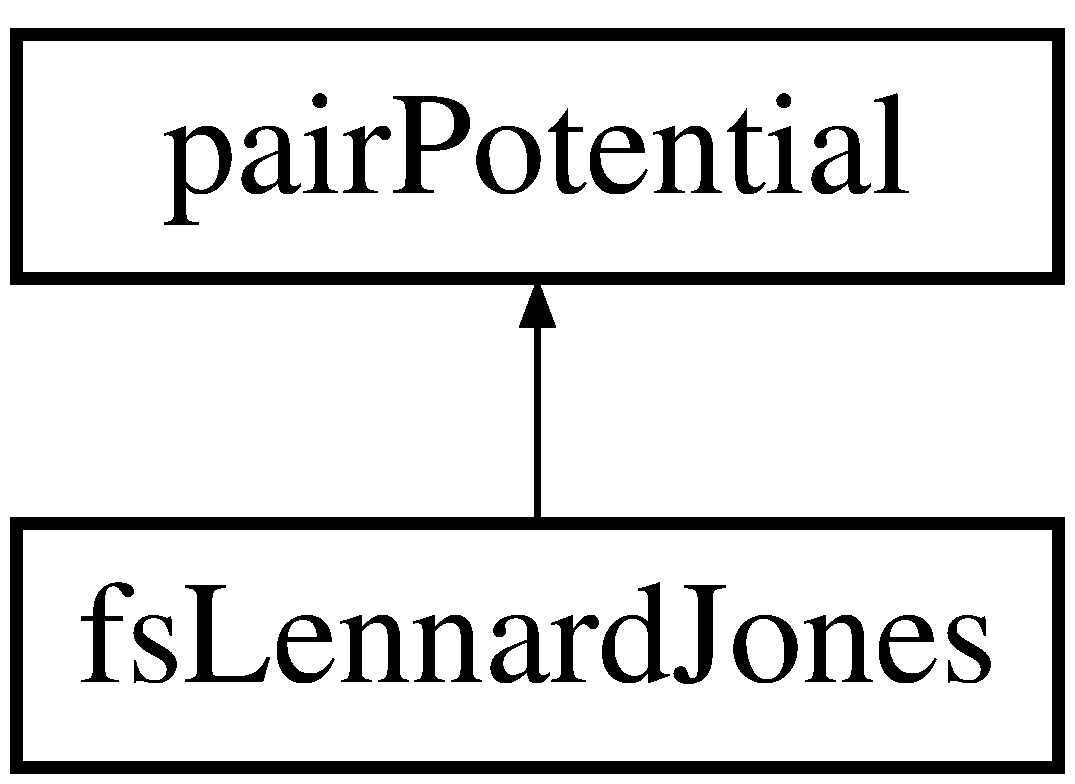
\includegraphics[height=2.000000cm]{classfs_lennard_jones}
\end{center}
\end{figure}
\subsection*{Public Member Functions}
\begin{DoxyCompactItemize}
\item 
\hyperlink{classfs_lennard_jones_a3ac9865901b9b36e4ef1dafdd2f059ad}{$\sim$fs\-Lennard\-Jones} ()
\item 
void \hyperlink{classfs_lennard_jones_a374bec4ba1510893ef2765251b978c47}{set\-Parameters} (const std\-::vector$<$ double $>$ params)
\begin{DoxyCompactList}\small\item\em Set the parameters in the Force-\/\-Shift Lennard-\/\-Jones equation. \end{DoxyCompactList}\item 
double \hyperlink{classfs_lennard_jones_a2f45293eeb451446a45349abd23342e1}{energy} (const \hyperlink{classatom}{atom} $\ast$a1, const \hyperlink{classatom}{atom} $\ast$a2, const std\-::vector$<$ double $>$ \&box)
\begin{DoxyCompactList}\small\item\em Return the energy of two particles. \end{DoxyCompactList}\item 
double \hyperlink{classfs_lennard_jones_a342461a06106980e3e476956b83950bc}{tail\-Correction} (const double rho\-Bath)
\begin{DoxyCompactList}\small\item\em Tail correction for Force-\/\-Shifted Lennard-\/\-Jones is, by definition, zero always. \end{DoxyCompactList}\item 
double \hyperlink{classfs_lennard_jones_aaee77a863f5e681c43fdc67fecf10345}{rcut} ()
\begin{DoxyCompactList}\small\item\em Return the value of r\-\_\-\{cut\} for this potential. \end{DoxyCompactList}\end{DoxyCompactItemize}
\subsection*{Additional Inherited Members}


\subsection{Detailed Description}
Force-\/\-Shifted Lennard-\/\-Jones Potential Parameters should be specified in the following order\-: \{ epsilon, sigma, r\-\_\-cut, Mtot \}. 

Definition at line 60 of file potentials.\-h.



\subsection{Constructor \& Destructor Documentation}
\hypertarget{classfs_lennard_jones_a3ac9865901b9b36e4ef1dafdd2f059ad}{\index{fs\-Lennard\-Jones@{fs\-Lennard\-Jones}!$\sim$fs\-Lennard\-Jones@{$\sim$fs\-Lennard\-Jones}}
\index{$\sim$fs\-Lennard\-Jones@{$\sim$fs\-Lennard\-Jones}!fsLennardJones@{fs\-Lennard\-Jones}}
\subsubsection[{$\sim$fs\-Lennard\-Jones}]{\setlength{\rightskip}{0pt plus 5cm}fs\-Lennard\-Jones\-::$\sim$fs\-Lennard\-Jones (
\begin{DoxyParamCaption}
{}
\end{DoxyParamCaption}
)\hspace{0.3cm}{\ttfamily [inline]}}}\label{classfs_lennard_jones_a3ac9865901b9b36e4ef1dafdd2f059ad}


Definition at line 62 of file potentials.\-h.


\begin{DoxyCode}
62 \{;\}
\end{DoxyCode}


\subsection{Member Function Documentation}
\hypertarget{classfs_lennard_jones_a2f45293eeb451446a45349abd23342e1}{\index{fs\-Lennard\-Jones@{fs\-Lennard\-Jones}!energy@{energy}}
\index{energy@{energy}!fsLennardJones@{fs\-Lennard\-Jones}}
\subsubsection[{energy}]{\setlength{\rightskip}{0pt plus 5cm}double fs\-Lennard\-Jones\-::energy (
\begin{DoxyParamCaption}
\item[{const {\bf atom} $\ast$}]{a1, }
\item[{const {\bf atom} $\ast$}]{a2, }
\item[{const std\-::vector$<$ double $>$ \&}]{box}
\end{DoxyParamCaption}
)\hspace{0.3cm}{\ttfamily [virtual]}}}\label{classfs_lennard_jones_a2f45293eeb451446a45349abd23342e1}


Return the energy of two particles. 

\[ U(r) = U_{LJ}(r) - \frac{\del U_{LJ}(r_{cut})}{\del r}(r - r_{cut}) - U_{LJ}(r_{cut}) \quad r < r_{cut} \]


\begin{DoxyParams}[1]{Parameters}
\mbox{\tt in}  & {\em a1} & Atom 1 \\
\hline
\mbox{\tt in}  & {\em a2} & Atom 2 \\
\hline
\mbox{\tt in}  & {\em box} & Simulation box dimensions\\
\hline
\end{DoxyParams}
\begin{DoxyReturn}{Returns}
U(r) 
\end{DoxyReturn}


Implements \hyperlink{classpair_potential_a2b1e50ef9b6e50b01d89d31d5460ad76}{pair\-Potential}.



Definition at line 101 of file potentials.\-cpp.



References atom\-::m\-State, pair\-Potential\-::params\-\_\-, pair\-Potential\-::params\-Are\-Set\-\_\-, pbc\-Dist2(), and atom\-::pos.


\begin{DoxyCode}
101                                                                                               \{
102     \textcolor{keywordflow}{if} (!\hyperlink{classpair_potential_a635755c0a952bfc05a4cfae230c3dbd2}{paramsAreSet\_}) \{
103         \textcolor{keywordflow}{throw} \hyperlink{classcustom_exception}{customException} (\textcolor{stringliteral}{"For fsLennardJones parameters not set"});
104     \}
105 
106     \textcolor{keyword}{const} \textcolor{keywordtype}{double} r\_sq = \hyperlink{utilities_8cpp_abb1db3a8a3ac46e044bbe7b2c5684c0a}{pbcDist2}(a1->\hyperlink{classatom_a3ae5f4880e7831d8b2c9fda72b4eb24a}{pos}, a2->\hyperlink{classatom_a3ae5f4880e7831d8b2c9fda72b4eb24a}{pos}, box);
107 
108     \textcolor{comment}{// only one of these atoms (at most) should be "partially" inserted}
109     \textcolor{keywordtype}{int} mState = 0;
110     \textcolor{keywordflow}{if} (a1->\hyperlink{classatom_a3cb00c0c5b7533657e05af6ff4a42740}{mState} != 0) \{
111         mState = a1->\hyperlink{classatom_a3cb00c0c5b7533657e05af6ff4a42740}{mState};
112     \}
113     \textcolor{keywordflow}{if} (a2->\hyperlink{classatom_a3cb00c0c5b7533657e05af6ff4a42740}{mState} != 0) \{
114         mState = a2->\hyperlink{classatom_a3cb00c0c5b7533657e05af6ff4a42740}{mState};
115     \}
116 
117     \textcolor{keyword}{const} \textcolor{keywordtype}{double} r2 = (sigmaM\_[mState]*sigmaM\_[mState]/r\_sq), r6 = r2*r2*r2, r12 = r6*r6;
118     \textcolor{keyword}{const} \textcolor{keywordtype}{double} r2c = (sigmaM\_[mState]*sigmaM\_[mState]/(\hyperlink{classpair_potential_abf8ec8af983d6e9960bd149da099e883}{params\_}[2]*
      \hyperlink{classpair_potential_abf8ec8af983d6e9960bd149da099e883}{params\_}[2])), r6c = r2c*r2c*r2c, r12c = r6c*r6c;
119     \textcolor{keywordflow}{if} (r\_sq < \hyperlink{classpair_potential_abf8ec8af983d6e9960bd149da099e883}{params\_}[2]*\hyperlink{classpair_potential_abf8ec8af983d6e9960bd149da099e883}{params\_}[2]) \{
120         \textcolor{keywordflow}{return} 4.0*epsM\_[mState]*(r12 - r6) - 4.0*epsM\_[mState]*(r12c - r6c) - (sqrt(r\_sq) - params\_[2])*(-
      24.0*epsM\_[mState]/params\_[2]*(2.0*r12c - r6c));
121     \} \textcolor{keywordflow}{else} \{
122         \textcolor{keywordflow}{return} 0.0;
123     \}
124 \}
\end{DoxyCode}
\hypertarget{classfs_lennard_jones_aaee77a863f5e681c43fdc67fecf10345}{\index{fs\-Lennard\-Jones@{fs\-Lennard\-Jones}!rcut@{rcut}}
\index{rcut@{rcut}!fsLennardJones@{fs\-Lennard\-Jones}}
\subsubsection[{rcut}]{\setlength{\rightskip}{0pt plus 5cm}double fs\-Lennard\-Jones\-::rcut (
\begin{DoxyParamCaption}
{}
\end{DoxyParamCaption}
)\hspace{0.3cm}{\ttfamily [virtual]}}}\label{classfs_lennard_jones_aaee77a863f5e681c43fdc67fecf10345}


Return the value of r\-\_\-\{cut\} for this potential. 

\begin{DoxyReturn}{Returns}
rcut 
\end{DoxyReturn}


Implements \hyperlink{classpair_potential_abf4f8d231c5e2e36d72916d33dcd75f0}{pair\-Potential}.



Definition at line 142 of file potentials.\-cpp.



References pair\-Potential\-::params\-\_\-, and pair\-Potential\-::params\-Are\-Set\-\_\-.


\begin{DoxyCode}
142                              \{
143     \textcolor{keywordflow}{if} (!\hyperlink{classpair_potential_a635755c0a952bfc05a4cfae230c3dbd2}{paramsAreSet\_}) \{
144         \textcolor{keywordflow}{throw} \hyperlink{classcustom_exception}{customException} (\textcolor{stringliteral}{"For fsLennardJones parameters not set"});
145     \} \textcolor{keywordflow}{else} \{
146         \textcolor{keywordflow}{return} \hyperlink{classpair_potential_abf8ec8af983d6e9960bd149da099e883}{params\_}[2];
147     \}
148 \}
\end{DoxyCode}
\hypertarget{classfs_lennard_jones_a374bec4ba1510893ef2765251b978c47}{\index{fs\-Lennard\-Jones@{fs\-Lennard\-Jones}!set\-Parameters@{set\-Parameters}}
\index{set\-Parameters@{set\-Parameters}!fsLennardJones@{fs\-Lennard\-Jones}}
\subsubsection[{set\-Parameters}]{\setlength{\rightskip}{0pt plus 5cm}void fs\-Lennard\-Jones\-::set\-Parameters (
\begin{DoxyParamCaption}
\item[{const std\-::vector$<$ double $>$}]{params}
\end{DoxyParamCaption}
)\hspace{0.3cm}{\ttfamily [virtual]}}}\label{classfs_lennard_jones_a374bec4ba1510893ef2765251b978c47}


Set the parameters in the Force-\/\-Shift Lennard-\/\-Jones equation. 


\begin{DoxyParams}[1]{Parameters}
\mbox{\tt in}  & {\em params} & Vector of inputs\-: \{epsilon, sigma, r\-\_\-cut, Mtot\} \\
\hline
\end{DoxyParams}


Implements \hyperlink{classpair_potential_ad4b237646f9de2ae9f95cc9350564bc5}{pair\-Potential}.



Definition at line 37 of file potentials.\-cpp.



References pair\-Potential\-::params\-\_\-, pair\-Potential\-::params\-Are\-Set\-\_\-, and pair\-Potential\-::use\-Tail\-Correction.


\begin{DoxyCode}
37                                                                      \{
38     \textcolor{keywordflow}{if} (params.size() != 4) \{
39         \textcolor{keywordflow}{throw} \hyperlink{classcustom_exception}{customException} (\textcolor{stringliteral}{"For fsLennardJones must specify 5 parameters: epsilon,
       sigma, r\_cut, Mtot"});
40     \} \textcolor{keywordflow}{else} \{
41         \textcolor{keywordflow}{if} (params[0] < 0) \{
42             \textcolor{keywordflow}{throw} \hyperlink{classcustom_exception}{customException} (\textcolor{stringliteral}{"For fsLennardJones, epsilon > 0"});
43         \}
44         \textcolor{keywordflow}{if} (params[1] < 0) \{
45             \textcolor{keywordflow}{throw} \hyperlink{classcustom_exception}{customException} (\textcolor{stringliteral}{"For fsLennardJones, sigma > 0"});
46         \}
47         \textcolor{keywordflow}{if} (params[2] < 0) \{
48             \textcolor{keywordflow}{throw} \hyperlink{classcustom_exception}{customException} (\textcolor{stringliteral}{"For fsLennardJones, r\_cut > 0"});
49         \}
50         \textcolor{keywordflow}{if} (\textcolor{keywordtype}{int}(params[3]) < 1) \{
51             \textcolor{keywordflow}{throw} \hyperlink{classcustom_exception}{customException} (\textcolor{stringliteral}{"For fsLennardJones, total expanded ensemble states, Mtot
       >= 1"});
52         \}
53 
54         \hyperlink{classpair_potential_a635755c0a952bfc05a4cfae230c3dbd2}{paramsAreSet\_} = \textcolor{keyword}{true};
55         \hyperlink{classpair_potential_abf8ec8af983d6e9960bd149da099e883}{params\_} = params;
56 
57         \hyperlink{classpair_potential_ab4b4538a7e13771f50a29aaac2443037}{useTailCorrection} = \textcolor{keyword}{false};
58 
59         \textcolor{comment}{// use a "constant volume" scheme to distribute the stages}
60         sigmaM\_.resize(\textcolor{keywordtype}{int}(params[3]), 0);
61         \textcolor{keywordflow}{for} (\textcolor{keywordtype}{int} i = 0; i < sigmaM\_.size(); ++i) \{
62             \textcolor{keywordflow}{if} (i == 0) \{
63                 \textcolor{comment}{// fully inserted}
64                 sigmaM\_[i] = params[1];
65             \} \textcolor{keywordflow}{else} \{
66                 \textcolor{comment}{// use volume scaling so each stage is separated from its neighbors by the same dV}
67                 \textcolor{keywordtype}{double} lastSigma = 0;
68                 \textcolor{keywordflow}{if} (i == 1) \{
69                     lastSigma = 0;
70                 \} \textcolor{keywordflow}{else} \{
71                     lastSigma = sigmaM\_[i-1];
72                 \}
73                 sigmaM\_[i] = pow(params[1]*params[1]*params[1]/(8.0*\textcolor{keywordtype}{int}(params[3])) + lastSigma*lastSigma*
      lastSigma, 1./3.);
74             \}
75         \}
76 
77         \textcolor{comment}{// scale energy linearly across the stages}
78         epsM\_.resize(\textcolor{keywordtype}{int}(params[3]), 0);
79         \textcolor{keywordflow}{for} (\textcolor{keywordtype}{int} i = 0; i < epsM\_.size(); ++i) \{
80             \textcolor{keywordflow}{if} (i == 0) \{
81                 \textcolor{comment}{// fully inserted}
82                 epsM\_[i] = params[0];
83             \} \textcolor{keywordflow}{else} \{
84                 epsM\_[i] = i*(params[0]/int(params[3]));
85             \}
86         \}
87     \}
88 \}
\end{DoxyCode}
\hypertarget{classfs_lennard_jones_a342461a06106980e3e476956b83950bc}{\index{fs\-Lennard\-Jones@{fs\-Lennard\-Jones}!tail\-Correction@{tail\-Correction}}
\index{tail\-Correction@{tail\-Correction}!fsLennardJones@{fs\-Lennard\-Jones}}
\subsubsection[{tail\-Correction}]{\setlength{\rightskip}{0pt plus 5cm}double fs\-Lennard\-Jones\-::tail\-Correction (
\begin{DoxyParamCaption}
\item[{const double}]{rho\-Bath}
\end{DoxyParamCaption}
)\hspace{0.3cm}{\ttfamily [virtual]}}}\label{classfs_lennard_jones_a342461a06106980e3e476956b83950bc}


Tail correction for Force-\/\-Shifted Lennard-\/\-Jones is, by definition, zero always. 


\begin{DoxyParams}[1]{Parameters}
\mbox{\tt in}  & {\em rho\-Bath} & Number density of the surrounding fluid\\
\hline
\end{DoxyParams}
\begin{DoxyReturn}{Returns}
U\-\_\-tail 
\end{DoxyReturn}


Implements \hyperlink{classpair_potential_a5387d21d8d487d1d42e9eaf7cae9175b}{pair\-Potential}.



Definition at line 133 of file potentials.\-cpp.


\begin{DoxyCode}
133                                                           \{
134     \textcolor{keywordflow}{return} 0.0;
135 \}
\end{DoxyCode}


The documentation for this class was generated from the following files\-:\begin{DoxyCompactItemize}
\item 
/home/nam4/\-Desktop/sandbox/\-F\-H\-M\-C\-Simulation/src/\hyperlink{potentials_8h}{potentials.\-h}\item 
/home/nam4/\-Desktop/sandbox/\-F\-H\-M\-C\-Simulation/src/\hyperlink{potentials_8cpp}{potentials.\-cpp}\end{DoxyCompactItemize}

\hypertarget{classhard_core}{\section{hard\-Core Class Reference}
\label{classhard_core}\index{hard\-Core@{hard\-Core}}
}


Hard-\/core potential Parameters should be specified in the following order\-: \{ sigma, Mtot \}.  




{\ttfamily \#include $<$potentials.\-h$>$}

Inheritance diagram for hard\-Core\-:\begin{figure}[H]
\begin{center}
\leavevmode
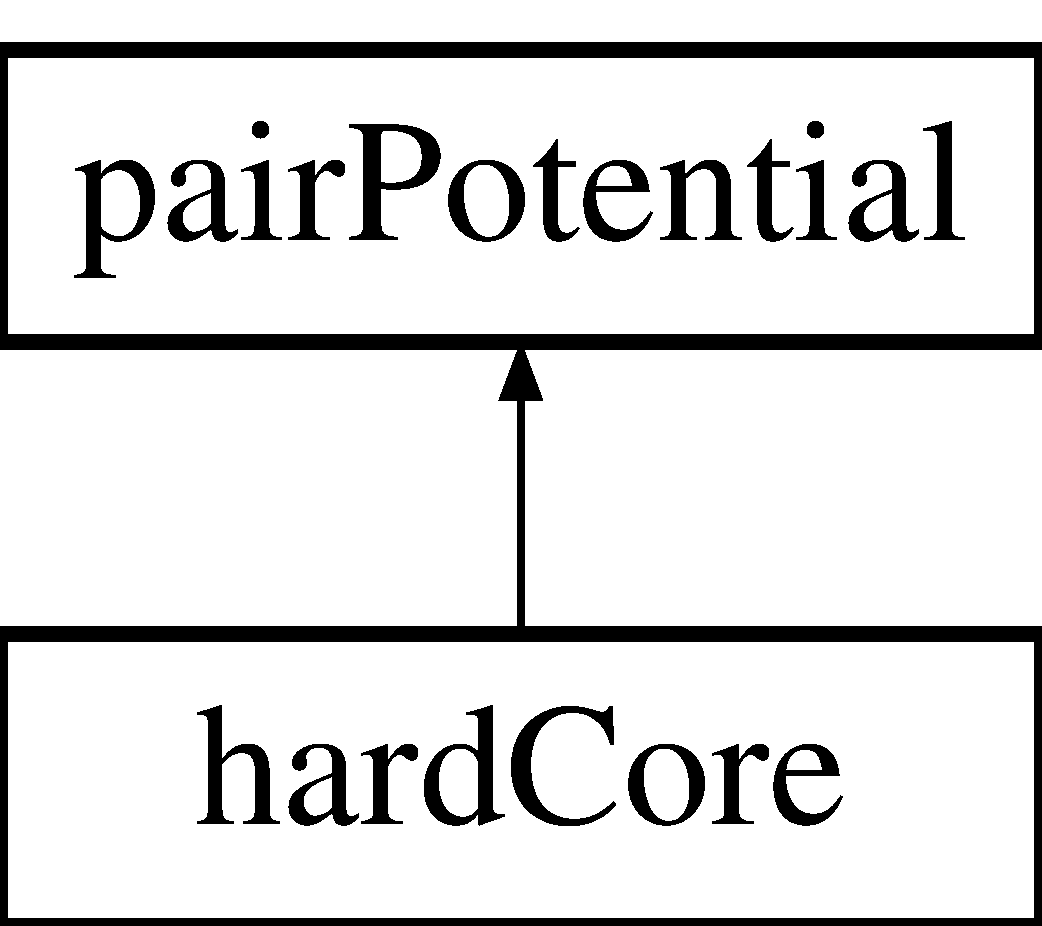
\includegraphics[height=2.000000cm]{classhard_core}
\end{center}
\end{figure}
\subsection*{Public Member Functions}
\begin{DoxyCompactItemize}
\item 
\hyperlink{classhard_core_aea5b04b2f9271269d6365ff7ed633151}{$\sim$hard\-Core} ()
\item 
void \hyperlink{classhard_core_a2bbf6a77445f5cb5fc1a3c37ba0e6566}{set\-Parameters} (const std\-::vector$<$ double $>$ params)
\begin{DoxyCompactList}\small\item\em Set the parameters in the hard-\/core potential. \end{DoxyCompactList}\item 
double \hyperlink{classhard_core_a8b7bb56ce5c3ad31a74d352da76164e2}{energy} (const \hyperlink{classatom}{atom} $\ast$a1, const \hyperlink{classatom}{atom} $\ast$a2, const std\-::vector$<$ double $>$ \&box)
\begin{DoxyCompactList}\small\item\em Return the energy of two particles. \end{DoxyCompactList}\item 
double \hyperlink{classhard_core_a90c73dbda39a9c48f1f26474474183e4}{tail\-Correction} (const double rho\-Bath)
\begin{DoxyCompactList}\small\item\em Tail correction for a hard core potential always returns 0 radius. \end{DoxyCompactList}\item 
double \hyperlink{classhard_core_a3cbf5ecde18b2f2798a4b1aba1801ca5}{rcut} ()
\begin{DoxyCompactList}\small\item\em Return the value of r\-\_\-\{cut\} for this potential. \end{DoxyCompactList}\end{DoxyCompactItemize}
\subsection*{Additional Inherited Members}


\subsection{Detailed Description}
Hard-\/core potential Parameters should be specified in the following order\-: \{ sigma, Mtot \}. 

Definition at line 114 of file potentials.\-h.



\subsection{Constructor \& Destructor Documentation}
\hypertarget{classhard_core_aea5b04b2f9271269d6365ff7ed633151}{\index{hard\-Core@{hard\-Core}!$\sim$hard\-Core@{$\sim$hard\-Core}}
\index{$\sim$hard\-Core@{$\sim$hard\-Core}!hardCore@{hard\-Core}}
\subsubsection[{$\sim$hard\-Core}]{\setlength{\rightskip}{0pt plus 5cm}hard\-Core\-::$\sim$hard\-Core (
\begin{DoxyParamCaption}
{}
\end{DoxyParamCaption}
)\hspace{0.3cm}{\ttfamily [inline]}}}\label{classhard_core_aea5b04b2f9271269d6365ff7ed633151}


Definition at line 116 of file potentials.\-h.


\begin{DoxyCode}
116 \{;\}
\end{DoxyCode}


\subsection{Member Function Documentation}
\hypertarget{classhard_core_a8b7bb56ce5c3ad31a74d352da76164e2}{\index{hard\-Core@{hard\-Core}!energy@{energy}}
\index{energy@{energy}!hardCore@{hard\-Core}}
\subsubsection[{energy}]{\setlength{\rightskip}{0pt plus 5cm}double hard\-Core\-::energy (
\begin{DoxyParamCaption}
\item[{const {\bf atom} $\ast$}]{a1, }
\item[{const {\bf atom} $\ast$}]{a2, }
\item[{const std\-::vector$<$ double $>$ \&}]{box}
\end{DoxyParamCaption}
)\hspace{0.3cm}{\ttfamily [virtual]}}}\label{classhard_core_a8b7bb56ce5c3ad31a74d352da76164e2}


Return the energy of two particles. 


\begin{DoxyParams}[1]{Parameters}
\mbox{\tt in}  & {\em a1} & Atom 1 \\
\hline
\mbox{\tt in}  & {\em a2} & Atom 2 \\
\hline
\mbox{\tt in}  & {\em box} & Simulation box dimensions\\
\hline
\end{DoxyParams}
\begin{DoxyReturn}{Returns}
U(r) 
\end{DoxyReturn}


Implements \hyperlink{classpair_potential_a2b1e50ef9b6e50b01d89d31d5460ad76}{pair\-Potential}.



Definition at line 609 of file potentials.\-cpp.



References atom\-::m\-State, N\-U\-M\-\_\-\-I\-N\-F\-I\-N\-I\-T\-Y, pair\-Potential\-::params\-Are\-Set\-\_\-, pbc\-Dist2(), and atom\-::pos.


\begin{DoxyCode}
609                                                                                         \{
610     \textcolor{keywordflow}{if} (!\hyperlink{classpair_potential_a635755c0a952bfc05a4cfae230c3dbd2}{paramsAreSet\_}) \{
611         \textcolor{keywordflow}{throw} \hyperlink{classcustom_exception}{customException} (\textcolor{stringliteral}{"For hardCore parameters not set"});
612     \}
613 
614     \textcolor{keywordtype}{int} mState = 0;
615     \textcolor{keywordflow}{if} (a1->\hyperlink{classatom_a3cb00c0c5b7533657e05af6ff4a42740}{mState} != 0) \{
616         mState = a1->\hyperlink{classatom_a3cb00c0c5b7533657e05af6ff4a42740}{mState};
617     \}
618     \textcolor{keywordflow}{if} (a2->\hyperlink{classatom_a3cb00c0c5b7533657e05af6ff4a42740}{mState} != 0) \{
619         mState = a2->\hyperlink{classatom_a3cb00c0c5b7533657e05af6ff4a42740}{mState};
620     \}
621 
622     \textcolor{keyword}{const} \textcolor{keywordtype}{double} r = sqrt(\hyperlink{utilities_8cpp_abb1db3a8a3ac46e044bbe7b2c5684c0a}{pbcDist2}(a1->\hyperlink{classatom_a3ae5f4880e7831d8b2c9fda72b4eb24a}{pos}, a2->\hyperlink{classatom_a3ae5f4880e7831d8b2c9fda72b4eb24a}{pos}, box));
623 
624     \textcolor{keywordflow}{if} (r < sigmaM\_[mState]) \{
625         \textcolor{keywordflow}{return} \hyperlink{potentials_8h_ab94ab1d09e2291d03fe92a0e24a9d33b}{NUM\_INFINITY};
626     \} \textcolor{keywordflow}{else} \{
627         \textcolor{keywordflow}{return} 0.0;
628     \}
629 \}
\end{DoxyCode}
\hypertarget{classhard_core_a3cbf5ecde18b2f2798a4b1aba1801ca5}{\index{hard\-Core@{hard\-Core}!rcut@{rcut}}
\index{rcut@{rcut}!hardCore@{hard\-Core}}
\subsubsection[{rcut}]{\setlength{\rightskip}{0pt plus 5cm}double hard\-Core\-::rcut (
\begin{DoxyParamCaption}
{}
\end{DoxyParamCaption}
)\hspace{0.3cm}{\ttfamily [virtual]}}}\label{classhard_core_a3cbf5ecde18b2f2798a4b1aba1801ca5}


Return the value of r\-\_\-\{cut\} for this potential. 

\begin{DoxyReturn}{Returns}
r\-\_\-cut 
\end{DoxyReturn}


Implements \hyperlink{classpair_potential_abf4f8d231c5e2e36d72916d33dcd75f0}{pair\-Potential}.



Definition at line 647 of file potentials.\-cpp.



References pair\-Potential\-::params\-\_\-, and pair\-Potential\-::params\-Are\-Set\-\_\-.


\begin{DoxyCode}
647                        \{
648     \textcolor{keywordflow}{if} (!\hyperlink{classpair_potential_a635755c0a952bfc05a4cfae230c3dbd2}{paramsAreSet\_}) \{
649         \textcolor{keywordflow}{throw} \hyperlink{classcustom_exception}{customException} (\textcolor{stringliteral}{"For hardCore parameters not set"});
650     \} \textcolor{keywordflow}{else} \{
651         \textcolor{keywordflow}{if} (fabs(\hyperlink{classpair_potential_abf8ec8af983d6e9960bd149da099e883}{params\_}[0]) < 1.0e-12) \{
652             \textcolor{comment}{// in case sigma = 0 (used for ideal gas case) just return finite value for cell lists}
653             \textcolor{keywordflow}{return} 1.0;
654         \} \textcolor{keywordflow}{else} \{
655             \textcolor{keywordflow}{return} (\hyperlink{classpair_potential_abf8ec8af983d6e9960bd149da099e883}{params\_}[0]);
656         \}
657     \}
658 \}
\end{DoxyCode}
\hypertarget{classhard_core_a2bbf6a77445f5cb5fc1a3c37ba0e6566}{\index{hard\-Core@{hard\-Core}!set\-Parameters@{set\-Parameters}}
\index{set\-Parameters@{set\-Parameters}!hardCore@{hard\-Core}}
\subsubsection[{set\-Parameters}]{\setlength{\rightskip}{0pt plus 5cm}void hard\-Core\-::set\-Parameters (
\begin{DoxyParamCaption}
\item[{const std\-::vector$<$ double $>$}]{params}
\end{DoxyParamCaption}
)\hspace{0.3cm}{\ttfamily [virtual]}}}\label{classhard_core_a2bbf6a77445f5cb5fc1a3c37ba0e6566}


Set the parameters in the hard-\/core potential. 


\begin{DoxyParams}[1]{Parameters}
\mbox{\tt in}  & {\em params} & Vector of inputs\-: \{sigma, Mtot\} \\
\hline
\end{DoxyParams}


Implements \hyperlink{classpair_potential_ad4b237646f9de2ae9f95cc9350564bc5}{pair\-Potential}.



Definition at line 564 of file potentials.\-cpp.



References pair\-Potential\-::params\-\_\-, pair\-Potential\-::params\-Are\-Set\-\_\-, and pair\-Potential\-::use\-Tail\-Correction.


\begin{DoxyCode}
564                                                                \{
565     \textcolor{keywordflow}{if} (params.size() != 2) \{
566         \textcolor{keywordflow}{throw} \hyperlink{classcustom_exception}{customException} (\textcolor{stringliteral}{"For hardCore must specify 2 parameter: sigma, Mtot"});
567     \} \textcolor{keywordflow}{else} \{
568         \textcolor{keywordflow}{if} (params[0] < 0) \{
569             \textcolor{keywordflow}{throw} \hyperlink{classcustom_exception}{customException} (\textcolor{stringliteral}{"For hardCore, sigma >= 0"});
570         \}
571         \textcolor{keywordflow}{if} (\textcolor{keywordtype}{int}(params[1]) < 1) \{
572             \textcolor{keywordflow}{throw} \hyperlink{classcustom_exception}{customException} (\textcolor{stringliteral}{"For hardCore, total expanded ensemble state, Mtot >= 1"})
      ;
573         \}
574 
575         \hyperlink{classpair_potential_abf8ec8af983d6e9960bd149da099e883}{params\_} = params;
576         \hyperlink{classpair_potential_a635755c0a952bfc05a4cfae230c3dbd2}{paramsAreSet\_} = \textcolor{keyword}{true};
577 
578         \hyperlink{classpair_potential_ab4b4538a7e13771f50a29aaac2443037}{useTailCorrection} = \textcolor{keyword}{false};
579 
580         \textcolor{comment}{// use a "constant volume" scheme to distribute the stages}
581         sigmaM\_.resize(\textcolor{keywordtype}{int}(params[1]), 0);
582         \textcolor{keywordflow}{for} (\textcolor{keywordtype}{int} i = 0; i < sigmaM\_.size(); ++i) \{
583             \textcolor{keywordflow}{if} (i == 0) \{
584                 \textcolor{comment}{// fully inserted}
585                 sigmaM\_[i] = params[0];
586             \} \textcolor{keywordflow}{else} \{
587                 \textcolor{comment}{// use volume scaling so each stage is separated from its neighbors by the same dV}
588                 \textcolor{keywordtype}{double} lastSigma = 0;
589                 \textcolor{keywordflow}{if} (i == 1) \{
590                     lastSigma = 0;
591                 \} \textcolor{keywordflow}{else} \{
592                     lastSigma = sigmaM\_[i-1];
593                 \}
594                 sigmaM\_[i] = pow(params[0]*params[0]*params[0]/(8.0*\textcolor{keywordtype}{int}(params[1])) + lastSigma*lastSigma*
      lastSigma, 1./3.);
595             \}
596         \}
597     \}
598 \}
\end{DoxyCode}
\hypertarget{classhard_core_a90c73dbda39a9c48f1f26474474183e4}{\index{hard\-Core@{hard\-Core}!tail\-Correction@{tail\-Correction}}
\index{tail\-Correction@{tail\-Correction}!hardCore@{hard\-Core}}
\subsubsection[{tail\-Correction}]{\setlength{\rightskip}{0pt plus 5cm}double hard\-Core\-::tail\-Correction (
\begin{DoxyParamCaption}
\item[{const double}]{rho\-Bath}
\end{DoxyParamCaption}
)\hspace{0.3cm}{\ttfamily [virtual]}}}\label{classhard_core_a90c73dbda39a9c48f1f26474474183e4}


Tail correction for a hard core potential always returns 0 radius. 


\begin{DoxyParams}[1]{Parameters}
\mbox{\tt in}  & {\em Number} & density of the surrounding fluid\\
\hline
\end{DoxyParams}
\begin{DoxyReturn}{Returns}
U\-\_\-tail 
\end{DoxyReturn}


Implements \hyperlink{classpair_potential_a5387d21d8d487d1d42e9eaf7cae9175b}{pair\-Potential}.



Definition at line 638 of file potentials.\-cpp.


\begin{DoxyCode}
638                                                     \{
639     \textcolor{keywordflow}{return} 0.0;
640 \}
\end{DoxyCode}


The documentation for this class was generated from the following files\-:\begin{DoxyCompactItemize}
\item 
/home/nam4/\-Desktop/sandbox/\-F\-H\-M\-C\-Simulation/src/\hyperlink{potentials_8h}{potentials.\-h}\item 
/home/nam4/\-Desktop/sandbox/\-F\-H\-M\-C\-Simulation/src/\hyperlink{potentials_8cpp}{potentials.\-cpp}\end{DoxyCompactItemize}

\hypertarget{classhard_wall_z}{\section{hard\-Wall\-Z Class Reference}
\label{classhard_wall_z}\index{hard\-Wall\-Z@{hard\-Wall\-Z}}
}


Parallel hard walls in the z-\/direction.  




{\ttfamily \#include $<$barrier.\-h$>$}

Inheritance diagram for hard\-Wall\-Z\-:\begin{figure}[H]
\begin{center}
\leavevmode
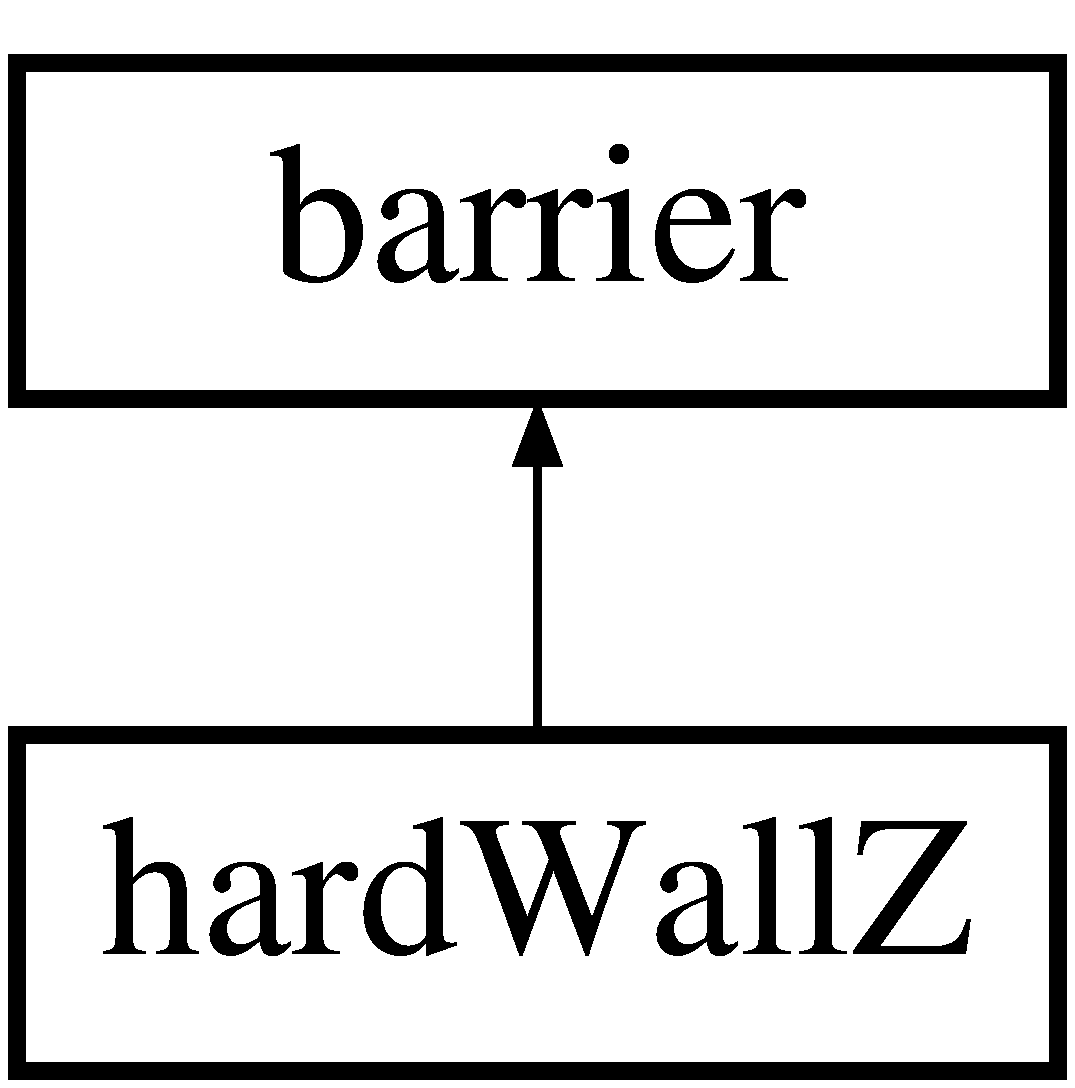
\includegraphics[height=2.000000cm]{classhard_wall_z}
\end{center}
\end{figure}
\subsection*{Public Member Functions}
\begin{DoxyCompactItemize}
\item 
\hyperlink{classhard_wall_z_a65910c4aca42a07e7ca0a12dbe25b895}{$\sim$hard\-Wall\-Z} ()
\item 
\hyperlink{classhard_wall_z_a0c04f7e529316bb89187a74ff3316f48}{hard\-Wall\-Z} (const double lb, const double ub, const double sigma, const int M=1)
\begin{DoxyCompactList}\small\item\em Instantiate a hard wall with boundaries in the +/-\/ z direction. \end{DoxyCompactList}\item 
bool \hyperlink{classhard_wall_z_ac4c72aa32e0cdfe40c6765642ffb78d7}{inside} (const \hyperlink{classatom}{atom} $\ast$a1, const std\-::vector$<$ double $>$ \&box)
\begin{DoxyCompactList}\small\item\em Return whether or not a point falls between the walls (subject to a hard-\/sphere exclusion radius). \end{DoxyCompactList}\item 
double \hyperlink{classhard_wall_z_ae1c05d46be694e7b071969f9511e4142}{energy} (const \hyperlink{classatom}{atom} $\ast$a1, const std\-::vector$<$ double $>$ \&box)
\begin{DoxyCompactList}\small\item\em Interaction energy with the wall. \end{DoxyCompactList}\end{DoxyCompactItemize}
\subsection*{Additional Inherited Members}


\subsection{Detailed Description}
Parallel hard walls in the z-\/direction. 

Definition at line 30 of file barrier.\-h.



\subsection{Constructor \& Destructor Documentation}
\hypertarget{classhard_wall_z_a65910c4aca42a07e7ca0a12dbe25b895}{\index{hard\-Wall\-Z@{hard\-Wall\-Z}!$\sim$hard\-Wall\-Z@{$\sim$hard\-Wall\-Z}}
\index{$\sim$hard\-Wall\-Z@{$\sim$hard\-Wall\-Z}!hardWallZ@{hard\-Wall\-Z}}
\subsubsection[{$\sim$hard\-Wall\-Z}]{\setlength{\rightskip}{0pt plus 5cm}hard\-Wall\-Z\-::$\sim$hard\-Wall\-Z (
\begin{DoxyParamCaption}
{}
\end{DoxyParamCaption}
)\hspace{0.3cm}{\ttfamily [inline]}}}\label{classhard_wall_z_a65910c4aca42a07e7ca0a12dbe25b895}


Definition at line 32 of file barrier.\-h.


\begin{DoxyCode}
32 \{\};
\end{DoxyCode}
\hypertarget{classhard_wall_z_a0c04f7e529316bb89187a74ff3316f48}{\index{hard\-Wall\-Z@{hard\-Wall\-Z}!hard\-Wall\-Z@{hard\-Wall\-Z}}
\index{hard\-Wall\-Z@{hard\-Wall\-Z}!hardWallZ@{hard\-Wall\-Z}}
\subsubsection[{hard\-Wall\-Z}]{\setlength{\rightskip}{0pt plus 5cm}hard\-Wall\-Z\-::hard\-Wall\-Z (
\begin{DoxyParamCaption}
\item[{const double}]{lb, }
\item[{const double}]{ub, }
\item[{const double}]{sigma, }
\item[{const int}]{M = {\ttfamily 1}}
\end{DoxyParamCaption}
)}}\label{classhard_wall_z_a0c04f7e529316bb89187a74ff3316f48}


Instantiate a hard wall with boundaries in the +/-\/ z direction. 

Expanded ensembles scale the range of interaction via the sigma parameter.


\begin{DoxyParams}[1]{Parameters}
\mbox{\tt in}  & {\em lb} & z-\/\-Position of the lower wall \\
\hline
\mbox{\tt in}  & {\em ub} & z-\/\-Position of the upper wall \\
\hline
\mbox{\tt in}  & {\em sigma} & Hard-\/sphere diameter the species this wall interacts with can approach within \\
\hline
\mbox{\tt in}  & {\em M} & Total number of expanded ensemble states possible for this atom type (defaults to 1) \\
\hline
\end{DoxyParams}


Definition at line 385 of file barrier.\-cpp.



References barrier\-::\-M\-\_\-.


\begin{DoxyCode}
385                                                                                        \{
386     \textcolor{keywordflow}{if} (lb >= ub) \{
387         \textcolor{keywordflow}{throw} \hyperlink{classcustom_exception}{customException} (\textcolor{stringliteral}{"hardWallZ must have lower bound < upper bound"});
388     \}
389     \textcolor{keywordflow}{if} (sigma < 0) \{
390         \textcolor{keywordflow}{throw} \hyperlink{classcustom_exception}{customException} (\textcolor{stringliteral}{"hardWallZ must have sigma >= 0"});
391     \}
392     \textcolor{keywordflow}{if} (M < 1) \{
393         \textcolor{keywordflow}{throw} \hyperlink{classcustom_exception}{customException} (\textcolor{stringliteral}{"hardWallZ must have M >= 1"});
394     \}
395 
396     sigma\_ = sigma;
397     ub\_ = ub;
398     lb\_ = lb;
399     \hyperlink{classbarrier_a274cf283ffc97c22ffa9a4258369c400}{M\_} = M;
400 \}
\end{DoxyCode}


\subsection{Member Function Documentation}
\hypertarget{classhard_wall_z_ae1c05d46be694e7b071969f9511e4142}{\index{hard\-Wall\-Z@{hard\-Wall\-Z}!energy@{energy}}
\index{energy@{energy}!hardWallZ@{hard\-Wall\-Z}}
\subsubsection[{energy}]{\setlength{\rightskip}{0pt plus 5cm}double hard\-Wall\-Z\-::energy (
\begin{DoxyParamCaption}
\item[{const {\bf atom} $\ast$}]{a1, }
\item[{const std\-::vector$<$ double $>$ \&}]{box}
\end{DoxyParamCaption}
)\hspace{0.3cm}{\ttfamily [virtual]}}}\label{classhard_wall_z_ae1c05d46be694e7b071969f9511e4142}


Interaction energy with the wall. 

Sigma is scaled linearly with expanded ensemble state.


\begin{DoxyParams}[1]{Parameters}
\mbox{\tt in}  & {\em a1} & Pointer to atom with position to test -\/ this does N\-O\-T need to be in the simulation box a priori \\
\hline
\mbox{\tt in}  & {\em box} & Simulation box \\
\hline
\end{DoxyParams}


Implements \hyperlink{classbarrier_a2d308cfd5709aa479d0b37733f1a0db7}{barrier}.



Definition at line 433 of file barrier.\-cpp.



References barrier\-::\-M\-\_\-, atom\-::m\-State, N\-U\-M\-\_\-\-I\-N\-F\-I\-N\-I\-T\-Y, pbc(), and atom\-::pos.


\begin{DoxyCode}
433                                                                          \{
434     std::vector < double > p = a1->\hyperlink{classatom_a3ae5f4880e7831d8b2c9fda72b4eb24a}{pos};
435     \hyperlink{utilities_8cpp_ad858a38f435e9a0ee890aa0f526714d2}{pbc} (p, box);
436 
437     \textcolor{keywordtype}{double} sig = sigma\_;
438     \textcolor{keywordflow}{if} (a1->\hyperlink{classatom_a3cb00c0c5b7533657e05af6ff4a42740}{mState} > 0) \{
439         sig = (sigma\_/\hyperlink{classbarrier_a274cf283ffc97c22ffa9a4258369c400}{M\_})*a1->\hyperlink{classatom_a3cb00c0c5b7533657e05af6ff4a42740}{mState};
440     \}
441     \textcolor{keywordflow}{if} (a1->\hyperlink{classatom_a3cb00c0c5b7533657e05af6ff4a42740}{mState} < 0 || a1->\hyperlink{classatom_a3cb00c0c5b7533657e05af6ff4a42740}{mState} > \hyperlink{classbarrier_a274cf283ffc97c22ffa9a4258369c400}{M\_}-1) \{
442         \textcolor{keywordflow}{throw} \hyperlink{classcustom_exception}{customException} (\textcolor{stringliteral}{"mState out of bounds for hardWallZ"});
443     \}
444 
445     \textcolor{keywordflow}{if} (p[2] >= ub\_ - sig/2.0 || p[2] <= lb\_ + sig/2.0) \{
446         \textcolor{keywordflow}{return} \hyperlink{potentials_8h_ab94ab1d09e2291d03fe92a0e24a9d33b}{NUM\_INFINITY};
447     \} \textcolor{keywordflow}{else} \{
448         \textcolor{keywordflow}{return} 0.0;
449     \}
450 \}
\end{DoxyCode}
\hypertarget{classhard_wall_z_ac4c72aa32e0cdfe40c6765642ffb78d7}{\index{hard\-Wall\-Z@{hard\-Wall\-Z}!inside@{inside}}
\index{inside@{inside}!hardWallZ@{hard\-Wall\-Z}}
\subsubsection[{inside}]{\setlength{\rightskip}{0pt plus 5cm}bool hard\-Wall\-Z\-::inside (
\begin{DoxyParamCaption}
\item[{const {\bf atom} $\ast$}]{a1, }
\item[{const std\-::vector$<$ double $>$ \&}]{box}
\end{DoxyParamCaption}
)\hspace{0.3cm}{\ttfamily [virtual]}}}\label{classhard_wall_z_ac4c72aa32e0cdfe40c6765642ffb78d7}


Return whether or not a point falls between the walls (subject to a hard-\/sphere exclusion radius). 

Sigma is scaled linearly with expanded ensemble state.


\begin{DoxyParams}[1]{Parameters}
\mbox{\tt in}  & {\em a1} & Pointer to atom with position to test -\/ this does N\-O\-T need to be in the simulation box a priori \\
\hline
\mbox{\tt in}  & {\em box} & Simulation box \\
\hline
\end{DoxyParams}


Implements \hyperlink{classbarrier_a948ebdcfac501cb75d1a1f045a7d9125}{barrier}.



Definition at line 408 of file barrier.\-cpp.



References barrier\-::\-M\-\_\-, atom\-::m\-State, pbc(), and atom\-::pos.


\begin{DoxyCode}
408                                                                        \{
409     std::vector < double > p = a1->\hyperlink{classatom_a3ae5f4880e7831d8b2c9fda72b4eb24a}{pos};
410     \hyperlink{utilities_8cpp_ad858a38f435e9a0ee890aa0f526714d2}{pbc} (p, box);
411 
412     \textcolor{keywordtype}{double} sig = sigma\_;
413     \textcolor{keywordflow}{if} (a1->\hyperlink{classatom_a3cb00c0c5b7533657e05af6ff4a42740}{mState} > 0) \{
414         sig = (sigma\_/\hyperlink{classbarrier_a274cf283ffc97c22ffa9a4258369c400}{M\_})*a1->\hyperlink{classatom_a3cb00c0c5b7533657e05af6ff4a42740}{mState};
415     \}
416     \textcolor{keywordflow}{if} (a1->\hyperlink{classatom_a3cb00c0c5b7533657e05af6ff4a42740}{mState} < 0 || a1->\hyperlink{classatom_a3cb00c0c5b7533657e05af6ff4a42740}{mState} > \hyperlink{classbarrier_a274cf283ffc97c22ffa9a4258369c400}{M\_}-1) \{
417         \textcolor{keywordflow}{throw} \hyperlink{classcustom_exception}{customException} (\textcolor{stringliteral}{"mState out of bounds for hardWallZ"});
418     \}
419 
420     \textcolor{keywordflow}{if} (p[2] >= ub\_ - sig/2.0 || p[2] <= lb\_ + sig/2.0) \{
421         \textcolor{keywordflow}{return} \textcolor{keyword}{false};
422     \} \textcolor{keywordflow}{else} \{
423         \textcolor{keywordflow}{return} \textcolor{keyword}{true};
424     \}
425 \}
\end{DoxyCode}


The documentation for this class was generated from the following files\-:\begin{DoxyCompactItemize}
\item 
/home/nam4/\-Desktop/sandbox/\-F\-H\-M\-C\-Simulation/src/\hyperlink{barrier_8h}{barrier.\-h}\item 
/home/nam4/\-Desktop/sandbox/\-F\-H\-M\-C\-Simulation/src/\hyperlink{barrier_8cpp}{barrier.\-cpp}\end{DoxyCompactItemize}

\hypertarget{classhistogram}{\section{histogram Class Reference}
\label{classhistogram}\index{histogram@{histogram}}
}


{\ttfamily \#include $<$histogram.\-h$>$}

\subsection*{Public Member Functions}
\begin{DoxyCompactItemize}
\item 
\hyperlink{classhistogram_a68bd76ab77437beeb77342469fb77a67}{$\sim$histogram} ()
\item 
\hyperlink{classhistogram_acc41cd1e3ace837a977caeeb00f6606e}{histogram} ()
\item 
\hyperlink{classhistogram_a5a9a8918737bbb82ad73e31ac2d98a8b}{histogram} (const std\-::vector$<$ double $>$ lbound, const std\-::vector$<$ double $>$ ubound, const std\-::vector$<$ long long unsigned int $>$ nbins)
\begin{DoxyCompactList}\small\item\em Instantiate a multidimensional histogram. \end{DoxyCompactList}\item 
void \hyperlink{classhistogram_a801d984fe018521444ee0bd0776ba8dc}{print} (const std\-::string file\-Name)
\begin{DoxyCompactList}\small\item\em Print R\-A\-W (U\-N-\/\-N\-O\-R\-M\-A\-L\-I\-Z\-E\-D) histogram to file. \end{DoxyCompactList}\item 
void \hyperlink{classhistogram_a665e7f6c052d4b306c6fe7d0c600f1c8}{increment} (const long long unsigned int address, const double val)
\begin{DoxyCompactList}\small\item\em Increment the histogram by a given value at a given address. \end{DoxyCompactList}\item 
void \hyperlink{classhistogram_a1deef1080cd972343d7d5d8e5ef3a9f5}{increment} (const std\-::vector$<$ double $>$ \&coords, const double val)
\begin{DoxyCompactList}\small\item\em Increment the histogram by a given value at a given coordinate. \end{DoxyCompactList}\item 
void \hyperlink{classhistogram_aab27615593d020ca4de29c586c92af37}{set} (const std\-::vector$<$ double $>$ \&h, const std\-::vector$<$ double $>$ \&ctr)
\begin{DoxyCompactList}\small\item\em Assign the histogram and its corresponding counter. \end{DoxyCompactList}\item 
const long long unsigned int \hyperlink{classhistogram_ae52fa58934b56e05846a66e43c3184bd}{get\-Address} (const std\-::vector$<$ double $>$ \&coords)
\begin{DoxyCompactList}\small\item\em Get the linear address of the multidimensional coordinate. \end{DoxyCompactList}\item 
const std\-::vector$<$ double $>$ \hyperlink{classhistogram_a51aaf60b509809204f21934a18005b38}{get\-Coords} (long long unsigned int address)
\begin{DoxyCompactList}\small\item\em Given an address, return the (center of the) coordinate this refers to. \end{DoxyCompactList}\item 
std\-::vector$<$ double $>$ \hyperlink{classhistogram_afa81289dc32207eb3c44f8bd746f0d1d}{get\-Raw\-Histogram} ()
\begin{DoxyCompactList}\small\item\em Return the current histogram. \end{DoxyCompactList}\item 
std\-::vector$<$ double $>$ \hyperlink{classhistogram_a7d3541bd86551053f9fda7b5ae81e3e8}{get\-Counter} ()
\begin{DoxyCompactList}\small\item\em Return the current histogram counter. \end{DoxyCompactList}\end{DoxyCompactItemize}


\subsection{Detailed Description}


Definition at line 13 of file histogram.\-h.



\subsection{Constructor \& Destructor Documentation}
\hypertarget{classhistogram_a68bd76ab77437beeb77342469fb77a67}{\index{histogram@{histogram}!$\sim$histogram@{$\sim$histogram}}
\index{$\sim$histogram@{$\sim$histogram}!histogram@{histogram}}
\subsubsection[{$\sim$histogram}]{\setlength{\rightskip}{0pt plus 5cm}histogram\-::$\sim$histogram (
\begin{DoxyParamCaption}
{}
\end{DoxyParamCaption}
)\hspace{0.3cm}{\ttfamily [inline]}}}\label{classhistogram_a68bd76ab77437beeb77342469fb77a67}


Definition at line 15 of file histogram.\-h.


\begin{DoxyCode}
15 \{;\}
\end{DoxyCode}
\hypertarget{classhistogram_acc41cd1e3ace837a977caeeb00f6606e}{\index{histogram@{histogram}!histogram@{histogram}}
\index{histogram@{histogram}!histogram@{histogram}}
\subsubsection[{histogram}]{\setlength{\rightskip}{0pt plus 5cm}histogram\-::histogram (
\begin{DoxyParamCaption}
{}
\end{DoxyParamCaption}
)\hspace{0.3cm}{\ttfamily [inline]}}}\label{classhistogram_acc41cd1e3ace837a977caeeb00f6606e}


Definition at line 16 of file histogram.\-h.


\begin{DoxyCode}
16 \{;\}
\end{DoxyCode}
\hypertarget{classhistogram_a5a9a8918737bbb82ad73e31ac2d98a8b}{\index{histogram@{histogram}!histogram@{histogram}}
\index{histogram@{histogram}!histogram@{histogram}}
\subsubsection[{histogram}]{\setlength{\rightskip}{0pt plus 5cm}histogram\-::histogram (
\begin{DoxyParamCaption}
\item[{const std\-::vector$<$ double $>$}]{lbound, }
\item[{const std\-::vector$<$ double $>$}]{ubound, }
\item[{const std\-::vector$<$ long long unsigned int $>$}]{nbins}
\end{DoxyParamCaption}
)}}\label{classhistogram_a5a9a8918737bbb82ad73e31ac2d98a8b}


Instantiate a multidimensional histogram. 

Bounds and widths must be specified for each dimension. A bin is considered \char`\"{}centered\char`\"{} on its value.


\begin{DoxyParams}[1]{Parameters}
\mbox{\tt in}  & {\em lbound} & Vector of lower bounds for each dimension \\
\hline
\mbox{\tt in}  & {\em ubound} & Vector of upper bounds for each dimension \\
\hline
\mbox{\tt in}  & {\em nbins} & Number of bins to use along each dimension \\
\hline
\end{DoxyParams}


Definition at line 178 of file histogram.\-cpp.


\begin{DoxyCode}
178                                                                                                            
                                 \{
179     \textcolor{keywordflow}{if} (lbound.size() != ubound.size()) \{
180         \textcolor{keywordflow}{throw} \hyperlink{classcustom_exception}{customException} (\textcolor{stringliteral}{"Upper and lower bounds for histogram do have the same size"})
      ;
181     \}
182     \textcolor{keywordflow}{if} (nbins.size() != lbound.size()) \{
183         \textcolor{keywordflow}{throw} \hyperlink{classcustom_exception}{customException} (\textcolor{stringliteral}{"Number of bins for histogram's dimensions does not have the
       same size as its bounds"});
184     \}
185 
186     dim\_ = nbins.size();
187     widths\_.resize(dim\_, 0);
188     delta\_.resize(dim\_, 0);
189 
190     size\_ = 1;
191     \textcolor{keywordflow}{for} (\textcolor{keywordtype}{unsigned} \textcolor{keywordtype}{int} i = 0; i < dim\_; ++i) \{
192         \textcolor{keywordflow}{if} (lbound[i] > ubound[i]) \{
193             \textcolor{keywordflow}{throw} \hyperlink{classcustom_exception}{customException} (\textcolor{stringliteral}{"Lower bound > upper bound illegal for a histogram"});
194         \}
195 
196         \textcolor{keywordflow}{if} (lbound[i] < ubound[i]) \{
197             \textcolor{keywordflow}{if} (nbins[i] <= 1) \{
198                 \textcolor{keywordflow}{throw} \hyperlink{classcustom_exception}{customException} (\textcolor{stringliteral}{"Must > 1 bins for each dimensions in the histogram"})
      ;
199             \}
200             size\_ *= nbins[i];
201             delta\_[i] = (ubound[i] - lbound[i])/(nbins[i]-1);
202         \} \textcolor{keywordflow}{else} \{
203             \textcolor{comment}{// special case when upper and lower bound are the same (nbins = 1)}
204             \textcolor{keywordflow}{if} (nbins[i] != 1) \{
205                 \textcolor{keywordflow}{throw} \hyperlink{classcustom_exception}{customException} (\textcolor{stringliteral}{"nbins must be 1 if upper and lower bounds are equal
       in histogram"});
206             \}
207             size\_ *= nbins[i];
208             delta\_[i] = 1.0; \textcolor{comment}{// arbitrary}
209         \}
210 
211         \textcolor{comment}{// build projected widths}
212         \textcolor{keywordflow}{if} (i == 0) \{
213             widths\_[i] = 1;
214         \} \textcolor{keywordflow}{else} \{
215             widths\_[i] = widths\_[i-1]*nbins[i-1];
216         \}
217     \}
218 
219     lbound\_ = lbound;
220     ubound\_ = ubound;
221     nbins\_ = nbins;
222 
223     \textcolor{comment}{// initialize the histogram to 0}
224     \textcolor{keywordflow}{try} \{
225         h\_.resize(size\_, 0);
226     \} \textcolor{keywordflow}{catch} (std::bad\_alloc &ba) \{
227         \textcolor{keywordflow}{throw} \hyperlink{classcustom_exception}{customException} (\textcolor{stringliteral}{"Out of memory for histogram"});
228     \}
229     \textcolor{keywordflow}{try} \{
230         counter\_.resize(size\_, 0);
231     \} \textcolor{keywordflow}{catch} (std::bad\_alloc &ba) \{
232         \textcolor{keywordflow}{throw} \hyperlink{classcustom_exception}{customException} (\textcolor{stringliteral}{"Out of memory for histogram"});
233     \}
234 \}
\end{DoxyCode}


\subsection{Member Function Documentation}
\hypertarget{classhistogram_ae52fa58934b56e05846a66e43c3184bd}{\index{histogram@{histogram}!get\-Address@{get\-Address}}
\index{get\-Address@{get\-Address}!histogram@{histogram}}
\subsubsection[{get\-Address}]{\setlength{\rightskip}{0pt plus 5cm}const long long unsigned int histogram\-::get\-Address (
\begin{DoxyParamCaption}
\item[{const std\-::vector$<$ double $>$ \&}]{coords}
\end{DoxyParamCaption}
)}}\label{classhistogram_ae52fa58934b56e05846a66e43c3184bd}


Get the linear address of the multidimensional coordinate. 


\begin{DoxyParams}[1]{Parameters}
\mbox{\tt in}  & {\em coords} & Coordinates \\
\hline
\end{DoxyParams}


Definition at line 273 of file histogram.\-cpp.



Referenced by increment(), sim\-System\-::print\-Ext\-Moments(), and sim\-System\-::restart\-Ext\-Moments().


\begin{DoxyCode}
273                                                                                     \{
274         \textcolor{keywordflow}{if} (coords.size() != dim\_) \{
275             \textcolor{keywordflow}{throw} \hyperlink{classcustom_exception}{customException} (\textcolor{stringliteral}{"Illegal number of coordinate dimensions, cannot locate
       histogram address"});
276         \}
277         \textcolor{keywordtype}{long} \textcolor{keywordtype}{long} \textcolor{keywordtype}{unsigned} \textcolor{keywordtype}{int} address = 0;
278         \textcolor{keywordflow}{for} (\textcolor{keywordtype}{unsigned} \textcolor{keywordtype}{int} i = 0; i < dim\_; ++i) \{
279             address += round((coords[i] - lbound\_[i])/delta\_[i])*widths\_[i]; \textcolor{comment}{// will work safely for
       integers too}
280         \}
281         \textcolor{keywordflow}{return} address;
282 \}
\end{DoxyCode}
\hypertarget{classhistogram_a51aaf60b509809204f21934a18005b38}{\index{histogram@{histogram}!get\-Coords@{get\-Coords}}
\index{get\-Coords@{get\-Coords}!histogram@{histogram}}
\subsubsection[{get\-Coords}]{\setlength{\rightskip}{0pt plus 5cm}const std\-::vector$<$ double $>$ histogram\-::get\-Coords (
\begin{DoxyParamCaption}
\item[{long long unsigned int}]{address}
\end{DoxyParamCaption}
)}}\label{classhistogram_a51aaf60b509809204f21934a18005b38}


Given an address, return the (center of the) coordinate this refers to. 


\begin{DoxyParams}[1]{Parameters}
\mbox{\tt in}  & {\em address} & Address to check \\
\hline
\end{DoxyParams}


Definition at line 289 of file histogram.\-cpp.


\begin{DoxyCode}
289                                                                              \{
290         std::vector <double> coords (dim\_, 0);
291         \textcolor{keywordflow}{if} (address >= size\_) \{
292             \textcolor{keywordflow}{throw} \hyperlink{classcustom_exception}{customException} (\textcolor{stringliteral}{"Histogram address out of bounds"});
293         \}
294 
295         \textcolor{keywordflow}{for} (\textcolor{keywordtype}{unsigned} \textcolor{keywordtype}{int} i = dim\_-1; i > 0; --i) \{
296             \textcolor{keywordtype}{long} \textcolor{keywordtype}{long} \textcolor{keywordtype}{int} diff = floor(address/widths\_[i]);
297             coords[i] = diff*delta\_[i] + lbound\_[i];
298             address -= diff*widths\_[i];
299         \}
300         coords[0] = address*delta\_[0] + lbound\_[0];
301 
302         \textcolor{keywordflow}{return} coords;
303 \}
\end{DoxyCode}
\hypertarget{classhistogram_a7d3541bd86551053f9fda7b5ae81e3e8}{\index{histogram@{histogram}!get\-Counter@{get\-Counter}}
\index{get\-Counter@{get\-Counter}!histogram@{histogram}}
\subsubsection[{get\-Counter}]{\setlength{\rightskip}{0pt plus 5cm}std\-::vector$<$double$>$ histogram\-::get\-Counter (
\begin{DoxyParamCaption}
{}
\end{DoxyParamCaption}
)\hspace{0.3cm}{\ttfamily [inline]}}}\label{classhistogram_a7d3541bd86551053f9fda7b5ae81e3e8}


Return the current histogram counter. 



Definition at line 26 of file histogram.\-h.



Referenced by sim\-System\-::ext\-Mom\-Counter(), and sim\-System\-::print\-Ext\-Moments().

\hypertarget{classhistogram_afa81289dc32207eb3c44f8bd746f0d1d}{\index{histogram@{histogram}!get\-Raw\-Histogram@{get\-Raw\-Histogram}}
\index{get\-Raw\-Histogram@{get\-Raw\-Histogram}!histogram@{histogram}}
\subsubsection[{get\-Raw\-Histogram}]{\setlength{\rightskip}{0pt plus 5cm}std\-::vector$<$double$>$ histogram\-::get\-Raw\-Histogram (
\begin{DoxyParamCaption}
{}
\end{DoxyParamCaption}
)\hspace{0.3cm}{\ttfamily [inline]}}}\label{classhistogram_afa81289dc32207eb3c44f8bd746f0d1d}


Return the current histogram. 



Definition at line 25 of file histogram.\-h.



Referenced by sim\-System\-::print\-Ext\-Moments(), and sim\-System\-::restart\-Ext\-Moments().

\hypertarget{classhistogram_a665e7f6c052d4b306c6fe7d0c600f1c8}{\index{histogram@{histogram}!increment@{increment}}
\index{increment@{increment}!histogram@{histogram}}
\subsubsection[{increment}]{\setlength{\rightskip}{0pt plus 5cm}void histogram\-::increment (
\begin{DoxyParamCaption}
\item[{const long long unsigned int}]{address, }
\item[{const double}]{val}
\end{DoxyParamCaption}
)}}\label{classhistogram_a665e7f6c052d4b306c6fe7d0c600f1c8}


Increment the histogram by a given value at a given address. 


\begin{DoxyParams}[1]{Parameters}
\mbox{\tt in}  & {\em address} & Address of the histogram to increment \\
\hline
\mbox{\tt in}  & {\em val} & Value to add to the histogram at address \\
\hline
\end{DoxyParams}


Definition at line 242 of file histogram.\-cpp.



Referenced by sim\-System\-::record\-Ext\-Moments().


\begin{DoxyCode}
242                                                                                  \{
243         \textcolor{keywordflow}{if} (address < size\_) \{
244             h\_[address] += val;
245             counter\_[address] += 1.0;
246         \} \textcolor{keywordflow}{else} \{
247             \textcolor{keywordflow}{throw} \hyperlink{classcustom_exception}{customException} (\textcolor{stringliteral}{"Histogram address out of bounds"});
248         \}
249 \}
\end{DoxyCode}
\hypertarget{classhistogram_a1deef1080cd972343d7d5d8e5ef3a9f5}{\index{histogram@{histogram}!increment@{increment}}
\index{increment@{increment}!histogram@{histogram}}
\subsubsection[{increment}]{\setlength{\rightskip}{0pt plus 5cm}void histogram\-::increment (
\begin{DoxyParamCaption}
\item[{const std\-::vector$<$ double $>$ \&}]{coords, }
\item[{const double}]{val}
\end{DoxyParamCaption}
)}}\label{classhistogram_a1deef1080cd972343d7d5d8e5ef3a9f5}


Increment the histogram by a given value at a given coordinate. 


\begin{DoxyParams}[1]{Parameters}
\mbox{\tt in}  & {\em coords} & Vector of coordinates correponding to a location in the histogram to increment \\
\hline
\mbox{\tt in}  & {\em val} & Value to add to the histogram at address \\
\hline
\end{DoxyParams}


Definition at line 257 of file histogram.\-cpp.



References get\-Address().


\begin{DoxyCode}
257                                                                              \{
258         \textcolor{keywordtype}{long} \textcolor{keywordtype}{long} \textcolor{keywordtype}{unsigned} \textcolor{keywordtype}{int} address = 0;
259         \textcolor{keywordflow}{try} \{
260             address = \hyperlink{classhistogram_ae52fa58934b56e05846a66e43c3184bd}{getAddress} (coords);
261         \} \textcolor{keywordflow}{catch} (\hyperlink{classcustom_exception}{customException} &ce) \{
262             \textcolor{keywordflow}{throw} \hyperlink{classcustom_exception}{customException} (\textcolor{stringliteral}{"Histogram address out of bounds"});
263         \}
264         h\_[address] += val;
265         counter\_[address] += 1.0;
266 \}
\end{DoxyCode}
\hypertarget{classhistogram_a801d984fe018521444ee0bd0776ba8dc}{\index{histogram@{histogram}!print@{print}}
\index{print@{print}!histogram@{histogram}}
\subsubsection[{print}]{\setlength{\rightskip}{0pt plus 5cm}void histogram\-::print (
\begin{DoxyParamCaption}
\item[{const std\-::string}]{file\-Name}
\end{DoxyParamCaption}
)}}\label{classhistogram_a801d984fe018521444ee0bd0776ba8dc}


Print R\-A\-W (U\-N-\/\-N\-O\-R\-M\-A\-L\-I\-Z\-E\-D) histogram to file. 


\begin{DoxyParams}[1]{Parameters}
\mbox{\tt in}  & {\em file\-Name} & Name of file to print to \\
\hline
\end{DoxyParams}


Definition at line 310 of file histogram.\-cpp.


\begin{DoxyCode}
310                                                \{
311     \textcolor{comment}{// Print histogram}
312     std::ofstream of;
313     of.open(fileName.c\_str(), std::ofstream::out);
314     \textcolor{keywordflow}{if} (!of.is\_open()) \{
315         \textcolor{keywordflow}{throw} \hyperlink{classcustom_exception}{customException} (\textcolor{stringliteral}{"Unable to write histogram to "}+fileName);
316     \}
317     of << \textcolor{stringliteral}{"# Histogram in single row (vectorized) notation."} << std::endl;
318     \textcolor{keywordflow}{for} (\textcolor{keywordtype}{unsigned} \textcolor{keywordtype}{int} i = 0; i < dim\_; ++i) \{
319         of << \textcolor{stringliteral}{"# dim\_"}+std::to\_string(i+1)+\textcolor{stringliteral}{"\_upper\_bound:"} << ubound\_[i] << std::endl;
320         of << \textcolor{stringliteral}{"# dim\_"}+std::to\_string(i+1)+\textcolor{stringliteral}{"\_lower\_bound:"} << lbound\_[i] << std::endl;
321         of << \textcolor{stringliteral}{"# dim\_"}+std::to\_string(i+1)+\textcolor{stringliteral}{"\_number\_of\_bins:"} << nbins\_[i] << std::endl;
322     \}
323     \textcolor{keywordflow}{for} (\textcolor{keywordtype}{unsigned} \textcolor{keywordtype}{long} \textcolor{keywordtype}{long} \textcolor{keywordtype}{int} i = 0; i < h\_.size(); ++i) \{
324         of << h\_[i] << std::endl;
325     \}
326     of.close();
327 \}
\end{DoxyCode}
\hypertarget{classhistogram_aab27615593d020ca4de29c586c92af37}{\index{histogram@{histogram}!set@{set}}
\index{set@{set}!histogram@{histogram}}
\subsubsection[{set}]{\setlength{\rightskip}{0pt plus 5cm}void histogram\-::set (
\begin{DoxyParamCaption}
\item[{const std\-::vector$<$ double $>$ \&}]{h, }
\item[{const std\-::vector$<$ double $>$ \&}]{ctr}
\end{DoxyParamCaption}
)}}\label{classhistogram_aab27615593d020ca4de29c586c92af37}


Assign the histogram and its corresponding counter. 


\begin{DoxyParams}[1]{Parameters}
\mbox{\tt in}  & {\em h} & histogram \\
\hline
\mbox{\tt in}  & {\em ctr} & Counter \\
\hline
\end{DoxyParams}


Definition at line 335 of file histogram.\-cpp.



Referenced by sim\-System\-::restart\-Ext\-Moments().


\begin{DoxyCode}
335                                                                                \{
336     \textcolor{keywordflow}{if} (h.size() != ctr.size()) \{
337         \textcolor{keywordflow}{throw} \hyperlink{classcustom_exception}{customException} (\textcolor{stringliteral}{"Cannot set the histogram since counter and histogram have
       different lengths"});
338     \}
339     \textcolor{keywordflow}{if} (h.size() != h\_.size()) \{
340         \textcolor{keywordflow}{throw} \hyperlink{classcustom_exception}{customException} (\textcolor{stringliteral}{"Cannot set the histogram since new histogram has different
       length compared to current one"});
341     \}
342     \textcolor{keywordflow}{if} (ctr.size() != counter\_.size()) \{
343         \textcolor{keywordflow}{throw} \hyperlink{classcustom_exception}{customException} (\textcolor{stringliteral}{"Cannot set the histogram since new counter has different
       length compared to current one"});
344     \}
345     h\_ = h;
346     counter\_ = ctr;
347 \}
\end{DoxyCode}


The documentation for this class was generated from the following files\-:\begin{DoxyCompactItemize}
\item 
/home/nam4/\-Desktop/sandbox/\-F\-H\-M\-C\-Simulation/src/\hyperlink{histogram_8h}{histogram.\-h}\item 
/home/nam4/\-Desktop/sandbox/\-F\-H\-M\-C\-Simulation/src/\hyperlink{histogram_8cpp}{histogram.\-cpp}\end{DoxyCompactItemize}

\hypertarget{classinsert_particle}{}\section{insert\+Particle Class Reference}
\label{classinsert_particle}\index{insert\+Particle@{insert\+Particle}}


{\ttfamily \#include $<$insert.\+h$>$}

Inheritance diagram for insert\+Particle\+:\begin{figure}[H]
\begin{center}
\leavevmode
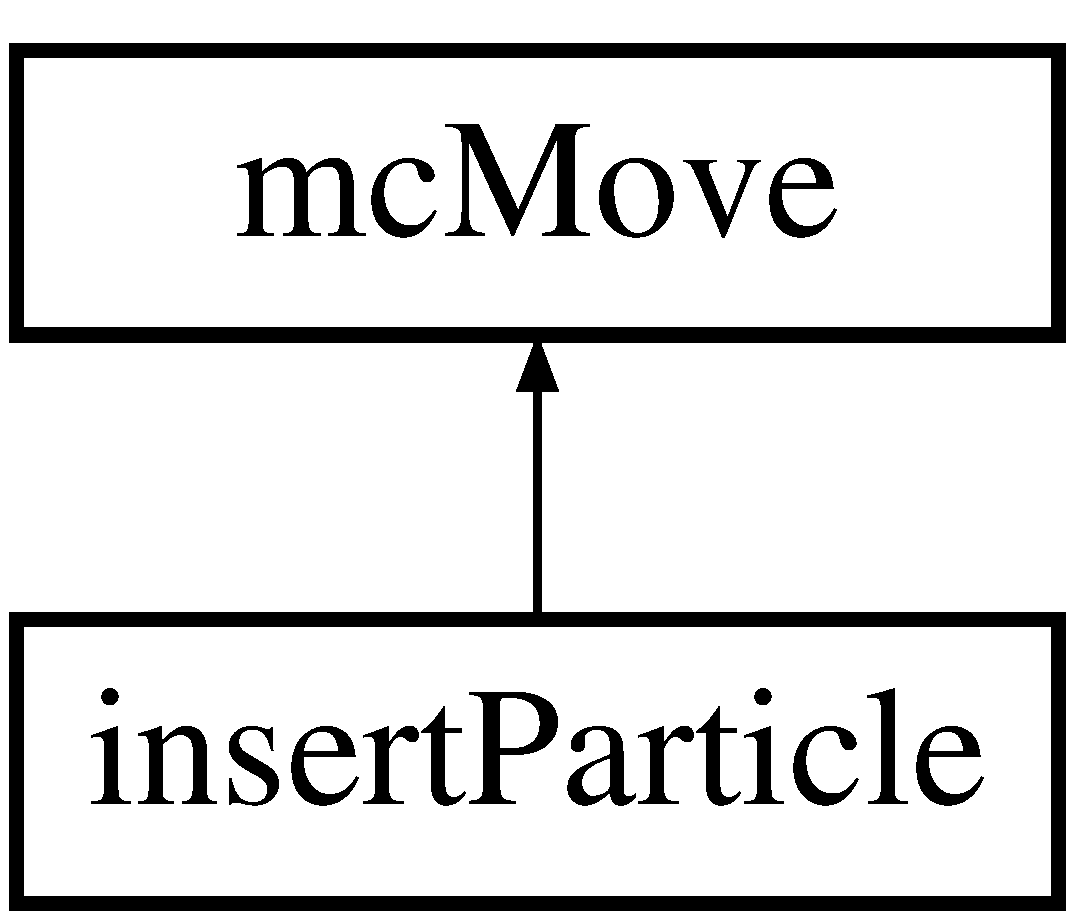
\includegraphics[height=2.000000cm]{classinsert_particle}
\end{center}
\end{figure}
\subsection*{Public Member Functions}
\begin{DoxyCompactItemize}
\item 
\hyperlink{classinsert_particle_adc56d982ad9d43537aea2744d13c3471}{insert\+Particle} ()
\item 
\hyperlink{classinsert_particle_af528d2c24fff7bea0701b014ae2fa5e4}{insert\+Particle} (const int type\+Index, const std\+::string tag)
\begin{DoxyCompactList}\small\item\em Instantiate a new move, also give a name which is the combination of auser-\/defined tag + the particle index it operates on. \end{DoxyCompactList}\item 
int \hyperlink{classinsert_particle_ad81c09b735d1acea65758242d5c5d595}{make} (\hyperlink{classsim_system}{sim\+System} \&sys)
\begin{DoxyCompactList}\small\item\em Insert a particle into the system. \end{DoxyCompactList}\end{DoxyCompactItemize}
\subsection*{Additional Inherited Members}


\subsection{Detailed Description}


Definition at line 12 of file insert.\+h.



\subsection{Constructor \& Destructor Documentation}
\hypertarget{classinsert_particle_adc56d982ad9d43537aea2744d13c3471}{}\index{insert\+Particle@{insert\+Particle}!insert\+Particle@{insert\+Particle}}
\index{insert\+Particle@{insert\+Particle}!insert\+Particle@{insert\+Particle}}
\subsubsection[{insert\+Particle()}]{\setlength{\rightskip}{0pt plus 5cm}insert\+Particle\+::insert\+Particle (
\begin{DoxyParamCaption}
{}
\end{DoxyParamCaption}
)\hspace{0.3cm}{\ttfamily [inline]}}\label{classinsert_particle_adc56d982ad9d43537aea2744d13c3471}


Definition at line 14 of file insert.\+h.


\begin{DoxyCode}
14 \{\};
\end{DoxyCode}
\hypertarget{classinsert_particle_af528d2c24fff7bea0701b014ae2fa5e4}{}\index{insert\+Particle@{insert\+Particle}!insert\+Particle@{insert\+Particle}}
\index{insert\+Particle@{insert\+Particle}!insert\+Particle@{insert\+Particle}}
\subsubsection[{insert\+Particle(const int type\+Index, const std\+::string tag)}]{\setlength{\rightskip}{0pt plus 5cm}insert\+Particle\+::insert\+Particle (
\begin{DoxyParamCaption}
\item[{const int}]{type\+Index, }
\item[{const std\+::string}]{tag}
\end{DoxyParamCaption}
)\hspace{0.3cm}{\ttfamily [inline]}}\label{classinsert_particle_af528d2c24fff7bea0701b014ae2fa5e4}


Instantiate a new move, also give a name which is the combination of auser-\/defined tag + the particle index it operates on. 



Definition at line 15 of file insert.\+h.



References mc\+Move\+::name\+\_\+, and mc\+Move\+::type\+Index\+\_\+.



\subsection{Member Function Documentation}
\hypertarget{classinsert_particle_ad81c09b735d1acea65758242d5c5d595}{}\index{insert\+Particle@{insert\+Particle}!make@{make}}
\index{make@{make}!insert\+Particle@{insert\+Particle}}
\subsubsection[{make(sim\+System \&sys)}]{\setlength{\rightskip}{0pt plus 5cm}int insert\+Particle\+::make (
\begin{DoxyParamCaption}
\item[{{\bf sim\+System} \&}]{sys}
\end{DoxyParamCaption}
)\hspace{0.3cm}{\ttfamily [virtual]}}\label{classinsert_particle_ad81c09b735d1acea65758242d5c5d595}


Insert a particle into the system. 

All other information is stored in the \hyperlink{classsim_system}{sim\+System} object.


\begin{DoxyParams}[1]{Parameters}
\mbox{\tt in}  & {\em sys} & System object to attempt to insert a particle into.\\
\hline
\end{DoxyParams}
\begin{DoxyReturn}{Returns}
M\+O\+V\+E\+\_\+\+S\+U\+C\+C\+E\+S\+S if inserted a particle, otherwise M\+O\+V\+E\+\_\+\+F\+A\+I\+L\+U\+R\+E if did not. Will throw exceptions if there was an error. 
\end{DoxyReturn}


Implements \hyperlink{classmc_move_a2e377a628f9ecee5422fc8967d4924eb}{mc\+Move}.



Definition at line 10 of file insert.\+cpp.



References sim\+System\+::beta(), sim\+System\+::box(), calculate\+Bias(), sim\+System\+::get\+Neighbor\+Positions(), sim\+System\+::get\+Tot\+N(), sim\+System\+::get\+W\+A\+L\+A\+Bias(), sim\+System\+::increment\+Energy(), sim\+System\+::insert\+Atom(), sim\+System\+::max\+Species(), M\+O\+V\+E\+\_\+\+F\+A\+I\+L\+U\+R\+E, M\+O\+V\+E\+\_\+\+S\+U\+C\+C\+E\+S\+S, sim\+System\+::mu(), sim\+System\+::n\+Species(), sim\+System\+::num\+Species, atom\+::pos, sim\+System\+::ppot, rng(), R\+N\+G\+\_\+\+S\+E\+E\+D, sim\+System\+::tot\+N\+Max(), mc\+Move\+::type\+Index\+\_\+, wala\+::update(), sim\+System\+::use\+W\+A\+L\+A, and custom\+Exception\+::what().


\begin{DoxyCode}
10                                         \{
11     \textcolor{comment}{// check if at upper bound for this specific species type}
12     \textcolor{keywordflow}{if} (sys.\hyperlink{classsim_system_a9eea865e6dc1cff377b1e79c4d9c23f0}{numSpecies}[\hyperlink{classmc_move_acb731965547b0326ef318ec96da8b46a}{typeIndex\_}] >= sys.\hyperlink{classsim_system_a93259b517f449f1ac610d132ac66b551}{maxSpecies}(
      \hyperlink{classmc_move_acb731965547b0326ef318ec96da8b46a}{typeIndex\_})) \{
13         \textcolor{keywordflow}{return} \hyperlink{moves_8h_a9832cf5fcfa8c0894545b591c9908e39}{MOVE\_FAILURE};
14     \}
15     \textcolor{comment}{// also check if at upper bound for total number of atoms}
16     \textcolor{keywordflow}{if} (sys.\hyperlink{classsim_system_a37dd827f4057049763351510147b9f1d}{getTotN}() >= sys.\hyperlink{classsim_system_aee2c65ecb43a35c0c4d070cdb45f7dc0}{totNMax}()) \{
17                 \textcolor{keywordflow}{return} \hyperlink{moves_8h_a9832cf5fcfa8c0894545b591c9908e39}{MOVE\_FAILURE};
18     \}
19     
20                 \textcolor{comment}{// attempt to insert a new one}
21     \hyperlink{classatom}{atom} newAtom;
22     \textcolor{keyword}{const} std::vector < double > box = sys.\hyperlink{classsim_system_a8bff9dfb95b1b09a0fab2c1c485ade07}{box}();
23     \textcolor{keywordtype}{double} V = 1.0;
24     \textcolor{keywordflow}{for} (\textcolor{keywordtype}{unsigned} \textcolor{keywordtype}{int} i = 0; i < box.size(); ++i) \{
25         newAtom.\hyperlink{classatom_a3ae5f4880e7831d8b2c9fda72b4eb24a}{pos}[i] = \hyperlink{utilities_8cpp_a0f9542af4b475ac79cb679d7a8d14db0}{rng} (&\hyperlink{global_8h_a3f4e4ea24d5a5c66feae55d1f329c884}{RNG\_SEED}) * box[i];
26         V *= box[i];
27     \}
28     
29     \textcolor{comment}{// compute energy to insert}
30     \textcolor{keywordtype}{double} insEnergy = 0.0;
31     \textcolor{keywordflow}{for} (\textcolor{keywordtype}{unsigned} \textcolor{keywordtype}{int} spec = 0; spec < sys.\hyperlink{classsim_system_ab5e2e9b6204de15520302fe1d51688dd}{nSpecies}(); ++spec) \{
32                 \textcolor{comment}{// get positions of neighboring atoms around newAtom}
33                 std::vector < std::vector < double > > neighborPositions = sys.
      \hyperlink{classsim_system_a7ac49b2311cd8230df8d078a9d897b35}{getNeighborPositions}(spec, \hyperlink{classmc_move_acb731965547b0326ef318ec96da8b46a}{typeIndex\_}, &newAtom);
34         \textcolor{keywordflow}{for} (\textcolor{keywordtype}{unsigned} \textcolor{keywordtype}{int} i = 0; i < neighborPositions.size(); ++i) \{
35                                                 \textcolor{keywordflow}{try} \{
36                                                                 insEnergy += sys.
      \hyperlink{classsim_system_a8d6271751a62f61edcf57f773540a4a3}{ppot}[spec][\hyperlink{classmc_move_acb731965547b0326ef318ec96da8b46a}{typeIndex\_}]->energy(neighborPositions[i], newAtom.\hyperlink{classatom_a3ae5f4880e7831d8b2c9fda72b4eb24a}{pos}, box);        
37                                                 \} \textcolor{keywordflow}{catch} (\hyperlink{classcustom_exception}{customException}& ce) \{
38                                                                 std::string a = \textcolor{stringliteral}{"Cannot insert because of
       energy error: "}, b = ce.\hyperlink{classcustom_exception_aeb6ab5848b038adfc68fde86a512f691}{what}();
39                                                                 \textcolor{keywordflow}{throw} 
      \hyperlink{classcustom_exception}{customException} (a+b);
40                                                 \}
41         \}
42         \textcolor{comment}{// add tail correction to potential energy -- only enable for fluid phase simulations}
43 \textcolor{preprocessor}{#ifdef FLUID\_PHASE\_SIMULATIONS}
44         \textcolor{keywordflow}{if} (sys.\hyperlink{classsim_system_a8d6271751a62f61edcf57f773540a4a3}{ppot}[spec][\hyperlink{classmc_move_acb731965547b0326ef318ec96da8b46a}{typeIndex\_}]->useTailCorrection)\{
45                                                 insEnergy += sys.\hyperlink{classsim_system_a8d6271751a62f61edcf57f773540a4a3}{ppot}[spec][
      \hyperlink{classmc_move_acb731965547b0326ef318ec96da8b46a}{typeIndex\_}]->tailCorrection(sys.\hyperlink{classsim_system_a9eea865e6dc1cff377b1e79c4d9c23f0}{numSpecies}[spec]/V);
46                                 \}
47 \textcolor{preprocessor}{#endif}
48     \}
49     
50     \textcolor{comment}{// biasing}
51     \textcolor{keyword}{const} \textcolor{keywordtype}{double} p\_u = V/(sys.\hyperlink{classsim_system_a9eea865e6dc1cff377b1e79c4d9c23f0}{numSpecies}[\hyperlink{classmc_move_acb731965547b0326ef318ec96da8b46a}{typeIndex\_}]+1.0)*exp(sys.
      \hyperlink{classsim_system_a3eeec9678902f8d7fce4dad6064aaf4c}{beta}()*(sys.\hyperlink{classsim_system_af1e3f5320aff976a448647244d5950d1}{mu}(typeIndex\_) - insEnergy));
52     \textcolor{keywordtype}{int} nTotFinal = sys.\hyperlink{classsim_system_a37dd827f4057049763351510147b9f1d}{getTotN}() + 1;
53     \textcolor{keywordtype}{double} bias = \hyperlink{system_8cpp_ab912bbb9fc9045954cf1b3ccb286a55c}{calculateBias}(sys, nTotFinal, p\_u);
54    
55                 \textcolor{comment}{// metropolis criterion}
56                 \textcolor{keywordflow}{if} (\hyperlink{utilities_8cpp_a0f9542af4b475ac79cb679d7a8d14db0}{rng} (&\hyperlink{global_8h_a3f4e4ea24d5a5c66feae55d1f329c884}{RNG\_SEED}) < p\_u*bias) \{
57         \textcolor{keywordflow}{try} \{
58             sys.\hyperlink{classsim_system_a6c1e86f585f3a52aa82b6394ffbf1c6a}{insertAtom}(typeIndex\_, &newAtom);
59         \} \textcolor{keywordflow}{catch} (\hyperlink{classcustom_exception}{customException} &ce) \{
60             std::string a = \textcolor{stringliteral}{"Failed to insert atom: "}, b = ce.\hyperlink{classcustom_exception_aeb6ab5848b038adfc68fde86a512f691}{what}();
61             \textcolor{keywordflow}{throw} \hyperlink{classcustom_exception}{customException} (a+b);
62         \}
63                                 sys.\hyperlink{classsim_system_a6ad31c08955b80873f865b3069618dcb}{incrementEnergy}(insEnergy);
64                                 
65                                 \textcolor{comment}{// update Wang-Landau bias, if used}
66                                 \textcolor{keywordflow}{if} (sys.\hyperlink{classsim_system_aa83b00006b3919fb6e13f1bdeadece6a}{useWALA}) \{
67                                                 sys.\hyperlink{classsim_system_a7cb5049de8b0988349e89e30e4000407}{getWALABias}()->
      \hyperlink{classwala_a5eb2622be6a9e89f5e59ba0b15aca4bd}{update}(sys.\hyperlink{classsim_system_a37dd827f4057049763351510147b9f1d}{getTotN}());
68                                 \}
69                                 
70         \textcolor{keywordflow}{return} \hyperlink{moves_8h_ae8285cbddc5d21f73f49dcbad82a775a}{MOVE\_SUCCESS};
71     \}
72     
73                 \textcolor{comment}{// update Wang-Landau bias (even if moved failed), if used}
74                 \textcolor{keywordflow}{if} (sys.\hyperlink{classsim_system_aa83b00006b3919fb6e13f1bdeadece6a}{useWALA}) \{
75                                 sys.\hyperlink{classsim_system_a7cb5049de8b0988349e89e30e4000407}{getWALABias}()->\hyperlink{classwala_a5eb2622be6a9e89f5e59ba0b15aca4bd}{update}(sys.
      \hyperlink{classsim_system_a37dd827f4057049763351510147b9f1d}{getTotN}());
76                 \}
77                 
78                 \textcolor{keywordflow}{return} \hyperlink{moves_8h_a9832cf5fcfa8c0894545b591c9908e39}{MOVE\_FAILURE};
79 \}
\end{DoxyCode}


The documentation for this class was generated from the following files\+:\begin{DoxyCompactItemize}
\item 
/\+Users/nam4/\+Desktop/omcs/src/\hyperlink{insert_8h}{insert.\+h}\item 
/\+Users/nam4/\+Desktop/omcs/src/\hyperlink{insert_8cpp}{insert.\+cpp}\end{DoxyCompactItemize}

\hypertarget{classlennard_jones}{\section{lennard\-Jones Class Reference}
\label{classlennard_jones}\index{lennard\-Jones@{lennard\-Jones}}
}


Lennard-\/\-Jones Potential Parameters should be specified in the following order\-: \{ epsilon, sigma, r\-\_\-cut, u\-\_\-shift, Mtot \}.  




{\ttfamily \#include $<$potentials.\-h$>$}

Inheritance diagram for lennard\-Jones\-:\begin{figure}[H]
\begin{center}
\leavevmode
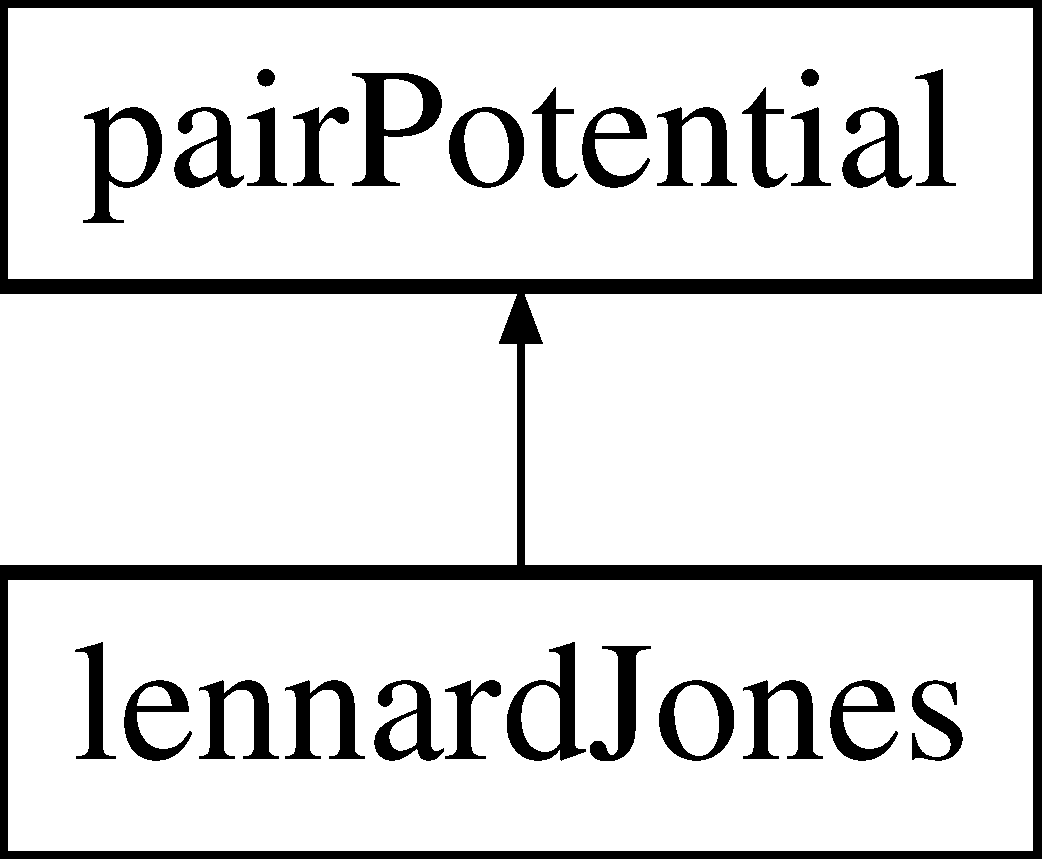
\includegraphics[height=2.000000cm]{classlennard_jones}
\end{center}
\end{figure}
\subsection*{Public Member Functions}
\begin{DoxyCompactItemize}
\item 
\hyperlink{classlennard_jones_aa05d64fac84629b8bfbbc1387a41119b}{$\sim$lennard\-Jones} ()
\item 
void \hyperlink{classlennard_jones_a5b4c41df05048ce99bffb9f27733100a}{set\-Parameters} (const std\-::vector$<$ double $>$ params)
\begin{DoxyCompactList}\small\item\em Set the parameters in the Lennard-\/\-Jones equation. \end{DoxyCompactList}\item 
double \hyperlink{classlennard_jones_a1be571dbb8f547f1bddaf76697fcad19}{energy} (const \hyperlink{classatom}{atom} $\ast$a1, const \hyperlink{classatom}{atom} $\ast$a2, const std\-::vector$<$ double $>$ \&box)
\begin{DoxyCompactList}\small\item\em Return the energy of two particles. \end{DoxyCompactList}\item 
double \hyperlink{classlennard_jones_a4518a7a9970c1fbed2f2abcf0ceebbfc}{tail\-Correction} (const double rho\-Bath)
\begin{DoxyCompactList}\small\item\em Calculate the tail correction with the approximation g(r) = 1 for r\-\_\-\{cut\} $>$ 1 as explained in Frenkel \& Smit in eq. \end{DoxyCompactList}\item 
double \hyperlink{classlennard_jones_a6ab5b04c385544da0de985e9635a6e8c}{rcut} ()
\begin{DoxyCompactList}\small\item\em Return the value of r\-\_\-\{cut\} for this potential. \end{DoxyCompactList}\end{DoxyCompactItemize}
\subsection*{Additional Inherited Members}


\subsection{Detailed Description}
Lennard-\/\-Jones Potential Parameters should be specified in the following order\-: \{ epsilon, sigma, r\-\_\-cut, u\-\_\-shift, Mtot \}. 

Definition at line 42 of file potentials.\-h.



\subsection{Constructor \& Destructor Documentation}
\hypertarget{classlennard_jones_aa05d64fac84629b8bfbbc1387a41119b}{\index{lennard\-Jones@{lennard\-Jones}!$\sim$lennard\-Jones@{$\sim$lennard\-Jones}}
\index{$\sim$lennard\-Jones@{$\sim$lennard\-Jones}!lennardJones@{lennard\-Jones}}
\subsubsection[{$\sim$lennard\-Jones}]{\setlength{\rightskip}{0pt plus 5cm}lennard\-Jones\-::$\sim$lennard\-Jones (
\begin{DoxyParamCaption}
{}
\end{DoxyParamCaption}
)\hspace{0.3cm}{\ttfamily [inline]}}}\label{classlennard_jones_aa05d64fac84629b8bfbbc1387a41119b}


Definition at line 44 of file potentials.\-h.


\begin{DoxyCode}
44 \{;\}
\end{DoxyCode}


\subsection{Member Function Documentation}
\hypertarget{classlennard_jones_a1be571dbb8f547f1bddaf76697fcad19}{\index{lennard\-Jones@{lennard\-Jones}!energy@{energy}}
\index{energy@{energy}!lennardJones@{lennard\-Jones}}
\subsubsection[{energy}]{\setlength{\rightskip}{0pt plus 5cm}double lennard\-Jones\-::energy (
\begin{DoxyParamCaption}
\item[{const {\bf atom} $\ast$}]{a1, }
\item[{const {\bf atom} $\ast$}]{a2, }
\item[{const std\-::vector$<$ double $>$ \&}]{box}
\end{DoxyParamCaption}
)\hspace{0.3cm}{\ttfamily [virtual]}}}\label{classlennard_jones_a1be571dbb8f547f1bddaf76697fcad19}


Return the energy of two particles. 

\[ U(r) = 4 \epsilon \left( \left \frac{ \sigma }{ r } \right)^{12} - \left( \frac{ sigma }{ r } \right)^6 \right) + U_{shift} \quad r < r_{cut} \]


\begin{DoxyParams}[1]{Parameters}
\mbox{\tt in}  & {\em a1} & Atom 1 \\
\hline
\mbox{\tt in}  & {\em a2} & Atom 2 \\
\hline
\mbox{\tt in}  & {\em box} & Simulation box dimensions\\
\hline
\end{DoxyParams}
\begin{DoxyReturn}{Returns}
U(r) 
\end{DoxyReturn}


Implements \hyperlink{classpair_potential_a2b1e50ef9b6e50b01d89d31d5460ad76}{pair\-Potential}.



Definition at line 230 of file potentials.\-cpp.



References atom\-::m\-State, pair\-Potential\-::params\-\_\-, pair\-Potential\-::params\-Are\-Set\-\_\-, pbc\-Dist2(), and atom\-::pos.


\begin{DoxyCode}
230                                                                                             \{
231     \textcolor{keywordflow}{if} (!\hyperlink{classpair_potential_a635755c0a952bfc05a4cfae230c3dbd2}{paramsAreSet\_}) \{
232         \textcolor{keywordflow}{throw} \hyperlink{classcustom_exception}{customException} (\textcolor{stringliteral}{"For lennardJones parameters not set"});
233     \}
234 
235     \textcolor{keyword}{const} \textcolor{keywordtype}{double} r\_sq = \hyperlink{utilities_8cpp_abb1db3a8a3ac46e044bbe7b2c5684c0a}{pbcDist2}(a1->\hyperlink{classatom_a3ae5f4880e7831d8b2c9fda72b4eb24a}{pos}, a2->\hyperlink{classatom_a3ae5f4880e7831d8b2c9fda72b4eb24a}{pos}, box);
236 
237     \textcolor{comment}{// only one of these atoms (at most) should be "partially" inserted}
238     \textcolor{keywordtype}{int} mState = 0;
239     \textcolor{keywordflow}{if} (a1->\hyperlink{classatom_a3cb00c0c5b7533657e05af6ff4a42740}{mState} != 0) \{
240         mState = a1->\hyperlink{classatom_a3cb00c0c5b7533657e05af6ff4a42740}{mState};
241     \}
242     \textcolor{keywordflow}{if} (a2->\hyperlink{classatom_a3cb00c0c5b7533657e05af6ff4a42740}{mState} != 0) \{
243         mState = a2->\hyperlink{classatom_a3cb00c0c5b7533657e05af6ff4a42740}{mState};
244     \}
245 
246     \textcolor{keywordtype}{double} r2 = (sigmaM\_[mState]*sigmaM\_[mState]/r\_sq), r6 = r2*r2*r2, r12 = r6*r6;
247     \textcolor{keywordflow}{if} (r\_sq < \hyperlink{classpair_potential_abf8ec8af983d6e9960bd149da099e883}{params\_}[2]*\hyperlink{classpair_potential_abf8ec8af983d6e9960bd149da099e883}{params\_}[2]) \{
248         \textcolor{keywordflow}{return} 4.0*epsM\_[mState]*(r12 - r6) + uShiftM\_[mState];
249     \} \textcolor{keywordflow}{else} \{
250         \textcolor{keywordflow}{return} 0.0;
251     \}
252 \}
\end{DoxyCode}
\hypertarget{classlennard_jones_a6ab5b04c385544da0de985e9635a6e8c}{\index{lennard\-Jones@{lennard\-Jones}!rcut@{rcut}}
\index{rcut@{rcut}!lennardJones@{lennard\-Jones}}
\subsubsection[{rcut}]{\setlength{\rightskip}{0pt plus 5cm}double lennard\-Jones\-::rcut (
\begin{DoxyParamCaption}
{}
\end{DoxyParamCaption}
)\hspace{0.3cm}{\ttfamily [virtual]}}}\label{classlennard_jones_a6ab5b04c385544da0de985e9635a6e8c}


Return the value of r\-\_\-\{cut\} for this potential. 

\begin{DoxyReturn}{Returns}
rcut 
\end{DoxyReturn}


Implements \hyperlink{classpair_potential_abf4f8d231c5e2e36d72916d33dcd75f0}{pair\-Potential}.



Definition at line 278 of file potentials.\-cpp.



References pair\-Potential\-::params\-\_\-, and pair\-Potential\-::params\-Are\-Set\-\_\-.


\begin{DoxyCode}
278                            \{
279     \textcolor{keywordflow}{if} (!\hyperlink{classpair_potential_a635755c0a952bfc05a4cfae230c3dbd2}{paramsAreSet\_}) \{
280         \textcolor{keywordflow}{throw} \hyperlink{classcustom_exception}{customException} (\textcolor{stringliteral}{"For lennardJones parameters not set"});
281     \} \textcolor{keywordflow}{else} \{
282         \textcolor{keywordflow}{return} \hyperlink{classpair_potential_abf8ec8af983d6e9960bd149da099e883}{params\_}[2];
283     \}
284 \}
\end{DoxyCode}
\hypertarget{classlennard_jones_a5b4c41df05048ce99bffb9f27733100a}{\index{lennard\-Jones@{lennard\-Jones}!set\-Parameters@{set\-Parameters}}
\index{set\-Parameters@{set\-Parameters}!lennardJones@{lennard\-Jones}}
\subsubsection[{set\-Parameters}]{\setlength{\rightskip}{0pt plus 5cm}void lennard\-Jones\-::set\-Parameters (
\begin{DoxyParamCaption}
\item[{const std\-::vector$<$ double $>$}]{params}
\end{DoxyParamCaption}
)\hspace{0.3cm}{\ttfamily [virtual]}}}\label{classlennard_jones_a5b4c41df05048ce99bffb9f27733100a}


Set the parameters in the Lennard-\/\-Jones equation. 


\begin{DoxyParams}[1]{Parameters}
\mbox{\tt in}  & {\em params} & Vector of inputs\-: \{epsilon, sigma, r\-\_\-cut, u\-\_\-shift, Mtot\} \\
\hline
\end{DoxyParams}


Implements \hyperlink{classpair_potential_ad4b237646f9de2ae9f95cc9350564bc5}{pair\-Potential}.



Definition at line 155 of file potentials.\-cpp.



References pair\-Potential\-::params\-\_\-, pair\-Potential\-::params\-Are\-Set\-\_\-, and pair\-Potential\-::use\-Tail\-Correction.


\begin{DoxyCode}
155                                                                    \{
156     \textcolor{keywordflow}{if} (params.size() != 5) \{
157         \textcolor{keywordflow}{throw} \hyperlink{classcustom_exception}{customException} (\textcolor{stringliteral}{"For lennardJones must specify 5 parameters: epsilon, sigma,
       r\_cut, u\_shift, Mtot"});
158     \} \textcolor{keywordflow}{else} \{
159         \textcolor{keywordflow}{if} (params[0] < 0) \{
160             \textcolor{keywordflow}{throw} \hyperlink{classcustom_exception}{customException} (\textcolor{stringliteral}{"For lennardJones, epsilon >= 0"});
161         \}
162         \textcolor{keywordflow}{if} (params[1] < 0) \{
163             \textcolor{keywordflow}{throw} \hyperlink{classcustom_exception}{customException} (\textcolor{stringliteral}{"For lennardJones, sigma >= 0"});
164         \}
165         \textcolor{keywordflow}{if} (params[2] < 0) \{
166             \textcolor{keywordflow}{throw} \hyperlink{classcustom_exception}{customException} (\textcolor{stringliteral}{"For lennardJones, r\_cut >= 0"});
167         \}
168         \textcolor{keywordflow}{if} (\textcolor{keywordtype}{int}(params[4]) < 1) \{
169             \textcolor{keywordflow}{throw} \hyperlink{classcustom_exception}{customException} (\textcolor{stringliteral}{"For lennardJones, total expanded ensemble states, Mtot
       >= 1"});
170         \}
171 
172         \hyperlink{classpair_potential_a635755c0a952bfc05a4cfae230c3dbd2}{paramsAreSet\_} = \textcolor{keyword}{true};
173         \hyperlink{classpair_potential_abf8ec8af983d6e9960bd149da099e883}{params\_} = params;
174 
175         \hyperlink{classpair_potential_ab4b4538a7e13771f50a29aaac2443037}{useTailCorrection} = \textcolor{keyword}{true};
176 
177         \textcolor{comment}{// use a "constant volume" scheme to distribute the stages}
178         sigmaM\_.resize(\textcolor{keywordtype}{int}(params[4]), 0);
179         \textcolor{keywordflow}{for} (\textcolor{keywordtype}{int} i = 0; i < sigmaM\_.size(); ++i) \{
180             \textcolor{keywordflow}{if} (i == 0) \{
181                 \textcolor{comment}{// fully inserted}
182                 sigmaM\_[i] = params[1];
183             \} \textcolor{keywordflow}{else} \{
184                 \textcolor{comment}{// use volume scaling so each stage is separated from its neighbors by the same dV}
185                 \textcolor{keywordtype}{double} lastSigma = 0;
186                 \textcolor{keywordflow}{if} (i == 1) \{
187                     lastSigma = 0;
188                 \} \textcolor{keywordflow}{else} \{
189                     lastSigma = sigmaM\_[i-1];
190                 \}
191                 sigmaM\_[i] = pow(params[1]*params[1]*params[1]/(8.0*\textcolor{keywordtype}{int}(params[4])) + lastSigma*lastSigma*
      lastSigma, 1./3.);
192             \}
193         \}
194 
195         \textcolor{comment}{// scale energy linearly across the stages}
196         epsM\_.resize(\textcolor{keywordtype}{int}(params[4]), 0);
197         \textcolor{keywordflow}{for} (\textcolor{keywordtype}{int} i = 0; i < epsM\_.size(); ++i) \{
198             \textcolor{keywordflow}{if} (i == 0) \{
199                 \textcolor{comment}{// fully inserted}
200                 epsM\_[i] = params[0];
201             \} \textcolor{keywordflow}{else} \{
202                 epsM\_[i] = i*(params[0]/int(params[4]));
203             \}
204         \}
205 
206         \textcolor{comment}{// scale energy linearly across the stages}
207         uShiftM\_.resize(\textcolor{keywordtype}{int}(params[4]), 0);
208         \textcolor{keywordflow}{for} (\textcolor{keywordtype}{int} i = 0; i < epsM\_.size(); ++i) \{
209             \textcolor{keywordflow}{if} (i == 0) \{
210                 \textcolor{comment}{// fully inserted}
211                 uShiftM\_[i] = params[3];
212             \} \textcolor{keywordflow}{else} \{
213                 uShiftM\_[i] = i*(params[3]/int(params[4]));
214             \}
215         \}
216     \}
217 \}
\end{DoxyCode}
\hypertarget{classlennard_jones_a4518a7a9970c1fbed2f2abcf0ceebbfc}{\index{lennard\-Jones@{lennard\-Jones}!tail\-Correction@{tail\-Correction}}
\index{tail\-Correction@{tail\-Correction}!lennardJones@{lennard\-Jones}}
\subsubsection[{tail\-Correction}]{\setlength{\rightskip}{0pt plus 5cm}double lennard\-Jones\-::tail\-Correction (
\begin{DoxyParamCaption}
\item[{const double}]{rho\-Bath}
\end{DoxyParamCaption}
)\hspace{0.3cm}{\ttfamily [virtual]}}}\label{classlennard_jones_a4518a7a9970c1fbed2f2abcf0ceebbfc}


Calculate the tail correction with the approximation g(r) = 1 for r\-\_\-\{cut\} $>$ 1 as explained in Frenkel \& Smit in eq. 

(3.\-2.\-5). Tail corrections only account for number of fully inserted particles so I have chosen not to scale this part of the energy with expanded ensemble stage.


\begin{DoxyParams}[1]{Parameters}
\mbox{\tt in}  & {\em rho\-Bath} & Number density of the surrounding fluid\\
\hline
\end{DoxyParams}
\begin{DoxyReturn}{Returns}
U\-\_\-tail 
\end{DoxyReturn}


Implements \hyperlink{classpair_potential_a5387d21d8d487d1d42e9eaf7cae9175b}{pair\-Potential}.



Definition at line 263 of file potentials.\-cpp.



References pair\-Potential\-::params\-\_\-, and P\-I.


\begin{DoxyCode}
263                                                         \{
264     \textcolor{keywordflow}{if} (rhoBath < 0) \{
265         \textcolor{keywordflow}{return} 0;
266     \}
267     \textcolor{keyword}{const} \textcolor{keywordtype}{double} r3 = (\hyperlink{classpair_potential_abf8ec8af983d6e9960bd149da099e883}{params\_}[1]*\hyperlink{classpair_potential_abf8ec8af983d6e9960bd149da099e883}{params\_}[1]*\hyperlink{classpair_potential_abf8ec8af983d6e9960bd149da099e883}{params\_}[1])/(
      \hyperlink{classpair_potential_abf8ec8af983d6e9960bd149da099e883}{params\_}[2]*\hyperlink{classpair_potential_abf8ec8af983d6e9960bd149da099e883}{params\_}[2]*\hyperlink{classpair_potential_abf8ec8af983d6e9960bd149da099e883}{params\_}[2]);
268     \textcolor{keyword}{const} \textcolor{keywordtype}{double} r9 = r3*r3*r3;
269 
270     \textcolor{keywordflow}{return} 2.0*(8.0/3.0*\hyperlink{global_8h_a598a3330b3c21701223ee0ca14316eca}{PI}*rhoBath*params\_[0]*params\_[1]*params\_[1]*params\_[1]*(r9/3.0 - r3));
271 \}
\end{DoxyCode}


The documentation for this class was generated from the following files\-:\begin{DoxyCompactItemize}
\item 
/home/nam4/\-Desktop/sandbox/\-F\-H\-M\-C\-Simulation/src/\hyperlink{potentials_8h}{potentials.\-h}\item 
/home/nam4/\-Desktop/sandbox/\-F\-H\-M\-C\-Simulation/src/\hyperlink{potentials_8cpp}{potentials.\-cpp}\end{DoxyCompactItemize}

\hypertarget{classmc_move}{}\section{mc\+Move Class Reference}
\label{classmc_move}\index{mc\+Move@{mc\+Move}}


Virtual base class for all Monte Carlo moves.  




{\ttfamily \#include $<$moves.\+h$>$}

Inheritance diagram for mc\+Move\+:\begin{figure}[H]
\begin{center}
\leavevmode
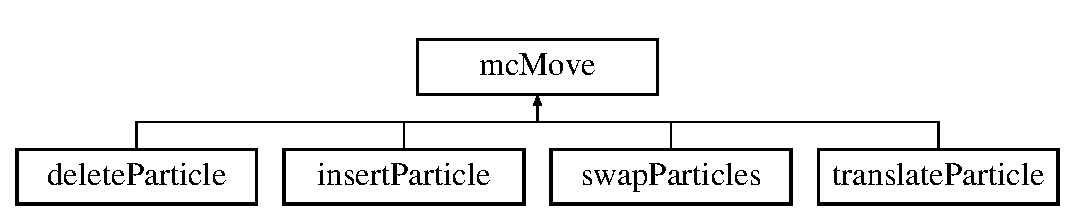
\includegraphics[height=2.000000cm]{classmc_move}
\end{center}
\end{figure}
\subsection*{Public Member Functions}
\begin{DoxyCompactItemize}
\item 
\hyperlink{classmc_move_a27a375cf5fcce904dc1ba6bc315b4e1c}{mc\+Move} ()
\item 
\hyperlink{classmc_move_ab0145ba0532e4d47156e2e4565d54c3f}{mc\+Move} (const int type\+Index, const std\+::string tag)
\item 
virtual \hyperlink{classmc_move_a3d9fd30dd96eebf857fa92f734d03bbc}{$\sim$mc\+Move} ()=0
\item 
virtual int \hyperlink{classmc_move_a2e377a628f9ecee5422fc8967d4924eb}{make} (\hyperlink{classsim_system}{sim\+System} \&sys)=0
\begin{DoxyCompactList}\small\item\em Make a M\+C move, return M\+O\+V\+E\+\_\+\+S\+U\+C\+C\+E\+S\+S or M\+O\+V\+E\+\_\+\+F\+A\+I\+L\+U\+R\+E. \end{DoxyCompactList}\item 
const int \hyperlink{classmc_move_aa96ed066866a2abf8b7039fd279d0f37}{what\+Type} ()
\begin{DoxyCompactList}\small\item\em Returns the index referring to the atom type this move operates on. \end{DoxyCompactList}\item 
const std\+::string \hyperlink{classmc_move_a7b068357010f8663674a7e70a7776ccd}{my\+Name} ()
\begin{DoxyCompactList}\small\item\em Return the name of this move. \end{DoxyCompactList}\end{DoxyCompactItemize}
\subsection*{Protected Attributes}
\begin{DoxyCompactItemize}
\item 
int \hyperlink{classmc_move_acb731965547b0326ef318ec96da8b46a}{type\+Index\+\_\+}
\begin{DoxyCompactList}\small\item\em Species index this move will operate on. \end{DoxyCompactList}\item 
std\+::string \hyperlink{classmc_move_ac18c307855e1cb5751bd6e079857a8c5}{name\+\_\+}
\begin{DoxyCompactList}\small\item\em Move name. \end{DoxyCompactList}\end{DoxyCompactItemize}


\subsection{Detailed Description}
Virtual base class for all Monte Carlo moves. 

Definition at line 17 of file moves.\+h.



\subsection{Constructor \& Destructor Documentation}
\hypertarget{classmc_move_a27a375cf5fcce904dc1ba6bc315b4e1c}{}\index{mc\+Move@{mc\+Move}!mc\+Move@{mc\+Move}}
\index{mc\+Move@{mc\+Move}!mc\+Move@{mc\+Move}}
\subsubsection[{mc\+Move()}]{\setlength{\rightskip}{0pt plus 5cm}mc\+Move\+::mc\+Move (
\begin{DoxyParamCaption}
{}
\end{DoxyParamCaption}
)\hspace{0.3cm}{\ttfamily [inline]}}\label{classmc_move_a27a375cf5fcce904dc1ba6bc315b4e1c}


Definition at line 19 of file moves.\+h.


\begin{DoxyCode}
19 \{\};
\end{DoxyCode}
\hypertarget{classmc_move_ab0145ba0532e4d47156e2e4565d54c3f}{}\index{mc\+Move@{mc\+Move}!mc\+Move@{mc\+Move}}
\index{mc\+Move@{mc\+Move}!mc\+Move@{mc\+Move}}
\subsubsection[{mc\+Move(const int type\+Index, const std\+::string tag)}]{\setlength{\rightskip}{0pt plus 5cm}mc\+Move\+::mc\+Move (
\begin{DoxyParamCaption}
\item[{const int}]{type\+Index, }
\item[{const std\+::string}]{tag}
\end{DoxyParamCaption}
)\hspace{0.3cm}{\ttfamily [inline]}}\label{classmc_move_ab0145ba0532e4d47156e2e4565d54c3f}


Definition at line 20 of file moves.\+h.



References name\+\_\+, and type\+Index\+\_\+.


\begin{DoxyCode}
20 \{ \hyperlink{classmc_move_acb731965547b0326ef318ec96da8b46a}{typeIndex\_} = typeIndex; \hyperlink{classmc_move_ac18c307855e1cb5751bd6e079857a8c5}{name\_} = tag + boost::lexical\_cast<std::string>(typeIndex); \}  
\end{DoxyCode}
\hypertarget{classmc_move_a3d9fd30dd96eebf857fa92f734d03bbc}{}\index{mc\+Move@{mc\+Move}!````~mc\+Move@{$\sim$mc\+Move}}
\index{````~mc\+Move@{$\sim$mc\+Move}!mc\+Move@{mc\+Move}}
\subsubsection[{$\sim$mc\+Move()=0}]{\setlength{\rightskip}{0pt plus 5cm}mc\+Move\+::$\sim$mc\+Move (
\begin{DoxyParamCaption}
{}
\end{DoxyParamCaption}
)\hspace{0.3cm}{\ttfamily [pure virtual]}}\label{classmc_move_a3d9fd30dd96eebf857fa92f734d03bbc}


Definition at line 3 of file moves.\+cpp.


\begin{DoxyCode}
3                  \{
4     ;
5 \}
\end{DoxyCode}


\subsection{Member Function Documentation}
\hypertarget{classmc_move_a2e377a628f9ecee5422fc8967d4924eb}{}\index{mc\+Move@{mc\+Move}!make@{make}}
\index{make@{make}!mc\+Move@{mc\+Move}}
\subsubsection[{make(sim\+System \&sys)=0}]{\setlength{\rightskip}{0pt plus 5cm}virtual int mc\+Move\+::make (
\begin{DoxyParamCaption}
\item[{{\bf sim\+System} \&}]{sys}
\end{DoxyParamCaption}
)\hspace{0.3cm}{\ttfamily [pure virtual]}}\label{classmc_move_a2e377a628f9ecee5422fc8967d4924eb}


Make a M\+C move, return M\+O\+V\+E\+\_\+\+S\+U\+C\+C\+E\+S\+S or M\+O\+V\+E\+\_\+\+F\+A\+I\+L\+U\+R\+E. 



Implemented in \hyperlink{classdelete_particle_a14f86dd27a82f571caa12af04e22eb1f}{delete\+Particle}, \hyperlink{classinsert_particle_ad81c09b735d1acea65758242d5c5d595}{insert\+Particle}, \hyperlink{classswap_particles_ad8ca574f8e5308b6f0a5f3c7c2799209}{swap\+Particles}, and \hyperlink{classtranslate_particle_a7ec5c9259f1aae3f7aefdb4db3ee5468}{translate\+Particle}.

\hypertarget{classmc_move_a7b068357010f8663674a7e70a7776ccd}{}\index{mc\+Move@{mc\+Move}!my\+Name@{my\+Name}}
\index{my\+Name@{my\+Name}!mc\+Move@{mc\+Move}}
\subsubsection[{my\+Name()}]{\setlength{\rightskip}{0pt plus 5cm}const std\+::string mc\+Move\+::my\+Name (
\begin{DoxyParamCaption}
{}
\end{DoxyParamCaption}
)\hspace{0.3cm}{\ttfamily [inline]}}\label{classmc_move_a7b068357010f8663674a7e70a7776ccd}


Return the name of this move. 



Definition at line 24 of file moves.\+h.



References name\+\_\+.

\hypertarget{classmc_move_aa96ed066866a2abf8b7039fd279d0f37}{}\index{mc\+Move@{mc\+Move}!what\+Type@{what\+Type}}
\index{what\+Type@{what\+Type}!mc\+Move@{mc\+Move}}
\subsubsection[{what\+Type()}]{\setlength{\rightskip}{0pt plus 5cm}const int mc\+Move\+::what\+Type (
\begin{DoxyParamCaption}
{}
\end{DoxyParamCaption}
)\hspace{0.3cm}{\ttfamily [inline]}}\label{classmc_move_aa96ed066866a2abf8b7039fd279d0f37}


Returns the index referring to the atom type this move operates on. 



Definition at line 23 of file moves.\+h.



References type\+Index\+\_\+.



\subsection{Member Data Documentation}
\hypertarget{classmc_move_ac18c307855e1cb5751bd6e079857a8c5}{}\index{mc\+Move@{mc\+Move}!name\+\_\+@{name\+\_\+}}
\index{name\+\_\+@{name\+\_\+}!mc\+Move@{mc\+Move}}
\subsubsection[{name\+\_\+}]{\setlength{\rightskip}{0pt plus 5cm}std\+::string mc\+Move\+::name\+\_\+\hspace{0.3cm}{\ttfamily [protected]}}\label{classmc_move_ac18c307855e1cb5751bd6e079857a8c5}


Move name. 



Definition at line 28 of file moves.\+h.



Referenced by delete\+Particle\+::delete\+Particle(), insert\+Particle\+::insert\+Particle(), mc\+Move(), my\+Name(), swap\+Particles\+::swap\+Particles(), and translate\+Particle\+::translate\+Particle().

\hypertarget{classmc_move_acb731965547b0326ef318ec96da8b46a}{}\index{mc\+Move@{mc\+Move}!type\+Index\+\_\+@{type\+Index\+\_\+}}
\index{type\+Index\+\_\+@{type\+Index\+\_\+}!mc\+Move@{mc\+Move}}
\subsubsection[{type\+Index\+\_\+}]{\setlength{\rightskip}{0pt plus 5cm}int mc\+Move\+::type\+Index\+\_\+\hspace{0.3cm}{\ttfamily [protected]}}\label{classmc_move_acb731965547b0326ef318ec96da8b46a}


Species index this move will operate on. 



Definition at line 27 of file moves.\+h.



Referenced by delete\+Particle\+::delete\+Particle(), insert\+Particle\+::insert\+Particle(), delete\+Particle\+::make(), translate\+Particle\+::make(), swap\+Particles\+::make(), insert\+Particle\+::make(), mc\+Move(), swap\+Particles\+::swap\+Particles(), translate\+Particle\+::translate\+Particle(), and what\+Type().



The documentation for this class was generated from the following files\+:\begin{DoxyCompactItemize}
\item 
/\+Users/nam4/\+Desktop/omcs/src/\hyperlink{moves_8h}{moves.\+h}\item 
/\+Users/nam4/\+Desktop/omcs/src/\hyperlink{moves_8cpp}{moves.\+cpp}\end{DoxyCompactItemize}

\hypertarget{classmoves}{\section{moves Class Reference}
\label{classmoves}\index{moves@{moves}}
}


Class that tracks and decides which moves whould be made.  




{\ttfamily \#include $<$mover.\-h$>$}

\subsection*{Public Member Functions}
\begin{DoxyCompactItemize}
\item 
\hyperlink{classmoves_a1964259b17a057e8b363736e42fca3e8}{moves} (const int M=1)
\begin{DoxyCompactList}\small\item\em Instantiate moves class. \end{DoxyCompactList}\item 
\hyperlink{classmoves_a00dfff19abe056adceb0ccf41778ee0f}{$\sim$moves} ()
\begin{DoxyCompactList}\small\item\em Destructor for moves class. \end{DoxyCompactList}\item 
void \hyperlink{classmoves_a3695f6a6d0128e2d0d76702f718accf8}{clear\-All} ()
\begin{DoxyCompactList}\small\item\em Clear all moves and related information from the class, but leaves M intact. \end{DoxyCompactList}\item 
void \hyperlink{classmoves_a7f023913b80bb62604b99f4dbf005c37}{make\-Move} (\hyperlink{classsim_system}{sim\-System} \&sys)
\begin{DoxyCompactList}\small\item\em Choose a move to make. \end{DoxyCompactList}\item 
void \hyperlink{classmoves_acc6415d4000f01b93235d1a533aa6880}{print} (const std\-::string filename)
\begin{DoxyCompactList}\small\item\em Print move information to file. \end{DoxyCompactList}\item 
void \hyperlink{classmoves_ab4583b3075f51cce55c3aeb84a58430d}{add\-Insert} (const int index, const double prob)
\begin{DoxyCompactList}\small\item\em Add insertion move. \end{DoxyCompactList}\item 
void \hyperlink{classmoves_ac4307636570c4d4bc07c4cba3887005e}{add\-Delete} (const int index, const double prob)
\begin{DoxyCompactList}\small\item\em Add deletion move. \end{DoxyCompactList}\item 
void \hyperlink{classmoves_a03cebfa2d8d1cecf253df573fdecc5d0}{add\-Swap} (const int index1, const int index2, const double prob)
\begin{DoxyCompactList}\small\item\em Add swap move. \end{DoxyCompactList}\item 
void \hyperlink{classmoves_a91bb7969368fdbb66920a11d79fe7552}{add\-Translate} (const int index, const double prob, const double max\-D, const std\-::vector$<$ double $>$ \&box)
\begin{DoxyCompactList}\small\item\em Add translate move. \end{DoxyCompactList}\item 
void \hyperlink{classmoves_ab603c6ce829075e3232ff41a7d5e2aab}{set\-M} (const int M)
\begin{DoxyCompactList}\small\item\em Set the value of M. \end{DoxyCompactList}\item 
int \hyperlink{classmoves_a57e814fe08153419f92a983cbf33796d}{get\-M} ()
\item 
std\-::vector$<$ std\-::vector\\*
$<$ double $>$ $>$ \hyperlink{classmoves_ad3e937628d85cdbbe02732648cb533e2}{report\-Move\-Statistics} ()
\begin{DoxyCompactList}\small\item\em Report the statistics on the success/failure of each move made so far. \end{DoxyCompactList}\item 
std\-::vector$<$ double $>$ \hyperlink{classmoves_a84f8198bd43c0f6b8b52dce3abdfa6a4}{report\-Probabilities} ()
\begin{DoxyCompactList}\small\item\em Echo the normalized probabilities of each move in the object. \end{DoxyCompactList}\end{DoxyCompactItemize}


\subsection{Detailed Description}
Class that tracks and decides which moves whould be made. 

However, it does N\-O\-T store the moves themselves so they should be fixed in memory elsewhere. 

Definition at line 20 of file mover.\-h.



\subsection{Constructor \& Destructor Documentation}
\hypertarget{classmoves_a1964259b17a057e8b363736e42fca3e8}{\index{moves@{moves}!moves@{moves}}
\index{moves@{moves}!moves@{moves}}
\subsubsection[{moves}]{\setlength{\rightskip}{0pt plus 5cm}moves\-::moves (
\begin{DoxyParamCaption}
\item[{const int}]{M = {\ttfamily 1}}
\end{DoxyParamCaption}
)}}\label{classmoves_a1964259b17a057e8b363736e42fca3e8}


Instantiate moves class. 


\begin{DoxyParams}{Parameters}
{\em in} & M Number of expanded ensemble stages for insert/delete moves \\
\hline
\end{DoxyParams}


Definition at line 8 of file mover.\-cpp.



References send\-Err(), set\-M(), S\-Y\-S\-\_\-\-F\-A\-I\-L\-U\-R\-E, and custom\-Exception\-::what().


\begin{DoxyCode}
8                          \{
9     \textcolor{keywordflow}{try} \{
10         \hyperlink{classmoves_ab603c6ce829075e3232ff41a7d5e2aab}{setM} (M);
11     \} \textcolor{keywordflow}{catch} (\hyperlink{classcustom_exception}{customException} &ce) \{
12         \hyperlink{utilities_8cpp_a6dacf3c3c19aa1e13a4d5a148fe5114e}{sendErr}(ce.\hyperlink{classcustom_exception_aeb6ab5848b038adfc68fde86a512f691}{what}());
13         exit(\hyperlink{global_8h_a428dfe1ef0a6ff4b1fdebf275f6aff2e}{SYS\_FAILURE});
14     \}
15 \}
\end{DoxyCode}
\hypertarget{classmoves_a00dfff19abe056adceb0ccf41778ee0f}{\index{moves@{moves}!$\sim$moves@{$\sim$moves}}
\index{$\sim$moves@{$\sim$moves}!moves@{moves}}
\subsubsection[{$\sim$moves}]{\setlength{\rightskip}{0pt plus 5cm}moves\-::$\sim$moves (
\begin{DoxyParamCaption}
{}
\end{DoxyParamCaption}
)}}\label{classmoves_a00dfff19abe056adceb0ccf41778ee0f}


Destructor for moves class. 



Definition at line 20 of file mover.\-cpp.


\begin{DoxyCode}
20                \{
21     ;
22 \}
\end{DoxyCode}


\subsection{Member Function Documentation}
\hypertarget{classmoves_ac4307636570c4d4bc07c4cba3887005e}{\index{moves@{moves}!add\-Delete@{add\-Delete}}
\index{add\-Delete@{add\-Delete}!moves@{moves}}
\subsubsection[{add\-Delete}]{\setlength{\rightskip}{0pt plus 5cm}void moves\-::add\-Delete (
\begin{DoxyParamCaption}
\item[{const int}]{index, }
\item[{const double}]{prob}
\end{DoxyParamCaption}
)}}\label{classmoves_ac4307636570c4d4bc07c4cba3887005e}


Add deletion move. 


\begin{DoxyParams}[1]{Parameters}
\mbox{\tt in}  & {\em index} & Particle index to operate on \\
\hline
\mbox{\tt in}  & {\em prob} & Probability \\
\hline
\end{DoxyParams}


Definition at line 95 of file mover.\-cpp.



References num\-To\-Str().



Referenced by set\-Moves().


\begin{DoxyCode}
95                                                          \{
96     \textcolor{keyword}{auto} om = std::make\_shared < deleteParticle > (index, \textcolor{stringliteral}{"delete"});
97     ownedMoves\_.push\_back(om);
98     \textcolor{keywordflow}{try} \{
99         addOn\_(ownedMoves\_.back()->changeN(), prob);
100     \} \textcolor{keywordflow}{catch} (std::exception &ex) \{
101         \textcolor{keyword}{const} std::string msg = ex.what();
102         \textcolor{keywordflow}{throw} \hyperlink{classcustom_exception}{customException} (\textcolor{stringliteral}{"Cannot add deletion move for species "}+
      \hyperlink{utilities_8h_ae6ed8fadf719af789711a7c0e99f44bc}{numToStr}(index+1)+\textcolor{stringliteral}{" : "}+msg);
103     \}
104 \}
\end{DoxyCode}
\hypertarget{classmoves_ab4583b3075f51cce55c3aeb84a58430d}{\index{moves@{moves}!add\-Insert@{add\-Insert}}
\index{add\-Insert@{add\-Insert}!moves@{moves}}
\subsubsection[{add\-Insert}]{\setlength{\rightskip}{0pt plus 5cm}void moves\-::add\-Insert (
\begin{DoxyParamCaption}
\item[{const int}]{index, }
\item[{const double}]{prob}
\end{DoxyParamCaption}
)}}\label{classmoves_ab4583b3075f51cce55c3aeb84a58430d}


Add insertion move. 


\begin{DoxyParams}[1]{Parameters}
\mbox{\tt in}  & {\em index} & Particle index to operate on \\
\hline
\mbox{\tt in}  & {\em prob} & Probability \\
\hline
\end{DoxyParams}


Definition at line 78 of file mover.\-cpp.



References num\-To\-Str().



Referenced by set\-Config(), and set\-Moves().


\begin{DoxyCode}
78                                                          \{
79     \textcolor{keyword}{auto} om = std::make\_shared < insertParticle > (index, \textcolor{stringliteral}{"insert"});
80     ownedMoves\_.push\_back(om);
81     \textcolor{keywordflow}{try} \{
82         addOn\_(ownedMoves\_.back()->changeN(), prob);
83     \} \textcolor{keywordflow}{catch} (std::exception &ex) \{
84         \textcolor{keyword}{const} std::string msg = ex.what();
85         \textcolor{keywordflow}{throw} \hyperlink{classcustom_exception}{customException} (\textcolor{stringliteral}{"Cannot add insertion move for species "}+
      \hyperlink{utilities_8h_ae6ed8fadf719af789711a7c0e99f44bc}{numToStr}(index+1)+\textcolor{stringliteral}{" : "}+msg);
86     \}
87 \}
\end{DoxyCode}
\hypertarget{classmoves_a03cebfa2d8d1cecf253df573fdecc5d0}{\index{moves@{moves}!add\-Swap@{add\-Swap}}
\index{add\-Swap@{add\-Swap}!moves@{moves}}
\subsubsection[{add\-Swap}]{\setlength{\rightskip}{0pt plus 5cm}void moves\-::add\-Swap (
\begin{DoxyParamCaption}
\item[{const int}]{index1, }
\item[{const int}]{index2, }
\item[{const double}]{prob}
\end{DoxyParamCaption}
)}}\label{classmoves_a03cebfa2d8d1cecf253df573fdecc5d0}


Add swap move. 


\begin{DoxyParams}[1]{Parameters}
\mbox{\tt in}  & {\em index1} & Particle index 1 to operate on \\
\hline
\mbox{\tt in}  & {\em index2} & Particle index 2 to operate on \\
\hline
\mbox{\tt in}  & {\em prob} & Probability \\
\hline
\end{DoxyParams}


Definition at line 113 of file mover.\-cpp.



References num\-To\-Str().



Referenced by set\-Moves().


\begin{DoxyCode}
113                                                                           \{
114     \textcolor{keyword}{auto} om = std::make\_shared < swapParticles > (index1, index2, \textcolor{stringliteral}{"swap"});
115     ownedMoves\_.push\_back(om);
116     \textcolor{keywordflow}{try} \{
117         addOn\_(ownedMoves\_.back()->changeN(), prob);
118     \} \textcolor{keywordflow}{catch} (std::exception &ex) \{
119         \textcolor{keyword}{const} std::string msg = ex.what();
120         \textcolor{keywordflow}{throw} \hyperlink{classcustom_exception}{customException} (\textcolor{stringliteral}{"Cannot add swap move for species pair ("}+
      \hyperlink{utilities_8h_ae6ed8fadf719af789711a7c0e99f44bc}{numToStr}(index1+1)+\textcolor{stringliteral}{","}+\hyperlink{utilities_8h_ae6ed8fadf719af789711a7c0e99f44bc}{numToStr}(index2+1)+\textcolor{stringliteral}{") : "}+msg);
121     \}
122 \}
\end{DoxyCode}
\hypertarget{classmoves_a91bb7969368fdbb66920a11d79fe7552}{\index{moves@{moves}!add\-Translate@{add\-Translate}}
\index{add\-Translate@{add\-Translate}!moves@{moves}}
\subsubsection[{add\-Translate}]{\setlength{\rightskip}{0pt plus 5cm}void moves\-::add\-Translate (
\begin{DoxyParamCaption}
\item[{const int}]{index, }
\item[{const double}]{prob, }
\item[{const double}]{max\-D, }
\item[{const std\-::vector$<$ double $>$ \&}]{box}
\end{DoxyParamCaption}
)}}\label{classmoves_a91bb7969368fdbb66920a11d79fe7552}


Add translate move. 


\begin{DoxyParams}[1]{Parameters}
\mbox{\tt in}  & {\em index} & Particle index to operate on \\
\hline
\mbox{\tt in}  & {\em prob} & Probability \\
\hline
\mbox{\tt in}  & {\em max\-D} & Maximium translation \\
\hline
\mbox{\tt in}  & {\em box} & Box dimensions \\
\hline
\end{DoxyParams}


Definition at line 132 of file mover.\-cpp.



References num\-To\-Str().



Referenced by set\-Moves().


\begin{DoxyCode}
132                                                                                                            
           \{
133     \textcolor{keyword}{auto} om = std::make\_shared < translateParticle > (index, \textcolor{stringliteral}{"translate"});
134     \textcolor{keywordflow}{try} \{
135         om->setMaxTranslation (maxD, box);
136         ownedMoves\_.push\_back(om);
137         addOn\_(ownedMoves\_.back()->changeN(), prob);
138     \} \textcolor{keywordflow}{catch} (std::exception &ex) \{
139         \textcolor{keyword}{const} std::string msg = ex.what();
140         \textcolor{keywordflow}{throw} \hyperlink{classcustom_exception}{customException} (\textcolor{stringliteral}{"Cannot add translation move for species "}+
      \hyperlink{utilities_8h_ae6ed8fadf719af789711a7c0e99f44bc}{numToStr}(index+1)+\textcolor{stringliteral}{" : "}+msg);
141     \}
142 \}
\end{DoxyCode}
\hypertarget{classmoves_a3695f6a6d0128e2d0d76702f718accf8}{\index{moves@{moves}!clear\-All@{clear\-All}}
\index{clear\-All@{clear\-All}!moves@{moves}}
\subsubsection[{clear\-All}]{\setlength{\rightskip}{0pt plus 5cm}void moves\-::clear\-All (
\begin{DoxyParamCaption}
{}
\end{DoxyParamCaption}
)}}\label{classmoves_a3695f6a6d0128e2d0d76702f718accf8}


Clear all moves and related information from the class, but leaves M intact. 



Definition at line 27 of file mover.\-cpp.



Referenced by set\-Moves().


\begin{DoxyCode}
27                       \{
28     normProbabilities\_.clear();
29     rawProbabilities\_.clear();
30     succeeded\_.clear();
31     attempted\_.clear();
32     ownedMoves\_.clear();
33 \}
\end{DoxyCode}
\hypertarget{classmoves_a57e814fe08153419f92a983cbf33796d}{\index{moves@{moves}!get\-M@{get\-M}}
\index{get\-M@{get\-M}!moves@{moves}}
\subsubsection[{get\-M}]{\setlength{\rightskip}{0pt plus 5cm}int moves\-::get\-M (
\begin{DoxyParamCaption}
{}
\end{DoxyParamCaption}
)\hspace{0.3cm}{\ttfamily [inline]}}}\label{classmoves_a57e814fe08153419f92a983cbf33796d}


Definition at line 33 of file mover.\-h.


\begin{DoxyCode}
33 \{ \textcolor{keywordflow}{return} M\_; \}
\end{DoxyCode}
\hypertarget{classmoves_a7f023913b80bb62604b99f4dbf005c37}{\index{moves@{moves}!make\-Move@{make\-Move}}
\index{make\-Move@{make\-Move}!moves@{moves}}
\subsubsection[{make\-Move}]{\setlength{\rightskip}{0pt plus 5cm}void moves\-::make\-Move (
\begin{DoxyParamCaption}
\item[{{\bf sim\-System} \&}]{sys}
\end{DoxyParamCaption}
)}}\label{classmoves_a7f023913b80bb62604b99f4dbf005c37}


Choose a move to make. 

If in an expanded ensemble, will restrict moves which change the number of particles to the atom type that is currently on partially in the system.


\begin{DoxyParams}[1]{Parameters}
\mbox{\tt in}  & {\em sys} & \hyperlink{classsim_system}{sim\-System} object to make a move in. \\
\hline
\end{DoxyParams}


Definition at line 191 of file mover.\-cpp.



References sim\-System\-::get\-Current\-M(), sim\-System\-::get\-Fractional\-Atom\-Type(), sim\-System\-::get\-Total\-M(), rng(), R\-N\-G\-\_\-\-S\-E\-E\-D, and custom\-Exception\-::what().



Referenced by perform\-Crossover(), perform\-T\-M\-M\-C(), and perform\-W\-A\-L\-A().


\begin{DoxyCode}
191                                     \{
192     \textcolor{keywordflow}{if} (sys.\hyperlink{classsim_system_aa4ad1afff101bb530e1590df05035276}{getTotalM}() != M\_) \{
193         \textcolor{keywordflow}{throw} \hyperlink{classcustom_exception}{customException} (\textcolor{stringliteral}{"Error, M in system different from M in moves class operating
       on the system"});
194     \}
195     \textcolor{keywordtype}{int} moveChosen = -1, succ = 0, mIndex = 0;
196     \textcolor{keywordtype}{bool} done = \textcolor{keyword}{false};
197     \textcolor{keywordflow}{while} (!done) \{
198         \textcolor{keyword}{const} \textcolor{keywordtype}{double} ran = \hyperlink{utilities_8cpp_a0f9542af4b475ac79cb679d7a8d14db0}{rng} (&\hyperlink{global_8h_a3f4e4ea24d5a5c66feae55d1f329c884}{RNG\_SEED});
199         \textcolor{keywordflow}{for} (\textcolor{keywordtype}{unsigned} \textcolor{keywordtype}{int} i = 0; i < normProbabilities\_.size(); ++i) \{
200             \textcolor{keywordflow}{if} (ran < normProbabilities\_[i]) \{
201                 \textcolor{keywordflow}{if} (sys.\hyperlink{classsim_system_aa4ad1afff101bb530e1590df05035276}{getTotalM}() > 1) \{
202                     \textcolor{comment}{// expanded ensemble has to check the moves because have to only work on the partially
       inserted atom}
203                     \textcolor{keywordflow}{if} ((ownedMoves\_[i]->changeN() == \textcolor{keyword}{true}) && (ownedMoves\_[i]->whatType() != sys.
      \hyperlink{classsim_system_a0500a9e84eecfbde7a98cf8a34f719d5}{getFractionalAtomType}()) && (sys.\hyperlink{classsim_system_a299fe4372e610b554eaaf5f5957b2dbc}{getCurrentM}() > 0)) \{
204                         \textcolor{comment}{// reject this choice because we must only insert/delete the type that is already
       partially inserted IFF we are *already* in a partially inserted state}
205                         \textcolor{comment}{// choose a new move}
206                         done = \textcolor{keyword}{false};
207                         \textcolor{keywordflow}{break};
208                     \} \textcolor{keywordflow}{else} \{
209                         \textcolor{comment}{// get M before move happens which can change the state of the system}
210                         \textcolor{keywordflow}{if} (ownedMoves\_[i]->changeN()) \{
211                             mIndex = sys.\hyperlink{classsim_system_a299fe4372e610b554eaaf5f5957b2dbc}{getCurrentM}();
212                         \}
213                         \textcolor{keywordflow}{try} \{
214                             succ = ownedMoves\_[i]->make(sys);
215                         \} \textcolor{keywordflow}{catch} (\hyperlink{classcustom_exception}{customException} &ce) \{
216                             std::string a = \textcolor{stringliteral}{"Failed to make a move properly: "};
217                             std::string b = ce.\hyperlink{classcustom_exception_aeb6ab5848b038adfc68fde86a512f691}{what}();
218                             \textcolor{keywordflow}{throw} \hyperlink{classcustom_exception}{customException}(a+b);
219                         \}
220                         done = \textcolor{keyword}{true};
221                         moveChosen = i;
222                         \textcolor{keywordflow}{break};
223                     \}
224                 \} \textcolor{keywordflow}{else} \{
225                     \textcolor{comment}{// without expanded ensemble, inserts/deletes can proceed unchecked}
226                     \textcolor{keywordflow}{try} \{
227                         succ = ownedMoves\_[i]->make(sys);
228                     \} \textcolor{keywordflow}{catch} (\hyperlink{classcustom_exception}{customException} &ce) \{
229                         std::string a = \textcolor{stringliteral}{"Failed to make a move properly: "};
230                         std::string b = ce.\hyperlink{classcustom_exception_aeb6ab5848b038adfc68fde86a512f691}{what}();
231                         \textcolor{keywordflow}{throw} \hyperlink{classcustom_exception}{customException}(a+b);
232                     \}
233                     done = \textcolor{keyword}{true};
234                     moveChosen = i;
235                     mIndex = 0;
236                     \textcolor{keywordflow}{break};
237                 \}
238             \}
239         \}
240     \}
241 
242     \textcolor{keywordflow}{if} (moveChosen < 0) \{
243         \textcolor{keywordflow}{throw} \hyperlink{classcustom_exception}{customException}(\textcolor{stringliteral}{"Failed to choose a move properly"});
244     \}
245 
246     attempted\_[moveChosen][mIndex] += 1.0;
247     succeeded\_[moveChosen][mIndex] += succ;
248 \}
\end{DoxyCode}
\hypertarget{classmoves_acc6415d4000f01b93235d1a533aa6880}{\index{moves@{moves}!print@{print}}
\index{print@{print}!moves@{moves}}
\subsubsection[{print}]{\setlength{\rightskip}{0pt plus 5cm}void moves\-::print (
\begin{DoxyParamCaption}
\item[{const std\-::string}]{filename}
\end{DoxyParamCaption}
)}}\label{classmoves_acc6415d4000f01b93235d1a533aa6880}


Print move information to file. 

Appends by default.


\begin{DoxyParams}[1]{Parameters}
\mbox{\tt in}  & {\em filename} & Name of file to print to. \\
\hline
\end{DoxyParams}


Definition at line 53 of file mover.\-cpp.



References get\-Time\-Stamp(), and report\-Move\-Statistics().



Referenced by perform\-Crossover(), perform\-T\-M\-M\-C(), and perform\-W\-A\-L\-A().


\begin{DoxyCode}
53                                            \{
54     std::ofstream statFile (filename.c\_str(), std::ofstream::out | std::ofstream::app);
55     std::vector < std::vector < double > > stats = \hyperlink{classmoves_ad3e937628d85cdbbe02732648cb533e2}{reportMoveStatistics}();
56     statFile << \textcolor{stringliteral}{"Time: "} << \hyperlink{utilities_8cpp_aa6d910bf51f18a75deb20c6f0fbba285}{getTimeStamp}() << std::endl;
57     statFile << \textcolor{stringliteral}{"---------- Move Statistics --------- "} << std::endl << \textcolor{stringliteral}{"Move\(\backslash\)t\(\backslash\)% Success"} << std::endl;
58     \textcolor{keywordflow}{for} (\textcolor{keywordtype}{unsigned} \textcolor{keywordtype}{int} i = 0; i < stats.size(); ++i) \{
59         \textcolor{keywordtype}{double} prod = 1.0;
60         \textcolor{keywordflow}{for} (\textcolor{keywordtype}{unsigned} \textcolor{keywordtype}{int} j = 0; j < stats[i].size(); ++j) \{
61             prod *= stats[i][j];
62             statFile << ownedMoves\_[i]->myName() << \textcolor{stringliteral}{" (from M = "} << j << \textcolor{stringliteral}{")\(\backslash\)t"} << stats[i][j]*100.0 << 
      std::endl;
63         \}
64         \textcolor{keywordflow}{if} (stats[i].size() > 1) \{
65             statFile << \textcolor{stringliteral}{"-------------------------------------\(\backslash\)nProduct of percentages (%) = "} << prod*100 
      << \textcolor{stringliteral}{"\(\backslash\)n-------------------------------------"} << std::endl;
66         \}
67     \}
68     statFile << \textcolor{stringliteral}{"------------------------------------ "} << std::endl;
69     statFile.close();
70 \}
\end{DoxyCode}
\hypertarget{classmoves_ad3e937628d85cdbbe02732648cb533e2}{\index{moves@{moves}!report\-Move\-Statistics@{report\-Move\-Statistics}}
\index{report\-Move\-Statistics@{report\-Move\-Statistics}!moves@{moves}}
\subsubsection[{report\-Move\-Statistics}]{\setlength{\rightskip}{0pt plus 5cm}std\-::vector$<$ std\-::vector$<$ double $>$ $>$ moves\-::report\-Move\-Statistics (
\begin{DoxyParamCaption}
{}
\end{DoxyParamCaption}
)}}\label{classmoves_ad3e937628d85cdbbe02732648cb533e2}


Report the statistics on the success/failure of each move made so far. 

If the move changes total number of particles in the system, there is a column for each expanded state it traverses.

\begin{DoxyReturn}{Returns}
ans Number of Success / Total Attempts for each move 
\end{DoxyReturn}


Definition at line 256 of file mover.\-cpp.



Referenced by print().


\begin{DoxyCode}
256                                                                 \{
257     std::vector < std::vector < double > > ans = succeeded\_;
258     \textcolor{keywordflow}{if} (attempted\_.begin() == attempted\_.end()) \{
259         \textcolor{keywordflow}{throw} \hyperlink{classcustom_exception}{customException} (\textcolor{stringliteral}{"No moves added to system"});
260     \}
261     \textcolor{keywordflow}{for} (\textcolor{keywordtype}{unsigned} \textcolor{keywordtype}{int} i = 0; i < attempted\_.size(); ++i) \{
262         \textcolor{keywordflow}{for} (\textcolor{keywordtype}{unsigned} \textcolor{keywordtype}{int} j = 0; j < attempted\_[i].size(); ++j) \{
263             ans[i][j] /= attempted\_[i][j];
264         \}
265     \}
266     \textcolor{keywordflow}{return} ans;
267 \}
\end{DoxyCode}
\hypertarget{classmoves_a84f8198bd43c0f6b8b52dce3abdfa6a4}{\index{moves@{moves}!report\-Probabilities@{report\-Probabilities}}
\index{report\-Probabilities@{report\-Probabilities}!moves@{moves}}
\subsubsection[{report\-Probabilities}]{\setlength{\rightskip}{0pt plus 5cm}std\-::vector$<$ double $>$ moves\-::report\-Probabilities (
\begin{DoxyParamCaption}
{}
\end{DoxyParamCaption}
)\hspace{0.3cm}{\ttfamily [inline]}}}\label{classmoves_a84f8198bd43c0f6b8b52dce3abdfa6a4}


Echo the normalized probabilities of each move in the object. 



Definition at line 35 of file mover.\-h.

\hypertarget{classmoves_ab603c6ce829075e3232ff41a7d5e2aab}{\index{moves@{moves}!set\-M@{set\-M}}
\index{set\-M@{set\-M}!moves@{moves}}
\subsubsection[{set\-M}]{\setlength{\rightskip}{0pt plus 5cm}void moves\-::set\-M (
\begin{DoxyParamCaption}
\item[{const int}]{M}
\end{DoxyParamCaption}
)}}\label{classmoves_ab603c6ce829075e3232ff41a7d5e2aab}


Set the value of M. 


\begin{DoxyParams}{Parameters}
{\em in} & M Number of expanded ensemble stages for insert/delete moves \\
\hline
\end{DoxyParams}


Definition at line 40 of file mover.\-cpp.



Referenced by moves(), and set\-Moves().


\begin{DoxyCode}
40                              \{
41     \textcolor{keywordflow}{if} (M > 0) \{
42         M\_ = M;
43     \} \textcolor{keywordflow}{else} \{
44         \textcolor{keywordflow}{throw} \hyperlink{classcustom_exception}{customException} (\textcolor{stringliteral}{"Error, number of expanded ensemble stages must be > 0"});
45     \}
46 \}
\end{DoxyCode}


The documentation for this class was generated from the following files\-:\begin{DoxyCompactItemize}
\item 
/home/nam4/\-Desktop/sandbox/\-F\-H\-M\-C\-Simulation/src/\hyperlink{mover_8h}{mover.\-h}\item 
/home/nam4/\-Desktop/sandbox/\-F\-H\-M\-C\-Simulation/src/\hyperlink{mover_8cpp}{mover.\-cpp}\end{DoxyCompactItemize}

\hypertarget{classpair_potential}{}\section{pair\+Potential Class Reference}
\label{classpair_potential}\index{pair\+Potential@{pair\+Potential}}


Abstract base class which defines all pair potentials.  




{\ttfamily \#include $<$potentials.\+h$>$}

Inheritance diagram for pair\+Potential\+:\begin{figure}[H]
\begin{center}
\leavevmode
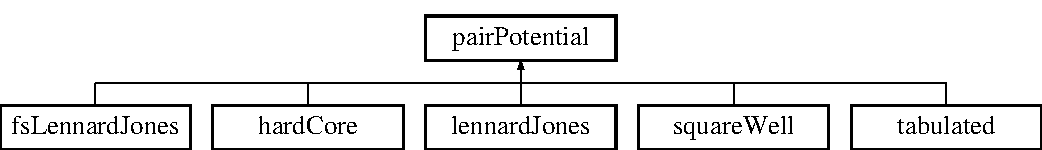
\includegraphics[height=2.000000cm]{classpair_potential}
\end{center}
\end{figure}
\subsection*{Public Member Functions}
\begin{DoxyCompactItemize}
\item 
\hyperlink{classpair_potential_a97a5ee64f179cbc0636dc2364fe7f7f4}{pair\+Potential} ()
\item 
virtual \hyperlink{classpair_potential_a8b68006b0fa57cb78c31e6dd2a8dde86}{$\sim$pair\+Potential} ()
\item 
virtual double \hyperlink{classpair_potential_a43dc9c840e25dc76e76d6ad7947c165d}{energy} (const double r)=0
\item 
virtual double \hyperlink{classpair_potential_a5387d21d8d487d1d42e9eaf7cae9175b}{tail\+Correction} (const double rho\+Bath)=0
\item 
virtual void \hyperlink{classpair_potential_ad4b237646f9de2ae9f95cc9350564bc5}{set\+Parameters} (const std\+::vector$<$ double $>$ params)=0
\item 
virtual double \hyperlink{classpair_potential_abf4f8d231c5e2e36d72916d33dcd75f0}{rcut} ()=0
\begin{DoxyCompactList}\small\item\em All potentials should be able to return their r\+\_\+\{cut\} values so neighbor lists, etc. \end{DoxyCompactList}\item 
double \hyperlink{classpair_potential_a1163a4943615f1c3e82b0630aedcba18}{energy} (const std\+::vector$<$ double $>$ \&p1, const std\+::vector$<$ double $>$ \&p2, const std\+::vector$<$ double $>$ \&box)
\begin{DoxyCompactList}\small\item\em Calculates the minimum image distance and invokes the energy call. \end{DoxyCompactList}\item 
void \hyperlink{classpair_potential_a2d57e0c3678ef3624cc1edc2a4f5d121}{save\+Potential} (std\+::string filename, double start, double dr)
\begin{DoxyCompactList}\small\item\em Function for saving arbitrary potential into A\+S\+C\+I\+I file. \end{DoxyCompactList}\end{DoxyCompactItemize}
\subsection*{Public Attributes}
\begin{DoxyCompactItemize}
\item 
bool \hyperlink{classpair_potential_ab4b4538a7e13771f50a29aaac2443037}{use\+Tail\+Correction}
\item 
std\+::vector$<$ double $>$ \hyperlink{classpair_potential_abf8ec8af983d6e9960bd149da099e883}{params\+\_\+}
\begin{DoxyCompactList}\small\item\em Parameters (constants) that are needed to calculate U(r) \end{DoxyCompactList}\item 
bool \hyperlink{classpair_potential_a635755c0a952bfc05a4cfae230c3dbd2}{params\+Are\+Set\+\_\+}
\begin{DoxyCompactList}\small\item\em Logical check if the paramters for this potential have been specified by the user. \end{DoxyCompactList}\end{DoxyCompactItemize}


\subsection{Detailed Description}
Abstract base class which defines all pair potentials. 

Definition at line 15 of file potentials.\+h.



\subsection{Constructor \& Destructor Documentation}
\hypertarget{classpair_potential_a97a5ee64f179cbc0636dc2364fe7f7f4}{}\index{pair\+Potential@{pair\+Potential}!pair\+Potential@{pair\+Potential}}
\index{pair\+Potential@{pair\+Potential}!pair\+Potential@{pair\+Potential}}
\subsubsection[{pair\+Potential()}]{\setlength{\rightskip}{0pt plus 5cm}pair\+Potential\+::pair\+Potential (
\begin{DoxyParamCaption}
{}
\end{DoxyParamCaption}
)\hspace{0.3cm}{\ttfamily [inline]}}\label{classpair_potential_a97a5ee64f179cbc0636dc2364fe7f7f4}


Definition at line 17 of file potentials.\+h.



References params\+Are\+Set\+\_\+.


\begin{DoxyCode}
17 \{ \hyperlink{classpair_potential_a635755c0a952bfc05a4cfae230c3dbd2}{paramsAreSet\_} = \textcolor{keyword}{false}; \}
\end{DoxyCode}
\hypertarget{classpair_potential_a8b68006b0fa57cb78c31e6dd2a8dde86}{}\index{pair\+Potential@{pair\+Potential}!````~pair\+Potential@{$\sim$pair\+Potential}}
\index{````~pair\+Potential@{$\sim$pair\+Potential}!pair\+Potential@{pair\+Potential}}
\subsubsection[{$\sim$pair\+Potential()}]{\setlength{\rightskip}{0pt plus 5cm}virtual pair\+Potential\+::$\sim$pair\+Potential (
\begin{DoxyParamCaption}
{}
\end{DoxyParamCaption}
)\hspace{0.3cm}{\ttfamily [inline]}, {\ttfamily [virtual]}}\label{classpair_potential_a8b68006b0fa57cb78c31e6dd2a8dde86}


Definition at line 18 of file potentials.\+h.


\begin{DoxyCode}
18 \{;\}
\end{DoxyCode}


\subsection{Member Function Documentation}
\hypertarget{classpair_potential_a43dc9c840e25dc76e76d6ad7947c165d}{}\index{pair\+Potential@{pair\+Potential}!energy@{energy}}
\index{energy@{energy}!pair\+Potential@{pair\+Potential}}
\subsubsection[{energy(const double r)=0}]{\setlength{\rightskip}{0pt plus 5cm}virtual double pair\+Potential\+::energy (
\begin{DoxyParamCaption}
\item[{const double}]{r}
\end{DoxyParamCaption}
)\hspace{0.3cm}{\ttfamily [pure virtual]}}\label{classpair_potential_a43dc9c840e25dc76e76d6ad7947c165d}


Implemented in \hyperlink{classhard_core_a5be8073d4b94045473352c9b56af69e5}{hard\+Core}, \hyperlink{classsquare_well_a318e7456943ad7c7f36cce0c9e2b2688}{square\+Well}, \hyperlink{classtabulated_a09fdfccca3e19adb68da74f0baac7423}{tabulated}, and \hyperlink{classlennard_jones_af90284faab4a29b15099794c25333a64}{lennard\+Jones}.



Referenced by save\+Potential().

\hypertarget{classpair_potential_a1163a4943615f1c3e82b0630aedcba18}{}\index{pair\+Potential@{pair\+Potential}!energy@{energy}}
\index{energy@{energy}!pair\+Potential@{pair\+Potential}}
\subsubsection[{energy(const std\+::vector$<$ double $>$ \&p1, const std\+::vector$<$ double $>$ \&p2, const std\+::vector$<$ double $>$ \&box)}]{\setlength{\rightskip}{0pt plus 5cm}double pair\+Potential\+::energy (
\begin{DoxyParamCaption}
\item[{const std\+::vector$<$ double $>$ \&}]{p1, }
\item[{const std\+::vector$<$ double $>$ \&}]{p2, }
\item[{const std\+::vector$<$ double $>$ \&}]{box}
\end{DoxyParamCaption}
)\hspace{0.3cm}{\ttfamily [inline]}}\label{classpair_potential_a1163a4943615f1c3e82b0630aedcba18}


Calculates the minimum image distance and invokes the energy call. 



Definition at line 26 of file potentials.\+h.



References energy(), and pbc\+\_\+dist2().



Referenced by energy().

\hypertarget{classpair_potential_abf4f8d231c5e2e36d72916d33dcd75f0}{}\index{pair\+Potential@{pair\+Potential}!rcut@{rcut}}
\index{rcut@{rcut}!pair\+Potential@{pair\+Potential}}
\subsubsection[{rcut()=0}]{\setlength{\rightskip}{0pt plus 5cm}virtual double pair\+Potential\+::rcut (
\begin{DoxyParamCaption}
{}
\end{DoxyParamCaption}
)\hspace{0.3cm}{\ttfamily [pure virtual]}}\label{classpair_potential_abf4f8d231c5e2e36d72916d33dcd75f0}


All potentials should be able to return their r\+\_\+\{cut\} values so neighbor lists, etc. 

can use them 

Implemented in \hyperlink{classhard_core_a3cbf5ecde18b2f2798a4b1aba1801ca5}{hard\+Core}, \hyperlink{classsquare_well_a82e1cc1009bd8e42e79e3c5f856f1b3b}{square\+Well}, \hyperlink{classtabulated_a1826f920afd53d74e17c8fa5253a2d2b}{tabulated}, and \hyperlink{classlennard_jones_a6ab5b04c385544da0de985e9635a6e8c}{lennard\+Jones}.



Referenced by sim\+System\+::add\+Potential(), and save\+Potential().

\hypertarget{classpair_potential_a2d57e0c3678ef3624cc1edc2a4f5d121}{}\index{pair\+Potential@{pair\+Potential}!save\+Potential@{save\+Potential}}
\index{save\+Potential@{save\+Potential}!pair\+Potential@{pair\+Potential}}
\subsubsection[{save\+Potential(std\+::string filename, double start, double dr)}]{\setlength{\rightskip}{0pt plus 5cm}void pair\+Potential\+::save\+Potential (
\begin{DoxyParamCaption}
\item[{std\+::string}]{filename, }
\item[{double}]{start, }
\item[{double}]{dr}
\end{DoxyParamCaption}
)}\label{classpair_potential_a2d57e0c3678ef3624cc1edc2a4f5d121}


Function for saving arbitrary potential into A\+S\+C\+I\+I file. 


\begin{DoxyParams}[1]{Parameters}
\mbox{\tt in}  & {\em filename} & Name of A\+S\+C\+I\+I file to save potential to \\
\hline
\mbox{\tt in}  & {\em start} & r value to start printing U(r) from \\
\hline
\mbox{\tt in}  & {\em dr} & Increment to move in r between prints \\
\hline
\end{DoxyParams}


Definition at line 10 of file potentials.\+cpp.



References energy(), and rcut().


\begin{DoxyCode}
11 \{
12                 \textcolor{keywordflow}{if} (dr <= 0.0) \{
13                                 \textcolor{keywordflow}{throw} \hyperlink{classcustom_exception}{customException}(\textcolor{stringliteral}{"The value for dr must be positive"});
14                 \}
15                 
16                 \textcolor{keywordtype}{double} r = start;
17                 std::ofstream outData(filename.c\_str());
18                                 
19                 \textcolor{keywordflow}{while} (r < \hyperlink{classpair_potential_abf4f8d231c5e2e36d72916d33dcd75f0}{rcut}()) \{
20                                 outData<<r<<\textcolor{stringliteral}{"\(\backslash\)t"}<<\hyperlink{classpair_potential_a43dc9c840e25dc76e76d6ad7947c165d}{energy}(r)<<std::endl;                   
21                                 r += dr;
22                 \}
23                 
24                 outData.close();
25 \}
\end{DoxyCode}
\hypertarget{classpair_potential_ad4b237646f9de2ae9f95cc9350564bc5}{}\index{pair\+Potential@{pair\+Potential}!set\+Parameters@{set\+Parameters}}
\index{set\+Parameters@{set\+Parameters}!pair\+Potential@{pair\+Potential}}
\subsubsection[{set\+Parameters(const std\+::vector$<$ double $>$ params)=0}]{\setlength{\rightskip}{0pt plus 5cm}virtual void pair\+Potential\+::set\+Parameters (
\begin{DoxyParamCaption}
\item[{const std\+::vector$<$ double $>$}]{params}
\end{DoxyParamCaption}
)\hspace{0.3cm}{\ttfamily [pure virtual]}}\label{classpair_potential_ad4b237646f9de2ae9f95cc9350564bc5}


Implemented in \hyperlink{classhard_core_a2bbf6a77445f5cb5fc1a3c37ba0e6566}{hard\+Core}, \hyperlink{classsquare_well_aa8770429044914778c2f343e025e09cc}{square\+Well}, \hyperlink{classtabulated_a6a52e8a5b99ddd16fcbd3e404c90f559}{tabulated}, and \hyperlink{classlennard_jones_a5b4c41df05048ce99bffb9f27733100a}{lennard\+Jones}.

\hypertarget{classpair_potential_a5387d21d8d487d1d42e9eaf7cae9175b}{}\index{pair\+Potential@{pair\+Potential}!tail\+Correction@{tail\+Correction}}
\index{tail\+Correction@{tail\+Correction}!pair\+Potential@{pair\+Potential}}
\subsubsection[{tail\+Correction(const double rho\+Bath)=0}]{\setlength{\rightskip}{0pt plus 5cm}virtual double pair\+Potential\+::tail\+Correction (
\begin{DoxyParamCaption}
\item[{const double}]{rho\+Bath}
\end{DoxyParamCaption}
)\hspace{0.3cm}{\ttfamily [pure virtual]}}\label{classpair_potential_a5387d21d8d487d1d42e9eaf7cae9175b}


Implemented in \hyperlink{classhard_core_a90c73dbda39a9c48f1f26474474183e4}{hard\+Core}, \hyperlink{classsquare_well_a3a81297ea3a06f8a354c824a7ac5dc94}{square\+Well}, \hyperlink{classtabulated_afb2936dfc0ba4255eb06f9d81e594dd2}{tabulated}, and \hyperlink{classlennard_jones_a4518a7a9970c1fbed2f2abcf0ceebbfc}{lennard\+Jones}.



\subsection{Member Data Documentation}
\hypertarget{classpair_potential_abf8ec8af983d6e9960bd149da099e883}{}\index{pair\+Potential@{pair\+Potential}!params\+\_\+@{params\+\_\+}}
\index{params\+\_\+@{params\+\_\+}!pair\+Potential@{pair\+Potential}}
\subsubsection[{params\+\_\+}]{\setlength{\rightskip}{0pt plus 5cm}std\+::vector$<$ double $>$ pair\+Potential\+::params\+\_\+}\label{classpair_potential_abf8ec8af983d6e9960bd149da099e883}


Parameters (constants) that are needed to calculate U(r) 



Definition at line 29 of file potentials.\+h.



Referenced by lennard\+Jones\+::energy(), tabulated\+::energy(), square\+Well\+::energy(), hard\+Core\+::energy(), tabulated\+::load\+Potential(), lennard\+Jones\+::rcut(), tabulated\+::rcut(), square\+Well\+::rcut(), hard\+Core\+::rcut(), lennard\+Jones\+::set\+Parameters(), tabulated\+::set\+Parameters(), square\+Well\+::set\+Parameters(), hard\+Core\+::set\+Parameters(), and lennard\+Jones\+::tail\+Correction().

\hypertarget{classpair_potential_a635755c0a952bfc05a4cfae230c3dbd2}{}\index{pair\+Potential@{pair\+Potential}!params\+Are\+Set\+\_\+@{params\+Are\+Set\+\_\+}}
\index{params\+Are\+Set\+\_\+@{params\+Are\+Set\+\_\+}!pair\+Potential@{pair\+Potential}}
\subsubsection[{params\+Are\+Set\+\_\+}]{\setlength{\rightskip}{0pt plus 5cm}bool pair\+Potential\+::params\+Are\+Set\+\_\+}\label{classpair_potential_a635755c0a952bfc05a4cfae230c3dbd2}


Logical check if the paramters for this potential have been specified by the user. 



Definition at line 30 of file potentials.\+h.



Referenced by lennard\+Jones\+::energy(), tabulated\+::energy(), square\+Well\+::energy(), hard\+Core\+::energy(), tabulated\+::load\+Potential(), pair\+Potential(), lennard\+Jones\+::rcut(), tabulated\+::rcut(), square\+Well\+::rcut(), hard\+Core\+::rcut(), lennard\+Jones\+::set\+Parameters(), tabulated\+::set\+Parameters(), square\+Well\+::set\+Parameters(), and hard\+Core\+::set\+Parameters().

\hypertarget{classpair_potential_ab4b4538a7e13771f50a29aaac2443037}{}\index{pair\+Potential@{pair\+Potential}!use\+Tail\+Correction@{use\+Tail\+Correction}}
\index{use\+Tail\+Correction@{use\+Tail\+Correction}!pair\+Potential@{pair\+Potential}}
\subsubsection[{use\+Tail\+Correction}]{\setlength{\rightskip}{0pt plus 5cm}bool pair\+Potential\+::use\+Tail\+Correction}\label{classpair_potential_ab4b4538a7e13771f50a29aaac2443037}


Definition at line 20 of file potentials.\+h.



Referenced by lennard\+Jones\+::set\+Parameters(), tabulated\+::set\+Parameters(), square\+Well\+::set\+Parameters(), and hard\+Core\+::set\+Parameters().



The documentation for this class was generated from the following files\+:\begin{DoxyCompactItemize}
\item 
/\+Users/nam4/\+Desktop/omcs/src/\hyperlink{potentials_8h}{potentials.\+h}\item 
/\+Users/nam4/\+Desktop/omcs/src/\hyperlink{potentials_8cpp}{potentials.\+cpp}\end{DoxyCompactItemize}

\hypertarget{classquaternion}{\section{quaternion Class Reference}
\label{classquaternion}\index{quaternion@{quaternion}}
}


{\ttfamily \#include $<$quaternion.\-h$>$}

\subsection*{Public Member Functions}
\begin{DoxyCompactItemize}
\item 
\hyperlink{classquaternion_a66be1b74fcbd7d2bf8b92d0ff3760c03}{quaternion} ()
\item 
\hyperlink{classquaternion_afde1d3e0610d4e72a544ef8b329f0588}{$\sim$quaternion} ()
\item 
void \hyperlink{classquaternion_ad3b1869658470d5adae436fe6f98e1f0}{set} (const std\-::vector$<$ double $>$ \&q)
\begin{DoxyCompactList}\small\item\em Set the quaternion's value. \end{DoxyCompactList}\item 
void \hyperlink{classquaternion_a05a1549d902c5cd6401985caaf1a7e3f}{set\-Axis\-Angle} (const std\-::vector$<$ double $>$ \&u, const double angle)
\begin{DoxyCompactList}\small\item\em Set the quaternion based on angle, axis desired. \end{DoxyCompactList}\item 
void \hyperlink{classquaternion_a370e464ed34ec78540481a35b9a6829e}{set\-Random\-Rot} ()
\begin{DoxyCompactList}\small\item\em Pick a quaternion that corresponds to a random 3\-D rotation. \end{DoxyCompactList}\item 
void \hyperlink{classquaternion_a5500ac17c80600120b5036fee3796052}{conjugate} ()
\begin{DoxyCompactList}\small\item\em Transform quaternion into its conjugate. \end{DoxyCompactList}\item 
void \hyperlink{classquaternion_a056b14ed0f5b2ab02667aeedb58d1725}{normalize} ()
\begin{DoxyCompactList}\small\item\em Normalize a quaternion. \end{DoxyCompactList}\item 
void \hyperlink{classquaternion_a1fa2dac4be850e01aa08103dac746b64}{inverse} ()
\begin{DoxyCompactList}\small\item\em Transform a quanternion into its inverse. \end{DoxyCompactList}\item 
void \hyperlink{classquaternion_ab8f466daaaa9a122a86da6fe713f62fe}{translate} (const std\-::vector$<$ double $>$ \&t)
\begin{DoxyCompactList}\small\item\em Translate a quaternion in 3\-D space. \end{DoxyCompactList}\item 
double \hyperlink{classquaternion_a28ff31359622e09c9c292f78cf08b801}{get\-Norm} ()
\begin{DoxyCompactList}\small\item\em Return the norm of the quaternion. \end{DoxyCompactList}\item 
std\-::vector$<$ double $>$ \hyperlink{classquaternion_af701c4a67c60f98af80e3c3caeb5bd4a}{get} ()
\item 
std\-::vector$<$ double $>$ \hyperlink{classquaternion_a618cce42beeb9ab3c724c4a9e6f37f55}{rotate\-Vec} (const std\-::vector$<$ double $>$ \&vec)
\begin{DoxyCompactList}\small\item\em Use this quaternion to operate on a vector, that causes its rotation. \end{DoxyCompactList}\item 
\hyperlink{classquaternion}{quaternion} \hyperlink{classquaternion_a3cf72d92681c00362e59e7ff96d0ea4f}{operator+} (const \hyperlink{classquaternion}{quaternion} \&p)
\begin{DoxyCompactList}\small\item\em Add a quaternion to this one. \end{DoxyCompactList}\item 
\hyperlink{classquaternion}{quaternion} \hyperlink{classquaternion_af299a0ea61d45ff4cb9a8551e7cad01a}{operator-\/} (const \hyperlink{classquaternion}{quaternion} \&p)
\begin{DoxyCompactList}\small\item\em Subtract a quaternion from this one. \end{DoxyCompactList}\item 
\hyperlink{classquaternion}{quaternion} \hyperlink{classquaternion_ab8c2b2a742c75b683f75f763a8ecf0aa}{operator$\ast$} (const \hyperlink{classquaternion}{quaternion} \&other)
\begin{DoxyCompactList}\small\item\em Multiply this quaternion by another. \end{DoxyCompactList}\item 
bool \hyperlink{classquaternion_ae7b568fc0cc23d9248ae38ec944865ff}{operator==} (const \hyperlink{classquaternion}{quaternion} \&other)
\begin{DoxyCompactList}\small\item\em Check if two quaternions are equal to each other to within a tolerance of 1.\-0e-\/12. \end{DoxyCompactList}\item 
bool \hyperlink{classquaternion_a9ed9d3b39020b800e55033efd1fe8e45}{operator!=} (const \hyperlink{classquaternion}{quaternion} \&other)
\begin{DoxyCompactList}\small\item\em Check if two quaternions are not equal to each other to within a tolerance of 1.\-0e-\/12. \end{DoxyCompactList}\end{DoxyCompactItemize}


\subsection{Detailed Description}


Definition at line 9 of file quaternion.\-h.



\subsection{Constructor \& Destructor Documentation}
\hypertarget{classquaternion_a66be1b74fcbd7d2bf8b92d0ff3760c03}{\index{quaternion@{quaternion}!quaternion@{quaternion}}
\index{quaternion@{quaternion}!quaternion@{quaternion}}
\subsubsection[{quaternion}]{\setlength{\rightskip}{0pt plus 5cm}quaternion\-::quaternion (
\begin{DoxyParamCaption}
{}
\end{DoxyParamCaption}
)\hspace{0.3cm}{\ttfamily [inline]}}}\label{classquaternion_a66be1b74fcbd7d2bf8b92d0ff3760c03}


Definition at line 11 of file quaternion.\-h.



References set\-Random\-Rot().


\begin{DoxyCode}
11 \{ q\_.resize(4, 0.0); std::vector < double > dummy (3, 0); R\_.resize(3, dummy); 
      \hyperlink{classquaternion_a370e464ed34ec78540481a35b9a6829e}{setRandomRot} (); \}
\end{DoxyCode}
\hypertarget{classquaternion_afde1d3e0610d4e72a544ef8b329f0588}{\index{quaternion@{quaternion}!$\sim$quaternion@{$\sim$quaternion}}
\index{$\sim$quaternion@{$\sim$quaternion}!quaternion@{quaternion}}
\subsubsection[{$\sim$quaternion}]{\setlength{\rightskip}{0pt plus 5cm}quaternion\-::$\sim$quaternion (
\begin{DoxyParamCaption}
{}
\end{DoxyParamCaption}
)\hspace{0.3cm}{\ttfamily [inline]}}}\label{classquaternion_afde1d3e0610d4e72a544ef8b329f0588}


Definition at line 12 of file quaternion.\-h.


\begin{DoxyCode}
12 \{\};
\end{DoxyCode}


\subsection{Member Function Documentation}
\hypertarget{classquaternion_a5500ac17c80600120b5036fee3796052}{\index{quaternion@{quaternion}!conjugate@{conjugate}}
\index{conjugate@{conjugate}!quaternion@{quaternion}}
\subsubsection[{conjugate}]{\setlength{\rightskip}{0pt plus 5cm}void quaternion\-::conjugate (
\begin{DoxyParamCaption}
{}
\end{DoxyParamCaption}
)}}\label{classquaternion_a5500ac17c80600120b5036fee3796052}


Transform quaternion into its conjugate. 



Definition at line 53 of file quaternion.\-cpp.



Referenced by inverse().


\begin{DoxyCode}
53                             \{
54     \textcolor{keywordflow}{for} (\textcolor{keywordtype}{unsigned} \textcolor{keywordtype}{int} i = 1; i < 4; ++i) \{
55         q\_[i] = -q\_[i];
56     \}
57 \}
\end{DoxyCode}
\hypertarget{classquaternion_af701c4a67c60f98af80e3c3caeb5bd4a}{\index{quaternion@{quaternion}!get@{get}}
\index{get@{get}!quaternion@{quaternion}}
\subsubsection[{get}]{\setlength{\rightskip}{0pt plus 5cm}std\-::vector$<$ double $>$ quaternion\-::get (
\begin{DoxyParamCaption}
{}
\end{DoxyParamCaption}
)\hspace{0.3cm}{\ttfamily [inline]}}}\label{classquaternion_af701c4a67c60f98af80e3c3caeb5bd4a}


Definition at line 24 of file quaternion.\-h.


\begin{DoxyCode}
24 \{ \textcolor{keywordflow}{return} q\_; \} \textcolor{comment}{// Return the quaternion's values}
\end{DoxyCode}
\hypertarget{classquaternion_a28ff31359622e09c9c292f78cf08b801}{\index{quaternion@{quaternion}!get\-Norm@{get\-Norm}}
\index{get\-Norm@{get\-Norm}!quaternion@{quaternion}}
\subsubsection[{get\-Norm}]{\setlength{\rightskip}{0pt plus 5cm}double quaternion\-::get\-Norm (
\begin{DoxyParamCaption}
{}
\end{DoxyParamCaption}
)}}\label{classquaternion_a28ff31359622e09c9c292f78cf08b801}


Return the norm of the quaternion. 



Definition at line 102 of file quaternion.\-cpp.



Referenced by normalize().


\begin{DoxyCode}
102                             \{
103     \textcolor{keywordtype}{double} n2 = 0.0;
104     \textcolor{keywordflow}{for} (\textcolor{keywordtype}{unsigned} \textcolor{keywordtype}{int} i = 0; i < 4; ++i) \{
105         n2 += q\_[i]*q\_[i];
106     \}
107     \textcolor{keywordflow}{return} std::sqrt(n2);
108 \}
\end{DoxyCode}
\hypertarget{classquaternion_a1fa2dac4be850e01aa08103dac746b64}{\index{quaternion@{quaternion}!inverse@{inverse}}
\index{inverse@{inverse}!quaternion@{quaternion}}
\subsubsection[{inverse}]{\setlength{\rightskip}{0pt plus 5cm}void quaternion\-::inverse (
\begin{DoxyParamCaption}
{}
\end{DoxyParamCaption}
)}}\label{classquaternion_a1fa2dac4be850e01aa08103dac746b64}


Transform a quanternion into its inverse. 



Definition at line 74 of file quaternion.\-cpp.



References conjugate().


\begin{DoxyCode}
74                           \{
75     \hyperlink{classquaternion_a5500ac17c80600120b5036fee3796052}{conjugate}();
76     \textcolor{keywordtype}{double} n2 = 0.0;
77     \textcolor{keywordflow}{for} (\textcolor{keywordtype}{unsigned} \textcolor{keywordtype}{int} i = 0; i < 4; ++i) \{
78         n2 += q\_[i]*q\_[i];
79     \}
80     \textcolor{keywordflow}{for} (\textcolor{keywordtype}{unsigned} \textcolor{keywordtype}{int} i = 0; i < 4; ++i) \{
81         q\_[i] /= n2;
82     \}
83 \}
\end{DoxyCode}
\hypertarget{classquaternion_a056b14ed0f5b2ab02667aeedb58d1725}{\index{quaternion@{quaternion}!normalize@{normalize}}
\index{normalize@{normalize}!quaternion@{quaternion}}
\subsubsection[{normalize}]{\setlength{\rightskip}{0pt plus 5cm}void quaternion\-::normalize (
\begin{DoxyParamCaption}
{}
\end{DoxyParamCaption}
)}}\label{classquaternion_a056b14ed0f5b2ab02667aeedb58d1725}


Normalize a quaternion. 


\begin{DoxyParams}[1]{Parameters}
\mbox{\tt in}  & {\em t} & Translation vector. \\
\hline
\end{DoxyParams}


Definition at line 64 of file quaternion.\-cpp.



References get\-Norm().


\begin{DoxyCode}
64                             \{
65     \textcolor{keyword}{const} \textcolor{keywordtype}{double} norm = \hyperlink{classquaternion_a28ff31359622e09c9c292f78cf08b801}{getNorm}();
66     \textcolor{keywordflow}{for} (\textcolor{keywordtype}{unsigned} \textcolor{keywordtype}{int} i = 0; i < 4; ++i) \{
67         q\_[i] /= norm;
68     \}
69 \}
\end{DoxyCode}
\hypertarget{classquaternion_a9ed9d3b39020b800e55033efd1fe8e45}{\index{quaternion@{quaternion}!operator!=@{operator!=}}
\index{operator!=@{operator!=}!quaternion@{quaternion}}
\subsubsection[{operator!=}]{\setlength{\rightskip}{0pt plus 5cm}bool quaternion\-::operator!= (
\begin{DoxyParamCaption}
\item[{const {\bf quaternion} \&}]{other}
\end{DoxyParamCaption}
)\hspace{0.3cm}{\ttfamily [inline]}}}\label{classquaternion_a9ed9d3b39020b800e55033efd1fe8e45}


Check if two quaternions are not equal to each other to within a tolerance of 1.\-0e-\/12. 


\begin{DoxyParams}[1]{Parameters}
\mbox{\tt in}  & {\em other} & Other quaternion to compare with. \\
\hline
\end{DoxyParams}


Definition at line 94 of file quaternion.\-h.


\begin{DoxyCode}
94                                               \{
95         \textcolor{keywordflow}{return} !(*\textcolor{keyword}{this} == other);
96     \}
\end{DoxyCode}
\hypertarget{classquaternion_ab8c2b2a742c75b683f75f763a8ecf0aa}{\index{quaternion@{quaternion}!operator$\ast$@{operator$\ast$}}
\index{operator$\ast$@{operator$\ast$}!quaternion@{quaternion}}
\subsubsection[{operator$\ast$}]{\setlength{\rightskip}{0pt plus 5cm}{\bf quaternion} quaternion\-::operator$\ast$ (
\begin{DoxyParamCaption}
\item[{const {\bf quaternion} \&}]{other}
\end{DoxyParamCaption}
)\hspace{0.3cm}{\ttfamily [inline]}}}\label{classquaternion_ab8c2b2a742c75b683f75f763a8ecf0aa}


Multiply this quaternion by another. 

Does this in order of self$\ast$other.


\begin{DoxyParams}[1]{Parameters}
\mbox{\tt in}  & {\em other} & Quaternion to multiply this one by.\\
\hline
\end{DoxyParams}
\begin{DoxyReturn}{Returns}
self$\ast$other 
\end{DoxyReturn}


Definition at line 64 of file quaternion.\-h.



References set().


\begin{DoxyCode}
64                                                    \{
65         \hyperlink{classquaternion}{quaternion} ans;
66         std::vector < double > prod (4, 0);
67         prod[0] = this->q\_[0]*other.q\_[0] - this->q\_[1]*other.q\_[1] - this->q\_[2]*other.q\_[2] - this->q\_[3]
      *other.q\_[3];
68         prod[1] = this->q\_[0]*other.q\_[1] + this->q\_[1]*other.q\_[0] + this->q\_[2]*other.q\_[3] - this->q\_[3]
      *other.q\_[2];
69         prod[2] = this->q\_[0]*other.q\_[2] - this->q\_[1]*other.q\_[3] + this->q\_[2]*other.q\_[0] + this->q\_[3]
      *other.q\_[1];
70         prod[3] = this->q\_[0]*other.q\_[3] + this->q\_[1]*other.q\_[2] - this->q\_[2]*other.q\_[1] + this->q\_[3]
      *other.q\_[0];
71         ans.\hyperlink{classquaternion_ad3b1869658470d5adae436fe6f98e1f0}{set}(prod);
72         \textcolor{keywordflow}{return} ans;
73     \}
\end{DoxyCode}
\hypertarget{classquaternion_a3cf72d92681c00362e59e7ff96d0ea4f}{\index{quaternion@{quaternion}!operator+@{operator+}}
\index{operator+@{operator+}!quaternion@{quaternion}}
\subsubsection[{operator+}]{\setlength{\rightskip}{0pt plus 5cm}{\bf quaternion} quaternion\-::operator+ (
\begin{DoxyParamCaption}
\item[{const {\bf quaternion} \&}]{p}
\end{DoxyParamCaption}
)\hspace{0.3cm}{\ttfamily [inline]}}}\label{classquaternion_a3cf72d92681c00362e59e7ff96d0ea4f}


Add a quaternion to this one. 


\begin{DoxyParams}[1]{Parameters}
\mbox{\tt in}  & {\em p} & Quaternion to add to this one. \\
\hline
\end{DoxyParams}


Definition at line 32 of file quaternion.\-h.



References set().


\begin{DoxyCode}
32                                                \{
33         \hyperlink{classquaternion}{quaternion} ans;
34         std::vector < double > sum (4, 0);
35         \textcolor{keywordflow}{for} (\textcolor{keywordtype}{unsigned} \textcolor{keywordtype}{int} i = 0; i < 4; ++i) \{
36             sum[i] = this->q\_[i] + p.q\_[i];
37         \}
38         ans.\hyperlink{classquaternion_ad3b1869658470d5adae436fe6f98e1f0}{set}(sum);
39         \textcolor{keywordflow}{return} ans;
40     \}
\end{DoxyCode}
\hypertarget{classquaternion_af299a0ea61d45ff4cb9a8551e7cad01a}{\index{quaternion@{quaternion}!operator-\/@{operator-\/}}
\index{operator-\/@{operator-\/}!quaternion@{quaternion}}
\subsubsection[{operator-\/}]{\setlength{\rightskip}{0pt plus 5cm}{\bf quaternion} quaternion\-::operator-\/ (
\begin{DoxyParamCaption}
\item[{const {\bf quaternion} \&}]{p}
\end{DoxyParamCaption}
)\hspace{0.3cm}{\ttfamily [inline]}}}\label{classquaternion_af299a0ea61d45ff4cb9a8551e7cad01a}


Subtract a quaternion from this one. 


\begin{DoxyParams}[1]{Parameters}
\mbox{\tt in}  & {\em p} & Quaternion to subtract from this one. \\
\hline
\end{DoxyParams}


Definition at line 47 of file quaternion.\-h.



References set().


\begin{DoxyCode}
47                                                \{
48         \hyperlink{classquaternion}{quaternion} ans;
49         std::vector < double > sum (4, 0);
50         \textcolor{keywordflow}{for} (\textcolor{keywordtype}{unsigned} \textcolor{keywordtype}{int} i = 0; i < 4; ++i) \{
51             sum[i] = this->q\_[i] - p.q\_[i];
52         \}
53         ans.\hyperlink{classquaternion_ad3b1869658470d5adae436fe6f98e1f0}{set}(sum);
54         \textcolor{keywordflow}{return} ans;
55     \}
\end{DoxyCode}
\hypertarget{classquaternion_ae7b568fc0cc23d9248ae38ec944865ff}{\index{quaternion@{quaternion}!operator==@{operator==}}
\index{operator==@{operator==}!quaternion@{quaternion}}
\subsubsection[{operator==}]{\setlength{\rightskip}{0pt plus 5cm}bool quaternion\-::operator== (
\begin{DoxyParamCaption}
\item[{const {\bf quaternion} \&}]{other}
\end{DoxyParamCaption}
)\hspace{0.3cm}{\ttfamily [inline]}}}\label{classquaternion_ae7b568fc0cc23d9248ae38ec944865ff}


Check if two quaternions are equal to each other to within a tolerance of 1.\-0e-\/12. 


\begin{DoxyParams}[1]{Parameters}
\mbox{\tt in}  & {\em other} & Other quaternion to compare with. \\
\hline
\end{DoxyParams}


Definition at line 80 of file quaternion.\-h.


\begin{DoxyCode}
80                                               \{
81         \textcolor{keywordflow}{for} (\textcolor{keywordtype}{unsigned} \textcolor{keywordtype}{int} i = 0; i < 4; ++i) \{
82             \textcolor{keywordflow}{if} (fabs(this->q\_[i] - other.q\_[i]) > 1.0e-12) \{
83                 \textcolor{keywordflow}{return} \textcolor{keyword}{false};
84             \}
85         \}
86         \textcolor{keywordflow}{return} \textcolor{keyword}{true};
87     \}
\end{DoxyCode}
\hypertarget{classquaternion_a618cce42beeb9ab3c724c4a9e6f37f55}{\index{quaternion@{quaternion}!rotate\-Vec@{rotate\-Vec}}
\index{rotate\-Vec@{rotate\-Vec}!quaternion@{quaternion}}
\subsubsection[{rotate\-Vec}]{\setlength{\rightskip}{0pt plus 5cm}std\-::vector$<$ double $>$ quaternion\-::rotate\-Vec (
\begin{DoxyParamCaption}
\item[{const std\-::vector$<$ double $>$ \&}]{vec}
\end{DoxyParamCaption}
)}}\label{classquaternion_a618cce42beeb9ab3c724c4a9e6f37f55}


Use this quaternion to operate on a vector, that causes its rotation. 


\begin{DoxyParams}[1]{Parameters}
\mbox{\tt in}  & {\em vec} & Vector to rotate. \\
\hline
\end{DoxyParams}


Definition at line 115 of file quaternion.\-cpp.


\begin{DoxyCode}
115                                                                            \{
116     std::vector < double > ans (3, 0);
117     assignr\_ (q\_);
118 
119     \textcolor{keywordflow}{for} (\textcolor{keywordtype}{unsigned} \textcolor{keywordtype}{int} i = 0; i < 3; ++i) \{
120         \textcolor{keywordflow}{for} (\textcolor{keywordtype}{unsigned} \textcolor{keywordtype}{int} j = 0; j < 3; ++j) \{
121             ans[i] += R\_[i][j]*vec[j];
122         \}
123     \}
124 
125     \textcolor{keywordflow}{return} ans;
126 \}
\end{DoxyCode}
\hypertarget{classquaternion_ad3b1869658470d5adae436fe6f98e1f0}{\index{quaternion@{quaternion}!set@{set}}
\index{set@{set}!quaternion@{quaternion}}
\subsubsection[{set}]{\setlength{\rightskip}{0pt plus 5cm}void quaternion\-::set (
\begin{DoxyParamCaption}
\item[{const std\-::vector$<$ double $>$ \&}]{qv}
\end{DoxyParamCaption}
)}}\label{classquaternion_ad3b1869658470d5adae436fe6f98e1f0}


Set the quaternion's value. 


\begin{DoxyParams}[1]{Parameters}
\mbox{\tt in}  & {\em qv} & 4 component vector, \mbox{[}x, x, y, z\mbox{]} \\
\hline
\end{DoxyParams}


Definition at line 8 of file quaternion.\-cpp.



Referenced by operator$\ast$(), operator+(), and operator-\/().


\begin{DoxyCode}
8                                                     \{
9     assignq\_ (qv);
10 \}
\end{DoxyCode}
\hypertarget{classquaternion_a05a1549d902c5cd6401985caaf1a7e3f}{\index{quaternion@{quaternion}!set\-Axis\-Angle@{set\-Axis\-Angle}}
\index{set\-Axis\-Angle@{set\-Axis\-Angle}!quaternion@{quaternion}}
\subsubsection[{set\-Axis\-Angle}]{\setlength{\rightskip}{0pt plus 5cm}void quaternion\-::set\-Axis\-Angle (
\begin{DoxyParamCaption}
\item[{const std\-::vector$<$ double $>$ \&}]{u, }
\item[{const double}]{angle}
\end{DoxyParamCaption}
)}}\label{classquaternion_a05a1549d902c5cd6401985caaf1a7e3f}


Set the quaternion based on angle, axis desired. 

Does not need to be normalized.


\begin{DoxyParams}[1]{Parameters}
\mbox{\tt in}  & {\em angle} & Angle of rotation desired relative to axis (in radians) \\
\hline
\mbox{\tt in}  & {\em aixs} & 3\-D axis to rotate about (in right-\/handed coordinates) \\
\hline
\end{DoxyParams}


Definition at line 150 of file quaternion.\-cpp.


\begin{DoxyCode}
150                                                                                 \{
151     \textcolor{keywordflow}{if} (u.size() != 3) \{
152         \textcolor{keywordflow}{throw} \hyperlink{classcustom_exception}{customException} (\textcolor{stringliteral}{"Axis for Quaternion must have 3 elements"});
153     \}
154     q\_[0] = std::cos(angle/2.0);
155     \textcolor{keyword}{const} \textcolor{keywordtype}{double} s = std::sin(angle/2.0);
156     q\_[1] = s*u[0];
157     q\_[2] = s*u[1];
158     q\_[3] = s*u[2];
159 \}
\end{DoxyCode}
\hypertarget{classquaternion_a370e464ed34ec78540481a35b9a6829e}{\index{quaternion@{quaternion}!set\-Random\-Rot@{set\-Random\-Rot}}
\index{set\-Random\-Rot@{set\-Random\-Rot}!quaternion@{quaternion}}
\subsubsection[{set\-Random\-Rot}]{\setlength{\rightskip}{0pt plus 5cm}void quaternion\-::set\-Random\-Rot (
\begin{DoxyParamCaption}
{}
\end{DoxyParamCaption}
)}}\label{classquaternion_a370e464ed34ec78540481a35b9a6829e}


Pick a quaternion that corresponds to a random 3\-D rotation. 



Definition at line 131 of file quaternion.\-cpp.



References P\-I, rng(), and R\-N\-G\-\_\-\-S\-E\-E\-D.



Referenced by quaternion().


\begin{DoxyCode}
131                                 \{
132      \textcolor{comment}{// spherical coordinates to get random unit vector}
133      \textcolor{keyword}{const} \textcolor{keywordtype}{double} theta = std::acos(2.0*\hyperlink{utilities_8cpp_a0f9542af4b475ac79cb679d7a8d14db0}{rng}(&\hyperlink{global_8h_a3f4e4ea24d5a5c66feae55d1f329c884}{RNG\_SEED}) - 1.0);
134      \textcolor{keyword}{const} \textcolor{keywordtype}{double} phi = 2.0*\hyperlink{global_8h_a598a3330b3c21701223ee0ca14316eca}{PI}*\hyperlink{utilities_8cpp_a0f9542af4b475ac79cb679d7a8d14db0}{rng}(&\hyperlink{global_8h_a3f4e4ea24d5a5c66feae55d1f329c884}{RNG\_SEED}), sin\_phi = std::sin(phi);
135 
136      \textcolor{comment}{// randomly pick angle}
137      \textcolor{keyword}{const} \textcolor{keywordtype}{double} angle = 2.0*\hyperlink{global_8h_a598a3330b3c21701223ee0ca14316eca}{PI}*\hyperlink{utilities_8cpp_a0f9542af4b475ac79cb679d7a8d14db0}{rng}(&\hyperlink{global_8h_a3f4e4ea24d5a5c66feae55d1f329c884}{RNG\_SEED}), s = std::sin(angle/2.0);
138      q\_[0] = std::cos(angle/2.0);
139      q\_[1] = s*1.0*sin\_phi*std::cos(theta);
140      q\_[2] = s*1.0*sin\_phi*std::sin(theta);
141      q\_[3] = s*1.0*std::cos(phi);
142  \}
\end{DoxyCode}
\hypertarget{classquaternion_ab8f466daaaa9a122a86da6fe713f62fe}{\index{quaternion@{quaternion}!translate@{translate}}
\index{translate@{translate}!quaternion@{quaternion}}
\subsubsection[{translate}]{\setlength{\rightskip}{0pt plus 5cm}void quaternion\-::translate (
\begin{DoxyParamCaption}
\item[{const std\-::vector$<$ double $>$ \&}]{t}
\end{DoxyParamCaption}
)}}\label{classquaternion_ab8f466daaaa9a122a86da6fe713f62fe}


Translate a quaternion in 3\-D space. 


\begin{DoxyParams}[1]{Parameters}
\mbox{\tt in}  & {\em t} & Translation vector. \\
\hline
\end{DoxyParams}


Definition at line 90 of file quaternion.\-cpp.


\begin{DoxyCode}
90                                                          \{
91     \textcolor{keywordflow}{if} (t.size() != 3) \{
92         \textcolor{keywordflow}{throw} \hyperlink{classcustom_exception}{customException} (\textcolor{stringliteral}{"Translation vector for Quaternion must have 3 elements"});
93     \}
94     \textcolor{keywordflow}{for} (\textcolor{keywordtype}{unsigned} \textcolor{keywordtype}{int} i = 1; i < 4; ++i) \{
95         q\_[i] += t[i-1];
96     \}
97 \}
\end{DoxyCode}


The documentation for this class was generated from the following files\-:\begin{DoxyCompactItemize}
\item 
/home/nam4/\-Desktop/sandbox/\-F\-H\-M\-C\-Simulation/src/\hyperlink{quaternion_8h}{quaternion.\-h}\item 
/home/nam4/\-Desktop/sandbox/\-F\-H\-M\-C\-Simulation/src/\hyperlink{quaternion_8cpp}{quaternion.\-cpp}\end{DoxyCompactItemize}

\hypertarget{classright_triangle_x_z}{\section{right\-Triangle\-X\-Z Class Reference}
\label{classright_triangle_x_z}\index{right\-Triangle\-X\-Z@{right\-Triangle\-X\-Z}}
}


{\ttfamily \#include $<$barrier.\-h$>$}

Inheritance diagram for right\-Triangle\-X\-Z\-:\begin{figure}[H]
\begin{center}
\leavevmode
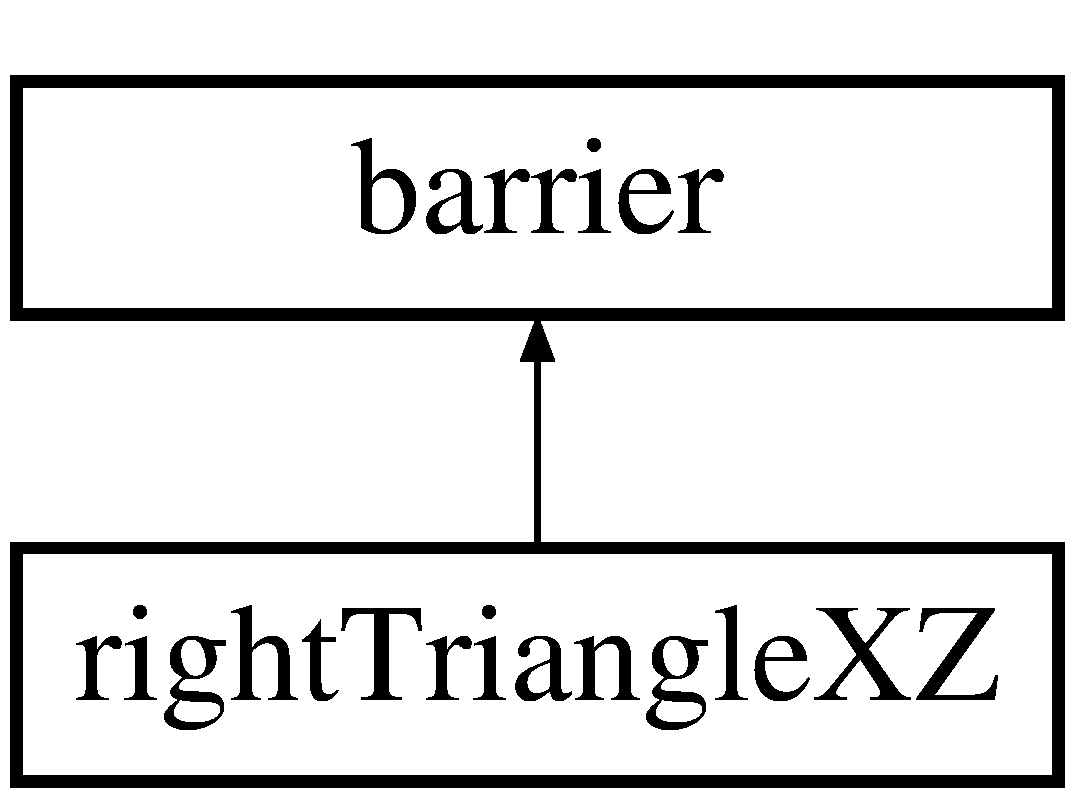
\includegraphics[height=2.000000cm]{classright_triangle_x_z}
\end{center}
\end{figure}
\subsection*{Public Member Functions}
\begin{DoxyCompactItemize}
\item 
\hyperlink{classright_triangle_x_z_a3ce16261ab80928bbfbc2b0d0aa67399}{$\sim$right\-Triangle\-X\-Z} ()
\item 
\hyperlink{classright_triangle_x_z_a8f252f8cb6cbe2861d05565484accc17}{right\-Triangle\-X\-Z} (const double width, const double theta, const double lam\-W, const double eps, const double sigma, const double sep, const double offset, const std\-::vector$<$ double $>$ \&box, const double zbase, bool top=false, const int M=1)
\begin{DoxyCompactList}\small\item\em Instantiate a right triangle feature with its base in the xy-\/plane. \end{DoxyCompactList}\item 
bool \hyperlink{classright_triangle_x_z_a574bcc38639a6d599aaa38fd9085ff63}{inside} (const \hyperlink{classatom}{atom} $\ast$a1, const std\-::vector$<$ double $>$ \&box)
\begin{DoxyCompactList}\small\item\em Check if an atom is overlapping the feature. \end{DoxyCompactList}\item 
double \hyperlink{classright_triangle_x_z_a0a15ebff4238aeb15cad052cf9904f43}{energy} (const \hyperlink{classatom}{atom} $\ast$a1, const std\-::vector$<$ double $>$ \&box)
\begin{DoxyCompactList}\small\item\em Get the energy of a position assuming it is located within window 8. \end{DoxyCompactList}\end{DoxyCompactItemize}
\subsection*{Additional Inherited Members}


\subsection{Detailed Description}


Definition at line 82 of file barrier.\-h.



\subsection{Constructor \& Destructor Documentation}
\hypertarget{classright_triangle_x_z_a3ce16261ab80928bbfbc2b0d0aa67399}{\index{right\-Triangle\-X\-Z@{right\-Triangle\-X\-Z}!$\sim$right\-Triangle\-X\-Z@{$\sim$right\-Triangle\-X\-Z}}
\index{$\sim$right\-Triangle\-X\-Z@{$\sim$right\-Triangle\-X\-Z}!rightTriangleXZ@{right\-Triangle\-X\-Z}}
\subsubsection[{$\sim$right\-Triangle\-X\-Z}]{\setlength{\rightskip}{0pt plus 5cm}right\-Triangle\-X\-Z\-::$\sim$right\-Triangle\-X\-Z (
\begin{DoxyParamCaption}
{}
\end{DoxyParamCaption}
)\hspace{0.3cm}{\ttfamily [inline]}}}\label{classright_triangle_x_z_a3ce16261ab80928bbfbc2b0d0aa67399}


Definition at line 84 of file barrier.\-h.


\begin{DoxyCode}
84 \{\};
\end{DoxyCode}
\hypertarget{classright_triangle_x_z_a8f252f8cb6cbe2861d05565484accc17}{\index{right\-Triangle\-X\-Z@{right\-Triangle\-X\-Z}!right\-Triangle\-X\-Z@{right\-Triangle\-X\-Z}}
\index{right\-Triangle\-X\-Z@{right\-Triangle\-X\-Z}!rightTriangleXZ@{right\-Triangle\-X\-Z}}
\subsubsection[{right\-Triangle\-X\-Z}]{\setlength{\rightskip}{0pt plus 5cm}right\-Triangle\-X\-Z\-::right\-Triangle\-X\-Z (
\begin{DoxyParamCaption}
\item[{const double}]{width, }
\item[{const double}]{theta, }
\item[{const double}]{lam\-W, }
\item[{const double}]{eps, }
\item[{const double}]{sigma, }
\item[{const double}]{sep, }
\item[{const double}]{offset, }
\item[{const std\-::vector$<$ double $>$ \&}]{box, }
\item[{const double}]{zbase, }
\item[{bool}]{top = {\ttfamily false}, }
\item[{const int}]{M = {\ttfamily 1}}
\end{DoxyParamCaption}
)}}\label{classright_triangle_x_z_a8f252f8cb6cbe2861d05565484accc17}


Instantiate a right triangle feature with its base in the xy-\/plane. 

It is raised in the z-\/direction and extends in the x-\/direction. Expanded ensembles scale the range of interaction as well as the magnitude.


\begin{DoxyParams}[1]{Parameters}
\mbox{\tt in}  & {\em width} & Width of triangle's feature \\
\hline
\mbox{\tt in}  & {\em theta} & Elevation angle of the feature in radians (0, P\-I) \\
\hline
\mbox{\tt in}  & {\em lam\-W} & Attractive range ratio relative to hard sphere in contact with the feature (akin to a square well potential's lambda), must be $>$= 1 \\
\hline
\mbox{\tt in}  & {\em eps} & Attraction strength to feature \\
\hline
\mbox{\tt in}  & {\em sigma} & Hard sphere diameter of interaction with the feature \\
\hline
\mbox{\tt in}  & {\em sep} & Distance between features \\
\hline
\mbox{\tt in}  & {\em offset} & Offset from x = 0 position of the first feature. A positive offset shifts the feature in the +x direction. \\
\hline
\mbox{\tt in}  & {\em box} & System box size to check the feature (as specified) is periodic in the box \\
\hline
\mbox{\tt in}  & {\em zbase} & Z-\/coordinate of X\-Y plane that defines the base of the feature. To avoid periodicity effects be sure it is $>$ 0 and less than Lz, but this depends on other interactions so it cannot be checked automatically here. \\
\hline
\mbox{\tt in}  & {\em top} & If true, feature is on the \char`\"{}top\char`\"{}, else is on the bottom (default) \\
\hline
\mbox{\tt in}  & {\em M} & Number of expanded ensemble states to recognize (default = 1) \\
\hline
\end{DoxyParams}


Definition at line 18 of file barrier.\-cpp.



References barrier\-::\-M\-\_\-, N\-U\-M\-\_\-\-I\-N\-F\-I\-N\-I\-T\-Y, and P\-I.


\begin{DoxyCode}
18                                                                                                            
                                                                                                                  
                                   \{
19     \textcolor{keywordflow}{if} (sep < 0.0) \{
20         \textcolor{keywordflow}{throw} \hyperlink{classcustom_exception}{customException} (\textcolor{stringliteral}{"rightTriangle sep is out of bounds"});
21     \}
22     \textcolor{comment}{// Check the feature fits periodically in the box}
23     \textcolor{keywordflow}{if} (fmod(box[0]/(sep+width), 1) != 0.0) \{
24         \textcolor{keywordflow}{throw} \hyperlink{classcustom_exception}{customException} (\textcolor{stringliteral}{"rightTriangle width+separation is not commensurate with the
       box size"});
25     \}
26     \textcolor{keywordflow}{if} (theta <= 0.0 || theta >= \hyperlink{global_8h_a598a3330b3c21701223ee0ca14316eca}{PI}/2.0) \{
27         \textcolor{keywordflow}{throw} \hyperlink{classcustom_exception}{customException} (\textcolor{stringliteral}{"rightTriangle elevation angle theta is out of bounds, must
       be within (0, PI)"});
28     \}
29     \textcolor{keywordflow}{if} (sigma <= 0.0) \{
30         \textcolor{keywordflow}{throw} \hyperlink{classcustom_exception}{customException} (\textcolor{stringliteral}{"rightTriangle sigma is out of bounds <= 0"});
31     \}
32     \textcolor{keywordflow}{if} (lamW < 1.0) \{
33         \textcolor{keywordflow}{throw} \hyperlink{classcustom_exception}{customException} (\textcolor{stringliteral}{"rightTriangle lamW is out of bounds < 1.0"});
34     \}
35     \textcolor{keywordflow}{if} (eps < 0.0) \{
36         \textcolor{keywordflow}{throw} \hyperlink{classcustom_exception}{customException} (\textcolor{stringliteral}{"rightTriangle epsilon is out of bounds < 0.0"});
37     \}
38     \textcolor{keywordflow}{if} (M < 1) \{
39         \textcolor{keywordflow}{throw} \hyperlink{classcustom_exception}{customException} (\textcolor{stringliteral}{"rightTriangle M value is out of bounds < 1"});
40     \}
41     \textcolor{keywordflow}{if} (zbase < 0.0 || zbase > box[2]) \{
42         \textcolor{keywordflow}{throw} \hyperlink{classcustom_exception}{customException} (\textcolor{stringliteral}{"rightTriangle zbase value is out of bounds, must be within
       [0, box[2]]"});
43     \}
44     \textcolor{keywordflow}{if} (offset >= box[0] || offset < 0) \{
45         \textcolor{keywordflow}{throw} \hyperlink{classcustom_exception}{customException} (\textcolor{stringliteral}{"rightTriangle offset value is out of bounds, must be within
       [0, box[0])"});
46     \}
47 
48     \textcolor{comment}{// store variables internally and do conversion to conventions in which derivation was done}
49     zbase\_ = zbase;
50     width\_ = width;
51     sep\_ = sep;
52     theta\_ = theta;
53     xOffset\_ = offset;
54     top\_ = top;
55     \hyperlink{classbarrier_a274cf283ffc97c22ffa9a4258369c400}{M\_} = M;
56     lamW\_ = lamW;
57     x\_max\_image\_ = (int) round(box[0]/(sep+width)) - 1;
58 
59     \textcolor{comment}{// precompute points and trigonometry}
60     a\_ = width\_*cos(theta\_)*sin(theta\_);
61     b\_ = width\_*sin(theta\_)*cos(\hyperlink{global_8h_a598a3330b3c21701223ee0ca14316eca}{PI}/2.0-theta\_);
62     c\_ = width\_*cos(theta\_)*cos(theta\_);
63 
64     \textcolor{keywordflow}{try} \{
65         sigma\_.resize(\hyperlink{classbarrier_a274cf283ffc97c22ffa9a4258369c400}{M\_});
66     \} \textcolor{keywordflow}{catch} (std::bad\_alloc &ba) \{
67         \textcolor{keywordflow}{throw} \hyperlink{classcustom_exception}{customException} (\textcolor{stringliteral}{"Out of memory"});
68     \}
69     \textcolor{keywordflow}{try} \{
70         eps\_.resize(\hyperlink{classbarrier_a274cf283ffc97c22ffa9a4258369c400}{M\_});
71     \} \textcolor{keywordflow}{catch} (std::bad\_alloc &ba) \{
72         \textcolor{keywordflow}{throw} \hyperlink{classcustom_exception}{customException} (\textcolor{stringliteral}{"Out of memory"});
73     \}
74     \textcolor{keywordflow}{try} \{
75         box\_.resize(3);
76     \} \textcolor{keywordflow}{catch} (std::bad\_alloc &ba) \{
77         \textcolor{keywordflow}{throw} \hyperlink{classcustom_exception}{customException} (\textcolor{stringliteral}{"Out of memory"});
78     \}
79     box\_ = box;
80     \textcolor{keywordflow}{try} \{
81         ub\_check\_.resize(\hyperlink{classbarrier_a274cf283ffc97c22ffa9a4258369c400}{M\_}, -\hyperlink{potentials_8h_ab94ab1d09e2291d03fe92a0e24a9d33b}{NUM\_INFINITY});
82     \} \textcolor{keywordflow}{catch} (std::bad\_alloc &ba) \{
83         \textcolor{keywordflow}{throw} \hyperlink{classcustom_exception}{customException} (\textcolor{stringliteral}{"Out of memory"});
84     \}
85 
86     \textcolor{keywordflow}{try} \{
87         ub\_seg\_x\_.resize(\hyperlink{classbarrier_a274cf283ffc97c22ffa9a4258369c400}{M\_});
88     \} \textcolor{keywordflow}{catch} (std::bad\_alloc &ba) \{
89         \textcolor{keywordflow}{throw} \hyperlink{classcustom_exception}{customException} (\textcolor{stringliteral}{"Out of memory"});
90     \}
91     \textcolor{keywordflow}{for} (\textcolor{keywordtype}{int} i = 0; i < \hyperlink{classbarrier_a274cf283ffc97c22ffa9a4258369c400}{M\_}; ++i) \{
92         \textcolor{keywordflow}{try} \{
93             ub\_seg\_x\_[i].resize(4);
94         \} \textcolor{keywordflow}{catch} (std::bad\_alloc &ba) \{
95             \textcolor{keywordflow}{throw} \hyperlink{classcustom_exception}{customException} (\textcolor{stringliteral}{"Out of memory"});
96         \}
97     \}
98     \textcolor{keywordflow}{try} \{
99         lb\_seg\_x\_.resize(M\_);
100     \} \textcolor{keywordflow}{catch} (std::bad\_alloc &ba) \{
101         \textcolor{keywordflow}{throw} \hyperlink{classcustom_exception}{customException} (\textcolor{stringliteral}{"Out of memory"});
102     \}
103     \textcolor{keywordflow}{for} (\textcolor{keywordtype}{int} i = 0; i < \hyperlink{classbarrier_a274cf283ffc97c22ffa9a4258369c400}{M\_}; ++i) \{
104         \textcolor{keywordflow}{try} \{
105             lb\_seg\_x\_[i].resize(4);
106         \} \textcolor{keywordflow}{catch} (std::bad\_alloc &ba) \{
107             \textcolor{keywordflow}{throw} \hyperlink{classcustom_exception}{customException} (\textcolor{stringliteral}{"Out of memory"});
108         \}
109     \}
110     \textcolor{keywordflow}{try} \{
111         ub\_seg\_z\_.resize(M\_);
112     \} \textcolor{keywordflow}{catch} (std::bad\_alloc &ba) \{
113         \textcolor{keywordflow}{throw} \hyperlink{classcustom_exception}{customException} (\textcolor{stringliteral}{"Out of memory"});
114     \}
115     \textcolor{keywordflow}{for} (\textcolor{keywordtype}{int} i = 0; i < \hyperlink{classbarrier_a274cf283ffc97c22ffa9a4258369c400}{M\_}; ++i) \{
116         \textcolor{keywordflow}{try} \{
117             ub\_seg\_z\_[i].resize(4);
118         \} \textcolor{keywordflow}{catch} (std::bad\_alloc &ba) \{
119             \textcolor{keywordflow}{throw} \hyperlink{classcustom_exception}{customException} (\textcolor{stringliteral}{"Out of memory"});
120         \}
121     \}
122     \textcolor{keywordflow}{try} \{
123         lb\_seg\_z\_.resize(M\_);
124     \} \textcolor{keywordflow}{catch} (std::bad\_alloc &ba) \{
125         \textcolor{keywordflow}{throw} \hyperlink{classcustom_exception}{customException} (\textcolor{stringliteral}{"Out of memory"});
126     \}
127     \textcolor{keywordflow}{for} (\textcolor{keywordtype}{int} i = 0; i < \hyperlink{classbarrier_a274cf283ffc97c22ffa9a4258369c400}{M\_}; ++i) \{
128         \textcolor{keywordflow}{try} \{
129             lb\_seg\_z\_[i].resize(4);
130         \} \textcolor{keywordflow}{catch} (std::bad\_alloc &ba) \{
131             \textcolor{keywordflow}{throw} \hyperlink{classcustom_exception}{customException} (\textcolor{stringliteral}{"Out of memory"});
132         \}
133     \}
134     \textcolor{keywordflow}{try} \{
135         ub\_slope\_.resize(M\_);
136     \} \textcolor{keywordflow}{catch} (std::bad\_alloc &ba) \{
137         \textcolor{keywordflow}{throw} \hyperlink{classcustom_exception}{customException} (\textcolor{stringliteral}{"Out of memory"});
138     \}
139     \textcolor{keywordflow}{for} (\textcolor{keywordtype}{int} i = 0; i < \hyperlink{classbarrier_a274cf283ffc97c22ffa9a4258369c400}{M\_}; ++i) \{
140         \textcolor{keywordflow}{try} \{
141             ub\_slope\_[i].resize(5);
142         \} \textcolor{keywordflow}{catch} (std::bad\_alloc &ba) \{
143             \textcolor{keywordflow}{throw} \hyperlink{classcustom_exception}{customException} (\textcolor{stringliteral}{"Out of memory"});
144         \}
145     \}
146     \textcolor{keywordflow}{try} \{
147         lb\_slope\_.resize(M\_);
148     \} \textcolor{keywordflow}{catch} (std::bad\_alloc &ba) \{
149         \textcolor{keywordflow}{throw} \hyperlink{classcustom_exception}{customException} (\textcolor{stringliteral}{"Out of memory"});
150     \}
151     \textcolor{keywordflow}{for} (\textcolor{keywordtype}{int} i = 0; i < \hyperlink{classbarrier_a274cf283ffc97c22ffa9a4258369c400}{M\_}; ++i) \{
152         \textcolor{keywordflow}{try} \{
153             lb\_slope\_[i].resize(5);
154         \} \textcolor{keywordflow}{catch} (std::bad\_alloc &ba) \{
155             \textcolor{keywordflow}{throw} \hyperlink{classcustom_exception}{customException} (\textcolor{stringliteral}{"Out of memory"});
156         \}
157     \}
158     \textcolor{keywordflow}{try} \{
159         ub\_int\_.resize(M\_);
160     \} \textcolor{keywordflow}{catch} (std::bad\_alloc &ba) \{
161         \textcolor{keywordflow}{throw} \hyperlink{classcustom_exception}{customException} (\textcolor{stringliteral}{"Out of memory"});
162     \}
163     \textcolor{keywordflow}{for} (\textcolor{keywordtype}{int} i = 0; i < \hyperlink{classbarrier_a274cf283ffc97c22ffa9a4258369c400}{M\_}; ++i) \{
164         \textcolor{keywordflow}{try} \{
165             ub\_int\_[i].resize(5);
166         \} \textcolor{keywordflow}{catch} (std::bad\_alloc &ba) \{
167             \textcolor{keywordflow}{throw} \hyperlink{classcustom_exception}{customException} (\textcolor{stringliteral}{"Out of memory"});
168         \}
169     \}
170     \textcolor{keywordflow}{try} \{
171         lb\_int\_.resize(M\_);
172     \} \textcolor{keywordflow}{catch} (std::bad\_alloc &ba) \{
173         \textcolor{keywordflow}{throw} \hyperlink{classcustom_exception}{customException} (\textcolor{stringliteral}{"Out of memory"});
174     \}
175     \textcolor{keywordflow}{for} (\textcolor{keywordtype}{int} i = 0; i < \hyperlink{classbarrier_a274cf283ffc97c22ffa9a4258369c400}{M\_}; ++i) \{
176         \textcolor{keywordflow}{try} \{
177             lb\_int\_[i].resize(5);
178         \} \textcolor{keywordflow}{catch} (std::bad\_alloc &ba) \{
179             \textcolor{keywordflow}{throw} \hyperlink{classcustom_exception}{customException} (\textcolor{stringliteral}{"Out of memory"});
180         \}
181     \}
182 
183     \textcolor{keywordflow}{for} (\textcolor{keywordtype}{int} i = 0; i < \hyperlink{classbarrier_a274cf283ffc97c22ffa9a4258369c400}{M\_}; ++i) \{
184         \textcolor{keywordflow}{if} (i == 0) \{
185             sigma\_[i] = sigma;
186             eps\_[i] = eps;
187         \} \textcolor{keywordflow}{else} \{
188             sigma\_[i] = sigma\_[0]/M\_*i;
189             eps\_[i] = eps\_[0]/M\_*i;
190         \}
191 
192         ub\_seg\_x\_[i][0] = -lamW\_*sigma\_[i]*sin(theta\_);
193         ub\_seg\_x\_[i][1] = c\_ - lamW\_*sigma\_[i]*sin(theta\_);
194         ub\_seg\_x\_[i][2] = c\_ + lamW\_*sigma\_[i]*cos(theta\_);
195         ub\_seg\_x\_[i][3] = width\_ + lamW\_*sigma\_[i]*cos(theta\_);
196 
197         lb\_seg\_x\_[i][0] = -sigma\_[i]/2.0*sin(theta\_);
198         lb\_seg\_x\_[i][1] = c\_ - sigma\_[i]/2.0*sin(theta\_);
199         lb\_seg\_x\_[i][2] = c\_ + sigma\_[i]/2.0*cos(theta\_);
200         lb\_seg\_x\_[i][3] = width\_ + sigma\_[i]/2.0*cos(theta\_);
201 
202         ub\_seg\_z\_[i][0] = lamW\_*sigma\_[i]*cos(theta\_);
203         ub\_seg\_z\_[i][1] = a\_ + lamW\_*sigma\_[i]*cos(theta\_);
204         ub\_seg\_z\_[i][2] = a\_ + lamW\_*sigma\_[i]*sin(theta\_);
205         ub\_seg\_z\_[i][3] = lamW\_*sigma\_[i]*sin(theta\_);
206 
207         lb\_seg\_z\_[i][0] = sigma\_[i]/2.0*cos(theta\_);
208         lb\_seg\_z\_[i][1] = a\_ + sigma\_[i]/2.0*cos(theta\_);
209         lb\_seg\_z\_[i][2] = a\_ + sigma\_[i]/2.0*sin(theta\_);
210         lb\_seg\_z\_[i][3] = sigma\_[i]/2.0*sin(theta\_);
211 
212         ub\_check\_[i] = *std::max\_element(ub\_seg\_z\_[i].begin(), ub\_seg\_z\_[i].end());
213 
214         ub\_slope\_[i][0] = 0.0;
215         ub\_slope\_[i][1] = (ub\_seg\_z\_[i][1] - ub\_seg\_z\_[i][0])/(ub\_seg\_x\_[i][1] - ub\_seg\_x\_[i][0]);
216         ub\_slope\_[i][2] = (ub\_seg\_z\_[i][2] - ub\_seg\_z\_[i][1])/(ub\_seg\_x\_[i][2] - ub\_seg\_x\_[i][1]);
217         ub\_slope\_[i][3] = (ub\_seg\_z\_[i][3] - ub\_seg\_z\_[i][2])/(ub\_seg\_x\_[i][3] - ub\_seg\_x\_[i][2]);
218         ub\_slope\_[i][4] = 0.0;
219 
220         ub\_int\_[i][0] = 0.0;
221         ub\_int\_[i][1] = ub\_seg\_z\_[i][0];
222         ub\_int\_[i][2] = ub\_seg\_z\_[i][1];
223         ub\_int\_[i][3] = ub\_seg\_z\_[i][2];
224         ub\_int\_[i][4] = 0.0;
225 
226         lb\_slope\_[i][0] = 0.0;
227         lb\_slope\_[i][1] = (lb\_seg\_z\_[i][1] - lb\_seg\_z\_[i][0])/(lb\_seg\_x\_[i][1] - lb\_seg\_x\_[i][0]);
228         lb\_slope\_[i][2] = (lb\_seg\_z\_[i][2] - lb\_seg\_z\_[i][1])/(lb\_seg\_x\_[i][2] - lb\_seg\_x\_[i][1]);
229         lb\_slope\_[i][3] = (lb\_seg\_z\_[i][3] - lb\_seg\_z\_[i][2])/(lb\_seg\_x\_[i][3] - lb\_seg\_x\_[i][2]);
230         lb\_slope\_[i][4] = 0.0;
231 
232         lb\_int\_[i][0] = 0.0;
233         lb\_int\_[i][1] = lb\_seg\_z\_[i][0];
234         lb\_int\_[i][2] = lb\_seg\_z\_[i][1];
235         lb\_int\_[i][3] = lb\_seg\_z\_[i][2];
236         lb\_int\_[i][4] = 0.0;
237     \}
238 \}
\end{DoxyCode}


\subsection{Member Function Documentation}
\hypertarget{classright_triangle_x_z_a0a15ebff4238aeb15cad052cf9904f43}{\index{right\-Triangle\-X\-Z@{right\-Triangle\-X\-Z}!energy@{energy}}
\index{energy@{energy}!rightTriangleXZ@{right\-Triangle\-X\-Z}}
\subsubsection[{energy}]{\setlength{\rightskip}{0pt plus 5cm}double right\-Triangle\-X\-Z\-::energy (
\begin{DoxyParamCaption}
\item[{const {\bf atom} $\ast$}]{a1, }
\item[{const std\-::vector$<$ double $>$ \&}]{box}
\end{DoxyParamCaption}
)\hspace{0.3cm}{\ttfamily [virtual]}}}\label{classright_triangle_x_z_a0a15ebff4238aeb15cad052cf9904f43}


Get the energy of a position assuming it is located within window 8. 


\begin{DoxyParams}[1]{Parameters}
\mbox{\tt in}  & {\em atom} & Pointer to atom to examine \\
\hline
\mbox{\tt in}  & {\em box} & System box size. Will be checked that it is identical to value at class instantiation. \\
\hline
\end{DoxyParams}


Implements \hyperlink{classbarrier_a2d308cfd5709aa479d0b37733f1a0db7}{barrier}.



Definition at line 292 of file barrier.\-cpp.



References barrier\-::\-M\-\_\-, atom\-::m\-State, N\-U\-M\-\_\-\-I\-N\-F\-I\-N\-I\-T\-Y, pbc(), and atom\-::pos.



Referenced by inside().


\begin{DoxyCode}
292                                                                                \{
293     \textcolor{keywordflow}{for} (\textcolor{keywordtype}{unsigned} \textcolor{keywordtype}{int} i = 0; i < box\_.size(); ++i) \{
294         \textcolor{keywordflow}{if} (box[i] != box\_[i]) \{
295             \textcolor{keywordflow}{throw} \hyperlink{classcustom_exception}{customException} (\textcolor{stringliteral}{"System box size has changed from when rightTriangleXZ
       was instantiated"});
296         \}
297     \}
298 
299     \textcolor{keyword}{const} \textcolor{keywordtype}{int} mv = a1->\hyperlink{classatom_a3cb00c0c5b7533657e05af6ff4a42740}{mState};
300     std::vector < double > p = a1->\hyperlink{classatom_a3ae5f4880e7831d8b2c9fda72b4eb24a}{pos};
301 
302 
303     \textcolor{keywordflow}{if} (mv < 0 || mv > \hyperlink{classbarrier_a274cf283ffc97c22ffa9a4258369c400}{M\_}-1) \{
304         \textcolor{keywordflow}{throw} \hyperlink{classcustom_exception}{customException} (\textcolor{stringliteral}{"mState out of bounds for rightTriangleZ"});
305     \}
306 
307     \textcolor{comment}{// First find nearest feature (the one right below)}
308     \hyperlink{utilities_8cpp_ad858a38f435e9a0ee890aa0f526714d2}{pbc} (p, box);
309     \textcolor{keywordtype}{double} dx = p[0] - xOffset\_, dz = 0.0;
310     \textcolor{keywordtype}{int} x\_image = int(floor(dx/(width\_+sep\_)));
311     \textcolor{keywordtype}{double} x\_shift = x\_image*(width\_+sep\_);
312 
313     \textcolor{keywordflow}{if} (top\_) \{
314         dz = zbase\_ - p[2];
315     \} \textcolor{keywordflow}{else} \{
316         dz = p[2] - zbase\_;
317     \}
318 
319     \textcolor{keywordflow}{if} (dz > ub\_check\_[mv]) \{
320         \textcolor{keywordflow}{return} 0.0;
321     \}
322 
323     \textcolor{keywordtype}{double} U = featureInteraction\_ (dx, dz, x\_shift, mv);
324     \textcolor{keywordflow}{if} (U == \hyperlink{potentials_8h_ab94ab1d09e2291d03fe92a0e24a9d33b}{NUM\_INFINITY}) \{
325         \textcolor{keywordflow}{return} U;
326     \}
327 
328     \textcolor{comment}{// Must check all neighboring images, including images beyond edge of each box for periodicity effects}
329     \textcolor{keywordtype}{int} x\_i = x\_image+1;
330     \textcolor{keywordflow}{if} (x\_i > x\_max\_image\_+1) \{
331         x\_i = -1;
332     \}
333     \textcolor{keywordflow}{while} (x\_i != x\_image) \{ \textcolor{comment}{// Stop once one complete cycle is finished}
334         x\_shift = x\_i*(width\_+sep\_);
335         \textcolor{keywordtype}{double} dU = featureInteraction\_ (dx, dz, x\_shift, mv);
336         \textcolor{keywordflow}{if} (dU == \hyperlink{potentials_8h_ab94ab1d09e2291d03fe92a0e24a9d33b}{NUM\_INFINITY}) \{
337             \textcolor{keywordflow}{return} \hyperlink{potentials_8h_ab94ab1d09e2291d03fe92a0e24a9d33b}{NUM\_INFINITY};
338         \} \textcolor{keywordflow}{else} \{
339             U += dU;
340         \}
341         x\_i += 1;
342         \textcolor{keywordflow}{if} (x\_i > x\_max\_image\_+1) \{
343             x\_i = -1;
344         \}
345     \}
346 
347     \textcolor{keywordflow}{return} U;
348 \}
\end{DoxyCode}
\hypertarget{classright_triangle_x_z_a574bcc38639a6d599aaa38fd9085ff63}{\index{right\-Triangle\-X\-Z@{right\-Triangle\-X\-Z}!inside@{inside}}
\index{inside@{inside}!rightTriangleXZ@{right\-Triangle\-X\-Z}}
\subsubsection[{inside}]{\setlength{\rightskip}{0pt plus 5cm}bool right\-Triangle\-X\-Z\-::inside (
\begin{DoxyParamCaption}
\item[{const {\bf atom} $\ast$}]{a1, }
\item[{const std\-::vector$<$ double $>$ \&}]{box}
\end{DoxyParamCaption}
)\hspace{0.3cm}{\ttfamily [virtual]}}}\label{classright_triangle_x_z_a574bcc38639a6d599aaa38fd9085ff63}


Check if an atom is overlapping the feature. 

The term \char`\"{}inside\char`\"{} can be a bit confusing here. This function returns true if an atom does N\-O\-T overlap the feature (have infinite interaction energy), which might be considered as being \char`\"{}outside\char`\"{} the feature depending on how you look at it. However, to be consistent with the expected behavior of this virtual function, this is how this function must behave.


\begin{DoxyParams}[1]{Parameters}
\mbox{\tt in}  & {\em a1} & Atom whose position to test. \\
\hline
\mbox{\tt in}  & {\em box} & System box size. Not actually used, but will be checked that it is identical to value at class instantiation. \\
\hline
\end{DoxyParams}


Implements \hyperlink{classbarrier_a948ebdcfac501cb75d1a1f045a7d9125}{barrier}.



Definition at line 360 of file barrier.\-cpp.



References energy(), N\-U\-M\-\_\-\-I\-N\-F\-I\-N\-I\-T\-Y, and custom\-Exception\-::what().


\begin{DoxyCode}
360                                                                              \{
361     \textcolor{keywordtype}{double} U = \hyperlink{potentials_8h_ab94ab1d09e2291d03fe92a0e24a9d33b}{NUM\_INFINITY};
362     \textcolor{keywordflow}{try} \{
363         U = \hyperlink{classright_triangle_x_z_a0a15ebff4238aeb15cad052cf9904f43}{energy} (a1, box); \textcolor{comment}{// takes care of pbc internally}
364     \} \textcolor{keywordflow}{catch} (\hyperlink{classcustom_exception}{customException} &ce) \{
365         \textcolor{keyword}{const} std::string msg = ce.\hyperlink{classcustom_exception_aeb6ab5848b038adfc68fde86a512f691}{what}();
366         \textcolor{keywordflow}{throw} \hyperlink{classcustom_exception}{customException} (\textcolor{stringliteral}{"Unable to test if inside rightTriangleXZ : "}+msg);
367     \}
368 
369     \textcolor{keywordflow}{if} (U < \hyperlink{potentials_8h_ab94ab1d09e2291d03fe92a0e24a9d33b}{NUM\_INFINITY}) \{
370         \textcolor{keywordflow}{return} \textcolor{keyword}{true};
371     \} \textcolor{keywordflow}{else} \{
372         \textcolor{keywordflow}{return} \textcolor{keyword}{false};
373     \}
374 \}
\end{DoxyCode}


The documentation for this class was generated from the following files\-:\begin{DoxyCompactItemize}
\item 
/home/nam4/\-Desktop/sandbox/\-F\-H\-M\-C\-Simulation/src/\hyperlink{barrier_8h}{barrier.\-h}\item 
/home/nam4/\-Desktop/sandbox/\-F\-H\-M\-C\-Simulation/src/\hyperlink{barrier_8cpp}{barrier.\-cpp}\end{DoxyCompactItemize}

\hypertarget{classsim_system}{\section{sim\-System Class Reference}
\label{classsim_system}\index{sim\-System@{sim\-System}}
}


System information for the simulation.  




{\ttfamily \#include $<$system.\-h$>$}

\subsection*{Public Member Functions}
\begin{DoxyCompactItemize}
\item 
\hyperlink{classsim_system_a2312059f2775a063d02e5739721f7ece}{sim\-System} ()
\item 
\hyperlink{classsim_system_a1a5ca1d7704d8f26b3cb19ebba57e045}{sim\-System} (const unsigned int \hyperlink{classsim_system_ab5e2e9b6204de15520302fe1d51688dd}{n\-Species}, const double \hyperlink{classsim_system_a3eeec9678902f8d7fce4dad6064aaf4c}{beta}, const std\-::vector$<$ double $>$ \hyperlink{classsim_system_a8bff9dfb95b1b09a0fab2c1c485ade07}{box}, const std\-::vector$<$ double $>$ \hyperlink{classsim_system_af1e3f5320aff976a448647244d5950d1}{mu}, const std\-::vector$<$ int $>$ \hyperlink{classsim_system_a93259b517f449f1ac610d132ac66b551}{max\-Species}, const std\-::vector$<$ int $>$ \hyperlink{classsim_system_afafda4a09ed180ee9c5580d196d8ca9f}{min\-Species}, const int Mtot, const double energy\-Hist\-Delta=10.\-0, const int max\-\_\-order=2)
\begin{DoxyCompactList}\small\item\em Initialize the system. \end{DoxyCompactList}\item 
\hyperlink{classsim_system_abaa6ad6ea00aa437cf0b9ac8034af327}{$\sim$sim\-System} ()
\item 
bool \hyperlink{classsim_system_a09c4ea670168c9f1d549d2a5120eb13c}{add\-K\-E\-Correction} ()
\item 
void \hyperlink{classsim_system_aa5853448f04712e9163174860efadefd}{toggle\-K\-E} ()
\begin{DoxyCompactList}\small\item\em Toggle K\-E adjustment to energy setting. \end{DoxyCompactList}\item 
void \hyperlink{classsim_system_a6ad31c08955b80873f865b3069618dcb}{increment\-Energy} (const double d\-U)
\begin{DoxyCompactList}\small\item\em Increment the system's energy. \end{DoxyCompactList}\item 
void \hyperlink{classsim_system_a5abdfae81ca00a79f162c0ce2b4307c9}{add\-Potential} (const int spec1, const int spec2, const std\-::string ppot\-\_\-name, const std\-::vector$<$ double $>$ \&params, const bool use\-Cell\-List=false, const std\-::string tab\-File=\char`\"{}\char`\"{})
\begin{DoxyCompactList}\small\item\em Add a pair potential to the system which governs the pair (spec1, spec2). \end{DoxyCompactList}\item 
void \hyperlink{classsim_system_ae3096dc65acdf38cc824e507cca33370}{print\-Snapshot} (std\-::string filename, std\-::string comment, bool overwrite=true)
\begin{DoxyCompactList}\small\item\em Print an X\-Y\-Z file of the instantaneous system configuration. \end{DoxyCompactList}\item 
void \hyperlink{classsim_system_a0404e9435cc046d19b6bb990678ee069}{insert\-Atom} (const int type\-Index, \hyperlink{classatom}{atom} $\ast$new\-Atom, bool override=false)
\begin{DoxyCompactList}\small\item\em Insert an atom into the system. \end{DoxyCompactList}\item 
void \hyperlink{classsim_system_acabf4fc5b5b90bba62e1449ddb3646c6}{delete\-Atom} (const int type\-Index, const int atom\-Index, bool override=false)
\begin{DoxyCompactList}\small\item\em Delete an atom from the system. \end{DoxyCompactList}\item 
void \hyperlink{classsim_system_a22fdaceea44abd6cd021bac1ecd11890}{translate\-Atom} (const int type\-Index, const int atom\-Index, std\-::vector$<$ double $>$ old\-Pos)
\begin{DoxyCompactList}\small\item\em Translate an atom in the system. \end{DoxyCompactList}\item 
void \hyperlink{classsim_system_a3161d95bbb800d5d95a732ac5fc32b95}{read\-Config} (std\-::string filename)
\begin{DoxyCompactList}\small\item\em Read an X\-Y\-Z file as the system's initial configuration. \end{DoxyCompactList}\item 
void \hyperlink{classsim_system_ab894de5ccd37efa97ae799f1dc1875a1}{set\-E\-U\-B} (const std\-::vector$<$ double $>$ eub)
\begin{DoxyCompactList}\small\item\em Assign energy upper bound from restart. \end{DoxyCompactList}\item 
void \hyperlink{classsim_system_a284cf6c00f572db12db0cb263974a78a}{set\-E\-L\-B} (const std\-::vector$<$ double $>$ elb)
\begin{DoxyCompactList}\small\item\em Assign energy lower bound from restart. \end{DoxyCompactList}\item 
void \hyperlink{classsim_system_a176b9ff482f1d36bc0638538bcfe0670}{check\-Energy\-Histogram\-Bounds} ()
\begin{DoxyCompactList}\small\item\em Monitor the energy histogram bounds at each Ntot. \end{DoxyCompactList}\item 
void \hyperlink{classsim_system_afe05cba714a032b445cfb1a529547833}{refine\-Energy\-Histogram\-Bounds} ()
\begin{DoxyCompactList}\small\item\em Check the histogram entries and trim off zero-\/valued entries and bounds. \end{DoxyCompactList}\item 
void \hyperlink{classsim_system_aa0eae4d523b5649be273e0419e9f799f}{record\-Energy\-Histogram} ()
\begin{DoxyCompactList}\small\item\em Record the energy histogram for the system at a given Ntot. \end{DoxyCompactList}\item 
void \hyperlink{classsim_system_a861dd81718ef1c069fa7cfb9b7efe83c}{re\-Initialize\-Energy\-Histogram} ()
\begin{DoxyCompactList}\small\item\em Re-\/initialize the energy histogram with internal estimates of bounds. \end{DoxyCompactList}\item 
void \hyperlink{classsim_system_a6ef1ba3e08ec44d865436e272cdebc9b}{print\-Energy\-Histogram} (const std\-::string file\-Name, const bool normalize=true)
\begin{DoxyCompactList}\small\item\em Print the (normalized by default) energy histogram for each Ntot. \end{DoxyCompactList}\item 
void \hyperlink{classsim_system_ae073008ed44e551f0d008b2f5a0fc06f}{restart\-Energy\-Histogram} (const std\-::string prefix)
\begin{DoxyCompactList}\small\item\em Restart the energy histogram for each Ntot from unnormalized checkpoint. \end{DoxyCompactList}\item 
void \hyperlink{classsim_system_a1e462fcb63389d59419ff6135b2d802e}{refine\-Pk\-Histogram\-Bounds} ()
\begin{DoxyCompactList}\small\item\em Check the histogram entries and trim off zero-\/valued entries and bounds. \end{DoxyCompactList}\item 
void \hyperlink{classsim_system_a71bbc9d8bdbb5042e4fa817c3e71fe53}{record\-Pk\-Histogram} ()
\begin{DoxyCompactList}\small\item\em Record the particle number histogram for the system at a given Ntot. \end{DoxyCompactList}\item 
void \hyperlink{classsim_system_ac29bdd6f7fa6f9526b7eafcf658d70d8}{print\-Pk\-Histogram} (const std\-::string file\-Name, const bool normalize=true)
\begin{DoxyCompactList}\small\item\em Print the (normalized by default) particle number histogram for each Ntot. \end{DoxyCompactList}\item 
void \hyperlink{classsim_system_a3239a23e35f30e40eeecf8795386c164}{restart\-Pk\-Histogram} (const std\-::string prefix)
\begin{DoxyCompactList}\small\item\em Restart the particle histogram for each Ntot from unnormalized checkpoint. \end{DoxyCompactList}\item 
void \hyperlink{classsim_system_a74ce0ab8151fd0501abf853a16cc8e58}{record\-Ext\-Moments} ()
\begin{DoxyCompactList}\small\item\em Record the extensive moment at a given Ntot. \end{DoxyCompactList}\item 
void \hyperlink{classsim_system_a2818b2f0ff79782d5443ca0f191564f8}{print\-Ext\-Moments} (const std\-::string file\-Name, const bool normalize=true)
\begin{DoxyCompactList}\small\item\em Print the (normalized by default) extensive energy histogram for each Ntot. \end{DoxyCompactList}\item 
void \hyperlink{classsim_system_a999556fea891765c5ed4d979706665af}{restart\-Ext\-Moments} (const std\-::string prefix, const std\-::vector$<$ double $>$ \&ctr)
\begin{DoxyCompactList}\small\item\em Restart the extensive energy histogram for each Ntot from unnormalized checkpoint. \end{DoxyCompactList}\item 
void \hyperlink{classsim_system_a57af66c88ce4dc1aeb6a1cd3f14ff0bb}{start\-W\-A\-L\-A} (const double ln\-F, const double g, const double s, const int Mtot)
\begin{DoxyCompactList}\small\item\em Start using Wang-\/\-Landau and instantiate the bias object. \end{DoxyCompactList}\item 
void \hyperlink{classsim_system_ad6febde00f19ae0787771f2d1d9e391b}{stop\-W\-A\-L\-A} ()
\begin{DoxyCompactList}\small\item\em Stop using Wang-\/\-Landau and free the bias object. \end{DoxyCompactList}\item 
void \hyperlink{classsim_system_ac689245cd8e9ddfdcd94d3871a5a5d6b}{start\-T\-M\-M\-C} (const long long int \hyperlink{classsim_system_a56e284a361964d0a9ce5c45f41d56ab1}{tmmc\-Sweep\-Size}, const int Mtot)
\begin{DoxyCompactList}\small\item\em Start using T\-M\-M\-C and instantiate the bias object. \end{DoxyCompactList}\item 
void \hyperlink{classsim_system_a69edcc2c27db3d4e94002ac5635e9030}{stop\-T\-M\-M\-C} ()
\begin{DoxyCompactList}\small\item\em Stop using T\-M\-M\-C and free the bias object. \end{DoxyCompactList}\item 
void \hyperlink{classsim_system_a76b5dc3e179e275e40726c660d8e669b}{set\-Tot\-N\-Bounds} (const std\-::vector$<$ int $>$ \&bounds)
\begin{DoxyCompactList}\small\item\em Set the bounds on the total number of particles in a system. \end{DoxyCompactList}\item 
void \hyperlink{classsim_system_a5d61d583a40931ce5643bd6429f510ba}{increment\-M\-State} ()
\begin{DoxyCompactList}\small\item\em Increase the expanded ensemble state of the system by 1. \end{DoxyCompactList}\item 
void \hyperlink{classsim_system_a18e515d42d1d653bcac67d61701983eb}{decrement\-M\-State} ()
\begin{DoxyCompactList}\small\item\em Decrease the expanded ensemble state of the system by 1. \end{DoxyCompactList}\item 
bool \hyperlink{classsim_system_a40af191fae6091e26413ee06ae188ae9}{potential\-Is\-Set} (const int spec1, const int spec2)
\begin{DoxyCompactList}\small\item\em Boolean which returns whether or not a pair has had its potential specified by the user yet. \end{DoxyCompactList}\item 
const int \hyperlink{classsim_system_ab5e2e9b6204de15520302fe1d51688dd}{n\-Species} ()
\begin{DoxyCompactList}\small\item\em Return the number of different species in the system. \end{DoxyCompactList}\item 
const int \hyperlink{classsim_system_a93259b517f449f1ac610d132ac66b551}{max\-Species} (const int index)
\begin{DoxyCompactList}\small\item\em Returns the absolute maximum number of a given species type allowed in the system. \end{DoxyCompactList}\item 
const int \hyperlink{classsim_system_afafda4a09ed180ee9c5580d196d8ca9f}{min\-Species} (const int index)
\begin{DoxyCompactList}\small\item\em Returns the absolute minimum number of a given species type allowed in the system. \end{DoxyCompactList}\item 
const int \hyperlink{classsim_system_aee2c65ecb43a35c0c4d070cdb45f7dc0}{tot\-N\-Max} ()
\begin{DoxyCompactList}\small\item\em Return upper bound on the total number of atoms in the system. \end{DoxyCompactList}\item 
const int \hyperlink{classsim_system_af10842e0eaa638373b8717c87b47e6bc}{tot\-N\-Min} ()
\begin{DoxyCompactList}\small\item\em Return lower bound on the total number of atoms in the system. \end{DoxyCompactList}\item 
const int \hyperlink{classsim_system_a37dd827f4057049763351510147b9f1d}{get\-Tot\-N} ()
\begin{DoxyCompactList}\small\item\em Return a sum of the total number of atoms currently in the system. \end{DoxyCompactList}\item 
const int \hyperlink{classsim_system_afe08187d318113c33bda890c69570c36}{get\-Max\-Order} ()
\begin{DoxyCompactList}\small\item\em Return the max order the extensive moments are being stored out to. \end{DoxyCompactList}\item 
const int \hyperlink{classsim_system_a299fe4372e610b554eaaf5f5957b2dbc}{get\-Current\-M} ()
\begin{DoxyCompactList}\small\item\em Return the system's current expanded ensemble fractional state. \end{DoxyCompactList}\item 
const int \hyperlink{classsim_system_aa4ad1afff101bb530e1590df05035276}{get\-Total\-M} ()
\begin{DoxyCompactList}\small\item\em Return the total number of fractional states available to species in the expanded ensemble. \end{DoxyCompactList}\item 
const int \hyperlink{classsim_system_a0500a9e84eecfbde7a98cf8a34f719d5}{get\-Fractional\-Atom\-Type} ()
\begin{DoxyCompactList}\small\item\em Return the atom type of the fractional atom. \end{DoxyCompactList}\item 
const double \hyperlink{classsim_system_a37b3d15faf56bf31349f5c2aaf02f858}{energy} ()
\begin{DoxyCompactList}\small\item\em Return the system's instantaneous energy. \end{DoxyCompactList}\item 
const double \hyperlink{classsim_system_a51539ed4c3bb4905b32ce428c1c537fe}{scratch\-Energy} ()
\begin{DoxyCompactList}\small\item\em Recalculate the energy of the system from scratch. \end{DoxyCompactList}\item 
const double \hyperlink{classsim_system_a3eeec9678902f8d7fce4dad6064aaf4c}{beta} ()
\begin{DoxyCompactList}\small\item\em Return 1/k\-T. \end{DoxyCompactList}\item 
const double \hyperlink{classsim_system_af1e3f5320aff976a448647244d5950d1}{mu} (const int index)
\begin{DoxyCompactList}\small\item\em Return the chemical potential for a given species' index. \end{DoxyCompactList}\item 
const double \hyperlink{classsim_system_a7c75052458072e1267bc20594b58d8cd}{mass} (const int index)
\begin{DoxyCompactList}\small\item\em Return the mass of a given species' index. \end{DoxyCompactList}\item 
const std\-::vector$<$ double $>$ \hyperlink{classsim_system_a1744c4c22603662081d75985bc30b754}{ext\-Mom\-Counter} ()
\begin{DoxyCompactList}\small\item\em Get counter for extensive moments needed for restarting system from a checkpoint. \end{DoxyCompactList}\item 
const std\-::vector$<$ double $>$ \hyperlink{classsim_system_a8bff9dfb95b1b09a0fab2c1c485ade07}{box} ()
\begin{DoxyCompactList}\small\item\em Return the system box dimensions. \end{DoxyCompactList}\item 
std\-::vector$<$ double $>$ \hyperlink{classsim_system_a610cbb1c6059151e420dbd42dd9da714}{get\-E\-L\-B} ()
\begin{DoxyCompactList}\small\item\em Returns current tally of energy min at each Ntot for checkpointing. \end{DoxyCompactList}\item 
std\-::vector$<$ double $>$ \hyperlink{classsim_system_ae87e0ac03cc11259cd3b44c780a90a06}{get\-E\-U\-B} ()
\begin{DoxyCompactList}\small\item\em Returns current tally of energy max at each Ntot for checkpointing. \end{DoxyCompactList}\item 
std\-::vector$<$ \hyperlink{classatom}{atom} $\ast$ $>$ \hyperlink{classsim_system_a9b3aeefa22c3b50b5913df6eea753bc6}{get\-Neighbor\-Atoms} (const unsigned int type\-Index\-A, const unsigned int type\-Index\-B, \hyperlink{classatom}{atom} $\ast$\-\_\-atom)
\begin{DoxyCompactList}\small\item\em Return the list of neighbors of type A, around a particle of type B which is passed. \end{DoxyCompactList}\item 
\hyperlink{classtmmc}{tmmc} $\ast$ \hyperlink{classsim_system_aa31d40c91cb50f143a9613d362798887}{get\-T\-M\-M\-C\-Bias} ()
\begin{DoxyCompactList}\small\item\em Return pointer to the T\-M\-M\-C bias. \end{DoxyCompactList}\item 
\hyperlink{classwala}{wala} $\ast$ \hyperlink{classsim_system_a7cb5049de8b0988349e89e30e4000407}{get\-W\-A\-L\-A\-Bias} ()
\begin{DoxyCompactList}\small\item\em Return pointer to the Wang-\/\-Landau bias. \end{DoxyCompactList}\item 
\hyperlink{classatom}{atom} $\ast$ \hyperlink{classsim_system_a2ab77377c60e0e3109a6e875690b0ab7}{get\-Fractional\-Atom} ()
\begin{DoxyCompactList}\small\item\em Returns a pointer the atom in the system that is currently only fractionally inserted/deleted. \end{DoxyCompactList}\end{DoxyCompactItemize}
\subsection*{Data Fields}
\begin{DoxyCompactItemize}
\item 
bool \hyperlink{classsim_system_aa474a50b6353c8897331b1ab1ce53ab1}{use\-T\-M\-M\-C}
\begin{DoxyCompactList}\small\item\em Logical stating whether or not to use T\-M\-M\-C biasing. \end{DoxyCompactList}\item 
bool \hyperlink{classsim_system_aa83b00006b3919fb6e13f1bdeadece6a}{use\-W\-A\-L\-A}
\begin{DoxyCompactList}\small\item\em Logical stating whether or not to use Wang-\/\-Landau biasing. \end{DoxyCompactList}\item 
bool \hyperlink{classsim_system_a2b168c89742f4d64270583e7e54b2929}{restart\-From\-W\-A\-L\-A}
\item 
bool \hyperlink{classsim_system_a0c81d3b606c070c801f8d86288e44391}{restart\-From\-T\-M\-M\-C}
\begin{DoxyCompactList}\small\item\em Flags to restart from W\-A\-L\-A or T\-M\-M\-C initially. \end{DoxyCompactList}\item 
long long int \hyperlink{classsim_system_a56e284a361964d0a9ce5c45f41d56ab1}{tmmc\-Sweep\-Size}
\begin{DoxyCompactList}\small\item\em Size of a sweep in T\-M\-M\-C. \end{DoxyCompactList}\item 
long long int \hyperlink{classsim_system_a78b107e20bcbf2f818264fa076de5db3}{total\-T\-M\-M\-C\-Sweeps}
\begin{DoxyCompactList}\small\item\em Total number of sweeps to perform during T\-M\-M\-C. \end{DoxyCompactList}\item 
long long int \hyperlink{classsim_system_ae625e1026daee4f99f83fb73881875a1}{wl\-Sweep\-Size}
\begin{DoxyCompactList}\small\item\em Size of Wang-\/\-Landau sweep. \end{DoxyCompactList}\item 
long long int \hyperlink{classsim_system_aa748f651ddd9a2bf6d88bfcab9153905}{n\-Crossover\-Visits}
\begin{DoxyCompactList}\small\item\em Number of crossovers that must occur before switching from W\-A\-L\-A to T\-M\-M\-C. \end{DoxyCompactList}\item 
double \hyperlink{classsim_system_a794334e163fbeb4b4f61bcea676679ce}{ln\-F\-\_\-start}
\item 
double \hyperlink{classsim_system_a3fb5d01fd3abf49f577c050968fba9d1}{ln\-F\-\_\-end}
\begin{DoxyCompactList}\small\item\em Starting and ending ln\-F for Wang-\/\-Landau. \end{DoxyCompactList}\item 
double \hyperlink{classsim_system_aa2e866e69ebe5fa0761894212592175a}{wala\-\_\-g}
\item 
double \hyperlink{classsim_system_a7cc3431bb59acca9165b044dbd07dcdc}{wala\-\_\-s}
\begin{DoxyCompactList}\small\item\em Wang-\/\-Landau g and s factors. \end{DoxyCompactList}\item 
\hyperlink{classtmmc}{tmmc} $\ast$ \hyperlink{classsim_system_a13173f45a1e40a5f5a3552b0ebe15b54}{tmmc\-Bias}
\begin{DoxyCompactList}\small\item\em T\-M\-M\-C biasing function. \end{DoxyCompactList}\item 
\hyperlink{classwala}{wala} $\ast$ \hyperlink{classsim_system_a6dc8d9f89dfcfa247a59bc50889c49e7}{wl\-Bias}
\begin{DoxyCompactList}\small\item\em W\-L biasing function. \end{DoxyCompactList}\item 
std\-::string \hyperlink{classsim_system_afbf0b172dc35572e71ec6d27a018e2fc}{restart\-From\-W\-A\-L\-A\-File}
\item 
std\-::string \hyperlink{classsim_system_a5ccdad82b3767ba21b1e4b1e36362082}{restart\-From\-T\-M\-M\-C\-File}
\begin{DoxyCompactList}\small\item\em Files to restart from W\-A\-L\-A or T\-M\-M\-C initially. \end{DoxyCompactList}\item 
std\-::vector$<$ int $>$ \hyperlink{classsim_system_a9eea865e6dc1cff377b1e79c4d9c23f0}{num\-Species}
\begin{DoxyCompactList}\small\item\em Total number of each type of atom the system contains. \end{DoxyCompactList}\item 
std\-::vector$<$ std\-::vector$<$ \hyperlink{classatom}{atom} $>$ $>$ \hyperlink{classsim_system_a90421b19082f7fb8fc23b7264b1161e4}{atoms}
\begin{DoxyCompactList}\small\item\em Atoms in a matrix by type, and particle index, respectively that a system C\-A\-N hold but not all are actually \char`\"{}in\char`\"{} the system. \end{DoxyCompactList}\item 
std\-::vector$<$ std\-::vector\\*
$<$ std\-::shared\-\_\-ptr\\*
$<$ \hyperlink{classpair_potential}{pair\-Potential} $>$ $>$ $>$ \hyperlink{classsim_system_ad2e290b5963f132e6a3a56cee35c8e9f}{ppot}
\begin{DoxyCompactList}\small\item\em Matrix of pair potentials for atom types i, j. \end{DoxyCompactList}\item 
std\-::vector$<$ \hyperlink{classcomposite_barrier}{composite\-Barrier} $>$ \hyperlink{classsim_system_a5ae652ff4519f39c3862abae32a9581b}{species\-Barriers}
\begin{DoxyCompactList}\small\item\em Barriers, if any, for each species. \end{DoxyCompactList}\end{DoxyCompactItemize}


\subsection{Detailed Description}
System information for the simulation. 

Definition at line 26 of file system.\-h.



\subsection{Constructor \& Destructor Documentation}
\hypertarget{classsim_system_a2312059f2775a063d02e5739721f7ece}{\index{sim\-System@{sim\-System}!sim\-System@{sim\-System}}
\index{sim\-System@{sim\-System}!simSystem@{sim\-System}}
\subsubsection[{sim\-System}]{\setlength{\rightskip}{0pt plus 5cm}sim\-System\-::sim\-System (
\begin{DoxyParamCaption}
{}
\end{DoxyParamCaption}
)\hspace{0.3cm}{\ttfamily [inline]}}}\label{classsim_system_a2312059f2775a063d02e5739721f7ece}


Definition at line 28 of file system.\-h.


\begin{DoxyCode}
28 \{;\}
\end{DoxyCode}
\hypertarget{classsim_system_a1a5ca1d7704d8f26b3cb19ebba57e045}{\index{sim\-System@{sim\-System}!sim\-System@{sim\-System}}
\index{sim\-System@{sim\-System}!simSystem@{sim\-System}}
\subsubsection[{sim\-System}]{\setlength{\rightskip}{0pt plus 5cm}sim\-System\-::sim\-System (
\begin{DoxyParamCaption}
\item[{const unsigned int}]{n\-Species, }
\item[{const double}]{beta, }
\item[{const std\-::vector$<$ double $>$}]{box, }
\item[{const std\-::vector$<$ double $>$}]{mu, }
\item[{const std\-::vector$<$ int $>$}]{max\-Species, }
\item[{const std\-::vector$<$ int $>$}]{min\-Species, }
\item[{const int}]{Mtot, }
\item[{const double}]{energy\-Hist\-Delta = {\ttfamily 10.0}, }
\item[{const int}]{max\-\_\-order = {\ttfamily 2}}
\end{DoxyParamCaption}
)}}\label{classsim_system_a1a5ca1d7704d8f26b3cb19ebba57e045}


Initialize the system. 

Sets the use of both W\-L and T\-M\-M\-C biasing to false.


\begin{DoxyParams}[1]{Parameters}
\mbox{\tt in}  & {\em n\-Species} & Number of unqiue species types to allow in the system \\
\hline
\mbox{\tt in}  & {\em beta} & Inverse temperature (1/k\-T) \\
\hline
\mbox{\tt in}  & {\em box} & Box dimensions \mbox{[}x, y, z\mbox{]} \\
\hline
\mbox{\tt in}  & {\em mu} & Chemical potential of each species \\
\hline
\mbox{\tt in}  & {\em max\-Species} & Maximum number of each species to allow in the system \\
\hline
\mbox{\tt in}  & {\em Mtot} & Total number of expanded ensemble states \\
\hline
\mbox{\tt in}  & {\em energy\-Hist\-Delta} & Bin width of energy histogram at each Ntot (optional, default = 10.\-0) \\
\hline
\mbox{\tt in}  & {\em max\-\_\-order} & Maximum order to record correlations to (default = 2) \\
\hline
\end{DoxyParams}


Definition at line 431 of file system.\-cpp.



References atoms, beta(), box(), ln\-F\-\_\-end, ln\-F\-\_\-start, max\-Species(), min\-Species(), mu(), n\-Crossover\-Visits, n\-Species(), num\-Species, ppot, restart\-From\-T\-M\-M\-C, restart\-From\-T\-M\-M\-C\-File, restart\-From\-W\-A\-L\-A, restart\-From\-W\-A\-L\-A\-File, species\-Barriers, S\-Y\-S\-\_\-\-F\-A\-I\-L\-U\-R\-E, total\-T\-M\-M\-C\-Sweeps, use\-T\-M\-M\-C, use\-W\-A\-L\-A, wala\-\_\-g, wala\-\_\-s, and wl\-Sweep\-Size.


\begin{DoxyCode}
431                                                                                                            
                                                                                                                  
                                                             \{
432     \textcolor{keywordflow}{if} ((\hyperlink{classsim_system_a8bff9dfb95b1b09a0fab2c1c485ade07}{box}.size() != 3) || (\hyperlink{classsim_system_ab5e2e9b6204de15520302fe1d51688dd}{nSpecies} != \hyperlink{classsim_system_af1e3f5320aff976a448647244d5950d1}{mu}.size()) || (\hyperlink{classsim_system_a93259b517f449f1ac610d132ac66b551}{maxSpecies}.size() != 
      \hyperlink{classsim_system_ab5e2e9b6204de15520302fe1d51688dd}{nSpecies})) \{
433         \textcolor{keywordflow}{throw} \hyperlink{classcustom_exception}{customException} (\textcolor{stringliteral}{"Invalid system initialization parameters"});
434         exit(\hyperlink{global_8h_a428dfe1ef0a6ff4b1fdebf275f6aff2e}{SYS\_FAILURE});
435     \} \textcolor{keywordflow}{else} \{
436         nSpecies\_ = \hyperlink{classsim_system_ab5e2e9b6204de15520302fe1d51688dd}{nSpecies};
437         maxSpecies\_ = \hyperlink{classsim_system_a93259b517f449f1ac610d132ac66b551}{maxSpecies};
438         minSpecies\_ = \hyperlink{classsim_system_afafda4a09ed180ee9c5580d196d8ca9f}{minSpecies};
439         box\_ = \hyperlink{classsim_system_a8bff9dfb95b1b09a0fab2c1c485ade07}{box};
440         mu\_ = \hyperlink{classsim_system_af1e3f5320aff976a448647244d5950d1}{mu};
441         beta\_ = \hyperlink{classsim_system_a3eeec9678902f8d7fce4dad6064aaf4c}{beta};
442     \}
443 
444     \hyperlink{classsim_system_a794334e163fbeb4b4f61bcea676679ce}{lnF\_start} = 1.0; \textcolor{comment}{// default for lnF\_start}
445     \hyperlink{classsim_system_a3fb5d01fd3abf49f577c050968fba9d1}{lnF\_end} = 2.0e-18; \textcolor{comment}{// default for lnF\_end}
446     toggleKE\_ = \textcolor{keyword}{false}; \textcolor{comment}{//default, do NOT adjust energy by kinetic contribution of 3/2kT per atom (just
       record PE)}
447     \hyperlink{classsim_system_a78b107e20bcbf2f818264fa076de5db3}{totalTMMCSweeps} = 0;
448     \hyperlink{classsim_system_ae625e1026daee4f99f83fb73881875a1}{wlSweepSize} = 0;
449     \hyperlink{classsim_system_aa2e866e69ebe5fa0761894212592175a}{wala\_g} = 0.5;
450     \hyperlink{classsim_system_a7cc3431bb59acca9165b044dbd07dcdc}{wala\_s} = 0.8;
451     \hyperlink{classsim_system_aa748f651ddd9a2bf6d88bfcab9153905}{nCrossoverVisits} = 5;
452 
453     \textcolor{keywordflow}{if} (max\_order < 1)\{
454         \textcolor{keywordflow}{throw} \hyperlink{classcustom_exception}{customException} (\textcolor{stringliteral}{"max\_order must be >= 1"});
455     \}
456     max\_order\_ = max\_order;
457 
458     \textcolor{keywordflow}{if} (energyHistDelta <= 0) \{
459         \textcolor{keywordflow}{throw} \hyperlink{classcustom_exception}{customException} (\textcolor{stringliteral}{"energyHistDelta must be > 0"});
460     \}
461     energyHistDelta\_ = energyHistDelta;
462 
463     \textcolor{keywordflow}{for} (\textcolor{keywordtype}{unsigned} \textcolor{keywordtype}{int} i = 0; i < 3; ++i) \{
464         \textcolor{keywordflow}{if} (box\_[i] <= 0) \{
465             \textcolor{keywordflow}{throw} \hyperlink{classcustom_exception}{customException} (\textcolor{stringliteral}{"Box dimensions must be > 0"});
466         \}
467     \}
468 
469     \textcolor{keywordflow}{if} (Mtot < 1) \{
470         \textcolor{keywordflow}{throw} \hyperlink{classcustom_exception}{customException} (\textcolor{stringliteral}{"Total fractional states for expanded ensemble must be >= 1"})
      ;
471     \}
472     Mtot\_ = Mtot;
473     Mcurrent\_ = 0; \textcolor{comment}{// always start from fully inserted state}
474 
475     \textcolor{keywordflow}{try} \{
476         \hyperlink{classsim_system_ad2e290b5963f132e6a3a56cee35c8e9f}{ppot}.resize(\hyperlink{classsim_system_ab5e2e9b6204de15520302fe1d51688dd}{nSpecies});
477     \} \textcolor{keywordflow}{catch} (std::exception &e) \{
478         \textcolor{keywordflow}{throw} \hyperlink{classcustom_exception}{customException} (e.what());
479     \}
480     \textcolor{keywordflow}{for} (\textcolor{keywordtype}{unsigned} \textcolor{keywordtype}{int} i = 0; i < \hyperlink{classsim_system_ab5e2e9b6204de15520302fe1d51688dd}{nSpecies}; ++i) \{
481         \textcolor{keywordflow}{try} \{
482             \hyperlink{classsim_system_ad2e290b5963f132e6a3a56cee35c8e9f}{ppot}[i].resize(nSpecies);
483         \} \textcolor{keywordflow}{catch} (std::exception &e) \{
484             \textcolor{keywordflow}{throw} \hyperlink{classcustom_exception}{customException} (e.what());
485         \}
486     \}
487 
488     \textcolor{keywordflow}{try} \{
489         mass\_.resize(nSpecies, 1.0);
490     \} \textcolor{keywordflow}{catch} (std::exception &e) \{
491         \textcolor{keywordflow}{throw} \hyperlink{classcustom_exception}{customException} (e.what());
492     \}
493 
494     \textcolor{keywordflow}{try} \{
495         ppotSet\_.resize(nSpecies);
496     \} \textcolor{keywordflow}{catch} (std::exception &e) \{
497         \textcolor{keywordflow}{throw} \hyperlink{classcustom_exception}{customException} (e.what());
498     \}
499     \textcolor{keywordflow}{for} (\textcolor{keywordtype}{unsigned} \textcolor{keywordtype}{int} i = 0; i < \hyperlink{classsim_system_ab5e2e9b6204de15520302fe1d51688dd}{nSpecies}; ++i) \{
500         \textcolor{keywordflow}{try} \{
501             ppotSet\_[i].resize(nSpecies, \textcolor{keyword}{false});
502         \} \textcolor{keywordflow}{catch} (std::exception &e) \{
503             \textcolor{keywordflow}{throw} \hyperlink{classcustom_exception}{customException} (e.what());
504         \}
505     \}
506 
507     \textcolor{comment}{// Wall potentials for each species, if there are any?}
508     \textcolor{keywordflow}{try} \{
509         \hyperlink{classsim_system_a5ae652ff4519f39c3862abae32a9581b}{speciesBarriers}.resize(nSpecies);
510     \} \textcolor{keywordflow}{catch} (std::exception &e) \{
511         \textcolor{keywordflow}{throw} \hyperlink{classcustom_exception}{customException} (e.what());
512     \}
513 
514     \textcolor{comment}{// Prepare vectors and matrices for cell lists.}
515     \textcolor{comment}{// It is crucial to reserve the correct number of cellLists in advance}
516     \textcolor{comment}{// since cellListsByPairType uses the addresses of cellLists. Otherwise,}
517     \textcolor{comment}{// if dynamic memory reallocation takes place, the pointers do not}
518     \textcolor{comment}{// correspond to initial values anymore, causing the simulation to crash.}
519     cellLists\_.reserve(nSpecies\_*nSpecies\_);
520 
521     \textcolor{keywordflow}{try} \{
522         useCellList\_.resize(nSpecies);
523         cellListsByPairType\_.resize(nSpecies);
524     \} \textcolor{keywordflow}{catch} (std::exception &e) \{
525         \textcolor{keywordflow}{throw} \hyperlink{classcustom_exception}{customException} (e.what());
526     \}
527     \textcolor{keywordflow}{for} (\textcolor{keywordtype}{unsigned} \textcolor{keywordtype}{int} i = 0; i < \hyperlink{classsim_system_ab5e2e9b6204de15520302fe1d51688dd}{nSpecies}; ++i) \{
528         \textcolor{keywordflow}{try} \{
529             useCellList\_[i].resize(nSpecies);
530             cellListsByPairType\_[i].assign(nSpecies, NULL);
531         \} \textcolor{keywordflow}{catch} (std::exception &e) \{
532             \textcolor{keywordflow}{throw} \hyperlink{classcustom_exception}{customException} (e.what());
533         \}
534     \}
535 
536     totN\_ = 0;
537         \textcolor{keywordflow}{try} \{
538         \hyperlink{classsim_system_a9eea865e6dc1cff377b1e79c4d9c23f0}{numSpecies}.resize(nSpecies, 0);
539     \} \textcolor{keywordflow}{catch} (std::exception &e) \{
540         \textcolor{keywordflow}{throw} \hyperlink{classcustom_exception}{customException} (e.what());
541     \}
542 
543     \textcolor{keywordflow}{try} \{
544         \hyperlink{classsim_system_a90421b19082f7fb8fc23b7264b1161e4}{atoms}.resize(nSpecies);
545     \} \textcolor{keywordflow}{catch} (std::exception &e) \{
546         \textcolor{keywordflow}{throw} \hyperlink{classcustom_exception}{customException} (e.what());
547     \}
548     \textcolor{keywordflow}{for} (\textcolor{keywordtype}{unsigned} \textcolor{keywordtype}{int} i = 0; i < \hyperlink{classsim_system_ab5e2e9b6204de15520302fe1d51688dd}{nSpecies}; ++i) \{
549         \textcolor{keywordflow}{if} (minSpecies\_[i] < 0) \{
550             \textcolor{keywordflow}{throw} \hyperlink{classcustom_exception}{customException} (\textcolor{stringliteral}{"Min species < 0"});
551         \}
552         \textcolor{keywordflow}{if} (maxSpecies\_[i] < minSpecies\_[i]) \{
553             \textcolor{keywordflow}{throw} \hyperlink{classcustom_exception}{customException} (\textcolor{stringliteral}{"Max species < Min species"});
554         \}
555         \textcolor{keywordflow}{try} \{
556             \hyperlink{classsim_system_a90421b19082f7fb8fc23b7264b1161e4}{atoms}[i].resize(maxSpecies\_[i], \hyperlink{classatom}{atom}());
557         \} \textcolor{keywordflow}{catch} (std::exception &e) \{
558             \textcolor{keywordflow}{throw} \hyperlink{classcustom_exception}{customException} (e.what());
559         \}
560     \}
561 
562     energy\_ = 0.0;
563 
564     \hyperlink{classsim_system_aa474a50b6353c8897331b1ab1ce53ab1}{useTMMC} = \textcolor{keyword}{false};
565     \hyperlink{classsim_system_aa83b00006b3919fb6e13f1bdeadece6a}{useWALA} = \textcolor{keyword}{false};
566 
567     totNBounds\_.resize(2, 0);
568     \textcolor{keywordflow}{for} (\textcolor{keywordtype}{unsigned} \textcolor{keywordtype}{int} i = 0; i < nSpecies\_; ++i) \{
569         totNBounds\_[0] += minSpecies\_[i];
570         totNBounds\_[1] += maxSpecies\_[i];
571     \}
572 
573     \textcolor{comment}{// allocate space for average U storage matrix - Shen and Errington method implies this size is always
       the same for}
574     \textcolor{comment}{// both single and multicomponent mixtures}
575     \textcolor{keywordtype}{long} \textcolor{keywordtype}{long} \textcolor{keywordtype}{int} size = totNBounds\_[1] - totNBounds\_[0] + 1;
576     energyHistogram\_lb\_.resize(size, -5.0);
577     energyHistogram\_ub\_.resize(size, 5.0);
578     \textcolor{keywordflow}{for} (\textcolor{keywordtype}{unsigned} \textcolor{keywordtype}{int} i = 0; i < size; ++i) \{
579         energyHistogram\_lb\_[i] = -5.0;
580         energyHistogram\_ub\_[i] = 5.0;
581         \textcolor{keywordflow}{try} \{
582             \hyperlink{classdynamic__one__dim__histogram}{dynamic\_one\_dim\_histogram} dummyHist (energyHistogram\_lb\_[i], 
      energyHistogram\_ub\_[i], energyHistDelta\_);
583             energyHistogram\_.resize(i+1, dummyHist);
584         \} \textcolor{keywordflow}{catch} (std::bad\_alloc &ba) \{
585             \textcolor{keywordflow}{throw} \hyperlink{classcustom_exception}{customException} (\textcolor{stringliteral}{"Out of memory for energy histogram for each Ntot"});
586         \}
587     \}
588     pkHistogram\_.resize(0);
589     \hyperlink{classdynamic__one__dim__histogram}{dynamic\_one\_dim\_histogram} dummyPkHist (0.0, totNBounds\_[1], 1.0);
590     \textcolor{keywordflow}{try} \{
591         std::vector < dynamic\_one\_dim\_histogram > tmp (totNBounds\_[1]-totNBounds\_[0]+1, dummyPkHist);
592         pkHistogram\_.resize(nSpecies\_, tmp);
593     \} \textcolor{keywordflow}{catch} (std::bad\_alloc &ba) \{
594         \textcolor{keywordflow}{throw} \hyperlink{classcustom_exception}{customException} (\textcolor{stringliteral}{"Out of memory for particle histogram for each Ntot"});
595     \}
596 
597     \textcolor{comment}{// initialize moments}
598     std::vector < double > lbn (6,0), ubn(6,0);
599     std::vector < long long unsigned int > nbn (6,0);
600     ubn[0] = nSpecies\_-1;
601     ubn[1] = max\_order\_;
602     ubn[2] = nSpecies\_-1;
603     ubn[3] = max\_order\_;
604     ubn[4] = max\_order\_;
605     ubn[5] = totNBounds\_[1]-totNBounds\_[0];
606 
607     nbn[0] = nSpecies\_;
608     nbn[1] = max\_order\_+1;
609     nbn[2] = nSpecies\_;
610     nbn[3] = max\_order\_+1;
611     nbn[4] = max\_order\_+1;
612     nbn[5] = size;
613 
614     \hyperlink{classhistogram}{histogram} hnn (lbn, ubn, nbn);
615     extensive\_moments\_ = hnn;
616 
617     \hyperlink{classsim_system_a2b168c89742f4d64270583e7e54b2929}{restartFromWALA} = \textcolor{keyword}{false};
618     \hyperlink{classsim_system_a0c81d3b606c070c801f8d86288e44391}{restartFromTMMC} = \textcolor{keyword}{false};
619     \hyperlink{classsim_system_afbf0b172dc35572e71ec6d27a018e2fc}{restartFromWALAFile} = \textcolor{stringliteral}{""};
620     \hyperlink{classsim_system_a5ccdad82b3767ba21b1e4b1e36362082}{restartFromTMMCFile} = \textcolor{stringliteral}{""};
621 \}
\end{DoxyCode}
\hypertarget{classsim_system_abaa6ad6ea00aa437cf0b9ac8034af327}{\index{sim\-System@{sim\-System}!$\sim$sim\-System@{$\sim$sim\-System}}
\index{$\sim$sim\-System@{$\sim$sim\-System}!simSystem@{sim\-System}}
\subsubsection[{$\sim$sim\-System}]{\setlength{\rightskip}{0pt plus 5cm}sim\-System\-::$\sim$sim\-System (
\begin{DoxyParamCaption}
{}
\end{DoxyParamCaption}
)}}\label{classsim_system_abaa6ad6ea00aa437cf0b9ac8034af327}


Definition at line 410 of file system.\-cpp.



References tmmc\-Bias, use\-T\-M\-M\-C, use\-W\-A\-L\-A, and wl\-Bias.


\begin{DoxyCode}
410                        \{
411     \textcolor{keywordflow}{if} (\hyperlink{classsim_system_aa474a50b6353c8897331b1ab1ce53ab1}{useTMMC}) \{
412         \textcolor{keyword}{delete} \hyperlink{classsim_system_a13173f45a1e40a5f5a3552b0ebe15b54}{tmmcBias};
413     \}
414     \textcolor{keywordflow}{if} (\hyperlink{classsim_system_aa83b00006b3919fb6e13f1bdeadece6a}{useWALA}) \{
415         \textcolor{keyword}{delete} \hyperlink{classsim_system_a6dc8d9f89dfcfa247a59bc50889c49e7}{wlBias};
416     \}
417 \}
\end{DoxyCode}


\subsection{Member Function Documentation}
\hypertarget{classsim_system_a09c4ea670168c9f1d549d2a5120eb13c}{\index{sim\-System@{sim\-System}!add\-K\-E\-Correction@{add\-K\-E\-Correction}}
\index{add\-K\-E\-Correction@{add\-K\-E\-Correction}!simSystem@{sim\-System}}
\subsubsection[{add\-K\-E\-Correction}]{\setlength{\rightskip}{0pt plus 5cm}bool sim\-System\-::add\-K\-E\-Correction (
\begin{DoxyParamCaption}
{}
\end{DoxyParamCaption}
)\hspace{0.3cm}{\ttfamily [inline]}}}\label{classsim_system_a09c4ea670168c9f1d549d2a5120eb13c}


Definition at line 32 of file system.\-h.



Referenced by initialize(), delete\-Particle\-::make(), insert\-Particle\-::make(), and set\-Config().


\begin{DoxyCode}
32 \{ \textcolor{keywordflow}{return} toggleKE\_; \}
\end{DoxyCode}
\hypertarget{classsim_system_a5abdfae81ca00a79f162c0ce2b4307c9}{\index{sim\-System@{sim\-System}!add\-Potential@{add\-Potential}}
\index{add\-Potential@{add\-Potential}!simSystem@{sim\-System}}
\subsubsection[{add\-Potential}]{\setlength{\rightskip}{0pt plus 5cm}void sim\-System\-::add\-Potential (
\begin{DoxyParamCaption}
\item[{const int}]{spec1, }
\item[{const int}]{spec2, }
\item[{const std\-::string}]{ppot\-\_\-name, }
\item[{const std\-::vector$<$ double $>$ \&}]{params, }
\item[{const bool}]{use\-Cell\-List = {\ttfamily false}, }
\item[{const std\-::string}]{tab\-File = {\ttfamily \char`\"{}\char`\"{}}}
\end{DoxyParamCaption}
)}}\label{classsim_system_a5abdfae81ca00a79f162c0ce2b4307c9}


Add a pair potential to the system which governs the pair (spec1, spec2). 

However, it only stores the pointer so the object must be fixed in memory somewhere else throughout the simulation.


\begin{DoxyParams}[1]{Parameters}
\mbox{\tt in}  & {\em spec1} & Species index 1 ($>$= 0) \\
\hline
\mbox{\tt in}  & {\em spec2} & Species index 2 ($>$= 0) \\
\hline
\mbox{\tt in}  & {\em ppot\-\_\-name} & Name of pair potential \\
\hline
\mbox{\tt in}  & {\em params} & Vector of parameters which define pair potential \\
\hline
\mbox{\tt in}  & {\em bool} & Optional argument of whether or not to build and maintain a cell list for this pair (spec1, spec2) (default=false) \\
\hline
\mbox{\tt in}  & {\em tab\-File} & Optional argument use for tabulated potentials, this is the file to load from (default=\char`\"{}\char`\"{}) \\
\hline
\end{DoxyParams}


Definition at line 1223 of file system.\-cpp.



References num\-To\-Str(), ppot, send\-Err(), and send\-Msg().



Referenced by set\-Pair\-Potentials().


\begin{DoxyCode}
1223                                                                                                            
                                                                         \{
1224     \textcolor{keywordflow}{if} (spec1 >= nSpecies\_ || spec1 < 0) \{
1225         \textcolor{keywordflow}{throw} \hyperlink{classcustom_exception}{customException} (\textcolor{stringliteral}{"Trying to define pair potential for species (1) that does
       not exist yet/is invalid"});
1226     \}
1227     \textcolor{keywordflow}{if} (spec2 >= nSpecies\_ || spec2 < 0) \{
1228         \textcolor{keywordflow}{throw} \hyperlink{classcustom_exception}{customException} (\textcolor{stringliteral}{"Trying to define pair potential for species (2) that does
       not exist yet/is invalid"});
1229     \}
1230 
1231     \textcolor{keywordflow}{if} (ppot\_name == \textcolor{stringliteral}{"square\_well"}) \{
1232         \textcolor{keywordflow}{try} \{
1233             \textcolor{keyword}{auto} pp1 = std::make\_shared < squareWell > ();
1234             pp1->setParameters(params);
1235             \hyperlink{classsim_system_ad2e290b5963f132e6a3a56cee35c8e9f}{ppot}[spec1][spec2] = pp1;
1236             \textcolor{keyword}{auto} pp2 = std::make\_shared < squareWell > ();
1237             pp2->setParameters(params);
1238             \hyperlink{classsim_system_ad2e290b5963f132e6a3a56cee35c8e9f}{ppot}[spec2][spec1] = pp2;
1239         \} \textcolor{keywordflow}{catch} (std::exception &ex) \{
1240             \textcolor{keywordflow}{throw} \hyperlink{classcustom_exception}{customException}(ex.what());
1241         \}
1242     \} \textcolor{keywordflow}{else} \textcolor{keywordflow}{if} (ppot\_name == \textcolor{stringliteral}{"lennard\_jones"}) \{
1243         \textcolor{keywordflow}{try} \{
1244             \textcolor{keyword}{auto} pp1 = std::make\_shared < lennardJones > ();
1245             pp1->setParameters(params);
1246             \hyperlink{classsim_system_ad2e290b5963f132e6a3a56cee35c8e9f}{ppot}[spec1][spec2] = pp1;
1247             \textcolor{keyword}{auto} pp2 = std::make\_shared < lennardJones > ();
1248             pp2->setParameters(params);
1249             \hyperlink{classsim_system_ad2e290b5963f132e6a3a56cee35c8e9f}{ppot}[spec2][spec1] = pp2;
1250         \} \textcolor{keywordflow}{catch} (std::exception &ex) \{
1251             \textcolor{keywordflow}{throw} \hyperlink{classcustom_exception}{customException}(ex.what());
1252         \}
1253     \} \textcolor{keywordflow}{else} \textcolor{keywordflow}{if} (ppot\_name == \textcolor{stringliteral}{"fs\_lennard\_jones"}) \{
1254         \textcolor{keywordflow}{try} \{
1255             \textcolor{keyword}{auto} pp1 = std::make\_shared < fsLennardJones > ();
1256             pp1->setParameters(params);
1257             \hyperlink{classsim_system_ad2e290b5963f132e6a3a56cee35c8e9f}{ppot}[spec1][spec2] = pp1;
1258             \textcolor{keyword}{auto} pp2 = std::make\_shared < fsLennardJones > ();
1259             pp2->setParameters(params);
1260             \hyperlink{classsim_system_ad2e290b5963f132e6a3a56cee35c8e9f}{ppot}[spec2][spec1] = pp2;
1261         \} \textcolor{keywordflow}{catch} (std::exception &ex) \{
1262             \textcolor{keywordflow}{throw} \hyperlink{classcustom_exception}{customException}(ex.what());
1263         \}
1264     \} \textcolor{keywordflow}{else} \textcolor{keywordflow}{if} (ppot\_name == \textcolor{stringliteral}{"hard\_sphere"}) \{
1265         \textcolor{keywordflow}{try} \{
1266             \textcolor{keyword}{auto} pp1 = std::make\_shared < hardCore > ();
1267             pp1->setParameters(params);
1268             \hyperlink{classsim_system_ad2e290b5963f132e6a3a56cee35c8e9f}{ppot}[spec1][spec2] = pp1;
1269             \textcolor{keyword}{auto} pp2 = std::make\_shared < hardCore > ();
1270             pp2->setParameters(params);
1271             \hyperlink{classsim_system_ad2e290b5963f132e6a3a56cee35c8e9f}{ppot}[spec2][spec1] = pp2;
1272         \} \textcolor{keywordflow}{catch} (std::exception &ex) \{
1273             \textcolor{keywordflow}{throw} \hyperlink{classcustom_exception}{customException}(ex.what());
1274         \}
1275     \} \textcolor{keywordflow}{else} \textcolor{keywordflow}{if} (ppot\_name == \textcolor{stringliteral}{"tabulated"}) \{
1276         \textcolor{keywordflow}{try} \{
1277             \textcolor{keyword}{auto} pp1 = std::make\_shared < tabulated > ();
1278             pp1->setParameters(params);
1279             pp1->loadPotential(tabFile);
1280             \hyperlink{classsim_system_ad2e290b5963f132e6a3a56cee35c8e9f}{ppot}[spec1][spec2] = pp1;
1281             \textcolor{keyword}{auto} pp2 = std::make\_shared < tabulated > ();
1282             pp2->setParameters(params);
1283             pp2->loadPotential(tabFile);
1284             \hyperlink{classsim_system_ad2e290b5963f132e6a3a56cee35c8e9f}{ppot}[spec2][spec1] = pp2;
1285         \} \textcolor{keywordflow}{catch} (std::exception &ex) \{
1286             \textcolor{keywordflow}{throw} \hyperlink{classcustom_exception}{customException}(ex.what());
1287         \}
1288     \} \textcolor{keywordflow}{else} \{
1289         \textcolor{keywordflow}{throw} \hyperlink{classcustom_exception}{customException}(\textcolor{stringliteral}{"Unrecognized pair potential name for species "}+
      \hyperlink{utilities_8h_ae6ed8fadf719af789711a7c0e99f44bc}{numToStr}(spec1)+\textcolor{stringliteral}{", "}+\hyperlink{utilities_8h_ae6ed8fadf719af789711a7c0e99f44bc}{numToStr}(spec2));
1290     \}
1291 
1292     ppotSet\_[spec1][spec2] = \textcolor{keyword}{true};
1293     ppotSet\_[spec2][spec1] = \textcolor{keyword}{true};
1294 
1295     \textcolor{keywordflow}{if} (useCellList) \{
1296         \hyperlink{utilities_8cpp_a08974c73a5b36c28b8ad1ef47fca77b0}{sendMsg}(\textcolor{stringliteral}{"Setting up cell list for interactions between type "}+
      \hyperlink{utilities_8h_ae6ed8fadf719af789711a7c0e99f44bc}{numToStr}(spec1)+\textcolor{stringliteral}{" and "}+\hyperlink{utilities_8h_ae6ed8fadf719af789711a7c0e99f44bc}{numToStr}(spec2));
1297         \textcolor{comment}{// Add creation of cell lists}
1298         \textcolor{keywordflow}{if} ((\hyperlink{classsim_system_ad2e290b5963f132e6a3a56cee35c8e9f}{ppot}[spec1][spec2]->rcut() > box\_[0]/3.0) || (\hyperlink{classsim_system_ad2e290b5963f132e6a3a56cee35c8e9f}{ppot}[spec1][spec2]->rcut() > box\_[1]/3.0
      ) || (\hyperlink{classsim_system_ad2e290b5963f132e6a3a56cee35c8e9f}{ppot}[spec1][spec2] ->rcut() > box\_[2]/3.0)) \{
1299             \hyperlink{utilities_8cpp_a6dacf3c3c19aa1e13a4d5a148fe5114e}{sendErr}(\textcolor{stringliteral}{"Cutoff ("}+\hyperlink{utilities_8h_ae6ed8fadf719af789711a7c0e99f44bc}{numToStr}(\hyperlink{classsim_system_ad2e290b5963f132e6a3a56cee35c8e9f}{ppot}[spec1][spec2]->rcut())+\textcolor{stringliteral}{") larger than
       1.0/3.0 boxsize, disabling cell lists for this interaction"});
1300             useCellList\_[spec1][spec2] = \textcolor{keyword}{false};
1301             useCellList\_[spec2][spec1] = \textcolor{keyword}{false};
1302         \} \textcolor{keywordflow}{else} \{
1303             \hyperlink{utilities_8cpp_a08974c73a5b36c28b8ad1ef47fca77b0}{sendMsg}(\textcolor{stringliteral}{"Creating Cell list with r\_cut = "}+\hyperlink{utilities_8h_ae6ed8fadf719af789711a7c0e99f44bc}{numToStr}(
      \hyperlink{classsim_system_ad2e290b5963f132e6a3a56cee35c8e9f}{ppot}[spec1][spec2]->rcut()));
1304             useCellList\_[spec1][spec2] = \textcolor{keyword}{true};
1305             useCellList\_[spec2][spec1] = \textcolor{keyword}{true};
1306 
1307             std::vector <atom*> dummyList(0);
1308 
1309             \textcolor{keywordflow}{if} (cellListsByPairType\_[spec1][spec2] == NULL) \{
1310                 cellLists\_.push\_back(\hyperlink{classcell_list}{cellList}(box\_, \hyperlink{classsim_system_ad2e290b5963f132e6a3a56cee35c8e9f}{ppot}[spec1][spec2]->rcut(), dummyList));
1311                 cellListsByPairType\_[spec1][spec2] = &cellLists\_[cellLists\_.size()-1];
1312             \}
1313             \textcolor{keywordflow}{if} (cellListsByPairType\_[spec2][spec1] == NULL) \{
1314                 cellLists\_.push\_back(\hyperlink{classcell_list}{cellList}(box\_, \hyperlink{classsim_system_ad2e290b5963f132e6a3a56cee35c8e9f}{ppot}[spec2][spec1]->rcut(), dummyList));
1315                 cellListsByPairType\_[spec2][spec1] = &cellLists\_[cellLists\_.size()-1];
1316             \}
1317         \}
1318     \} \textcolor{keywordflow}{else} \{
1319         useCellList\_[spec1][spec2] = \textcolor{keyword}{false};
1320         useCellList\_[spec2][spec1] = \textcolor{keyword}{false};
1321     \}
1322 \}
\end{DoxyCode}
\hypertarget{classsim_system_a3eeec9678902f8d7fce4dad6064aaf4c}{\index{sim\-System@{sim\-System}!beta@{beta}}
\index{beta@{beta}!simSystem@{sim\-System}}
\subsubsection[{beta}]{\setlength{\rightskip}{0pt plus 5cm}const double sim\-System\-::beta (
\begin{DoxyParamCaption}
{}
\end{DoxyParamCaption}
)\hspace{0.3cm}{\ttfamily [inline]}}}\label{classsim_system_a3eeec9678902f8d7fce4dad6064aaf4c}


Return 1/k\-T. 



Definition at line 87 of file system.\-h.



Referenced by agg\-Vol\-Bias3\-::make(), delete\-Particle\-::make(), translate\-Particle\-::make(), swap\-Particles\-::make(), insert\-Particle\-::make(), and sim\-System().

\hypertarget{classsim_system_a8bff9dfb95b1b09a0fab2c1c485ade07}{\index{sim\-System@{sim\-System}!box@{box}}
\index{box@{box}!simSystem@{sim\-System}}
\subsubsection[{box}]{\setlength{\rightskip}{0pt plus 5cm}const std\-::vector$<$ double $>$ sim\-System\-::box (
\begin{DoxyParamCaption}
{}
\end{DoxyParamCaption}
)\hspace{0.3cm}{\ttfamily [inline]}}}\label{classsim_system_a8bff9dfb95b1b09a0fab2c1c485ade07}


Return the system box dimensions. 



Definition at line 104 of file system.\-h.



Referenced by check\-Bounds(), agg\-Vol\-Bias3\-::make(), delete\-Particle\-::make(), translate\-Particle\-::make(), swap\-Particles\-::make(), insert\-Particle\-::make(), set\-Barriers(), set\-Config(), set\-Moves(), and sim\-System().

\hypertarget{classsim_system_a176b9ff482f1d36bc0638538bcfe0670}{\index{sim\-System@{sim\-System}!check\-Energy\-Histogram\-Bounds@{check\-Energy\-Histogram\-Bounds}}
\index{check\-Energy\-Histogram\-Bounds@{check\-Energy\-Histogram\-Bounds}!simSystem@{sim\-System}}
\subsubsection[{check\-Energy\-Histogram\-Bounds}]{\setlength{\rightskip}{0pt plus 5cm}void sim\-System\-::check\-Energy\-Histogram\-Bounds (
\begin{DoxyParamCaption}
{}
\end{DoxyParamCaption}
)}}\label{classsim_system_a176b9ff482f1d36bc0638538bcfe0670}


Monitor the energy histogram bounds at each Ntot. 



Definition at line 854 of file system.\-cpp.



Referenced by perform\-Crossover(), and perform\-W\-A\-L\-A().


\begin{DoxyCode}
854                                             \{
855     \textcolor{keywordflow}{if} (totN\_ >= totNBounds\_[0] && totN\_ <= totNBounds\_[1]) \{
856         \textcolor{keyword}{const} \textcolor{keywordtype}{int} address = totN\_-totNBounds\_[0];
857         energyHistogram\_lb\_[address] = std::min(energyHistogram\_lb\_[address], energy\_);
858         energyHistogram\_ub\_[address] = std::max(energyHistogram\_ub\_[address], energy\_);
859     \}
860 \}
\end{DoxyCode}
\hypertarget{classsim_system_a18e515d42d1d653bcac67d61701983eb}{\index{sim\-System@{sim\-System}!decrement\-M\-State@{decrement\-M\-State}}
\index{decrement\-M\-State@{decrement\-M\-State}!simSystem@{sim\-System}}
\subsubsection[{decrement\-M\-State}]{\setlength{\rightskip}{0pt plus 5cm}void sim\-System\-::decrement\-M\-State (
\begin{DoxyParamCaption}
{}
\end{DoxyParamCaption}
)}}\label{classsim_system_a18e515d42d1d653bcac67d61701983eb}


Decrease the expanded ensemble state of the system by 1. 

Accounts for the periodicity of \mbox{[}0, M) 

Definition at line 16 of file system.\-cpp.


\begin{DoxyCode}
16                                  \{
17     Mcurrent\_--;
18     \textcolor{keywordflow}{if} (Mcurrent\_ < 0) \{
19         Mcurrent\_ += Mtot\_;
20     \}
21 \}
\end{DoxyCode}
\hypertarget{classsim_system_acabf4fc5b5b90bba62e1449ddb3646c6}{\index{sim\-System@{sim\-System}!delete\-Atom@{delete\-Atom}}
\index{delete\-Atom@{delete\-Atom}!simSystem@{sim\-System}}
\subsubsection[{delete\-Atom}]{\setlength{\rightskip}{0pt plus 5cm}void sim\-System\-::delete\-Atom (
\begin{DoxyParamCaption}
\item[{const int}]{type\-Index, }
\item[{const int}]{atom\-Index, }
\item[{bool}]{override = {\ttfamily false}}
\end{DoxyParamCaption}
)}}\label{classsim_system_acabf4fc5b5b90bba62e1449ddb3646c6}


Delete an atom from the system. 

Does all the bookkeepping behind the scenes.


\begin{DoxyParams}[1]{Parameters}
\mbox{\tt in}  & {\em type\-Index} & What type the atom is ($>$= 0) \\
\hline
\mbox{\tt in}  & {\em atom\-Index} & Which atom {\itshape index} of type type\-Index to destroy ($>$= 0) \\
\hline
\mbox{\tt in}  & {\em Optional} & override command which allows the system to delete a particle even it goes below the minimum allowed. E.\-g. during a swap move. \\
\hline
\end{DoxyParams}


Definition at line 241 of file system.\-cpp.



References atoms, atom\-::m\-State, num\-Species, and cell\-List\-::swap\-And\-Delete\-Particle().



Referenced by delete\-Particle\-::make(), swap\-Particles\-::make(), and read\-Config().


\begin{DoxyCode}
241                                                                                    \{
242     \textcolor{keywordflow}{if} (typeIndex < nSpecies\_ && typeIndex >= 0) \{
243         \textcolor{keywordflow}{if} ((\hyperlink{classsim_system_a9eea865e6dc1cff377b1e79c4d9c23f0}{numSpecies}[typeIndex] > minSpecies\_[typeIndex]) || ((
      \hyperlink{classsim_system_a9eea865e6dc1cff377b1e79c4d9c23f0}{numSpecies}[typeIndex] == minSpecies\_[typeIndex]) && (Mcurrent\_ > 0)) || \textcolor{keyword}{override}) \{
244             \textcolor{keywordflow}{if} (\textcolor{keyword}{override}) \{
245                 \textcolor{comment}{// doing a swap move}
246                 \textcolor{keywordflow}{if} (Mtot\_ > 1) \{
247                     \textcolor{comment}{// expanded ensemble and not necessarily deleting the partial atom}
248 
249                     \textcolor{keywordtype}{int} end = \hyperlink{classsim_system_a9eea865e6dc1cff377b1e79c4d9c23f0}{numSpecies}[typeIndex] - 1;
250                     \textcolor{keywordflow}{if} (fractionalAtomType\_ == typeIndex && Mcurrent\_ > 0) \{
251                         \textcolor{comment}{// we are deleting a particle which has to watch out for the partial atom}
252                         end++;
253                     \}
254 
255                     \textcolor{keywordflow}{if} (\hyperlink{classsim_system_a90421b19082f7fb8fc23b7264b1161e4}{atoms}[typeIndex][atomIndex].mState == 0) \{
256                         \textcolor{comment}{// if we are removing a "full" particle, have to decrement Ntot, else not}
257                         \hyperlink{classsim_system_a9eea865e6dc1cff377b1e79c4d9c23f0}{numSpecies}[typeIndex]--;
258                         totN\_--;
259                     \} \textcolor{keywordflow}{else} \{
260                         \textcolor{comment}{// but if removing the partial particle, M is affected}
261                         Mcurrent\_ = 0; \textcolor{comment}{// regardless of how M was originally, the partial particle is now
       "entirely" gone}
262                     \}
263 
264                     \textcolor{keywordtype}{bool} replace = \textcolor{keyword}{false};
265                     \textcolor{keywordflow}{if} (&\hyperlink{classsim_system_a90421b19082f7fb8fc23b7264b1161e4}{atoms}[typeIndex][end] == fractionalAtom\_) \{
266                         \textcolor{comment}{// then the fractional atom is about to be used to replace a "full" one}
267                         replace = \textcolor{keyword}{true};
268                     \}
269 
270                     \textcolor{comment}{// have to entirely remove the particle}
271                     \textcolor{keywordflow}{for} (\textcolor{keywordtype}{unsigned} \textcolor{keywordtype}{int} i = 0; i < nSpecies\_; ++i) \{
272                         \textcolor{keywordflow}{if} (useCellList\_[typeIndex][i]) \{
273                             \hyperlink{classcell_list}{cellList}* cl = cellListsByPairType\_[typeIndex][i];
274                             cl->\hyperlink{classcell_list_a31caca1e8dd05c33215ac7495d55aeea}{swapAndDeleteParticle}(&
      \hyperlink{classsim_system_a90421b19082f7fb8fc23b7264b1161e4}{atoms}[typeIndex][atomIndex], &\hyperlink{classsim_system_a90421b19082f7fb8fc23b7264b1161e4}{atoms}[typeIndex][end]);
275                         \}
276                     \}
277 
278                     \hyperlink{classsim_system_a90421b19082f7fb8fc23b7264b1161e4}{atoms}[typeIndex][atomIndex] = \hyperlink{classsim_system_a90421b19082f7fb8fc23b7264b1161e4}{atoms}[typeIndex][end];    \textcolor{comment}{// "replacement"
       operation}
279 
280                     \textcolor{keywordflow}{if} (replace) \{
281                         fractionalAtom\_ = &\hyperlink{classsim_system_a90421b19082f7fb8fc23b7264b1161e4}{atoms}[typeIndex][atomIndex];    \textcolor{comment}{// update the pointer if
       necessary}
282                     \}
283                 \} \textcolor{keywordflow}{else} \{
284                     \textcolor{comment}{// no expanded ensemble, just delete particle from appropriate cell list}
285                     \textcolor{keywordflow}{for} (\textcolor{keywordtype}{unsigned} \textcolor{keywordtype}{int} i = 0; i < nSpecies\_; ++i) \{
286                         \textcolor{keywordflow}{if} (useCellList\_[typeIndex][i]) \{
287                             \hyperlink{classcell_list}{cellList}* cl = cellListsByPairType\_[typeIndex][i];
288                             cl->\hyperlink{classcell_list_a31caca1e8dd05c33215ac7495d55aeea}{swapAndDeleteParticle}(&
      \hyperlink{classsim_system_a90421b19082f7fb8fc23b7264b1161e4}{atoms}[typeIndex][atomIndex], &\hyperlink{classsim_system_a90421b19082f7fb8fc23b7264b1161e4}{atoms}[typeIndex][\hyperlink{classsim_system_a9eea865e6dc1cff377b1e79c4d9c23f0}{numSpecies}[typeIndex] - 1]);
289                         \}
290                     \}
291 
292                     \hyperlink{classsim_system_a90421b19082f7fb8fc23b7264b1161e4}{atoms}[typeIndex][atomIndex] = \hyperlink{classsim_system_a90421b19082f7fb8fc23b7264b1161e4}{atoms}[typeIndex][
      \hyperlink{classsim_system_a9eea865e6dc1cff377b1e79c4d9c23f0}{numSpecies}[typeIndex] - 1];    \textcolor{comment}{// "replacement" operation}
293                     numSpecies[typeIndex]--;
294                     totN\_--;
295                 \}
296             \} \textcolor{keywordflow}{else} \{
297                 \textcolor{comment}{// not doing a swap move, just a "regular" deletion}
298                 \textcolor{keywordflow}{if} (Mtot\_ > 1) \{
299                     \textcolor{comment}{// expanded ensemble}
300                     \textcolor{keywordflow}{if} (Mcurrent\_ == 1) \{
301                         \textcolor{comment}{// when we delete this atom, it is entirely gone}
302 
303                         \textcolor{comment}{// first ensure the system pointer is correct if currently a partially inserted
       atom}
304                         \textcolor{keywordflow}{if} (fractionalAtom\_ != &\hyperlink{classsim_system_a90421b19082f7fb8fc23b7264b1161e4}{atoms}[typeIndex][atomIndex] || typeIndex != 
      fractionalAtomType\_) \{
305                             \textcolor{keywordflow}{throw} \hyperlink{classcustom_exception}{customException} (\textcolor{stringliteral}{"Fractional atom pointer does not point
       to atom belived to be inserted"});
306                         \}
307 
308                         \textcolor{comment}{// decrement expanded state}
309                         fractionalAtom\_->\hyperlink{classatom_a3cb00c0c5b7533657e05af6ff4a42740}{mState} = 0;
310                         Mcurrent\_ = 0;
311 
312                         \textcolor{comment}{// since deleting partial particle, do not update Ntot, etc.}
313                         \textcolor{comment}{// however, do have to remove from cellLists}
314                         \textcolor{keywordtype}{int} end = \hyperlink{classsim_system_a9eea865e6dc1cff377b1e79c4d9c23f0}{numSpecies}[typeIndex]; \textcolor{comment}{// includes space for the partially
       inserted one currently in cellList}
315                         \textcolor{keywordflow}{for} (\textcolor{keywordtype}{unsigned} \textcolor{keywordtype}{int} i = 0; i < nSpecies\_; ++i) \{
316                             \textcolor{keywordflow}{if} (useCellList\_[typeIndex][i]) \{
317                                 \hyperlink{classcell_list}{cellList}* cl = cellListsByPairType\_[typeIndex][i];
318                                 cl->\hyperlink{classcell_list_a31caca1e8dd05c33215ac7495d55aeea}{swapAndDeleteParticle}(&
      \hyperlink{classsim_system_a90421b19082f7fb8fc23b7264b1161e4}{atoms}[typeIndex][atomIndex], &\hyperlink{classsim_system_a90421b19082f7fb8fc23b7264b1161e4}{atoms}[typeIndex][end]);
319                             \}
320                         \}
321 
322                         \hyperlink{classsim_system_a90421b19082f7fb8fc23b7264b1161e4}{atoms}[typeIndex][atomIndex] = \hyperlink{classsim_system_a90421b19082f7fb8fc23b7264b1161e4}{atoms}[typeIndex][end];    \textcolor{comment}{// "replacement"
       operation}
323 
324                     \} \textcolor{keywordflow}{else} \textcolor{keywordflow}{if} (Mcurrent\_ == 0) \{
325                         \textcolor{comment}{// have to decrement Ntot, but keep in cell lists}
326                         \hyperlink{classsim_system_a9eea865e6dc1cff377b1e79c4d9c23f0}{numSpecies}[typeIndex]--;
327                         totN\_--;
328 
329                         \textcolor{comment}{// this is a new fractional atom}
330                         fractionalAtom\_ = &\hyperlink{classsim_system_a90421b19082f7fb8fc23b7264b1161e4}{atoms}[typeIndex][atomIndex];
331                         fractionalAtomType\_ = typeIndex;
332 
333                         \textcolor{comment}{// decrement expanded state}
334                         fractionalAtom\_->\hyperlink{classatom_a3cb00c0c5b7533657e05af6ff4a42740}{mState} = Mtot\_-1;
335                         Mcurrent\_ = Mtot\_-1;
336                     \} \textcolor{keywordflow}{else} \{
337                         \textcolor{comment}{// further deleting an atom that already partially exists in the system, but
       remains in cell lists}
338 
339                         \textcolor{comment}{// first ensure the system pointer is correct if currently a partially inserted
       atom}
340                         \textcolor{keywordflow}{if} (fractionalAtom\_ != &\hyperlink{classsim_system_a90421b19082f7fb8fc23b7264b1161e4}{atoms}[typeIndex][atomIndex] || typeIndex != 
      fractionalAtomType\_) \{
341                             \textcolor{keywordflow}{throw} \hyperlink{classcustom_exception}{customException} (\textcolor{stringliteral}{"Fractional atom pointer does not point
       to atom belived to be inserted"});
342                         \}
343 
344                         \textcolor{comment}{// decrement expanded state}
345                         fractionalAtom\_->\hyperlink{classatom_a3cb00c0c5b7533657e05af6ff4a42740}{mState} -= 1;
346                         Mcurrent\_ -= 1;
347                     \}
348                 \} \textcolor{keywordflow}{else} \{
349                     \textcolor{comment}{// no expanded ensemble, just delete particle from appropriate cell list}
350                     \textcolor{keywordflow}{for} (\textcolor{keywordtype}{unsigned} \textcolor{keywordtype}{int} i = 0; i < nSpecies\_; ++i) \{
351                         \textcolor{keywordflow}{if} (useCellList\_[typeIndex][i]) \{
352                             \hyperlink{classcell_list}{cellList}* cl = cellListsByPairType\_[typeIndex][i];
353                             cl->\hyperlink{classcell_list_a31caca1e8dd05c33215ac7495d55aeea}{swapAndDeleteParticle}(&
      \hyperlink{classsim_system_a90421b19082f7fb8fc23b7264b1161e4}{atoms}[typeIndex][atomIndex], &\hyperlink{classsim_system_a90421b19082f7fb8fc23b7264b1161e4}{atoms}[typeIndex][\hyperlink{classsim_system_a9eea865e6dc1cff377b1e79c4d9c23f0}{numSpecies}[typeIndex] - 1]);
354                         \}
355                     \}
356 
357                     \hyperlink{classsim_system_a90421b19082f7fb8fc23b7264b1161e4}{atoms}[typeIndex][atomIndex] = \hyperlink{classsim_system_a90421b19082f7fb8fc23b7264b1161e4}{atoms}[typeIndex][
      \hyperlink{classsim_system_a9eea865e6dc1cff377b1e79c4d9c23f0}{numSpecies}[typeIndex] - 1];    \textcolor{comment}{// "replacement" operation}
358                     numSpecies[typeIndex]--;
359                     totN\_--;
360                 \}
361             \}
362         \} \textcolor{keywordflow}{else} \{
363             \textcolor{keywordflow}{throw} \hyperlink{classcustom_exception}{customException} (\textcolor{stringliteral}{"System going below minimum allowable number of atoms,
       cannot delete an atom of type index "}+std::to\_string(typeIndex));
364         \}
365     \} \textcolor{keywordflow}{else} \{
366         \textcolor{keywordflow}{throw} \hyperlink{classcustom_exception}{customException} (\textcolor{stringliteral}{"That species index does not exist, cannot delete an atom"});
367     \}
368 \}
\end{DoxyCode}
\hypertarget{classsim_system_a37b3d15faf56bf31349f5c2aaf02f858}{\index{sim\-System@{sim\-System}!energy@{energy}}
\index{energy@{energy}!simSystem@{sim\-System}}
\subsubsection[{energy}]{\setlength{\rightskip}{0pt plus 5cm}const double sim\-System\-::energy (
\begin{DoxyParamCaption}
{}
\end{DoxyParamCaption}
)\hspace{0.3cm}{\ttfamily [inline]}}}\label{classsim_system_a37b3d15faf56bf31349f5c2aaf02f858}


Return the system's instantaneous energy. 



Definition at line 84 of file system.\-h.



Referenced by sanity\-Checks().

\hypertarget{classsim_system_a1744c4c22603662081d75985bc30b754}{\index{sim\-System@{sim\-System}!ext\-Mom\-Counter@{ext\-Mom\-Counter}}
\index{ext\-Mom\-Counter@{ext\-Mom\-Counter}!simSystem@{sim\-System}}
\subsubsection[{ext\-Mom\-Counter}]{\setlength{\rightskip}{0pt plus 5cm}const std\-::vector$<$ double $>$ sim\-System\-::ext\-Mom\-Counter (
\begin{DoxyParamCaption}
{}
\end{DoxyParamCaption}
)\hspace{0.3cm}{\ttfamily [inline]}}}\label{classsim_system_a1744c4c22603662081d75985bc30b754}


Get counter for extensive moments needed for restarting system from a checkpoint. 



Definition at line 103 of file system.\-h.



References histogram\-::get\-Counter().



Referenced by checkpoint\-::dump().

\hypertarget{classsim_system_a299fe4372e610b554eaaf5f5957b2dbc}{\index{sim\-System@{sim\-System}!get\-Current\-M@{get\-Current\-M}}
\index{get\-Current\-M@{get\-Current\-M}!simSystem@{sim\-System}}
\subsubsection[{get\-Current\-M}]{\setlength{\rightskip}{0pt plus 5cm}const int sim\-System\-::get\-Current\-M (
\begin{DoxyParamCaption}
{}
\end{DoxyParamCaption}
)\hspace{0.3cm}{\ttfamily [inline]}}}\label{classsim_system_a299fe4372e610b554eaaf5f5957b2dbc}


Return the system's current expanded ensemble fractional state. 



Definition at line 80 of file system.\-h.



Referenced by calculate\-Bias(), agg\-Vol\-Bias3\-::make(), translate\-Particle\-::make(), delete\-Particle\-::make(), insert\-Particle\-::make(), swap\-Particles\-::make(), moves\-::make\-Move(), perform\-Crossover(), perform\-T\-M\-M\-C(), perform\-W\-A\-L\-A(), and sanity\-Checks().

\hypertarget{classsim_system_a610cbb1c6059151e420dbd42dd9da714}{\index{sim\-System@{sim\-System}!get\-E\-L\-B@{get\-E\-L\-B}}
\index{get\-E\-L\-B@{get\-E\-L\-B}!simSystem@{sim\-System}}
\subsubsection[{get\-E\-L\-B}]{\setlength{\rightskip}{0pt plus 5cm}std\-::vector$<$ double $>$ sim\-System\-::get\-E\-L\-B (
\begin{DoxyParamCaption}
{}
\end{DoxyParamCaption}
)\hspace{0.3cm}{\ttfamily [inline]}}}\label{classsim_system_a610cbb1c6059151e420dbd42dd9da714}


Returns current tally of energy min at each Ntot for checkpointing. 



Definition at line 105 of file system.\-h.



Referenced by checkpoint\-::dump().

\hypertarget{classsim_system_ae87e0ac03cc11259cd3b44c780a90a06}{\index{sim\-System@{sim\-System}!get\-E\-U\-B@{get\-E\-U\-B}}
\index{get\-E\-U\-B@{get\-E\-U\-B}!simSystem@{sim\-System}}
\subsubsection[{get\-E\-U\-B}]{\setlength{\rightskip}{0pt plus 5cm}std\-::vector$<$ double $>$ sim\-System\-::get\-E\-U\-B (
\begin{DoxyParamCaption}
{}
\end{DoxyParamCaption}
)\hspace{0.3cm}{\ttfamily [inline]}}}\label{classsim_system_ae87e0ac03cc11259cd3b44c780a90a06}


Returns current tally of energy max at each Ntot for checkpointing. 



Definition at line 106 of file system.\-h.



Referenced by checkpoint\-::dump().

\hypertarget{classsim_system_a2ab77377c60e0e3109a6e875690b0ab7}{\index{sim\-System@{sim\-System}!get\-Fractional\-Atom@{get\-Fractional\-Atom}}
\index{get\-Fractional\-Atom@{get\-Fractional\-Atom}!simSystem@{sim\-System}}
\subsubsection[{get\-Fractional\-Atom}]{\setlength{\rightskip}{0pt plus 5cm}{\bf atom}$\ast$ sim\-System\-::get\-Fractional\-Atom (
\begin{DoxyParamCaption}
{}
\end{DoxyParamCaption}
)\hspace{0.3cm}{\ttfamily [inline]}}}\label{classsim_system_a2ab77377c60e0e3109a6e875690b0ab7}


Returns a pointer the atom in the system that is currently only fractionally inserted/deleted. 



Definition at line 110 of file system.\-h.



Referenced by delete\-Particle\-::make(), translate\-Particle\-::make(), swap\-Particles\-::make(), insert\-Particle\-::make(), and sanity\-Checks().

\hypertarget{classsim_system_a0500a9e84eecfbde7a98cf8a34f719d5}{\index{sim\-System@{sim\-System}!get\-Fractional\-Atom\-Type@{get\-Fractional\-Atom\-Type}}
\index{get\-Fractional\-Atom\-Type@{get\-Fractional\-Atom\-Type}!simSystem@{sim\-System}}
\subsubsection[{get\-Fractional\-Atom\-Type}]{\setlength{\rightskip}{0pt plus 5cm}const int sim\-System\-::get\-Fractional\-Atom\-Type (
\begin{DoxyParamCaption}
{}
\end{DoxyParamCaption}
)\hspace{0.3cm}{\ttfamily [inline]}}}\label{classsim_system_a0500a9e84eecfbde7a98cf8a34f719d5}


Return the atom type of the fractional atom. 



Definition at line 82 of file system.\-h.



Referenced by agg\-Vol\-Bias3\-::make(), translate\-Particle\-::make(), swap\-Particles\-::make(), moves\-::make\-Move(), and sanity\-Checks().

\hypertarget{classsim_system_afe08187d318113c33bda890c69570c36}{\index{sim\-System@{sim\-System}!get\-Max\-Order@{get\-Max\-Order}}
\index{get\-Max\-Order@{get\-Max\-Order}!simSystem@{sim\-System}}
\subsubsection[{get\-Max\-Order}]{\setlength{\rightskip}{0pt plus 5cm}const int sim\-System\-::get\-Max\-Order (
\begin{DoxyParamCaption}
{}
\end{DoxyParamCaption}
)\hspace{0.3cm}{\ttfamily [inline]}}}\label{classsim_system_afe08187d318113c33bda890c69570c36}


Return the max order the extensive moments are being stored out to. 



Definition at line 78 of file system.\-h.



Referenced by restart\-Ext\-Moments(), and set\-Config().

\hypertarget{classsim_system_a9b3aeefa22c3b50b5913df6eea753bc6}{\index{sim\-System@{sim\-System}!get\-Neighbor\-Atoms@{get\-Neighbor\-Atoms}}
\index{get\-Neighbor\-Atoms@{get\-Neighbor\-Atoms}!simSystem@{sim\-System}}
\subsubsection[{get\-Neighbor\-Atoms}]{\setlength{\rightskip}{0pt plus 5cm}std\-::vector$<$ {\bf atom} $\ast$ $>$ sim\-System\-::get\-Neighbor\-Atoms (
\begin{DoxyParamCaption}
\item[{const unsigned int}]{type\-Index\-A, }
\item[{const unsigned int}]{type\-Index\-B, }
\item[{{\bf atom} $\ast$}]{\-\_\-atom}
\end{DoxyParamCaption}
)}}\label{classsim_system_a9b3aeefa22c3b50b5913df6eea753bc6}


Return the list of neighbors of type A, around a particle of type B which is passed. 


\begin{DoxyParams}[1]{Parameters}
\mbox{\tt in}  & {\em type\-Index\-A} & Index of first atom type \\
\hline
\mbox{\tt in}  & {\em type\-Index\-B} & Index of second atom type \\
\hline
\mbox{\tt in}  & {\em atom} & Pointer to atom to find neighbors around\\
\hline
\end{DoxyParams}
\begin{DoxyReturn}{Returns}
neighbor\-\_\-list 
\end{DoxyReturn}


Definition at line 1498 of file system.\-cpp.



References atoms, cell\-List\-::calc\-Index(), cell\-List\-::cells, cell\-List\-::neighbours, num\-Species, and atom\-::pos.



Referenced by delete\-Particle\-::make(), translate\-Particle\-::make(), swap\-Particles\-::make(), and insert\-Particle\-::make().


\begin{DoxyCode}
1498                                                                                                            
                    \{
1499     std::vector < atom* > neighbors;
1500 
1501     \textcolor{keywordtype}{int} end = \hyperlink{classsim_system_a9eea865e6dc1cff377b1e79c4d9c23f0}{numSpecies}[typeIndexA];
1502     \textcolor{keywordflow}{if} (Mcurrent\_ > 0 && typeIndexA == fractionalAtomType\_) \{
1503         \textcolor{comment}{// account for partial atom too}
1504         end++;
1505     \}
1506     neighbors.reserve(end);
1507 
1508     \textcolor{comment}{// if no cell lists are defined for this interaction, return all particles}
1509     \textcolor{keywordflow}{if} (!useCellList\_[typeIndexA][typeIndexB]) \{
1510         \textcolor{keywordflow}{for} (\textcolor{keywordtype}{unsigned} \textcolor{keywordtype}{int} i = 0; i < end; ++i) \{
1511             \textcolor{keywordflow}{if} (\_atom != &\hyperlink{classsim_system_a90421b19082f7fb8fc23b7264b1161e4}{atoms}[typeIndexA][i]) \{ \textcolor{comment}{// watch out for self in case typeA = typeB}
1512                 neighbors.push\_back(&\hyperlink{classsim_system_a90421b19082f7fb8fc23b7264b1161e4}{atoms}[typeIndexA][i]);
1513             \}
1514         \}
1515     \} \textcolor{keywordflow}{else} \textcolor{keywordflow}{if} (useCellList\_[typeIndexA][typeIndexB]) \{
1516         \hyperlink{classcell_list}{cellList}* cl = cellListsByPairType\_[typeIndexA][typeIndexB];
1517         \textcolor{keyword}{const} \textcolor{keywordtype}{unsigned} \textcolor{keywordtype}{int} cellIndex = cl->\hyperlink{classcell_list_aa6b843131cd487164a137571c7343cab}{calcIndex}(\_atom->\hyperlink{classatom_a3ae5f4880e7831d8b2c9fda72b4eb24a}{pos}[0], \_atom->
      \hyperlink{classatom_a3ae5f4880e7831d8b2c9fda72b4eb24a}{pos}[1], \_atom->\hyperlink{classatom_a3ae5f4880e7831d8b2c9fda72b4eb24a}{pos}[2]);
1518 
1519         \textcolor{comment}{// loop over own cell}
1520         \textcolor{keywordflow}{for} (\textcolor{keywordtype}{unsigned} \textcolor{keywordtype}{int} i = 0; i < cl->\hyperlink{classcell_list_a10bc0c3ae819293b1e88bc7d1bfdb2aa}{cells}[cellIndex].size(); ++i) \{
1521             \textcolor{keywordflow}{if} (\_atom != cl->\hyperlink{classcell_list_a10bc0c3ae819293b1e88bc7d1bfdb2aa}{cells}[cellIndex][i]) \{
1522                 neighbors.push\_back(cl->\hyperlink{classcell_list_a10bc0c3ae819293b1e88bc7d1bfdb2aa}{cells}[cellIndex][i]);
1523             \}
1524         \}
1525 
1526         \textcolor{comment}{// loop over neighboring cells}
1527         \textcolor{keywordflow}{for} (\textcolor{keywordtype}{unsigned} \textcolor{keywordtype}{int} i = 0; i < cl->\hyperlink{classcell_list_ada607886d0e5a20d710dde694d6d989f}{neighbours}[cellIndex].size(); ++i) \{
1528             \textcolor{keyword}{const} \textcolor{keywordtype}{unsigned} \textcolor{keywordtype}{int} neighborCellIndex = cl->\hyperlink{classcell_list_ada607886d0e5a20d710dde694d6d989f}{neighbours}[cellIndex][i];
1529             \textcolor{keywordflow}{for} (\textcolor{keywordtype}{unsigned} \textcolor{keywordtype}{int} j = 0; j < cl->\hyperlink{classcell_list_a10bc0c3ae819293b1e88bc7d1bfdb2aa}{cells}[neighborCellIndex].size(); ++j) \{
1530                 \textcolor{keywordflow}{if} (\_atom != cl->\hyperlink{classcell_list_a10bc0c3ae819293b1e88bc7d1bfdb2aa}{cells}[neighborCellIndex][j]) \{
1531                     neighbors.push\_back(cl->\hyperlink{classcell_list_a10bc0c3ae819293b1e88bc7d1bfdb2aa}{cells}[neighborCellIndex][j]);
1532                 \}
1533             \}
1534         \}
1535     \}
1536 
1537     \textcolor{keywordflow}{return} neighbors;
1538 \}
\end{DoxyCode}
\hypertarget{classsim_system_aa31d40c91cb50f143a9613d362798887}{\index{sim\-System@{sim\-System}!get\-T\-M\-M\-C\-Bias@{get\-T\-M\-M\-C\-Bias}}
\index{get\-T\-M\-M\-C\-Bias@{get\-T\-M\-M\-C\-Bias}!simSystem@{sim\-System}}
\subsubsection[{get\-T\-M\-M\-C\-Bias}]{\setlength{\rightskip}{0pt plus 5cm}{\bf tmmc} $\ast$ sim\-System\-::get\-T\-M\-M\-C\-Bias (
\begin{DoxyParamCaption}
{}
\end{DoxyParamCaption}
)}}\label{classsim_system_aa31d40c91cb50f143a9613d362798887}


Return pointer to the T\-M\-M\-C bias. 

Return a pointer to the T\-M\-M\-C biasing object, if using T\-M\-M\-C, else throws an exception.

\begin{DoxyReturn}{Returns}
tmmc Pointer to T\-M\-M\-C biasing object being used. 
\end{DoxyReturn}


Definition at line 1688 of file system.\-cpp.



References tmmc\-Bias, and use\-T\-M\-M\-C.



Referenced by checkpoint\-::dump(), checkpoint\-::load(), perform\-Crossover(), and perform\-T\-M\-M\-C().


\begin{DoxyCode}
1688                               \{
1689     \textcolor{keywordflow}{if} (\hyperlink{classsim_system_aa474a50b6353c8897331b1ab1ce53ab1}{useTMMC} == \textcolor{keyword}{true}) \{
1690         \textcolor{keywordflow}{return} \hyperlink{classsim_system_a13173f45a1e40a5f5a3552b0ebe15b54}{tmmcBias};
1691     \} \textcolor{keywordflow}{else} \{
1692         \textcolor{keywordflow}{throw} \hyperlink{classcustom_exception}{customException} (\textcolor{stringliteral}{"Not using TMMC"});
1693     \}
1694 \}
\end{DoxyCode}
\hypertarget{classsim_system_aa4ad1afff101bb530e1590df05035276}{\index{sim\-System@{sim\-System}!get\-Total\-M@{get\-Total\-M}}
\index{get\-Total\-M@{get\-Total\-M}!simSystem@{sim\-System}}
\subsubsection[{get\-Total\-M}]{\setlength{\rightskip}{0pt plus 5cm}const int sim\-System\-::get\-Total\-M (
\begin{DoxyParamCaption}
{}
\end{DoxyParamCaption}
)\hspace{0.3cm}{\ttfamily [inline]}}}\label{classsim_system_aa4ad1afff101bb530e1590df05035276}


Return the total number of fractional states available to species in the expanded ensemble. 



Definition at line 81 of file system.\-h.



Referenced by checkpoint\-::load(), delete\-Particle\-::make(), insert\-Particle\-::make(), moves\-::make\-Move(), perform\-Crossover(), perform\-T\-M\-M\-C(), perform\-W\-A\-L\-A(), sanity\-Checks(), set\-Barriers(), set\-Config(), and set\-Moves().

\hypertarget{classsim_system_a37dd827f4057049763351510147b9f1d}{\index{sim\-System@{sim\-System}!get\-Tot\-N@{get\-Tot\-N}}
\index{get\-Tot\-N@{get\-Tot\-N}!simSystem@{sim\-System}}
\subsubsection[{get\-Tot\-N}]{\setlength{\rightskip}{0pt plus 5cm}const int sim\-System\-::get\-Tot\-N (
\begin{DoxyParamCaption}
{}
\end{DoxyParamCaption}
)\hspace{0.3cm}{\ttfamily [inline]}}}\label{classsim_system_a37dd827f4057049763351510147b9f1d}


Return a sum of the total number of atoms currently in the system. 



Definition at line 77 of file system.\-h.



Referenced by calculate\-Bias(), agg\-Vol\-Bias3\-::make(), delete\-Particle\-::make(), translate\-Particle\-::make(), insert\-Particle\-::make(), swap\-Particles\-::make(), and sanity\-Checks().

\hypertarget{classsim_system_a7cb5049de8b0988349e89e30e4000407}{\index{sim\-System@{sim\-System}!get\-W\-A\-L\-A\-Bias@{get\-W\-A\-L\-A\-Bias}}
\index{get\-W\-A\-L\-A\-Bias@{get\-W\-A\-L\-A\-Bias}!simSystem@{sim\-System}}
\subsubsection[{get\-W\-A\-L\-A\-Bias}]{\setlength{\rightskip}{0pt plus 5cm}{\bf wala} $\ast$ sim\-System\-::get\-W\-A\-L\-A\-Bias (
\begin{DoxyParamCaption}
{}
\end{DoxyParamCaption}
)}}\label{classsim_system_a7cb5049de8b0988349e89e30e4000407}


Return pointer to the Wang-\/\-Landau bias. 

Return a pointer to the T\-M\-M\-C biasing object, if using T\-M\-M\-C, else throws an exception.

\begin{DoxyReturn}{Returns}
wala Pointer to W\-A\-L\-A biasing object being used. 
\end{DoxyReturn}


Definition at line 1701 of file system.\-cpp.



References use\-W\-A\-L\-A, and wl\-Bias.



Referenced by checkpoint\-::dump(), checkpoint\-::load(), agg\-Vol\-Bias3\-::make(), translate\-Particle\-::make(), delete\-Particle\-::make(), swap\-Particles\-::make(), insert\-Particle\-::make(), perform\-Crossover(), and perform\-W\-A\-L\-A().


\begin{DoxyCode}
1701                               \{
1702     \textcolor{keywordflow}{if} (\hyperlink{classsim_system_aa83b00006b3919fb6e13f1bdeadece6a}{useWALA} == \textcolor{keyword}{true}) \{
1703         \textcolor{keywordflow}{return} \hyperlink{classsim_system_a6dc8d9f89dfcfa247a59bc50889c49e7}{wlBias};
1704     \} \textcolor{keywordflow}{else} \{
1705         \textcolor{keywordflow}{throw} \hyperlink{classcustom_exception}{customException} (\textcolor{stringliteral}{"Not using WALA"});
1706     \}
1707 \}
\end{DoxyCode}
\hypertarget{classsim_system_a6ad31c08955b80873f865b3069618dcb}{\index{sim\-System@{sim\-System}!increment\-Energy@{increment\-Energy}}
\index{increment\-Energy@{increment\-Energy}!simSystem@{sim\-System}}
\subsubsection[{increment\-Energy}]{\setlength{\rightskip}{0pt plus 5cm}void sim\-System\-::increment\-Energy (
\begin{DoxyParamCaption}
\item[{const double}]{d\-U}
\end{DoxyParamCaption}
)\hspace{0.3cm}{\ttfamily [inline]}}}\label{classsim_system_a6ad31c08955b80873f865b3069618dcb}


Increment the system's energy. 



Definition at line 34 of file system.\-h.



Referenced by agg\-Vol\-Bias3\-::make(), translate\-Particle\-::make(), delete\-Particle\-::make(), insert\-Particle\-::make(), and swap\-Particles\-::make().

\hypertarget{classsim_system_a5d61d583a40931ce5643bd6429f510ba}{\index{sim\-System@{sim\-System}!increment\-M\-State@{increment\-M\-State}}
\index{increment\-M\-State@{increment\-M\-State}!simSystem@{sim\-System}}
\subsubsection[{increment\-M\-State}]{\setlength{\rightskip}{0pt plus 5cm}void sim\-System\-::increment\-M\-State (
\begin{DoxyParamCaption}
{}
\end{DoxyParamCaption}
)}}\label{classsim_system_a5d61d583a40931ce5643bd6429f510ba}


Increase the expanded ensemble state of the system by 1. 

Accounts for the periodicity of \mbox{[}0, M) 

Definition at line 6 of file system.\-cpp.


\begin{DoxyCode}
6                                  \{
7     Mcurrent\_++;
8     \textcolor{keywordflow}{if} (Mcurrent\_ == Mtot\_) \{
9         Mcurrent\_ = 0;
10     \}
11 \}
\end{DoxyCode}
\hypertarget{classsim_system_a0404e9435cc046d19b6bb990678ee069}{\index{sim\-System@{sim\-System}!insert\-Atom@{insert\-Atom}}
\index{insert\-Atom@{insert\-Atom}!simSystem@{sim\-System}}
\subsubsection[{insert\-Atom}]{\setlength{\rightskip}{0pt plus 5cm}void sim\-System\-::insert\-Atom (
\begin{DoxyParamCaption}
\item[{const int}]{type\-Index, }
\item[{{\bf atom} $\ast$}]{new\-Atom, }
\item[{bool}]{override = {\ttfamily false}}
\end{DoxyParamCaption}
)}}\label{classsim_system_a0404e9435cc046d19b6bb990678ee069}


Insert an atom into the system. 

Does all the bookkeepping behind the scenes.


\begin{DoxyParams}[1]{Parameters}
\mbox{\tt in}  & {\em type\-Index} & What type the atom is ($>$= 0) \\
\hline
\mbox{\tt in}  & {\em new\-Atom} & Pointer to new atom. A copy is stored in the system so the original may be destroyed. \\
\hline
\mbox{\tt in}  & {\em override} & Override command that prevents the expanded ensemble state from being changed. Used during swap moves where \char`\"{}insertions\char`\"{} are temporary. \\
\hline
\end{DoxyParams}


Definition at line 140 of file system.\-cpp.



References atoms, cell\-List\-::insert\-Particle(), atom\-::m\-State, and num\-Species.



Referenced by insert\-Particle\-::make(), swap\-Particles\-::make(), and read\-Config().


\begin{DoxyCode}
140                                                                              \{
141     \textcolor{keywordflow}{if} (typeIndex < nSpecies\_ && typeIndex >= 0) \{
142         \textcolor{keywordflow}{if} (\hyperlink{classsim_system_a9eea865e6dc1cff377b1e79c4d9c23f0}{numSpecies}[typeIndex] < maxSpecies\_[typeIndex]) \{
143             \textcolor{keywordflow}{if} (Mtot\_ > 1 && !\textcolor{keyword}{override}) \{
144                 \textcolor{comment}{// expanded ensemble behavior, "normal" insertion and deletion}
145                 \textcolor{keywordflow}{if} (Mcurrent\_ > 0) \{ \textcolor{comment}{// further inserting an atom that already partially exists in the
       system}
146                     \textcolor{comment}{// ensure the system pointer is correct if currently a partially inserted atom}
147                     \textcolor{keywordflow}{if} (fractionalAtom\_ != newAtom || typeIndex != fractionalAtomType\_) \{
148                         \textcolor{keywordflow}{throw} \hyperlink{classcustom_exception}{customException} (\textcolor{stringliteral}{"Fractional atom pointer does not point to
       atom believed to be inserted"});
149                     \}
150 
151                     \textcolor{comment}{// increment expanded state}
152                     fractionalAtom\_->\hyperlink{classatom_a3cb00c0c5b7533657e05af6ff4a42740}{mState}++;
153                     Mcurrent\_++;
154 
155                     \textcolor{comment}{// check if now fully inserted}
156                     \textcolor{keywordflow}{if} (fractionalAtom\_->\hyperlink{classatom_a3cb00c0c5b7533657e05af6ff4a42740}{mState} == Mtot\_) \{
157                         fractionalAtom\_->\hyperlink{classatom_a3cb00c0c5b7533657e05af6ff4a42740}{mState} = 0;
158                         Mcurrent\_ = 0;
159                         totN\_++;
160                         \hyperlink{classsim_system_a9eea865e6dc1cff377b1e79c4d9c23f0}{numSpecies}[typeIndex]++;
161                     \}
162                 \} \textcolor{keywordflow}{else} \{
163                     \textcolor{comment}{// inserting a new atom for the first time}
164                     \hyperlink{classsim_system_a90421b19082f7fb8fc23b7264b1161e4}{atoms}[typeIndex][\hyperlink{classsim_system_a9eea865e6dc1cff377b1e79c4d9c23f0}{numSpecies}[typeIndex]] = (*newAtom);
165 
166                     \textcolor{comment}{// assign fractional atom}
167                     fractionalAtom\_ = &\hyperlink{classsim_system_a90421b19082f7fb8fc23b7264b1161e4}{atoms}[typeIndex][numSpecies[typeIndex]];
168                     fractionalAtomType\_ = typeIndex;
169 
170                     \textcolor{comment}{// increment expanded state}
171                     fractionalAtom\_->\hyperlink{classatom_a3cb00c0c5b7533657e05af6ff4a42740}{mState} = 1;
172                     Mcurrent\_ = 1;
173 
174                     \textcolor{comment}{// add particle into appropriate cell lists}
175                     \textcolor{keywordflow}{for} (\textcolor{keywordtype}{unsigned} \textcolor{keywordtype}{int} i = 0; i < nSpecies\_; ++i) \{
176                         \textcolor{keywordflow}{if} (useCellList\_[typeIndex][i]) \{
177                             \hyperlink{classcell_list}{cellList}* cl = cellListsByPairType\_[typeIndex][i];
178                             cl->\hyperlink{classcell_list_a56c0012eed483e47248f9065bfc70fce}{insertParticle}(&\hyperlink{classsim_system_a90421b19082f7fb8fc23b7264b1161e4}{atoms}[typeIndex][numSpecies[typeIndex]])
      ; \textcolor{comment}{// numSpecies[typeIndex] is the number of fully inserted ones, this partially inserted one comes after
       that}
179                         \}
180                     \}
181                 \}
182             \} \textcolor{keywordflow}{else} \textcolor{keywordflow}{if} (Mtot\_ > 1 && \textcolor{keyword}{override}) \{
183                 \textcolor{comment}{// expanded ensemble behavior, but now amidst a "swap move" rather than an actual insertion
       or deletion.}
184                 \textcolor{comment}{// for this, insertions involve just putting the atom "back" into the system / cellLists
       after being artificially completely removed}
185 
186                 \textcolor{comment}{// ensure we insert at the proper "end"}
187                 \textcolor{keywordtype}{int} end = numSpecies[typeIndex];
188                 \textcolor{keywordflow}{if} (Mcurrent\_ > 0 && typeIndex == fractionalAtomType\_ && newAtom->
      \hyperlink{classatom_a3cb00c0c5b7533657e05af6ff4a42740}{mState} == 0) \{
189                     end++; \textcolor{comment}{// insert after the partially inserted one since newAtom is NOT the partial one}
190                 \}
191                 \hyperlink{classsim_system_a90421b19082f7fb8fc23b7264b1161e4}{atoms}[typeIndex][end] = (*newAtom);
192 
193                 \textcolor{comment}{// if we just added a partially inserted/deleted particle back to the system, need to
       update the pointer}
194                 \textcolor{keywordflow}{if} (\hyperlink{classsim_system_a90421b19082f7fb8fc23b7264b1161e4}{atoms}[typeIndex][end].mState != 0) \{
195                     fractionalAtom\_ = &\hyperlink{classsim_system_a90421b19082f7fb8fc23b7264b1161e4}{atoms}[typeIndex][end];
196                     fractionalAtomType\_ = typeIndex;
197 
198                     \textcolor{comment}{// set the system's mState back to that of the atom just inserted, iff it was the
       partial one}
199                     Mcurrent\_ = \hyperlink{classsim_system_a90421b19082f7fb8fc23b7264b1161e4}{atoms}[typeIndex][end].mState;
200                 \} \textcolor{keywordflow}{else} \{
201                     totN\_++; \textcolor{comment}{// we just added a "full" atom}
202                     numSpecies[typeIndex]++; \textcolor{comment}{// we just added a "full" atom}
203                 \}
204 
205                 \textcolor{comment}{// put newAtom into the cell lists whatever its state}
206                 \textcolor{keywordflow}{for} (\textcolor{keywordtype}{unsigned} \textcolor{keywordtype}{int} i = 0; i < nSpecies\_; ++i) \{
207                     \textcolor{keywordflow}{if} (useCellList\_[typeIndex][i]) \{
208                         \hyperlink{classcell_list}{cellList}* cl = cellListsByPairType\_[typeIndex][i];
209                         cl->\hyperlink{classcell_list_a56c0012eed483e47248f9065bfc70fce}{insertParticle}(&\hyperlink{classsim_system_a90421b19082f7fb8fc23b7264b1161e4}{atoms}[typeIndex][end]);
210                     \}
211                 \}
212             \} \textcolor{keywordflow}{else} \{
213                 \textcolor{comment}{// direct insertion (no expanded ensemble)}
214                 \hyperlink{classsim_system_a90421b19082f7fb8fc23b7264b1161e4}{atoms}[typeIndex][numSpecies[typeIndex]] = (*newAtom);
215                 numSpecies[typeIndex]++;
216                 totN\_++;
217 
218                 \textcolor{comment}{// add particle into appropriate cell lists}
219                 \textcolor{keywordflow}{for} (\textcolor{keywordtype}{unsigned} \textcolor{keywordtype}{int} i = 0; i < nSpecies\_; ++i) \{
220                     \textcolor{keywordflow}{if} (useCellList\_[typeIndex][i]) \{
221                         \hyperlink{classcell_list}{cellList}* cl = cellListsByPairType\_[typeIndex][i];
222                         cl->\hyperlink{classcell_list_a56c0012eed483e47248f9065bfc70fce}{insertParticle}(&\hyperlink{classsim_system_a90421b19082f7fb8fc23b7264b1161e4}{atoms}[typeIndex][numSpecies[typeIndex] - 1])
      ;
223                     \}
224                 \}
225             \}
226         \} \textcolor{keywordflow}{else} \{
227             \textcolor{keywordflow}{throw} \hyperlink{classcustom_exception}{customException} (\textcolor{stringliteral}{"Reached upper bound, cannot insert an atom of type index
       "}+std::to\_string(typeIndex));
228         \}
229     \} \textcolor{keywordflow}{else} \{
230         \textcolor{keywordflow}{throw} \hyperlink{classcustom_exception}{customException} (\textcolor{stringliteral}{"That species index does not exist, cannot insert an atom"});
231     \}
232 \}
\end{DoxyCode}
\hypertarget{classsim_system_a7c75052458072e1267bc20594b58d8cd}{\index{sim\-System@{sim\-System}!mass@{mass}}
\index{mass@{mass}!simSystem@{sim\-System}}
\subsubsection[{mass}]{\setlength{\rightskip}{0pt plus 5cm}const double sim\-System\-::mass (
\begin{DoxyParamCaption}
\item[{const int}]{index}
\end{DoxyParamCaption}
)\hspace{0.3cm}{\ttfamily [inline]}}}\label{classsim_system_a7c75052458072e1267bc20594b58d8cd}


Return the mass of a given species' index. 



Definition at line 89 of file system.\-h.



Referenced by delete\-Particle\-::make(), and insert\-Particle\-::make().

\hypertarget{classsim_system_a93259b517f449f1ac610d132ac66b551}{\index{sim\-System@{sim\-System}!max\-Species@{max\-Species}}
\index{max\-Species@{max\-Species}!simSystem@{sim\-System}}
\subsubsection[{max\-Species}]{\setlength{\rightskip}{0pt plus 5cm}const int sim\-System\-::max\-Species (
\begin{DoxyParamCaption}
\item[{const int}]{index}
\end{DoxyParamCaption}
)}}\label{classsim_system_a93259b517f449f1ac610d132ac66b551}


Returns the absolute maximum number of a given species type allowed in the system. 


\begin{DoxyParams}[1]{Parameters}
\mbox{\tt in}  & {\em index} & Species index to query\\
\hline
\end{DoxyParams}
\begin{DoxyReturn}{Returns}
max\-Species Maximum number of them allowed 
\end{DoxyReturn}


Definition at line 1654 of file system.\-cpp.



Referenced by insert\-Particle\-::make(), and sim\-System().


\begin{DoxyCode}
1654                                                 \{
1655     \textcolor{keywordflow}{if} (maxSpecies\_.begin() == maxSpecies\_.end()) \{
1656             \textcolor{keywordflow}{throw} \hyperlink{classcustom_exception}{customException} (\textcolor{stringliteral}{"No species in the system, cannot report a maximum"});
1657         \}
1658         \textcolor{keywordflow}{if} (maxSpecies\_.size() <= index) \{
1659             \textcolor{keywordflow}{throw} \hyperlink{classcustom_exception}{customException} (\textcolor{stringliteral}{"System does not contain that species, cannot report a
       maximum"});
1660         \} \textcolor{keywordflow}{else}  \{
1661             \textcolor{keywordflow}{return} maxSpecies\_[index];
1662         \}
1663 \}
\end{DoxyCode}
\hypertarget{classsim_system_afafda4a09ed180ee9c5580d196d8ca9f}{\index{sim\-System@{sim\-System}!min\-Species@{min\-Species}}
\index{min\-Species@{min\-Species}!simSystem@{sim\-System}}
\subsubsection[{min\-Species}]{\setlength{\rightskip}{0pt plus 5cm}const int sim\-System\-::min\-Species (
\begin{DoxyParamCaption}
\item[{const int}]{index}
\end{DoxyParamCaption}
)}}\label{classsim_system_afafda4a09ed180ee9c5580d196d8ca9f}


Returns the absolute minimum number of a given species type allowed in the system. 


\begin{DoxyParams}[1]{Parameters}
\mbox{\tt in}  & {\em index} & Species index to query\\
\hline
\end{DoxyParams}
\begin{DoxyReturn}{Returns}
min\-Species Minimum number of them allowed 
\end{DoxyReturn}


Definition at line 1672 of file system.\-cpp.



Referenced by delete\-Particle\-::make(), and sim\-System().


\begin{DoxyCode}
1672                                                 \{
1673     \textcolor{keywordflow}{if} (minSpecies\_.begin() == minSpecies\_.end()) \{
1674             \textcolor{keywordflow}{throw} \hyperlink{classcustom_exception}{customException} (\textcolor{stringliteral}{"No species in the system, cannot report a minimum"});
1675         \}
1676         \textcolor{keywordflow}{if} (minSpecies\_.size() <= index) \{
1677             \textcolor{keywordflow}{throw} \hyperlink{classcustom_exception}{customException} (\textcolor{stringliteral}{"System does not contain that species, cannot report a
       minimum"});
1678         \} \textcolor{keywordflow}{else}  \{
1679             \textcolor{keywordflow}{return} minSpecies\_[index];
1680         \}
1681 \}
\end{DoxyCode}
\hypertarget{classsim_system_af1e3f5320aff976a448647244d5950d1}{\index{sim\-System@{sim\-System}!mu@{mu}}
\index{mu@{mu}!simSystem@{sim\-System}}
\subsubsection[{mu}]{\setlength{\rightskip}{0pt plus 5cm}const double sim\-System\-::mu (
\begin{DoxyParamCaption}
\item[{const int}]{index}
\end{DoxyParamCaption}
)\hspace{0.3cm}{\ttfamily [inline]}}}\label{classsim_system_af1e3f5320aff976a448647244d5950d1}


Return the chemical potential for a given species' index. 



Definition at line 88 of file system.\-h.



Referenced by delete\-Particle\-::make(), insert\-Particle\-::make(), and sim\-System().

\hypertarget{classsim_system_ab5e2e9b6204de15520302fe1d51688dd}{\index{sim\-System@{sim\-System}!n\-Species@{n\-Species}}
\index{n\-Species@{n\-Species}!simSystem@{sim\-System}}
\subsubsection[{n\-Species}]{\setlength{\rightskip}{0pt plus 5cm}const int sim\-System\-::n\-Species (
\begin{DoxyParamCaption}
{}
\end{DoxyParamCaption}
)\hspace{0.3cm}{\ttfamily [inline]}}}\label{classsim_system_ab5e2e9b6204de15520302fe1d51688dd}


Return the number of different species in the system. 



Definition at line 72 of file system.\-h.



Referenced by check\-Bounds(), agg\-Vol\-Bias3\-::make(), delete\-Particle\-::make(), translate\-Particle\-::make(), insert\-Particle\-::make(), swap\-Particles\-::make(), sanity\-Checks(), set\-Barriers(), set\-Config(), set\-Moves(), set\-Pair\-Potentials(), and sim\-System().

\hypertarget{classsim_system_a40af191fae6091e26413ee06ae188ae9}{\index{sim\-System@{sim\-System}!potential\-Is\-Set@{potential\-Is\-Set}}
\index{potential\-Is\-Set@{potential\-Is\-Set}!simSystem@{sim\-System}}
\subsubsection[{potential\-Is\-Set}]{\setlength{\rightskip}{0pt plus 5cm}bool sim\-System\-::potential\-Is\-Set (
\begin{DoxyParamCaption}
\item[{const int}]{spec1, }
\item[{const int}]{spec2}
\end{DoxyParamCaption}
)\hspace{0.3cm}{\ttfamily [inline]}}}\label{classsim_system_a40af191fae6091e26413ee06ae188ae9}


Boolean which returns whether or not a pair has had its potential specified by the user yet. 



Definition at line 70 of file system.\-h.



Referenced by check\-Bounds(), and read\-Config().

\hypertarget{classsim_system_a6ef1ba3e08ec44d865436e272cdebc9b}{\index{sim\-System@{sim\-System}!print\-Energy\-Histogram@{print\-Energy\-Histogram}}
\index{print\-Energy\-Histogram@{print\-Energy\-Histogram}!simSystem@{sim\-System}}
\subsubsection[{print\-Energy\-Histogram}]{\setlength{\rightskip}{0pt plus 5cm}void sim\-System\-::print\-Energy\-Histogram (
\begin{DoxyParamCaption}
\item[{const std\-::string}]{file\-Name, }
\item[{const bool}]{normalize = {\ttfamily true}}
\end{DoxyParamCaption}
)}}\label{classsim_system_a6ef1ba3e08ec44d865436e272cdebc9b}


Print the (normalized by default) energy histogram for each Ntot. 

Refines bounds before each print.


\begin{DoxyParams}[1]{Parameters}
\mbox{\tt in}  & {\em file\-Name} & Prefix of the filename to load from \\
\hline
\mbox{\tt in}  & {\em normalize} & Whether or not to normalize the histogram (default=true) \\
\hline
\end{DoxyParams}


Definition at line 912 of file system.\-cpp.



Referenced by checkpoint\-::dump(), and perform\-T\-M\-M\-C().


\begin{DoxyCode}
912                                                                                     \{
913     std::ofstream of;
914     std::string name = fileName+\textcolor{stringliteral}{".dat"};
915     of.open(name.c\_str(), std::ofstream::out);
916     of << \textcolor{stringliteral}{"# <P(U)> as a function of N\_tot."} << std::endl;
917     of << \textcolor{stringliteral}{"# number\_of\_species: "} << nSpecies\_ << std::endl;
918     of << \textcolor{stringliteral}{"# species\_total\_upper\_bound: "} << totNBounds\_[1] << std::endl;
919     of << \textcolor{stringliteral}{"# species\_total\_lower\_bound: "} << totNBounds\_[0] << std::endl;
920     \textcolor{keywordtype}{double} V = box\_[0]*box\_[1]*box\_[2];
921     of << \textcolor{stringliteral}{"# volume: "} << std::setprecision(15) << V << std::endl;
922     of << \textcolor{stringliteral}{"# Bin widths for each"} << std::endl;
923     \textcolor{keywordflow}{for} (std::vector < dynamic\_one\_dim\_histogram >::iterator it = energyHistogram\_.begin(); it != 
      energyHistogram\_.end(); ++it) \{
924         of << it->get\_delta() << \textcolor{stringliteral}{"\(\backslash\)t"};
925     \}
926     of << std::endl;
927     of << \textcolor{stringliteral}{"# Bin lower bound for each"} << std::endl;
928     \textcolor{keywordflow}{for} (std::vector < dynamic\_one\_dim\_histogram >::iterator it = energyHistogram\_.begin(); it != 
      energyHistogram\_.end(); ++it) \{
929         of << it->get\_lb() << \textcolor{stringliteral}{"\(\backslash\)t"};
930     \}
931     of << std::endl;
932     of << \textcolor{stringliteral}{"# Bin upper bound for each"} << std::endl;
933     \textcolor{keywordflow}{for} (std::vector < dynamic\_one\_dim\_histogram >::iterator it = energyHistogram\_.begin(); it != 
      energyHistogram\_.end(); ++it) \{
934         of << it->get\_ub() << \textcolor{stringliteral}{"\(\backslash\)t"};
935     \}
936     of << std::endl;
937     \textcolor{keywordflow}{if} (normalize) \{
938         of << \textcolor{stringliteral}{"# Normalized histogram for each"} << std::endl;
939         \textcolor{keywordflow}{for} (std::vector < dynamic\_one\_dim\_histogram >::iterator it = energyHistogram\_.begin(); it != 
      energyHistogram\_.end(); ++it) \{
940             std::deque <double> h = it->get\_hist();
941             \textcolor{keywordtype}{double} sum = 0.0;
942             \textcolor{keywordflow}{for} (std::deque <double>::iterator it2 = h.begin(); it2 != h.end(); ++it2) \{
943                 sum += *it2;
944             \}
945             \textcolor{keywordflow}{for} (std::deque <double>::iterator it2 = h.begin(); it2 != h.end(); ++it2) \{
946                 of << std::setprecision(15) << *it2/sum << \textcolor{stringliteral}{"\(\backslash\)t"};
947             \}
948             of << std::endl;
949         \}
950     \} \textcolor{keywordflow}{else} \{
951         of << \textcolor{stringliteral}{"# Unnormalized histogram for each"} << std::endl;
952         \textcolor{keywordflow}{for} (std::vector < dynamic\_one\_dim\_histogram >::iterator it = energyHistogram\_.begin(); it != 
      energyHistogram\_.end(); ++it) \{
953             std::deque <double> h = it->get\_hist();
954             \textcolor{keywordflow}{for} (std::deque <double>::iterator it2 = h.begin(); it2 != h.end(); ++it2) \{
955                 of << std::setprecision(15) << *it2 << \textcolor{stringliteral}{"\(\backslash\)t"};
956             \}
957             of << std::endl;
958         \}
959     \}
960     of.close();
961 \}
\end{DoxyCode}
\hypertarget{classsim_system_a2818b2f0ff79782d5443ca0f191564f8}{\index{sim\-System@{sim\-System}!print\-Ext\-Moments@{print\-Ext\-Moments}}
\index{print\-Ext\-Moments@{print\-Ext\-Moments}!simSystem@{sim\-System}}
\subsubsection[{print\-Ext\-Moments}]{\setlength{\rightskip}{0pt plus 5cm}void sim\-System\-::print\-Ext\-Moments (
\begin{DoxyParamCaption}
\item[{const std\-::string}]{file\-Name, }
\item[{const bool}]{normalize = {\ttfamily true}}
\end{DoxyParamCaption}
)}}\label{classsim_system_a2818b2f0ff79782d5443ca0f191564f8}


Print the (normalized by default) extensive energy histogram for each Ntot. 


\begin{DoxyParams}[1]{Parameters}
\mbox{\tt in}  & {\em file\-Name} & Name of the file to print to \\
\hline
\mbox{\tt in}  & {\em normalize} & Whether or not to normalize the histogram (default=true) \\
\hline
\end{DoxyParams}


Definition at line 658 of file system.\-cpp.



References histogram\-::get\-Address(), histogram\-::get\-Counter(), and histogram\-::get\-Raw\-Histogram().



Referenced by checkpoint\-::dump(), and perform\-T\-M\-M\-C().


\begin{DoxyCode}
658                                                                                \{
659     std::ofstream of;
660     std::string name = fileName+\textcolor{stringliteral}{".dat"};
661     of.open(name.c\_str(), std::ofstream::out);
662     of << \textcolor{stringliteral}{"# <N\_i^j*N\_k^m*U^p> as a function of N\_tot."} << std::endl;
663     of << \textcolor{stringliteral}{"# number\_of\_species: "} << nSpecies\_ << std::endl;
664     of << \textcolor{stringliteral}{"# max\_order: "} << max\_order\_ << std::endl;
665     of << \textcolor{stringliteral}{"# species\_total\_upper\_bound: "} << totNBounds\_[1] << std::endl;
666     of << \textcolor{stringliteral}{"# species\_total\_lower\_bound: "} << totNBounds\_[0] << std::endl;
667     \textcolor{keywordtype}{double} V = box\_[0]*box\_[1]*box\_[2];
668     of << \textcolor{stringliteral}{"# volume: "} << std::setprecision(15) << V << std::endl;
669     of << \textcolor{stringliteral}{"#\(\backslash\)tN\_tot\(\backslash\)t"};
670     \textcolor{keywordflow}{for} (\textcolor{keywordtype}{unsigned} \textcolor{keywordtype}{int} i = 0; i < nSpecies\_; ++i) \{
671         \textcolor{keywordflow}{for} (\textcolor{keywordtype}{unsigned} \textcolor{keywordtype}{int} j = 0; j <= max\_order\_; ++j) \{
672             \textcolor{keywordflow}{for} (\textcolor{keywordtype}{unsigned} \textcolor{keywordtype}{int} k = 0; k < nSpecies\_; ++k) \{
673                 \textcolor{keywordflow}{for} (\textcolor{keywordtype}{unsigned} \textcolor{keywordtype}{int} m = 0; m <= max\_order\_; ++m) \{
674                     \textcolor{keywordflow}{for} (\textcolor{keywordtype}{unsigned} \textcolor{keywordtype}{int} p = 0; p <= max\_order\_; ++p) \{
675                         of << \textcolor{stringliteral}{"N\_"}+std::to\_string(i+1)+\textcolor{stringliteral}{"^"}+std::to\_string(j)+\textcolor{stringliteral}{"*N\_"}+std::to\_string(k+1)+\textcolor{stringliteral}{"^"}+
      std::to\_string(m)+\textcolor{stringliteral}{"*U^"}+std::to\_string(p)+\textcolor{stringliteral}{"\(\backslash\)t"};
676                     \}
677                 \}
678             \}
679         \}
680     \}
681     of << std::endl;
682     std::vector <double> h = extensive\_moments\_.\hyperlink{classhistogram_a3a75adbce72057f3a4db805d9efc3c9c}{getRawHistogram} ();
683     std::vector <double> ctr = extensive\_moments\_.\hyperlink{classhistogram_a8417c827c4653055b370786916c901cf}{getCounter} ();
684     std::vector <double> coords (6,0);
685     \textcolor{keywordtype}{long} \textcolor{keywordtype}{unsigned} \textcolor{keywordtype}{int} idx = 0;
686     \textcolor{keywordflow}{if} (normalize) \{
687         \textcolor{keywordflow}{for} (\textcolor{keywordtype}{unsigned} \textcolor{keywordtype}{int} n = 0; n < totNBounds\_[1]-totNBounds\_[0]+1; ++n) \{
688             of << n+totNBounds\_[0] << \textcolor{stringliteral}{"\(\backslash\)t"};
689             coords[5] = n;
690             \textcolor{keywordflow}{for} (\textcolor{keywordtype}{unsigned} \textcolor{keywordtype}{int} i = 0; i < nSpecies\_; ++i) \{
691                 coords[0] = i;
692                 \textcolor{keywordflow}{for} (\textcolor{keywordtype}{unsigned} \textcolor{keywordtype}{int} j = 0; j <= max\_order\_; ++j) \{
693                     coords[1] = j;
694                     \textcolor{keywordflow}{for} (\textcolor{keywordtype}{unsigned} \textcolor{keywordtype}{int} k = 0; k < nSpecies\_; ++k) \{
695                         coords[2] = k;
696                         \textcolor{keywordflow}{for} (\textcolor{keywordtype}{unsigned} \textcolor{keywordtype}{int} m = 0; m <= max\_order\_; ++m) \{
697                             coords[3] = m;
698                             \textcolor{keywordflow}{for} (\textcolor{keywordtype}{unsigned} \textcolor{keywordtype}{int} p = 0; p <= max\_order\_; ++p) \{
699                                 coords[4] = p;
700                                 idx = extensive\_moments\_.\hyperlink{classhistogram_ae52fa58934b56e05846a66e43c3184bd}{getAddress}(coords);
701                                 of << std::setprecision(15) << h[idx]/ctr[idx] << \textcolor{stringliteral}{"\(\backslash\)t"};
702                             \}
703                         \}
704                     \}
705                 \}
706             \}
707             of << std::endl;
708         \}
709     \} \textcolor{keywordflow}{else} \{
710         \textcolor{keywordflow}{for} (\textcolor{keywordtype}{unsigned} \textcolor{keywordtype}{int} n = 0; n < totNBounds\_[1]-totNBounds\_[0]+1; ++n) \{
711             of << n+totNBounds\_[0] << \textcolor{stringliteral}{"\(\backslash\)t"};
712             coords[5] = n;
713             \textcolor{keywordflow}{for} (\textcolor{keywordtype}{unsigned} \textcolor{keywordtype}{int} i = 0; i < nSpecies\_; ++i) \{
714                 coords[0] = i;
715                 \textcolor{keywordflow}{for} (\textcolor{keywordtype}{unsigned} \textcolor{keywordtype}{int} j = 0; j <= max\_order\_; ++j) \{
716                     coords[1] = j;
717                     \textcolor{keywordflow}{for} (\textcolor{keywordtype}{unsigned} \textcolor{keywordtype}{int} k = 0; k < nSpecies\_; ++k) \{
718                         coords[2] = k;
719                         \textcolor{keywordflow}{for} (\textcolor{keywordtype}{unsigned} \textcolor{keywordtype}{int} m = 0; m <= max\_order\_; ++m) \{
720                             coords[3] = m;
721                             \textcolor{keywordflow}{for} (\textcolor{keywordtype}{unsigned} \textcolor{keywordtype}{int} p = 0; p <= max\_order\_; ++p) \{
722                                 coords[4] = p;
723                                 idx = extensive\_moments\_.\hyperlink{classhistogram_ae52fa58934b56e05846a66e43c3184bd}{getAddress}(coords);
724                                 of << std::setprecision(15) << h[idx] << \textcolor{stringliteral}{"\(\backslash\)t"};
725                             \}
726                         \}
727                     \}
728                 \}
729             \}
730             of << std::endl;
731         \}
732     \}
733     of.close();
734 \}
\end{DoxyCode}
\hypertarget{classsim_system_ac29bdd6f7fa6f9526b7eafcf658d70d8}{\index{sim\-System@{sim\-System}!print\-Pk\-Histogram@{print\-Pk\-Histogram}}
\index{print\-Pk\-Histogram@{print\-Pk\-Histogram}!simSystem@{sim\-System}}
\subsubsection[{print\-Pk\-Histogram}]{\setlength{\rightskip}{0pt plus 5cm}void sim\-System\-::print\-Pk\-Histogram (
\begin{DoxyParamCaption}
\item[{const std\-::string}]{file\-Name, }
\item[{const bool}]{normalize = {\ttfamily true}}
\end{DoxyParamCaption}
)}}\label{classsim_system_ac29bdd6f7fa6f9526b7eafcf658d70d8}


Print the (normalized by default) particle number histogram for each Ntot. 

Refines histograms before each print.


\begin{DoxyParams}[1]{Parameters}
\mbox{\tt in}  & {\em file\-Name} & Prefix of filename to print to \\
\hline
\mbox{\tt in}  & {\em normalize} & Whether or not to normalize the histogram (default=true) \\
\hline
\end{DoxyParams}


Definition at line 1078 of file system.\-cpp.



Referenced by checkpoint\-::dump(), and perform\-T\-M\-M\-C().


\begin{DoxyCode}
1078                                                                                 \{
1079     \textcolor{keywordflow}{for} (\textcolor{keywordtype}{unsigned} \textcolor{keywordtype}{int} i = 0; i < nSpecies\_; ++i) \{
1080         std::ofstream of;
1081         std::string name = fileName+\textcolor{stringliteral}{"\_"}+std::to\_string(i+1)+\textcolor{stringliteral}{".dat"};
1082         of.open(name.c\_str(), std::ofstream::out);
1083         of << \textcolor{stringliteral}{"# <P(N\_"} << i+1 << \textcolor{stringliteral}{")> as a function of N\_tot."} << std::endl;
1084         of << \textcolor{stringliteral}{"# number\_of\_species: "} << nSpecies\_ << std::endl;
1085         of << \textcolor{stringliteral}{"# species\_total\_upper\_bound: "} << totNBounds\_[1] << std::endl;
1086         of << \textcolor{stringliteral}{"# species\_total\_lower\_bound: "} << totNBounds\_[0] << std::endl;
1087         \textcolor{keywordtype}{double} V = box\_[0]*box\_[1]*box\_[2];
1088         of << \textcolor{stringliteral}{"# volume: "} << std::setprecision(15) << V << std::endl;
1089         of << \textcolor{stringliteral}{"# Bin widths for each species index "} << std::endl;
1090         \textcolor{keywordflow}{for} (std::vector < dynamic\_one\_dim\_histogram >::iterator it = pkHistogram\_[i].begin(); it != 
      pkHistogram\_[i].end(); ++it) \{
1091             of << it->get\_delta() << \textcolor{stringliteral}{"\(\backslash\)t"};
1092         \}
1093         of << std::endl;
1094         of << \textcolor{stringliteral}{"# Bin lower bound for each species index "} << std::endl;
1095         \textcolor{keywordflow}{for} (std::vector < dynamic\_one\_dim\_histogram >::iterator it = pkHistogram\_[i].begin(); it != 
      pkHistogram\_[i].end(); ++it) \{
1096             of << it->get\_lb() << \textcolor{stringliteral}{"\(\backslash\)t"};
1097         \}
1098         of << std::endl;
1099         of << \textcolor{stringliteral}{"# Bin upper bound for each species index "} << std::endl;
1100         \textcolor{keywordflow}{for} (std::vector < dynamic\_one\_dim\_histogram >::iterator it = pkHistogram\_[i].begin(); it != 
      pkHistogram\_[i].end(); ++it) \{
1101             of << it->get\_ub() << \textcolor{stringliteral}{"\(\backslash\)t"};
1102         \}
1103         of << std::endl;
1104         \textcolor{keywordflow}{if} (normalize) \{
1105             of << \textcolor{stringliteral}{"# Normalized histogram for each species index "} << std::endl;
1106             \textcolor{keywordflow}{for} (std::vector < dynamic\_one\_dim\_histogram >::iterator it = pkHistogram\_[i].begin(); it != 
      pkHistogram\_[i].end(); ++it) \{
1107                 std::deque <double> h = it->get\_hist();
1108                 \textcolor{keywordtype}{double} sum = 0.0;
1109                 \textcolor{keywordflow}{for} (std::deque <double>::iterator it2 = h.begin(); it2 != h.end(); ++it2) \{
1110                     sum += *it2;
1111                 \}
1112                 \textcolor{keywordflow}{for} (std::deque <double>::iterator it2 = h.begin(); it2 != h.end(); ++it2) \{
1113                     of << std::setprecision(15) << *it2/sum << \textcolor{stringliteral}{"\(\backslash\)t"};
1114                 \}
1115                 of << std::endl;
1116             \}
1117         \} \textcolor{keywordflow}{else} \{
1118             of << \textcolor{stringliteral}{"# Unnormalized histogram for each species index "} << std::endl;
1119             \textcolor{keywordflow}{for} (std::vector < dynamic\_one\_dim\_histogram >::iterator it = pkHistogram\_[i].begin(); it != 
      pkHistogram\_[i].end(); ++it) \{
1120                 std::deque <double> h = it->get\_hist();
1121                 \textcolor{keywordflow}{for} (std::deque <double>::iterator it2 = h.begin(); it2 != h.end(); ++it2) \{
1122                     of << std::setprecision(15) << *it2 << \textcolor{stringliteral}{"\(\backslash\)t"};
1123                 \}
1124                 of << std::endl;
1125             \}
1126         \}
1127         of.close();
1128     \}
1129 \}
\end{DoxyCode}
\hypertarget{classsim_system_ae3096dc65acdf38cc824e507cca33370}{\index{sim\-System@{sim\-System}!print\-Snapshot@{print\-Snapshot}}
\index{print\-Snapshot@{print\-Snapshot}!simSystem@{sim\-System}}
\subsubsection[{print\-Snapshot}]{\setlength{\rightskip}{0pt plus 5cm}void sim\-System\-::print\-Snapshot (
\begin{DoxyParamCaption}
\item[{std\-::string}]{filename, }
\item[{std\-::string}]{comment, }
\item[{bool}]{overwrite = {\ttfamily true}}
\end{DoxyParamCaption}
)}}\label{classsim_system_ae3096dc65acdf38cc824e507cca33370}


Print an X\-Y\-Z file of the instantaneous system configuration. 

This can be read in at a later time via estart() function.


\begin{DoxyParams}[1]{Parameters}
\mbox{\tt in}  & {\em filename} & File to store X\-Y\-Z coordinates to \\
\hline
\mbox{\tt in}  & {\em comment} & Comment line for the file \\
\hline
\mbox{\tt in}  & {\em overwrite} & Flag to overwrite file if it already exists or to append (default = true, overwrite) \\
\hline
\end{DoxyParams}


Definition at line 1331 of file system.\-cpp.



References atoms, and num\-Species.



Referenced by checkpoint\-::dump(), perform\-T\-M\-M\-C(), and set\-Config().


\begin{DoxyCode}
1331                                                                                     \{
1332     \textcolor{keywordflow}{if} (overwrite) \{
1333         std::ofstream outfile (filename.c\_str(), std::ofstream::trunc);
1334         \textcolor{keywordtype}{int} tot = 0;
1335         \textcolor{keywordflow}{for} (\textcolor{keywordtype}{unsigned} \textcolor{keywordtype}{int} j = 0; j < nSpecies\_; ++j) \{
1336             tot += \hyperlink{classsim_system_a9eea865e6dc1cff377b1e79c4d9c23f0}{numSpecies}[j]; \textcolor{comment}{// only count fully inserted species}
1337         \}
1338 
1339         outfile << tot << std::endl;
1340         outfile << comment << std::endl;
1341 
1342         \textcolor{keywordflow}{for} (\textcolor{keywordtype}{unsigned} \textcolor{keywordtype}{int} j = 0; j < nSpecies\_; ++j) \{
1343             \textcolor{keywordtype}{long} \textcolor{keywordtype}{long} \textcolor{keywordtype}{int} num = \hyperlink{classsim_system_a9eea865e6dc1cff377b1e79c4d9c23f0}{numSpecies}[j];
1344             \textcolor{keywordflow}{if} (Mcurrent\_ > 1 && fractionalAtomType\_ == j) \{
1345                 num += 1; \textcolor{comment}{// account for partially inserted atom}
1346             \}
1347             \textcolor{keywordflow}{for} (\textcolor{keywordtype}{unsigned} \textcolor{keywordtype}{int} i = 0; i < num; ++i) \{
1348                 \textcolor{keywordflow}{if} (\hyperlink{classsim_system_a90421b19082f7fb8fc23b7264b1161e4}{atoms}[j][i].mState == 0) \{ \textcolor{comment}{// only print fully inserted atoms}
1349                     outfile << j << \textcolor{stringliteral}{"\(\backslash\)t"} <<  std::setprecision(15) << \hyperlink{classsim_system_a90421b19082f7fb8fc23b7264b1161e4}{atoms}[j][i].pos[0] << \textcolor{stringliteral}{"\(\backslash\)t"} << 
      std::setprecision(15) << \hyperlink{classsim_system_a90421b19082f7fb8fc23b7264b1161e4}{atoms}[j][i].pos[1] << \textcolor{stringliteral}{"\(\backslash\)t"} << std::setprecision(15) << 
      \hyperlink{classsim_system_a90421b19082f7fb8fc23b7264b1161e4}{atoms}[j][i].pos[2] << std::endl;
1350                 \}
1351             \}
1352         \}
1353 
1354         outfile.close();
1355     \} \textcolor{keywordflow}{else} \{
1356         std::ofstream outfile (filename.c\_str(), std::ofstream::out | std::ofstream::app);
1357         \textcolor{keywordtype}{int} tot = 0;
1358         \textcolor{keywordflow}{for} (\textcolor{keywordtype}{unsigned} \textcolor{keywordtype}{int} j = 0; j < nSpecies\_; ++j) \{
1359             tot += \hyperlink{classsim_system_a9eea865e6dc1cff377b1e79c4d9c23f0}{numSpecies}[j]; \textcolor{comment}{// only count fully inserted species}
1360         \}
1361 
1362         outfile << tot << std::endl;
1363         outfile << comment << std::endl;
1364 
1365         \textcolor{keywordflow}{for} (\textcolor{keywordtype}{unsigned} \textcolor{keywordtype}{int} j = 0; j < nSpecies\_; ++j) \{
1366             \textcolor{keywordtype}{long} \textcolor{keywordtype}{long} \textcolor{keywordtype}{int} num = \hyperlink{classsim_system_a9eea865e6dc1cff377b1e79c4d9c23f0}{numSpecies}[j];
1367             \textcolor{keywordflow}{if} (Mcurrent\_ > 1 && fractionalAtomType\_ == j) \{
1368                 num += 1; \textcolor{comment}{// account for partially inserted atom}
1369             \}
1370             \textcolor{keywordflow}{for} (\textcolor{keywordtype}{unsigned} \textcolor{keywordtype}{int} i = 0; i < num; ++i) \{
1371                 \textcolor{keywordflow}{if} (\hyperlink{classsim_system_a90421b19082f7fb8fc23b7264b1161e4}{atoms}[j][i].mState == 0) \{ \textcolor{comment}{// only print fully inserted atoms}
1372                     outfile << j << \textcolor{stringliteral}{"\(\backslash\)t"} <<  std::setprecision(15) << \hyperlink{classsim_system_a90421b19082f7fb8fc23b7264b1161e4}{atoms}[j][i].pos[0] << \textcolor{stringliteral}{"\(\backslash\)t"} << 
      std::setprecision(15) << \hyperlink{classsim_system_a90421b19082f7fb8fc23b7264b1161e4}{atoms}[j][i].pos[1] << \textcolor{stringliteral}{"\(\backslash\)t"} << std::setprecision(15) << 
      \hyperlink{classsim_system_a90421b19082f7fb8fc23b7264b1161e4}{atoms}[j][i].pos[2] << std::endl;
1373                 \}
1374             \}
1375         \}
1376 
1377         outfile.close();
1378     \}
1379 \}
\end{DoxyCode}
\hypertarget{classsim_system_a3161d95bbb800d5d95a732ac5fc32b95}{\index{sim\-System@{sim\-System}!read\-Config@{read\-Config}}
\index{read\-Config@{read\-Config}!simSystem@{sim\-System}}
\subsubsection[{read\-Config}]{\setlength{\rightskip}{0pt plus 5cm}void sim\-System\-::read\-Config (
\begin{DoxyParamCaption}
\item[{std\-::string}]{filename}
\end{DoxyParamCaption}
)}}\label{classsim_system_a3161d95bbb800d5d95a732ac5fc32b95}


Read an X\-Y\-Z file as the system's initial configuration. 

Note that the number of species, etc. must already be specified in the constructor. Will also reset and calculate the energy from scratch so these potentials should be set before reading in a restart file.


\begin{DoxyParams}[1]{Parameters}
\mbox{\tt in}  & {\em filename} & File to read X\-Y\-Z coordinates from \\
\hline
\end{DoxyParams}


Definition at line 1387 of file system.\-cpp.



References delete\-Atom(), insert\-Atom(), num\-Species, potential\-Is\-Set(), scratch\-Energy(), send\-Err(), send\-Msg(), S\-Y\-S\-\_\-\-F\-A\-I\-L\-U\-R\-E, and custom\-Exception\-::what().



Referenced by checkpoint\-::load(), and set\-Config().


\begin{DoxyCode}
1387                                               \{
1388     \hyperlink{utilities_8cpp_a08974c73a5b36c28b8ad1ef47fca77b0}{sendMsg}(\textcolor{stringliteral}{"Reading initial configuration from "}+filename);
1389 
1390     std::ifstream infile (filename.c\_str());
1391     \textcolor{keywordflow}{if} (!infile.is\_open()) \{
1392         \hyperlink{utilities_8cpp_a6dacf3c3c19aa1e13a4d5a148fe5114e}{sendErr}(\textcolor{stringliteral}{"Cannot open "}+filename);
1393         exit(\hyperlink{global_8h_a428dfe1ef0a6ff4b1fdebf275f6aff2e}{SYS\_FAILURE});
1394     \}
1395 
1396     std::string line;
1397     std::vector < atom > sysatoms;
1398     std::vector < int > index;
1399     \textcolor{keywordtype}{int} natoms = 0;
1400     \textcolor{keywordtype}{int} lineIndex = 0;
1401     \textcolor{keywordflow}{while}(std::getline(infile,line)) \{
1402         std::stringstream lineStream(line);
1403         \textcolor{keywordflow}{if} (lineIndex == 0) \{
1404             lineStream >> natoms;
1405             index.resize(natoms);
1406             sysatoms.resize(natoms);
1407         \} \textcolor{keywordflow}{else} \textcolor{keywordflow}{if} (lineIndex > 1) \{
1408             lineStream >> index[lineIndex-2] >> sysatoms[lineIndex-2].pos[0] >> sysatoms[lineIndex-2].pos[1
      ] >> sysatoms[lineIndex-2].pos[2];
1409         \}
1410         lineIndex++;
1411     \}
1412     infile.close();
1413 
1414     \textcolor{comment}{// check if within global bounds}
1415     \textcolor{keywordflow}{if} (sysatoms.size() > totNBounds\_[1] || sysatoms.size() < totNBounds\_[0]) \{
1416         \textcolor{keywordflow}{throw} \hyperlink{classcustom_exception}{customException} (\textcolor{stringliteral}{"Number of particles ("}+std::to\_string(sysatoms.size())+\textcolor{stringliteral}{") in
       the restart file out of target range ["}+std::to\_string(totNBounds\_[0])+\textcolor{stringliteral}{", "}+std::to\_string(totNBounds\_[1])+\textcolor{stringliteral}{
      "]"});
1417     \}
1418 
1419     \textcolor{comment}{// sort by type}
1420     std::map < int, int > types;
1421     \textcolor{keywordflow}{for} (\textcolor{keywordtype}{unsigned} \textcolor{keywordtype}{int} j = 0; j < natoms; ++j) \{
1422         \textcolor{keywordflow}{if} (types.find(index[j]) != types.end()) \{
1423             types[index[j]] += 1;
1424         \} \textcolor{keywordflow}{else} \{
1425             types[index[j]] = 1;
1426         \}
1427     \}
1428 
1429     \textcolor{keywordtype}{int} maxType = -1;
1430     \textcolor{keywordflow}{for} (std::map < int, int >::iterator it = types.begin(); it != types.end(); ++it) \{
1431         maxType = std::max(maxType, it->first);
1432         \textcolor{keywordflow}{if} (it->first < 0 || it->first >= nSpecies\_) \{
1433             \textcolor{keywordflow}{throw} \hyperlink{classcustom_exception}{customException} (\textcolor{stringliteral}{"Restart file corrupted, types out of range"});
1434         \}
1435     \}
1436 
1437     \textcolor{comment}{// check that pair potentials exist so energy can be calculated}
1438     \textcolor{keywordflow}{for} (\textcolor{keywordtype}{unsigned} \textcolor{keywordtype}{int} i = 0; i < nSpecies\_; ++i) \{
1439         \textcolor{keywordflow}{for} (\textcolor{keywordtype}{unsigned} \textcolor{keywordtype}{int} j = 0; j < nSpecies\_; ++j) \{
1440             \textcolor{keywordflow}{if} (!\hyperlink{classsim_system_a40af191fae6091e26413ee06ae188ae9}{potentialIsSet}(i, j)) \{
1441                 \textcolor{keywordflow}{throw} \hyperlink{classcustom_exception}{customException}(\textcolor{stringliteral}{"Not all pair potentials are set, so cannot initial
       from file"});
1442             \}
1443         \}
1444     \}
1445 
1446     \textcolor{comment}{// empty out the system before adding new atoms in - all atoms "fully inserted" so no partial ones to
       worry about}
1447     \textcolor{keywordflow}{if} (Mcurrent\_ != 0) \{
1448         \textcolor{keywordflow}{throw} \hyperlink{classcustom_exception}{customException} (\textcolor{stringliteral}{"System cannot be restarted from "}+filename+\textcolor{stringliteral}{", for some
       reason current expanded state != 0"});
1449     \}
1450     \textcolor{keywordflow}{for} (\textcolor{keywordtype}{unsigned} \textcolor{keywordtype}{int} i = 0; i < nSpecies\_; ++i) \{
1451         \textcolor{keyword}{const} \textcolor{keywordtype}{int} ns = \hyperlink{classsim_system_a9eea865e6dc1cff377b1e79c4d9c23f0}{numSpecies}[i];
1452         \textcolor{keywordflow}{for} (\textcolor{keywordtype}{int} j = ns-1; j >=0; --j) \{
1453             \textcolor{keywordflow}{for} (\textcolor{keywordtype}{int} k = 0; k < Mtot\_; ++k) \{
1454                 \hyperlink{classsim_system_acabf4fc5b5b90bba62e1449ddb3646c6}{deleteAtom} (i, j, \textcolor{keyword}{true});
1455             \}
1456         \}
1457     \}
1458     \textcolor{keywordflow}{if} (totN\_ != 0) \{
1459         \textcolor{keywordflow}{throw} \hyperlink{classcustom_exception}{customException} (\textcolor{stringliteral}{"total N = "}+std::to\_string(totN\_)+\textcolor{stringliteral}{" != 0 after system
       supposedly emptied"});
1460     \}
1461     \textcolor{keywordflow}{for} (\textcolor{keywordtype}{unsigned} \textcolor{keywordtype}{int} i = 0; i < nSpecies\_; ++i) \{
1462         \textcolor{keywordflow}{if} (\hyperlink{classsim_system_a9eea865e6dc1cff377b1e79c4d9c23f0}{numSpecies}[i] != 0) \{
1463             \textcolor{keywordflow}{throw} \hyperlink{classcustom_exception}{customException} (\textcolor{stringliteral}{"Number of molecules of species #"}+std::to\_string(i+1)+\textcolor{stringliteral}{"
       = "}+std::to\_string(\hyperlink{classsim_system_a9eea865e6dc1cff377b1e79c4d9c23f0}{numSpecies}[i])+\textcolor{stringliteral}{" != 0 after system supposedly emptied"});
1464         \}
1465     \}
1466     \textcolor{keywordflow}{if} (Mcurrent\_ != 0) \{
1467         \textcolor{keywordflow}{throw} \hyperlink{classcustom_exception}{customException} (\textcolor{stringliteral}{"M state != 0 after system supposedly emptied"});
1468     \}
1469 
1470     energy\_ = 0.0;
1471     \textcolor{keywordflow}{for} (\textcolor{keywordtype}{unsigned} \textcolor{keywordtype}{int} j = 0; j < sysatoms.size(); ++j) \{
1472         \textcolor{keywordflow}{try} \{
1473             \textcolor{comment}{// "partially" insert each atom so it goes through all the stages}
1474             \hyperlink{classsim_system_a0404e9435cc046d19b6bb990678ee069}{insertAtom} (index[j], &sysatoms[j]);
1475             \textcolor{keywordflow}{for} (\textcolor{keywordtype}{unsigned} \textcolor{keywordtype}{int} k = 1; k < Mtot\_; ++k) \{
1476                 \hyperlink{classsim_system_a0404e9435cc046d19b6bb990678ee069}{insertAtom} (index[j], fractionalAtom\_); \textcolor{comment}{// this will check that within each
       species own max and min, global bounds handled above}
1477             \}
1478         \} \textcolor{keywordflow}{catch} (\hyperlink{classcustom_exception}{customException} &ce) \{
1479             std::string a = \textcolor{stringliteral}{"Could not initialize system from restart file, "}, b = ce.
      \hyperlink{classcustom_exception_aeb6ab5848b038adfc68fde86a512f691}{what}();
1480             \textcolor{keywordflow}{throw} \hyperlink{classcustom_exception}{customException} (a+b);
1481         \}
1482     \}
1483 
1484     \textcolor{comment}{// recalculate system's initial energy}
1485     energy\_ = \hyperlink{classsim_system_a51539ed4c3bb4905b32ce428c1c537fe}{scratchEnergy}();
1486     \hyperlink{utilities_8cpp_a08974c73a5b36c28b8ad1ef47fca77b0}{sendMsg}(\textcolor{stringliteral}{"Successfully loaded initial configuration from "}+filename);
1487 \}
\end{DoxyCode}
\hypertarget{classsim_system_aa0eae4d523b5649be273e0419e9f799f}{\index{sim\-System@{sim\-System}!record\-Energy\-Histogram@{record\-Energy\-Histogram}}
\index{record\-Energy\-Histogram@{record\-Energy\-Histogram}!simSystem@{sim\-System}}
\subsubsection[{record\-Energy\-Histogram}]{\setlength{\rightskip}{0pt plus 5cm}void sim\-System\-::record\-Energy\-Histogram (
\begin{DoxyParamCaption}
{}
\end{DoxyParamCaption}
)}}\label{classsim_system_aa0eae4d523b5649be273e0419e9f799f}


Record the energy histogram for the system at a given Ntot. 

Only records values when N\-\_\-tot in range of \mbox{[}min, max\mbox{]}. 

Definition at line 843 of file system.\-cpp.



Referenced by perform\-T\-M\-M\-C().


\begin{DoxyCode}
843                                        \{
844     \textcolor{comment}{// only record if in range (removes equilibration stage to get in this range, if there was any)}
845     \textcolor{keywordflow}{if} (totN\_ >= totNBounds\_[0] && totN\_ <= totNBounds\_[1]) \{
846         \textcolor{keyword}{const} \textcolor{keywordtype}{int} address = totN\_-totNBounds\_[0];
847         energyHistogram\_[address].record(energy\_);
848     \}
849 \}
\end{DoxyCode}
\hypertarget{classsim_system_a74ce0ab8151fd0501abf853a16cc8e58}{\index{sim\-System@{sim\-System}!record\-Ext\-Moments@{record\-Ext\-Moments}}
\index{record\-Ext\-Moments@{record\-Ext\-Moments}!simSystem@{sim\-System}}
\subsubsection[{record\-Ext\-Moments}]{\setlength{\rightskip}{0pt plus 5cm}void sim\-System\-::record\-Ext\-Moments (
\begin{DoxyParamCaption}
{}
\end{DoxyParamCaption}
)}}\label{classsim_system_a74ce0ab8151fd0501abf853a16cc8e58}


Record the extensive moment at a given Ntot. 



Definition at line 626 of file system.\-cpp.



References histogram\-::increment(), and num\-Species.



Referenced by perform\-T\-M\-M\-C().


\begin{DoxyCode}
626                                   \{
627     \textcolor{comment}{// only record if in range (removes equilibration stage to get in this range, if there was any)}
628     \textcolor{keywordflow}{if} (totN\_ >= totNBounds\_[0] && totN\_ <= totNBounds\_[1]) \{
629         \textcolor{keywordtype}{double} val = 0.0;
630         std::vector < double > coords (6,0);
631         coords[5] = totN\_-totNBounds\_[0];
632         \textcolor{keywordflow}{for} (\textcolor{keywordtype}{unsigned} \textcolor{keywordtype}{int} i = 0; i < nSpecies\_; ++i) \{
633             coords[0] = i;
634             \textcolor{keywordflow}{for} (\textcolor{keywordtype}{unsigned} \textcolor{keywordtype}{int} j = 0; j <= max\_order\_; ++j) \{
635                 coords[1] = j;
636                 \textcolor{keywordflow}{for} (\textcolor{keywordtype}{unsigned} \textcolor{keywordtype}{int} k = 0; k < nSpecies\_; ++k) \{
637                     coords[2] = k;
638                     \textcolor{keywordflow}{for} (\textcolor{keywordtype}{unsigned} \textcolor{keywordtype}{int} m = 0; m <= max\_order\_; ++m) \{
639                         coords[3] = m;
640                         \textcolor{keywordflow}{for} (\textcolor{keywordtype}{unsigned} \textcolor{keywordtype}{int} p = 0; p <= max\_order\_; ++p) \{
641                             coords[4] = p;
642                             val = pow(\hyperlink{classsim_system_a9eea865e6dc1cff377b1e79c4d9c23f0}{numSpecies}[i], j)*pow(\hyperlink{classsim_system_a9eea865e6dc1cff377b1e79c4d9c23f0}{numSpecies}[k], m)*pow(
      energy\_, p);
643                             extensive\_moments\_.\hyperlink{classhistogram_a665e7f6c052d4b306c6fe7d0c600f1c8}{increment} (coords, val);
644                         \}
645                     \}
646                 \}
647             \}
648         \}
649     \}
650 \}
\end{DoxyCode}
\hypertarget{classsim_system_a71bbc9d8bdbb5042e4fa817c3e71fe53}{\index{sim\-System@{sim\-System}!record\-Pk\-Histogram@{record\-Pk\-Histogram}}
\index{record\-Pk\-Histogram@{record\-Pk\-Histogram}!simSystem@{sim\-System}}
\subsubsection[{record\-Pk\-Histogram}]{\setlength{\rightskip}{0pt plus 5cm}void sim\-System\-::record\-Pk\-Histogram (
\begin{DoxyParamCaption}
{}
\end{DoxyParamCaption}
)}}\label{classsim_system_a71bbc9d8bdbb5042e4fa817c3e71fe53}


Record the particle number histogram for the system at a given Ntot. 

Only records values when N\-\_\-tot in range of \mbox{[}min, max\mbox{]}. 

Definition at line 1047 of file system.\-cpp.



References num\-Species.



Referenced by perform\-T\-M\-M\-C().


\begin{DoxyCode}
1047                                    \{
1048     \textcolor{comment}{// only record if in range (removes equilibration stage to get in this range, if there was any)}
1049     \textcolor{keywordflow}{if} (totN\_ >= totNBounds\_[0] && totN\_ <= totNBounds\_[1]) \{
1050         \textcolor{keyword}{const} \textcolor{keywordtype}{int} address = totN\_-totNBounds\_[0];
1051         \textcolor{keywordflow}{for} (\textcolor{keywordtype}{unsigned} \textcolor{keywordtype}{int} i = 0; i < nSpecies\_; ++i) \{
1052             pkHistogram\_[i][address].record(\hyperlink{classsim_system_a9eea865e6dc1cff377b1e79c4d9c23f0}{numSpecies}[i]);
1053         \}
1054     \}
1055 \}
\end{DoxyCode}
\hypertarget{classsim_system_afe05cba714a032b445cfb1a529547833}{\index{sim\-System@{sim\-System}!refine\-Energy\-Histogram\-Bounds@{refine\-Energy\-Histogram\-Bounds}}
\index{refine\-Energy\-Histogram\-Bounds@{refine\-Energy\-Histogram\-Bounds}!simSystem@{sim\-System}}
\subsubsection[{refine\-Energy\-Histogram\-Bounds}]{\setlength{\rightskip}{0pt plus 5cm}void sim\-System\-::refine\-Energy\-Histogram\-Bounds (
\begin{DoxyParamCaption}
{}
\end{DoxyParamCaption}
)}}\label{classsim_system_afe05cba714a032b445cfb1a529547833}


Check the histogram entries and trim off zero-\/valued entries and bounds. 



Definition at line 865 of file system.\-cpp.



References custom\-Exception\-::what().



Referenced by checkpoint\-::dump(), and perform\-T\-M\-M\-C().


\begin{DoxyCode}
865                                              \{
866     \textcolor{keywordflow}{for} (std::vector < dynamic\_one\_dim\_histogram >::iterator it = energyHistogram\_.begin(); it != 
      energyHistogram\_.end(); ++it) \{
867         \textcolor{keywordflow}{try} \{
868             it->trim\_edges();
869         \} \textcolor{keywordflow}{catch} (\hyperlink{classcustom_exception}{customException} &ce) \{
870             std::string a = \textcolor{stringliteral}{"Unable to trim edges in energyHistogram at each Ntot: "}, b = ce.
      \hyperlink{classcustom_exception_aeb6ab5848b038adfc68fde86a512f691}{what}();
871             \textcolor{keywordflow}{throw} \hyperlink{classcustom_exception}{customException} (a+b);
872         \}
873     \}
874 \}
\end{DoxyCode}
\hypertarget{classsim_system_a1e462fcb63389d59419ff6135b2d802e}{\index{sim\-System@{sim\-System}!refine\-Pk\-Histogram\-Bounds@{refine\-Pk\-Histogram\-Bounds}}
\index{refine\-Pk\-Histogram\-Bounds@{refine\-Pk\-Histogram\-Bounds}!simSystem@{sim\-System}}
\subsubsection[{refine\-Pk\-Histogram\-Bounds}]{\setlength{\rightskip}{0pt plus 5cm}void sim\-System\-::refine\-Pk\-Histogram\-Bounds (
\begin{DoxyParamCaption}
{}
\end{DoxyParamCaption}
)}}\label{classsim_system_a1e462fcb63389d59419ff6135b2d802e}


Check the histogram entries and trim off zero-\/valued entries and bounds. 



Definition at line 1060 of file system.\-cpp.



Referenced by checkpoint\-::dump(), and perform\-T\-M\-M\-C().


\begin{DoxyCode}
1060                                          \{
1061     \textcolor{keywordflow}{for} (std::vector < std::vector < dynamic\_one\_dim\_histogram > >::iterator it = pkHistogram\_.begin(); it 
      != pkHistogram\_.end(); ++it) \{
1062         \textcolor{keywordflow}{for} (std::vector < dynamic\_one\_dim\_histogram >::iterator it2 = it->begin(); it2 != it->end(); ++it2
      ) \{
1063             \textcolor{keywordflow}{try} \{
1064                 it2->trim\_edges();
1065             \} \textcolor{keywordflow}{catch} (\hyperlink{classcustom_exception}{customException} &ce) \{
1066                 \textcolor{keywordflow}{throw} \hyperlink{classcustom_exception}{customException} (\textcolor{stringliteral}{"Unable to trim edges in pkHistogram at each Ntot"});
1067             \}
1068         \}
1069     \}
1070 \}
\end{DoxyCode}
\hypertarget{classsim_system_a861dd81718ef1c069fa7cfb9b7efe83c}{\index{sim\-System@{sim\-System}!re\-Initialize\-Energy\-Histogram@{re\-Initialize\-Energy\-Histogram}}
\index{re\-Initialize\-Energy\-Histogram@{re\-Initialize\-Energy\-Histogram}!simSystem@{sim\-System}}
\subsubsection[{re\-Initialize\-Energy\-Histogram}]{\setlength{\rightskip}{0pt plus 5cm}void sim\-System\-::re\-Initialize\-Energy\-Histogram (
\begin{DoxyParamCaption}
{}
\end{DoxyParamCaption}
)}}\label{classsim_system_a861dd81718ef1c069fa7cfb9b7efe83c}


Re-\/initialize the energy histogram with internal estimates of bounds. 

Intended to be used at crossover stage before T\-M\-M\-C. 

Definition at line 879 of file system.\-cpp.



References tot\-N\-Max(), and tot\-N\-Min().



Referenced by perform\-Crossover().


\begin{DoxyCode}
879                                              \{
880     \textcolor{keywordtype}{double} lb = 0.0, ub = 0.0;
881     \textcolor{keywordflow}{if} (energyHistogram\_lb\_.size() != energyHistogram\_ub\_.size()) \{
882         \textcolor{keywordflow}{throw} \hyperlink{classcustom_exception}{customException} (\textcolor{stringliteral}{"Bad energy histogram bound sizes"});
883     \}
884     \textcolor{keywordflow}{if} (energyHistogram\_lb\_.size() != \hyperlink{classsim_system_aee2c65ecb43a35c0c4d070cdb45f7dc0}{totNMax}() - \hyperlink{classsim_system_af10842e0eaa638373b8717c87b47e6bc}{totNMin}() + 1) \{
885         \textcolor{keywordflow}{throw} \hyperlink{classcustom_exception}{customException} (\textcolor{stringliteral}{"Bad energy histogram bound sizes"});
886     \}
887     \textcolor{keywordflow}{for} (\textcolor{keywordtype}{unsigned} \textcolor{keywordtype}{int} i = 0; i < \hyperlink{classsim_system_aee2c65ecb43a35c0c4d070cdb45f7dc0}{totNMax}() - \hyperlink{classsim_system_af10842e0eaa638373b8717c87b47e6bc}{totNMin}() + 1; ++i) \{
888         \textcolor{keywordflow}{if} (energyHistogram\_lb\_[i] > energyHistogram\_ub\_[i]) \{
889             \textcolor{keywordflow}{throw} \hyperlink{classcustom_exception}{customException} (\textcolor{stringliteral}{"Bad energy histogram bound sizes"});
890         \}
891         \textcolor{comment}{// "Standardize" the bounds against U = 0 for to "align" the bins, already done for pkHistogram.}
892         \textcolor{comment}{// This allows overlapping windows to be merged, otherwise they are not "aligned".}
893         \textcolor{comment}{// Rounding does not account for rare edge cases where energy falls exactly on the border between
       bins, but does not matter since this will be automatically handled.}
894         \textcolor{comment}{// This is just to give the system a good "guess" to conserve memory.}
895         lb = round((energyHistogram\_lb\_[i] - 0.0)/energyHistDelta\_)*energyHistDelta\_;
896         ub = round((energyHistogram\_ub\_[i] - 0.0)/energyHistDelta\_)*energyHistDelta\_;
897 
898         \textcolor{keywordflow}{try} \{
899             energyHistogram\_[i].reinitialize(lb,ub,energyHistDelta\_);
900         \} \textcolor{keywordflow}{catch} (\hyperlink{classcustom_exception}{customException} &ce) \{
901             \textcolor{keywordflow}{throw} \hyperlink{classcustom_exception}{customException} (\textcolor{stringliteral}{"Unable to reinitialize the energyHistogram"});
902         \}
903     \}
904 \}
\end{DoxyCode}
\hypertarget{classsim_system_ae073008ed44e551f0d008b2f5a0fc06f}{\index{sim\-System@{sim\-System}!restart\-Energy\-Histogram@{restart\-Energy\-Histogram}}
\index{restart\-Energy\-Histogram@{restart\-Energy\-Histogram}!simSystem@{sim\-System}}
\subsubsection[{restart\-Energy\-Histogram}]{\setlength{\rightskip}{0pt plus 5cm}void sim\-System\-::restart\-Energy\-Histogram (
\begin{DoxyParamCaption}
\item[{const std\-::string}]{prefix}
\end{DoxyParamCaption}
)}}\label{classsim_system_ae073008ed44e551f0d008b2f5a0fc06f}


Restart the energy histogram for each Ntot from unnormalized checkpoint. 

This will check for \char`\"{}alignment\char`\"{} of energy bins to 0. So \char`\"{}manually\char`\"{} prepared files are likely to fail, but this is intended to restart from system-\/generated files anyway.


\begin{DoxyParams}[1]{Parameters}
\mbox{\tt in}  & {\em prefix} & Prefix of the filename to load from \\
\hline
\end{DoxyParams}


Definition at line 969 of file system.\-cpp.



References tot\-N\-Max(), and tot\-N\-Min().



Referenced by checkpoint\-::load().


\begin{DoxyCode}
969                                                               \{
970     \textcolor{keywordtype}{int} minBound = 0, maxBound = \hyperlink{classsim_system_aee2c65ecb43a35c0c4d070cdb45f7dc0}{totNMax}() - \hyperlink{classsim_system_af10842e0eaa638373b8717c87b47e6bc}{totNMin}() + 1;
971     std::vector < double > lb(maxBound - minBound, 0), ub(maxBound - minBound, 0), delta(maxBound - 
      minBound, 0);
972     std::string fileName = prefix+\textcolor{stringliteral}{".dat"};
973 
974     std::ifstream infile (fileName.c\_str());
975     \textcolor{keywordflow}{if} (!infile.is\_open()) \{
976         \textcolor{keywordflow}{throw} \hyperlink{classcustom_exception}{customException} (\textcolor{stringliteral}{"Cannot load energyHistogram from "}+fileName);
977     \}
978 
979     std::string line, tmp = \textcolor{stringliteral}{""};
980     \textcolor{keywordtype}{int} lineIndex = 0;
981     \textcolor{keywordflow}{while}(std::getline(infile,line)) \{
982         std::stringstream lineStream(line);
983         \textcolor{keywordflow}{if} (lineIndex == 2) \{
984             \textcolor{comment}{// get upper bound}
985             std::getline(lineStream, tmp, \textcolor{charliteral}{':'});
986             std::getline(lineStream, tmp, \textcolor{charliteral}{':'});
987             \textcolor{keywordtype}{int} high = atoi(tmp.c\_str());
988             \textcolor{keywordflow}{if} (high != \hyperlink{classsim_system_aee2c65ecb43a35c0c4d070cdb45f7dc0}{totNMax}()) \{
989                 \textcolor{keywordflow}{throw} \hyperlink{classcustom_exception}{customException} (\textcolor{stringliteral}{"Max bound ("}+ std::to\_string(high)+\textcolor{stringliteral}{") is not Nmax("}+
      std::to\_string(\hyperlink{classsim_system_aee2c65ecb43a35c0c4d070cdb45f7dc0}{totNMax}())+\textcolor{stringliteral}{"), cannot restart energy histogram from "}+fileName);
990             \}
991         \} \textcolor{keywordflow}{else} \textcolor{keywordflow}{if} (lineIndex == 3) \{
992             \textcolor{comment}{// get lower bound}
993             std::getline(lineStream, tmp, \textcolor{charliteral}{':'});
994             std::getline(lineStream, tmp, \textcolor{charliteral}{':'});
995             \textcolor{keywordtype}{int} low = atoi(tmp.c\_str());
996             \textcolor{keywordflow}{if} (low != \hyperlink{classsim_system_af10842e0eaa638373b8717c87b47e6bc}{totNMin}()) \{
997                 \textcolor{keywordflow}{throw} \hyperlink{classcustom_exception}{customException} (\textcolor{stringliteral}{"Min bound ("}+ std::to\_string(low)+\textcolor{stringliteral}{") is not Nmin("}+
      std::to\_string(\hyperlink{classsim_system_af10842e0eaa638373b8717c87b47e6bc}{totNMin}())+\textcolor{stringliteral}{"), cannot restart energy histogram from "}+fileName);
998             \}
999         \} \textcolor{keywordflow}{else} \textcolor{keywordflow}{if} (lineIndex == 6) \{
1000             \textcolor{comment}{// delta}
1001             \textcolor{keywordflow}{for} (\textcolor{keywordtype}{unsigned} \textcolor{keywordtype}{int} i = 0; i < maxBound-minBound; ++i) \{
1002                 lineStream >> delta[i];
1003             \}
1004         \} \textcolor{keywordflow}{else} \textcolor{keywordflow}{if} (lineIndex == 8) \{
1005             \textcolor{comment}{// lower bound}
1006             \textcolor{keywordflow}{for} (\textcolor{keywordtype}{unsigned} \textcolor{keywordtype}{int} i = 0; i < maxBound-minBound; ++i) \{
1007                 lineStream >> lb[i];
1008             \}
1009             \textcolor{comment}{// check that system "aligned" the lower bounds so that a bin falls centered at U = 0}
1010             \textcolor{keywordflow}{for} (\textcolor{keywordtype}{unsigned} \textcolor{keywordtype}{int} i = 0; i < maxBound-minBound; ++i) \{
1011                 \textcolor{keyword}{const} \textcolor{keywordtype}{double} x = (lb[i] - 0.0)/delta[i];
1012                 \textcolor{keyword}{const} \textcolor{keywordtype}{double} err = fabs(round(x) - x);
1013                 \textcolor{keywordflow}{if} (err >= 1.0e-6) \{
1014                     \textcolor{keywordflow}{throw} \hyperlink{classcustom_exception}{customException} (\textcolor{stringliteral}{"Energy bins not aligned to U = 0, cannot restart
       energy histogram from "}+fileName+\textcolor{stringliteral}{" (err, "}+std::to\_string(i)+\textcolor{stringliteral}{") = "}+std::to\_string(err));
1015                 \}
1016             \}
1017         \} \textcolor{keywordflow}{else} \textcolor{keywordflow}{if} (lineIndex == 10) \{
1018             \textcolor{comment}{// upper bound}
1019             \textcolor{keywordflow}{for} (\textcolor{keywordtype}{unsigned} \textcolor{keywordtype}{int} i = 0; i < maxBound-minBound; ++i) \{
1020                 lineStream >> ub[i];
1021             \}
1022             \textcolor{comment}{// now can reinitialize the histogram}
1023             \textcolor{keywordflow}{for} (\textcolor{keywordtype}{unsigned} \textcolor{keywordtype}{int} i = minBound; i < maxBound; ++i) \{
1024                 \textcolor{keywordflow}{try} \{
1025                     energyHistogram\_[i-minBound].reinitialize(lb[i-minBound], ub[i-minBound], delta[i-
      minBound]);
1026                 \} \textcolor{keywordflow}{catch} (...) \{
1027                     \textcolor{keywordflow}{throw} \hyperlink{classcustom_exception}{customException} (\textcolor{stringliteral}{"Unable to restart energy histogram from "}+
      fileName);
1028                 \}
1029             \}
1030         \} \textcolor{keywordflow}{else} \textcolor{keywordflow}{if} (lineIndex >= 12) \{
1031             \textcolor{comment}{// histogram itself}
1032             std::deque <double> h = energyHistogram\_[lineIndex-12].get\_hist();
1033             \textcolor{keywordflow}{for} (std::deque <double>::iterator it = h.begin(); it != h.end(); ++it) \{
1034                 lineStream >> *it;
1035             \}
1036             energyHistogram\_[lineIndex-12].set\_hist(h);
1037         \}
1038         lineIndex++;
1039     \}
1040     infile.close();
1041 \}
\end{DoxyCode}
\hypertarget{classsim_system_a999556fea891765c5ed4d979706665af}{\index{sim\-System@{sim\-System}!restart\-Ext\-Moments@{restart\-Ext\-Moments}}
\index{restart\-Ext\-Moments@{restart\-Ext\-Moments}!simSystem@{sim\-System}}
\subsubsection[{restart\-Ext\-Moments}]{\setlength{\rightskip}{0pt plus 5cm}void sim\-System\-::restart\-Ext\-Moments (
\begin{DoxyParamCaption}
\item[{const std\-::string}]{prefix, }
\item[{const std\-::vector$<$ double $>$ \&}]{ctr}
\end{DoxyParamCaption}
)}}\label{classsim_system_a999556fea891765c5ed4d979706665af}


Restart the extensive energy histogram for each Ntot from unnormalized checkpoint. 


\begin{DoxyParams}[1]{Parameters}
\mbox{\tt in}  & {\em file\-Name} & Name of the file to load from \\
\hline
\mbox{\tt in}  & {\em ctr} & Counter for each point in the histogram \\
\hline
\end{DoxyParams}


Definition at line 742 of file system.\-cpp.



References histogram\-::get\-Address(), get\-Max\-Order(), histogram\-::get\-Raw\-Histogram(), histogram\-::set(), tot\-N\-Max(), tot\-N\-Min(), and custom\-Exception\-::what().



Referenced by checkpoint\-::load().


\begin{DoxyCode}
742                                                                                          \{
743     std::string fileName = prefix+\textcolor{stringliteral}{".dat"};
744 
745     std::ifstream infile (fileName.c\_str());
746     \textcolor{keywordflow}{if} (!infile.is\_open()) \{
747         \textcolor{keywordflow}{throw} \hyperlink{classcustom_exception}{customException} (\textcolor{stringliteral}{"Cannot load extMoments from "}+fileName);
748     \}
749 
750     std::string line, tmp = \textcolor{stringliteral}{""};
751     \textcolor{keywordtype}{int} lineIndex = 0, dummy;
752     \textcolor{keywordtype}{long} \textcolor{keywordtype}{long} \textcolor{keywordtype}{unsigned} \textcolor{keywordtype}{int} idx;
753     std::vector < double > h = extensive\_moments\_.\hyperlink{classhistogram_a3a75adbce72057f3a4db805d9efc3c9c}{getRawHistogram} (), coords (6, 0);
754 
755     \textcolor{keywordflow}{while}(std::getline(infile,line)) \{
756         std::stringstream lineStream(line);
757         \textcolor{keywordflow}{if} (lineIndex == 1) \{
758             std::getline(lineStream, tmp, \textcolor{charliteral}{':'});
759             std::getline(lineStream, tmp, \textcolor{charliteral}{':'});
760             \textcolor{keywordtype}{int} ns = atoi(tmp.c\_str());
761             \textcolor{keywordflow}{if} (ns != nSpecies\_) \{
762                 \textcolor{keywordflow}{throw} \hyperlink{classcustom_exception}{customException} (\textcolor{stringliteral}{"Number of speces in restart file ("}+ std::to\_string(
      ns)+\textcolor{stringliteral}{") is not the same as provided in input ("}+std::to\_string(nSpecies\_)+\textcolor{stringliteral}{"), cannot restart extMom from "}+
      fileName);
763             \}
764         \} \textcolor{keywordflow}{else} \textcolor{keywordflow}{if} (lineIndex == 2) \{
765             std::getline(lineStream, tmp, \textcolor{charliteral}{':'});
766             std::getline(lineStream, tmp, \textcolor{charliteral}{':'});
767             \textcolor{keywordtype}{int} mo = atoi(tmp.c\_str());
768             \textcolor{keywordflow}{if} (mo != \hyperlink{classsim_system_afe08187d318113c33bda890c69570c36}{getMaxOrder}()) \{
769                 \textcolor{keywordflow}{throw} \hyperlink{classcustom_exception}{customException} (\textcolor{stringliteral}{"Max order ("}+ std::to\_string(mo)+\textcolor{stringliteral}{") is not the same
       as provided in input ("}+std::to\_string(\hyperlink{classsim_system_afe08187d318113c33bda890c69570c36}{getMaxOrder}())+\textcolor{stringliteral}{"), cannot restart extMom from "}+fileName);
770             \}
771         \} \textcolor{keywordflow}{if} (lineIndex == 3) \{
772             std::getline(lineStream, tmp, \textcolor{charliteral}{':'});
773             std::getline(lineStream, tmp, \textcolor{charliteral}{':'});
774             \textcolor{keywordtype}{int} high = atoi(tmp.c\_str());
775             \textcolor{keywordflow}{if} (high != \hyperlink{classsim_system_aee2c65ecb43a35c0c4d070cdb45f7dc0}{totNMax}()) \{
776                 \textcolor{keywordflow}{throw} \hyperlink{classcustom_exception}{customException} (\textcolor{stringliteral}{"Max bound ("}+ std::to\_string(high)+\textcolor{stringliteral}{") is not Nmax ("}
      +std::to\_string(\hyperlink{classsim_system_aee2c65ecb43a35c0c4d070cdb45f7dc0}{totNMax}())+\textcolor{stringliteral}{"), cannot restart extMom from "}+fileName);
777             \}
778         \} \textcolor{keywordflow}{else} \textcolor{keywordflow}{if} (lineIndex == 4) \{
779             std::getline(lineStream, tmp, \textcolor{charliteral}{':'});
780             std::getline(lineStream, tmp, \textcolor{charliteral}{':'});
781             \textcolor{keywordtype}{int} low = atoi(tmp.c\_str());
782             \textcolor{keywordflow}{if} (low != \hyperlink{classsim_system_af10842e0eaa638373b8717c87b47e6bc}{totNMin}()) \{
783                 \textcolor{keywordflow}{throw} \hyperlink{classcustom_exception}{customException} (\textcolor{stringliteral}{"Min bound ("}+ std::to\_string(low)+\textcolor{stringliteral}{") is not Nmin ("}+
      std::to\_string(\hyperlink{classsim_system_af10842e0eaa638373b8717c87b47e6bc}{totNMin}())+\textcolor{stringliteral}{"), cannot restart extMom from "}+fileName);
784             \}
785 
786             \textcolor{comment}{// now reinstantiate the histogram}
787             std::vector < double > lbn (6,0), ubn(6,0);
788             std::vector < long long unsigned int > nbn (6,0);
789             ubn[0] = nSpecies\_-1;
790             ubn[1] = max\_order\_;
791             ubn[2] = nSpecies\_-1;
792             ubn[3] = max\_order\_;
793             ubn[4] = max\_order\_;
794             ubn[5] = \hyperlink{classsim_system_aee2c65ecb43a35c0c4d070cdb45f7dc0}{totNMax}()-\hyperlink{classsim_system_af10842e0eaa638373b8717c87b47e6bc}{totNMin}();
795 
796             nbn[0] = nSpecies\_;
797             nbn[1] = max\_order\_+1;
798             nbn[2] = nSpecies\_;
799             nbn[3] = max\_order\_+1;
800             nbn[4] = max\_order\_+1;
801             nbn[5] = \hyperlink{classsim_system_aee2c65ecb43a35c0c4d070cdb45f7dc0}{totNMax}()-\hyperlink{classsim_system_af10842e0eaa638373b8717c87b47e6bc}{totNMin}()+1;
802 
803             \hyperlink{classhistogram}{histogram} hnn (lbn, ubn, nbn);
804             extensive\_moments\_ = hnn;
805         \} \textcolor{keywordflow}{else} \textcolor{keywordflow}{if} (lineIndex >= 7) \{
806             \textcolor{comment}{// histogram itself}
807             lineStream >> dummy;
808             coords[5] = lineIndex-7;
809             \textcolor{keywordflow}{for} (\textcolor{keywordtype}{unsigned} \textcolor{keywordtype}{int} i = 0; i < nSpecies\_; ++i) \{
810                 coords[0] = i;
811                 \textcolor{keywordflow}{for} (\textcolor{keywordtype}{unsigned} \textcolor{keywordtype}{int} j = 0; j <= max\_order\_; ++j) \{
812                     coords[1] = j;
813                     \textcolor{keywordflow}{for} (\textcolor{keywordtype}{unsigned} \textcolor{keywordtype}{int} k = 0; k < nSpecies\_; ++k) \{
814                         coords[2] = k;
815                         \textcolor{keywordflow}{for} (\textcolor{keywordtype}{unsigned} \textcolor{keywordtype}{int} m = 0; m <= max\_order\_; ++m) \{
816                             coords[3] = m;
817                             \textcolor{keywordflow}{for} (\textcolor{keywordtype}{unsigned} \textcolor{keywordtype}{int} p = 0; p <= max\_order\_; ++p) \{
818                                 coords[4] = p;
819                                 idx = extensive\_moments\_.\hyperlink{classhistogram_ae52fa58934b56e05846a66e43c3184bd}{getAddress}(coords);
820                                 lineStream >> h[idx];
821                             \}
822                         \}
823                     \}
824                 \}
825             \}
826         \}
827         lineIndex++;
828     \}
829     infile.close();
830 
831     \textcolor{keywordflow}{try} \{
832         \textcolor{comment}{// this checks h and ctr same size, and by extension that h from file has same size as h in system}
833         extensive\_moments\_.\hyperlink{classhistogram_aab27615593d020ca4de29c586c92af37}{set}(h, ctr);
834     \} \textcolor{keywordflow}{catch} (\hyperlink{classcustom_exception}{customException} &ce) \{
835         \textcolor{keywordflow}{throw} \hyperlink{classcustom_exception}{customException} (\textcolor{stringliteral}{"Unable to restart extMom from "}+fileName+\textcolor{stringliteral}{" : "}+ce.
      \hyperlink{classcustom_exception_aeb6ab5848b038adfc68fde86a512f691}{what}());
836     \}
837 \}
\end{DoxyCode}
\hypertarget{classsim_system_a3239a23e35f30e40eeecf8795386c164}{\index{sim\-System@{sim\-System}!restart\-Pk\-Histogram@{restart\-Pk\-Histogram}}
\index{restart\-Pk\-Histogram@{restart\-Pk\-Histogram}!simSystem@{sim\-System}}
\subsubsection[{restart\-Pk\-Histogram}]{\setlength{\rightskip}{0pt plus 5cm}void sim\-System\-::restart\-Pk\-Histogram (
\begin{DoxyParamCaption}
\item[{const std\-::string}]{prefix}
\end{DoxyParamCaption}
)}}\label{classsim_system_a3239a23e35f30e40eeecf8795386c164}


Restart the particle histogram for each Ntot from unnormalized checkpoint. 


\begin{DoxyParams}[1]{Parameters}
\mbox{\tt in}  & {\em prefix} & Prefix of the filename to load from \\
\hline
\end{DoxyParams}


Definition at line 1136 of file system.\-cpp.



References tot\-N\-Max(), and tot\-N\-Min().



Referenced by checkpoint\-::load().


\begin{DoxyCode}
1136                                                           \{
1137     \textcolor{keywordflow}{for} (\textcolor{keywordtype}{unsigned} \textcolor{keywordtype}{int} spec = 0; spec < nSpecies\_; ++spec) \{
1138         \textcolor{keywordtype}{int} minBound = 0, maxBound = \hyperlink{classsim_system_aee2c65ecb43a35c0c4d070cdb45f7dc0}{totNMax}() - \hyperlink{classsim_system_af10842e0eaa638373b8717c87b47e6bc}{totNMin}() + 1;
1139         std::vector < double > lb(maxBound - minBound, 0), ub(maxBound - minBound, 0), delta(maxBound - 
      minBound, 0);
1140         std::string fileName = prefix+\textcolor{stringliteral}{"\_"}+std::to\_string(spec+1)+\textcolor{stringliteral}{".dat"};
1141 
1142         std::ifstream infile (fileName.c\_str());
1143         \textcolor{keywordflow}{if} (!infile.is\_open()) \{
1144             \textcolor{keywordflow}{throw} \hyperlink{classcustom_exception}{customException} (\textcolor{stringliteral}{"Cannot load pkHistogram from "}+fileName);
1145         \}
1146 
1147         std::string line, tmp = \textcolor{stringliteral}{""};
1148         \textcolor{keywordtype}{int} lineIndex = 0;
1149         \textcolor{keywordflow}{while}(std::getline(infile,line)) \{
1150             std::stringstream lineStream(line);
1151             \textcolor{keywordflow}{if} (lineIndex == 2) \{
1152                 \textcolor{comment}{// get upper bound}
1153                 std::getline(lineStream, tmp, \textcolor{charliteral}{':'});
1154                 std::getline(lineStream, tmp, \textcolor{charliteral}{':'});
1155                 \textcolor{keywordtype}{int} high = atoi(tmp.c\_str());
1156                 \textcolor{keywordflow}{if} (high != \hyperlink{classsim_system_aee2c65ecb43a35c0c4d070cdb45f7dc0}{totNMax}()) \{
1157                     \textcolor{keywordflow}{throw} \hyperlink{classcustom_exception}{customException} (\textcolor{stringliteral}{"Max bound ("}+ std::to\_string(high)+\textcolor{stringliteral}{") is not
       Nmax("}+std::to\_string(\hyperlink{classsim_system_aee2c65ecb43a35c0c4d070cdb45f7dc0}{totNMax}())+\textcolor{stringliteral}{"), cannot restart particle histogram from "}+fileName);
1158                 \}
1159             \} \textcolor{keywordflow}{else} \textcolor{keywordflow}{if} (lineIndex == 3) \{
1160                 \textcolor{comment}{// get lower bound}
1161                 std::getline(lineStream, tmp, \textcolor{charliteral}{':'});
1162                 std::getline(lineStream, tmp, \textcolor{charliteral}{':'});
1163                 \textcolor{keywordtype}{int} low = atoi(tmp.c\_str());
1164                 \textcolor{keywordflow}{if} (low != \hyperlink{classsim_system_af10842e0eaa638373b8717c87b47e6bc}{totNMin}()) \{
1165                     \textcolor{keywordflow}{throw} \hyperlink{classcustom_exception}{customException} (\textcolor{stringliteral}{"Min bound ("}+ std::to\_string(low)+\textcolor{stringliteral}{") is not
       Nmin("}+std::to\_string(\hyperlink{classsim_system_af10842e0eaa638373b8717c87b47e6bc}{totNMin}())+\textcolor{stringliteral}{"), cannot restart particle histogram from "}+fileName);
1166                 \}
1167             \} \textcolor{keywordflow}{else} \textcolor{keywordflow}{if} (lineIndex == 1) \{
1168                 \textcolor{comment}{// check the number of species is correct}
1169                 std::getline(lineStream, tmp, \textcolor{charliteral}{':'});
1170                 std::getline(lineStream, tmp, \textcolor{charliteral}{':'});
1171                 \textcolor{keywordtype}{int} ns = atoi(tmp.c\_str());
1172                 \textcolor{keywordflow}{if} (ns != nSpecies\_) \{
1173                     \textcolor{keywordflow}{throw} \hyperlink{classcustom_exception}{customException} (\textcolor{stringliteral}{"Number of speces in restart file ("}+ 
      std::to\_string(ns)+\textcolor{stringliteral}{") is not the same as provided in input ("}+std::to\_string(nSpecies\_)+\textcolor{stringliteral}{"), cannot restart particle
       histogram from "}+fileName);
1174                 \}
1175             \} \textcolor{keywordflow}{else} \textcolor{keywordflow}{if} (lineIndex == 6) \{
1176                 \textcolor{comment}{// delta}
1177                 \textcolor{keywordflow}{for} (\textcolor{keywordtype}{unsigned} \textcolor{keywordtype}{int} i = 0; i < maxBound-minBound; ++i) \{
1178                     lineStream >> delta[i];
1179                 \}
1180             \} \textcolor{keywordflow}{else} \textcolor{keywordflow}{if} (lineIndex == 8) \{
1181                 \textcolor{comment}{// lower bound}
1182                 \textcolor{keywordflow}{for} (\textcolor{keywordtype}{unsigned} \textcolor{keywordtype}{int} i = 0; i < maxBound-minBound; ++i) \{
1183                     lineStream >> lb[i];
1184                 \}
1185             \} \textcolor{keywordflow}{else} \textcolor{keywordflow}{if} (lineIndex == 10) \{
1186                 \textcolor{comment}{// upper bound}
1187                 \textcolor{keywordflow}{for} (\textcolor{keywordtype}{unsigned} \textcolor{keywordtype}{int} i = 0; i < maxBound-minBound; ++i) \{
1188                     lineStream >> ub[i];
1189                 \}
1190                 \textcolor{comment}{// now can reinitialize the histogram}
1191                 \textcolor{keywordflow}{for} (\textcolor{keywordtype}{unsigned} \textcolor{keywordtype}{int} i = minBound; i < maxBound; ++i) \{
1192                     \textcolor{keywordflow}{try} \{
1193                         pkHistogram\_[spec][i-minBound].reinitialize(lb[i-minBound], ub[i-minBound], delta[i
      -minBound]);
1194                     \} \textcolor{keywordflow}{catch} (...) \{
1195                         \textcolor{keywordflow}{throw} \hyperlink{classcustom_exception}{customException} (\textcolor{stringliteral}{"Unable to restart particle histogram from "}+
      fileName);
1196                     \}
1197                 \}
1198             \} \textcolor{keywordflow}{else} \textcolor{keywordflow}{if} (lineIndex >= 12) \{
1199                 \textcolor{comment}{// histogram itself}
1200                 std::deque <double> h = pkHistogram\_[spec][lineIndex-12].get\_hist();
1201                 \textcolor{keywordflow}{for} (std::deque <double>::iterator it = h.begin(); it != h.end(); ++it) \{
1202                     lineStream >> *it;
1203                 \}
1204                 pkHistogram\_[spec][lineIndex-12].set\_hist(h);
1205             \}
1206             lineIndex++;
1207         \}
1208         infile.close();
1209     \}
1210 \}
\end{DoxyCode}
\hypertarget{classsim_system_a51539ed4c3bb4905b32ce428c1c537fe}{\index{sim\-System@{sim\-System}!scratch\-Energy@{scratch\-Energy}}
\index{scratch\-Energy@{scratch\-Energy}!simSystem@{sim\-System}}
\subsubsection[{scratch\-Energy}]{\setlength{\rightskip}{0pt plus 5cm}const double sim\-System\-::scratch\-Energy (
\begin{DoxyParamCaption}
{}
\end{DoxyParamCaption}
)}}\label{classsim_system_a51539ed4c3bb4905b32ce428c1c537fe}


Recalculate the energy of the system from scratch. 

\begin{DoxyReturn}{Returns}
tot\-U Total energy of the system 
\end{DoxyReturn}


Definition at line 1545 of file system.\-cpp.



References atoms, N\-U\-M\-\_\-\-I\-N\-F\-I\-N\-I\-T\-Y, num\-Species, ppot, species\-Barriers, and custom\-Exception\-::what().



Referenced by read\-Config(), and sanity\-Checks().


\begin{DoxyCode}
1545                                        \{
1546     \textcolor{keywordtype}{double} totU = 0.0;
1547     \textcolor{keywordtype}{double} V = 1.0;
1548 
1549     \textcolor{keywordflow}{for} (\textcolor{keywordtype}{unsigned} \textcolor{keywordtype}{int} i = 0; i < box\_.size(); ++i) \{
1550         V *= box\_[i];
1551     \}
1552 
1553     \textcolor{keywordflow}{for} (\textcolor{keywordtype}{unsigned} \textcolor{keywordtype}{int} spec1 = 0; spec1 < nSpecies\_; ++spec1) \{
1554         \textcolor{keywordtype}{int} num1 = 0, adj1 = 0;
1555         \textcolor{keywordflow}{try} \{
1556             num1 = \hyperlink{classsim_system_a9eea865e6dc1cff377b1e79c4d9c23f0}{numSpecies}[spec1];
1557         \} \textcolor{keywordflow}{catch} (\hyperlink{classcustom_exception}{customException} &ce) \{
1558             std::string a = \textcolor{stringliteral}{"Cannot recalculate energy from scratch: "}, b = ce.
      \hyperlink{classcustom_exception_aeb6ab5848b038adfc68fde86a512f691}{what}();
1559             \textcolor{keywordflow}{throw} \hyperlink{classcustom_exception}{customException} (a+b);
1560         \}
1561 
1562         \textcolor{comment}{// Possibly have fractionally inserted atom}
1563         \textcolor{keywordflow}{if} (fractionalAtomType\_ == spec1 && Mcurrent\_ > 0) \{
1564             adj1 = 1;
1565         \}
1566 
1567         \textcolor{comment}{// Wall/barrier interactions}
1568         \textcolor{keywordflow}{for} (\textcolor{keywordtype}{unsigned} \textcolor{keywordtype}{int} j = 0; j < num1+adj1; ++j) \{
1569             \textcolor{keywordtype}{double} dU = 0.0;
1570             \textcolor{keywordflow}{try} \{
1571                 dU = \hyperlink{classsim_system_a5ae652ff4519f39c3862abae32a9581b}{speciesBarriers}[spec1].energy(&\hyperlink{classsim_system_a90421b19082f7fb8fc23b7264b1161e4}{atoms}[spec1][j], box\_);
1572             \} \textcolor{keywordflow}{catch} (\hyperlink{classcustom_exception}{customException} &ce) \{
1573                 std::string a = \textcolor{stringliteral}{"Cannot recalculate energy from scratch: "}, b = ce.
      \hyperlink{classcustom_exception_aeb6ab5848b038adfc68fde86a512f691}{what}();
1574                 \textcolor{keywordflow}{throw} \hyperlink{classcustom_exception}{customException} (a+b);
1575             \}
1576             \textcolor{keywordflow}{if} (dU == \hyperlink{potentials_8h_ab94ab1d09e2291d03fe92a0e24a9d33b}{NUM\_INFINITY}) \{
1577                 \textcolor{keywordflow}{return} \hyperlink{potentials_8h_ab94ab1d09e2291d03fe92a0e24a9d33b}{NUM\_INFINITY};
1578             \} \textcolor{keywordflow}{else} \{
1579                 totU += dU;
1580             \}
1581         \}
1582 
1583         \textcolor{comment}{// Interactions with same type}
1584         \textcolor{keywordflow}{for} (\textcolor{keywordtype}{unsigned} \textcolor{keywordtype}{int} j = 0; j < num1+adj1; ++j) \{
1585             \textcolor{keywordflow}{for} (\textcolor{keywordtype}{unsigned} \textcolor{keywordtype}{int} k = j+1; k < num1+adj1; ++k) \{
1586                 \textcolor{keywordflow}{try} \{
1587                     totU += \hyperlink{classsim_system_ad2e290b5963f132e6a3a56cee35c8e9f}{ppot}[spec1][spec1]->energy(&\hyperlink{classsim_system_a90421b19082f7fb8fc23b7264b1161e4}{atoms}[spec1][j], &
      \hyperlink{classsim_system_a90421b19082f7fb8fc23b7264b1161e4}{atoms}[spec1][k], box\_);
1588                 \} \textcolor{keywordflow}{catch} (\hyperlink{classcustom_exception}{customException} &ce) \{
1589                     std::string a = \textcolor{stringliteral}{"Cannot recalculate energy from scratch: "}, b = ce.
      \hyperlink{classcustom_exception_aeb6ab5848b038adfc68fde86a512f691}{what}();
1590                     \textcolor{keywordflow}{throw} \hyperlink{classcustom_exception}{customException} (a+b);
1591                 \}
1592             \}
1593         \}
1594 
1595         \textcolor{comment}{// Add tail correction to potential energy but only for atoms fully inserted}
1596 \textcolor{preprocessor}{#ifdef FLUID\_PHASE\_SIMULATIONS}
1597 \textcolor{preprocessor}{}        \textcolor{keywordflow}{if} ((\hyperlink{classsim_system_ad2e290b5963f132e6a3a56cee35c8e9f}{ppot}[spec1][spec1]->useTailCorrection) && (num1 > 1)) \{
1598             totU += (num1)*0.5*\hyperlink{classsim_system_ad2e290b5963f132e6a3a56cee35c8e9f}{ppot}[spec1][spec1]->tailCorrection((num1-1)/V);
1599         \}
1600 \textcolor{preprocessor}{#endif}
1601 \textcolor{preprocessor}{}
1602         \textcolor{comment}{// Interactions with other unique types}
1603         \textcolor{keywordflow}{for} (\textcolor{keywordtype}{unsigned} \textcolor{keywordtype}{int} spec2 = spec1+1; spec2 < nSpecies\_; ++spec2) \{
1604             \textcolor{keywordtype}{int} num2 = 0, adj2 = 0;
1605             \textcolor{keywordflow}{try} \{
1606                 num2 = \hyperlink{classsim_system_a9eea865e6dc1cff377b1e79c4d9c23f0}{numSpecies}[spec2];
1607             \} \textcolor{keywordflow}{catch} (\hyperlink{classcustom_exception}{customException} &ce) \{
1608                 std::string a = \textcolor{stringliteral}{"Cannot recalculate energy from scratch: "}, b = ce.
      \hyperlink{classcustom_exception_aeb6ab5848b038adfc68fde86a512f691}{what}();
1609                 \textcolor{keywordflow}{throw} \hyperlink{classcustom_exception}{customException} (a+b);
1610             \}
1611 
1612             \textcolor{keywordflow}{if} (fractionalAtomType\_ == spec2 && Mcurrent\_ > 0) \{
1613                 adj2 = 1;
1614             \}
1615 
1616             \textcolor{keywordflow}{for} (\textcolor{keywordtype}{unsigned} \textcolor{keywordtype}{int} j = 0; j < num1+adj1; ++j) \{
1617                 \textcolor{keywordflow}{for} (\textcolor{keywordtype}{unsigned} \textcolor{keywordtype}{int} k = 0; k < num2+adj2; ++k) \{
1618                     \textcolor{keywordflow}{try} \{
1619                         totU += \hyperlink{classsim_system_ad2e290b5963f132e6a3a56cee35c8e9f}{ppot}[spec1][spec2]->energy(&\hyperlink{classsim_system_a90421b19082f7fb8fc23b7264b1161e4}{atoms}[spec1][j], &
      \hyperlink{classsim_system_a90421b19082f7fb8fc23b7264b1161e4}{atoms}[spec2][k], box\_);
1620                     \} \textcolor{keywordflow}{catch} (\hyperlink{classcustom_exception}{customException} &ce) \{
1621                         std::string a = \textcolor{stringliteral}{"Cannot recalculate energy from scratch: "}, b = ce.
      \hyperlink{classcustom_exception_aeb6ab5848b038adfc68fde86a512f691}{what}();
1622                         \textcolor{keywordflow}{throw} \hyperlink{classcustom_exception}{customException} (a+b);
1623                     \}
1624                 \}
1625             \}
1626 
1627             \textcolor{comment}{// Add tail correction to potential energy but only bewteen fully inserted species}
1628 \textcolor{preprocessor}{#ifdef FLUID\_PHASE\_SIMULATIONS}
1629 \textcolor{preprocessor}{}            \textcolor{keywordflow}{if} ((\hyperlink{classsim_system_ad2e290b5963f132e6a3a56cee35c8e9f}{ppot}[spec1][spec2]->useTailCorrection) && (num2 > 0) && (num1 > 0)) \{
1630                 totU += (num1)*\hyperlink{classsim_system_ad2e290b5963f132e6a3a56cee35c8e9f}{ppot}[spec1][spec2]->tailCorrection(num2/V);
1631             \}
1632 \textcolor{preprocessor}{#endif}
1633 \textcolor{preprocessor}{}        \}
1634     \}
1635 
1636     \textcolor{keywordflow}{if} (toggleKE\_ == \textcolor{keyword}{true}) \{
1637         \textcolor{keywordtype}{double} ns = 0.0;
1638         \textcolor{keywordflow}{for} (\textcolor{keywordtype}{unsigned} \textcolor{keywordtype}{int} i = 0; i < nSpecies\_; ++i) \{
1639             ns += \hyperlink{classsim_system_a9eea865e6dc1cff377b1e79c4d9c23f0}{numSpecies}[i];
1640         \}
1641         totU += 1.5/beta\_*ns; \textcolor{comment}{// Only adjust for FULLY-INSERTED ATOMS}
1642     \}
1643 
1644     \textcolor{keywordflow}{return} totU;
1645 \}
\end{DoxyCode}
\hypertarget{classsim_system_a284cf6c00f572db12db0cb263974a78a}{\index{sim\-System@{sim\-System}!set\-E\-L\-B@{set\-E\-L\-B}}
\index{set\-E\-L\-B@{set\-E\-L\-B}!simSystem@{sim\-System}}
\subsubsection[{set\-E\-L\-B}]{\setlength{\rightskip}{0pt plus 5cm}void sim\-System\-::set\-E\-L\-B (
\begin{DoxyParamCaption}
\item[{const std\-::vector$<$ double $>$}]{elb}
\end{DoxyParamCaption}
)\hspace{0.3cm}{\ttfamily [inline]}}}\label{classsim_system_a284cf6c00f572db12db0cb263974a78a}


Assign energy lower bound from restart. 



Definition at line 43 of file system.\-h.



Referenced by checkpoint\-::load().

\hypertarget{classsim_system_ab894de5ccd37efa97ae799f1dc1875a1}{\index{sim\-System@{sim\-System}!set\-E\-U\-B@{set\-E\-U\-B}}
\index{set\-E\-U\-B@{set\-E\-U\-B}!simSystem@{sim\-System}}
\subsubsection[{set\-E\-U\-B}]{\setlength{\rightskip}{0pt plus 5cm}void sim\-System\-::set\-E\-U\-B (
\begin{DoxyParamCaption}
\item[{const std\-::vector$<$ double $>$}]{eub}
\end{DoxyParamCaption}
)\hspace{0.3cm}{\ttfamily [inline]}}}\label{classsim_system_ab894de5ccd37efa97ae799f1dc1875a1}


Assign energy upper bound from restart. 



Definition at line 42 of file system.\-h.



Referenced by checkpoint\-::load().

\hypertarget{classsim_system_a76b5dc3e179e275e40726c660d8e669b}{\index{sim\-System@{sim\-System}!set\-Tot\-N\-Bounds@{set\-Tot\-N\-Bounds}}
\index{set\-Tot\-N\-Bounds@{set\-Tot\-N\-Bounds}!simSystem@{sim\-System}}
\subsubsection[{set\-Tot\-N\-Bounds}]{\setlength{\rightskip}{0pt plus 5cm}void sim\-System\-::set\-Tot\-N\-Bounds (
\begin{DoxyParamCaption}
\item[{const std\-::vector$<$ int $>$ \&}]{bounds}
\end{DoxyParamCaption}
)}}\label{classsim_system_a76b5dc3e179e275e40726c660d8e669b}


Set the bounds on the total number of particles in a system. 

If not set manually, this defaults to the sum of the bounds given for each individual species in the system. Therefore, for single component simulations, this is identical to \mbox{[}min\-Species(0), max\-Species(0)\mbox{]} unless otherwise set. These bounds are intended to be used to create \char`\"{}windows\char`\"{} so that specific simulations can sample subregions of \mbox{[}min\-Species(0), max\-Species(0)\mbox{]} and be stitched together with histogram reweighting later.

However, this routine will A\-L\-S\-O cause the system to reevaluate its bounds. If these total bounds are outside any individual bound for each atom type, nothing will change. However, if the upper bound for total atoms is less than an upper bound for a specific species, that species will have its bounds changed to match the total maximum. As a result sys.\-atoms can change so this routine should be called at the beginning of a simulation, never during. The total minimum will also be checked. That is, if the sum of the minimum for all species is still higher than this, an exception will be throw since the system will never reach such a low density anyway. Most likely the user has made a mistake.

Be sure to initialize other objects, such as biases, A\-F\-T\-E\-R this routine has been called since it will adjust the allowable number of particles in the system.


\begin{DoxyParams}[1]{Parameters}
\mbox{\tt in}  & {\em bounds} & Vector of \mbox{[}min, max\mbox{]} \\
\hline
\end{DoxyParams}


Definition at line 41 of file system.\-cpp.



References atoms, and num\-Species.



Referenced by initialize().


\begin{DoxyCode}
41                                                               \{
42     \textcolor{keywordflow}{if} (bounds.size() != 2) \{
43         \textcolor{keywordflow}{throw} \hyperlink{classcustom_exception}{customException} (\textcolor{stringliteral}{"Bounds on total N must supplied as vector of <minN, maxN>"});
44     \}
45     \textcolor{keywordflow}{if} (bounds[0] < 0) \{
46         \textcolor{keywordflow}{throw} \hyperlink{classcustom_exception}{customException} (\textcolor{stringliteral}{"Lower bound on total particles must be > 0"});
47     \}
48     \textcolor{keywordflow}{if} (bounds[0] > bounds[1]) \{
49         \textcolor{keywordflow}{throw} \hyperlink{classcustom_exception}{customException} (\textcolor{stringliteral}{"Upper bound must be greater than lower bound for total
       number of particles in the system"});
50     \}
51     totNBounds\_ = bounds;
52 
53     \textcolor{keywordtype}{int} totMin = 0;
54     \textcolor{keywordflow}{for} (\textcolor{keywordtype}{unsigned} \textcolor{keywordtype}{int} i = 0; i < nSpecies\_; ++i) \{
55         \textcolor{keywordflow}{if} (maxSpecies\_[i] > totNBounds\_[1]) \{
56             maxSpecies\_[i] = totNBounds\_[1];
57         \}
58         \textcolor{keywordflow}{if} (maxSpecies\_[i] < totNBounds\_[1]) \{
59             \textcolor{keywordflow}{throw} \hyperlink{classcustom_exception}{customException} (\textcolor{stringliteral}{"Upper bound for species "}+std::to\_string(i+1)+\textcolor{stringliteral}{" is lower
       than overall max, so cannot realize possibility of system being full of this species"});
60         \}
61         totMin += minSpecies\_[i];
62     \}
63     \textcolor{keywordflow}{if} (totMin > totNBounds\_[0]) \{
64         \textcolor{keywordflow}{throw} \hyperlink{classcustom_exception}{customException} (\textcolor{stringliteral}{"Lower total N bound is lower than the sum of all individual
       lower bounds, region cannot be completely sampled"});
65     \}
66 
67     \textcolor{comment}{// recheck bounds and possibly resize}
68     \textcolor{keywordtype}{int} tmpTot = 0;
69     \textcolor{keywordflow}{for} (\textcolor{keywordtype}{unsigned} \textcolor{keywordtype}{int} i = 0; i < nSpecies\_; ++i) \{
70         \textcolor{keywordflow}{if} (maxSpecies\_[i] < minSpecies\_[i]) \{
71             \textcolor{keywordflow}{throw} \hyperlink{classcustom_exception}{customException} (\textcolor{stringliteral}{"Max species < Min species"});
72         \}
73         \textcolor{keywordflow}{try} \{
74             \hyperlink{classsim_system_a90421b19082f7fb8fc23b7264b1161e4}{atoms}[i].resize(maxSpecies\_[i], \hyperlink{classatom}{atom}());
75         \} \textcolor{keywordflow}{catch} (std::exception &e) \{
76             \textcolor{keywordflow}{throw} \hyperlink{classcustom_exception}{customException} (e.what());
77         \}
78         \textcolor{comment}{// if numSpecies[i] above maxSpecies\_[i] for some reason, destroy the atoms beyond bound}
79         \textcolor{keywordflow}{if} (\hyperlink{classsim_system_a9eea865e6dc1cff377b1e79c4d9c23f0}{numSpecies}[i] > (\textcolor{keywordtype}{int})\hyperlink{classsim_system_a90421b19082f7fb8fc23b7264b1161e4}{atoms}[i].size()) \{
80             \hyperlink{classsim_system_a9eea865e6dc1cff377b1e79c4d9c23f0}{numSpecies}[i] = \hyperlink{classsim_system_a90421b19082f7fb8fc23b7264b1161e4}{atoms}[i].size();
81         \}
82         tmpTot += \hyperlink{classsim_system_a9eea865e6dc1cff377b1e79c4d9c23f0}{numSpecies}[i];
83     \}
84     totN\_ = tmpTot;
85 
86     \textcolor{comment}{// Allocate space for energy matrix - this will only be recorded when the system is within the specific
       window we are looking for}
87     \textcolor{comment}{// Because of implementation of Shen and Errington method, this syntax is the same for single and
       multicomponent systems}
88     \textcolor{keywordtype}{long} \textcolor{keywordtype}{long} \textcolor{keywordtype}{int} size = totNBounds\_[1] - totNBounds\_[0] + 1;
89 
90     energyHistogram\_.resize(0);
91     energyHistogram\_lb\_.resize(size, -5.0);
92     energyHistogram\_ub\_.resize(size, 5.0);
93 
94     \textcolor{keywordflow}{for} (\textcolor{keywordtype}{unsigned} \textcolor{keywordtype}{int} i = 0; i < size; ++i) \{
95         \textcolor{keywordflow}{try} \{
96             \hyperlink{classdynamic__one__dim__histogram}{dynamic\_one\_dim\_histogram} dummyHist (energyHistogram\_lb\_[i], 
      energyHistogram\_ub\_[i], energyHistDelta\_);
97             energyHistogram\_.resize(i+1, dummyHist);
98         \} \textcolor{keywordflow}{catch} (std::bad\_alloc &ba) \{
99             \textcolor{keywordflow}{throw} \hyperlink{classcustom_exception}{customException} (\textcolor{stringliteral}{"Out of memory for energy histogram for each Ntot"});
100         \}
101     \}
102 
103     pkHistogram\_.resize(0);
104     \hyperlink{classdynamic__one__dim__histogram}{dynamic\_one\_dim\_histogram} dummyPkHist (0.0, totNBounds\_[1], 1.0);
105     \textcolor{keywordflow}{try} \{
106         std::vector < dynamic\_one\_dim\_histogram > tmp (totNBounds\_[1]-totNBounds\_[0]+1, dummyPkHist);
107         pkHistogram\_.resize(nSpecies\_, tmp);
108     \} \textcolor{keywordflow}{catch} (std::bad\_alloc &ba) \{
109         \textcolor{keywordflow}{throw} \hyperlink{classcustom_exception}{customException} (\textcolor{stringliteral}{"Out of memory for particle histogram for each Ntot"});
110     \}
111 
112     \textcolor{comment}{// initialize moments}
113     std::vector < double > lbn (6,0), ubn(6,0);
114     std::vector < long long unsigned int > nbn (6,0);
115     ubn[0] = nSpecies\_-1;
116     ubn[1] = max\_order\_;
117     ubn[2] = nSpecies\_-1;
118     ubn[3] = max\_order\_;
119     ubn[4] = max\_order\_;
120     ubn[5] = totNBounds\_[1]-totNBounds\_[0];
121 
122     nbn[0] = nSpecies\_;
123     nbn[1] = max\_order\_+1;
124     nbn[2] = nSpecies\_;
125     nbn[3] = max\_order\_+1;
126     nbn[4] = max\_order\_+1;
127     nbn[5] = size;
128 
129     \hyperlink{classhistogram}{histogram} hnn (lbn, ubn, nbn);
130     extensive\_moments\_ = hnn;
131 \}
\end{DoxyCode}
\hypertarget{classsim_system_ac689245cd8e9ddfdcd94d3871a5a5d6b}{\index{sim\-System@{sim\-System}!start\-T\-M\-M\-C@{start\-T\-M\-M\-C}}
\index{start\-T\-M\-M\-C@{start\-T\-M\-M\-C}!simSystem@{sim\-System}}
\subsubsection[{start\-T\-M\-M\-C}]{\setlength{\rightskip}{0pt plus 5cm}void sim\-System\-::start\-T\-M\-M\-C (
\begin{DoxyParamCaption}
\item[{const long long int}]{tmmc\-Sweep\-Size, }
\item[{const int}]{Mtot}
\end{DoxyParamCaption}
)}}\label{classsim_system_ac689245cd8e9ddfdcd94d3871a5a5d6b}


Start using T\-M\-M\-C and instantiate the bias object. 

Start using a transition-\/matrix in the simulation.

Throws an exception if input values are illegal or there is another problem (e.\-g. memory).


\begin{DoxyParams}[1]{Parameters}
\mbox{\tt in}  & {\em tmmc\-Sweep\-Size} & Number of times each transition in the collection matrix must be visited for a \char`\"{}sweep\char`\"{} to be completed \\
\hline
\mbox{\tt in}  & {\em Mtot} & Total number of expanded ensemble state allowed within the system \\
\hline
\end{DoxyParams}


Definition at line 1734 of file system.\-cpp.



References tmmc\-Bias, use\-T\-M\-M\-C, and custom\-Exception\-::what().



Referenced by checkpoint\-::load(), perform\-Crossover(), and perform\-T\-M\-M\-C().


\begin{DoxyCode}
1734                                                                             \{
1735     \textcolor{comment}{// initialize the tmmc object}
1736     \textcolor{keywordflow}{try} \{
1737         \hyperlink{classsim_system_a13173f45a1e40a5f5a3552b0ebe15b54}{tmmcBias} = \textcolor{keyword}{new} \hyperlink{classtmmc}{tmmc} (totNBounds\_[1], totNBounds\_[0], Mtot, 
      \hyperlink{classsim_system_a56e284a361964d0a9ce5c45f41d56ab1}{tmmcSweepSize}, box\_);
1738     \} \textcolor{keywordflow}{catch} (\hyperlink{classcustom_exception}{customException}& ce) \{
1739         \textcolor{keywordflow}{throw} \hyperlink{classcustom_exception}{customException} (\textcolor{stringliteral}{"Cannot start TMMC biasing in system: "}+std::to\_string(*ce.
      \hyperlink{classcustom_exception_aeb6ab5848b038adfc68fde86a512f691}{what}()));
1740     \}
1741 
1742     \hyperlink{classsim_system_aa474a50b6353c8897331b1ab1ce53ab1}{useTMMC} = \textcolor{keyword}{true};
1743 \}
\end{DoxyCode}
\hypertarget{classsim_system_a57af66c88ce4dc1aeb6a1cd3f14ff0bb}{\index{sim\-System@{sim\-System}!start\-W\-A\-L\-A@{start\-W\-A\-L\-A}}
\index{start\-W\-A\-L\-A@{start\-W\-A\-L\-A}!simSystem@{sim\-System}}
\subsubsection[{start\-W\-A\-L\-A}]{\setlength{\rightskip}{0pt plus 5cm}void sim\-System\-::start\-W\-A\-L\-A (
\begin{DoxyParamCaption}
\item[{const double}]{ln\-F, }
\item[{const double}]{g, }
\item[{const double}]{s, }
\item[{const int}]{Mtot}
\end{DoxyParamCaption}
)}}\label{classsim_system_a57af66c88ce4dc1aeb6a1cd3f14ff0bb}


Start using Wang-\/\-Landau and instantiate the bias object. 



Definition at line 1717 of file system.\-cpp.



References use\-W\-A\-L\-A, custom\-Exception\-::what(), and wl\-Bias.



Referenced by checkpoint\-::load(), and perform\-W\-A\-L\-A().


\begin{DoxyCode}
1717                                                                                            \{
1718     \textcolor{comment}{// initialize the wala object}
1719     \textcolor{keywordflow}{try} \{
1720         \hyperlink{classsim_system_a6dc8d9f89dfcfa247a59bc50889c49e7}{wlBias} = \textcolor{keyword}{new} \hyperlink{classwala}{wala} (lnF, g, s, totNBounds\_[1], totNBounds\_[0], Mtot, box\_);
1721     \} \textcolor{keywordflow}{catch} (\hyperlink{classcustom_exception}{customException}& ce) \{
1722         \textcolor{keywordflow}{throw} \hyperlink{classcustom_exception}{customException} (\textcolor{stringliteral}{"Cannot start Wang-Landau biasing in system: "}+std::to\_string
      (*ce.\hyperlink{classcustom_exception_aeb6ab5848b038adfc68fde86a512f691}{what}()));
1723     \}
1724 
1725     \hyperlink{classsim_system_aa83b00006b3919fb6e13f1bdeadece6a}{useWALA} = \textcolor{keyword}{true};
1726 \}
\end{DoxyCode}
\hypertarget{classsim_system_a69edcc2c27db3d4e94002ac5635e9030}{\index{sim\-System@{sim\-System}!stop\-T\-M\-M\-C@{stop\-T\-M\-M\-C}}
\index{stop\-T\-M\-M\-C@{stop\-T\-M\-M\-C}!simSystem@{sim\-System}}
\subsubsection[{stop\-T\-M\-M\-C}]{\setlength{\rightskip}{0pt plus 5cm}void sim\-System\-::stop\-T\-M\-M\-C (
\begin{DoxyParamCaption}
{}
\end{DoxyParamCaption}
)\hspace{0.3cm}{\ttfamily [inline]}}}\label{classsim_system_a69edcc2c27db3d4e94002ac5635e9030}


Stop using T\-M\-M\-C and free the bias object. 



Definition at line 63 of file system.\-h.



References tmmc\-Bias, and use\-T\-M\-M\-C.



Referenced by perform\-T\-M\-M\-C().

\hypertarget{classsim_system_ad6febde00f19ae0787771f2d1d9e391b}{\index{sim\-System@{sim\-System}!stop\-W\-A\-L\-A@{stop\-W\-A\-L\-A}}
\index{stop\-W\-A\-L\-A@{stop\-W\-A\-L\-A}!simSystem@{sim\-System}}
\subsubsection[{stop\-W\-A\-L\-A}]{\setlength{\rightskip}{0pt plus 5cm}void sim\-System\-::stop\-W\-A\-L\-A (
\begin{DoxyParamCaption}
{}
\end{DoxyParamCaption}
)\hspace{0.3cm}{\ttfamily [inline]}}}\label{classsim_system_ad6febde00f19ae0787771f2d1d9e391b}


Stop using Wang-\/\-Landau and free the bias object. 



Definition at line 61 of file system.\-h.



References use\-W\-A\-L\-A, and wl\-Bias.



Referenced by perform\-Crossover().

\hypertarget{classsim_system_aa5853448f04712e9163174860efadefd}{\index{sim\-System@{sim\-System}!toggle\-K\-E@{toggle\-K\-E}}
\index{toggle\-K\-E@{toggle\-K\-E}!simSystem@{sim\-System}}
\subsubsection[{toggle\-K\-E}]{\setlength{\rightskip}{0pt plus 5cm}void sim\-System\-::toggle\-K\-E (
\begin{DoxyParamCaption}
{}
\end{DoxyParamCaption}
)}}\label{classsim_system_aa5853448f04712e9163174860efadefd}


Toggle K\-E adjustment to energy setting. 



Definition at line 399 of file system.\-cpp.



Referenced by initialize(), and set\-Config().


\begin{DoxyCode}
399                          \{
400     \textcolor{keywordflow}{if} (toggleKE\_ == \textcolor{keyword}{false}) \{
401         toggleKE\_ = \textcolor{keyword}{true};
402     \} \textcolor{keywordflow}{else} \{
403         toggleKE\_ = \textcolor{keyword}{false};
404     \}
405 \}
\end{DoxyCode}
\hypertarget{classsim_system_aee2c65ecb43a35c0c4d070cdb45f7dc0}{\index{sim\-System@{sim\-System}!tot\-N\-Max@{tot\-N\-Max}}
\index{tot\-N\-Max@{tot\-N\-Max}!simSystem@{sim\-System}}
\subsubsection[{tot\-N\-Max}]{\setlength{\rightskip}{0pt plus 5cm}const int sim\-System\-::tot\-N\-Max (
\begin{DoxyParamCaption}
{}
\end{DoxyParamCaption}
)\hspace{0.3cm}{\ttfamily [inline]}}}\label{classsim_system_aee2c65ecb43a35c0c4d070cdb45f7dc0}


Return upper bound on the total number of atoms in the system. 



Definition at line 75 of file system.\-h.



Referenced by insert\-Particle\-::make(), perform\-T\-M\-M\-C(), re\-Initialize\-Energy\-Histogram(), restart\-Energy\-Histogram(), restart\-Ext\-Moments(), and restart\-Pk\-Histogram().

\hypertarget{classsim_system_af10842e0eaa638373b8717c87b47e6bc}{\index{sim\-System@{sim\-System}!tot\-N\-Min@{tot\-N\-Min}}
\index{tot\-N\-Min@{tot\-N\-Min}!simSystem@{sim\-System}}
\subsubsection[{tot\-N\-Min}]{\setlength{\rightskip}{0pt plus 5cm}const int sim\-System\-::tot\-N\-Min (
\begin{DoxyParamCaption}
{}
\end{DoxyParamCaption}
)\hspace{0.3cm}{\ttfamily [inline]}}}\label{classsim_system_af10842e0eaa638373b8717c87b47e6bc}


Return lower bound on the total number of atoms in the system. 



Definition at line 76 of file system.\-h.



Referenced by delete\-Particle\-::make(), perform\-T\-M\-M\-C(), re\-Initialize\-Energy\-Histogram(), restart\-Energy\-Histogram(), restart\-Ext\-Moments(), restart\-Pk\-Histogram(), and set\-Config().

\hypertarget{classsim_system_a22fdaceea44abd6cd021bac1ecd11890}{\index{sim\-System@{sim\-System}!translate\-Atom@{translate\-Atom}}
\index{translate\-Atom@{translate\-Atom}!simSystem@{sim\-System}}
\subsubsection[{translate\-Atom}]{\setlength{\rightskip}{0pt plus 5cm}void sim\-System\-::translate\-Atom (
\begin{DoxyParamCaption}
\item[{const int}]{type\-Index, }
\item[{const int}]{atom\-Index, }
\item[{std\-::vector$<$ double $>$}]{old\-Pos}
\end{DoxyParamCaption}
)}}\label{classsim_system_a22fdaceea44abd6cd021bac1ecd11890}


Translate an atom in the system. 

Does all the bookkeeping behind the scenes. Do nothing if there is no cell list defined for the type


\begin{DoxyParams}[1]{Parameters}
\mbox{\tt in}  & {\em type\-Index} & What type the atom is ($>$= 0) \\
\hline
\mbox{\tt in}  & {\em atom\-Index} & Which atom {\itshape index} of type type\-Index to translate ($>$= 0) \\
\hline
\mbox{\tt in}  & {\em old\-Pos} & Old position of the atom. The current/new position should already be stored in the atom at sys.\-atoms\mbox{[}type\-Index\mbox{]}\mbox{[}atom\-Index\mbox{]} \\
\hline
\end{DoxyParams}


Definition at line 378 of file system.\-cpp.



References atoms, and cell\-List\-::translate\-Particle().



Referenced by agg\-Vol\-Bias3\-::make(), and translate\-Particle\-::make().


\begin{DoxyCode}
378                                                                                                  \{
379     \textcolor{keywordflow}{if} (typeIndex < nSpecies\_ && typeIndex >= 0) \{
380         \textcolor{keywordflow}{if} (atomIndex >= 0) \{
381             \textcolor{comment}{// delete particle from appropriate cell list, move to new one}
382             \textcolor{keywordflow}{for} (\textcolor{keywordtype}{unsigned} \textcolor{keywordtype}{int} i=0; i<nSpecies\_; i++) \{
383                 \textcolor{keywordflow}{if} (useCellList\_[typeIndex][i]) \{
384                     \hyperlink{classcell_list}{cellList}* cl = cellListsByPairType\_[typeIndex][i];
385                     cl->\hyperlink{classcell_list_a0d77368abdd5a4665ca2302b9a20509b}{translateParticle}(&\hyperlink{classsim_system_a90421b19082f7fb8fc23b7264b1161e4}{atoms}[typeIndex][atomIndex], oldPos);
386                 \}
387             \}
388         \} \textcolor{keywordflow}{else} \{
389             \textcolor{keywordflow}{throw} \hyperlink{classcustom_exception}{customException} (\textcolor{stringliteral}{"Number of those atoms in system is out of bounds, cannot
       translate an atom of type index "}+std::to\_string(typeIndex));
390         \}
391     \} \textcolor{keywordflow}{else} \{
392         \textcolor{keywordflow}{throw} \hyperlink{classcustom_exception}{customException} (\textcolor{stringliteral}{"That species index does not exist, cannot translate the atom
      "});
393     \}
394 \}
\end{DoxyCode}


\subsection{Field Documentation}
\hypertarget{classsim_system_a90421b19082f7fb8fc23b7264b1161e4}{\index{sim\-System@{sim\-System}!atoms@{atoms}}
\index{atoms@{atoms}!simSystem@{sim\-System}}
\subsubsection[{atoms}]{\setlength{\rightskip}{0pt plus 5cm}std\-::vector$<$ std\-::vector $<$ {\bf atom} $>$ $>$ sim\-System\-::atoms}}\label{classsim_system_a90421b19082f7fb8fc23b7264b1161e4}


Atoms in a matrix by type, and particle index, respectively that a system C\-A\-N hold but not all are actually \char`\"{}in\char`\"{} the system. 



Definition at line 118 of file system.\-h.



Referenced by delete\-Atom(), get\-Neighbor\-Atoms(), insert\-Atom(), agg\-Vol\-Bias3\-::make(), delete\-Particle\-::make(), translate\-Particle\-::make(), swap\-Particles\-::make(), print\-Snapshot(), sanity\-Checks(), scratch\-Energy(), set\-Tot\-N\-Bounds(), sim\-System(), and translate\-Atom().

\hypertarget{classsim_system_a3fb5d01fd3abf49f577c050968fba9d1}{\index{sim\-System@{sim\-System}!ln\-F\-\_\-end@{ln\-F\-\_\-end}}
\index{ln\-F\-\_\-end@{ln\-F\-\_\-end}!simSystem@{sim\-System}}
\subsubsection[{ln\-F\-\_\-end}]{\setlength{\rightskip}{0pt plus 5cm}double sim\-System\-::ln\-F\-\_\-end}}\label{classsim_system_a3fb5d01fd3abf49f577c050968fba9d1}


Starting and ending ln\-F for Wang-\/\-Landau. 



Definition at line 100 of file system.\-h.



Referenced by initialize(), perform\-W\-A\-L\-A(), and sim\-System().

\hypertarget{classsim_system_a794334e163fbeb4b4f61bcea676679ce}{\index{sim\-System@{sim\-System}!ln\-F\-\_\-start@{ln\-F\-\_\-start}}
\index{ln\-F\-\_\-start@{ln\-F\-\_\-start}!simSystem@{sim\-System}}
\subsubsection[{ln\-F\-\_\-start}]{\setlength{\rightskip}{0pt plus 5cm}double sim\-System\-::ln\-F\-\_\-start}}\label{classsim_system_a794334e163fbeb4b4f61bcea676679ce}


Definition at line 100 of file system.\-h.



Referenced by initialize(), perform\-W\-A\-L\-A(), and sim\-System().

\hypertarget{classsim_system_aa748f651ddd9a2bf6d88bfcab9153905}{\index{sim\-System@{sim\-System}!n\-Crossover\-Visits@{n\-Crossover\-Visits}}
\index{n\-Crossover\-Visits@{n\-Crossover\-Visits}!simSystem@{sim\-System}}
\subsubsection[{n\-Crossover\-Visits}]{\setlength{\rightskip}{0pt plus 5cm}long long int sim\-System\-::n\-Crossover\-Visits}}\label{classsim_system_aa748f651ddd9a2bf6d88bfcab9153905}


Number of crossovers that must occur before switching from W\-A\-L\-A to T\-M\-M\-C. 



Definition at line 98 of file system.\-h.



Referenced by initialize(), perform\-Crossover(), and sim\-System().

\hypertarget{classsim_system_a9eea865e6dc1cff377b1e79c4d9c23f0}{\index{sim\-System@{sim\-System}!num\-Species@{num\-Species}}
\index{num\-Species@{num\-Species}!simSystem@{sim\-System}}
\subsubsection[{num\-Species}]{\setlength{\rightskip}{0pt plus 5cm}std\-::vector$<$ int $>$ sim\-System\-::num\-Species}}\label{classsim_system_a9eea865e6dc1cff377b1e79c4d9c23f0}


Total number of each type of atom the system contains. 



Definition at line 117 of file system.\-h.



Referenced by delete\-Atom(), get\-Neighbor\-Atoms(), insert\-Atom(), agg\-Vol\-Bias3\-::make(), translate\-Particle\-::make(), delete\-Particle\-::make(), insert\-Particle\-::make(), swap\-Particles\-::make(), print\-Snapshot(), read\-Config(), record\-Ext\-Moments(), record\-Pk\-Histogram(), sanity\-Checks(), scratch\-Energy(), set\-Config(), set\-Tot\-N\-Bounds(), and sim\-System().

\hypertarget{classsim_system_ad2e290b5963f132e6a3a56cee35c8e9f}{\index{sim\-System@{sim\-System}!ppot@{ppot}}
\index{ppot@{ppot}!simSystem@{sim\-System}}
\subsubsection[{ppot}]{\setlength{\rightskip}{0pt plus 5cm}std\-::vector$<$ std\-::vector $<$ std\-::shared\-\_\-ptr $<$ {\bf pair\-Potential} $>$ $>$ $>$ sim\-System\-::ppot}}\label{classsim_system_ad2e290b5963f132e6a3a56cee35c8e9f}


Matrix of pair potentials for atom types i, j. 



Definition at line 119 of file system.\-h.



Referenced by add\-Potential(), check\-Bounds(), delete\-Particle\-::make(), translate\-Particle\-::make(), swap\-Particles\-::make(), insert\-Particle\-::make(), scratch\-Energy(), set\-Pair\-Potentials(), and sim\-System().

\hypertarget{classsim_system_a0c81d3b606c070c801f8d86288e44391}{\index{sim\-System@{sim\-System}!restart\-From\-T\-M\-M\-C@{restart\-From\-T\-M\-M\-C}}
\index{restart\-From\-T\-M\-M\-C@{restart\-From\-T\-M\-M\-C}!simSystem@{sim\-System}}
\subsubsection[{restart\-From\-T\-M\-M\-C}]{\setlength{\rightskip}{0pt plus 5cm}bool sim\-System\-::restart\-From\-T\-M\-M\-C}}\label{classsim_system_a0c81d3b606c070c801f8d86288e44391}


Flags to restart from W\-A\-L\-A or T\-M\-M\-C initially. 



Definition at line 93 of file system.\-h.



Referenced by checkpoint\-::checkpoint(), initialize(), perform\-T\-M\-M\-C(), and sim\-System().

\hypertarget{classsim_system_a5ccdad82b3767ba21b1e4b1e36362082}{\index{sim\-System@{sim\-System}!restart\-From\-T\-M\-M\-C\-File@{restart\-From\-T\-M\-M\-C\-File}}
\index{restart\-From\-T\-M\-M\-C\-File@{restart\-From\-T\-M\-M\-C\-File}!simSystem@{sim\-System}}
\subsubsection[{restart\-From\-T\-M\-M\-C\-File}]{\setlength{\rightskip}{0pt plus 5cm}std\-::string sim\-System\-::restart\-From\-T\-M\-M\-C\-File}}\label{classsim_system_a5ccdad82b3767ba21b1e4b1e36362082}


Files to restart from W\-A\-L\-A or T\-M\-M\-C initially. 



Definition at line 115 of file system.\-h.



Referenced by initialize(), perform\-T\-M\-M\-C(), and sim\-System().

\hypertarget{classsim_system_a2b168c89742f4d64270583e7e54b2929}{\index{sim\-System@{sim\-System}!restart\-From\-W\-A\-L\-A@{restart\-From\-W\-A\-L\-A}}
\index{restart\-From\-W\-A\-L\-A@{restart\-From\-W\-A\-L\-A}!simSystem@{sim\-System}}
\subsubsection[{restart\-From\-W\-A\-L\-A}]{\setlength{\rightskip}{0pt plus 5cm}bool sim\-System\-::restart\-From\-W\-A\-L\-A}}\label{classsim_system_a2b168c89742f4d64270583e7e54b2929}


Definition at line 93 of file system.\-h.



Referenced by initialize(), perform\-W\-A\-L\-A(), and sim\-System().

\hypertarget{classsim_system_afbf0b172dc35572e71ec6d27a018e2fc}{\index{sim\-System@{sim\-System}!restart\-From\-W\-A\-L\-A\-File@{restart\-From\-W\-A\-L\-A\-File}}
\index{restart\-From\-W\-A\-L\-A\-File@{restart\-From\-W\-A\-L\-A\-File}!simSystem@{sim\-System}}
\subsubsection[{restart\-From\-W\-A\-L\-A\-File}]{\setlength{\rightskip}{0pt plus 5cm}std\-::string sim\-System\-::restart\-From\-W\-A\-L\-A\-File}}\label{classsim_system_afbf0b172dc35572e71ec6d27a018e2fc}


Definition at line 115 of file system.\-h.



Referenced by initialize(), perform\-W\-A\-L\-A(), and sim\-System().

\hypertarget{classsim_system_a5ae652ff4519f39c3862abae32a9581b}{\index{sim\-System@{sim\-System}!species\-Barriers@{species\-Barriers}}
\index{species\-Barriers@{species\-Barriers}!simSystem@{sim\-System}}
\subsubsection[{species\-Barriers}]{\setlength{\rightskip}{0pt plus 5cm}std\-::vector$<$ {\bf composite\-Barrier} $>$ sim\-System\-::species\-Barriers}}\label{classsim_system_a5ae652ff4519f39c3862abae32a9581b}


Barriers, if any, for each species. 



Definition at line 120 of file system.\-h.



Referenced by delete\-Particle\-::make(), translate\-Particle\-::make(), swap\-Particles\-::make(), insert\-Particle\-::make(), scratch\-Energy(), set\-Barriers(), and sim\-System().

\hypertarget{classsim_system_a13173f45a1e40a5f5a3552b0ebe15b54}{\index{sim\-System@{sim\-System}!tmmc\-Bias@{tmmc\-Bias}}
\index{tmmc\-Bias@{tmmc\-Bias}!simSystem@{sim\-System}}
\subsubsection[{tmmc\-Bias}]{\setlength{\rightskip}{0pt plus 5cm}{\bf tmmc}$\ast$ sim\-System\-::tmmc\-Bias}}\label{classsim_system_a13173f45a1e40a5f5a3552b0ebe15b54}


T\-M\-M\-C biasing function. 



Definition at line 112 of file system.\-h.



Referenced by calculate\-Bias(), get\-T\-M\-M\-C\-Bias(), agg\-Vol\-Bias3\-::make(), delete\-Particle\-::make(), translate\-Particle\-::make(), swap\-Particles\-::make(), insert\-Particle\-::make(), start\-T\-M\-M\-C(), stop\-T\-M\-M\-C(), and $\sim$sim\-System().

\hypertarget{classsim_system_a56e284a361964d0a9ce5c45f41d56ab1}{\index{sim\-System@{sim\-System}!tmmc\-Sweep\-Size@{tmmc\-Sweep\-Size}}
\index{tmmc\-Sweep\-Size@{tmmc\-Sweep\-Size}!simSystem@{sim\-System}}
\subsubsection[{tmmc\-Sweep\-Size}]{\setlength{\rightskip}{0pt plus 5cm}long long int sim\-System\-::tmmc\-Sweep\-Size}}\label{classsim_system_a56e284a361964d0a9ce5c45f41d56ab1}


Size of a sweep in T\-M\-M\-C. 



Definition at line 95 of file system.\-h.



Referenced by initialize(), checkpoint\-::load(), perform\-Crossover(), and perform\-T\-M\-M\-C().

\hypertarget{classsim_system_a78b107e20bcbf2f818264fa076de5db3}{\index{sim\-System@{sim\-System}!total\-T\-M\-M\-C\-Sweeps@{total\-T\-M\-M\-C\-Sweeps}}
\index{total\-T\-M\-M\-C\-Sweeps@{total\-T\-M\-M\-C\-Sweeps}!simSystem@{sim\-System}}
\subsubsection[{total\-T\-M\-M\-C\-Sweeps}]{\setlength{\rightskip}{0pt plus 5cm}long long int sim\-System\-::total\-T\-M\-M\-C\-Sweeps}}\label{classsim_system_a78b107e20bcbf2f818264fa076de5db3}


Total number of sweeps to perform during T\-M\-M\-C. 



Definition at line 96 of file system.\-h.



Referenced by initialize(), perform\-T\-M\-M\-C(), and sim\-System().

\hypertarget{classsim_system_aa474a50b6353c8897331b1ab1ce53ab1}{\index{sim\-System@{sim\-System}!use\-T\-M\-M\-C@{use\-T\-M\-M\-C}}
\index{use\-T\-M\-M\-C@{use\-T\-M\-M\-C}!simSystem@{sim\-System}}
\subsubsection[{use\-T\-M\-M\-C}]{\setlength{\rightskip}{0pt plus 5cm}bool sim\-System\-::use\-T\-M\-M\-C}}\label{classsim_system_aa474a50b6353c8897331b1ab1ce53ab1}


Logical stating whether or not to use T\-M\-M\-C biasing. 



Definition at line 91 of file system.\-h.



Referenced by calculate\-Bias(), get\-T\-M\-M\-C\-Bias(), agg\-Vol\-Bias3\-::make(), delete\-Particle\-::make(), translate\-Particle\-::make(), swap\-Particles\-::make(), insert\-Particle\-::make(), perform\-T\-M\-M\-C(), perform\-W\-A\-L\-A(), sim\-System(), start\-T\-M\-M\-C(), stop\-T\-M\-M\-C(), and $\sim$sim\-System().

\hypertarget{classsim_system_aa83b00006b3919fb6e13f1bdeadece6a}{\index{sim\-System@{sim\-System}!use\-W\-A\-L\-A@{use\-W\-A\-L\-A}}
\index{use\-W\-A\-L\-A@{use\-W\-A\-L\-A}!simSystem@{sim\-System}}
\subsubsection[{use\-W\-A\-L\-A}]{\setlength{\rightskip}{0pt plus 5cm}bool sim\-System\-::use\-W\-A\-L\-A}}\label{classsim_system_aa83b00006b3919fb6e13f1bdeadece6a}


Logical stating whether or not to use Wang-\/\-Landau biasing. 



Definition at line 92 of file system.\-h.



Referenced by calculate\-Bias(), get\-W\-A\-L\-A\-Bias(), agg\-Vol\-Bias3\-::make(), delete\-Particle\-::make(), translate\-Particle\-::make(), insert\-Particle\-::make(), swap\-Particles\-::make(), perform\-Crossover(), perform\-T\-M\-M\-C(), perform\-W\-A\-L\-A(), sim\-System(), start\-W\-A\-L\-A(), stop\-W\-A\-L\-A(), and $\sim$sim\-System().

\hypertarget{classsim_system_aa2e866e69ebe5fa0761894212592175a}{\index{sim\-System@{sim\-System}!wala\-\_\-g@{wala\-\_\-g}}
\index{wala\-\_\-g@{wala\-\_\-g}!simSystem@{sim\-System}}
\subsubsection[{wala\-\_\-g}]{\setlength{\rightskip}{0pt plus 5cm}double sim\-System\-::wala\-\_\-g}}\label{classsim_system_aa2e866e69ebe5fa0761894212592175a}


Definition at line 101 of file system.\-h.



Referenced by initialize(), checkpoint\-::load(), perform\-W\-A\-L\-A(), and sim\-System().

\hypertarget{classsim_system_a7cc3431bb59acca9165b044dbd07dcdc}{\index{sim\-System@{sim\-System}!wala\-\_\-s@{wala\-\_\-s}}
\index{wala\-\_\-s@{wala\-\_\-s}!simSystem@{sim\-System}}
\subsubsection[{wala\-\_\-s}]{\setlength{\rightskip}{0pt plus 5cm}double sim\-System\-::wala\-\_\-s}}\label{classsim_system_a7cc3431bb59acca9165b044dbd07dcdc}


Wang-\/\-Landau g and s factors. 



Definition at line 101 of file system.\-h.



Referenced by initialize(), checkpoint\-::load(), perform\-W\-A\-L\-A(), and sim\-System().

\hypertarget{classsim_system_a6dc8d9f89dfcfa247a59bc50889c49e7}{\index{sim\-System@{sim\-System}!wl\-Bias@{wl\-Bias}}
\index{wl\-Bias@{wl\-Bias}!simSystem@{sim\-System}}
\subsubsection[{wl\-Bias}]{\setlength{\rightskip}{0pt plus 5cm}{\bf wala}$\ast$ sim\-System\-::wl\-Bias}}\label{classsim_system_a6dc8d9f89dfcfa247a59bc50889c49e7}


W\-L biasing function. 



Definition at line 113 of file system.\-h.



Referenced by calculate\-Bias(), get\-W\-A\-L\-A\-Bias(), start\-W\-A\-L\-A(), stop\-W\-A\-L\-A(), and $\sim$sim\-System().

\hypertarget{classsim_system_ae625e1026daee4f99f83fb73881875a1}{\index{sim\-System@{sim\-System}!wl\-Sweep\-Size@{wl\-Sweep\-Size}}
\index{wl\-Sweep\-Size@{wl\-Sweep\-Size}!simSystem@{sim\-System}}
\subsubsection[{wl\-Sweep\-Size}]{\setlength{\rightskip}{0pt plus 5cm}long long int sim\-System\-::wl\-Sweep\-Size}}\label{classsim_system_ae625e1026daee4f99f83fb73881875a1}


Size of Wang-\/\-Landau sweep. 



Definition at line 97 of file system.\-h.



Referenced by initialize(), perform\-Crossover(), perform\-W\-A\-L\-A(), and sim\-System().



The documentation for this class was generated from the following files\-:\begin{DoxyCompactItemize}
\item 
/home/nam4/\-Desktop/sandbox/\-F\-H\-M\-C\-Simulation/src/\hyperlink{system_8h}{system.\-h}\item 
/home/nam4/\-Desktop/sandbox/\-F\-H\-M\-C\-Simulation/src/\hyperlink{system_8cpp}{system.\-cpp}\end{DoxyCompactItemize}

\hypertarget{classsquare_well}{\section{square\-Well Class Reference}
\label{classsquare_well}\index{square\-Well@{square\-Well}}
}


Square-\/well potential Parameters should be specified in the following order\-: \{ sigma, wellwidth, welldepth, Mtot \}.  




{\ttfamily \#include $<$potentials.\-h$>$}

Inheritance diagram for square\-Well\-:\begin{figure}[H]
\begin{center}
\leavevmode
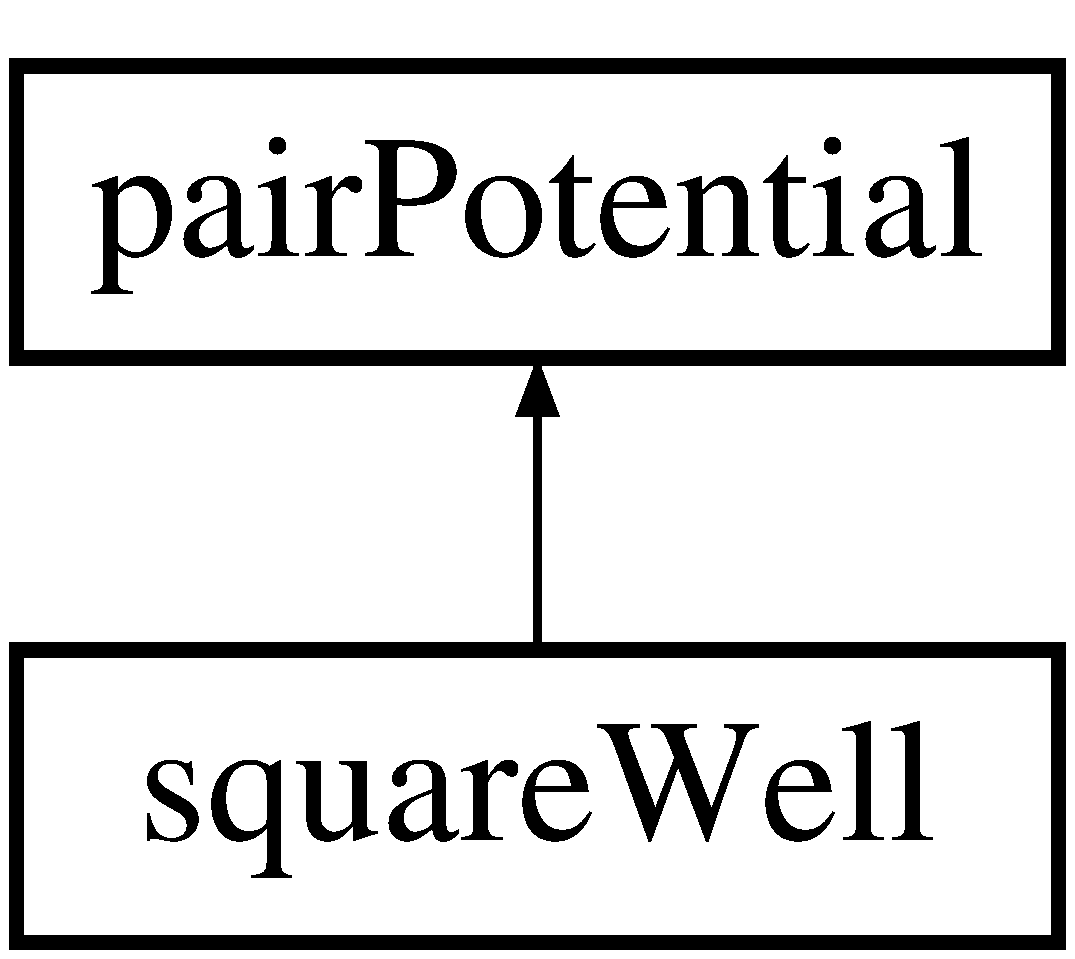
\includegraphics[height=2.000000cm]{classsquare_well}
\end{center}
\end{figure}
\subsection*{Public Member Functions}
\begin{DoxyCompactItemize}
\item 
\hyperlink{classsquare_well_aee8080c488f394e2157648849e0e4b43}{$\sim$square\-Well} ()
\item 
void \hyperlink{classsquare_well_aa8770429044914778c2f343e025e09cc}{set\-Parameters} (const std\-::vector$<$ double $>$ params)
\begin{DoxyCompactList}\small\item\em Set the parameters in the square-\/well equation. \end{DoxyCompactList}\item 
double \hyperlink{classsquare_well_af91d33913dd2ac3ce84e2cf18530f75d}{energy} (const \hyperlink{classatom}{atom} $\ast$a1, const \hyperlink{classatom}{atom} $\ast$a2, const std\-::vector$<$ double $>$ \&box)
\begin{DoxyCompactList}\small\item\em Return the energy of two particles. \end{DoxyCompactList}\item 
double \hyperlink{classsquare_well_a3a81297ea3a06f8a354c824a7ac5dc94}{tail\-Correction} (const double rho\-Bath)
\begin{DoxyCompactList}\small\item\em Tail correction for a square well potential always returns 0. \end{DoxyCompactList}\item 
double \hyperlink{classsquare_well_a82e1cc1009bd8e42e79e3c5f856f1b3b}{rcut} ()
\begin{DoxyCompactList}\small\item\em Return the value of r\-\_\-\{cut\} for this potential. \end{DoxyCompactList}\end{DoxyCompactItemize}
\subsection*{Additional Inherited Members}


\subsection{Detailed Description}
Square-\/well potential Parameters should be specified in the following order\-: \{ sigma, wellwidth, welldepth, Mtot \}. 

Definition at line 96 of file potentials.\-h.



\subsection{Constructor \& Destructor Documentation}
\hypertarget{classsquare_well_aee8080c488f394e2157648849e0e4b43}{\index{square\-Well@{square\-Well}!$\sim$square\-Well@{$\sim$square\-Well}}
\index{$\sim$square\-Well@{$\sim$square\-Well}!squareWell@{square\-Well}}
\subsubsection[{$\sim$square\-Well}]{\setlength{\rightskip}{0pt plus 5cm}square\-Well\-::$\sim$square\-Well (
\begin{DoxyParamCaption}
{}
\end{DoxyParamCaption}
)\hspace{0.3cm}{\ttfamily [inline]}}}\label{classsquare_well_aee8080c488f394e2157648849e0e4b43}


Definition at line 98 of file potentials.\-h.


\begin{DoxyCode}
98 \{;\}
\end{DoxyCode}


\subsection{Member Function Documentation}
\hypertarget{classsquare_well_af91d33913dd2ac3ce84e2cf18530f75d}{\index{square\-Well@{square\-Well}!energy@{energy}}
\index{energy@{energy}!squareWell@{square\-Well}}
\subsubsection[{energy}]{\setlength{\rightskip}{0pt plus 5cm}double square\-Well\-::energy (
\begin{DoxyParamCaption}
\item[{const {\bf atom} $\ast$}]{a1, }
\item[{const {\bf atom} $\ast$}]{a2, }
\item[{const std\-::vector$<$ double $>$ \&}]{box}
\end{DoxyParamCaption}
)\hspace{0.3cm}{\ttfamily [virtual]}}}\label{classsquare_well_af91d33913dd2ac3ce84e2cf18530f75d}


Return the energy of two particles. 


\begin{DoxyParams}[1]{Parameters}
\mbox{\tt in}  & {\em a1} & Atom 1 \\
\hline
\mbox{\tt in}  & {\em a2} & Atom 2 \\
\hline
\mbox{\tt in}  & {\em box} & Simulation box dimensions\\
\hline
\end{DoxyParams}
\begin{DoxyReturn}{Returns}
U(r) 
\end{DoxyReturn}


Implements \hyperlink{classpair_potential_a2b1e50ef9b6e50b01d89d31d5460ad76}{pair\-Potential}.



Definition at line 511 of file potentials.\-cpp.



References atom\-::m\-State, N\-U\-M\-\_\-\-I\-N\-F\-I\-N\-I\-T\-Y, pair\-Potential\-::params\-Are\-Set\-\_\-, pbc\-Dist2(), and atom\-::pos.


\begin{DoxyCode}
511                                                                                           \{
512     \textcolor{keywordflow}{if} (!\hyperlink{classpair_potential_a635755c0a952bfc05a4cfae230c3dbd2}{paramsAreSet\_}) \{
513         \textcolor{keywordflow}{throw} \hyperlink{classcustom_exception}{customException} (\textcolor{stringliteral}{"For squareWell parameters not set"});
514     \}
515 
516     \textcolor{keyword}{const} \textcolor{keywordtype}{double} r = sqrt(\hyperlink{utilities_8cpp_abb1db3a8a3ac46e044bbe7b2c5684c0a}{pbcDist2}(a1->\hyperlink{classatom_a3ae5f4880e7831d8b2c9fda72b4eb24a}{pos}, a2->\hyperlink{classatom_a3ae5f4880e7831d8b2c9fda72b4eb24a}{pos}, box));
517 
518     \textcolor{keywordtype}{int} mState = 0;
519     \textcolor{keywordflow}{if} (a1->\hyperlink{classatom_a3cb00c0c5b7533657e05af6ff4a42740}{mState} != 0) \{
520         mState = a1->\hyperlink{classatom_a3cb00c0c5b7533657e05af6ff4a42740}{mState};
521     \}
522     \textcolor{keywordflow}{if} (a2->\hyperlink{classatom_a3cb00c0c5b7533657e05af6ff4a42740}{mState} != 0) \{
523         mState = a2->\hyperlink{classatom_a3cb00c0c5b7533657e05af6ff4a42740}{mState};
524     \}
525 
526     \textcolor{keywordflow}{if} (r < sigmaM\_[mState]) \{
527         \textcolor{keywordflow}{return} \hyperlink{potentials_8h_ab94ab1d09e2291d03fe92a0e24a9d33b}{NUM\_INFINITY};
528     \} \textcolor{keywordflow}{else} \textcolor{keywordflow}{if} (r < rangeM\_[mState]) \{
529         \textcolor{keywordflow}{return} epsM\_[mState];
530     \} \textcolor{keywordflow}{else} \{
531         \textcolor{keywordflow}{return} 0.0;
532     \}
533 \}
\end{DoxyCode}
\hypertarget{classsquare_well_a82e1cc1009bd8e42e79e3c5f856f1b3b}{\index{square\-Well@{square\-Well}!rcut@{rcut}}
\index{rcut@{rcut}!squareWell@{square\-Well}}
\subsubsection[{rcut}]{\setlength{\rightskip}{0pt plus 5cm}double square\-Well\-::rcut (
\begin{DoxyParamCaption}
{}
\end{DoxyParamCaption}
)\hspace{0.3cm}{\ttfamily [virtual]}}}\label{classsquare_well_a82e1cc1009bd8e42e79e3c5f856f1b3b}


Return the value of r\-\_\-\{cut\} for this potential. 

\begin{DoxyReturn}{Returns}
r\-\_\-cut 
\end{DoxyReturn}


Implements \hyperlink{classpair_potential_abf4f8d231c5e2e36d72916d33dcd75f0}{pair\-Potential}.



Definition at line 551 of file potentials.\-cpp.



References pair\-Potential\-::params\-\_\-, and pair\-Potential\-::params\-Are\-Set\-\_\-.


\begin{DoxyCode}
551                          \{
552     \textcolor{keywordflow}{if} (!\hyperlink{classpair_potential_a635755c0a952bfc05a4cfae230c3dbd2}{paramsAreSet\_}) \{
553         \textcolor{keywordflow}{throw} \hyperlink{classcustom_exception}{customException} (\textcolor{stringliteral}{"For squareWell parameters not set"});
554     \} \textcolor{keywordflow}{else} \{
555         \textcolor{keywordflow}{return} (\hyperlink{classpair_potential_abf8ec8af983d6e9960bd149da099e883}{params\_}[1]);
556     \}
557 \}
\end{DoxyCode}
\hypertarget{classsquare_well_aa8770429044914778c2f343e025e09cc}{\index{square\-Well@{square\-Well}!set\-Parameters@{set\-Parameters}}
\index{set\-Parameters@{set\-Parameters}!squareWell@{square\-Well}}
\subsubsection[{set\-Parameters}]{\setlength{\rightskip}{0pt plus 5cm}void square\-Well\-::set\-Parameters (
\begin{DoxyParamCaption}
\item[{const std\-::vector$<$ double $>$}]{params}
\end{DoxyParamCaption}
)\hspace{0.3cm}{\ttfamily [virtual]}}}\label{classsquare_well_aa8770429044914778c2f343e025e09cc}


Set the parameters in the square-\/well equation. 


\begin{DoxyParams}[1]{Parameters}
\mbox{\tt in}  & {\em params} & Vector of inputs\-: \{sigma, width, epsilon, Mtot\} \\
\hline
\end{DoxyParams}


Implements \hyperlink{classpair_potential_ad4b237646f9de2ae9f95cc9350564bc5}{pair\-Potential}.



Definition at line 443 of file potentials.\-cpp.



References pair\-Potential\-::params\-\_\-, pair\-Potential\-::params\-Are\-Set\-\_\-, and pair\-Potential\-::use\-Tail\-Correction.


\begin{DoxyCode}
443                                                                  \{
444     \textcolor{keywordflow}{if} (params.size() != 4) \{
445         \textcolor{keywordflow}{throw} \hyperlink{classcustom_exception}{customException} (\textcolor{stringliteral}{"For squareWell must specify 4 parameters: sigma, width,
       epsilon, Mtot"});
446     \} \textcolor{keywordflow}{else} \{
447         \textcolor{keywordflow}{if} (params[0] < 0) \{
448             \textcolor{keywordflow}{throw} \hyperlink{classcustom_exception}{customException} (\textcolor{stringliteral}{"For squareWell, sigma >= 0"});
449         \}
450         \textcolor{keywordflow}{if} (params[1] < 0) \{
451             \textcolor{keywordflow}{throw} \hyperlink{classcustom_exception}{customException} (\textcolor{stringliteral}{"For squareWell, width >= 0"});
452         \}
453         \textcolor{keywordflow}{if} (params[2] < 0) \{
454             \textcolor{keywordflow}{throw} \hyperlink{classcustom_exception}{customException} (\textcolor{stringliteral}{"For squareWell, epsilon >= 0"});
455         \}
456         \textcolor{keywordflow}{if} (\textcolor{keywordtype}{int}(params[3]) < 1) \{
457             \textcolor{keywordflow}{throw} \hyperlink{classcustom_exception}{customException} (\textcolor{stringliteral}{"For squareWell, total expanded ensemble states, Mtot >=
       1"});
458         \}
459 
460         \hyperlink{classpair_potential_ab4b4538a7e13771f50a29aaac2443037}{useTailCorrection} = \textcolor{keyword}{false};
461 
462         \textcolor{comment}{// use a "constant volume" scheme to distribute the stages}
463         sigmaM\_.resize(\textcolor{keywordtype}{int}(params[3]), 0);
464         rangeM\_.resize(\textcolor{keywordtype}{int}(params[3]), 0);
465         \textcolor{keywordflow}{for} (\textcolor{keywordtype}{int} i = 0; i < sigmaM\_.size(); ++i) \{
466             \textcolor{keywordflow}{if} (i == 0) \{
467                 \textcolor{comment}{// fully inserted}
468                 sigmaM\_[i] = params[0];
469                 rangeM\_[i] = params[0] + params[1];
470             \} \textcolor{keywordflow}{else} \{
471                 \textcolor{comment}{// use volume scaling so each stage is separated from its neighbors by the same dV}
472                 \textcolor{keywordtype}{double} lastSigma = 0;
473                 \textcolor{keywordflow}{if} (i == 1) \{
474                     lastSigma = 0;
475                 \} \textcolor{keywordflow}{else} \{
476                     lastSigma = sigmaM\_[i-1];
477                 \}
478                 sigmaM\_[i] = pow(params[0]*params[0]*params[0]/(8.0*\textcolor{keywordtype}{int}(params[3])) + lastSigma*lastSigma*
      lastSigma, 1./3.);
479                 rangeM\_[i] = sigmaM\_[i] + params[1];
480             \}
481         \}
482 
483         \textcolor{comment}{// scale energy linearly across the stages}
484         epsM\_.resize(\textcolor{keywordtype}{int}(params[3]), 0);
485         \textcolor{keywordflow}{for} (\textcolor{keywordtype}{int} i = 0; i < epsM\_.size(); ++i) \{
486             \textcolor{keywordflow}{if} (i == 0) \{
487                 \textcolor{comment}{// fully inserted}
488                 epsM\_[i] = -params[2];
489             \} \textcolor{keywordflow}{else} \{
490                 epsM\_[i] = -i*(params[2]/int(params[3]));
491             \}
492         \}
493 
494         \textcolor{comment}{// save parameters as sigma, (sigma+wellWidth), -wellDepth to speed up energy calculation}
495         \hyperlink{classpair_potential_abf8ec8af983d6e9960bd149da099e883}{params\_} = params;
496         \hyperlink{classpair_potential_abf8ec8af983d6e9960bd149da099e883}{params\_}[1] = params[0] + params[1]; \textcolor{comment}{// max rcut}
497         \hyperlink{classpair_potential_abf8ec8af983d6e9960bd149da099e883}{params\_}[2] = -params[2];
498         \hyperlink{classpair_potential_a635755c0a952bfc05a4cfae230c3dbd2}{paramsAreSet\_} = \textcolor{keyword}{true};
499     \}
500 \}
\end{DoxyCode}
\hypertarget{classsquare_well_a3a81297ea3a06f8a354c824a7ac5dc94}{\index{square\-Well@{square\-Well}!tail\-Correction@{tail\-Correction}}
\index{tail\-Correction@{tail\-Correction}!squareWell@{square\-Well}}
\subsubsection[{tail\-Correction}]{\setlength{\rightskip}{0pt plus 5cm}double square\-Well\-::tail\-Correction (
\begin{DoxyParamCaption}
\item[{const double}]{rho\-Bath}
\end{DoxyParamCaption}
)\hspace{0.3cm}{\ttfamily [virtual]}}}\label{classsquare_well_a3a81297ea3a06f8a354c824a7ac5dc94}


Tail correction for a square well potential always returns 0. 


\begin{DoxyParams}[1]{Parameters}
\mbox{\tt in}  & {\em Number} & density of the surrounding fluid\\
\hline
\end{DoxyParams}
\begin{DoxyReturn}{Returns}
U\-\_\-tail 
\end{DoxyReturn}


Implements \hyperlink{classpair_potential_a5387d21d8d487d1d42e9eaf7cae9175b}{pair\-Potential}.



Definition at line 542 of file potentials.\-cpp.


\begin{DoxyCode}
542                                                       \{
543     \textcolor{keywordflow}{return} 0.0;
544 \}
\end{DoxyCode}


The documentation for this class was generated from the following files\-:\begin{DoxyCompactItemize}
\item 
/home/nam4/\-Desktop/sandbox/\-F\-H\-M\-C\-Simulation/src/\hyperlink{potentials_8h}{potentials.\-h}\item 
/home/nam4/\-Desktop/sandbox/\-F\-H\-M\-C\-Simulation/src/\hyperlink{potentials_8cpp}{potentials.\-cpp}\end{DoxyCompactItemize}

\hypertarget{classsquare_well_wall_z}{\section{square\-Well\-Wall\-Z Class Reference}
\label{classsquare_well_wall_z}\index{square\-Well\-Wall\-Z@{square\-Well\-Wall\-Z}}
}


Parallel square-\/well walls in the z-\/direction.  




{\ttfamily \#include $<$barrier.\-h$>$}

Inheritance diagram for square\-Well\-Wall\-Z\-:\begin{figure}[H]
\begin{center}
\leavevmode
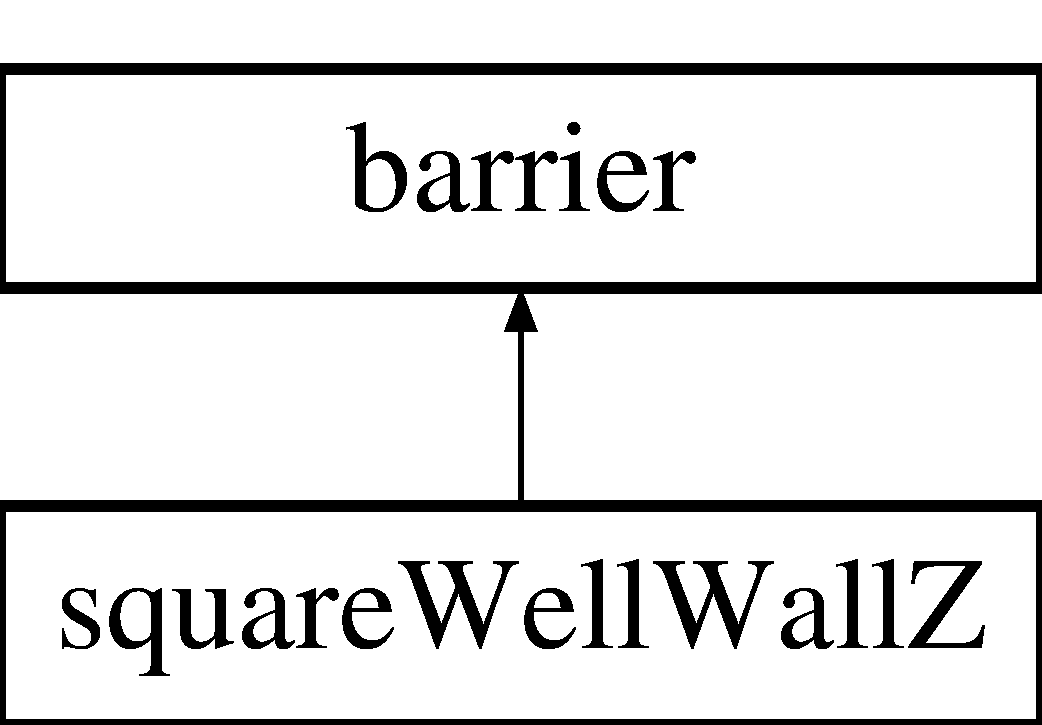
\includegraphics[height=2.000000cm]{classsquare_well_wall_z}
\end{center}
\end{figure}
\subsection*{Public Member Functions}
\begin{DoxyCompactItemize}
\item 
\hyperlink{classsquare_well_wall_z_a98e2785289630c78afcb0bc8a7fd24e1}{$\sim$square\-Well\-Wall\-Z} ()
\item 
\hyperlink{classsquare_well_wall_z_a9f4c4e2e118fd68c2591a4d6f06aa594}{square\-Well\-Wall\-Z} (const double lb, const double ub, const double sigma, const double range, const double eps, const int M=1)
\begin{DoxyCompactList}\small\item\em Instantiate a square well wall with boundaries in the +/-\/ z direction. \end{DoxyCompactList}\item 
bool \hyperlink{classsquare_well_wall_z_a10fc7a357ac1ec6bb0cd1d1e95570195}{inside} (const \hyperlink{classatom}{atom} $\ast$a1, const std\-::vector$<$ double $>$ \&box)
\begin{DoxyCompactList}\small\item\em Return whether or not a point falls between the walls (subject to a hard-\/sphere exclusion radius). \end{DoxyCompactList}\item 
double \hyperlink{classsquare_well_wall_z_a77c366eb9c10f6a68e3f633e9b64dc47}{energy} (const \hyperlink{classatom}{atom} $\ast$a1, const std\-::vector$<$ double $>$ \&box)
\begin{DoxyCompactList}\small\item\em Interaction energy with the wall. \end{DoxyCompactList}\end{DoxyCompactItemize}
\subsection*{Additional Inherited Members}


\subsection{Detailed Description}
Parallel square-\/well walls in the z-\/direction. 

Definition at line 45 of file barrier.\-h.



\subsection{Constructor \& Destructor Documentation}
\hypertarget{classsquare_well_wall_z_a98e2785289630c78afcb0bc8a7fd24e1}{\index{square\-Well\-Wall\-Z@{square\-Well\-Wall\-Z}!$\sim$square\-Well\-Wall\-Z@{$\sim$square\-Well\-Wall\-Z}}
\index{$\sim$square\-Well\-Wall\-Z@{$\sim$square\-Well\-Wall\-Z}!squareWellWallZ@{square\-Well\-Wall\-Z}}
\subsubsection[{$\sim$square\-Well\-Wall\-Z}]{\setlength{\rightskip}{0pt plus 5cm}square\-Well\-Wall\-Z\-::$\sim$square\-Well\-Wall\-Z (
\begin{DoxyParamCaption}
{}
\end{DoxyParamCaption}
)\hspace{0.3cm}{\ttfamily [inline]}}}\label{classsquare_well_wall_z_a98e2785289630c78afcb0bc8a7fd24e1}


Definition at line 47 of file barrier.\-h.


\begin{DoxyCode}
47 \{\};
\end{DoxyCode}
\hypertarget{classsquare_well_wall_z_a9f4c4e2e118fd68c2591a4d6f06aa594}{\index{square\-Well\-Wall\-Z@{square\-Well\-Wall\-Z}!square\-Well\-Wall\-Z@{square\-Well\-Wall\-Z}}
\index{square\-Well\-Wall\-Z@{square\-Well\-Wall\-Z}!squareWellWallZ@{square\-Well\-Wall\-Z}}
\subsubsection[{square\-Well\-Wall\-Z}]{\setlength{\rightskip}{0pt plus 5cm}square\-Well\-Wall\-Z\-::square\-Well\-Wall\-Z (
\begin{DoxyParamCaption}
\item[{const double}]{lb, }
\item[{const double}]{ub, }
\item[{const double}]{sigma, }
\item[{const double}]{range, }
\item[{const double}]{eps, }
\item[{const int}]{M = {\ttfamily 1}}
\end{DoxyParamCaption}
)}}\label{classsquare_well_wall_z_a9f4c4e2e118fd68c2591a4d6f06aa594}


Instantiate a square well wall with boundaries in the +/-\/ z direction. 

Expanded ensembles primarily scale the magnitude of interaction. The repulsive boundary scales with sigma at the boundary, but the attractive cutoff remains fixed relative to the boundary.


\begin{DoxyParams}[1]{Parameters}
\mbox{\tt in}  & {\em lb} & z-\/\-Position of the lower wall \\
\hline
\mbox{\tt in}  & {\em ub} & z-\/\-Position of the upper wall \\
\hline
\mbox{\tt in}  & {\em sigma} & Hard-\/sphere diameter the species this wall interacts with can approach within \\
\hline
\mbox{\tt in}  & {\em range} & Distance normal to the wall's surface where there is an interaction \\
\hline
\mbox{\tt in}  & {\em eps} & Magnitude of the wall interaction (U = -\/eps) \\
\hline
\mbox{\tt in}  & {\em M} & Total number of expanded ensemble states possible for this atom type (defaults to 1) \\
\hline
\end{DoxyParams}


Definition at line 563 of file barrier.\-cpp.



References barrier\-::\-M\-\_\-.


\begin{DoxyCode}
563                                                                                                            
                                    \{
564     \textcolor{keywordflow}{if} (lb >= ub) \{
565         \textcolor{keywordflow}{throw} \hyperlink{classcustom_exception}{customException} (\textcolor{stringliteral}{"squareWellWallZ must have lower bound < upper bound"});
566     \}
567     \textcolor{keywordflow}{if} (sigma < 0) \{
568         \textcolor{keywordflow}{throw} \hyperlink{classcustom_exception}{customException} (\textcolor{stringliteral}{"squareWellWallZ must have sigma >= 0"});
569     \}
570     \textcolor{keywordflow}{if} (range < 0) \{
571         \textcolor{keywordflow}{throw} \hyperlink{classcustom_exception}{customException} (\textcolor{stringliteral}{"squareWellWallZ must have range >= 0"});
572     \}
573     \textcolor{keywordflow}{if} (eps < 0) \{
574         \textcolor{keywordflow}{throw} \hyperlink{classcustom_exception}{customException} (\textcolor{stringliteral}{"squareWellWallZ must have epsilon >= 0"});
575     \}
576     \textcolor{keywordflow}{if} (sigma/2.0 >= range) \{
577         \textcolor{keywordflow}{throw} \hyperlink{classcustom_exception}{customException} (\textcolor{stringliteral}{"squareWellWallZ must have sigma/2 < range to have a finite
       range of interaction"});
578     \}
579     \textcolor{keywordflow}{if} (M < 1) \{
580         \textcolor{keywordflow}{throw} \hyperlink{classcustom_exception}{customException} (\textcolor{stringliteral}{"squareWellWallZ must have M >= 1"});
581     \}
582 
583     eps\_ = eps;
584     sigma\_ = sigma;
585     range\_ = range;
586     ub\_ = ub;
587     lb\_ = lb;
588     \hyperlink{classbarrier_a274cf283ffc97c22ffa9a4258369c400}{M\_} = M;
589 \}
\end{DoxyCode}


\subsection{Member Function Documentation}
\hypertarget{classsquare_well_wall_z_a77c366eb9c10f6a68e3f633e9b64dc47}{\index{square\-Well\-Wall\-Z@{square\-Well\-Wall\-Z}!energy@{energy}}
\index{energy@{energy}!squareWellWallZ@{square\-Well\-Wall\-Z}}
\subsubsection[{energy}]{\setlength{\rightskip}{0pt plus 5cm}double square\-Well\-Wall\-Z\-::energy (
\begin{DoxyParamCaption}
\item[{const {\bf atom} $\ast$}]{a1, }
\item[{const std\-::vector$<$ double $>$ \&}]{box}
\end{DoxyParamCaption}
)\hspace{0.3cm}{\ttfamily [virtual]}}}\label{classsquare_well_wall_z_a77c366eb9c10f6a68e3f633e9b64dc47}


Interaction energy with the wall. 

Sigma and epsilon are scaled linearly with expanded ensemble state.


\begin{DoxyParams}[1]{Parameters}
\mbox{\tt in}  & {\em a1} & Pointer to atom with position to test -\/ this does N\-O\-T need to be in the simulation box a priori \\
\hline
\mbox{\tt in}  & {\em box} & Simulation box \\
\hline
\end{DoxyParams}


Implements \hyperlink{classbarrier_a2d308cfd5709aa479d0b37733f1a0db7}{barrier}.



Definition at line 622 of file barrier.\-cpp.



References barrier\-::\-M\-\_\-, atom\-::m\-State, N\-U\-M\-\_\-\-I\-N\-F\-I\-N\-I\-T\-Y, pbc(), and atom\-::pos.


\begin{DoxyCode}
622                                                                                \{
623     std::vector < double > p = a1->\hyperlink{classatom_a3ae5f4880e7831d8b2c9fda72b4eb24a}{pos};
624     \hyperlink{utilities_8cpp_ad858a38f435e9a0ee890aa0f526714d2}{pbc} (p, box);
625     \textcolor{keywordtype}{double} U = 0.0;
626 
627     \textcolor{keywordtype}{double} sig = sigma\_, eps = eps\_;
628     \textcolor{keywordflow}{if} (a1->\hyperlink{classatom_a3cb00c0c5b7533657e05af6ff4a42740}{mState} > 0) \{
629         sig = (sigma\_/\hyperlink{classbarrier_a274cf283ffc97c22ffa9a4258369c400}{M\_})*a1->\hyperlink{classatom_a3cb00c0c5b7533657e05af6ff4a42740}{mState};
630         eps = (eps\_/\hyperlink{classbarrier_a274cf283ffc97c22ffa9a4258369c400}{M\_})*a1->\hyperlink{classatom_a3cb00c0c5b7533657e05af6ff4a42740}{mState};
631     \}
632     \textcolor{keywordflow}{if} (a1->\hyperlink{classatom_a3cb00c0c5b7533657e05af6ff4a42740}{mState} < 0 || a1->\hyperlink{classatom_a3cb00c0c5b7533657e05af6ff4a42740}{mState} > \hyperlink{classbarrier_a274cf283ffc97c22ffa9a4258369c400}{M\_}-1) \{
633         \textcolor{keywordflow}{throw} \hyperlink{classcustom_exception}{customException} (\textcolor{stringliteral}{"mState out of bounds for squareWellWallZ"});
634     \}
635 
636     \textcolor{comment}{// return infinity if out of bounds}
637     \textcolor{keywordflow}{if} (p[2] >= ub\_ - sig/2.0 || p[2] <= lb\_ + sig/2.0) \{
638         \textcolor{keywordflow}{return} \hyperlink{potentials_8h_ab94ab1d09e2291d03fe92a0e24a9d33b}{NUM\_INFINITY};
639     \}
640 
641     \textcolor{comment}{// interaction with top wall}
642     \textcolor{keywordflow}{if} (p[2] > ub\_ - range\_) \{
643         U += -eps;
644     \}
645 
646     \textcolor{comment}{// interaction with lower wall}
647     \textcolor{keywordflow}{if} (p[2] < lb\_ + range\_) \{
648         U += -eps;
649     \}
650 
651     \textcolor{keywordflow}{return} U;
652 \}
\end{DoxyCode}
\hypertarget{classsquare_well_wall_z_a10fc7a357ac1ec6bb0cd1d1e95570195}{\index{square\-Well\-Wall\-Z@{square\-Well\-Wall\-Z}!inside@{inside}}
\index{inside@{inside}!squareWellWallZ@{square\-Well\-Wall\-Z}}
\subsubsection[{inside}]{\setlength{\rightskip}{0pt plus 5cm}bool square\-Well\-Wall\-Z\-::inside (
\begin{DoxyParamCaption}
\item[{const {\bf atom} $\ast$}]{a1, }
\item[{const std\-::vector$<$ double $>$ \&}]{box}
\end{DoxyParamCaption}
)\hspace{0.3cm}{\ttfamily [virtual]}}}\label{classsquare_well_wall_z_a10fc7a357ac1ec6bb0cd1d1e95570195}


Return whether or not a point falls between the walls (subject to a hard-\/sphere exclusion radius). 

Sigma is scaled linearly with expanded ensemble state.


\begin{DoxyParams}[1]{Parameters}
\mbox{\tt in}  & {\em a1} & Pointer to atom with position to test -\/ this does N\-O\-T need to be in the simulation box a priori \\
\hline
\mbox{\tt in}  & {\em box} & Simulation box \\
\hline
\end{DoxyParams}


Implements \hyperlink{classbarrier_a948ebdcfac501cb75d1a1f045a7d9125}{barrier}.



Definition at line 597 of file barrier.\-cpp.



References barrier\-::\-M\-\_\-, atom\-::m\-State, pbc(), and atom\-::pos.


\begin{DoxyCode}
597                                                                              \{
598     std::vector < double > p = a1->\hyperlink{classatom_a3ae5f4880e7831d8b2c9fda72b4eb24a}{pos};
599     \hyperlink{utilities_8cpp_ad858a38f435e9a0ee890aa0f526714d2}{pbc} (p, box);
600 
601     \textcolor{keywordtype}{double} sig = sigma\_;
602     \textcolor{keywordflow}{if} (a1->\hyperlink{classatom_a3cb00c0c5b7533657e05af6ff4a42740}{mState} > 0) \{
603         sig = (sigma\_/\hyperlink{classbarrier_a274cf283ffc97c22ffa9a4258369c400}{M\_})*a1->\hyperlink{classatom_a3cb00c0c5b7533657e05af6ff4a42740}{mState};
604     \}
605     \textcolor{keywordflow}{if} (a1->\hyperlink{classatom_a3cb00c0c5b7533657e05af6ff4a42740}{mState} < 0 || a1->\hyperlink{classatom_a3cb00c0c5b7533657e05af6ff4a42740}{mState} > \hyperlink{classbarrier_a274cf283ffc97c22ffa9a4258369c400}{M\_}-1) \{
606         \textcolor{keywordflow}{throw} \hyperlink{classcustom_exception}{customException} (\textcolor{stringliteral}{"mState out of bounds for squareWellWallZ"});
607     \}
608 
609     \textcolor{keywordflow}{if} (p[2] >= ub\_ - sig/2.0 || p[2] <= lb\_ + sig/2.0) \{
610         \textcolor{keywordflow}{return} \textcolor{keyword}{false};
611     \} \textcolor{keywordflow}{else} \{
612         \textcolor{keywordflow}{return} \textcolor{keyword}{true};
613     \}
614 \}
\end{DoxyCode}


The documentation for this class was generated from the following files\-:\begin{DoxyCompactItemize}
\item 
/home/nam4/\-Desktop/sandbox/\-F\-H\-M\-C\-Simulation/src/\hyperlink{barrier_8h}{barrier.\-h}\item 
/home/nam4/\-Desktop/sandbox/\-F\-H\-M\-C\-Simulation/src/\hyperlink{barrier_8cpp}{barrier.\-cpp}\end{DoxyCompactItemize}

\hypertarget{classswap_particles}{\section{swap\-Particles Class Reference}
\label{classswap_particles}\index{swap\-Particles@{swap\-Particles}}
}


{\ttfamily \#include $<$swap.\-h$>$}

Inheritance diagram for swap\-Particles\-:\begin{figure}[H]
\begin{center}
\leavevmode
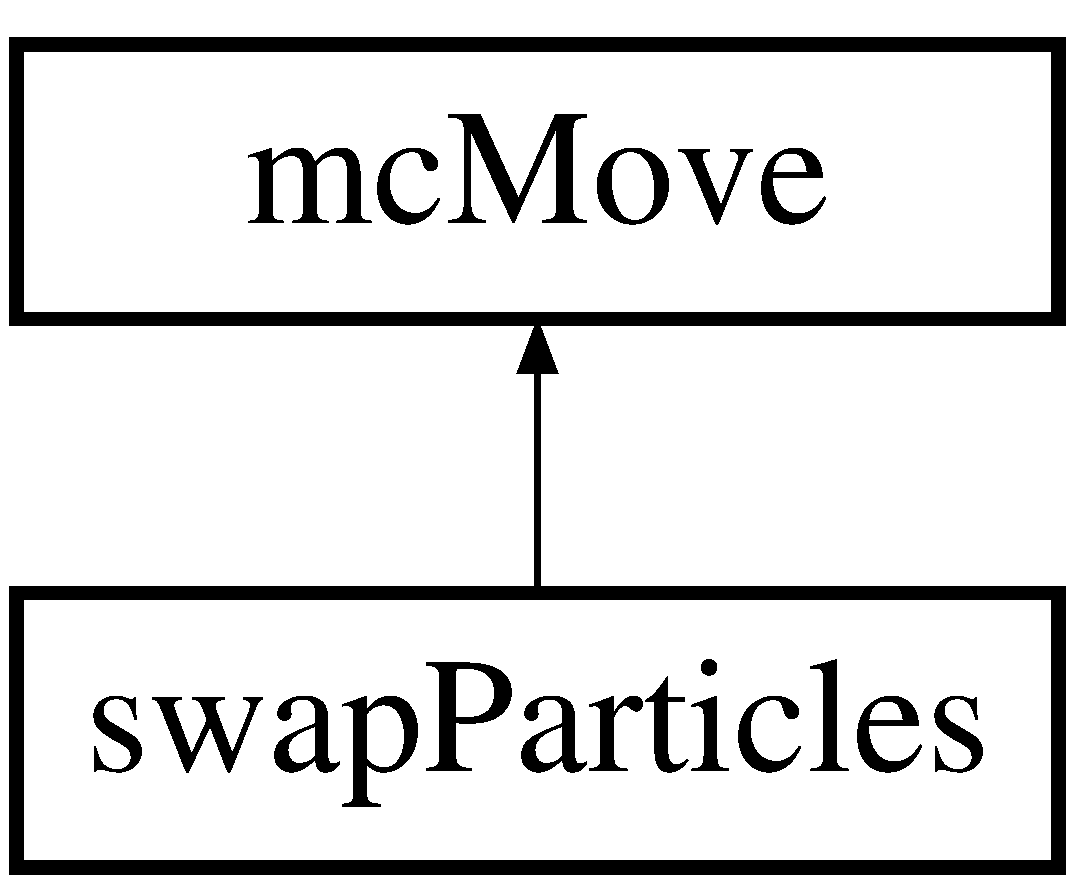
\includegraphics[height=2.000000cm]{classswap_particles}
\end{center}
\end{figure}
\subsection*{Public Member Functions}
\begin{DoxyCompactItemize}
\item 
\hyperlink{classswap_particles_a1c476913d5b129db6daf5a1a1a5dd209}{swap\-Particles} ()
\item 
\hyperlink{classswap_particles_aac7a7fb48c4ffd3809221fac7a7800a5}{swap\-Particles} (const int type\-Index1, const int type\-Index2, const std\-::string tag)
\begin{DoxyCompactList}\small\item\em Instantiate a new move, also give a name which is the combination of a user-\/defined tag + the particle indices it operates on. \end{DoxyCompactList}\item 
int \hyperlink{classswap_particles_ad8ca574f8e5308b6f0a5f3c7c2799209}{make} (\hyperlink{classsim_system}{sim\-System} \&sys)
\begin{DoxyCompactList}\small\item\em Swap two particles of different types in the system. \end{DoxyCompactList}\end{DoxyCompactItemize}
\subsection*{Additional Inherited Members}


\subsection{Detailed Description}


Definition at line 14 of file swap.\-h.



\subsection{Constructor \& Destructor Documentation}
\hypertarget{classswap_particles_a1c476913d5b129db6daf5a1a1a5dd209}{\index{swap\-Particles@{swap\-Particles}!swap\-Particles@{swap\-Particles}}
\index{swap\-Particles@{swap\-Particles}!swapParticles@{swap\-Particles}}
\subsubsection[{swap\-Particles}]{\setlength{\rightskip}{0pt plus 5cm}swap\-Particles\-::swap\-Particles (
\begin{DoxyParamCaption}
{}
\end{DoxyParamCaption}
)\hspace{0.3cm}{\ttfamily [inline]}}}\label{classswap_particles_a1c476913d5b129db6daf5a1a1a5dd209}


Definition at line 16 of file swap.\-h.



References mc\-Move\-::change\-N\-\_\-.


\begin{DoxyCode}
16 \{ \hyperlink{classmc_move_add8d6d08be181274a61c7463159ad929}{changeN\_} = \textcolor{keyword}{false}; \}
\end{DoxyCode}
\hypertarget{classswap_particles_aac7a7fb48c4ffd3809221fac7a7800a5}{\index{swap\-Particles@{swap\-Particles}!swap\-Particles@{swap\-Particles}}
\index{swap\-Particles@{swap\-Particles}!swapParticles@{swap\-Particles}}
\subsubsection[{swap\-Particles}]{\setlength{\rightskip}{0pt plus 5cm}swap\-Particles\-::swap\-Particles (
\begin{DoxyParamCaption}
\item[{const int}]{type\-Index1, }
\item[{const int}]{type\-Index2, }
\item[{const std\-::string}]{tag}
\end{DoxyParamCaption}
)\hspace{0.3cm}{\ttfamily [inline]}}}\label{classswap_particles_aac7a7fb48c4ffd3809221fac7a7800a5}


Instantiate a new move, also give a name which is the combination of a user-\/defined tag + the particle indices it operates on. 



Definition at line 17 of file swap.\-h.



References mc\-Move\-::change\-N\-\_\-, mc\-Move\-::name\-\_\-, and mc\-Move\-::type\-Index\-\_\-.



\subsection{Member Function Documentation}
\hypertarget{classswap_particles_ad8ca574f8e5308b6f0a5f3c7c2799209}{\index{swap\-Particles@{swap\-Particles}!make@{make}}
\index{make@{make}!swapParticles@{swap\-Particles}}
\subsubsection[{make}]{\setlength{\rightskip}{0pt plus 5cm}int swap\-Particles\-::make (
\begin{DoxyParamCaption}
\item[{{\bf sim\-System} \&}]{sys}
\end{DoxyParamCaption}
)\hspace{0.3cm}{\ttfamily [virtual]}}}\label{classswap_particles_ad8ca574f8e5308b6f0a5f3c7c2799209}


Swap two particles of different types in the system. 

All other information is stored in the \hyperlink{classsim_system}{sim\-System} object.


\begin{DoxyParams}[1]{Parameters}
\mbox{\tt in}  & {\em sys} & System object to attempt to swap particles in.\\
\hline
\end{DoxyParams}
\begin{DoxyReturn}{Returns}
M\-O\-V\-E\-\_\-\-S\-U\-C\-C\-E\-S\-S if particles are swapped, otherwise M\-O\-V\-E\-\_\-\-F\-A\-I\-L\-U\-R\-E if not. Will throw exceptions if there was an error. 
\end{DoxyReturn}


Implements \hyperlink{classmc_move_a2e377a628f9ecee5422fc8967d4924eb}{mc\-Move}.



Definition at line 10 of file swap.\-cpp.



References sim\-System\-::atoms, sim\-System\-::beta(), sim\-System\-::box(), calculate\-Bias(), sim\-System\-::delete\-Atom(), sim\-System\-::get\-Current\-M(), sim\-System\-::get\-Fractional\-Atom(), sim\-System\-::get\-Fractional\-Atom\-Type(), sim\-System\-::get\-Neighbor\-Atoms(), sim\-System\-::get\-Tot\-N(), sim\-System\-::get\-W\-A\-L\-A\-Bias(), sim\-System\-::increment\-Energy(), sim\-System\-::insert\-Atom(), M\-O\-V\-E\-\_\-\-F\-A\-I\-L\-U\-R\-E, M\-O\-V\-E\-\_\-\-S\-U\-C\-C\-E\-S\-S, sim\-System\-::n\-Species(), N\-U\-M\-\_\-\-I\-N\-F\-I\-N\-I\-T\-Y, sim\-System\-::num\-Species, atom\-::pos, sim\-System\-::ppot, rng(), R\-N\-G\-\_\-\-S\-E\-E\-D, sim\-System\-::species\-Barriers, sim\-System\-::tmmc\-Bias, mc\-Move\-::type\-Index\-\_\-, wala\-::update(), tmmc\-::update\-C(), sim\-System\-::use\-T\-M\-M\-C, sim\-System\-::use\-W\-A\-L\-A, and custom\-Exception\-::what().


\begin{DoxyCode}
10                                        \{
11     \textcolor{comment}{// Choose an atom of each type to try to exchange}
12     \textcolor{keywordtype}{int} n1Avail = sys.\hyperlink{classsim_system_a9eea865e6dc1cff377b1e79c4d9c23f0}{numSpecies}[\hyperlink{classmc_move_acb731965547b0326ef318ec96da8b46a}{typeIndex\_}];
13     \textcolor{keywordflow}{if} (sys.\hyperlink{classsim_system_a299fe4372e610b554eaaf5f5957b2dbc}{getCurrentM}() > 0 && sys.\hyperlink{classsim_system_a0500a9e84eecfbde7a98cf8a34f719d5}{getFractionalAtomType}() == 
      \hyperlink{classmc_move_acb731965547b0326ef318ec96da8b46a}{typeIndex\_}) \{
14         n1Avail++;
15     \}
16 
17     \textcolor{keywordtype}{int} n2Avail = sys.\hyperlink{classsim_system_a9eea865e6dc1cff377b1e79c4d9c23f0}{numSpecies}[typeIndex2\_];
18     \textcolor{keywordflow}{if} (sys.\hyperlink{classsim_system_a299fe4372e610b554eaaf5f5957b2dbc}{getCurrentM}() > 0 && sys.\hyperlink{classsim_system_a0500a9e84eecfbde7a98cf8a34f719d5}{getFractionalAtomType}() == typeIndex2\_
      ) \{
19         n2Avail++;
20     \}
21 
22     \textcolor{keywordflow}{if} (n1Avail < 1 || n2Avail < 1) \{
23         \textcolor{comment}{// Updates to biasing functions must be done even if at bounds}
24         \textcolor{keywordflow}{if} (sys.\hyperlink{classsim_system_aa83b00006b3919fb6e13f1bdeadece6a}{useWALA}) \{
25             sys.\hyperlink{classsim_system_a7cb5049de8b0988349e89e30e4000407}{getWALABias}()->\hyperlink{classwala_ab439e3f60bea6c54522a870b9ad67acf}{update}(sys.\hyperlink{classsim_system_a37dd827f4057049763351510147b9f1d}{getTotN}(), sys.
      \hyperlink{classsim_system_a299fe4372e610b554eaaf5f5957b2dbc}{getCurrentM}());
26         \}
27         \textcolor{keywordflow}{if} (sys.\hyperlink{classsim_system_aa474a50b6353c8897331b1ab1ce53ab1}{useTMMC}) \{
28             sys.\hyperlink{classsim_system_a13173f45a1e40a5f5a3552b0ebe15b54}{tmmcBias}->\hyperlink{classtmmc_ae067afc5b52af203b9d45f18d9737219}{updateC} (sys.\hyperlink{classsim_system_a37dd827f4057049763351510147b9f1d}{getTotN}(), sys.
      \hyperlink{classsim_system_a37dd827f4057049763351510147b9f1d}{getTotN}(), sys.\hyperlink{classsim_system_a299fe4372e610b554eaaf5f5957b2dbc}{getCurrentM}(), sys.\hyperlink{classsim_system_a299fe4372e610b554eaaf5f5957b2dbc}{getCurrentM}(), 0.0);
29         \}
30         \textcolor{keywordflow}{return} \hyperlink{moves_8h_a9832cf5fcfa8c0894545b591c9908e39}{MOVE\_FAILURE};
31     \}
32 
33     \textcolor{comment}{// Because the locations are effectively being swapped, it is fair to select a partially inserted atom
       to be involved}
34     \textcolor{keyword}{const} \textcolor{keywordtype}{int} a1 = (int) floor(\hyperlink{utilities_8cpp_a0f9542af4b475ac79cb679d7a8d14db0}{rng} (&\hyperlink{global_8h_a3f4e4ea24d5a5c66feae55d1f329c884}{RNG\_SEED}) * n1Avail);
35     \textcolor{keyword}{const} \textcolor{keywordtype}{int} a2 = (int) floor(\hyperlink{utilities_8cpp_a0f9542af4b475ac79cb679d7a8d14db0}{rng} (&\hyperlink{global_8h_a3f4e4ea24d5a5c66feae55d1f329c884}{RNG\_SEED}) * n2Avail);
36     \hyperlink{classatom}{atom} a1\_orig = sys.\hyperlink{classsim_system_a90421b19082f7fb8fc23b7264b1161e4}{atoms}[\hyperlink{classmc_move_acb731965547b0326ef318ec96da8b46a}{typeIndex\_}][a1], a1\_new = a1\_orig;
37     \hyperlink{classatom}{atom} a2\_orig = sys.\hyperlink{classsim_system_a90421b19082f7fb8fc23b7264b1161e4}{atoms}[typeIndex2\_][a2], a2\_new = a2\_orig;
38 
39     \textcolor{comment}{// Positions will be exchanged, but no other property should change}
40     a1\_new.\hyperlink{classatom_a3ae5f4880e7831d8b2c9fda72b4eb24a}{pos} = a2\_orig.\hyperlink{classatom_a3ae5f4880e7831d8b2c9fda72b4eb24a}{pos};
41     a2\_new.pos = a1\_orig.\hyperlink{classatom_a3ae5f4880e7831d8b2c9fda72b4eb24a}{pos};
42 
43     \textcolor{keyword}{const} std::vector < double > box = sys.\hyperlink{classsim_system_a8bff9dfb95b1b09a0fab2c1c485ade07}{box}();
44     \textcolor{keywordtype}{double} V = 1.0;
45     \textcolor{keywordflow}{for} (\textcolor{keywordtype}{unsigned} \textcolor{keywordtype}{int} i = 0; i < box.size(); ++i) \{
46         V *= box[i];
47     \}
48 
49     \textcolor{keywordtype}{double} dU = 0.0;
50 
51     \textcolor{keywordtype}{double} delEnergy = 0.0;
52     \textcolor{keywordflow}{for} (\textcolor{keywordtype}{unsigned} \textcolor{keywordtype}{int} spec = 0; spec < sys.\hyperlink{classsim_system_ab5e2e9b6204de15520302fe1d51688dd}{nSpecies}(); ++spec) \{
53         \textcolor{comment}{// Get positions of neighboring atoms around a1}
54         std::vector < atom* > neighborAtoms = sys.\hyperlink{classsim_system_a9b3aeefa22c3b50b5913df6eea753bc6}{getNeighborAtoms}(spec, 
      \hyperlink{classmc_move_acb731965547b0326ef318ec96da8b46a}{typeIndex\_}, &sys.\hyperlink{classsim_system_a90421b19082f7fb8fc23b7264b1161e4}{atoms}[\hyperlink{classmc_move_acb731965547b0326ef318ec96da8b46a}{typeIndex\_}][a1]);
55         \textcolor{keywordflow}{for} (\textcolor{keywordtype}{unsigned} \textcolor{keywordtype}{int} i = 0; i < neighborAtoms.size(); ++i) \{
56             \textcolor{keywordflow}{if} (neighborAtoms[i] == &sys.\hyperlink{classsim_system_a90421b19082f7fb8fc23b7264b1161e4}{atoms}[typeIndex2\_][a2]) \{
57                 \textcolor{comment}{// Skip their interaction as they were already deleted - this is fine because their net
       pairwise interaction doesn't change over the course of the simulation - this means we don't have to actually
       re-insert the other atom / get its interation somehow later}
58                 \textcolor{keywordflow}{continue};
59             \} \textcolor{keywordflow}{else} \{
60                 \textcolor{keywordflow}{try} \{
61                     delEnergy += sys.\hyperlink{classsim_system_ad2e290b5963f132e6a3a56cee35c8e9f}{ppot}[spec][\hyperlink{classmc_move_acb731965547b0326ef318ec96da8b46a}{typeIndex\_}]->energy(neighborAtoms[i], &sys.
      \hyperlink{classsim_system_a90421b19082f7fb8fc23b7264b1161e4}{atoms}[\hyperlink{classmc_move_acb731965547b0326ef318ec96da8b46a}{typeIndex\_}][a1], box);
62                 \} \textcolor{keywordflow}{catch} (\hyperlink{classcustom_exception}{customException}& ce) \{
63                     std::string a = \textcolor{stringliteral}{"Cannot delete because of energy error: "}, b = ce.
      \hyperlink{classcustom_exception_aeb6ab5848b038adfc68fde86a512f691}{what}();
64                     \textcolor{keywordflow}{throw} \hyperlink{classcustom_exception}{customException} (a+b);
65                 \}
66             \}
67         \}
68         \textcolor{comment}{// Add tail correction to potential energy -- only enable for fluid phase simulations}
69 \textcolor{preprocessor}{#ifdef FLUID\_PHASE\_SIMULATIONS}
70 \textcolor{preprocessor}{}        \textcolor{keywordflow}{if} (sys.\hyperlink{classsim_system_ad2e290b5963f132e6a3a56cee35c8e9f}{ppot}[spec][\hyperlink{classmc_move_acb731965547b0326ef318ec96da8b46a}{typeIndex\_}]->useTailCorrection) \{
71             \textcolor{keywordflow}{if} (!(sys.\hyperlink{classsim_system_a299fe4372e610b554eaaf5f5957b2dbc}{getCurrentM}() > 0 && sys.\hyperlink{classsim_system_a2ab77377c60e0e3109a6e875690b0ab7}{getFractionalAtom} () == &sys.
      \hyperlink{classsim_system_a90421b19082f7fb8fc23b7264b1161e4}{atoms}[\hyperlink{classmc_move_acb731965547b0326ef318ec96da8b46a}{typeIndex\_}][a1])) \{
72                 \textcolor{comment}{// Then a1 is not the partially inserted particle and tail interactions must be included}
73                 \textcolor{keywordflow}{if} (spec == typeIndex\_) \{
74                     \textcolor{keywordflow}{if} (sys.\hyperlink{classsim_system_a9eea865e6dc1cff377b1e79c4d9c23f0}{numSpecies}[spec]-1 > 0) \{
75                         delEnergy += sys.\hyperlink{classsim_system_ad2e290b5963f132e6a3a56cee35c8e9f}{ppot}[spec][\hyperlink{classmc_move_acb731965547b0326ef318ec96da8b46a}{typeIndex\_}]->tailCorrection((sys.
      \hyperlink{classsim_system_a9eea865e6dc1cff377b1e79c4d9c23f0}{numSpecies}[spec]-1)/V);
76                     \}
77                 \} \textcolor{keywordflow}{else} \{
78                     \textcolor{keywordflow}{if} (sys.\hyperlink{classsim_system_a9eea865e6dc1cff377b1e79c4d9c23f0}{numSpecies}[spec] > 0) \{
79                         delEnergy += sys.\hyperlink{classsim_system_ad2e290b5963f132e6a3a56cee35c8e9f}{ppot}[spec][\hyperlink{classmc_move_acb731965547b0326ef318ec96da8b46a}{typeIndex\_}]->tailCorrection(sys.
      \hyperlink{classsim_system_a9eea865e6dc1cff377b1e79c4d9c23f0}{numSpecies}[spec]/V);
80                     \}
81                 \}
82             \}
83         \}
84 \textcolor{preprocessor}{#endif}
85 \textcolor{preprocessor}{}    \}
86 
87     \textcolor{comment}{// Account for wall interaction energy}
88     delEnergy += sys.\hyperlink{classsim_system_a5ae652ff4519f39c3862abae32a9581b}{speciesBarriers}[\hyperlink{classmc_move_acb731965547b0326ef318ec96da8b46a}{typeIndex\_}].energy(&sys.
      \hyperlink{classsim_system_a90421b19082f7fb8fc23b7264b1161e4}{atoms}[typeIndex\_][a1], box);
89 
90     \textcolor{keywordflow}{for} (\textcolor{keywordtype}{unsigned} \textcolor{keywordtype}{int} spec = 0; spec < sys.\hyperlink{classsim_system_ab5e2e9b6204de15520302fe1d51688dd}{nSpecies}(); ++spec) \{
91         \textcolor{comment}{// Get positions of neighboring atoms around a2}
92         std::vector < atom* > neighborAtoms = sys.\hyperlink{classsim_system_a9b3aeefa22c3b50b5913df6eea753bc6}{getNeighborAtoms}(spec, typeIndex2\_, &sys.
      \hyperlink{classsim_system_a90421b19082f7fb8fc23b7264b1161e4}{atoms}[typeIndex2\_][a2]);
93         \textcolor{keywordflow}{for} (\textcolor{keywordtype}{unsigned} \textcolor{keywordtype}{int} i = 0; i < neighborAtoms.size(); ++i) \{
94             \textcolor{keywordflow}{if} (neighborAtoms[i] == &sys.\hyperlink{classsim_system_a90421b19082f7fb8fc23b7264b1161e4}{atoms}[typeIndex\_][a1]) \{
95                 \textcolor{comment}{// Skip their interaction as they were already deleted - this is fine because their net
       pairwise interaction doesn't change over the course of the simulation - this means we don't have to actually
       re-insert the other atom / get its interation somehow later}
96                 \textcolor{keywordflow}{continue};
97             \} \textcolor{keywordflow}{else} \{
98                 \textcolor{keywordflow}{try} \{
99                     delEnergy += sys.\hyperlink{classsim_system_ad2e290b5963f132e6a3a56cee35c8e9f}{ppot}[spec][typeIndex2\_]->energy(neighborAtoms[i], &sys.
      \hyperlink{classsim_system_a90421b19082f7fb8fc23b7264b1161e4}{atoms}[typeIndex2\_][a2], box);
100                 \} \textcolor{keywordflow}{catch} (\hyperlink{classcustom_exception}{customException}& ce) \{
101                     std::string a = \textcolor{stringliteral}{"Cannot delete because of energy error: "}, b = ce.
      \hyperlink{classcustom_exception_aeb6ab5848b038adfc68fde86a512f691}{what}();
102                     \textcolor{keywordflow}{throw} \hyperlink{classcustom_exception}{customException} (a+b);
103                 \}
104             \}
105         \}
106         \textcolor{comment}{// Add tail correction to potential energy -- only enable for fluid phase simulations}
107 \textcolor{preprocessor}{#ifdef FLUID\_PHASE\_SIMULATIONS}
108 \textcolor{preprocessor}{}        \textcolor{keywordflow}{if} (sys.\hyperlink{classsim_system_ad2e290b5963f132e6a3a56cee35c8e9f}{ppot}[spec][typeIndex2\_]->useTailCorrection) \{
109             \textcolor{keywordflow}{if} (!(sys.\hyperlink{classsim_system_a299fe4372e610b554eaaf5f5957b2dbc}{getCurrentM}() > 0 && sys.\hyperlink{classsim_system_a2ab77377c60e0e3109a6e875690b0ab7}{getFractionalAtom} () == &sys.
      \hyperlink{classsim_system_a90421b19082f7fb8fc23b7264b1161e4}{atoms}[typeIndex2\_][a2])) \{
110                 \textcolor{comment}{// Then a2 is not the partially inserted particle and tail interactions must be included}
111                 \textcolor{keywordflow}{if} (spec == typeIndex2\_) \{
112                     \textcolor{keywordflow}{if} (sys.\hyperlink{classsim_system_a9eea865e6dc1cff377b1e79c4d9c23f0}{numSpecies}[spec]-1 > 0) \{
113                         delEnergy += sys.\hyperlink{classsim_system_ad2e290b5963f132e6a3a56cee35c8e9f}{ppot}[spec][typeIndex2\_]->tailCorrection((sys.
      \hyperlink{classsim_system_a9eea865e6dc1cff377b1e79c4d9c23f0}{numSpecies}[spec]-1)/V);
114                     \}
115                 \} \textcolor{keywordflow}{else} \{
116                     \textcolor{keywordflow}{if} (sys.\hyperlink{classsim_system_a9eea865e6dc1cff377b1e79c4d9c23f0}{numSpecies}[spec] > 0) \{
117                         delEnergy += sys.\hyperlink{classsim_system_ad2e290b5963f132e6a3a56cee35c8e9f}{ppot}[spec][typeIndex2\_]->tailCorrection(sys.
      \hyperlink{classsim_system_a9eea865e6dc1cff377b1e79c4d9c23f0}{numSpecies}[spec]/V);
118                     \}
119                 \}
120             \}
121         \}
122 \textcolor{preprocessor}{#endif}
123 \textcolor{preprocessor}{}    \}
124 
125     \textcolor{comment}{// Account for wall interaction energy}
126     delEnergy += sys.\hyperlink{classsim_system_a5ae652ff4519f39c3862abae32a9581b}{speciesBarriers}[typeIndex2\_].energy(&sys.
      \hyperlink{classsim_system_a90421b19082f7fb8fc23b7264b1161e4}{atoms}[typeIndex2\_][a2], box);
127 
128     \textcolor{keywordtype}{double} insEnergy = 0.0;
129 
130     \textcolor{comment}{// Account for wall interaction energy first to be more efficient}
131     dU = sys.\hyperlink{classsim_system_a5ae652ff4519f39c3862abae32a9581b}{speciesBarriers}[\hyperlink{classmc_move_acb731965547b0326ef318ec96da8b46a}{typeIndex\_}].energy(&a1\_new, box);
132     \textcolor{keywordflow}{if} (dU < \hyperlink{potentials_8h_ab94ab1d09e2291d03fe92a0e24a9d33b}{NUM\_INFINITY}) \{
133         insEnergy += dU;
134     \} \textcolor{keywordflow}{else} \{
135         insEnergy = \hyperlink{potentials_8h_ab94ab1d09e2291d03fe92a0e24a9d33b}{NUM\_INFINITY};
136     \}
137 
138     \textcolor{keywordflow}{if} (insEnergy < \hyperlink{potentials_8h_ab94ab1d09e2291d03fe92a0e24a9d33b}{NUM\_INFINITY}) \{
139         \textcolor{comment}{// Account for wall interaction energy}
140         dU = sys.\hyperlink{classsim_system_a5ae652ff4519f39c3862abae32a9581b}{speciesBarriers}[typeIndex2\_].energy(&a2\_new, box);
141         \textcolor{keywordflow}{if} (dU < \hyperlink{potentials_8h_ab94ab1d09e2291d03fe92a0e24a9d33b}{NUM\_INFINITY}) \{
142             insEnergy += dU;
143         \} \textcolor{keywordflow}{else} \{
144             insEnergy = \hyperlink{potentials_8h_ab94ab1d09e2291d03fe92a0e24a9d33b}{NUM\_INFINITY};
145         \}
146     \}
147 
148     \textcolor{keywordflow}{if} (insEnergy < \hyperlink{potentials_8h_ab94ab1d09e2291d03fe92a0e24a9d33b}{NUM\_INFINITY}) \{
149         \textcolor{keywordflow}{for} (\textcolor{keywordtype}{unsigned} \textcolor{keywordtype}{int} spec = 0; spec < sys.\hyperlink{classsim_system_ab5e2e9b6204de15520302fe1d51688dd}{nSpecies}(); ++spec) \{
150             \textcolor{comment}{// Get positions of neighboring atoms around a1's (a2's) new (old) location}
151             std::vector < atom* > neighborAtoms = sys.\hyperlink{classsim_system_a9b3aeefa22c3b50b5913df6eea753bc6}{getNeighborAtoms}(spec, typeIndex\_, &
      a1\_new);
152             \textcolor{keywordflow}{for} (\textcolor{keywordtype}{unsigned} \textcolor{keywordtype}{int} i = 0; i < neighborAtoms.size(); ++i) \{
153                 \textcolor{comment}{// With these new "copy atoms" getNeighborAtoms can't guarantee it doesn't point to old
       self, so must check}
154                 \textcolor{keywordflow}{if} ((neighborAtoms[i] == &sys.\hyperlink{classsim_system_a90421b19082f7fb8fc23b7264b1161e4}{atoms}[typeIndex2\_][a2]) || (neighborAtoms[i] == &sys.
      \hyperlink{classsim_system_a90421b19082f7fb8fc23b7264b1161e4}{atoms}[\hyperlink{classmc_move_acb731965547b0326ef318ec96da8b46a}{typeIndex\_}][a1])) \{
155                     \textcolor{keywordflow}{continue};
156                 \} \textcolor{keywordflow}{else} \{
157                     \textcolor{keywordflow}{try} \{
158                         dU = sys.\hyperlink{classsim_system_ad2e290b5963f132e6a3a56cee35c8e9f}{ppot}[spec][\hyperlink{classmc_move_acb731965547b0326ef318ec96da8b46a}{typeIndex\_}]->energy(neighborAtoms[i], &a1\_new, 
      box);
159                     \} \textcolor{keywordflow}{catch} (\hyperlink{classcustom_exception}{customException}& ce) \{
160                         std::string a = \textcolor{stringliteral}{"Cannot insert because of energy error: "}, b = ce.
      \hyperlink{classcustom_exception_aeb6ab5848b038adfc68fde86a512f691}{what}();
161                         \textcolor{keywordflow}{throw} \hyperlink{classcustom_exception}{customException} (a+b);
162                     \}
163                     \textcolor{keywordflow}{if} (dU < \hyperlink{potentials_8h_ab94ab1d09e2291d03fe92a0e24a9d33b}{NUM\_INFINITY}) \{
164                         insEnergy += dU;
165                     \} \textcolor{keywordflow}{else} \{
166                         insEnergy = \hyperlink{potentials_8h_ab94ab1d09e2291d03fe92a0e24a9d33b}{NUM\_INFINITY};
167                         \textcolor{keywordflow}{break};
168                     \}
169                 \}
170             \}
171             \textcolor{keywordflow}{if} (insEnergy == \hyperlink{potentials_8h_ab94ab1d09e2291d03fe92a0e24a9d33b}{NUM\_INFINITY}) \textcolor{keywordflow}{break}; \textcolor{comment}{// Don't add anything if "infinite" already}
172 
173             \textcolor{comment}{// Add tail correction to potential energy -- only enable for fluid phase simulations}
174 \textcolor{preprocessor}{    #ifdef FLUID\_PHASE\_SIMULATIONS}
175 \textcolor{preprocessor}{}            \textcolor{keywordflow}{if} (sys.\hyperlink{classsim_system_ad2e290b5963f132e6a3a56cee35c8e9f}{ppot}[spec][typeIndex\_]->useTailCorrection) \{
176                 \textcolor{keywordflow}{if} (!(sys.\hyperlink{classsim_system_a299fe4372e610b554eaaf5f5957b2dbc}{getCurrentM}() > 0 && sys.\hyperlink{classsim_system_a2ab77377c60e0e3109a6e875690b0ab7}{getFractionalAtom} () == &sys
      .\hyperlink{classsim_system_a90421b19082f7fb8fc23b7264b1161e4}{atoms}[\hyperlink{classmc_move_acb731965547b0326ef318ec96da8b46a}{typeIndex\_}][a1])) \{
177                     \textcolor{comment}{// Then a1 is not the partially inserted particle and tail interactions must be
       included}
178                     \textcolor{keywordflow}{if} (spec == typeIndex\_) \{
179                         \textcolor{keywordflow}{if} (sys.\hyperlink{classsim_system_a9eea865e6dc1cff377b1e79c4d9c23f0}{numSpecies}[spec]-1 > 0) \{
180                             insEnergy += sys.\hyperlink{classsim_system_ad2e290b5963f132e6a3a56cee35c8e9f}{ppot}[spec][\hyperlink{classmc_move_acb731965547b0326ef318ec96da8b46a}{typeIndex\_}]->tailCorrection((sys.
      \hyperlink{classsim_system_a9eea865e6dc1cff377b1e79c4d9c23f0}{numSpecies}[spec]-1)/V); \textcolor{comment}{// Never infinite}
181                         \}
182                     \} \textcolor{keywordflow}{else} \{
183                         \textcolor{keywordflow}{if} (sys.\hyperlink{classsim_system_a9eea865e6dc1cff377b1e79c4d9c23f0}{numSpecies}[spec] > 0) \{
184                             insEnergy += sys.\hyperlink{classsim_system_ad2e290b5963f132e6a3a56cee35c8e9f}{ppot}[spec][\hyperlink{classmc_move_acb731965547b0326ef318ec96da8b46a}{typeIndex\_}]->tailCorrection(sys.
      \hyperlink{classsim_system_a9eea865e6dc1cff377b1e79c4d9c23f0}{numSpecies}[spec]/V); \textcolor{comment}{// Never infinite}
185                         \}
186                     \}
187                 \}
188             \}
189 \textcolor{preprocessor}{    #endif}
190 \textcolor{preprocessor}{}        \}
191     \}
192 
193     \textcolor{keywordflow}{if} (insEnergy < \hyperlink{potentials_8h_ab94ab1d09e2291d03fe92a0e24a9d33b}{NUM\_INFINITY}) \{
194         \textcolor{keywordflow}{for} (\textcolor{keywordtype}{unsigned} \textcolor{keywordtype}{int} spec = 0; spec < sys.\hyperlink{classsim_system_ab5e2e9b6204de15520302fe1d51688dd}{nSpecies}(); ++spec) \{
195             \textcolor{comment}{// Get positions of neighboring atoms around a2's (a1's) new (old) location}
196             std::vector < atom* > neighborAtoms = sys.\hyperlink{classsim_system_a9b3aeefa22c3b50b5913df6eea753bc6}{getNeighborAtoms}(spec, typeIndex2\_, &
      a2\_new);
197             \textcolor{keywordflow}{for} (\textcolor{keywordtype}{unsigned} \textcolor{keywordtype}{int} i = 0; i < neighborAtoms.size(); ++i) \{
198                 \textcolor{keywordflow}{if} ((neighborAtoms[i] == &sys.\hyperlink{classsim_system_a90421b19082f7fb8fc23b7264b1161e4}{atoms}[typeIndex\_][a1]) || (neighborAtoms[i] == &sys.
      \hyperlink{classsim_system_a90421b19082f7fb8fc23b7264b1161e4}{atoms}[typeIndex2\_][a2])) \{
199                     \textcolor{keywordflow}{continue};
200                 \} \textcolor{keywordflow}{else} \{
201                     \textcolor{keywordflow}{try} \{
202                         dU = sys.\hyperlink{classsim_system_ad2e290b5963f132e6a3a56cee35c8e9f}{ppot}[spec][typeIndex2\_]->energy(neighborAtoms[i], &a2\_new, box);
203                     \} \textcolor{keywordflow}{catch} (\hyperlink{classcustom_exception}{customException}& ce) \{
204                         std::string a = \textcolor{stringliteral}{"Cannot insert because of energy error: "}, b = ce.
      \hyperlink{classcustom_exception_aeb6ab5848b038adfc68fde86a512f691}{what}();
205                         \textcolor{keywordflow}{throw} \hyperlink{classcustom_exception}{customException} (a+b);
206                     \}
207                     \textcolor{keywordflow}{if} (dU < \hyperlink{potentials_8h_ab94ab1d09e2291d03fe92a0e24a9d33b}{NUM\_INFINITY}) \{
208                         insEnergy += dU;
209                     \} \textcolor{keywordflow}{else} \{
210                         insEnergy = \hyperlink{potentials_8h_ab94ab1d09e2291d03fe92a0e24a9d33b}{NUM\_INFINITY};
211                         \textcolor{keywordflow}{break};
212                     \}
213                 \}
214             \}
215             \textcolor{keywordflow}{if} (insEnergy == \hyperlink{potentials_8h_ab94ab1d09e2291d03fe92a0e24a9d33b}{NUM\_INFINITY}) \textcolor{keywordflow}{break}; \textcolor{comment}{// Don't add anything if "infinite" already}
216 
217             \textcolor{comment}{// Add tail correction to potential energy -- only enable for fluid phase simulations}
218 \textcolor{preprocessor}{    #ifdef FLUID\_PHASE\_SIMULATIONS}
219 \textcolor{preprocessor}{}            \textcolor{keywordflow}{if} (sys.\hyperlink{classsim_system_ad2e290b5963f132e6a3a56cee35c8e9f}{ppot}[spec][typeIndex2\_]->useTailCorrection) \{
220                 \textcolor{keywordflow}{if} (!(sys.\hyperlink{classsim_system_a299fe4372e610b554eaaf5f5957b2dbc}{getCurrentM}() > 0 && sys.\hyperlink{classsim_system_a2ab77377c60e0e3109a6e875690b0ab7}{getFractionalAtom} () == &sys
      .\hyperlink{classsim_system_a90421b19082f7fb8fc23b7264b1161e4}{atoms}[typeIndex2\_][a2])) \{
221                     \textcolor{comment}{// Then a2 is not the partially inserted particle and tail interactions must be
       included}
222                     \textcolor{keywordflow}{if} (spec == typeIndex2\_) \{
223                         \textcolor{keywordflow}{if} (sys.\hyperlink{classsim_system_a9eea865e6dc1cff377b1e79c4d9c23f0}{numSpecies}[spec]-1 > 0) \{
224                             insEnergy += sys.\hyperlink{classsim_system_ad2e290b5963f132e6a3a56cee35c8e9f}{ppot}[spec][typeIndex2\_]->tailCorrection((sys.
      \hyperlink{classsim_system_a9eea865e6dc1cff377b1e79c4d9c23f0}{numSpecies}[spec]-1)/V); \textcolor{comment}{// Never infinite}
225                         \}
226                     \} \textcolor{keywordflow}{else} \{
227                         \textcolor{keywordflow}{if} (sys.\hyperlink{classsim_system_a9eea865e6dc1cff377b1e79c4d9c23f0}{numSpecies}[spec] > 0) \{
228                             insEnergy += sys.\hyperlink{classsim_system_ad2e290b5963f132e6a3a56cee35c8e9f}{ppot}[spec][typeIndex2\_]->tailCorrection(sys.
      \hyperlink{classsim_system_a9eea865e6dc1cff377b1e79c4d9c23f0}{numSpecies}[spec]/V); \textcolor{comment}{// Never infinite}
229                         \}
230                     \}
231                 \}
232             \}
233 \textcolor{preprocessor}{    #endif}
234 \textcolor{preprocessor}{}        \}
235     \}
236 
237     \textcolor{comment}{// Biasing}
238     \textcolor{keywordtype}{double} p\_u = 0.0;
239     \textcolor{keywordflow}{if} (insEnergy < \hyperlink{potentials_8h_ab94ab1d09e2291d03fe92a0e24a9d33b}{NUM\_INFINITY}) \{
240         p\_u = exp(-sys.\hyperlink{classsim_system_a3eeec9678902f8d7fce4dad6064aaf4c}{beta}()*(insEnergy - delEnergy));
241     \}
242     \textcolor{keywordtype}{double} bias = \hyperlink{system_8cpp_acfe185adf03db047fd3753c0d788e0e3}{calculateBias}(sys, sys.\hyperlink{classsim_system_a37dd827f4057049763351510147b9f1d}{getTotN}(), sys.
      \hyperlink{classsim_system_a299fe4372e610b554eaaf5f5957b2dbc}{getCurrentM}());
243 
244     \textcolor{comment}{// TMMC gets updated the same way, regardless of whether the move gets accepted}
245     \textcolor{keywordflow}{if} (sys.\hyperlink{classsim_system_aa474a50b6353c8897331b1ab1ce53ab1}{useTMMC}) \{
246         sys.\hyperlink{classsim_system_a13173f45a1e40a5f5a3552b0ebe15b54}{tmmcBias}->\hyperlink{classtmmc_ae067afc5b52af203b9d45f18d9737219}{updateC} (sys.\hyperlink{classsim_system_a37dd827f4057049763351510147b9f1d}{getTotN}(), sys.\hyperlink{classsim_system_a37dd827f4057049763351510147b9f1d}{getTotN}(), sys.
      \hyperlink{classsim_system_a299fe4372e610b554eaaf5f5957b2dbc}{getCurrentM}(), sys.\hyperlink{classsim_system_a299fe4372e610b554eaaf5f5957b2dbc}{getCurrentM}(), std::min(1.0, p\_u));
247     \}
248 
249     \textcolor{keywordflow}{if} (\hyperlink{utilities_8cpp_a0f9542af4b475ac79cb679d7a8d14db0}{rng} (&\hyperlink{global_8h_a3f4e4ea24d5a5c66feae55d1f329c884}{RNG\_SEED}) < p\_u*bias) \{ \textcolor{comment}{// Swap the particles by deleting/reinserting}
250         sys.\hyperlink{classsim_system_a6ad31c08955b80873f865b3069618dcb}{incrementEnergy}(insEnergy - delEnergy);
251 
252         \textcolor{comment}{// -a1 completely}
253         \textcolor{keywordflow}{try} \{
254             sys.\hyperlink{classsim_system_acabf4fc5b5b90bba62e1449ddb3646c6}{deleteAtom}(typeIndex\_, a1, \textcolor{keyword}{true});
255         \} \textcolor{keywordflow}{catch} (\hyperlink{classcustom_exception}{customException} &ce) \{
256             std::string a = \textcolor{stringliteral}{"Failed to delete atom during swapping: "}, b = ce.
      \hyperlink{classcustom_exception_aeb6ab5848b038adfc68fde86a512f691}{what}();
257             \textcolor{keywordflow}{throw} \hyperlink{classcustom_exception}{customException} (a+b);
258         \}
259 
260         \textcolor{comment}{// -a2 completely}
261         \textcolor{keywordflow}{try} \{
262             sys.\hyperlink{classsim_system_acabf4fc5b5b90bba62e1449ddb3646c6}{deleteAtom}(typeIndex2\_, a2, \textcolor{keyword}{true});
263         \} \textcolor{keywordflow}{catch} (\hyperlink{classcustom_exception}{customException} &ce) \{
264             std::string a = \textcolor{stringliteral}{"Failed to delete atom during swapping: "}, b = ce.
      \hyperlink{classcustom_exception_aeb6ab5848b038adfc68fde86a512f691}{what}();
265             \textcolor{keywordflow}{throw} \hyperlink{classcustom_exception}{customException} (a+b);
266         \}
267 
268         \textcolor{comment}{// +a1\_new completely}
269         \textcolor{keywordflow}{try} \{
270             sys.\hyperlink{classsim_system_a0404e9435cc046d19b6bb990678ee069}{insertAtom}(typeIndex\_, &a1\_new, \textcolor{keyword}{true});
271         \} \textcolor{keywordflow}{catch} (\hyperlink{classcustom_exception}{customException} &ce) \{
272             std::string a = \textcolor{stringliteral}{"Failed to insert atom during swapping: "}, b = ce.
      \hyperlink{classcustom_exception_aeb6ab5848b038adfc68fde86a512f691}{what}();
273             \textcolor{keywordflow}{throw} \hyperlink{classcustom_exception}{customException} (a+b);
274         \}
275 
276         \textcolor{comment}{// +a2\_new completely}
277         \textcolor{keywordflow}{try} \{
278             sys.\hyperlink{classsim_system_a0404e9435cc046d19b6bb990678ee069}{insertAtom}(typeIndex2\_, &a2\_new, \textcolor{keyword}{true});
279         \} \textcolor{keywordflow}{catch} (\hyperlink{classcustom_exception}{customException} &ce) \{
280             std::string a = \textcolor{stringliteral}{"Failed to insert atom during swapping: "}, b = ce.
      \hyperlink{classcustom_exception_aeb6ab5848b038adfc68fde86a512f691}{what}();
281             \textcolor{keywordflow}{throw} \hyperlink{classcustom_exception}{customException} (a+b);
282         \}
283 
284         \textcolor{comment}{// Update Wang-Landau bias, if used}
285         \textcolor{keywordflow}{if} (sys.\hyperlink{classsim_system_aa83b00006b3919fb6e13f1bdeadece6a}{useWALA}) \{
286             sys.\hyperlink{classsim_system_a7cb5049de8b0988349e89e30e4000407}{getWALABias}()->\hyperlink{classwala_ab439e3f60bea6c54522a870b9ad67acf}{update}(sys.\hyperlink{classsim_system_a37dd827f4057049763351510147b9f1d}{getTotN}(), sys.
      \hyperlink{classsim_system_a299fe4372e610b554eaaf5f5957b2dbc}{getCurrentM}());
287         \}
288         \textcolor{keywordflow}{return} \hyperlink{moves_8h_ae8285cbddc5d21f73f49dcbad82a775a}{MOVE\_SUCCESS};
289     \}
290 
291     \textcolor{comment}{// Update Wang-Landau bias (even if moved failed), if used}
292     \textcolor{keywordflow}{if} (sys.\hyperlink{classsim_system_aa83b00006b3919fb6e13f1bdeadece6a}{useWALA}) \{
293         sys.\hyperlink{classsim_system_a7cb5049de8b0988349e89e30e4000407}{getWALABias}()->\hyperlink{classwala_ab439e3f60bea6c54522a870b9ad67acf}{update}(sys.\hyperlink{classsim_system_a37dd827f4057049763351510147b9f1d}{getTotN}(), sys.
      \hyperlink{classsim_system_a299fe4372e610b554eaaf5f5957b2dbc}{getCurrentM}());
294     \}
295 
296     \textcolor{keywordflow}{return} \hyperlink{moves_8h_a9832cf5fcfa8c0894545b591c9908e39}{MOVE\_FAILURE};
297 \}
\end{DoxyCode}


The documentation for this class was generated from the following files\-:\begin{DoxyCompactItemize}
\item 
/home/nam4/\-Desktop/sandbox/\-F\-H\-M\-C\-Simulation/src/\hyperlink{swap_8h}{swap.\-h}\item 
/home/nam4/\-Desktop/sandbox/\-F\-H\-M\-C\-Simulation/src/\hyperlink{swap_8cpp}{swap.\-cpp}\end{DoxyCompactItemize}

\hypertarget{classtabulated}{}\section{tabulated Class Reference}
\label{classtabulated}\index{tabulated@{tabulated}}


Tabulated Potential Parameters should be specified in the following order\+: \{ r\+\_\+cut, r\+\_\+shift, u\+\_\+shift, u\+\_\+infinity \}.  




{\ttfamily \#include $<$potentials.\+h$>$}

Inheritance diagram for tabulated\+:\begin{figure}[H]
\begin{center}
\leavevmode
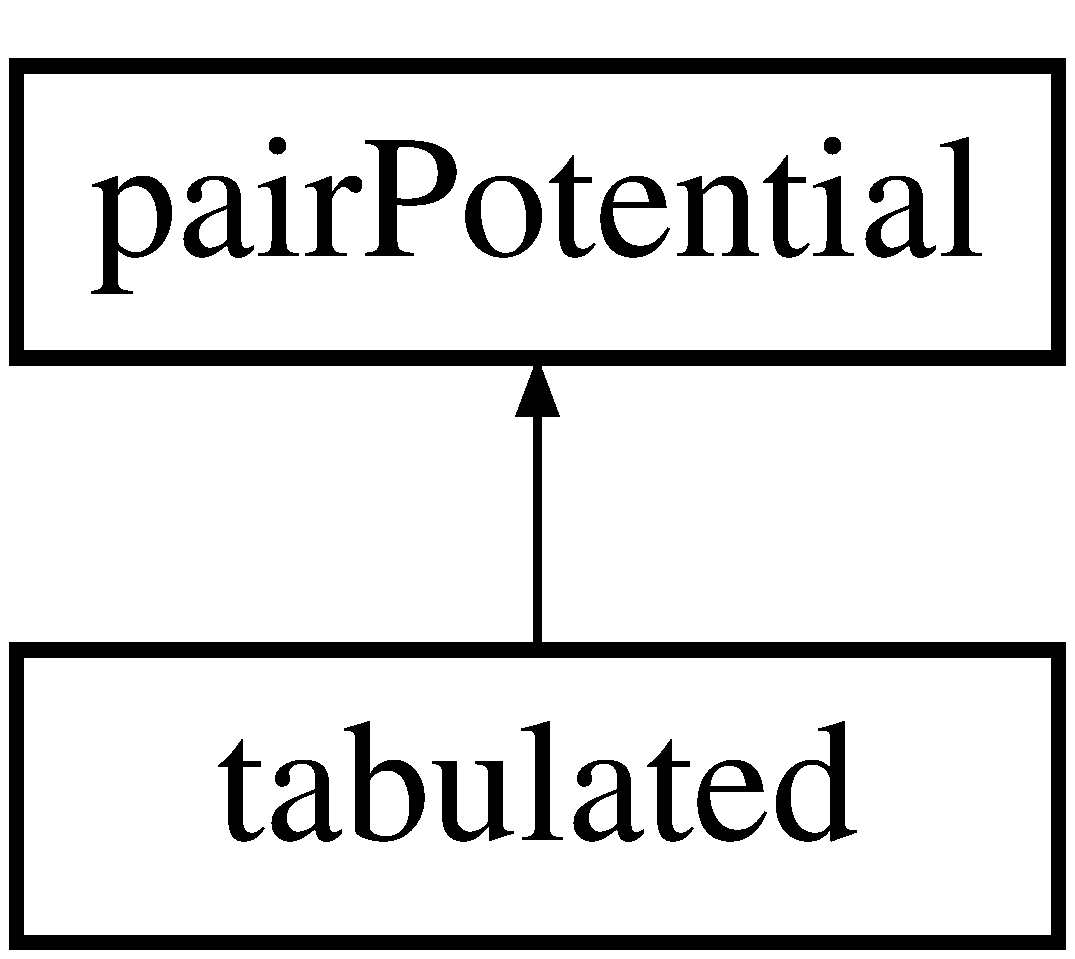
\includegraphics[height=2.000000cm]{classtabulated}
\end{center}
\end{figure}
\subsection*{Public Member Functions}
\begin{DoxyCompactItemize}
\item 
\hyperlink{classtabulated_a069eb60dc00583fd48b7488c9b9ada38}{$\sim$tabulated} ()
\item 
void \hyperlink{classtabulated_a6a52e8a5b99ddd16fcbd3e404c90f559}{set\+Parameters} (const std\+::vector$<$ double $>$ params)
\begin{DoxyCompactList}\small\item\em Set the parameters in the tabulated potential. \end{DoxyCompactList}\item 
void \hyperlink{classtabulated_ad3b3fb94b5db44e91d6768cfe21683c3}{load\+Potential} (std\+::string filename)
\begin{DoxyCompactList}\small\item\em Load a tabulated potential from an external file and store it internally. \end{DoxyCompactList}\item 
double \hyperlink{classtabulated_a09fdfccca3e19adb68da74f0baac7423}{energy} (const double r)
\begin{DoxyCompactList}\small\item\em Return the energy of two particles separate by a distance r. \end{DoxyCompactList}\item 
double \hyperlink{classtabulated_afb2936dfc0ba4255eb06f9d81e594dd2}{tail\+Correction} (const double rho\+Bath)
\begin{DoxyCompactList}\small\item\em Tail correction for a tabulated potential always returns 0 since no information about what the potential is after its cutoff radius. \end{DoxyCompactList}\item 
double \hyperlink{classtabulated_a1826f920afd53d74e17c8fa5253a2d2b}{rcut} ()
\begin{DoxyCompactList}\small\item\em Return the value of r\+\_\+\{cut\} for this potential. \end{DoxyCompactList}\end{DoxyCompactItemize}
\subsection*{Additional Inherited Members}


\subsection{Detailed Description}
Tabulated Potential Parameters should be specified in the following order\+: \{ r\+\_\+cut, r\+\_\+shift, u\+\_\+shift, u\+\_\+infinity \}. 

Definition at line 50 of file potentials.\+h.



\subsection{Constructor \& Destructor Documentation}
\hypertarget{classtabulated_a069eb60dc00583fd48b7488c9b9ada38}{}\index{tabulated@{tabulated}!````~tabulated@{$\sim$tabulated}}
\index{````~tabulated@{$\sim$tabulated}!tabulated@{tabulated}}
\subsubsection[{$\sim$tabulated()}]{\setlength{\rightskip}{0pt plus 5cm}tabulated\+::$\sim$tabulated (
\begin{DoxyParamCaption}
{}
\end{DoxyParamCaption}
)\hspace{0.3cm}{\ttfamily [inline]}}\label{classtabulated_a069eb60dc00583fd48b7488c9b9ada38}


Definition at line 56 of file potentials.\+h.


\begin{DoxyCode}
56 \{;\}
\end{DoxyCode}


\subsection{Member Function Documentation}
\hypertarget{classtabulated_a09fdfccca3e19adb68da74f0baac7423}{}\index{tabulated@{tabulated}!energy@{energy}}
\index{energy@{energy}!tabulated@{tabulated}}
\subsubsection[{energy(const double r)}]{\setlength{\rightskip}{0pt plus 5cm}double tabulated\+::energy (
\begin{DoxyParamCaption}
\item[{const double}]{r}
\end{DoxyParamCaption}
)\hspace{0.3cm}{\ttfamily [virtual]}}\label{classtabulated_a09fdfccca3e19adb68da74f0baac7423}


Return the energy of two particles separate by a distance r. 

Use linear interpolation to calculate energy from tabulated values


\begin{DoxyParams}[1]{Parameters}
\mbox{\tt in}  & {\em r} & Scalar separation, needs to be the minimum image \\
\hline
\end{DoxyParams}


Implements \hyperlink{classpair_potential_a43dc9c840e25dc76e76d6ad7947c165d}{pair\+Potential}.



Definition at line 180 of file potentials.\+cpp.



References pair\+Potential\+::params\+\_\+, and pair\+Potential\+::params\+Are\+Set\+\_\+.


\begin{DoxyCode}
180                                         \{
181                 \textcolor{keywordflow}{if} (!\hyperlink{classpair_potential_a635755c0a952bfc05a4cfae230c3dbd2}{paramsAreSet\_}) \{
182                                 \textcolor{keywordflow}{throw} \hyperlink{classcustom_exception}{customException} (\textcolor{stringliteral}{"For tabulated parameters not set"});
183                 \}
184                 
185                 \textcolor{keywordflow}{if} (r < \hyperlink{classpair_potential_abf8ec8af983d6e9960bd149da099e883}{params\_}[1]) \{
186                                 std::cerr<<\textcolor{stringliteral}{"distance r too small in energy calculation in tabulated
       potential. Returning value at r="}<<start<<std::endl;
187                 \} \textcolor{keywordflow}{else} \textcolor{keywordflow}{if} (r > \hyperlink{classpair_potential_abf8ec8af983d6e9960bd149da099e883}{params\_}[0]) \{
188                                 \textcolor{keywordflow}{return} \hyperlink{classpair_potential_abf8ec8af983d6e9960bd149da099e883}{params\_}[3];
189                 \} \textcolor{keywordflow}{else} \{
190                                 \textcolor{keyword}{const} \textcolor{keywordtype}{unsigned} \textcolor{keywordtype}{int} lowerIndex = floor((r-\hyperlink{classpair_potential_abf8ec8af983d6e9960bd149da099e883}{params\_}[1])/dr);
191                                 \textcolor{keyword}{const} \textcolor{keywordtype}{unsigned} \textcolor{keywordtype}{int} upperIndex = ceil((r-\hyperlink{classpair_potential_abf8ec8af983d6e9960bd149da099e883}{params\_}[1])/dr);
192                                 
193                                 \textcolor{keyword}{const} \textcolor{keywordtype}{double} upperFraction = (r-\hyperlink{classpair_potential_abf8ec8af983d6e9960bd149da099e883}{params\_}[1])/dr-lowerIndex;
194                                 \textcolor{keyword}{const} \textcolor{keywordtype}{double} lowerFraction = 1.0-upperFraction;
195                                 
196                                 \textcolor{keywordflow}{return} (lowerFraction*table[lowerIndex] + upperFraction*table[upperIndex] +
       \hyperlink{classpair_potential_abf8ec8af983d6e9960bd149da099e883}{params\_}[2]);
197                 \}
198 \}
\end{DoxyCode}
\hypertarget{classtabulated_ad3b3fb94b5db44e91d6768cfe21683c3}{}\index{tabulated@{tabulated}!load\+Potential@{load\+Potential}}
\index{load\+Potential@{load\+Potential}!tabulated@{tabulated}}
\subsubsection[{load\+Potential(std\+::string filename)}]{\setlength{\rightskip}{0pt plus 5cm}void tabulated\+::load\+Potential (
\begin{DoxyParamCaption}
\item[{std\+::string}]{filename}
\end{DoxyParamCaption}
)}\label{classtabulated_ad3b3fb94b5db44e91d6768cfe21683c3}


Load a tabulated potential from an external file and store it internally. 


\begin{DoxyParams}[1]{Parameters}
\mbox{\tt in}  & {\em filename} & Name of A\+S\+C\+I\+I file to read (r, U(r)) from \\
\hline
\end{DoxyParams}


Definition at line 127 of file potentials.\+cpp.



References file\+Exists(), pair\+Potential\+::params\+\_\+, and pair\+Potential\+::params\+Are\+Set\+\_\+.


\begin{DoxyCode}
128 \{
129                 std::cout<<\textcolor{stringliteral}{"Loading pair potential from file: "}<<filename<<std::endl;
130                 \textcolor{comment}{// first check, if file exists}
131                 \textcolor{keywordflow}{if} (\hyperlink{utilities_8cpp_a9d1e3672fd331d4185c1763c80226307}{fileExists}(filename))
132                 \{
133                                 std::cout<<\textcolor{stringliteral}{"File found, processing."}<<std::endl;
134                                 table.clear();
135                                 \textcolor{keywordtype}{double} r, pot;
136                                 \textcolor{keywordtype}{unsigned} \textcolor{keywordtype}{int} lineCounter = 0;
137                                 
138                                 std::ifstream inputData(filename.c\_str());
139                                 \textcolor{keywordflow}{while} (inputData>>r>>pot) \{
140                                                 \textcolor{keywordflow}{if} (lineCounter == 0) \{
141                                                                 start = r;
142                                                 \}
143                                                 \textcolor{keywordflow}{else} \textcolor{keywordflow}{if} (lineCounter == 1) \{
144                                                                 dr = r - start;
145                                                 \}
146                                                 
147                                                 table.push\_back(pot);
148                                                 lineCounter++;
149                                 \}
150                                 inputData.close();
151                                 
152                                 \textcolor{keywordflow}{if} (lineCounter < 2) \{
153                                                 \hyperlink{classpair_potential_a635755c0a952bfc05a4cfae230c3dbd2}{paramsAreSet\_} = \textcolor{keyword}{false};
154                                                 std::cerr<<\textcolor{stringliteral}{"Tabulated potential "}<<filename<<\textcolor{stringliteral}{" needs at
       least 2 entries, cannot setup potential."}<<std::endl;
155                                                 \textcolor{keywordflow}{return};
156                                 \}
157                                 
158                                 \textcolor{comment}{// if parameters are not set, set default parameters}
159                                 \textcolor{keywordflow}{if} (!\hyperlink{classpair_potential_a635755c0a952bfc05a4cfae230c3dbd2}{paramsAreSet\_}) \{
160                                                 \hyperlink{classpair_potential_abf8ec8af983d6e9960bd149da099e883}{params\_}.assign(4, 0.0);
161                                                 \hyperlink{classpair_potential_abf8ec8af983d6e9960bd149da099e883}{params\_}[0] = start + (table.size()-1)*dr;
162                                                 \hyperlink{classpair_potential_abf8ec8af983d6e9960bd149da099e883}{params\_}[1] = start;
163                                                 params\_[2] = 0.0;
164                                                 params\_[3] = 0.0;
165                                                 \hyperlink{classpair_potential_a635755c0a952bfc05a4cfae230c3dbd2}{paramsAreSet\_} = \textcolor{keyword}{true};
166                                 \}
167                 \}
168                 \textcolor{keywordflow}{else} \{
169                                 std::cerr<<\textcolor{stringliteral}{"File "}<<filename<<\textcolor{stringliteral}{" not found, cannot setup potential."}<<
      std::endl;
170                                 \hyperlink{classpair_potential_a635755c0a952bfc05a4cfae230c3dbd2}{paramsAreSet\_} = \textcolor{keyword}{false};
171                 \}
172 \}
\end{DoxyCode}
\hypertarget{classtabulated_a1826f920afd53d74e17c8fa5253a2d2b}{}\index{tabulated@{tabulated}!rcut@{rcut}}
\index{rcut@{rcut}!tabulated@{tabulated}}
\subsubsection[{rcut()}]{\setlength{\rightskip}{0pt plus 5cm}double tabulated\+::rcut (
\begin{DoxyParamCaption}
{}
\end{DoxyParamCaption}
)\hspace{0.3cm}{\ttfamily [virtual]}}\label{classtabulated_a1826f920afd53d74e17c8fa5253a2d2b}


Return the value of r\+\_\+\{cut\} for this potential. 

\begin{DoxyReturn}{Returns}
rcut 
\end{DoxyReturn}


Implements \hyperlink{classpair_potential_abf4f8d231c5e2e36d72916d33dcd75f0}{pair\+Potential}.



Definition at line 216 of file potentials.\+cpp.



References pair\+Potential\+::params\+\_\+, and pair\+Potential\+::params\+Are\+Set\+\_\+.


\begin{DoxyCode}
216                         \{
217                 \textcolor{keywordflow}{if} (!\hyperlink{classpair_potential_a635755c0a952bfc05a4cfae230c3dbd2}{paramsAreSet\_}) \{
218                                 \textcolor{keywordflow}{throw} \hyperlink{classcustom_exception}{customException} (\textcolor{stringliteral}{"For tabulated parameters not set"});
219                 \} \textcolor{keywordflow}{else} \{
220                                 \textcolor{keywordflow}{return} \hyperlink{classpair_potential_abf8ec8af983d6e9960bd149da099e883}{params\_}[0];
221                 \}
222 \}
\end{DoxyCode}
\hypertarget{classtabulated_a6a52e8a5b99ddd16fcbd3e404c90f559}{}\index{tabulated@{tabulated}!set\+Parameters@{set\+Parameters}}
\index{set\+Parameters@{set\+Parameters}!tabulated@{tabulated}}
\subsubsection[{set\+Parameters(const std\+::vector$<$ double $>$ params)}]{\setlength{\rightskip}{0pt plus 5cm}void tabulated\+::set\+Parameters (
\begin{DoxyParamCaption}
\item[{const std\+::vector$<$ double $>$}]{params}
\end{DoxyParamCaption}
)\hspace{0.3cm}{\ttfamily [virtual]}}\label{classtabulated_a6a52e8a5b99ddd16fcbd3e404c90f559}


Set the parameters in the tabulated potential. 


\begin{DoxyParams}[1]{Parameters}
\mbox{\tt in}  & {\em params} & Vector of inputs\+: \{r\+\_\+cut, r\+\_\+shift, u\+\_\+shift, u\+\_\+infinity\} \\
\hline
\end{DoxyParams}


Implements \hyperlink{classpair_potential_ad4b237646f9de2ae9f95cc9350564bc5}{pair\+Potential}.



Definition at line 107 of file potentials.\+cpp.



References pair\+Potential\+::params\+\_\+, pair\+Potential\+::params\+Are\+Set\+\_\+, and pair\+Potential\+::use\+Tail\+Correction.



Referenced by main().


\begin{DoxyCode}
107                                                                 \{
108                 \textcolor{keywordflow}{if} (params.size() != 4) \{
109                                 \textcolor{keywordflow}{throw} \hyperlink{classcustom_exception}{customException} (\textcolor{stringliteral}{"For tabulated must specify 4
       parameters: r\_cut, r\_shift, u\_shift, u\_infinity"});
110                 \} \textcolor{keywordflow}{else} \{
111                                 \textcolor{keywordflow}{if} (params[0] < 0) \{
112                                                 \textcolor{keywordflow}{throw} \hyperlink{classcustom_exception}{customException} (\textcolor{stringliteral}{"For tabulated, r\_cut
       > 0"});
113                                 \}
114                                 
115                                 \hyperlink{classpair_potential_a635755c0a952bfc05a4cfae230c3dbd2}{paramsAreSet\_} = \textcolor{keyword}{true};
116                                 \hyperlink{classpair_potential_abf8ec8af983d6e9960bd149da099e883}{params\_} = params;
117                                 
118                                 \hyperlink{classpair_potential_ab4b4538a7e13771f50a29aaac2443037}{useTailCorrection} = \textcolor{keyword}{false};
119                 \}
120 \}
\end{DoxyCode}
\hypertarget{classtabulated_afb2936dfc0ba4255eb06f9d81e594dd2}{}\index{tabulated@{tabulated}!tail\+Correction@{tail\+Correction}}
\index{tail\+Correction@{tail\+Correction}!tabulated@{tabulated}}
\subsubsection[{tail\+Correction(const double rho\+Bath)}]{\setlength{\rightskip}{0pt plus 5cm}double tabulated\+::tail\+Correction (
\begin{DoxyParamCaption}
\item[{const double}]{rho\+Bath}
\end{DoxyParamCaption}
)\hspace{0.3cm}{\ttfamily [virtual]}}\label{classtabulated_afb2936dfc0ba4255eb06f9d81e594dd2}


Tail correction for a tabulated potential always returns 0 since no information about what the potential is after its cutoff radius. 


\begin{DoxyParams}[1]{Parameters}
\mbox{\tt in}  & {\em Number} & density of the surrounding fluid\\
\hline
\end{DoxyParams}
\begin{DoxyReturn}{Returns}
U\+\_\+tail 
\end{DoxyReturn}


Implements \hyperlink{classpair_potential_a5387d21d8d487d1d42e9eaf7cae9175b}{pair\+Potential}.



Definition at line 207 of file potentials.\+cpp.


\begin{DoxyCode}
207                                                      \{
208                 \textcolor{keywordflow}{return} 0.0;
209 \}
\end{DoxyCode}


The documentation for this class was generated from the following files\+:\begin{DoxyCompactItemize}
\item 
/\+Users/nam4/\+Desktop/omcs/src/\hyperlink{potentials_8h}{potentials.\+h}\item 
/\+Users/nam4/\+Desktop/omcs/src/\hyperlink{potentials_8cpp}{potentials.\+cpp}\end{DoxyCompactItemize}

\hypertarget{classtmmc}{}\section{tmmc Class Reference}
\label{classtmmc}\index{tmmc@{tmmc}}


Transition Matrix Monte Carlo biasing class.  




{\ttfamily \#include $<$bias.\+h$>$}

\subsection*{Public Member Functions}
\begin{DoxyCompactItemize}
\item 
\hyperlink{classtmmc_a2dd6a666daae3a9b7c3978d8ecff887e}{tmmc} ()
\item 
\hyperlink{classtmmc_a643b39f7bd100470c9c632bc9ea7e45e}{tmmc} (const int Nmax, const int Nmin)
\begin{DoxyCompactList}\small\item\em Initialize the tmmc object. \end{DoxyCompactList}\item 
void \hyperlink{classtmmc_ab648f1ba2767c07fdccf9ac0e2eec8f6}{update\+C} (const int Nstart, const int Nend, const double pa)
\begin{DoxyCompactList}\small\item\em Update the collection matrix. \end{DoxyCompactList}\item 
void \hyperlink{classtmmc_a8e065523e9cc3c9628f91d3804cd201e}{calculate\+P\+I} ()
\begin{DoxyCompactList}\small\item\em Calculate the (natural logarithm of the) macrostate density matrix via the probability matrix. \end{DoxyCompactList}\item 
void \hyperlink{classtmmc_a059a91f0f2ebe78671b5f4fb8e1ab853}{print} (const std\+::string file\+Name, bool print\+C=false)
\begin{DoxyCompactList}\small\item\em Print the U\+N-\/\+N\+O\+R\+M\+A\+L\+I\+Z\+E\+D biasing function (ln\+P\+I) and possibly collection matrix to files. \end{DoxyCompactList}\item 
void \hyperlink{classtmmc_a7d9ee0505dc801cbff55bc35c3654a61}{read\+C} (const std\+::string file\+Name)
\begin{DoxyCompactList}\small\item\em Read the collection matrix from a file. \end{DoxyCompactList}\item 
void \hyperlink{classtmmc_a0c6c9f978b2093d1f4f6da7842093f3f}{readln\+P\+I} (const std\+::string file\+Name)
\begin{DoxyCompactList}\small\item\em Read the macrostate distribution (biasing function) from a file. \end{DoxyCompactList}\item 
void \hyperlink{classtmmc_a4bd3a47406bf765234e1cb3a391c79d5}{set\+Ln\+P\+I} (const std\+::vector$<$ double $>$ \&ln\+P\+Iguess)
\begin{DoxyCompactList}\small\item\em Blindly assign a guess of the macrostate distribution. \end{DoxyCompactList}\item 
bool \hyperlink{classtmmc_aa51f03f958dabefcff97be4a7c3b336c}{check\+Fully\+Visited} ()
\begin{DoxyCompactList}\small\item\em Check if the the collection matrix has been filled (i.\+e. \end{DoxyCompactList}\item 
const \hyperlink{bias_8h_a1ceb524363fcb94da0c64d297ea27438}{\+\_\+\+\_\+\+B\+I\+A\+S\+\_\+\+I\+N\+T\+\_\+\+T\+Y\+P\+E\+\_\+\+\_\+} \hyperlink{classtmmc_a7c006c0107ba4c1d52e75fc80d8581d6}{get\+Transition\+Address} (const int Nstart, const int Nend)
\begin{DoxyCompactList}\small\item\em For a given multidimensional array which has been cast into 1\+D, find the address that refers to a given transition. \end{DoxyCompactList}\item 
const \hyperlink{bias_8h_a1ceb524363fcb94da0c64d297ea27438}{\+\_\+\+\_\+\+B\+I\+A\+S\+\_\+\+I\+N\+T\+\_\+\+T\+Y\+P\+E\+\_\+\+\_\+} \hyperlink{classtmmc_aa93ae04c2712ef208ed4cb01b9dd1905}{get\+Address} (const int Nval)
\begin{DoxyCompactList}\small\item\em Get the address in ln\+P\+I that corresponds to a given macrostate. \end{DoxyCompactList}\item 
const double \hyperlink{classtmmc_afbcaaf974280aad6d78ca7e112438641}{get\+Bias} (const int address)
\end{DoxyCompactItemize}


\subsection{Detailed Description}
Transition Matrix Monte Carlo biasing class. 

Definition at line 23 of file bias.\+h.



\subsection{Constructor \& Destructor Documentation}
\hypertarget{classtmmc_a2dd6a666daae3a9b7c3978d8ecff887e}{}\index{tmmc@{tmmc}!tmmc@{tmmc}}
\index{tmmc@{tmmc}!tmmc@{tmmc}}
\subsubsection[{tmmc()}]{\setlength{\rightskip}{0pt plus 5cm}tmmc\+::tmmc (
\begin{DoxyParamCaption}
{}
\end{DoxyParamCaption}
)\hspace{0.3cm}{\ttfamily [inline]}}\label{classtmmc_a2dd6a666daae3a9b7c3978d8ecff887e}


Definition at line 25 of file bias.\+h.


\begin{DoxyCode}
25 \{\};
\end{DoxyCode}
\hypertarget{classtmmc_a643b39f7bd100470c9c632bc9ea7e45e}{}\index{tmmc@{tmmc}!tmmc@{tmmc}}
\index{tmmc@{tmmc}!tmmc@{tmmc}}
\subsubsection[{tmmc(const int Nmax, const int Nmin)}]{\setlength{\rightskip}{0pt plus 5cm}tmmc\+::tmmc (
\begin{DoxyParamCaption}
\item[{const int}]{Nmax, }
\item[{const int}]{Nmin}
\end{DoxyParamCaption}
)}\label{classtmmc_a643b39f7bd100470c9c632bc9ea7e45e}


Initialize the tmmc object. 


\begin{DoxyParams}[1]{Parameters}
\mbox{\tt in}  & {\em n\+Spec} & Number of species in the simulation. \\
\hline
\mbox{\tt in}  & {\em Nmax} & Upper bound for total number of particles. \\
\hline
\mbox{\tt in}  & {\em Nmin} & Lower bound for total number of particles. \\
\hline
\end{DoxyParams}


Definition at line 11 of file bias.\+cpp.



References \+\_\+\+\_\+\+B\+I\+A\+S\+\_\+\+I\+N\+T\+\_\+\+T\+Y\+P\+E\+\_\+\+\_\+.


\begin{DoxyCode}
11                                           \{     
12                 \textcolor{keywordflow}{if} (Nmin > Nmax) \{
13                                 \textcolor{keywordflow}{throw} \hyperlink{classcustom_exception}{customException} (\textcolor{stringliteral}{"Nmin > Nmax in TMMC bias"});
14                 \}
15                 \hyperlink{bias_8h_a1ceb524363fcb94da0c64d297ea27438}{\_\_BIAS\_INT\_TYPE\_\_} size = (Nmax - Nmin + 1);
16                 Nmin\_ = Nmin;
17                 Nmax\_ = Nmax;
18                 
19                 \textcolor{comment}{// attempt to allocate memory for collection matrix and initializes it all to 0}
20                 \textcolor{keywordflow}{try} \{
21                                 C\_.resize(3*size, 0);
22                 \} \textcolor{keywordflow}{catch} (\textcolor{keyword}{const} std::bad\_alloc &ce) \{
23                                 \textcolor{keywordflow}{throw} \hyperlink{classcustom_exception}{customException} (\textcolor{stringliteral}{"Out of memory, cannot allocate space
       for collection matrix in tmmc"});
24                 \}
25 
26                 \textcolor{comment}{// attempt to allocate memory for probability matrix and initializes it all to 0}
27                 \textcolor{keywordflow}{try} \{
28                                 P\_.resize(3*size, 0);
29                 \} \textcolor{keywordflow}{catch} (\textcolor{keyword}{const} std::bad\_alloc &ce) \{
30                                 \textcolor{keywordflow}{throw} \hyperlink{classcustom_exception}{customException} (\textcolor{stringliteral}{"Out of memory, cannot allocate space
       for probability matrix in tmmc"});
31                 \}
32                 
33                 \textcolor{comment}{// attempt to allocate memory for lnPI matrix and initializes it all to 0}
34                 \textcolor{keywordflow}{try} \{
35                                 lnPI\_.resize(size, 0.0);
36                 \} \textcolor{keywordflow}{catch} (\textcolor{keyword}{const} std::bad\_alloc &ce) \{
37                                 \textcolor{keywordflow}{throw} \hyperlink{classcustom_exception}{customException} (\textcolor{stringliteral}{"Out of memory, cannot allocate space
       for macrostate distribution matrix in tmmc"});
38                 \}
39 \}
\end{DoxyCode}


\subsection{Member Function Documentation}
\hypertarget{classtmmc_a8e065523e9cc3c9628f91d3804cd201e}{}\index{tmmc@{tmmc}!calculate\+P\+I@{calculate\+P\+I}}
\index{calculate\+P\+I@{calculate\+P\+I}!tmmc@{tmmc}}
\subsubsection[{calculate\+P\+I()}]{\setlength{\rightskip}{0pt plus 5cm}void tmmc\+::calculate\+P\+I (
\begin{DoxyParamCaption}
{}
\end{DoxyParamCaption}
)}\label{classtmmc_a8e065523e9cc3c9628f91d3804cd201e}


Calculate the (natural logarithm of the) macrostate density matrix via the probability matrix. 



Definition at line 116 of file bias.\+cpp.



References \+\_\+\+\_\+\+B\+I\+A\+S\+\_\+\+I\+N\+T\+\_\+\+T\+Y\+P\+E\+\_\+\+\_\+, get\+Transition\+Address(), and sstr.



Referenced by main().


\begin{DoxyCode}
116                         \{
117                 \textcolor{keywordflow}{for} (\hyperlink{bias_8h_a1ceb524363fcb94da0c64d297ea27438}{\_\_BIAS\_INT\_TYPE\_\_} i = 0; i < C\_.size(); i += 3) \{
118                                 \textcolor{keywordtype}{double} sum = 0.0;
119                                 \textcolor{keywordflow}{for} (\textcolor{keywordtype}{unsigned} \textcolor{keywordtype}{int} j = 0; j < 3; ++j) \{
120                                                 sum += C\_[i+j];
121                                 \}
122                                 \textcolor{keywordflow}{if} (sum > 0) \{
123                                                 \textcolor{keywordflow}{for} (\textcolor{keywordtype}{unsigned} \textcolor{keywordtype}{int} j = 0; j < 3; ++j) \{
124                                                                 P\_[i+j] = C\_[i+j] / sum;
125                                                 \}
126                                 \} \textcolor{keywordflow}{else} \{
127                                                 \textcolor{comment}{// This state has not been visited at all if sum = 0. 
       However, at high system densities this could be the "correct"}
128                                                 \textcolor{comment}{// result so this error may need to be discarded later in
       favor of:}
129                                                 \textcolor{comment}{// P\_[i+j] = 0;}
130                                                 \textcolor{comment}{// However, having this throw an exception is also a good
       way to find that upper bound where the system is completely packed}
131                                                 \textcolor{comment}{// so I will keep it this way for now.}
132                                                 \textcolor{keywordflow}{throw} \hyperlink{classcustom_exception}{customException} (\textcolor{stringliteral}{"Cannot compute TMMC
       macrostate distribution because probability matrix contains zeros"});
133                                 \}
134                 \}
135                 
136                 \textcolor{comment}{// Reset first value to zero just to start fresh. Since only ratios matter this is
       perfectly fair.}
137                 lnPI\_[0] = 0.0;
138                 \hyperlink{bias_8h_a1ceb524363fcb94da0c64d297ea27438}{\_\_BIAS\_INT\_TYPE\_\_} address1, address2;
139                 \textcolor{keywordflow}{for} (\hyperlink{bias_8h_a1ceb524363fcb94da0c64d297ea27438}{\_\_BIAS\_INT\_TYPE\_\_} i = 0; i < lnPI\_.size()-1; ++i) \{
140                                 address1 = \hyperlink{classtmmc_a7c006c0107ba4c1d52e75fc80d8581d6}{getTransitionAddress}(Nmin\_+i, Nmin\_+i+1);
141                                 address2 = \hyperlink{classtmmc_a7c006c0107ba4c1d52e75fc80d8581d6}{getTransitionAddress}(Nmin\_+i+1, Nmin\_+i);
142                                 \textcolor{keywordflow}{if} (!(P\_[address1] > 0) || !(P\_[address2] > 0)) \{
143                                                 \textcolor{keywordflow}{throw} \hyperlink{classcustom_exception}{customException} (\textcolor{stringliteral}{"Cannot compute TMMC
       macrostate distribution because probability matrix contains zeros at address: P["}+
      \hyperlink{utilities_8h_a8feb627efa8e8113cdf95f9a6151a088}{sstr}(address1)+\textcolor{stringliteral}{"] = "}+\hyperlink{utilities_8h_a8feb627efa8e8113cdf95f9a6151a088}{sstr}(P\_[address1])+\textcolor{stringliteral}{", P["}+\hyperlink{utilities_8h_a8feb627efa8e8113cdf95f9a6151a088}{sstr}(address2)+\textcolor{stringliteral}{"] = "}+
      \hyperlink{utilities_8h_a8feb627efa8e8113cdf95f9a6151a088}{sstr}(P\_[address2]));
144                                 \}
145                                 lnPI\_[i+1] = lnPI\_[i] + log(P\_[address1]/P\_[address2]); \textcolor{comment}{// this is why P\_
       cannot be zero}
146                 \}
147 \}
\end{DoxyCode}
\hypertarget{classtmmc_aa51f03f958dabefcff97be4a7c3b336c}{}\index{tmmc@{tmmc}!check\+Fully\+Visited@{check\+Fully\+Visited}}
\index{check\+Fully\+Visited@{check\+Fully\+Visited}!tmmc@{tmmc}}
\subsubsection[{check\+Fully\+Visited()}]{\setlength{\rightskip}{0pt plus 5cm}bool tmmc\+::check\+Fully\+Visited (
\begin{DoxyParamCaption}
{}
\end{DoxyParamCaption}
)}\label{classtmmc_aa51f03f958dabefcff97be4a7c3b336c}


Check if the the collection matrix has been filled (i.\+e. 

contains no zeros, except when crossing imposed bounds). Technically, if in an ideal gas state, d\+U $\sim$ 0 so pacc = 1.\+0, therefore probability of remaining in same state is 0. However, this matrix should be considered filled, if transitions to N+1 and N-\/1 for each N are found (except at bounds). 

Definition at line 46 of file bias.\+cpp.



References \+\_\+\+\_\+\+B\+I\+A\+S\+\_\+\+I\+N\+T\+\_\+\+T\+Y\+P\+E\+\_\+\+\_\+.



Referenced by main().


\begin{DoxyCode}
46                               \{
47                 \textcolor{keywordflow}{for} (\hyperlink{bias_8h_a1ceb524363fcb94da0c64d297ea27438}{\_\_BIAS\_INT\_TYPE\_\_} i = 0; i < C\_.size(); i += 3) \{
48                                 \textcolor{keywordflow}{if} (i == 0) \{
49                                                 \textcolor{comment}{// lower bound, so only +1 move must be sampled}
50                                                 \textcolor{keywordflow}{if} (!(C\_[i+1] > 0)) \{
51                                                                 \textcolor{keywordflow}{return} \textcolor{keyword}{false};
52                                                 \}                                               
53                                 \} \textcolor{keywordflow}{else} \textcolor{keywordflow}{if} (i == C\_.size()-3) \{
54                                                 \textcolor{comment}{// upper bound, so only -1 move must be sampled}
55                                                 \textcolor{keywordflow}{if} (!(C\_[i+2] > 0)) \{
56                                                                 \textcolor{keywordflow}{return} \textcolor{keyword}{false};
57                                                 \}
58                                 \} \textcolor{keywordflow}{else} \{
59                                                 \textcolor{comment}{// midpoints, both +1 and -1 moves must be sampled}
60                                                 \textcolor{keywordflow}{if} (!(C\_[i+1] > 0) || !(C\_[i+2] > 0)) \{
61                                                                 \textcolor{keywordflow}{return} \textcolor{keyword}{false};
62                                                 \}
63                                 \}
64                 \}
65                 \textcolor{keywordflow}{return} \textcolor{keyword}{true};
66 \}
\end{DoxyCode}
\hypertarget{classtmmc_aa93ae04c2712ef208ed4cb01b9dd1905}{}\index{tmmc@{tmmc}!get\+Address@{get\+Address}}
\index{get\+Address@{get\+Address}!tmmc@{tmmc}}
\subsubsection[{get\+Address(const int Nval)}]{\setlength{\rightskip}{0pt plus 5cm}const {\bf \+\_\+\+\_\+\+B\+I\+A\+S\+\_\+\+I\+N\+T\+\_\+\+T\+Y\+P\+E\+\_\+\+\_\+} tmmc\+::get\+Address (
\begin{DoxyParamCaption}
\item[{const int}]{Nval}
\end{DoxyParamCaption}
)}\label{classtmmc_aa93ae04c2712ef208ed4cb01b9dd1905}


Get the address in ln\+P\+I that corresponds to a given macrostate. 


\begin{DoxyParams}[1]{Parameters}
\mbox{\tt in}  & {\em Nval} & Number of total atoms \\
\hline
\end{DoxyParams}


Definition at line 95 of file bias.\+cpp.



References \+\_\+\+\_\+\+B\+I\+A\+S\+\_\+\+I\+N\+T\+\_\+\+T\+Y\+P\+E\+\_\+\+\_\+.



Referenced by calculate\+Bias().


\begin{DoxyCode}
95                                                         \{
96                 \hyperlink{bias_8h_a1ceb524363fcb94da0c64d297ea27438}{\_\_BIAS\_INT\_TYPE\_\_} x = Nval - Nmin\_;
97                 \textcolor{keywordflow}{return} x;
98 \}
\end{DoxyCode}
\hypertarget{classtmmc_afbcaaf974280aad6d78ca7e112438641}{}\index{tmmc@{tmmc}!get\+Bias@{get\+Bias}}
\index{get\+Bias@{get\+Bias}!tmmc@{tmmc}}
\subsubsection[{get\+Bias(const int address)}]{\setlength{\rightskip}{0pt plus 5cm}const double tmmc\+::get\+Bias (
\begin{DoxyParamCaption}
\item[{const int}]{address}
\end{DoxyParamCaption}
)\hspace{0.3cm}{\ttfamily [inline]}}\label{classtmmc_afbcaaf974280aad6d78ca7e112438641}


Definition at line 37 of file bias.\+h.



Referenced by calculate\+Bias().


\begin{DoxyCode}
37 \{ \textcolor{keywordflow}{return} -lnPI\_[address]; \}
\end{DoxyCode}
\hypertarget{classtmmc_a7c006c0107ba4c1d52e75fc80d8581d6}{}\index{tmmc@{tmmc}!get\+Transition\+Address@{get\+Transition\+Address}}
\index{get\+Transition\+Address@{get\+Transition\+Address}!tmmc@{tmmc}}
\subsubsection[{get\+Transition\+Address(const int Nstart, const int Nend)}]{\setlength{\rightskip}{0pt plus 5cm}const {\bf \+\_\+\+\_\+\+B\+I\+A\+S\+\_\+\+I\+N\+T\+\_\+\+T\+Y\+P\+E\+\_\+\+\_\+} tmmc\+::get\+Transition\+Address (
\begin{DoxyParamCaption}
\item[{const int}]{Nstart, }
\item[{const int}]{Nend}
\end{DoxyParamCaption}
)}\label{classtmmc_a7c006c0107ba4c1d52e75fc80d8581d6}


For a given multidimensional array which has been cast into 1\+D, find the address that refers to a given transition. 


\begin{DoxyParams}[1]{Parameters}
\mbox{\tt in}  & {\em Nstart} & Number of total species initially (before M\+C move) \\
\hline
\mbox{\tt in}  & {\em Nend} & Number of total species (in order) after the M\+C move \\
\hline
\end{DoxyParams}


Definition at line 74 of file bias.\+cpp.



References \+\_\+\+\_\+\+B\+I\+A\+S\+\_\+\+I\+N\+T\+\_\+\+T\+Y\+P\+E\+\_\+\+\_\+.



Referenced by calculate\+P\+I(), and update\+C().


\begin{DoxyCode}
74                                                                                     \{
75                 \textcolor{comment}{// Layout of y = [0, +1, -1] }
76                 \textcolor{keywordtype}{int} addOrSubtract = (Nend - Nstart), y = 0;
77                 \textcolor{keywordflow}{if} (addOrSubtract == 0) \{
78                                 y = 0;
79                 \} \textcolor{keywordflow}{else} \textcolor{keywordflow}{if} (addOrSubtract == 1) \{
80                                 y = 1;
81                 \} \textcolor{keywordflow}{else} \textcolor{keywordflow}{if} (addOrSubtract == -1) \{
82                                 y = 2;
83                 \} \textcolor{keywordflow}{else} \{
84                                 \textcolor{keywordflow}{throw} \hyperlink{classcustom_exception}{customException} (\textcolor{stringliteral}{"Illegal addOrSubtract value"});
85                 \}
86                 \hyperlink{bias_8h_a1ceb524363fcb94da0c64d297ea27438}{\_\_BIAS\_INT\_TYPE\_\_} x = Nstart - Nmin\_;
87                 \textcolor{keywordflow}{return} x*3 + y;
88 \}
\end{DoxyCode}
\hypertarget{classtmmc_a059a91f0f2ebe78671b5f4fb8e1ab853}{}\index{tmmc@{tmmc}!print@{print}}
\index{print@{print}!tmmc@{tmmc}}
\subsubsection[{print(const std\+::string file\+Name, bool print\+C=false)}]{\setlength{\rightskip}{0pt plus 5cm}void tmmc\+::print (
\begin{DoxyParamCaption}
\item[{const std\+::string}]{file\+Name, }
\item[{bool}]{print\+C = {\ttfamily false}}
\end{DoxyParamCaption}
)}\label{classtmmc_a059a91f0f2ebe78671b5f4fb8e1ab853}


Print the U\+N-\/\+N\+O\+R\+M\+A\+L\+I\+Z\+E\+D biasing function (ln\+P\+I) and possibly collection matrix to files. 

Will overwrite the files if another with that name exists. Prints in net\+C\+D\+F format if enabled.


\begin{DoxyParams}[1]{Parameters}
\mbox{\tt in}  & {\em file\+Name} & Name of the file to print to. Will append with \char`\"{}\+\_\+ln\+P\+I\char`\"{} and \char`\"{}\+\_\+\+C\char`\"{} for biasing function and collection matrix, respectively. \\
\hline
\mbox{\tt in}  & {\em print\+C} & Defaults to false, but if true will also print the collection matrix. \\
\hline
\end{DoxyParams}


Definition at line 157 of file bias.\+cpp.



References sstr.



Referenced by main().


\begin{DoxyCode}
157                                                        \{
158 \textcolor{preprocessor}{#ifdef NETCDF\_CAPABLE}
159                 \textcolor{comment}{// Print collection matrix}
160                 \textcolor{keywordflow}{if} (printC) \{
161                                 \textcolor{keyword}{const} std::string name = fileName + \textcolor{stringliteral}{"\_C.nc"}
162                                 NcFile outFile(name.c\_str(), NcFile::replace);
163                                 NcDim probDim = outFile.addDim(\textcolor{stringliteral}{"vectorized\_position"}, C\_.size());
164                                 NcVar probVar = outFile.addVar(\textcolor{stringliteral}{"C"}, ncDouble, probDim);
165                                 \textcolor{keyword}{const} std::string dummyName = \textcolor{stringliteral}{"number\_species:"};
166                                 probVar.putAtt(dummyName.c\_str(), \hyperlink{utilities_8h_a8feb627efa8e8113cdf95f9a6151a088}{sstr}(nSpec\_).c\_str());
167                                 \textcolor{keyword}{const} std::string attName = \textcolor{stringliteral}{"species\_total\_upper\_bound:"};
168                                 probVar.putAtt(attName.c\_str(), \hyperlink{utilities_8h_a8feb627efa8e8113cdf95f9a6151a088}{sstr}(Nmax\_).c\_str());
169                                 \textcolor{keyword}{const} std::string attName = \textcolor{stringliteral}{"species\_total\_lower\_bound:"};
170                                 probVar.putAtt(attName.c\_str(), \hyperlink{utilities_8h_a8feb627efa8e8113cdf95f9a6151a088}{sstr}(Nmin\_).c\_str());
171                                 probVar.putVar(&C\_[0]);
172                 \}
173                 
174                 \textcolor{comment}{// Print lnPI (bias) matrix}
175                 \textcolor{keyword}{const} std::string name = fileName + \textcolor{stringliteral}{"\_lnPI.nc"}
176                 NcFile outFile(name.c\_str(), NcFile::replace);
177                 NcDim probDim = outFile.addDim(\textcolor{stringliteral}{"vectorized\_position"}, lnPI\_.size());
178                 NcVar probVar = outFile.addVar(\textcolor{stringliteral}{"lnPI"}, ncDouble, probDim);
179                 \textcolor{keyword}{const} std::string attName = \textcolor{stringliteral}{"species\_total\_upper\_bound:"};
180                 probVar.putAtt(attName.c\_str(), \hyperlink{utilities_8h_a8feb627efa8e8113cdf95f9a6151a088}{sstr}(Nmax\_).c\_str());
181                 \textcolor{keyword}{const} std::string attName = \textcolor{stringliteral}{"species\_total\_lower\_bound:"};
182                 probVar.putAtt(attName.c\_str(), \hyperlink{utilities_8h_a8feb627efa8e8113cdf95f9a6151a088}{sstr}(Nmin\_).c\_str());
183                 probVar.putVar(&lnPI\_[0]);
184 \textcolor{preprocessor}{#else}
185                 \textcolor{comment}{// Print collection matrix}
186                 \textcolor{keywordflow}{if} (printC) \{
187                                 std::ofstream of;
188                                 of.open(fileName+\textcolor{stringliteral}{"\_C.dat"}, std::ofstream::out);
189                                 of << \textcolor{stringliteral}{"# Collection matrix in single row (vectorized) notation."} << 
      std::endl;
190                                 of << \textcolor{stringliteral}{"# species\_total\_upper\_bound: "} << Nmax\_ << std::endl;
191                                 of << \textcolor{stringliteral}{"# species\_total\_lower\_bound: "} << Nmin\_ << std::endl;
192                                 \textcolor{keywordflow}{for} (\textcolor{keywordtype}{long} \textcolor{keywordtype}{long} \textcolor{keywordtype}{int} i = 0; i < C\_.size(); ++i) \{
193                                                 of << C\_[i] << std::endl;
194                                 \}
195                                 of.close();
196                 \}
197                 
198                 \textcolor{comment}{// Print lnPI (bias) matrix}
199                 std::ofstream of;
200                 of.open(fileName+\textcolor{stringliteral}{"\_lnPI.dat"}, std::ofstream::out);
201                 of << \textcolor{stringliteral}{"# lnPI (bias) matrix in single row (vectorized) notation."} << std::endl;
202                 of << \textcolor{stringliteral}{"# species\_total\_upper\_bound: "} << Nmax\_ << std::endl;
203                 of << \textcolor{stringliteral}{"# species\_total\_lower\_bound: "} << Nmin\_ << std::endl;
204                 \textcolor{keywordflow}{for} (\textcolor{keywordtype}{long} \textcolor{keywordtype}{long} \textcolor{keywordtype}{int} i = 0; i < lnPI\_.size(); ++i) \{
205                                 of << lnPI\_[i] << std::endl;
206                 \}
207                 of.close();
208 \textcolor{preprocessor}{#endif}
209 \}
\end{DoxyCode}
\hypertarget{classtmmc_a7d9ee0505dc801cbff55bc35c3654a61}{}\index{tmmc@{tmmc}!read\+C@{read\+C}}
\index{read\+C@{read\+C}!tmmc@{tmmc}}
\subsubsection[{read\+C(const std\+::string file\+Name)}]{\setlength{\rightskip}{0pt plus 5cm}void tmmc\+::read\+C (
\begin{DoxyParamCaption}
\item[{const std\+::string}]{file\+Name}
\end{DoxyParamCaption}
)}\label{classtmmc_a7d9ee0505dc801cbff55bc35c3654a61}


Read the collection matrix from a file. 

This assumes the user has already guaranteed that the bounds are consistent, e.\+g. Nmin and Nmax, as it will not check this automatically. Also assumes file was generated by this code. \char`\"{}\+Hand made\char`\"{} ones might have formatting issues since parsing is done based on tokens.


\begin{DoxyParams}[1]{Parameters}
\mbox{\tt in}  & {\em file\+Name} & Name of file containing the collection matrix. Must include file extension. \\
\hline
\end{DoxyParams}


Definition at line 218 of file bias.\+cpp.



References \+\_\+\+\_\+\+B\+I\+A\+S\+\_\+\+I\+N\+T\+\_\+\+T\+Y\+P\+E\+\_\+\+\_\+.


\begin{DoxyCode}
218                                           \{
219 \textcolor{preprocessor}{#ifdef NETCDF\_CAPABLE}
220                 NcFile dataFile (fileName.c\_str(), NcFile::read);
221                 NcVar C\_data = dataFile.getVar(\textcolor{stringliteral}{"C"});
222                 \textcolor{keywordflow}{if} (C\_data.isNull()) \textcolor{keywordflow}{throw} \hyperlink{classcustom_exception}{customException}(\textcolor{stringliteral}{"Collection matrix was empty,
       cannot read"});
223                 C\_data.getVar(&C\_[0]);
224 \textcolor{preprocessor}{#else}
225                 std::string line;
226                 std::ifstream inF (fileName);
227                 
228                 \textcolor{comment}{// Skip file header}
229                 \textcolor{keywordtype}{bool} header = \textcolor{keyword}{true};
230                 \textcolor{keywordflow}{while} (header) \{
231                                 std::getline (inF, line);
232                                 \textcolor{keywordflow}{if} (line.compare(0,1,\textcolor{stringliteral}{"#"},0,1) != 0) \{
233                                                 header = \textcolor{keyword}{false};
234                                 \}
235                 \}
236                 
237                 \textcolor{comment}{// Read line by line, parsing based on token}
238                 C\_[0] = atof(line.c\_str());
239                 \hyperlink{bias_8h_a1ceb524363fcb94da0c64d297ea27438}{\_\_BIAS\_INT\_TYPE\_\_} index = 1;
240                 \textcolor{keywordflow}{while} (inF >> C\_[index]) \{
241                                 index++;
242                 \}
243 \textcolor{preprocessor}{#endif}
244 \}
\end{DoxyCode}
\hypertarget{classtmmc_a0c6c9f978b2093d1f4f6da7842093f3f}{}\index{tmmc@{tmmc}!readln\+P\+I@{readln\+P\+I}}
\index{readln\+P\+I@{readln\+P\+I}!tmmc@{tmmc}}
\subsubsection[{readln\+P\+I(const std\+::string file\+Name)}]{\setlength{\rightskip}{0pt plus 5cm}void tmmc\+::readln\+P\+I (
\begin{DoxyParamCaption}
\item[{const std\+::string}]{file\+Name}
\end{DoxyParamCaption}
)}\label{classtmmc_a0c6c9f978b2093d1f4f6da7842093f3f}


Read the macrostate distribution (biasing function) from a file. 

This assumes the user has already guaranteed that the bounds are consistent, e.\+g. Nmin and Nmax, as it will not check this automatically. Also assumes file was generated by this code. \char`\"{}\+Hand made\char`\"{} ones might have formatting issues since parsing is done based on tokens.


\begin{DoxyParams}[1]{Parameters}
\mbox{\tt in}  & {\em file\+Name} & Name of file containing ln\+P\+I. Must include file extension. \\
\hline
\end{DoxyParams}


Definition at line 253 of file bias.\+cpp.


\begin{DoxyCode}
253                                              \{
254 \textcolor{preprocessor}{#ifdef NETCDF\_CAPABLE}
255                 NcFile dataFile (fileName.c\_str(), NcFile::read);
256                 NcVar lnPI\_data = dataFile.getVar(\textcolor{stringliteral}{"lnPI"});
257                 \textcolor{keywordflow}{if} (lnPI\_data.isNull()) \textcolor{keywordflow}{throw} \hyperlink{classcustom_exception}{customException}(\textcolor{stringliteral}{"Macrostate distribution
       matrix (biasing function) was empty, cannot read"});
258                 lnPI\_data.getVar(&lnPI\_[0]);
259 \textcolor{preprocessor}{#else}
260                 std::string line;
261                 std::ifstream inF (fileName);
262                 
263                 \textcolor{comment}{// Skip file header}
264                 \textcolor{keywordtype}{bool} header = \textcolor{keyword}{true};
265                 \textcolor{keywordflow}{while} (header) \{
266                                 std::getline (inF, line);
267                                 \textcolor{keywordflow}{if} (line.compare(0,1,\textcolor{stringliteral}{"#"},0,1) != 0) \{
268                                                 header = \textcolor{keyword}{false};
269                                 \}
270                 \}
271                 
272                 \textcolor{comment}{// Read line by line, parsing based on token}
273                 lnPI\_[0] = atof(line.c\_str());
274                 \textcolor{keywordtype}{long} \textcolor{keywordtype}{long} \textcolor{keywordtype}{int} index = 1;
275                 \textcolor{keywordflow}{while} (inF >> lnPI\_[index]) \{
276                                 index++;
277                 \}
278 \textcolor{preprocessor}{#endif}
279 \}
\end{DoxyCode}
\hypertarget{classtmmc_a4bd3a47406bf765234e1cb3a391c79d5}{}\index{tmmc@{tmmc}!set\+Ln\+P\+I@{set\+Ln\+P\+I}}
\index{set\+Ln\+P\+I@{set\+Ln\+P\+I}!tmmc@{tmmc}}
\subsubsection[{set\+Ln\+P\+I(const std\+::vector$<$ double $>$ \&ln\+P\+Iguess)}]{\setlength{\rightskip}{0pt plus 5cm}void tmmc\+::set\+Ln\+P\+I (
\begin{DoxyParamCaption}
\item[{const std\+::vector$<$ double $>$ \&}]{ln\+P\+Iguess}
\end{DoxyParamCaption}
)\hspace{0.3cm}{\ttfamily [inline]}}\label{classtmmc_a4bd3a47406bf765234e1cb3a391c79d5}


Blindly assign a guess of the macrostate distribution. 



Definition at line 33 of file bias.\+h.



Referenced by main().

\hypertarget{classtmmc_ab648f1ba2767c07fdccf9ac0e2eec8f6}{}\index{tmmc@{tmmc}!update\+C@{update\+C}}
\index{update\+C@{update\+C}!tmmc@{tmmc}}
\subsubsection[{update\+C(const int Nstart, const int Nend, const double pa)}]{\setlength{\rightskip}{0pt plus 5cm}void tmmc\+::update\+C (
\begin{DoxyParamCaption}
\item[{const int}]{Nstart, }
\item[{const int}]{Nend, }
\item[{const double}]{pa}
\end{DoxyParamCaption}
)}\label{classtmmc_ab648f1ba2767c07fdccf9ac0e2eec8f6}


Update the collection matrix. 


\begin{DoxyParams}[1]{Parameters}
\mbox{\tt in}  & {\em Nstart} & Total number of atoms initially (before M\+C move) \\
\hline
\mbox{\tt in}  & {\em Nend} & Total number of atoms after the M\+C move \\
\hline
\mbox{\tt in}  & {\em pa} & Unbiased Metropolis criterion for making a M\+C move (i.\+e. pa = min(1, exp(...))) \\
\hline
\end{DoxyParams}


Definition at line 107 of file bias.\+cpp.



References get\+Transition\+Address().



Referenced by calculate\+Bias().


\begin{DoxyCode}
107                                                                      \{
108                 \textcolor{keyword}{const} \textcolor{keywordtype}{int} i = \hyperlink{classtmmc_a7c006c0107ba4c1d52e75fc80d8581d6}{getTransitionAddress}(Nstart, Nend), j = 
      \hyperlink{classtmmc_a7c006c0107ba4c1d52e75fc80d8581d6}{getTransitionAddress}(Nstart, Nstart);
109                 C\_[i] += pa;
110                 C\_[j] += (1-pa);
111 \}
\end{DoxyCode}


The documentation for this class was generated from the following files\+:\begin{DoxyCompactItemize}
\item 
/\+Users/nam4/\+Desktop/omcs/src/\hyperlink{bias_8h}{bias.\+h}\item 
/\+Users/nam4/\+Desktop/omcs/src/\hyperlink{bias_8cpp}{bias.\+cpp}\end{DoxyCompactItemize}

\hypertarget{classtranslate_particle}{}\section{translate\+Particle Class Reference}
\label{classtranslate_particle}\index{translate\+Particle@{translate\+Particle}}


{\ttfamily \#include $<$translate.\+h$>$}

Inheritance diagram for translate\+Particle\+:\begin{figure}[H]
\begin{center}
\leavevmode
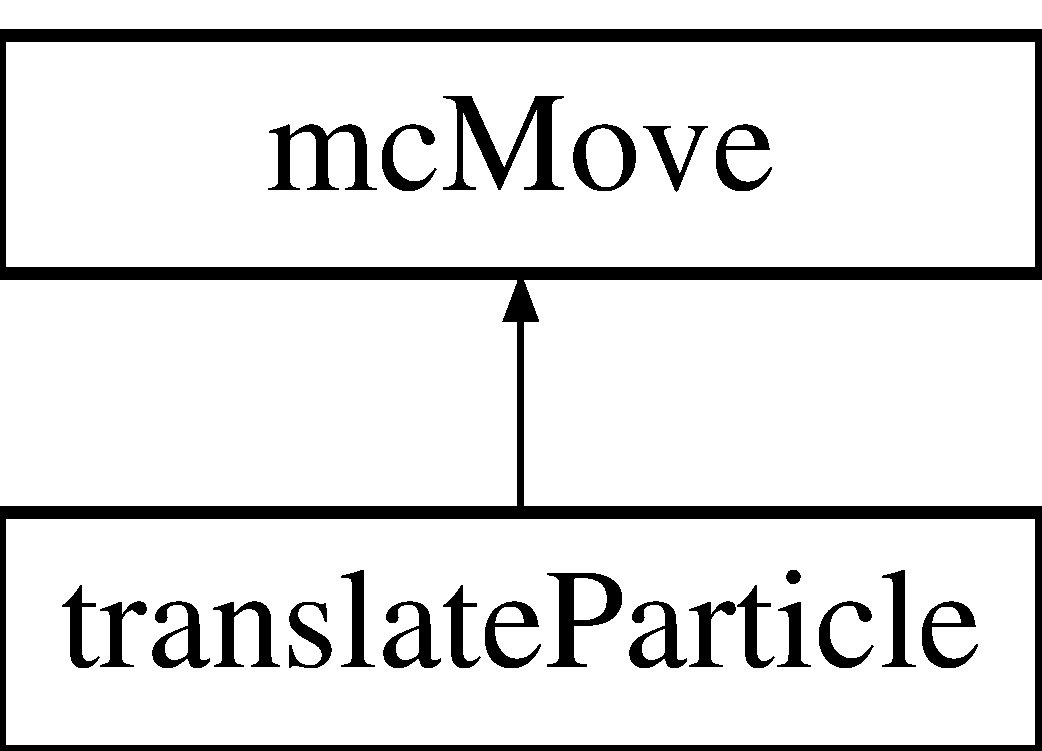
\includegraphics[height=2.000000cm]{classtranslate_particle}
\end{center}
\end{figure}
\subsection*{Public Member Functions}
\begin{DoxyCompactItemize}
\item 
\hyperlink{classtranslate_particle_ac16b682a2119d7ebd6c7df75fa224ab4}{translate\+Particle} ()
\item 
\hyperlink{classtranslate_particle_aa9ffcde3ec4cbd82e939c7cb9ee85094}{translate\+Particle} (const int type\+Index, const std\+::string tag)
\begin{DoxyCompactList}\small\item\em Instantiate a new move, also give a name which is the combination of auser-\/defined tag + the particle index it operates on. \end{DoxyCompactList}\item 
int \hyperlink{classtranslate_particle_a7ec5c9259f1aae3f7aefdb4db3ee5468}{make} (\hyperlink{classsim_system}{sim\+System} \&sys)
\begin{DoxyCompactList}\small\item\em Translate a particle in the system. \end{DoxyCompactList}\item 
void \hyperlink{classtranslate_particle_a65beec2511e79198e6241ad2bc18b02c}{set\+Max\+Displacement} (const double max\+D, const std\+::vector$<$ double $>$ \&box)
\begin{DoxyCompactList}\small\item\em Set the maximum displacement in any single move. \end{DoxyCompactList}\item 
const double \hyperlink{classtranslate_particle_a5f1e76a0e8f20978b1c1069f698f89e6}{get\+Max\+Displacement} ()
\begin{DoxyCompactList}\small\item\em Return the max displacement allowed in a single move. \end{DoxyCompactList}\end{DoxyCompactItemize}
\subsection*{Additional Inherited Members}


\subsection{Detailed Description}


Definition at line 12 of file translate.\+h.



\subsection{Constructor \& Destructor Documentation}
\hypertarget{classtranslate_particle_ac16b682a2119d7ebd6c7df75fa224ab4}{}\index{translate\+Particle@{translate\+Particle}!translate\+Particle@{translate\+Particle}}
\index{translate\+Particle@{translate\+Particle}!translate\+Particle@{translate\+Particle}}
\subsubsection[{translate\+Particle()}]{\setlength{\rightskip}{0pt plus 5cm}translate\+Particle\+::translate\+Particle (
\begin{DoxyParamCaption}
{}
\end{DoxyParamCaption}
)\hspace{0.3cm}{\ttfamily [inline]}}\label{classtranslate_particle_ac16b682a2119d7ebd6c7df75fa224ab4}


Definition at line 14 of file translate.\+h.


\begin{DoxyCode}
14 \{\};
\end{DoxyCode}
\hypertarget{classtranslate_particle_aa9ffcde3ec4cbd82e939c7cb9ee85094}{}\index{translate\+Particle@{translate\+Particle}!translate\+Particle@{translate\+Particle}}
\index{translate\+Particle@{translate\+Particle}!translate\+Particle@{translate\+Particle}}
\subsubsection[{translate\+Particle(const int type\+Index, const std\+::string tag)}]{\setlength{\rightskip}{0pt plus 5cm}translate\+Particle\+::translate\+Particle (
\begin{DoxyParamCaption}
\item[{const int}]{type\+Index, }
\item[{const std\+::string}]{tag}
\end{DoxyParamCaption}
)\hspace{0.3cm}{\ttfamily [inline]}}\label{classtranslate_particle_aa9ffcde3ec4cbd82e939c7cb9ee85094}


Instantiate a new move, also give a name which is the combination of auser-\/defined tag + the particle index it operates on. 



Definition at line 15 of file translate.\+h.



References mc\+Move\+::name\+\_\+, and mc\+Move\+::type\+Index\+\_\+.



\subsection{Member Function Documentation}
\hypertarget{classtranslate_particle_a5f1e76a0e8f20978b1c1069f698f89e6}{}\index{translate\+Particle@{translate\+Particle}!get\+Max\+Displacement@{get\+Max\+Displacement}}
\index{get\+Max\+Displacement@{get\+Max\+Displacement}!translate\+Particle@{translate\+Particle}}
\subsubsection[{get\+Max\+Displacement()}]{\setlength{\rightskip}{0pt plus 5cm}const double translate\+Particle\+::get\+Max\+Displacement (
\begin{DoxyParamCaption}
{}
\end{DoxyParamCaption}
)\hspace{0.3cm}{\ttfamily [inline]}}\label{classtranslate_particle_a5f1e76a0e8f20978b1c1069f698f89e6}


Return the max displacement allowed in a single move. 



Definition at line 18 of file translate.\+h.

\hypertarget{classtranslate_particle_a7ec5c9259f1aae3f7aefdb4db3ee5468}{}\index{translate\+Particle@{translate\+Particle}!make@{make}}
\index{make@{make}!translate\+Particle@{translate\+Particle}}
\subsubsection[{make(sim\+System \&sys)}]{\setlength{\rightskip}{0pt plus 5cm}int translate\+Particle\+::make (
\begin{DoxyParamCaption}
\item[{{\bf sim\+System} \&}]{sys}
\end{DoxyParamCaption}
)\hspace{0.3cm}{\ttfamily [virtual]}}\label{classtranslate_particle_a7ec5c9259f1aae3f7aefdb4db3ee5468}


Translate a particle in the system. 

All other information is stored in the \hyperlink{classsim_system}{sim\+System} object.


\begin{DoxyParams}[1]{Parameters}
\mbox{\tt in}  & {\em sys} & System object to attempt to remove a particle from.\\
\hline
\end{DoxyParams}
\begin{DoxyReturn}{Returns}
M\+O\+V\+E\+\_\+\+S\+U\+C\+C\+E\+S\+S if translated a particle, otherwise M\+O\+V\+E\+\_\+\+F\+A\+I\+L\+U\+R\+E if did not. Will throw exceptions if there was an error. 
\end{DoxyReturn}


Implements \hyperlink{classmc_move_a2e377a628f9ecee5422fc8967d4924eb}{mc\+Move}.



Definition at line 10 of file translate.\+cpp.



References sim\+System\+::atoms, sim\+System\+::beta(), sim\+System\+::box(), calculate\+Bias(), sim\+System\+::get\+Neighbor\+Positions(), sim\+System\+::get\+Tot\+N(), sim\+System\+::get\+W\+A\+L\+A\+Bias(), sim\+System\+::increment\+Energy(), M\+O\+V\+E\+\_\+\+F\+A\+I\+L\+U\+R\+E, M\+O\+V\+E\+\_\+\+S\+U\+C\+C\+E\+S\+S, sim\+System\+::n\+Species(), sim\+System\+::num\+Species, sim\+System\+::ppot, rng(), R\+N\+G\+\_\+\+S\+E\+E\+D, sim\+System\+::translate\+Atom(), mc\+Move\+::type\+Index\+\_\+, wala\+::update(), sim\+System\+::use\+W\+A\+L\+A, and custom\+Exception\+::what().


\begin{DoxyCode}
10                                            \{
11                 \textcolor{comment}{// check if any exist to be translated}
12     \textcolor{keywordflow}{if} (sys.\hyperlink{classsim_system_a9eea865e6dc1cff377b1e79c4d9c23f0}{numSpecies}[\hyperlink{classmc_move_acb731965547b0326ef318ec96da8b46a}{typeIndex\_}] < 1) \{
13         \textcolor{keywordflow}{return} \hyperlink{moves_8h_a9832cf5fcfa8c0894545b591c9908e39}{MOVE\_FAILURE};
14     \}
15     
16                 \textcolor{comment}{// choose a random particle of that type}
17                 \textcolor{keyword}{const} \textcolor{keywordtype}{int} chosenAtom = (int) floor(\hyperlink{utilities_8cpp_a0f9542af4b475ac79cb679d7a8d14db0}{rng} (&\hyperlink{global_8h_a3f4e4ea24d5a5c66feae55d1f329c884}{RNG\_SEED}) * sys.
      \hyperlink{classsim_system_a9eea865e6dc1cff377b1e79c4d9c23f0}{numSpecies}[\hyperlink{classmc_move_acb731965547b0326ef318ec96da8b46a}{typeIndex\_}]);
18  
19                 \textcolor{comment}{// attempt to translate that one}
20                 \textcolor{keyword}{const} std::vector < double > box = sys.\hyperlink{classsim_system_a8bff9dfb95b1b09a0fab2c1c485ade07}{box}();
21     \textcolor{keywordtype}{double} V = 1.0;
22     \textcolor{keywordflow}{for} (\textcolor{keywordtype}{unsigned} \textcolor{keywordtype}{int} i = 0; i < box.size(); ++i) \{
23         V *= box[i];
24     \}
25         
26     \textcolor{keywordtype}{double} oldEnergy = 0.0;
27     \textcolor{keywordflow}{for} (\textcolor{keywordtype}{unsigned} \textcolor{keywordtype}{int} spec = 0; spec < sys.\hyperlink{classsim_system_ab5e2e9b6204de15520302fe1d51688dd}{nSpecies}(); ++spec) \{
28         \textcolor{comment}{// get positions of neighboring atoms around chosenAtom}
29         std::vector< std::vector<double> > neighborPositions = sys.
      \hyperlink{classsim_system_a7ac49b2311cd8230df8d078a9d897b35}{getNeighborPositions}(spec, \hyperlink{classmc_move_acb731965547b0326ef318ec96da8b46a}{typeIndex\_}, &sys.\hyperlink{classsim_system_a90421b19082f7fb8fc23b7264b1161e4}{atoms}[
      \hyperlink{classmc_move_acb731965547b0326ef318ec96da8b46a}{typeIndex\_}][chosenAtom]);
30                 \textcolor{keywordflow}{for} (\textcolor{keywordtype}{unsigned} \textcolor{keywordtype}{int} i = 0; i < neighborPositions.size(); ++i) \{
31                                                 \textcolor{keywordflow}{try} \{
32                                                                 oldEnergy += sys.
      \hyperlink{classsim_system_a8d6271751a62f61edcf57f773540a4a3}{ppot}[spec][\hyperlink{classmc_move_acb731965547b0326ef318ec96da8b46a}{typeIndex\_}]->energy(neighborPositions[i], sys.\hyperlink{classsim_system_a90421b19082f7fb8fc23b7264b1161e4}{atoms}[
      \hyperlink{classmc_move_acb731965547b0326ef318ec96da8b46a}{typeIndex\_}][chosenAtom].pos, box);
33                                                 \}
34                                                 \textcolor{keywordflow}{catch} (\hyperlink{classcustom_exception}{customException}& ce) \{
35                                                                 std::string a = \textcolor{stringliteral}{"Cannot translate because
       of energy error: "}, b = ce.\hyperlink{classcustom_exception_aeb6ab5848b038adfc68fde86a512f691}{what}();
36                                                                 \textcolor{keywordflow}{throw} 
      \hyperlink{classcustom_exception}{customException} (a+b);
37                                                 \}
38         \}
39         \textcolor{comment}{// add tail correction to potential energy}
40 \textcolor{preprocessor}{#ifdef FLUID\_PHASE\_SIMULATIONS}
41         \textcolor{keywordflow}{if} (sys.\hyperlink{classsim_system_a8d6271751a62f61edcf57f773540a4a3}{ppot}[spec][\hyperlink{classmc_move_acb731965547b0326ef318ec96da8b46a}{typeIndex\_}]->useTailCorrection) \{
42                                                 oldEnergy += sys.\hyperlink{classsim_system_a8d6271751a62f61edcf57f773540a4a3}{ppot}[spec][
      \hyperlink{classmc_move_acb731965547b0326ef318ec96da8b46a}{typeIndex\_}]->tailCorrection((sys.\hyperlink{classsim_system_a9eea865e6dc1cff377b1e79c4d9c23f0}{numSpecies}[spec])/V);
43                                 \}
44 \textcolor{preprocessor}{#endif}
45     \}
46     
47     \textcolor{comment}{// store old position and move particle along random direction in interval [-maxD\_:maxD\_]}
48     std::vector<double> oldPos = sys.\hyperlink{classsim_system_a90421b19082f7fb8fc23b7264b1161e4}{atoms}[\hyperlink{classmc_move_acb731965547b0326ef318ec96da8b46a}{typeIndex\_}][chosenAtom].pos;
49     \textcolor{keywordflow}{for} (\textcolor{keywordtype}{unsigned} \textcolor{keywordtype}{int} i = 0; i< sys.\hyperlink{classsim_system_a90421b19082f7fb8fc23b7264b1161e4}{atoms}[\hyperlink{classmc_move_acb731965547b0326ef318ec96da8b46a}{typeIndex\_}][chosenAtom].pos.size(); ++i) \{
50                 sys.\hyperlink{classsim_system_a90421b19082f7fb8fc23b7264b1161e4}{atoms}[\hyperlink{classmc_move_acb731965547b0326ef318ec96da8b46a}{typeIndex\_}][chosenAtom].pos[i] += 2.0*maxD\_*(0.5-
      \hyperlink{utilities_8cpp_a0f9542af4b475ac79cb679d7a8d14db0}{rng} (&\hyperlink{global_8h_a3f4e4ea24d5a5c66feae55d1f329c884}{RNG\_SEED}));
51                 
52                 \textcolor{comment}{// apply periodic boundary conditions}
53                 \textcolor{keywordflow}{if} (sys.\hyperlink{classsim_system_a90421b19082f7fb8fc23b7264b1161e4}{atoms}[typeIndex\_][chosenAtom].pos[i] >= box[i]) \{
54                                 sys.\hyperlink{classsim_system_a90421b19082f7fb8fc23b7264b1161e4}{atoms}[\hyperlink{classmc_move_acb731965547b0326ef318ec96da8b46a}{typeIndex\_}][chosenAtom].pos[i] -= box[i];
55                 \} \textcolor{keywordflow}{else} \textcolor{keywordflow}{if} (sys.\hyperlink{classsim_system_a90421b19082f7fb8fc23b7264b1161e4}{atoms}[typeIndex\_][chosenAtom].pos[i] < 0) \{
56                                 sys.\hyperlink{classsim_system_a90421b19082f7fb8fc23b7264b1161e4}{atoms}[\hyperlink{classmc_move_acb731965547b0326ef318ec96da8b46a}{typeIndex\_}][chosenAtom].pos[i] += box[i];
57                 \}
58     \}
59     
60     \textcolor{comment}{// calculate energy at new position}
61     \textcolor{keywordtype}{double} newEnergy = 0.0;
62     \textcolor{keywordflow}{for} (\textcolor{keywordtype}{unsigned} \textcolor{keywordtype}{int} spec = 0; spec < sys.\hyperlink{classsim_system_ab5e2e9b6204de15520302fe1d51688dd}{nSpecies}(); ++spec) \{
63         \textcolor{comment}{// get positions of neighboring atoms around chosenAtom}
64         std::vector< std::vector<double> > neighborPositions = sys.
      \hyperlink{classsim_system_a7ac49b2311cd8230df8d078a9d897b35}{getNeighborPositions}(spec, typeIndex\_, &sys.\hyperlink{classsim_system_a90421b19082f7fb8fc23b7264b1161e4}{atoms}[typeIndex\_][chosenAtom]);
65                 \textcolor{keywordflow}{for} (\textcolor{keywordtype}{unsigned} \textcolor{keywordtype}{int} i = 0; i < neighborPositions.size(); ++i) \{
66                                                 \textcolor{keywordflow}{try} \{
67                                                                 newEnergy += sys.
      \hyperlink{classsim_system_a8d6271751a62f61edcf57f773540a4a3}{ppot}[spec][\hyperlink{classmc_move_acb731965547b0326ef318ec96da8b46a}{typeIndex\_}]->energy(neighborPositions[i], sys.\hyperlink{classsim_system_a90421b19082f7fb8fc23b7264b1161e4}{atoms}[typeIndex\_][chosenAtom].
      pos, box);
68                                                 \}
69                                                 \textcolor{keywordflow}{catch} (\hyperlink{classcustom_exception}{customException}& ce) \{
70                                                                 std::string a = \textcolor{stringliteral}{"Cannot delete because of
       energy error: "}, b = ce.\hyperlink{classcustom_exception_aeb6ab5848b038adfc68fde86a512f691}{what}();
71                                                                 \textcolor{keywordflow}{throw} 
      \hyperlink{classcustom_exception}{customException} (a+b);
72                                                 \}
73         \}
74         \textcolor{comment}{// add tail correction to potential energy}
75 \textcolor{preprocessor}{#ifdef FLUID\_PHASE\_SIMULATIONS}
76         \textcolor{keywordflow}{if} (sys.\hyperlink{classsim_system_a8d6271751a62f61edcf57f773540a4a3}{ppot}[spec][typeIndex\_]->useTailCorrection) \{
77                                                 newEnergy += sys.\hyperlink{classsim_system_a8d6271751a62f61edcf57f773540a4a3}{ppot}[spec][
      \hyperlink{classmc_move_acb731965547b0326ef318ec96da8b46a}{typeIndex\_}]->tailCorrection((sys.\hyperlink{classsim_system_a9eea865e6dc1cff377b1e79c4d9c23f0}{numSpecies}[spec])/V);
78                                 \}
79 \textcolor{preprocessor}{#endif}
80     \}
81     
82                 \textcolor{comment}{// biasing}
83                 \textcolor{keyword}{const} \textcolor{keywordtype}{double} p\_u = exp(-sys.\hyperlink{classsim_system_a3eeec9678902f8d7fce4dad6064aaf4c}{beta}()*(newEnergy - oldEnergy));
84                 \textcolor{keywordtype}{double} bias = \hyperlink{system_8cpp_ab912bbb9fc9045954cf1b3ccb286a55c}{calculateBias}(sys, sys.\hyperlink{classsim_system_a37dd827f4057049763351510147b9f1d}{getTotN}(), p\_u);
85                     
86                 \textcolor{keywordflow}{if} (\hyperlink{utilities_8cpp_a0f9542af4b475ac79cb679d7a8d14db0}{rng} (&\hyperlink{global_8h_a3f4e4ea24d5a5c66feae55d1f329c884}{RNG\_SEED}) < p\_u*bias) \{
87                     \textcolor{keywordflow}{try} \{
88             sys.\hyperlink{classsim_system_a22fdaceea44abd6cd021bac1ecd11890}{translateAtom}(typeIndex\_, chosenAtom, oldPos);
89         \} \textcolor{keywordflow}{catch} (\hyperlink{classcustom_exception}{customException} &ce) \{
90             std::string a = \textcolor{stringliteral}{"Failed to translate atom: "}, b = ce.\hyperlink{classcustom_exception_aeb6ab5848b038adfc68fde86a512f691}{what}();
91             \textcolor{keywordflow}{throw} \hyperlink{classcustom_exception}{customException} (a+b);
92         \}
93                                 sys.\hyperlink{classsim_system_a6ad31c08955b80873f865b3069618dcb}{incrementEnergy}(newEnergy - oldEnergy);      
94                                 
95                                 \textcolor{comment}{// update Wang-Landau bias, if used}
96                                 \textcolor{keywordflow}{if} (sys.\hyperlink{classsim_system_aa83b00006b3919fb6e13f1bdeadece6a}{useWALA}) \{
97                                                 sys.\hyperlink{classsim_system_a7cb5049de8b0988349e89e30e4000407}{getWALABias}()->
      \hyperlink{classwala_a5eb2622be6a9e89f5e59ba0b15aca4bd}{update}(sys.\hyperlink{classsim_system_a37dd827f4057049763351510147b9f1d}{getTotN}());
98                                 \}
99                                                 
100         \textcolor{keywordflow}{return} \hyperlink{moves_8h_ae8285cbddc5d21f73f49dcbad82a775a}{MOVE\_SUCCESS};
101     \}
102     
103     \textcolor{comment}{// if move failed, reset position}
104     \textcolor{keywordflow}{for} (\textcolor{keywordtype}{unsigned} \textcolor{keywordtype}{int} i = 0; i < sys.\hyperlink{classsim_system_a90421b19082f7fb8fc23b7264b1161e4}{atoms}[\hyperlink{classmc_move_acb731965547b0326ef318ec96da8b46a}{typeIndex\_}][chosenAtom].pos.size(); ++i) \{
105                 sys.\hyperlink{classsim_system_a90421b19082f7fb8fc23b7264b1161e4}{atoms}[\hyperlink{classmc_move_acb731965547b0326ef318ec96da8b46a}{typeIndex\_}][chosenAtom].pos[i] = oldPos[i];
106     \}
107     
108     \textcolor{comment}{// update Wang-Landau bias (even if moved failed), if used}
109     \textcolor{keywordflow}{if} (sys.\hyperlink{classsim_system_aa83b00006b3919fb6e13f1bdeadece6a}{useWALA}) \{
110                                 sys.\hyperlink{classsim_system_a7cb5049de8b0988349e89e30e4000407}{getWALABias}()->\hyperlink{classwala_a5eb2622be6a9e89f5e59ba0b15aca4bd}{update}(sys.
      \hyperlink{classsim_system_a37dd827f4057049763351510147b9f1d}{getTotN}());
111     \}
112                 
113                 \textcolor{keywordflow}{return} \hyperlink{moves_8h_a9832cf5fcfa8c0894545b591c9908e39}{MOVE\_FAILURE};
114 \}
\end{DoxyCode}
\hypertarget{classtranslate_particle_a65beec2511e79198e6241ad2bc18b02c}{}\index{translate\+Particle@{translate\+Particle}!set\+Max\+Displacement@{set\+Max\+Displacement}}
\index{set\+Max\+Displacement@{set\+Max\+Displacement}!translate\+Particle@{translate\+Particle}}
\subsubsection[{set\+Max\+Displacement(const double max\+D, const std\+::vector$<$ double $>$ \&box)}]{\setlength{\rightskip}{0pt plus 5cm}void translate\+Particle\+::set\+Max\+Displacement (
\begin{DoxyParamCaption}
\item[{const double}]{max\+D, }
\item[{const std\+::vector$<$ double $>$ \&}]{box}
\end{DoxyParamCaption}
)}\label{classtranslate_particle_a65beec2511e79198e6241ad2bc18b02c}


Set the maximum displacement in any single move. 

Should be postive number lss than half the box size.


\begin{DoxyParams}[1]{Parameters}
\mbox{\tt in}  & {\em max\+D} & Maximium displacement \\
\hline
\mbox{\tt in}  & {\em box} & Box dimensions \\
\hline
\end{DoxyParams}


Definition at line 122 of file translate.\+cpp.


\begin{DoxyCode}
122                                                                                               \{
123                 \textcolor{keywordflow}{for} (\textcolor{keywordtype}{unsigned} \textcolor{keywordtype}{int} i = 0; i < box.size(); ++i) \{
124                                 \textcolor{keywordflow}{if} (maxD >= box[i]/2.) \{
125                                                 \textcolor{keywordflow}{throw} \hyperlink{classcustom_exception}{customException} (\textcolor{stringliteral}{"Max displacement too
       large"});
126                                 \}
127                 \}
128                 \textcolor{keywordflow}{if} (maxD > 0) \{
129                                 maxD\_ = maxD;
130                 \} \textcolor{keywordflow}{else} \{
131                                 \textcolor{keywordflow}{throw} \hyperlink{classcustom_exception}{customException} (\textcolor{stringliteral}{"Max displacement must be positive"});
132                 \}
133 \}\end{DoxyCode}


The documentation for this class was generated from the following files\+:\begin{DoxyCompactItemize}
\item 
/\+Users/nam4/\+Desktop/omcs/src/\hyperlink{translate_8h}{translate.\+h}\item 
/\+Users/nam4/\+Desktop/omcs/src/\hyperlink{translate_8cpp}{translate.\+cpp}\end{DoxyCompactItemize}

\hypertarget{classwala}{}\section{wala Class Reference}
\label{classwala}\index{wala@{wala}}


Wang-\/\+Landau biasing class.  




{\ttfamily \#include $<$bias.\+h$>$}

\subsection*{Public Member Functions}
\begin{DoxyCompactItemize}
\item 
\hyperlink{classwala_a1a4483327eb3527ecc114c075b0b0598}{wala} ()
\item 
\hyperlink{classwala_a6f8890a10284e1551b1603ecc45433e8}{wala} (const double \hyperlink{classwala_acb8e59580d97bc3c5b9b4ff45eb6bb9a}{ln\+F}, const double g, const double s, const int Nmax, const int Nmin)
\begin{DoxyCompactList}\small\item\em Wang-\/\+Landau biasing constructor. \end{DoxyCompactList}\item 
void \hyperlink{classwala_a5eb2622be6a9e89f5e59ba0b15aca4bd}{update} (const int Nval)
\begin{DoxyCompactList}\small\item\em Update the estimate of the macrostate distribution. \end{DoxyCompactList}\item 
void \hyperlink{classwala_ae06c2f1475702ec9d1b0a243b7f34e4b}{iterate\+Forward} ()
\begin{DoxyCompactList}\small\item\em This should only be called when the \char`\"{}flatness\char`\"{} criterion is met. \end{DoxyCompactList}\item 
void \hyperlink{classwala_a65569289fac85d0da9c336e17c9d809a}{print} (const std\+::string file\+Name, const bool print\+H=false)
\begin{DoxyCompactList}\small\item\em Print the U\+N-\/\+N\+O\+R\+M\+A\+L\+I\+Z\+E\+D biasing function (ln\+P\+I) and possible the visted-\/states histogram to files. \end{DoxyCompactList}\item 
void \hyperlink{classwala_ae04916f49c11b0636e813787a3906570}{readln\+P\+I} (const std\+::string file\+Name)
\begin{DoxyCompactList}\small\item\em Read the macrostate distribution (biasing function) from a file. \end{DoxyCompactList}\item 
bool \hyperlink{classwala_add6302db96fcc45811b2944de2936525}{evaluate\+Flatness} ()
\begin{DoxyCompactList}\small\item\em Evaluate if the visited states histogram is approxiamtely \char`\"{}flat\char`\"{}. \end{DoxyCompactList}\item 
const \hyperlink{bias_8h_a1ceb524363fcb94da0c64d297ea27438}{\+\_\+\+\_\+\+B\+I\+A\+S\+\_\+\+I\+N\+T\+\_\+\+T\+Y\+P\+E\+\_\+\+\_\+} \hyperlink{classwala_a01a9bf2af8eaf65c719745ad1b12d238}{get\+Address} (const int Nval)
\begin{DoxyCompactList}\small\item\em For multidimensional Wang-\/\+Landau biasing, get the 1\+D coordinate of the macrostate distribution estimate (bias) for multidimensional data. \end{DoxyCompactList}\item 
const double \hyperlink{classwala_acb8e59580d97bc3c5b9b4ff45eb6bb9a}{ln\+F} ()
\item 
const double \hyperlink{classwala_a03f7b333aa0a280e78060bd9af7ec318}{get\+Bias} (const int address)
\item 
const std\+::vector$<$ double $>$ \hyperlink{classwala_a80b00e34135eb6da4e81cd0935622fc5}{getln\+P\+I} ()
\begin{DoxyCompactList}\small\item\em Return the current estimate of the macrostate distribution. \end{DoxyCompactList}\end{DoxyCompactItemize}


\subsection{Detailed Description}
Wang-\/\+Landau biasing class. 

Definition at line 48 of file bias.\+h.



\subsection{Constructor \& Destructor Documentation}
\hypertarget{classwala_a1a4483327eb3527ecc114c075b0b0598}{}\index{wala@{wala}!wala@{wala}}
\index{wala@{wala}!wala@{wala}}
\subsubsection[{wala()}]{\setlength{\rightskip}{0pt plus 5cm}wala\+::wala (
\begin{DoxyParamCaption}
{}
\end{DoxyParamCaption}
)\hspace{0.3cm}{\ttfamily [inline]}}\label{classwala_a1a4483327eb3527ecc114c075b0b0598}


Definition at line 50 of file bias.\+h.


\begin{DoxyCode}
50 \{\};
\end{DoxyCode}
\hypertarget{classwala_a6f8890a10284e1551b1603ecc45433e8}{}\index{wala@{wala}!wala@{wala}}
\index{wala@{wala}!wala@{wala}}
\subsubsection[{wala(const double ln\+F, const double g, const double s, const int Nmax, const int Nmin)}]{\setlength{\rightskip}{0pt plus 5cm}wala\+::wala (
\begin{DoxyParamCaption}
\item[{const double}]{ln\+F, }
\item[{const double}]{g, }
\item[{const double}]{s, }
\item[{const int}]{Nmax, }
\item[{const int}]{Nmin}
\end{DoxyParamCaption}
)}\label{classwala_a6f8890a10284e1551b1603ecc45433e8}


Wang-\/\+Landau biasing constructor. 


\begin{DoxyParams}[1]{Parameters}
\mbox{\tt in}  & {\em ln\+F} & Factor by which the estimate of the density of states in updated each time it is visited. \\
\hline
\mbox{\tt in}  & {\em g} & Factor by which ln\+F is reduced (multiplied) once \char`\"{}flatness\char`\"{} has been achieved. \\
\hline
\mbox{\tt in}  & {\em s} & Factor by which the min(\+H) must be within the mean of H to be considered \char`\"{}flat\char`\"{}, e.\+g. 0.\+8 --$>$ min is within 20\% error of mean \\
\hline
\mbox{\tt in}  & {\em n\+Spec} & Number of species in the simulation. \\
\hline
\mbox{\tt in}  & {\em Nmax} & Upper bound for total number of particles. \\
\hline
\mbox{\tt in}  & {\em Nmin} & Lower bound for total number of particles. \\
\hline
\end{DoxyParams}


Definition at line 292 of file bias.\+cpp.



References \+\_\+\+\_\+\+B\+I\+A\+S\+\_\+\+I\+N\+T\+\_\+\+T\+Y\+P\+E\+\_\+\+\_\+, and ln\+F().


\begin{DoxyCode}
292                                                                                             \{
293                 \textcolor{keywordflow}{if} (\hyperlink{classwala_acb8e59580d97bc3c5b9b4ff45eb6bb9a}{lnF} < 0) \{
294                                 \textcolor{keywordflow}{throw} \hyperlink{classcustom_exception}{customException} (\textcolor{stringliteral}{"lnF in Wang-Landau cannot be < 0"});
295                 \}
296                 lnF\_ = \hyperlink{classwala_acb8e59580d97bc3c5b9b4ff45eb6bb9a}{lnF};
297                 
298                 \textcolor{keywordflow}{if} (g <= 0 || g >= 1) \{
299                                 \textcolor{keywordflow}{throw} \hyperlink{classcustom_exception}{customException} (\textcolor{stringliteral}{"In Wang-Landau 0 < g < 1"});
300                 \}
301                 g\_ = g;
302                 
303                 \textcolor{keywordflow}{if} (s <= 0 || s >= 1) \{
304                                 \textcolor{keywordflow}{throw} \hyperlink{classcustom_exception}{customException} (\textcolor{stringliteral}{"In Wang-Landau 0 < s < 1"});
305                 \}
306                 s\_ = s;
307                                 
308                 \textcolor{keywordflow}{if} (Nmin > Nmax) \{
309                                 \textcolor{keywordflow}{throw} \hyperlink{classcustom_exception}{customException} (\textcolor{stringliteral}{"Nmin > Nmax in Wang-Landau object"});
310                 \}
311                 
312                 \hyperlink{bias_8h_a1ceb524363fcb94da0c64d297ea27438}{\_\_BIAS\_INT\_TYPE\_\_} size = (Nmax - Nmin + 1);
313                 
314                 Nmin\_ = Nmin;
315                 Nmax\_ = Nmax;
316                 
317                 \textcolor{comment}{// attempt to allocate memory for macrostate distribution matrix and initializes it all to
       0}
318                 \textcolor{keywordflow}{try} \{
319                                 lnPI\_.resize(size, 0.0);
320                 \} \textcolor{keywordflow}{catch} (\textcolor{keyword}{const} std::bad\_alloc &ce) \{
321                                 \textcolor{keywordflow}{throw} \hyperlink{classcustom_exception}{customException} (\textcolor{stringliteral}{"Out of memory, cannot allocate space
       for macrostate distribution matrix in wala"});
322                 \}
323                 
324                 \textcolor{comment}{// initialize the visited-states histogram}
325                 \textcolor{keywordflow}{try} \{
326                                 H\_.resize(size, 0.0);
327                 \} \textcolor{keywordflow}{catch} (\textcolor{keyword}{const} std::bad\_alloc &ce) \{
328                                 \textcolor{keywordflow}{throw} \hyperlink{classcustom_exception}{customException} (\textcolor{stringliteral}{"Out of memory, cannot allocate space
       for visited-states histogram in wala"});
329                 \}
330 \}
\end{DoxyCode}


\subsection{Member Function Documentation}
\hypertarget{classwala_add6302db96fcc45811b2944de2936525}{}\index{wala@{wala}!evaluate\+Flatness@{evaluate\+Flatness}}
\index{evaluate\+Flatness@{evaluate\+Flatness}!wala@{wala}}
\subsubsection[{evaluate\+Flatness()}]{\setlength{\rightskip}{0pt plus 5cm}bool wala\+::evaluate\+Flatness (
\begin{DoxyParamCaption}
{}
\end{DoxyParamCaption}
)}\label{classwala_add6302db96fcc45811b2944de2936525}


Evaluate if the visited states histogram is approxiamtely \char`\"{}flat\char`\"{}. 

\begin{DoxyReturn}{Returns}
Returns whether the histogram is flat or not. 
\end{DoxyReturn}


Definition at line 358 of file bias.\+cpp.



References spec\+Exp.



Referenced by main().


\begin{DoxyCode}
358                              \{
359                 \textcolor{keywordtype}{double} min = H\_[0], lnMean = -DBL\_MAX;
360                 \textcolor{keywordflow}{for} (\textcolor{keywordtype}{unsigned} \textcolor{keywordtype}{int} i = 0; i < H\_.size(); ++i) \{
361                                 \textcolor{keywordflow}{if} (H\_[i] < min) \{
362                                                 min = H\_[i];
363                                 \}
364                                 
365                                 \textcolor{comment}{// summing so many doubles may overrun DBL\_MAX, so instead track the lnMean}
366                                 lnMean = \hyperlink{bias_8h_a9f1e113b6454173bd61677519ec34c3a}{specExp}(lnMean, log(H\_[i]));
367                 \}
368                 lnMean -= log(H\_.size());
369                 
370                 \textcolor{keywordflow}{if} (log(min) - lnMean > log(s\_)) \{
371                                 \textcolor{keywordflow}{return} \textcolor{keyword}{true};
372                 \}
373                 \textcolor{keywordflow}{return} \textcolor{keyword}{false};
374 \}
\end{DoxyCode}
\hypertarget{classwala_a01a9bf2af8eaf65c719745ad1b12d238}{}\index{wala@{wala}!get\+Address@{get\+Address}}
\index{get\+Address@{get\+Address}!wala@{wala}}
\subsubsection[{get\+Address(const int Nval)}]{\setlength{\rightskip}{0pt plus 5cm}const {\bf \+\_\+\+\_\+\+B\+I\+A\+S\+\_\+\+I\+N\+T\+\_\+\+T\+Y\+P\+E\+\_\+\+\_\+} wala\+::get\+Address (
\begin{DoxyParamCaption}
\item[{const int}]{Nval}
\end{DoxyParamCaption}
)}\label{classwala_a01a9bf2af8eaf65c719745ad1b12d238}


For multidimensional Wang-\/\+Landau biasing, get the 1\+D coordinate of the macrostate distribution estimate (bias) for multidimensional data. 


\begin{DoxyParams}[1]{Parameters}
\mbox{\tt in}  & {\em Nval} & Total number of atoms in the system \\
\hline
\end{DoxyParams}


Definition at line 337 of file bias.\+cpp.



References \+\_\+\+\_\+\+B\+I\+A\+S\+\_\+\+I\+N\+T\+\_\+\+T\+Y\+P\+E\+\_\+\+\_\+.



Referenced by calculate\+Bias(), and update().


\begin{DoxyCode}
337                                                         \{
338                 \hyperlink{bias_8h_a1ceb524363fcb94da0c64d297ea27438}{\_\_BIAS\_INT\_TYPE\_\_} x = Nval - Nmin\_;
339                 \textcolor{keywordflow}{return} x;
340 \}
\end{DoxyCode}
\hypertarget{classwala_a03f7b333aa0a280e78060bd9af7ec318}{}\index{wala@{wala}!get\+Bias@{get\+Bias}}
\index{get\+Bias@{get\+Bias}!wala@{wala}}
\subsubsection[{get\+Bias(const int address)}]{\setlength{\rightskip}{0pt plus 5cm}const double wala\+::get\+Bias (
\begin{DoxyParamCaption}
\item[{const int}]{address}
\end{DoxyParamCaption}
)\hspace{0.3cm}{\ttfamily [inline]}}\label{classwala_a03f7b333aa0a280e78060bd9af7ec318}


Definition at line 60 of file bias.\+h.



Referenced by calculate\+Bias().


\begin{DoxyCode}
60 \{ \textcolor{keywordflow}{return} -lnPI\_[address]; \}
\end{DoxyCode}
\hypertarget{classwala_a80b00e34135eb6da4e81cd0935622fc5}{}\index{wala@{wala}!getln\+P\+I@{getln\+P\+I}}
\index{getln\+P\+I@{getln\+P\+I}!wala@{wala}}
\subsubsection[{getln\+P\+I()}]{\setlength{\rightskip}{0pt plus 5cm}const std\+::vector$<$double$>$ wala\+::getln\+P\+I (
\begin{DoxyParamCaption}
{}
\end{DoxyParamCaption}
)\hspace{0.3cm}{\ttfamily [inline]}}\label{classwala_a80b00e34135eb6da4e81cd0935622fc5}


Return the current estimate of the macrostate distribution. 



Definition at line 61 of file bias.\+h.



Referenced by main().

\hypertarget{classwala_ae06c2f1475702ec9d1b0a243b7f34e4b}{}\index{wala@{wala}!iterate\+Forward@{iterate\+Forward}}
\index{iterate\+Forward@{iterate\+Forward}!wala@{wala}}
\subsubsection[{iterate\+Forward()}]{\setlength{\rightskip}{0pt plus 5cm}void wala\+::iterate\+Forward (
\begin{DoxyParamCaption}
{}
\end{DoxyParamCaption}
)}\label{classwala_ae06c2f1475702ec9d1b0a243b7f34e4b}


This should only be called when the \char`\"{}flatness\char`\"{} criterion is met. 

This then resets the visited-\/states histogram H, and decrements ln\+F. 

Definition at line 379 of file bias.\+cpp.



Referenced by main().


\begin{DoxyCode}
379                            \{
380                 lnF\_ = lnF\_*g\_;
381                 std::fill(H\_.begin(), H\_.end(), 0);
382 \}
\end{DoxyCode}
\hypertarget{classwala_acb8e59580d97bc3c5b9b4ff45eb6bb9a}{}\index{wala@{wala}!ln\+F@{ln\+F}}
\index{ln\+F@{ln\+F}!wala@{wala}}
\subsubsection[{ln\+F()}]{\setlength{\rightskip}{0pt plus 5cm}const double wala\+::ln\+F (
\begin{DoxyParamCaption}
{}
\end{DoxyParamCaption}
)\hspace{0.3cm}{\ttfamily [inline]}}\label{classwala_acb8e59580d97bc3c5b9b4ff45eb6bb9a}


Definition at line 59 of file bias.\+h.



Referenced by main(), and wala().


\begin{DoxyCode}
59 \{ \textcolor{keywordflow}{return} lnF\_; \}
\end{DoxyCode}
\hypertarget{classwala_a65569289fac85d0da9c336e17c9d809a}{}\index{wala@{wala}!print@{print}}
\index{print@{print}!wala@{wala}}
\subsubsection[{print(const std\+::string file\+Name, const bool print\+H=false)}]{\setlength{\rightskip}{0pt plus 5cm}void wala\+::print (
\begin{DoxyParamCaption}
\item[{const std\+::string}]{file\+Name, }
\item[{const bool}]{print\+H = {\ttfamily false}}
\end{DoxyParamCaption}
)}\label{classwala_a65569289fac85d0da9c336e17c9d809a}


Print the U\+N-\/\+N\+O\+R\+M\+A\+L\+I\+Z\+E\+D biasing function (ln\+P\+I) and possible the visted-\/states histogram to files. 

Will overwrite the files if another with that name exists. Prints in net\+C\+D\+F format if enabled.


\begin{DoxyParams}[1]{Parameters}
\mbox{\tt in}  & {\em file\+Name} & Name of the file to print to. Will append with \char`\"{}\+\_\+ln\+P\+I\char`\"{} and \char`\"{}\+\_\+\+H\char`\"{} for the macrostate distribution and visited-\/states histogram, respectively. \\
\hline
\mbox{\tt in}  & {\em print\+H} & Defaults to false, but if true will also print the visited-\/states histogram. \\
\hline
\end{DoxyParams}


Definition at line 392 of file bias.\+cpp.



References sstr.



Referenced by main().


\begin{DoxyCode}
392                                                        \{
393 \textcolor{preprocessor}{#ifdef NETCDF\_CAPABLE}
394                 \textcolor{comment}{// Print visited-states histogram}
395                 \textcolor{keywordflow}{if} (printH) \{
396                                 \textcolor{keyword}{const} std::string name = fileName + \textcolor{stringliteral}{"\_H.nc"}
397                                 NcFile outFile(name.c\_str(), NcFile::replace);
398                                 NcDim probDim = outFile.addDim(\textcolor{stringliteral}{"vectorized\_position"}, H\_.size());
399                                 NcVar probVar = outFile.addVar(\textcolor{stringliteral}{"H"}, ncDouble, probDim);
400                                 \textcolor{keyword}{const} std::string dummyName = \textcolor{stringliteral}{"number\_species:"};
401                                 probVar.putAtt(dummyName.c\_str(), \hyperlink{utilities_8h_a8feb627efa8e8113cdf95f9a6151a088}{sstr}(nSpec\_).c\_str());
402                                 \textcolor{keyword}{const} std::string attName = \textcolor{stringliteral}{"species\_total\_upper\_bound:"};
403                                 probVar.putAtt(attName.c\_str(), \hyperlink{utilities_8h_a8feb627efa8e8113cdf95f9a6151a088}{sstr}(Nmax\_).c\_str());
404                                 \textcolor{keyword}{const} std::string attName = \textcolor{stringliteral}{"species\_upper\_lower\_bound:"};
405                                 probVar.putAtt(attName.c\_str(), \hyperlink{utilities_8h_a8feb627efa8e8113cdf95f9a6151a088}{sstr}(Nmin\_).c\_str());
406                                 probVar.putVar(&H\_[0]);
407                 \}
408                 
409                 \textcolor{comment}{// Print lnPI (bias) matrix}
410                 \textcolor{keyword}{const} std::string name = fileName + \textcolor{stringliteral}{"\_lnPI.nc"}
411                 NcFile outFile(name.c\_str(), NcFile::replace);
412                 NcDim probDim = outFile.addDim(\textcolor{stringliteral}{"vectorized\_position"}, lnPI\_.size());
413                 NcVar probVar = outFile.addVar(\textcolor{stringliteral}{"lnPI"}, ncDouble, probDim);
414                 \textcolor{keyword}{const} std::string dummyName = \textcolor{stringliteral}{"number\_species:"};
415                 probVar.putAtt(dummyName.c\_str(), \hyperlink{utilities_8h_a8feb627efa8e8113cdf95f9a6151a088}{sstr}(nSpec\_).c\_str());
416                 \textcolor{keyword}{const} std::string attName = \textcolor{stringliteral}{"species\_total\_upper\_bound:"};
417                 probVar.putAtt(attName.c\_str(), \hyperlink{utilities_8h_a8feb627efa8e8113cdf95f9a6151a088}{sstr}(Nmax\_).c\_str());
418                 \textcolor{keyword}{const} std::string attName = \textcolor{stringliteral}{"species\_total\_lower\_bound:"};
419                 probVar.putAtt(attName.c\_str(), \hyperlink{utilities_8h_a8feb627efa8e8113cdf95f9a6151a088}{sstr}(Nmin\_).c\_str());
420                 probVar.putVar(&lnPI\_[0]);
421 \textcolor{preprocessor}{#else}
422                 \textcolor{comment}{// Print visited-states histogram}
423                 \textcolor{keywordflow}{if} (printH) \{
424                                 std::ofstream of;
425                                 of.open(fileName+\textcolor{stringliteral}{"\_H.dat"}, std::ofstream::out);
426                                 of << \textcolor{stringliteral}{"# Visited-states histogram in single row (vectorized) notation."} << 
      std::endl;
427                                 of << \textcolor{stringliteral}{"# species\_total\_upper\_bound:"} << Nmax\_ << std::endl;
428                                 of << \textcolor{stringliteral}{"# species\_total\_lower\_bound:"} << Nmin\_ << std::endl;
429                                 \textcolor{keywordflow}{for} (\textcolor{keywordtype}{long} \textcolor{keywordtype}{long} \textcolor{keywordtype}{int} i = 0; i < H\_.size(); ++i) \{
430                                                 of << H\_[i] << std::endl;
431                                 \}
432                                 of.close();
433                 \}
434                 
435                 \textcolor{comment}{// Print lnPI (bias) matrix}
436                 std::ofstream of;
437                 of.open(fileName+\textcolor{stringliteral}{"\_lnPI.dat"}, std::ofstream::out);
438                 of << \textcolor{stringliteral}{"# lnPI (bias) matrix in single row (vectorized) notation."} << std::endl;
439                 of << \textcolor{stringliteral}{"# species\_total\_upper\_bound:"} << Nmax\_ << std::endl;
440                 of << \textcolor{stringliteral}{"# species\_total\_lower\_bound:"} << Nmin\_ << std::endl;
441                 \textcolor{keywordflow}{for} (\textcolor{keywordtype}{long} \textcolor{keywordtype}{long} \textcolor{keywordtype}{int} i = 0; i < lnPI\_.size(); ++i) \{
442                                 of << lnPI\_[i] << std::endl;
443                 \}
444                 of.close();
445 \textcolor{preprocessor}{#endif}
446 \}
\end{DoxyCode}
\hypertarget{classwala_ae04916f49c11b0636e813787a3906570}{}\index{wala@{wala}!readln\+P\+I@{readln\+P\+I}}
\index{readln\+P\+I@{readln\+P\+I}!wala@{wala}}
\subsubsection[{readln\+P\+I(const std\+::string file\+Name)}]{\setlength{\rightskip}{0pt plus 5cm}void wala\+::readln\+P\+I (
\begin{DoxyParamCaption}
\item[{const std\+::string}]{file\+Name}
\end{DoxyParamCaption}
)}\label{classwala_ae04916f49c11b0636e813787a3906570}


Read the macrostate distribution (biasing function) from a file. 

This assumes the user has already guaranteed that the bounds are consistent, e.\+g. Nmin and Nmax, as it will not check this automatically. Also assumes file was generated by this code. \char`\"{}\+Hand made\char`\"{} ones might have formatting issues since parsing is done based on tokens.


\begin{DoxyParams}[1]{Parameters}
\mbox{\tt in}  & {\em file\+Name} & Name of file containing ln\+P\+I. Must include file extension. \\
\hline
\end{DoxyParams}


Definition at line 455 of file bias.\+cpp.



References \+\_\+\+\_\+\+B\+I\+A\+S\+\_\+\+I\+N\+T\+\_\+\+T\+Y\+P\+E\+\_\+\+\_\+.


\begin{DoxyCode}
455                                              \{
456 \textcolor{preprocessor}{#ifdef NETCDF\_CAPABLE}
457                 NcFile dataFile (fileName.c\_str(), NcFile::read);
458                 NcVar lnPI\_data = dataFile.getVar(\textcolor{stringliteral}{"lnPI"});
459                 \textcolor{keywordflow}{if} (lnPI\_data.isNull()) \textcolor{keywordflow}{throw} \hyperlink{classcustom_exception}{customException}(\textcolor{stringliteral}{"Macrostate distribution
       matrix (biasing function) was empty, cannot read"});
460                 lnPI\_data.getVar(&lnPI\_[0]);
461 \textcolor{preprocessor}{#else}
462                 std::string line;
463                 std::ifstream inF (fileName);
464                 
465                 \textcolor{comment}{// Skip file header}
466                 \textcolor{keywordtype}{bool} header = \textcolor{keyword}{true};
467                 \textcolor{keywordflow}{while} (header) \{
468                                 std::getline (inF, line);
469                                 \textcolor{keywordflow}{if} (line.compare(0,1,\textcolor{stringliteral}{"#"},0,1) != 0) \{
470                                                 header = \textcolor{keyword}{false};
471                                 \}
472                 \}
473                 
474                 \textcolor{comment}{// Read line by line, parsing based on token}
475                 lnPI\_[0] = atof(line.c\_str());
476                 \hyperlink{bias_8h_a1ceb524363fcb94da0c64d297ea27438}{\_\_BIAS\_INT\_TYPE\_\_} index = 1;
477                 \textcolor{keywordflow}{while} (inF >> lnPI\_[index]) \{
478                                 index++;
479                 \}
480 \textcolor{preprocessor}{#endif}
481 \textcolor{preprocessor}{\}\end{DoxyCode}
\hypertarget{classwala_a5eb2622be6a9e89f5e59ba0b15aca4bd}{}\index{wala@{wala}!update@{update}}
\index{update@{update}!wala@{wala}}
\subsubsection[{update(const int Nval)}]{\setlength{\rightskip}{0pt plus 5cm}void wala\+::update (
\begin{DoxyParamCaption}
\item[{const int}]{Nval}
\end{DoxyParamCaption}
)}\label{classwala_a5eb2622be6a9e89f5e59ba0b15aca4bd}


Update the estimate of the macrostate distribution. 


\begin{DoxyParams}[1]{Parameters}
\mbox{\tt in}  & {\em Nval} & Total current number of atoms in the system \\
\hline
\end{DoxyParams}


Definition at line 347 of file bias.\+cpp.



References \+\_\+\+\_\+\+B\+I\+A\+S\+\_\+\+I\+N\+T\+\_\+\+T\+Y\+P\+E\+\_\+\+\_\+, and get\+Address().



Referenced by delete\+Particle\+::make(), translate\+Particle\+::make(), swap\+Particles\+::make(), and insert\+Particle\+::make().


\begin{DoxyCode}
347                                  \{
348                 \hyperlink{bias_8h_a1ceb524363fcb94da0c64d297ea27438}{\_\_BIAS\_INT\_TYPE\_\_} address = \hyperlink{classwala_a01a9bf2af8eaf65c719745ad1b12d238}{getAddress} (Nval);
349                 lnPI\_[address] += lnF\_;
350                 H\_[address] += 1.0;
351 \}
\end{DoxyCode}


The documentation for this class was generated from the following files\+:\begin{DoxyCompactItemize}
\item 
/\+Users/nam4/\+Desktop/omcs/src/\hyperlink{bias_8h}{bias.\+h}\item 
/\+Users/nam4/\+Desktop/omcs/src/\hyperlink{bias_8cpp}{bias.\+cpp}\end{DoxyCompactItemize}

\chapter{File Documentation}
\hypertarget{aggvolbias_8cpp}{\section{/home/nam4/\-Desktop/sandbox/\-F\-H\-M\-C\-Simulation/src/aggvolbias.cpp File Reference}
\label{aggvolbias_8cpp}\index{/home/nam4/\-Desktop/sandbox/\-F\-H\-M\-C\-Simulation/src/aggvolbias.\-cpp@{/home/nam4/\-Desktop/sandbox/\-F\-H\-M\-C\-Simulation/src/aggvolbias.\-cpp}}
}
{\ttfamily \#include \char`\"{}aggvolbias.\-h\char`\"{}}\\*

\hypertarget{aggvolbias_8h}{\section{/home/nam4/\-Desktop/sandbox/\-F\-H\-M\-C\-Simulation/src/aggvolbias.h File Reference}
\label{aggvolbias_8h}\index{/home/nam4/\-Desktop/sandbox/\-F\-H\-M\-C\-Simulation/src/aggvolbias.\-h@{/home/nam4/\-Desktop/sandbox/\-F\-H\-M\-C\-Simulation/src/aggvolbias.\-h}}
}
{\ttfamily \#include $<$cmath$>$}\\*
{\ttfamily \#include \char`\"{}system.\-h\char`\"{}}\\*
{\ttfamily \#include \char`\"{}global.\-h\char`\"{}}\\*
{\ttfamily \#include \char`\"{}moves.\-h\char`\"{}}\\*
{\ttfamily \#include \char`\"{}atom.\-h\char`\"{}}\\*
{\ttfamily \#include \char`\"{}utilities.\-h\char`\"{}}\\*
\subsection*{Data Structures}
\begin{DoxyCompactItemize}
\item 
class \hyperlink{classagg_vol_bias3}{agg\-Vol\-Bias3}
\item 
class \hyperlink{classagg_vol_bias_insert}{agg\-Vol\-Bias\-Insert}
\item 
class \hyperlink{classagg_vol_bias_delete}{agg\-Vol\-Bias\-Delete}
\end{DoxyCompactItemize}

\hypertarget{atom_8cpp}{\section{/home/nam4/\-Desktop/sandbox/\-F\-H\-M\-C\-Simulation/src/atom.cpp File Reference}
\label{atom_8cpp}\index{/home/nam4/\-Desktop/sandbox/\-F\-H\-M\-C\-Simulation/src/atom.\-cpp@{/home/nam4/\-Desktop/sandbox/\-F\-H\-M\-C\-Simulation/src/atom.\-cpp}}
}
{\ttfamily \#include \char`\"{}atom.\-h\char`\"{}}\\*
{\ttfamily \#include \char`\"{}utilities.\-h\char`\"{}}\\*

\hypertarget{atom_8h}{\section{/home/nam4/\-Desktop/sandbox/\-F\-H\-M\-C\-Simulation/src/atom.h File Reference}
\label{atom_8h}\index{/home/nam4/\-Desktop/sandbox/\-F\-H\-M\-C\-Simulation/src/atom.\-h@{/home/nam4/\-Desktop/sandbox/\-F\-H\-M\-C\-Simulation/src/atom.\-h}}
}
{\ttfamily \#include $<$vector$>$}\\*
{\ttfamily \#include \char`\"{}global.\-h\char`\"{}}\\*
{\ttfamily \#include \char`\"{}quaternion.\-h\char`\"{}}\\*
\subsection*{Data Structures}
\begin{DoxyCompactItemize}
\item 
class \hyperlink{classatom}{atom}
\begin{DoxyCompactList}\small\item\em Atom class with rigid internal degrees of freedom besides its center of mass. \end{DoxyCompactList}\end{DoxyCompactItemize}

\hypertarget{barrier_8cpp}{\section{/home/nam4/\-Desktop/sandbox/\-F\-H\-M\-C\-Simulation/src/barrier.cpp File Reference}
\label{barrier_8cpp}\index{/home/nam4/\-Desktop/sandbox/\-F\-H\-M\-C\-Simulation/src/barrier.\-cpp@{/home/nam4/\-Desktop/sandbox/\-F\-H\-M\-C\-Simulation/src/barrier.\-cpp}}
}
{\ttfamily \#include \char`\"{}barrier.\-h\char`\"{}}\\*

\hypertarget{barrier_8h}{\section{/home/nam4/\-Desktop/sandbox/\-F\-H\-M\-C\-Simulation/src/barrier.h File Reference}
\label{barrier_8h}\index{/home/nam4/\-Desktop/sandbox/\-F\-H\-M\-C\-Simulation/src/barrier.\-h@{/home/nam4/\-Desktop/sandbox/\-F\-H\-M\-C\-Simulation/src/barrier.\-h}}
}
{\ttfamily \#include $<$algorithm$>$}\\*
{\ttfamily \#include $<$cmath$>$}\\*
{\ttfamily \#include $<$vector$>$}\\*
{\ttfamily \#include $<$string$>$}\\*
{\ttfamily \#include \char`\"{}global.\-h\char`\"{}}\\*
{\ttfamily \#include \char`\"{}utilities.\-h\char`\"{}}\\*
{\ttfamily \#include \char`\"{}potentials.\-h\char`\"{}}\\*
{\ttfamily \#include \char`\"{}atom.\-h\char`\"{}}\\*
\subsection*{Data Structures}
\begin{DoxyCompactItemize}
\item 
class \hyperlink{classbarrier}{barrier}
\begin{DoxyCompactList}\small\item\em Virtual base class for barriers. \end{DoxyCompactList}\item 
class \hyperlink{classhard_wall_z}{hard\-Wall\-Z}
\begin{DoxyCompactList}\small\item\em Parallel hard walls in the z-\/direction. \end{DoxyCompactList}\item 
class \hyperlink{classsquare_well_wall_z}{square\-Well\-Wall\-Z}
\begin{DoxyCompactList}\small\item\em Parallel square-\/well walls in the z-\/direction. \end{DoxyCompactList}\item 
class \hyperlink{classcylinder_z}{cylinder\-Z}
\begin{DoxyCompactList}\small\item\em Cylinder along z = 0 axis at a given (x,y) coordinate. \end{DoxyCompactList}\item 
class \hyperlink{classright_triangle_x_z}{right\-Triangle\-X\-Z}
\item 
class \hyperlink{classcomposite_barrier}{composite\-Barrier}
\begin{DoxyCompactList}\small\item\em Class which tracks all barriers (superimposed) which interact with a given species. \end{DoxyCompactList}\end{DoxyCompactItemize}

\hypertarget{bias_8cpp}{\section{/home/nam4/\-Desktop/sandbox/\-F\-H\-M\-C\-Simulation/src/bias.cpp File Reference}
\label{bias_8cpp}\index{/home/nam4/\-Desktop/sandbox/\-F\-H\-M\-C\-Simulation/src/bias.\-cpp@{/home/nam4/\-Desktop/sandbox/\-F\-H\-M\-C\-Simulation/src/bias.\-cpp}}
}
{\ttfamily \#include \char`\"{}bias.\-h\char`\"{}}\\*

\hypertarget{bias_8h}{}\section{/\+Users/nam4/\+Desktop/omcs/src/bias.h File Reference}
\label{bias_8h}\index{/\+Users/nam4/\+Desktop/omcs/src/bias.\+h@{/\+Users/nam4/\+Desktop/omcs/src/bias.\+h}}
{\ttfamily \#include $<$vector$>$}\\*
{\ttfamily \#include $<$string$>$}\\*
{\ttfamily \#include $<$climits$>$}\\*
{\ttfamily \#include $<$cfloat$>$}\\*
{\ttfamily \#include $<$cmath$>$}\\*
{\ttfamily \#include $<$iostream$>$}\\*
{\ttfamily \#include $<$fstream$>$}\\*
{\ttfamily \#include \char`\"{}global.\+h\char`\"{}}\\*
{\ttfamily \#include \char`\"{}utilities.\+h\char`\"{}}\\*
\subsection*{Classes}
\begin{DoxyCompactItemize}
\item 
class \hyperlink{classtmmc}{tmmc}
\begin{DoxyCompactList}\small\item\em Transition Matrix Monte Carlo biasing class. \end{DoxyCompactList}\item 
class \hyperlink{classwala}{wala}
\begin{DoxyCompactList}\small\item\em Wang-\/\+Landau biasing class. \end{DoxyCompactList}\end{DoxyCompactItemize}
\subsection*{Macros}
\begin{DoxyCompactItemize}
\item 
\#define \hyperlink{bias_8h_a1ceb524363fcb94da0c64d297ea27438}{\+\_\+\+\_\+\+B\+I\+A\+S\+\_\+\+I\+N\+T\+\_\+\+T\+Y\+P\+E\+\_\+\+\_\+}~long long int
\begin{DoxyCompactList}\small\item\em For biasing, need to address things with large indices. \end{DoxyCompactList}\item 
\#define \hyperlink{bias_8h_a9f1e113b6454173bd61677519ec34c3a}{spec\+Exp}(a,  b)~std\+::max(a, b) + log(1.\+0 + exp(-\/std\+::abs(a-\/b)))
\begin{DoxyCompactList}\small\item\em Jacobi method for evaluating natural logarithm of a sum of exponentials E.\+g. \end{DoxyCompactList}\end{DoxyCompactItemize}


\subsection{Macro Definition Documentation}
\hypertarget{bias_8h_a1ceb524363fcb94da0c64d297ea27438}{}\index{bias.\+h@{bias.\+h}!\+\_\+\+\_\+\+B\+I\+A\+S\+\_\+\+I\+N\+T\+\_\+\+T\+Y\+P\+E\+\_\+\+\_\+@{\+\_\+\+\_\+\+B\+I\+A\+S\+\_\+\+I\+N\+T\+\_\+\+T\+Y\+P\+E\+\_\+\+\_\+}}
\index{\+\_\+\+\_\+\+B\+I\+A\+S\+\_\+\+I\+N\+T\+\_\+\+T\+Y\+P\+E\+\_\+\+\_\+@{\+\_\+\+\_\+\+B\+I\+A\+S\+\_\+\+I\+N\+T\+\_\+\+T\+Y\+P\+E\+\_\+\+\_\+}!bias.\+h@{bias.\+h}}
\subsubsection[{\+\_\+\+\_\+\+B\+I\+A\+S\+\_\+\+I\+N\+T\+\_\+\+T\+Y\+P\+E\+\_\+\+\_\+}]{\setlength{\rightskip}{0pt plus 5cm}\#define \+\_\+\+\_\+\+B\+I\+A\+S\+\_\+\+I\+N\+T\+\_\+\+T\+Y\+P\+E\+\_\+\+\_\+~long long int}\label{bias_8h_a1ceb524363fcb94da0c64d297ea27438}


For biasing, need to address things with large indices. 



Definition at line 15 of file bias.\+h.



Referenced by calculate\+Bias(), tmmc\+::calculate\+P\+I(), tmmc\+::check\+Fully\+Visited(), tmmc\+::get\+Address(), wala\+::get\+Address(), tmmc\+::get\+Transition\+Address(), tmmc\+::read\+C(), wala\+::readln\+P\+I(), tmmc\+::tmmc(), wala\+::update(), and wala\+::wala().

\hypertarget{bias_8h_a9f1e113b6454173bd61677519ec34c3a}{}\index{bias.\+h@{bias.\+h}!spec\+Exp@{spec\+Exp}}
\index{spec\+Exp@{spec\+Exp}!bias.\+h@{bias.\+h}}
\subsubsection[{spec\+Exp}]{\setlength{\rightskip}{0pt plus 5cm}\#define spec\+Exp(
\begin{DoxyParamCaption}
\item[{}]{a, }
\item[{}]{b}
\end{DoxyParamCaption}
)~std\+::max(a, b) + log(1.\+0 + exp(-\/std\+::abs(a-\/b)))}\label{bias_8h_a9f1e113b6454173bd61677519ec34c3a}


Jacobi method for evaluating natural logarithm of a sum of exponentials E.\+g. 

ln( exp(a) + exp(b) ) = \hyperlink{bias_8h_a9f1e113b6454173bd61677519ec34c3a}{spec\+Exp(a, b)} 

Definition at line 20 of file bias.\+h.



Referenced by wala\+::evaluate\+Flatness().


\hypertarget{cell_list_8cpp}{}\section{/\+Users/nam4/\+Desktop/omcs/src/cell\+List.cpp File Reference}
\label{cell_list_8cpp}\index{/\+Users/nam4/\+Desktop/omcs/src/cell\+List.\+cpp@{/\+Users/nam4/\+Desktop/omcs/src/cell\+List.\+cpp}}
{\ttfamily \#include \char`\"{}cell\+List.\+h\char`\"{}}\\*

\hypertarget{cell_list_8h}{\section{/home/nam4/\-Desktop/sandbox/\-F\-H\-M\-C\-Simulation/src/cell\-List.h File Reference}
\label{cell_list_8h}\index{/home/nam4/\-Desktop/sandbox/\-F\-H\-M\-C\-Simulation/src/cell\-List.\-h@{/home/nam4/\-Desktop/sandbox/\-F\-H\-M\-C\-Simulation/src/cell\-List.\-h}}
}
{\ttfamily \#include $<$iostream$>$}\\*
{\ttfamily \#include $<$fstream$>$}\\*
{\ttfamily \#include $<$cmath$>$}\\*
{\ttfamily \#include $<$vector$>$}\\*
{\ttfamily \#include $<$string$>$}\\*
{\ttfamily \#include \char`\"{}atom.\-h\char`\"{}}\\*
{\ttfamily \#include \char`\"{}global.\-h\char`\"{}}\\*
\subsection*{Data Structures}
\begin{DoxyCompactItemize}
\item 
class \hyperlink{classcell_list}{cell\-List}
\begin{DoxyCompactList}\small\item\em \hyperlink{classcell_list}{cell\-List} class. \end{DoxyCompactList}\end{DoxyCompactItemize}

\hypertarget{checkpoint_8cpp}{\section{/home/nam4/\-Desktop/sandbox/\-F\-H\-M\-C\-Simulation/src/checkpoint.cpp File Reference}
\label{checkpoint_8cpp}\index{/home/nam4/\-Desktop/sandbox/\-F\-H\-M\-C\-Simulation/src/checkpoint.\-cpp@{/home/nam4/\-Desktop/sandbox/\-F\-H\-M\-C\-Simulation/src/checkpoint.\-cpp}}
}
{\ttfamily \#include \char`\"{}checkpoint.\-h\char`\"{}}\\*

\hypertarget{checkpoint_8h}{\section{/home/nam4/\-Desktop/sandbox/\-F\-H\-M\-C\-Simulation/src/checkpoint.h File Reference}
\label{checkpoint_8h}\index{/home/nam4/\-Desktop/sandbox/\-F\-H\-M\-C\-Simulation/src/checkpoint.\-h@{/home/nam4/\-Desktop/sandbox/\-F\-H\-M\-C\-Simulation/src/checkpoint.\-h}}
}
{\ttfamily \#include $<$string$>$}\\*
{\ttfamily \#include $<$vector$>$}\\*
{\ttfamily \#include $<$ctime$>$}\\*
{\ttfamily \#include \char`\"{}global.\-h\char`\"{}}\\*
{\ttfamily \#include \char`\"{}system.\-h\char`\"{}}\\*
{\ttfamily \#include \char`\"{}utilities.\-h\char`\"{}}\\*
{\ttfamily \#include \char`\"{}rapidjson/include/rapidjson/document.\-h\char`\"{}}\\*
{\ttfamily \#include \char`\"{}rapidjson/include/rapidjson/writer.\-h\char`\"{}}\\*
{\ttfamily \#include \char`\"{}rapidjson/include/rapidjson/stringbuffer.\-h\char`\"{}}\\*
{\ttfamily \#include \char`\"{}rapidjson/include/rapidjson/filewritestream.\-h\char`\"{}}\\*
{\ttfamily \#include \char`\"{}rapidjson/include/rapidjson/filereadstream.\-h\char`\"{}}\\*
{\ttfamily \#include \char`\"{}rapidjson/include/rapidjson/prettywriter.\-h\char`\"{}}\\*
\subsection*{Data Structures}
\begin{DoxyCompactItemize}
\item 
class \hyperlink{classcheckpoint}{checkpoint}
\begin{DoxyCompactList}\small\item\em Information to restart/checkpoint the simulation. \end{DoxyCompactList}\end{DoxyCompactItemize}

\hypertarget{crossover_8cpp}{\section{/home/nam4/\-Desktop/sandbox/\-F\-H\-M\-C\-Simulation/src/crossover.cpp File Reference}
\label{crossover_8cpp}\index{/home/nam4/\-Desktop/sandbox/\-F\-H\-M\-C\-Simulation/src/crossover.\-cpp@{/home/nam4/\-Desktop/sandbox/\-F\-H\-M\-C\-Simulation/src/crossover.\-cpp}}
}
{\ttfamily \#include \char`\"{}crossover.\-h\char`\"{}}\\*
\subsection*{Functions}
\begin{DoxyCompactItemize}
\item 
void \hyperlink{crossover_8cpp_ac565cbacb4d42765f9cbe8da5f1f05ee}{perform\-Crossover} (\hyperlink{classsim_system}{sim\-System} \&sys, \hyperlink{classcheckpoint}{checkpoint} \&res, \hyperlink{classmoves}{moves} $\ast$used\-Moves\-Eq)
\begin{DoxyCompactList}\small\item\em Perform crossover from Wang-\/\-Landau stage of simulation to T\-M\-M\-C. \end{DoxyCompactList}\end{DoxyCompactItemize}


\subsection{Function Documentation}
\hypertarget{crossover_8cpp_ac565cbacb4d42765f9cbe8da5f1f05ee}{\index{crossover.\-cpp@{crossover.\-cpp}!perform\-Crossover@{perform\-Crossover}}
\index{perform\-Crossover@{perform\-Crossover}!crossover.cpp@{crossover.\-cpp}}
\subsubsection[{perform\-Crossover}]{\setlength{\rightskip}{0pt plus 5cm}void perform\-Crossover (
\begin{DoxyParamCaption}
\item[{{\bf sim\-System} \&}]{sys, }
\item[{{\bf checkpoint} \&}]{res, }
\item[{{\bf moves} $\ast$}]{used\-Moves\-Eq}
\end{DoxyParamCaption}
)}}\label{crossover_8cpp_ac565cbacb4d42765f9cbe8da5f1f05ee}


Perform crossover from Wang-\/\-Landau stage of simulation to T\-M\-M\-C. 


\begin{DoxyParams}[1]{Parameters}
\mbox{\tt in}  & {\em sys} & System to simulate \\
\hline
\mbox{\tt in}  & {\em res} & Restart/checkpoint information \\
\hline
\mbox{\tt in}  & {\em used\-Moves\-Eq} & Move class to use \\
\hline
\end{DoxyParams}


Definition at line 10 of file crossover.\-cpp.



References tmmc\-::calculate\-P\-I(), checkpoint\-::check(), sim\-System\-::check\-Energy\-Histogram\-Bounds(), tmmc\-::check\-Fully\-Visited(), checkpoint\-::crossover\-Done, sim\-System\-::crossover\-Total\-Step\-Counter, tmmc\-::dump\-Visited(), wala\-::evaluate\-Flatness(), sim\-System\-::get\-Current\-M(), sim\-System\-::get\-T\-M\-M\-C\-Bias(), sim\-System\-::get\-Total\-M(), sim\-System\-::get\-W\-A\-L\-A\-Bias(), tmmc\-::iterate\-Forward(), wala\-::iterate\-Forward(), wala\-::ln\-F(), moves\-::make\-Move(), checkpoint\-::move\-Counter, sim\-System\-::n\-Crossover\-Visits, tmmc\-::num\-Sweeps(), num\-To\-Str(), moves\-::print(), tmmc\-::print(), sim\-System\-::re\-Initialize\-Energy\-Histogram(), checkpoint\-::res\-From\-Cross, sanity\-Checks(), send\-Err(), send\-Msg(), sim\-System\-::start\-T\-M\-M\-C(), sim\-System\-::stop\-W\-A\-L\-A(), checkpoint\-::sweep\-Counter, S\-Y\-S\-\_\-\-F\-A\-I\-L\-U\-R\-E, sim\-System\-::tmmc\-Sweep\-Size, sim\-System\-::use\-W\-A\-L\-A, sim\-System\-::wala\-Total\-Step\-Counter, custom\-Exception\-::what(), and sim\-System\-::wl\-Sweep\-Size.


\begin{DoxyCode}
10                                                                             \{
11     \textcolor{keywordflow}{if} (res.\hyperlink{classcheckpoint_a4f13612ea6d376bb327295bfce3a70c5}{crossoverDone}) \{
12         \textcolor{keywordflow}{throw} \hyperlink{classcustom_exception}{customException} (\textcolor{stringliteral}{"Checkpoint indicates crossover already finished"});
13     \}
14     \hyperlink{utilities_8cpp_a08974c73a5b36c28b8ad1ef47fca77b0}{sendMsg}(\textcolor{stringliteral}{"Crossing over to build TMMC matrix"});
15 
16     res.\hyperlink{classcheckpoint_a4f13612ea6d376bb327295bfce3a70c5}{crossoverDone} = \textcolor{keyword}{false};
17     \textcolor{keywordtype}{long} \textcolor{keywordtype}{long} \textcolor{keywordtype}{int} timesFullyVisited = 0, moveStart = 0;
18     \textcolor{keywordflow}{if} (!res.\hyperlink{classcheckpoint_ac3e65d26f2b8231ae9dd7e29c72ecf3b}{resFromCross}) \{
19         \textcolor{keywordflow}{if} (!sys.\hyperlink{classsim_system_aa83b00006b3919fb6e13f1bdeadece6a}{useWALA}) \{
20             \textcolor{keywordflow}{throw} \hyperlink{classcustom_exception}{customException} (\textcolor{stringliteral}{"WALA not configured, cannot proceeed with crossover"});
21         \}
22         sys.\hyperlink{classsim_system_ac689245cd8e9ddfdcd94d3871a5a5d6b}{startTMMC} (sys.\hyperlink{classsim_system_a56e284a361964d0a9ce5c45f41d56ab1}{tmmcSweepSize}, sys.\hyperlink{classsim_system_aa4ad1afff101bb530e1590df05035276}{getTotalM}());
23     \} \textcolor{keywordflow}{else} \{
24         timesFullyVisited = res.\hyperlink{classcheckpoint_ad011ddbca1ea708321335b1b3ac67e07}{sweepCounter};
25         moveStart = res.\hyperlink{classcheckpoint_a5ab49a355714da4874aba00eb03f701d}{moveCounter};
26     \}
27 
28     \hyperlink{utilities_8cpp_a08974c73a5b36c28b8ad1ef47fca77b0}{sendMsg}(\textcolor{stringliteral}{"Starting from lnF = "}+\hyperlink{utilities_8h_ae6ed8fadf719af789711a7c0e99f44bc}{numToStr}(sys.\hyperlink{classsim_system_a7cb5049de8b0988349e89e30e4000407}{getWALABias}()->
      \hyperlink{classwala_acb8e59580d97bc3c5b9b4ff45eb6bb9a}{lnF}()));
29     \hyperlink{utilities_8cpp_a08974c73a5b36c28b8ad1ef47fca77b0}{sendMsg}(\textcolor{stringliteral}{"Starting from "}+\hyperlink{utilities_8h_ae6ed8fadf719af789711a7c0e99f44bc}{numToStr}(moveStart)+\textcolor{stringliteral}{" moves in current sweep"});
30     \hyperlink{utilities_8cpp_a08974c73a5b36c28b8ad1ef47fca77b0}{sendMsg}(\textcolor{stringliteral}{"Starting from "}+\hyperlink{utilities_8h_ae6ed8fadf719af789711a7c0e99f44bc}{numToStr}(timesFullyVisited)+\textcolor{stringliteral}{" out of "}+
      \hyperlink{utilities_8h_ae6ed8fadf719af789711a7c0e99f44bc}{numToStr}(sys.\hyperlink{classsim_system_aa748f651ddd9a2bf6d88bfcab9153905}{nCrossoverVisits})+\textcolor{stringliteral}{" sweeps"});
31 
32     \textcolor{keywordflow}{while} (timesFullyVisited < sys.\hyperlink{classsim_system_aa748f651ddd9a2bf6d88bfcab9153905}{nCrossoverVisits}) \{
33         \textcolor{keywordflow}{for} (\textcolor{keywordtype}{long} \textcolor{keywordtype}{long} \textcolor{keywordtype}{int} move = moveStart; move < sys.\hyperlink{classsim_system_ae625e1026daee4f99f83fb73881875a1}{wlSweepSize}; ++move) \{
34             \textcolor{keywordflow}{try} \{
35                 usedMovesEq->\hyperlink{classmoves_a7f023913b80bb62604b99f4dbf005c37}{makeMove}(sys);
36                 sys.\hyperlink{classsim_system_a1d71d1df76bba70136853e30823d2db9}{crossoverTotalStepCounter} += 1.0;
37             \} \textcolor{keywordflow}{catch} (\hyperlink{classcustom_exception}{customException} &ce) \{
38                 \hyperlink{utilities_8cpp_a6dacf3c3c19aa1e13a4d5a148fe5114e}{sendErr}(ce.\hyperlink{classcustom_exception_aeb6ab5848b038adfc68fde86a512f691}{what}());
39                 exit(\hyperlink{global_8h_a428dfe1ef0a6ff4b1fdebf275f6aff2e}{SYS\_FAILURE});
40             \}
41             \textcolor{keywordflow}{if} (sys.\hyperlink{classsim_system_a299fe4372e610b554eaaf5f5957b2dbc}{getCurrentM}() == 0) \{
42                 sys.\hyperlink{classsim_system_a176b9ff482f1d36bc0638538bcfe0670}{checkEnergyHistogramBounds} ();
43             \}
44             res.\hyperlink{classcheckpoint_a66cc1e90f61d47baafb9564c5c40ef9a}{check}(sys, move, timesFullyVisited, \textcolor{keyword}{false});
45         \}
46 
47         \textcolor{keywordflow}{if} (sys.\hyperlink{classsim_system_aa31d40c91cb50f143a9613d362798887}{getTMMCBias}()->\hyperlink{classtmmc_aa51f03f958dabefcff97be4a7c3b336c}{checkFullyVisited}()) \{
48             \textcolor{keywordflow}{try} \{
49                 sys.\hyperlink{classsim_system_aa31d40c91cb50f143a9613d362798887}{getTMMCBias}()->\hyperlink{classtmmc_a8e065523e9cc3c9628f91d3804cd201e}{calculatePI}();
50             \} \textcolor{keywordflow}{catch} (\hyperlink{classcustom_exception}{customException} &ce) \{
51                 \hyperlink{utilities_8cpp_a6dacf3c3c19aa1e13a4d5a148fe5114e}{sendErr}(ce.\hyperlink{classcustom_exception_aeb6ab5848b038adfc68fde86a512f691}{what}());
52                 sys.\hyperlink{classsim_system_aa31d40c91cb50f143a9613d362798887}{getTMMCBias}()->\hyperlink{classtmmc_ad49e147dc88b3e1c2975269598f94327}{print}(\textcolor{stringliteral}{"tmmc-crossover-fail"}, \textcolor{keyword}{true});
53                 sys.\hyperlink{classsim_system_aa31d40c91cb50f143a9613d362798887}{getTMMCBias}()->\hyperlink{classtmmc_a295886d2f7a947a9de890bcb3adb51c7}{dumpVisited}(\textcolor{stringliteral}{"tmmc-crossover-fail-visited"});
54                 exit(\hyperlink{global_8h_a428dfe1ef0a6ff4b1fdebf275f6aff2e}{SYS\_FAILURE});
55             \}
56             sys.\hyperlink{classsim_system_aa31d40c91cb50f143a9613d362798887}{getTMMCBias}()->\hyperlink{classtmmc_a611b5a86b3887afd9e90e2e4da66de35}{iterateForward} (); \textcolor{comment}{// Reset the counting matrix and
       increment total sweep number}
57             timesFullyVisited = sys.\hyperlink{classsim_system_aa31d40c91cb50f143a9613d362798887}{getTMMCBias}()->\hyperlink{classtmmc_afbdc037dc9b941d71d7049855e18f4be}{numSweeps}();
58             \hyperlink{utilities_8cpp_a08974c73a5b36c28b8ad1ef47fca77b0}{sendMsg}(\textcolor{stringliteral}{"Times C fully visited = "}+\hyperlink{utilities_8h_ae6ed8fadf719af789711a7c0e99f44bc}{numToStr}(timesFullyVisited));
59             usedMovesEq->\hyperlink{classmoves_acc6415d4000f01b93235d1a533aa6880}{print}(\textcolor{stringliteral}{"crossover.stats"});
60         \}
61 
62         \textcolor{comment}{// Check if bias has flattened out, just for continuous improvement}
63         \textcolor{keywordtype}{bool} flat = sys.\hyperlink{classsim_system_a7cb5049de8b0988349e89e30e4000407}{getWALABias}()->\hyperlink{classwala_add6302db96fcc45811b2944de2936525}{evaluateFlatness}();
64         \textcolor{keywordflow}{if} (flat) \{
65             sys.\hyperlink{classsim_system_a7cb5049de8b0988349e89e30e4000407}{getWALABias}()->\hyperlink{classwala_ae06c2f1475702ec9d1b0a243b7f34e4b}{iterateForward}(); \textcolor{comment}{// If flat, need to reset H and
       reduce lnF}
66             \hyperlink{utilities_8cpp_a08974c73a5b36c28b8ad1ef47fca77b0}{sendMsg}(\textcolor{stringliteral}{"Wang-Landau is now flat, new lnF = "}+\hyperlink{utilities_8h_ae6ed8fadf719af789711a7c0e99f44bc}{numToStr}(sys.
      \hyperlink{classsim_system_a7cb5049de8b0988349e89e30e4000407}{getWALABias}()->\hyperlink{classwala_acb8e59580d97bc3c5b9b4ff45eb6bb9a}{lnF}()));
67         \}
68     \}
69 
70     \textcolor{comment}{// Switch over to TMMC completely}
71     \hyperlink{utilities_8cpp_a08974c73a5b36c28b8ad1ef47fca77b0}{sendMsg}(\textcolor{stringliteral}{"Switching over to TMMC completely, ending Wang-Landau"});
72     sys.\hyperlink{classsim_system_ad6febde00f19ae0787771f2d1d9e391b}{stopWALA}();
73     \textcolor{keywordflow}{try} \{
74         sys.\hyperlink{classsim_system_aa31d40c91cb50f143a9613d362798887}{getTMMCBias}()->\hyperlink{classtmmc_a8e065523e9cc3c9628f91d3804cd201e}{calculatePI}();
75     \} \textcolor{keywordflow}{catch} (\hyperlink{classcustom_exception}{customException} &ce) \{
76         \hyperlink{utilities_8cpp_a6dacf3c3c19aa1e13a4d5a148fe5114e}{sendErr}(ce.\hyperlink{classcustom_exception_aeb6ab5848b038adfc68fde86a512f691}{what}());
77         sys.\hyperlink{classsim_system_aa31d40c91cb50f143a9613d362798887}{getTMMCBias}()->\hyperlink{classtmmc_ad49e147dc88b3e1c2975269598f94327}{print}(\textcolor{stringliteral}{"tmmc-beginning-fail"}, \textcolor{keyword}{true});
78         sys.\hyperlink{classsim_system_aa31d40c91cb50f143a9613d362798887}{getTMMCBias}()->\hyperlink{classtmmc_a295886d2f7a947a9de890bcb3adb51c7}{dumpVisited}(\textcolor{stringliteral}{"tmmc-beginning-fail-visited"});
79         exit(\hyperlink{global_8h_a428dfe1ef0a6ff4b1fdebf275f6aff2e}{SYS\_FAILURE});
80     \}
81 
82     sys.\hyperlink{classsim_system_a861dd81718ef1c069fa7cfb9b7efe83c}{reInitializeEnergyHistogram}(); \textcolor{comment}{// If doing initial WL "equilibration"
       re-initialize the histogram using bounds}
83     \hyperlink{sanity_8cpp_a73138cec3a48e4523004092dc0c2954b}{sanityChecks}(sys);
84     res.\hyperlink{classcheckpoint_a4f13612ea6d376bb327295bfce3a70c5}{crossoverDone} = \textcolor{keyword}{true}; \textcolor{comment}{// Do not need to dump a checkpoint}
85     \hyperlink{utilities_8cpp_a08974c73a5b36c28b8ad1ef47fca77b0}{sendMsg}(\textcolor{stringliteral}{"Completed "}+\hyperlink{utilities_8h_ae6ed8fadf719af789711a7c0e99f44bc}{numToStr}(sys.\hyperlink{classsim_system_a1d71d1df76bba70136853e30823d2db9}{crossoverTotalStepCounter})+\textcolor{stringliteral}{"
       total MC steps as part of crossover stage"});
86     \hyperlink{utilities_8cpp_a08974c73a5b36c28b8ad1ef47fca77b0}{sendMsg}(\textcolor{stringliteral}{"Total MC steps taken in simulation: "}+\hyperlink{utilities_8h_ae6ed8fadf719af789711a7c0e99f44bc}{numToStr}(sys.
      \hyperlink{classsim_system_a46f5d3a8843821b45fd3f4d9234a177f}{walaTotalStepCounter}+sys.\hyperlink{classsim_system_a1d71d1df76bba70136853e30823d2db9}{crossoverTotalStepCounter}));
87 \}
\end{DoxyCode}

\hypertarget{crossover_8h}{\section{/home/nam4/\-Desktop/sandbox/\-F\-H\-M\-C\-Simulation/src/crossover.h File Reference}
\label{crossover_8h}\index{/home/nam4/\-Desktop/sandbox/\-F\-H\-M\-C\-Simulation/src/crossover.\-h@{/home/nam4/\-Desktop/sandbox/\-F\-H\-M\-C\-Simulation/src/crossover.\-h}}
}
{\ttfamily \#include $<$string$>$}\\*
{\ttfamily \#include $<$memory$>$}\\*
{\ttfamily \#include \char`\"{}system.\-h\char`\"{}}\\*
{\ttfamily \#include \char`\"{}checkpoint.\-h\char`\"{}}\\*
{\ttfamily \#include \char`\"{}utilities.\-h\char`\"{}}\\*
{\ttfamily \#include \char`\"{}mover.\-h\char`\"{}}\\*
{\ttfamily \#include \char`\"{}sanity.\-h\char`\"{}}\\*
\subsection*{Functions}
\begin{DoxyCompactItemize}
\item 
void \hyperlink{crossover_8h_ac565cbacb4d42765f9cbe8da5f1f05ee}{perform\-Crossover} (\hyperlink{classsim_system}{sim\-System} \&sys, \hyperlink{classcheckpoint}{checkpoint} \&res, \hyperlink{classmoves}{moves} $\ast$used\-Moves\-Eq)
\begin{DoxyCompactList}\small\item\em Perform crossover from Wang-\/\-Landau stage of simulation to T\-M\-M\-C. \end{DoxyCompactList}\end{DoxyCompactItemize}


\subsection{Function Documentation}
\hypertarget{crossover_8h_ac565cbacb4d42765f9cbe8da5f1f05ee}{\index{crossover.\-h@{crossover.\-h}!perform\-Crossover@{perform\-Crossover}}
\index{perform\-Crossover@{perform\-Crossover}!crossover.h@{crossover.\-h}}
\subsubsection[{perform\-Crossover}]{\setlength{\rightskip}{0pt plus 5cm}void perform\-Crossover (
\begin{DoxyParamCaption}
\item[{{\bf sim\-System} \&}]{sys, }
\item[{{\bf checkpoint} \&}]{res, }
\item[{{\bf moves} $\ast$}]{used\-Moves\-Eq}
\end{DoxyParamCaption}
)}}\label{crossover_8h_ac565cbacb4d42765f9cbe8da5f1f05ee}


Perform crossover from Wang-\/\-Landau stage of simulation to T\-M\-M\-C. 


\begin{DoxyParams}[1]{Parameters}
\mbox{\tt in}  & {\em sys} & System to simulate \\
\hline
\mbox{\tt in}  & {\em res} & Restart/checkpoint information \\
\hline
\mbox{\tt in}  & {\em used\-Moves\-Eq} & Move class to use \\
\hline
\end{DoxyParams}


Definition at line 10 of file crossover.\-cpp.



References tmmc\-::calculate\-P\-I(), checkpoint\-::check(), sim\-System\-::check\-Energy\-Histogram\-Bounds(), tmmc\-::check\-Fully\-Visited(), checkpoint\-::crossover\-Done, tmmc\-::dump\-Visited(), wala\-::evaluate\-Flatness(), sim\-System\-::get\-Current\-M(), sim\-System\-::get\-T\-M\-M\-C\-Bias(), sim\-System\-::get\-Total\-M(), sim\-System\-::get\-W\-A\-L\-A\-Bias(), tmmc\-::iterate\-Forward(), wala\-::iterate\-Forward(), wala\-::ln\-F(), moves\-::make\-Move(), checkpoint\-::move\-Counter, sim\-System\-::n\-Crossover\-Visits, tmmc\-::num\-Sweeps(), num\-To\-Str(), moves\-::print(), tmmc\-::print(), sim\-System\-::re\-Initialize\-Energy\-Histogram(), checkpoint\-::res\-From\-Cross, sanity\-Checks(), send\-Err(), send\-Msg(), sim\-System\-::start\-T\-M\-M\-C(), sim\-System\-::stop\-W\-A\-L\-A(), checkpoint\-::sweep\-Counter, S\-Y\-S\-\_\-\-F\-A\-I\-L\-U\-R\-E, sim\-System\-::tmmc\-Sweep\-Size, sim\-System\-::use\-W\-A\-L\-A, custom\-Exception\-::what(), and sim\-System\-::wl\-Sweep\-Size.


\begin{DoxyCode}
10                                                                             \{
11     \textcolor{keywordflow}{if} (res.\hyperlink{classcheckpoint_a4f13612ea6d376bb327295bfce3a70c5}{crossoverDone}) \{
12         \textcolor{keywordflow}{throw} \hyperlink{classcustom_exception}{customException} (\textcolor{stringliteral}{"Checkpoint indicates crossover already finished"});
13     \}
14     \hyperlink{utilities_8cpp_a08974c73a5b36c28b8ad1ef47fca77b0}{sendMsg}(\textcolor{stringliteral}{"Crossing over to build TMMC matrix"});
15 
16     res.\hyperlink{classcheckpoint_a4f13612ea6d376bb327295bfce3a70c5}{crossoverDone} = \textcolor{keyword}{false};
17     \textcolor{keywordtype}{long} \textcolor{keywordtype}{long} \textcolor{keywordtype}{int} timesFullyVisited = 0, moveStart = 0;
18     \textcolor{keywordflow}{if} (!res.\hyperlink{classcheckpoint_ac3e65d26f2b8231ae9dd7e29c72ecf3b}{resFromCross}) \{
19         \textcolor{keywordflow}{if} (!sys.\hyperlink{classsim_system_aa83b00006b3919fb6e13f1bdeadece6a}{useWALA}) \{
20             \textcolor{keywordflow}{throw} \hyperlink{classcustom_exception}{customException} (\textcolor{stringliteral}{"WALA not configured, cannot proceeed with crossover"});
21         \}
22         sys.\hyperlink{classsim_system_ac689245cd8e9ddfdcd94d3871a5a5d6b}{startTMMC} (sys.\hyperlink{classsim_system_a56e284a361964d0a9ce5c45f41d56ab1}{tmmcSweepSize}, sys.\hyperlink{classsim_system_aa4ad1afff101bb530e1590df05035276}{getTotalM}());
23     \} \textcolor{keywordflow}{else} \{
24         timesFullyVisited = res.\hyperlink{classcheckpoint_ad011ddbca1ea708321335b1b3ac67e07}{sweepCounter};
25         moveStart = res.\hyperlink{classcheckpoint_a5ab49a355714da4874aba00eb03f701d}{moveCounter};
26     \}
27 
28     \hyperlink{utilities_8cpp_a08974c73a5b36c28b8ad1ef47fca77b0}{sendMsg}(\textcolor{stringliteral}{"Starting from lnF = "}+\hyperlink{utilities_8h_ae6ed8fadf719af789711a7c0e99f44bc}{numToStr}(sys.\hyperlink{classsim_system_a7cb5049de8b0988349e89e30e4000407}{getWALABias}()->
      \hyperlink{classwala_acb8e59580d97bc3c5b9b4ff45eb6bb9a}{lnF}()));
29     \hyperlink{utilities_8cpp_a08974c73a5b36c28b8ad1ef47fca77b0}{sendMsg}(\textcolor{stringliteral}{"Starting from "}+\hyperlink{utilities_8h_ae6ed8fadf719af789711a7c0e99f44bc}{numToStr}(moveStart)+\textcolor{stringliteral}{" moves in current sweep"});
30     \hyperlink{utilities_8cpp_a08974c73a5b36c28b8ad1ef47fca77b0}{sendMsg}(\textcolor{stringliteral}{"Starting from "}+\hyperlink{utilities_8h_ae6ed8fadf719af789711a7c0e99f44bc}{numToStr}(timesFullyVisited)+\textcolor{stringliteral}{" out of "}+
      \hyperlink{utilities_8h_ae6ed8fadf719af789711a7c0e99f44bc}{numToStr}(sys.\hyperlink{classsim_system_aa748f651ddd9a2bf6d88bfcab9153905}{nCrossoverVisits})+\textcolor{stringliteral}{" sweeps"});
31 
32     \textcolor{keywordflow}{while} (timesFullyVisited < sys.\hyperlink{classsim_system_aa748f651ddd9a2bf6d88bfcab9153905}{nCrossoverVisits}) \{
33         \textcolor{keywordflow}{for} (\textcolor{keywordtype}{long} \textcolor{keywordtype}{long} \textcolor{keywordtype}{int} move = moveStart; move < sys.\hyperlink{classsim_system_ae625e1026daee4f99f83fb73881875a1}{wlSweepSize}; ++move) \{
34             \textcolor{keywordflow}{try} \{
35                 usedMovesEq->\hyperlink{classmoves_a7f023913b80bb62604b99f4dbf005c37}{makeMove}(sys);
36             \} \textcolor{keywordflow}{catch} (\hyperlink{classcustom_exception}{customException} &ce) \{
37                 \hyperlink{utilities_8cpp_a6dacf3c3c19aa1e13a4d5a148fe5114e}{sendErr}(ce.\hyperlink{classcustom_exception_aeb6ab5848b038adfc68fde86a512f691}{what}());
38                 exit(\hyperlink{global_8h_a428dfe1ef0a6ff4b1fdebf275f6aff2e}{SYS\_FAILURE});
39             \}
40             \textcolor{keywordflow}{if} (sys.\hyperlink{classsim_system_a299fe4372e610b554eaaf5f5957b2dbc}{getCurrentM}() == 0) \{
41                 sys.\hyperlink{classsim_system_a176b9ff482f1d36bc0638538bcfe0670}{checkEnergyHistogramBounds} ();
42             \}
43             res.\hyperlink{classcheckpoint_ab2f76253fde665ee149c1380e78f5c2f}{check}(sys, move, timesFullyVisited);
44         \}
45 
46         \textcolor{keywordflow}{if} (sys.\hyperlink{classsim_system_aa31d40c91cb50f143a9613d362798887}{getTMMCBias}()->\hyperlink{classtmmc_aa51f03f958dabefcff97be4a7c3b336c}{checkFullyVisited}()) \{
47             \textcolor{keywordflow}{try} \{
48                 sys.\hyperlink{classsim_system_aa31d40c91cb50f143a9613d362798887}{getTMMCBias}()->\hyperlink{classtmmc_a8e065523e9cc3c9628f91d3804cd201e}{calculatePI}();
49             \} \textcolor{keywordflow}{catch} (\hyperlink{classcustom_exception}{customException} &ce) \{
50                 \hyperlink{utilities_8cpp_a6dacf3c3c19aa1e13a4d5a148fe5114e}{sendErr}(ce.\hyperlink{classcustom_exception_aeb6ab5848b038adfc68fde86a512f691}{what}());
51                 sys.\hyperlink{classsim_system_aa31d40c91cb50f143a9613d362798887}{getTMMCBias}()->\hyperlink{classtmmc_ad49e147dc88b3e1c2975269598f94327}{print}(\textcolor{stringliteral}{"tmmc-crossover-fail"}, \textcolor{keyword}{true});
52                 sys.\hyperlink{classsim_system_aa31d40c91cb50f143a9613d362798887}{getTMMCBias}()->\hyperlink{classtmmc_a295886d2f7a947a9de890bcb3adb51c7}{dumpVisited}(\textcolor{stringliteral}{"tmmc-crossover-fail-visited"});
53                 exit(\hyperlink{global_8h_a428dfe1ef0a6ff4b1fdebf275f6aff2e}{SYS\_FAILURE});
54             \}
55             sys.\hyperlink{classsim_system_aa31d40c91cb50f143a9613d362798887}{getTMMCBias}()->\hyperlink{classtmmc_a611b5a86b3887afd9e90e2e4da66de35}{iterateForward} (); \textcolor{comment}{// Reset the counting matrix and
       increment total sweep number}
56             timesFullyVisited = sys.\hyperlink{classsim_system_aa31d40c91cb50f143a9613d362798887}{getTMMCBias}()->\hyperlink{classtmmc_afbdc037dc9b941d71d7049855e18f4be}{numSweeps}();
57             \hyperlink{utilities_8cpp_a08974c73a5b36c28b8ad1ef47fca77b0}{sendMsg}(\textcolor{stringliteral}{"Times C fully visited = "}+\hyperlink{utilities_8h_ae6ed8fadf719af789711a7c0e99f44bc}{numToStr}(timesFullyVisited));
58             usedMovesEq->\hyperlink{classmoves_acc6415d4000f01b93235d1a533aa6880}{print}(\textcolor{stringliteral}{"crossover.stats"});
59         \}
60 
61         \textcolor{comment}{// Check if bias has flattened out, just for continuous improvement}
62         \textcolor{keywordtype}{bool} flat = sys.\hyperlink{classsim_system_a7cb5049de8b0988349e89e30e4000407}{getWALABias}()->\hyperlink{classwala_add6302db96fcc45811b2944de2936525}{evaluateFlatness}();
63         \textcolor{keywordflow}{if} (flat) \{
64             sys.\hyperlink{classsim_system_a7cb5049de8b0988349e89e30e4000407}{getWALABias}()->\hyperlink{classwala_ae06c2f1475702ec9d1b0a243b7f34e4b}{iterateForward}(); \textcolor{comment}{// If flat, need to reset H and
       reduce lnF}
65             \hyperlink{utilities_8cpp_a08974c73a5b36c28b8ad1ef47fca77b0}{sendMsg}(\textcolor{stringliteral}{"Wang-Landau is now flat, new lnF = "}+\hyperlink{utilities_8h_ae6ed8fadf719af789711a7c0e99f44bc}{numToStr}(sys.
      \hyperlink{classsim_system_a7cb5049de8b0988349e89e30e4000407}{getWALABias}()->\hyperlink{classwala_acb8e59580d97bc3c5b9b4ff45eb6bb9a}{lnF}()));
66         \}
67     \}
68 
69     \textcolor{comment}{// Switch over to TMMC completely}
70     \hyperlink{utilities_8cpp_a08974c73a5b36c28b8ad1ef47fca77b0}{sendMsg}(\textcolor{stringliteral}{"Switching over to TMMC completely, ending Wang-Landau"});
71     sys.\hyperlink{classsim_system_ad6febde00f19ae0787771f2d1d9e391b}{stopWALA}();
72     \textcolor{keywordflow}{try} \{
73         sys.\hyperlink{classsim_system_aa31d40c91cb50f143a9613d362798887}{getTMMCBias}()->\hyperlink{classtmmc_a8e065523e9cc3c9628f91d3804cd201e}{calculatePI}();
74     \} \textcolor{keywordflow}{catch} (\hyperlink{classcustom_exception}{customException} &ce) \{
75         \hyperlink{utilities_8cpp_a6dacf3c3c19aa1e13a4d5a148fe5114e}{sendErr}(ce.\hyperlink{classcustom_exception_aeb6ab5848b038adfc68fde86a512f691}{what}());
76         sys.\hyperlink{classsim_system_aa31d40c91cb50f143a9613d362798887}{getTMMCBias}()->\hyperlink{classtmmc_ad49e147dc88b3e1c2975269598f94327}{print}(\textcolor{stringliteral}{"tmmc-beginning-fail"}, \textcolor{keyword}{true});
77         sys.\hyperlink{classsim_system_aa31d40c91cb50f143a9613d362798887}{getTMMCBias}()->\hyperlink{classtmmc_a295886d2f7a947a9de890bcb3adb51c7}{dumpVisited}(\textcolor{stringliteral}{"tmmc-beginning-fail-visited"});
78         exit(\hyperlink{global_8h_a428dfe1ef0a6ff4b1fdebf275f6aff2e}{SYS\_FAILURE});
79     \}
80 
81     sys.\hyperlink{classsim_system_a861dd81718ef1c069fa7cfb9b7efe83c}{reInitializeEnergyHistogram}(); \textcolor{comment}{// If doing initial WL "equilibration"
       re-initialize the histogram using bounds}
82     \hyperlink{sanity_8cpp_a73138cec3a48e4523004092dc0c2954b}{sanityChecks}(sys);
83     res.\hyperlink{classcheckpoint_a4f13612ea6d376bb327295bfce3a70c5}{crossoverDone} = \textcolor{keyword}{true};
84 \}
\end{DoxyCode}

\hypertarget{delete_8cpp}{\section{/home/nam4/\-Desktop/sandbox/\-F\-H\-M\-C\-Simulation/src/delete.cpp File Reference}
\label{delete_8cpp}\index{/home/nam4/\-Desktop/sandbox/\-F\-H\-M\-C\-Simulation/src/delete.\-cpp@{/home/nam4/\-Desktop/sandbox/\-F\-H\-M\-C\-Simulation/src/delete.\-cpp}}
}
{\ttfamily \#include \char`\"{}delete.\-h\char`\"{}}\\*

\hypertarget{delete_8h}{}\section{/\+Users/nam4/\+Desktop/omcs/src/delete.h File Reference}
\label{delete_8h}\index{/\+Users/nam4/\+Desktop/omcs/src/delete.\+h@{/\+Users/nam4/\+Desktop/omcs/src/delete.\+h}}
{\ttfamily \#include $<$iostream$>$}\\*
{\ttfamily \#include $<$sstream$>$}\\*
{\ttfamily \#include $<$string$>$}\\*
{\ttfamily \#include \char`\"{}system.\+h\char`\"{}}\\*
{\ttfamily \#include \char`\"{}global.\+h\char`\"{}}\\*
{\ttfamily \#include \char`\"{}moves.\+h\char`\"{}}\\*
{\ttfamily \#include \char`\"{}atom.\+h\char`\"{}}\\*
\subsection*{Classes}
\begin{DoxyCompactItemize}
\item 
class \hyperlink{classdelete_particle}{delete\+Particle}
\end{DoxyCompactItemize}

\hypertarget{fhmc_8h}{\section{/home/nam4/\-Desktop/sandbox/\-F\-H\-M\-C\-Simulation/src/fhmc.h File Reference}
\label{fhmc_8h}\index{/home/nam4/\-Desktop/sandbox/\-F\-H\-M\-C\-Simulation/src/fhmc.\-h@{/home/nam4/\-Desktop/sandbox/\-F\-H\-M\-C\-Simulation/src/fhmc.\-h}}
}
{\ttfamily \#include $<$iostream$>$}\\*
{\ttfamily \#include \char`\"{}atom.\-h\char`\"{}}\\*
{\ttfamily \#include \char`\"{}barrier.\-h\char`\"{}}\\*
{\ttfamily \#include \char`\"{}bias.\-h\char`\"{}}\\*
{\ttfamily \#include \char`\"{}cell\-List.\-h\char`\"{}}\\*
{\ttfamily \#include \char`\"{}crossover.\-h\char`\"{}}\\*
{\ttfamily \#include \char`\"{}delete.\-h\char`\"{}}\\*
{\ttfamily \#include \char`\"{}gcmc.\-h\char`\"{}}\\*
{\ttfamily \#include \char`\"{}global.\-h\char`\"{}}\\*
{\ttfamily \#include \char`\"{}histogram.\-h\char`\"{}}\\*
{\ttfamily \#include \char`\"{}input.\-h\char`\"{}}\\*
{\ttfamily \#include \char`\"{}insert.\-h\char`\"{}}\\*
{\ttfamily \#include \char`\"{}mover.\-h\char`\"{}}\\*
{\ttfamily \#include \char`\"{}moves.\-h\char`\"{}}\\*
{\ttfamily \#include \char`\"{}potentials.\-h\char`\"{}}\\*
{\ttfamily \#include \char`\"{}quaternion.\-h\char`\"{}}\\*
{\ttfamily \#include \char`\"{}checkpoint.\-h\char`\"{}}\\*
{\ttfamily \#include \char`\"{}sanity.\-h\char`\"{}}\\*
{\ttfamily \#include \char`\"{}swap.\-h\char`\"{}}\\*
{\ttfamily \#include \char`\"{}system.\-h\char`\"{}}\\*
{\ttfamily \#include \char`\"{}tmmc.\-h\char`\"{}}\\*
{\ttfamily \#include \char`\"{}translate.\-h\char`\"{}}\\*
{\ttfamily \#include \char`\"{}utilities.\-h\char`\"{}}\\*
{\ttfamily \#include \char`\"{}wala.\-h\char`\"{}}\\*

\hypertarget{global_8h}{\section{/home/nam4/\-Desktop/sandbox/\-F\-H\-M\-C\-Simulation/src/global.h File Reference}
\label{global_8h}\index{/home/nam4/\-Desktop/sandbox/\-F\-H\-M\-C\-Simulation/src/global.\-h@{/home/nam4/\-Desktop/sandbox/\-F\-H\-M\-C\-Simulation/src/global.\-h}}
}
{\ttfamily \#include $<$string$>$}\\*
{\ttfamily \#include $<$exception$>$}\\*
\subsection*{Data Structures}
\begin{DoxyCompactItemize}
\item 
class \hyperlink{classcustom_exception}{custom\-Exception}
\begin{DoxyCompactList}\small\item\em Error handling via custom exceptions. \end{DoxyCompactList}\end{DoxyCompactItemize}
\subsection*{Macros}
\begin{DoxyCompactItemize}
\item 
\#define \hyperlink{global_8h_a428dfe1ef0a6ff4b1fdebf275f6aff2e}{S\-Y\-S\-\_\-\-F\-A\-I\-L\-U\-R\-E}~-\/1
\begin{DoxyCompactList}\small\item\em Returned from main the simualtion encountered a major error. \end{DoxyCompactList}\item 
\#define \hyperlink{global_8h_aee0da692ad91bbe61c65dc91c965b19d}{S\-A\-F\-E\-\_\-\-E\-X\-I\-T}~0
\begin{DoxyCompactList}\small\item\em Returned from main the simulation ran without error. \end{DoxyCompactList}\item 
\#define \hyperlink{global_8h_a598a3330b3c21701223ee0ca14316eca}{P\-I}~3.\-14159265359
\begin{DoxyCompactList}\small\item\em Numerical approximation of pi. \end{DoxyCompactList}\item 
\#define \hyperlink{global_8h_a85f9382b07ebd88cde9cd3667d50c0a6}{M\-A\-X\-\_\-\-B\-A\-R\-R\-I\-E\-R\-S\-\_\-\-P\-E\-R\-\_\-\-S\-P\-E\-C\-I\-E\-S}~100
\begin{DoxyCompactList}\small\item\em Max barrier number allowed for each species in input file. \end{DoxyCompactList}\item 
\#define \hyperlink{global_8h_af42f520b793f7c9dff15cba3bad0eb58}{H2\-\_\-2\-P\-I}~1.\-0
\begin{DoxyCompactList}\small\item\em Portion of de Broglie wavelength that is not mass or T-\/dependent, Delta = sqrt(H2\-\_\-2\-P\-I/mass/k\-T) \end{DoxyCompactList}\end{DoxyCompactItemize}
\subsection*{Variables}
\begin{DoxyCompactItemize}
\item 
int \hyperlink{global_8h_a3f4e4ea24d5a5c66feae55d1f329c884}{R\-N\-G\-\_\-\-S\-E\-E\-D}
\begin{DoxyCompactList}\small\item\em Default R\-N\-G seed. \end{DoxyCompactList}\end{DoxyCompactItemize}


\subsection{Macro Definition Documentation}
\hypertarget{global_8h_af42f520b793f7c9dff15cba3bad0eb58}{\index{global.\-h@{global.\-h}!H2\-\_\-2\-P\-I@{H2\-\_\-2\-P\-I}}
\index{H2\-\_\-2\-P\-I@{H2\-\_\-2\-P\-I}!global.h@{global.\-h}}
\subsubsection[{H2\-\_\-2\-P\-I}]{\setlength{\rightskip}{0pt plus 5cm}\#define H2\-\_\-2\-P\-I~1.\-0}}\label{global_8h_af42f520b793f7c9dff15cba3bad0eb58}


Portion of de Broglie wavelength that is not mass or T-\/dependent, Delta = sqrt(H2\-\_\-2\-P\-I/mass/k\-T) 



Definition at line 116 of file global.\-h.



Referenced by delete\-Particle\-::make(), and insert\-Particle\-::make().

\hypertarget{global_8h_a85f9382b07ebd88cde9cd3667d50c0a6}{\index{global.\-h@{global.\-h}!M\-A\-X\-\_\-\-B\-A\-R\-R\-I\-E\-R\-S\-\_\-\-P\-E\-R\-\_\-\-S\-P\-E\-C\-I\-E\-S@{M\-A\-X\-\_\-\-B\-A\-R\-R\-I\-E\-R\-S\-\_\-\-P\-E\-R\-\_\-\-S\-P\-E\-C\-I\-E\-S}}
\index{M\-A\-X\-\_\-\-B\-A\-R\-R\-I\-E\-R\-S\-\_\-\-P\-E\-R\-\_\-\-S\-P\-E\-C\-I\-E\-S@{M\-A\-X\-\_\-\-B\-A\-R\-R\-I\-E\-R\-S\-\_\-\-P\-E\-R\-\_\-\-S\-P\-E\-C\-I\-E\-S}!global.h@{global.\-h}}
\subsubsection[{M\-A\-X\-\_\-\-B\-A\-R\-R\-I\-E\-R\-S\-\_\-\-P\-E\-R\-\_\-\-S\-P\-E\-C\-I\-E\-S}]{\setlength{\rightskip}{0pt plus 5cm}\#define M\-A\-X\-\_\-\-B\-A\-R\-R\-I\-E\-R\-S\-\_\-\-P\-E\-R\-\_\-\-S\-P\-E\-C\-I\-E\-S~100}}\label{global_8h_a85f9382b07ebd88cde9cd3667d50c0a6}


Max barrier number allowed for each species in input file. 



Definition at line 115 of file global.\-h.



Referenced by set\-System\-Barriers().

\hypertarget{global_8h_a598a3330b3c21701223ee0ca14316eca}{\index{global.\-h@{global.\-h}!P\-I@{P\-I}}
\index{P\-I@{P\-I}!global.h@{global.\-h}}
\subsubsection[{P\-I}]{\setlength{\rightskip}{0pt plus 5cm}\#define P\-I~3.\-14159265359}}\label{global_8h_a598a3330b3c21701223ee0ca14316eca}


Numerical approximation of pi. 



Definition at line 114 of file global.\-h.



Referenced by agg\-Vol\-Bias3\-::make(), right\-Triangle\-X\-Z\-::right\-Triangle\-X\-Z(), quaternion\-::set\-Random\-Rot(), and lennard\-Jones\-::tail\-Correction().

\hypertarget{global_8h_aee0da692ad91bbe61c65dc91c965b19d}{\index{global.\-h@{global.\-h}!S\-A\-F\-E\-\_\-\-E\-X\-I\-T@{S\-A\-F\-E\-\_\-\-E\-X\-I\-T}}
\index{S\-A\-F\-E\-\_\-\-E\-X\-I\-T@{S\-A\-F\-E\-\_\-\-E\-X\-I\-T}!global.h@{global.\-h}}
\subsubsection[{S\-A\-F\-E\-\_\-\-E\-X\-I\-T}]{\setlength{\rightskip}{0pt plus 5cm}\#define S\-A\-F\-E\-\_\-\-E\-X\-I\-T~0}}\label{global_8h_aee0da692ad91bbe61c65dc91c965b19d}


Returned from main the simulation ran without error. 



Definition at line 113 of file global.\-h.

\hypertarget{global_8h_a428dfe1ef0a6ff4b1fdebf275f6aff2e}{\index{global.\-h@{global.\-h}!S\-Y\-S\-\_\-\-F\-A\-I\-L\-U\-R\-E@{S\-Y\-S\-\_\-\-F\-A\-I\-L\-U\-R\-E}}
\index{S\-Y\-S\-\_\-\-F\-A\-I\-L\-U\-R\-E@{S\-Y\-S\-\_\-\-F\-A\-I\-L\-U\-R\-E}!global.h@{global.\-h}}
\subsubsection[{S\-Y\-S\-\_\-\-F\-A\-I\-L\-U\-R\-E}]{\setlength{\rightskip}{0pt plus 5cm}\#define S\-Y\-S\-\_\-\-F\-A\-I\-L\-U\-R\-E~-\/1}}\label{global_8h_a428dfe1ef0a6ff4b1fdebf275f6aff2e}


Returned from main the simualtion encountered a major error. 



Definition at line 112 of file global.\-h.



Referenced by sim\-System\-::add\-Potential(), check\-Bounds(), initialize(), checkpoint\-::load(), moves\-::moves(), perform\-Crossover(), perform\-T\-M\-M\-C(), perform\-W\-A\-L\-A(), sim\-System\-::read\-Config(), sanity\-Checks(), set\-Config(), set\-Moves(), set\-Pair\-Potentials(), set\-System\-Barriers(), and sim\-System\-::sim\-System().



\subsection{Variable Documentation}
\hypertarget{global_8h_a3f4e4ea24d5a5c66feae55d1f329c884}{\index{global.\-h@{global.\-h}!R\-N\-G\-\_\-\-S\-E\-E\-D@{R\-N\-G\-\_\-\-S\-E\-E\-D}}
\index{R\-N\-G\-\_\-\-S\-E\-E\-D@{R\-N\-G\-\_\-\-S\-E\-E\-D}!global.h@{global.\-h}}
\subsubsection[{R\-N\-G\-\_\-\-S\-E\-E\-D}]{\setlength{\rightskip}{0pt plus 5cm}int R\-N\-G\-\_\-\-S\-E\-E\-D}}\label{global_8h_a3f4e4ea24d5a5c66feae55d1f329c884}


Default R\-N\-G seed. 



Definition at line 3 of file utilities.\-cpp.



Referenced by initialize(), agg\-Vol\-Bias3\-::make(), delete\-Particle\-::make(), translate\-Particle\-::make(), insert\-Particle\-::make(), swap\-Particles\-::make(), moves\-::make\-Move(), random3\-D\-Surface\-Vector(), and quaternion\-::set\-Random\-Rot().


\hypertarget{histogram_8cpp}{\section{/home/nam4/\-Desktop/sandbox/\-F\-H\-M\-C\-Simulation/src/histogram.cpp File Reference}
\label{histogram_8cpp}\index{/home/nam4/\-Desktop/sandbox/\-F\-H\-M\-C\-Simulation/src/histogram.\-cpp@{/home/nam4/\-Desktop/sandbox/\-F\-H\-M\-C\-Simulation/src/histogram.\-cpp}}
}
{\ttfamily \#include \char`\"{}histogram.\-h\char`\"{}}\\*
{\ttfamily \#include $<$iostream$>$}\\*

\hypertarget{histogram_8h}{\section{/home/nam4/\-Desktop/sandbox/\-F\-H\-M\-C\-Simulation/src/histogram.h File Reference}
\label{histogram_8h}\index{/home/nam4/\-Desktop/sandbox/\-F\-H\-M\-C\-Simulation/src/histogram.\-h@{/home/nam4/\-Desktop/sandbox/\-F\-H\-M\-C\-Simulation/src/histogram.\-h}}
}
{\ttfamily \#include $<$vector$>$}\\*
{\ttfamily \#include $<$deque$>$}\\*
{\ttfamily \#include $<$cmath$>$}\\*
{\ttfamily \#include $<$fstream$>$}\\*
{\ttfamily \#include $<$sstream$>$}\\*
{\ttfamily \#include $<$string$>$}\\*
{\ttfamily \#include \char`\"{}global.\-h\char`\"{}}\\*
{\ttfamily \#include \char`\"{}utilities.\-h\char`\"{}}\\*
\subsection*{Data Structures}
\begin{DoxyCompactItemize}
\item 
class \hyperlink{classhistogram}{histogram}
\item 
class \hyperlink{classdynamic__one__dim__histogram}{dynamic\-\_\-one\-\_\-dim\-\_\-histogram}
\end{DoxyCompactItemize}

\hypertarget{input_8cpp}{\section{/home/nam4/\-Desktop/sandbox/\-F\-H\-M\-C\-Simulation/src/input.cpp File Reference}
\label{input_8cpp}\index{/home/nam4/\-Desktop/sandbox/\-F\-H\-M\-C\-Simulation/src/input.\-cpp@{/home/nam4/\-Desktop/sandbox/\-F\-H\-M\-C\-Simulation/src/input.\-cpp}}
}
{\ttfamily \#include \char`\"{}input.\-h\char`\"{}}\\*
\subsection*{Functions}
\begin{DoxyCompactItemize}
\item 
void \hyperlink{input_8cpp_aa89df4b08049cfd9bdd875d78591ba5b}{check\-Bounds} (\hyperlink{classsim_system}{sim\-System} \&sys)
\begin{DoxyCompactList}\small\item\em Check the following bounds on system. \end{DoxyCompactList}\item 
\hyperlink{classsim_system}{sim\-System} \hyperlink{input_8cpp_a904001bba4e2facc93d1df9d214ed86e}{initialize} (const std\-::string filename, \hyperlink{classmoves}{moves} $\ast$used\-Moves\-Eq, \hyperlink{classmoves}{moves} $\ast$used\-Moves\-Pr)
\begin{DoxyCompactList}\small\item\em Parse a json input file and initialize system object accordingly. \end{DoxyCompactList}\item 
void \hyperlink{input_8cpp_a4541b66a5d6bfc7c4d90c3cf5c58ba27}{set\-Moves} (\hyperlink{classsim_system}{sim\-System} \&sys, const rapidjson\-::\-Document \&doc, \hyperlink{classmoves}{moves} $\ast$used\-Moves\-Eq, \hyperlink{classmoves}{moves} $\ast$used\-Moves\-Pr)
\begin{DoxyCompactList}\small\item\em Assign the Monte Carlo moves based on the J\-S\-O\-N input file. \end{DoxyCompactList}\item 
void \hyperlink{input_8cpp_afcd470506b012754a93b2012b65e3fc4}{set\-Pair\-Potentials} (\hyperlink{classsim_system}{sim\-System} \&sys, const rapidjson\-::\-Document \&doc)
\begin{DoxyCompactList}\small\item\em Assign the pair potentials based on the J\-S\-O\-N input file. \end{DoxyCompactList}\item 
void \hyperlink{input_8cpp_abb58279d5b9992aef3dcd304a3963954}{set\-Config} (\hyperlink{classsim_system}{sim\-System} \&sys, const std\-::string filename)
\begin{DoxyCompactList}\small\item\em Setup a system's initial configuration as necessary. \end{DoxyCompactList}\item 
void \hyperlink{input_8cpp_ab6dc74f7fbe4f517a72a21da3b795dfa}{set\-Barriers} (\hyperlink{classsim_system}{sim\-System} \&sys, const rapidjson\-::\-Document \&doc)
\begin{DoxyCompactList}\small\item\em Initialize the barriers in a system by parsing the input document. \end{DoxyCompactList}\end{DoxyCompactItemize}


\subsection{Function Documentation}
\hypertarget{input_8cpp_aa89df4b08049cfd9bdd875d78591ba5b}{\index{input.\-cpp@{input.\-cpp}!check\-Bounds@{check\-Bounds}}
\index{check\-Bounds@{check\-Bounds}!input.cpp@{input.\-cpp}}
\subsubsection[{check\-Bounds}]{\setlength{\rightskip}{0pt plus 5cm}void check\-Bounds (
\begin{DoxyParamCaption}
\item[{{\bf sim\-System} \&}]{sys}
\end{DoxyParamCaption}
)}}\label{input_8cpp_aa89df4b08049cfd9bdd875d78591ba5b}


Check the following bounds on system. 

If any fail, an emergency exit is performed.
\begin{DoxyEnumerate}
\item Check all pair potentials are set.
\item Check that rcut $<$ L/2 for all potentials
\end{DoxyEnumerate}


\begin{DoxyParams}[1]{Parameters}
\mbox{\tt in}  & {\em sys} & System to check bounds on \\
\hline
\end{DoxyParams}


Definition at line 10 of file input.\-cpp.



References sim\-System\-::box(), sim\-System\-::n\-Species(), num\-To\-Str(), sim\-System\-::potential\-Is\-Set(), sim\-System\-::ppot, send\-Err(), and S\-Y\-S\-\_\-\-F\-A\-I\-L\-U\-R\-E.



Referenced by initialize().


\begin{DoxyCode}
10                                   \{
11     \textcolor{comment}{// check all pair potentials have been set and all r\_cut < L/2}
12     \textcolor{keywordtype}{double} minL = sys.\hyperlink{classsim_system_a8bff9dfb95b1b09a0fab2c1c485ade07}{box}()[0];
13     \textcolor{keywordflow}{for} (\textcolor{keywordtype}{unsigned} \textcolor{keywordtype}{int} i = 1; i < 3; ++i) \{
14         minL = std::min(minL, sys.\hyperlink{classsim_system_a8bff9dfb95b1b09a0fab2c1c485ade07}{box}()[i]);
15     \}
16     \textcolor{keywordflow}{for} (\textcolor{keywordtype}{unsigned} \textcolor{keywordtype}{int} i = 0; i < sys.\hyperlink{classsim_system_ab5e2e9b6204de15520302fe1d51688dd}{nSpecies}(); ++i) \{
17         \textcolor{keywordflow}{for} (\textcolor{keywordtype}{unsigned} \textcolor{keywordtype}{int} j = 0; j < sys.\hyperlink{classsim_system_ab5e2e9b6204de15520302fe1d51688dd}{nSpecies}(); ++j) \{
18             \textcolor{keywordflow}{if} (!sys.\hyperlink{classsim_system_a40af191fae6091e26413ee06ae188ae9}{potentialIsSet}(i, j)) \{
19                 \hyperlink{utilities_8cpp_a6dacf3c3c19aa1e13a4d5a148fe5114e}{sendErr}(\textcolor{stringliteral}{"Not all pair potentials are set"});
20                 exit(\hyperlink{global_8h_a428dfe1ef0a6ff4b1fdebf275f6aff2e}{SYS\_FAILURE});
21             \}
22             \textcolor{keywordflow}{if} (!(sys.\hyperlink{classsim_system_ad2e290b5963f132e6a3a56cee35c8e9f}{ppot}[i][j]->rcut() < minL/2.0)) \{
23                 \hyperlink{utilities_8cpp_a6dacf3c3c19aa1e13a4d5a148fe5114e}{sendErr}(\textcolor{stringliteral}{"Pair potential r\_cut for species "}+\hyperlink{utilities_8h_ae6ed8fadf719af789711a7c0e99f44bc}{numToStr}(i)+\textcolor{stringliteral}{", "}+
      \hyperlink{utilities_8h_ae6ed8fadf719af789711a7c0e99f44bc}{numToStr}(j)+\textcolor{stringliteral}{" is > L/2"});
24                 exit(\hyperlink{global_8h_a428dfe1ef0a6ff4b1fdebf275f6aff2e}{SYS\_FAILURE});
25             \}
26         \}
27     \}
28 \}
\end{DoxyCode}
\hypertarget{input_8cpp_a904001bba4e2facc93d1df9d214ed86e}{\index{input.\-cpp@{input.\-cpp}!initialize@{initialize}}
\index{initialize@{initialize}!input.cpp@{input.\-cpp}}
\subsubsection[{initialize}]{\setlength{\rightskip}{0pt plus 5cm}{\bf sim\-System} initialize (
\begin{DoxyParamCaption}
\item[{const std\-::string}]{filename, }
\item[{{\bf moves} $\ast$}]{used\-Moves\-Eq, }
\item[{{\bf moves} $\ast$}]{used\-Moves\-Pr}
\end{DoxyParamCaption}
)}}\label{input_8cpp_a904001bba4e2facc93d1df9d214ed86e}


Parse a json input file and initialize system object accordingly. 

\mbox{[}in\mbox{]} filename Input J\-S\-O\-N document's filename  \mbox{[}in\mbox{]} used\-Moves\-Eq Pointer to move object that will be used during \char`\"{}equilibration\char`\"{} (W\-L)  \mbox{[}in\mbox{]} used\-Moves\-Pr Pointer to move object that will be used during \char`\"{}production\char`\"{} (T\-M\-M\-C) 

Definition at line 37 of file input.\-cpp.



References sim\-System\-::add\-K\-E\-Correction(), check\-Bounds(), sim\-System\-::ln\-F\-\_\-end, sim\-System\-::ln\-F\-\_\-start, sim\-System\-::n\-Crossover\-Visits, num\-To\-Str(), parse\-Json(), sim\-System\-::restart\-From\-T\-M\-M\-C, sim\-System\-::restart\-From\-T\-M\-M\-C\-File, sim\-System\-::restart\-From\-W\-A\-L\-A, sim\-System\-::restart\-From\-W\-A\-L\-A\-File, R\-N\-G\-\_\-\-S\-E\-E\-D, send\-Err(), send\-Msg(), set\-Barriers(), set\-Moves(), set\-Pair\-Potentials(), sim\-System\-::set\-Tot\-N\-Bounds(), S\-Y\-S\-\_\-\-F\-A\-I\-L\-U\-R\-E, sim\-System\-::tmmc\-Sweep\-Size, sim\-System\-::toggle\-K\-E(), sim\-System\-::total\-T\-M\-M\-C\-Sweeps, sim\-System\-::wala\-\_\-g, sim\-System\-::wala\-\_\-s, and sim\-System\-::wl\-Sweep\-Size.


\begin{DoxyCode}
37                                                                                         \{
38     rapidjson::Document doc;
39     \textcolor{keywordflow}{try} \{
40         \hyperlink{utilities_8cpp_a3f494918ff3c252de4914c9905be04e7}{parseJson} (filename, doc);
41     \} \textcolor{keywordflow}{catch} (std::exception &ex) \{
42         \textcolor{keywordflow}{throw} \hyperlink{classcustom_exception}{customException} (ex.what());
43     \}
44 
45     \textcolor{comment}{// Check each member exists and is in the correct format}
46     \textcolor{keywordflow}{if} (!doc.HasMember(\textcolor{stringliteral}{"num\_species"})) \textcolor{keywordflow}{throw} \hyperlink{classcustom_exception}{customException}(\textcolor{stringliteral}{"\(\backslash\)"num\_species\(\backslash\)" is not
       specified in "}+filename);
47     \textcolor{keywordflow}{if} (!doc[\textcolor{stringliteral}{"num\_species"}].IsInt()) \textcolor{keywordflow}{throw} \hyperlink{classcustom_exception}{customException}(\textcolor{stringliteral}{"\(\backslash\)"num\_species\(\backslash\)" is not an
       integer in "}+filename);
48 
49     \textcolor{keywordflow}{if} (!doc.HasMember(\textcolor{stringliteral}{"beta"})) \textcolor{keywordflow}{throw} \hyperlink{classcustom_exception}{customException}(\textcolor{stringliteral}{"\(\backslash\)"beta\(\backslash\)" is not specified in "}+
      filename);
50     \textcolor{keywordflow}{if} (!doc[\textcolor{stringliteral}{"beta"}].IsNumber()) \textcolor{keywordflow}{throw} \hyperlink{classcustom_exception}{customException}(\textcolor{stringliteral}{"\(\backslash\)"beta\(\backslash\)" is not a number in "}+
      filename);
51 
52     \textcolor{keywordflow}{if} (!doc.HasMember(\textcolor{stringliteral}{"box"})) \textcolor{keywordflow}{throw} \hyperlink{classcustom_exception}{customException}(\textcolor{stringliteral}{"\(\backslash\)"box\(\backslash\)" is not specified in "}+filename
      );
53     \textcolor{keywordflow}{if} (!doc[\textcolor{stringliteral}{"box"}].IsArray()) \textcolor{keywordflow}{throw} \hyperlink{classcustom_exception}{customException}(\textcolor{stringliteral}{"\(\backslash\)"box\(\backslash\)" is not an array in "}+filename)
      ;
54     \textcolor{keywordflow}{if} (doc[\textcolor{stringliteral}{"box"}].Size() != 3) \textcolor{keywordflow}{throw} \hyperlink{classcustom_exception}{customException}(\textcolor{stringliteral}{"\(\backslash\)"box\(\backslash\)" is not a length 3 array in "}+
      filename);
55     std::vector < double > sysBox (3, 0);
56     \textcolor{keywordflow}{for} (rapidjson::SizeType i = 0; i < doc[\textcolor{stringliteral}{"box"}].Size(); ++i) \{
57         \textcolor{keywordflow}{if} (!doc[\textcolor{stringliteral}{"box"}][i].IsNumber()) \textcolor{keywordflow}{throw} \hyperlink{classcustom_exception}{customException}(\textcolor{stringliteral}{"box index "}+
      \hyperlink{utilities_8h_ae6ed8fadf719af789711a7c0e99f44bc}{numToStr}(i)+\textcolor{stringliteral}{" is not a number in "}+filename);
58         sysBox[i] = doc[\textcolor{stringliteral}{"box"}][i].GetDouble();
59     \}
60 
61     \textcolor{keywordtype}{double} duh = 10.0;
62     \textcolor{keywordflow}{if} (doc.HasMember(\textcolor{stringliteral}{"delta\_u\_hist"})) \{
63         \textcolor{keywordflow}{if} (!doc[\textcolor{stringliteral}{"delta\_u\_hist"}].IsNumber()) \textcolor{keywordflow}{throw} \hyperlink{classcustom_exception}{customException}(\textcolor{stringliteral}{"\(\backslash\)"delta\_u\_hist\(\backslash\)" is not
       a number in "}+filename);
64         duh = doc[\textcolor{stringliteral}{"delta\_u\_hist"}].GetDouble();
65     \}
66 
67     \textcolor{keywordtype}{int} maxOrder = 2;
68     \textcolor{keywordflow}{if} (doc.HasMember(\textcolor{stringliteral}{"max\_order"})) \{
69         \textcolor{keywordflow}{if} (!doc[\textcolor{stringliteral}{"max\_order"}].IsInt()) \textcolor{keywordflow}{throw} \hyperlink{classcustom_exception}{customException}(\textcolor{stringliteral}{"\(\backslash\)"max\_order\(\backslash\)" is not an
       integer in "}+filename);
70         maxOrder = doc[\textcolor{stringliteral}{"max\_order"}].GetInt();
71     \}
72 
73     \textcolor{keywordtype}{bool} useKe = \textcolor{keyword}{false};
74     \textcolor{keywordflow}{if} (doc.HasMember(\textcolor{stringliteral}{"use\_ke"})) \{
75         \textcolor{keywordflow}{if} (!doc[\textcolor{stringliteral}{"use\_ke"}].IsBool()) \textcolor{keywordflow}{throw} \hyperlink{classcustom_exception}{customException}(\textcolor{stringliteral}{"\(\backslash\)"use\_ke\(\backslash\)" is not a boolean in "}
      +filename);
76         useKe = doc[\textcolor{stringliteral}{"use\_ke"}].GetBool();
77     \}
78 
79     \textcolor{keywordflow}{if} (!doc.HasMember(\textcolor{stringliteral}{"mu"})) \textcolor{keywordflow}{throw} \hyperlink{classcustom_exception}{customException}(\textcolor{stringliteral}{"\(\backslash\)"mu\(\backslash\)" is not specified in "}+filename);
80     \textcolor{keywordflow}{if} (!doc[\textcolor{stringliteral}{"mu"}].IsArray()) \textcolor{keywordflow}{throw} \hyperlink{classcustom_exception}{customException}(\textcolor{stringliteral}{"\(\backslash\)"mu\(\backslash\)" is not an array in "}+filename);
81     \textcolor{keywordflow}{if} (doc[\textcolor{stringliteral}{"mu"}].Size() != doc[\textcolor{stringliteral}{"num\_species"}].GetInt()) \textcolor{keywordflow}{throw} \hyperlink{classcustom_exception}{customException}(\textcolor{stringliteral}{"\(\backslash\)"mu\(\backslash\)" is
       not specified for each species in "}+filename);
82     std::vector < double > sysMu (doc[\textcolor{stringliteral}{"mu"}].Size(), 0);
83     \textcolor{keywordflow}{for} (rapidjson::SizeType i = 0; i < doc[\textcolor{stringliteral}{"mu"}].Size(); ++i) \{
84         \textcolor{keywordflow}{if} (!doc[\textcolor{stringliteral}{"mu"}][i].IsNumber()) \textcolor{keywordflow}{throw} \hyperlink{classcustom_exception}{customException}(\textcolor{stringliteral}{"\(\backslash\)"mu\(\backslash\)" for species "}+
      \hyperlink{utilities_8h_ae6ed8fadf719af789711a7c0e99f44bc}{numToStr}(i+1)+\textcolor{stringliteral}{" is not a number in "}+filename);
85         sysMu[i] = doc[\textcolor{stringliteral}{"mu"}][i].GetDouble();
86     \}
87 
88     \textcolor{keywordflow}{if} (!doc.HasMember(\textcolor{stringliteral}{"seed"})) \textcolor{keywordflow}{throw} \hyperlink{classcustom_exception}{customException}(\textcolor{stringliteral}{"\(\backslash\)"seed\(\backslash\)" is not specified in "}+
      filename);
89     \textcolor{keywordflow}{if} (!doc[\textcolor{stringliteral}{"seed"}].IsInt()) \textcolor{keywordflow}{throw} \hyperlink{classcustom_exception}{customException}(\textcolor{stringliteral}{"\(\backslash\)"seed\(\backslash\)" is not an integer in "}+
      filename);
90     \hyperlink{global_8h_a3f4e4ea24d5a5c66feae55d1f329c884}{RNG\_SEED} = doc[\textcolor{stringliteral}{"seed"}].GetInt();
91 
92     \textcolor{keywordflow}{if} (!doc.HasMember(\textcolor{stringliteral}{"max\_N"})) \textcolor{keywordflow}{throw} \hyperlink{classcustom_exception}{customException}(\textcolor{stringliteral}{"\(\backslash\)"max\_N\(\backslash\)" is not specified in "}+
      filename);
93     \textcolor{keywordflow}{if} (!doc[\textcolor{stringliteral}{"max\_N"}].IsArray()) \textcolor{keywordflow}{throw} \hyperlink{classcustom_exception}{customException}(\textcolor{stringliteral}{"\(\backslash\)"max\_N\(\backslash\)" is not an array in "}+
      filename);
94     \textcolor{keywordflow}{if} (doc[\textcolor{stringliteral}{"max\_N"}].Size() != doc[\textcolor{stringliteral}{"num\_species"}].GetInt()) \textcolor{keywordflow}{throw} 
      \hyperlink{classcustom_exception}{customException}(\textcolor{stringliteral}{"\(\backslash\)"max\_N\(\backslash\)" is not specified for each species in "}+filename);
95     std::vector < int > sysMax (doc[\textcolor{stringliteral}{"max\_N"}].Size(), 0);
96     \textcolor{keywordflow}{for} (rapidjson::SizeType i = 0; i < doc[\textcolor{stringliteral}{"max\_N"}].Size(); ++i) \{
97         \textcolor{keywordflow}{if} (!doc[\textcolor{stringliteral}{"max\_N"}][i].IsInt()) \textcolor{keywordflow}{throw} \hyperlink{classcustom_exception}{customException}(\textcolor{stringliteral}{"\(\backslash\)"max\_N\(\backslash\)" of species "}+
      \hyperlink{utilities_8h_ae6ed8fadf719af789711a7c0e99f44bc}{numToStr}(i+1)+\textcolor{stringliteral}{" is not an integer in "}+filename);
98         sysMax[i] = doc[\textcolor{stringliteral}{"max\_N"}][i].GetInt();
99     \}
100 
101     \textcolor{keywordflow}{if} (!doc.HasMember(\textcolor{stringliteral}{"min\_N"})) \textcolor{keywordflow}{throw} \hyperlink{classcustom_exception}{customException}(\textcolor{stringliteral}{"\(\backslash\)"min\_N\(\backslash\)" is not specified in "}+
      filename);
102     \textcolor{keywordflow}{if} (!doc[\textcolor{stringliteral}{"min\_N"}].IsArray()) \textcolor{keywordflow}{throw} \hyperlink{classcustom_exception}{customException}(\textcolor{stringliteral}{"\(\backslash\)"min\_N\(\backslash\)" is not an array in "}+
      filename);
103     \textcolor{keywordflow}{if} (doc[\textcolor{stringliteral}{"min\_N"}].Size() != doc[\textcolor{stringliteral}{"num\_species"}].GetInt()) \textcolor{keywordflow}{throw} 
      \hyperlink{classcustom_exception}{customException}(\textcolor{stringliteral}{"\(\backslash\)"min\_N\(\backslash\)" is not specified for each species in "}+filename);
104     std::vector < int > sysMin (doc[\textcolor{stringliteral}{"min\_N"}].Size(), 0);
105     \textcolor{keywordflow}{for} (rapidjson::SizeType i = 0; i < doc[\textcolor{stringliteral}{"min\_N"}].Size(); ++i) \{
106         \textcolor{keywordflow}{if} (!doc[\textcolor{stringliteral}{"min\_N"}][i].IsInt()) \textcolor{keywordflow}{throw} \hyperlink{classcustom_exception}{customException}(\textcolor{stringliteral}{"\(\backslash\)"min\_N\(\backslash\)" of species "}+
      \hyperlink{utilities_8h_ae6ed8fadf719af789711a7c0e99f44bc}{numToStr}(i+1)+\textcolor{stringliteral}{" is not an integer in "}+filename);
107         sysMin[i] = doc[\textcolor{stringliteral}{"min\_N"}][i].GetInt();
108     \}
109 
110     \textcolor{keywordtype}{int} Mtot = 1;
111     \textcolor{keywordflow}{if} (doc.HasMember(\textcolor{stringliteral}{"num\_expanded\_states"})) \{
112         \textcolor{keywordflow}{if} (!doc[\textcolor{stringliteral}{"num\_expanded\_states"}].IsInt()) \textcolor{keywordflow}{throw} \hyperlink{classcustom_exception}{customException}(\textcolor{stringliteral}{"\(\backslash\)"
      num\_expanded\_states\(\backslash\)" is not an integer in "}+filename);
113         Mtot = doc[\textcolor{stringliteral}{"num\_expanded\_states"}].GetInt();
114     \}
115 
116     \hyperlink{classsim_system}{simSystem} sys (doc[\textcolor{stringliteral}{"num\_species"}].GetInt(), doc[\textcolor{stringliteral}{"beta"}].GetDouble(), sysBox, sysMu, sysMax, 
      sysMin, Mtot, duh, maxOrder);
117     \textcolor{keywordflow}{if} (useKe) \{
118         sys.toggleKE();
119         \textcolor{keywordflow}{if} (sys.addKECorrection() == \textcolor{keyword}{false}) \{
120             \textcolor{keywordflow}{throw} \hyperlink{classcustom_exception}{customException} (\textcolor{stringliteral}{"Unable to set KE flag"});
121         \}
122     \}
123 
124     std::vector < int > sysWindow;
125     \textcolor{keywordflow}{if} (doc.HasMember(\textcolor{stringliteral}{"window"})) \{
126         \textcolor{keywordflow}{if} (!doc[\textcolor{stringliteral}{"window"}].IsArray()) \textcolor{keywordflow}{throw} \hyperlink{classcustom_exception}{customException}(\textcolor{stringliteral}{"\(\backslash\)"window\(\backslash\)" is not an array in "}
      +filename);
127         \textcolor{keywordflow}{if} (doc[\textcolor{stringliteral}{"window"}].Size() != 2) \textcolor{keywordflow}{throw} \hyperlink{classcustom_exception}{customException}(\textcolor{stringliteral}{"\(\backslash\)"window\(\backslash\)" should have 2
       entries (min,max) in "}+filename);
128         sysWindow.resize(2, 0);
129         \textcolor{keywordflow}{if} (!doc[\textcolor{stringliteral}{"window"}][0].IsInt()) \textcolor{keywordflow}{throw} \hyperlink{classcustom_exception}{customException}(\textcolor{stringliteral}{"\(\backslash\)"window\(\backslash\)" min is not an
       integer in "}+filename);
130         \textcolor{keywordflow}{if} (!doc[\textcolor{stringliteral}{"window"}][1].IsInt()) \textcolor{keywordflow}{throw} \hyperlink{classcustom_exception}{customException}(\textcolor{stringliteral}{"\(\backslash\)"window\(\backslash\)" max is not an
       integer in "}+filename);
131         sysWindow[0] = doc[\textcolor{stringliteral}{"window"}][0].GetInt();
132         sysWindow[1] = doc[\textcolor{stringliteral}{"window"}][1].GetInt();
133     \}
134 
135     \textcolor{keywordflow}{if} (sysWindow.begin() != sysWindow.end()) \{
136         sys.setTotNBounds(sysWindow);
137     \}
138 
139     \textcolor{keywordflow}{if} (!doc.HasMember(\textcolor{stringliteral}{"tmmc\_sweep\_size"})) \textcolor{keywordflow}{throw} \hyperlink{classcustom_exception}{customException}(\textcolor{stringliteral}{"\(\backslash\)"tmmc\_sweep\_size\(\backslash\)" is not
       specified in "}+filename);
140     \textcolor{keywordflow}{if} (!doc[\textcolor{stringliteral}{"tmmc\_sweep\_size"}].IsNumber()) \textcolor{keywordflow}{throw} \hyperlink{classcustom_exception}{customException}(\textcolor{stringliteral}{"\(\backslash\)"tmmc\_sweep\_size\(\backslash\)" is
       not a number in "}+filename);
141     \textcolor{keywordtype}{double} tmpT = doc[\textcolor{stringliteral}{"tmmc\_sweep\_size"}].GetDouble(); \textcolor{comment}{// Possibly in scientific notation}
142     sys.tmmcSweepSize = tmpT; \textcolor{comment}{// Convert}
143 
144     \textcolor{keywordflow}{if} (!doc.HasMember(\textcolor{stringliteral}{"total\_tmmc\_sweeps"})) \textcolor{keywordflow}{throw} \hyperlink{classcustom_exception}{customException}(\textcolor{stringliteral}{"\(\backslash\)"total\_tmmc\_sweeps\(\backslash\)" is
       not specified in "}+filename);
145     \textcolor{keywordflow}{if} (!doc[\textcolor{stringliteral}{"total\_tmmc\_sweeps"}].IsNumber()) \textcolor{keywordflow}{throw} \hyperlink{classcustom_exception}{customException}(\textcolor{stringliteral}{"\(\backslash\)"total\_tmmc\_sweeps\(\backslash\)"
       is not a number in "}+filename);
146     \textcolor{keywordtype}{double} tmpS = doc[\textcolor{stringliteral}{"total\_tmmc\_sweeps"}].GetDouble(); \textcolor{comment}{// Possibly in scientific notation}
147     sys.totalTMMCSweeps = tmpS; \textcolor{comment}{// Convert}
148 
149     \textcolor{keywordflow}{if} (!doc.HasMember(\textcolor{stringliteral}{"wala\_sweep\_size"})) \textcolor{keywordflow}{throw} \hyperlink{classcustom_exception}{customException}(\textcolor{stringliteral}{"\(\backslash\)"wala\_sweep\_size\(\backslash\)" is not
       specified in "}+filename);
150     \textcolor{keywordflow}{if} (!doc[\textcolor{stringliteral}{"wala\_sweep\_size"}].IsNumber()) \textcolor{keywordflow}{throw} \hyperlink{classcustom_exception}{customException}(\textcolor{stringliteral}{"\(\backslash\)"wala\_sweep\_size\(\backslash\)" is
       not a number in "}+filename);
151     \textcolor{keywordtype}{double} tmpW = doc[\textcolor{stringliteral}{"wala\_sweep\_size"}].GetDouble(); \textcolor{comment}{// Possibly in scientific notation}
152     sys.wlSweepSize = tmpW; \textcolor{comment}{// Convert}
153 
154     \textcolor{keywordflow}{if} (!doc.HasMember(\textcolor{stringliteral}{"wala\_g"})) \textcolor{keywordflow}{throw} \hyperlink{classcustom_exception}{customException}(\textcolor{stringliteral}{"\(\backslash\)"wala\_g\(\backslash\)" is not specified in "}+
      filename);
155     \textcolor{keywordflow}{if} (!doc[\textcolor{stringliteral}{"wala\_g"}].IsNumber()) \textcolor{keywordflow}{throw} \hyperlink{classcustom_exception}{customException}(\textcolor{stringliteral}{"\(\backslash\)"wala\_g\(\backslash\)" is not a number in "}+
      filename);
156     sys.wala\_g = doc[\textcolor{stringliteral}{"wala\_g"}].GetDouble();
157 
158     \textcolor{keywordflow}{if} (!doc.HasMember(\textcolor{stringliteral}{"wala\_s"})) \textcolor{keywordflow}{throw} \hyperlink{classcustom_exception}{customException}(\textcolor{stringliteral}{"\(\backslash\)"wala\_s\(\backslash\)" is not specified in "}+
      filename);
159     \textcolor{keywordflow}{if} (!doc[\textcolor{stringliteral}{"wala\_s"}].IsNumber()) \textcolor{keywordflow}{throw} \hyperlink{classcustom_exception}{customException}(\textcolor{stringliteral}{"\(\backslash\)"wala\_s\(\backslash\)" is not a number in "}+
      filename);
160     sys.wala\_s = doc[\textcolor{stringliteral}{"wala\_s"}].GetDouble();
161 
162     \textcolor{keywordflow}{if} (doc.HasMember(\textcolor{stringliteral}{"lnF\_start"})) \{
163         \textcolor{keywordflow}{if} (!doc[\textcolor{stringliteral}{"lnF\_start"}].IsNumber()) \textcolor{keywordflow}{throw} \hyperlink{classcustom_exception}{customException}(\textcolor{stringliteral}{"\(\backslash\)"lnF\_start\(\backslash\)" is not a
       number in "}+filename);
164         sys.lnF\_start = doc[\textcolor{stringliteral}{"lnF\_start"}].GetDouble(); \textcolor{comment}{// Bounds are checked later}
165     \}
166 
167     \textcolor{keywordflow}{if} (doc.HasMember(\textcolor{stringliteral}{"lnF\_end"})) \{
168         \textcolor{keywordflow}{if} (!doc[\textcolor{stringliteral}{"lnF\_end"}].IsNumber()) \textcolor{keywordflow}{throw} \hyperlink{classcustom_exception}{customException}(\textcolor{stringliteral}{"\(\backslash\)"lnF\_end\(\backslash\)" is not a number
       in "}+filename);
169         sys.lnF\_end = doc[\textcolor{stringliteral}{"lnF\_end"}].GetDouble();
170         \textcolor{keywordflow}{if} (sys.lnF\_end >= 1.0) \{
171             \hyperlink{utilities_8cpp_a6dacf3c3c19aa1e13a4d5a148fe5114e}{sendErr}(\textcolor{stringliteral}{"Terminal lnF factor for Wang-Landau must be < 1"});
172             exit(\hyperlink{global_8h_a428dfe1ef0a6ff4b1fdebf275f6aff2e}{SYS\_FAILURE});
173         \}
174         \textcolor{keywordflow}{if} (sys.lnF\_end <= 0.0) \{
175             \hyperlink{utilities_8cpp_a6dacf3c3c19aa1e13a4d5a148fe5114e}{sendErr}(\textcolor{stringliteral}{"Terminal lnF factor for Wang-Landau must be a positive number"});
176             exit(\hyperlink{global_8h_a428dfe1ef0a6ff4b1fdebf275f6aff2e}{SYS\_FAILURE});
177         \}
178     \}
179     \textcolor{keywordflow}{if} (sys.lnF\_end >= sys.lnF\_start) \{
180         \hyperlink{utilities_8cpp_a6dacf3c3c19aa1e13a4d5a148fe5114e}{sendErr}(\textcolor{stringliteral}{"lnF\_end must be < lnF\_start for Wang-Landau to proceed forward"});
181         exit(\hyperlink{global_8h_a428dfe1ef0a6ff4b1fdebf275f6aff2e}{SYS\_FAILURE});
182     \}
183 
184     sys.restartFromWALA = \textcolor{keyword}{false};
185     sys.restartFromWALAFile = \textcolor{stringliteral}{""};
186     \textcolor{keywordflow}{if} (doc.HasMember(\textcolor{stringliteral}{"restart\_from\_wala\_lnPI"})) \{
187         \textcolor{keywordflow}{if} (!doc[\textcolor{stringliteral}{"restart\_from\_wala\_lnPI"}].IsString()) \textcolor{keywordflow}{throw} \hyperlink{classcustom_exception}{customException}(\textcolor{stringliteral}{"\(\backslash\)"
      restart\_from\_wala\_lnPI\(\backslash\)" filename is not a string in "}+filename);
188         sys.restartFromWALAFile = doc[\textcolor{stringliteral}{"restart\_from\_wala\_lnPI"}].GetString();
189         \textcolor{keywordflow}{if} (sys.restartFromWALAFile != \textcolor{stringliteral}{""}) \{
190             sys.restartFromWALA = \textcolor{keyword}{true};
191         \}
192     \}
193 
194     \textcolor{comment}{// Restarting from TMMC overrides WL by skipping that portion altogether}
195     sys.restartFromTMMC = \textcolor{keyword}{false};
196     sys.restartFromTMMCFile = \textcolor{stringliteral}{""};
197     \textcolor{keywordflow}{if} (doc.HasMember(\textcolor{stringliteral}{"restart\_from\_tmmc\_C"})) \{
198         \textcolor{keywordflow}{if} (!doc[\textcolor{stringliteral}{"restart\_from\_tmmc\_C"}].IsString()) \textcolor{keywordflow}{throw} \hyperlink{classcustom_exception}{customException}(\textcolor{stringliteral}{"\(\backslash\)"
      restart\_from\_tmmc\_C\(\backslash\)" filename is not a string in "}+filename);
199         sys.restartFromTMMCFile = doc[\textcolor{stringliteral}{"restart\_from\_tmmc\_C"}].GetString();
200         \textcolor{keywordflow}{if} (sys.restartFromTMMCFile != \textcolor{stringliteral}{""}) \{
201             sys.restartFromTMMC = \textcolor{keyword}{true};
202         \}
203     \}
204 
205     \textcolor{comment}{// Number of times the TMMC C matrix has to be traversed during the WALA --> TMMC crossover}
206     \textcolor{keywordflow}{if} (doc.HasMember(\textcolor{stringliteral}{"num\_crossover\_visits"})) \{
207         \textcolor{keywordflow}{if} (!doc[\textcolor{stringliteral}{"num\_crossover\_visits"}].IsNumber()) \textcolor{keywordflow}{throw} \hyperlink{classcustom_exception}{customException}(\textcolor{stringliteral}{"\(\backslash\)"
      num\_crossover\_visits\(\backslash\)" is not a number in "}+filename);
208         sys.nCrossoverVisits = doc[\textcolor{stringliteral}{"num\_crossover\_visits"}].GetDouble(); \textcolor{comment}{// convert}
209         \textcolor{keywordflow}{if} (sys.nCrossoverVisits < 1) \{
210             \hyperlink{utilities_8cpp_a6dacf3c3c19aa1e13a4d5a148fe5114e}{sendErr}(\textcolor{stringliteral}{"Must allow the collection matrix to be traversed at least once in the crossover
       from Wang-Landau to TMMC"});
211             exit(\hyperlink{global_8h_a428dfe1ef0a6ff4b1fdebf275f6aff2e}{SYS\_FAILURE});
212         \}
213     \}
214 
215     \hyperlink{input_8cpp_a4541b66a5d6bfc7c4d90c3cf5c58ba27}{setMoves} (sys, doc, usedMovesEq, usedMovesPr);
216     \hyperlink{input_8cpp_afcd470506b012754a93b2012b65e3fc4}{setPairPotentials} (sys, doc);
217 
218     \hyperlink{input_8cpp_aa89df4b08049cfd9bdd875d78591ba5b}{checkBounds} (sys);
219     \hyperlink{utilities_8cpp_a08974c73a5b36c28b8ad1ef47fca77b0}{sendMsg}(\textcolor{stringliteral}{"System from "}+filename+\textcolor{stringliteral}{" passed bounds checks"});
220 
221     \hyperlink{input_8cpp_ab6dc74f7fbe4f517a72a21da3b795dfa}{setBarriers} (sys, doc);
222 
223     \hyperlink{utilities_8cpp_a08974c73a5b36c28b8ad1ef47fca77b0}{sendMsg}(\textcolor{stringliteral}{"Successfully read valid parameters from "}+filename);
224     \textcolor{keywordflow}{return} sys;
225 \}
\end{DoxyCode}
\hypertarget{input_8cpp_ab6dc74f7fbe4f517a72a21da3b795dfa}{\index{input.\-cpp@{input.\-cpp}!set\-Barriers@{set\-Barriers}}
\index{set\-Barriers@{set\-Barriers}!input.cpp@{input.\-cpp}}
\subsubsection[{set\-Barriers}]{\setlength{\rightskip}{0pt plus 5cm}void set\-Barriers (
\begin{DoxyParamCaption}
\item[{{\bf sim\-System} \&}]{sys, }
\item[{const rapidjson\-::\-Document \&}]{doc}
\end{DoxyParamCaption}
)}}\label{input_8cpp_ab6dc74f7fbe4f517a72a21da3b795dfa}


Initialize the barriers in a system by parsing the input document. 

Clears any existing information and will overwrite with information from doc.

\mbox{[}in, out\mbox{]} sys System to initialize with barriers  \mbox{[}in\mbox{]} doc Input J\-S\-O\-N document 

Definition at line 616 of file input.\-cpp.



References sim\-System\-::box(), sim\-System\-::get\-Total\-M(), sim\-System\-::n\-Species(), send\-Msg(), sim\-System\-::species\-Barriers, and custom\-Exception\-::what().



Referenced by initialize(), and set\-Config().


\begin{DoxyCode}
616                                                                 \{
617     \textcolor{keywordtype}{int} Mtot = sys.\hyperlink{classsim_system_aa4ad1afff101bb530e1590df05035276}{getTotalM}();
618 
619     \textcolor{keywordflow}{if} (doc.HasMember(\textcolor{stringliteral}{"barriers"})) \{
620         \textcolor{comment}{// Clear any existing barriers}
621         \textcolor{keywordflow}{for} (\textcolor{keywordtype}{unsigned} \textcolor{keywordtype}{int} i = 0; i < sys.\hyperlink{classsim_system_ab5e2e9b6204de15520302fe1d51688dd}{nSpecies}(); ++i) \{
622             sys.\hyperlink{classsim_system_a5ae652ff4519f39c3862abae32a9581b}{speciesBarriers}[i].clearAll();
623         \}
624 
625         \textcolor{comment}{// Iterate over all barriers specified for this species}
626         \textcolor{keywordflow}{for} (rapidjson::Value::ConstMemberIterator itr = doc[\textcolor{stringliteral}{"barriers"}].MemberBegin(); itr != doc[\textcolor{stringliteral}{"
      barriers"}].MemberEnd(); ++itr) \{
627             \textcolor{comment}{// Get barrier type and name}
628             std::string barrName = itr->name.GetString();
629             \textcolor{keywordflow}{if} (!itr->value.IsObject()) \textcolor{keywordflow}{throw} \hyperlink{classcustom_exception}{customException} (\textcolor{stringliteral}{"Barrier "}+barrName+\textcolor{stringliteral}{" is not
       in a valid json document"});
630             \textcolor{keywordflow}{if} (!itr->value.HasMember(\textcolor{stringliteral}{"type"})) \textcolor{keywordflow}{throw} \hyperlink{classcustom_exception}{customException} (\textcolor{stringliteral}{"Barrier "}+barrName+\textcolor{stringliteral}{"
       does not specify a type"});
631             \textcolor{keywordflow}{if} (!itr->value[\textcolor{stringliteral}{"type"}].IsString()) \textcolor{keywordflow}{throw} \hyperlink{classcustom_exception}{customException} (\textcolor{stringliteral}{"Barrier "}+barrName+\textcolor{stringliteral}{"
       type is not a string"});
632             std::string barrType = itr->value[\textcolor{stringliteral}{"type"}].GetString();
633 
634             \textcolor{comment}{// Get the species this barrier interacts with}
635             \textcolor{keywordflow}{if} (!itr->value.HasMember(\textcolor{stringliteral}{"species"})) \textcolor{keywordflow}{throw} \hyperlink{classcustom_exception}{customException} (\textcolor{stringliteral}{"Barrier "}+barrName
      +\textcolor{stringliteral}{" does not specify a species to interact with"});
636             \textcolor{keywordflow}{if} (!itr->value[\textcolor{stringliteral}{"species"}].IsInt()) \textcolor{keywordflow}{throw} \hyperlink{classcustom_exception}{customException} (\textcolor{stringliteral}{"Barrier "}+barrName+\textcolor{stringliteral}{"
       species is not an integer"});
637             \textcolor{keyword}{const} \textcolor{keywordtype}{int} species = itr->value[\textcolor{stringliteral}{"species"}].GetInt();
638             \textcolor{keywordflow}{if} (species < 1 || species > sys.\hyperlink{classsim_system_ab5e2e9b6204de15520302fe1d51688dd}{nSpecies}()) \textcolor{keywordflow}{throw} 
      \hyperlink{classcustom_exception}{customException} (\textcolor{stringliteral}{"Barrier "}+barrName+\textcolor{stringliteral}{" species is not valid for this system"});
639 
640             \textcolor{comment}{// Depending on barrier type, read parameters and initialize}
641             \textcolor{keywordflow}{if} (barrType == \textcolor{stringliteral}{"hard\_wall\_z"}) \{
642                 \textcolor{comment}{// Expects lb, ub, sigma}
643                 \textcolor{keywordflow}{if} (!itr->value.HasMember(\textcolor{stringliteral}{"lb"})) \textcolor{keywordflow}{throw} \hyperlink{classcustom_exception}{customException} (barrName+\textcolor{stringliteral}{" does not
       contain \(\backslash\)"lb\(\backslash\)" parameter"});
644                 \textcolor{keywordflow}{if} (!itr->value.HasMember(\textcolor{stringliteral}{"ub"})) \textcolor{keywordflow}{throw} \hyperlink{classcustom_exception}{customException} (barrName+\textcolor{stringliteral}{" does not
       contain \(\backslash\)"ub\(\backslash\)" parameter"});
645                 \textcolor{keywordflow}{if} (!itr->value.HasMember(\textcolor{stringliteral}{"sigma"})) \textcolor{keywordflow}{throw} \hyperlink{classcustom_exception}{customException} (barrName+\textcolor{stringliteral}{" does
       not contain \(\backslash\)"sigma\(\backslash\)" parameter"});
646 
647                 \textcolor{keywordflow}{if} (!itr->value[\textcolor{stringliteral}{"lb"}].IsNumber()) \textcolor{keywordflow}{throw} \hyperlink{classcustom_exception}{customException} (\textcolor{stringliteral}{"\(\backslash\)"lb\(\backslash\)" for "}+
      barrName+\textcolor{stringliteral}{" is not a number"});
648                 \textcolor{keywordflow}{if} (!itr->value[\textcolor{stringliteral}{"ub"}].IsNumber()) \textcolor{keywordflow}{throw} \hyperlink{classcustom_exception}{customException} (\textcolor{stringliteral}{"\(\backslash\)"ub\(\backslash\)" for "}+
      barrName+\textcolor{stringliteral}{" is not a number"});
649                 \textcolor{keywordflow}{if} (!itr->value[\textcolor{stringliteral}{"sigma"}].IsNumber()) \textcolor{keywordflow}{throw} \hyperlink{classcustom_exception}{customException} (\textcolor{stringliteral}{"\(\backslash\)"sigma\(\backslash\)" for "}
      +barrName+\textcolor{stringliteral}{" is not a number"});
650 
651                 \textcolor{keyword}{const} \textcolor{keywordtype}{double} lbBarr = itr->value[\textcolor{stringliteral}{"lb"}].GetDouble();
652                 \textcolor{keyword}{const} \textcolor{keywordtype}{double} ubBarr = itr->value[\textcolor{stringliteral}{"ub"}].GetDouble();
653                 \textcolor{keyword}{const} \textcolor{keywordtype}{double} sigmaBarr = itr->value[\textcolor{stringliteral}{"sigma"}].GetDouble();
654 
655                 \textcolor{keywordflow}{try} \{
656                     sys.\hyperlink{classsim_system_a5ae652ff4519f39c3862abae32a9581b}{speciesBarriers}[species-1].addHardWallZ (lbBarr, ubBarr, sigmaBarr, 
      Mtot);
657                 \} \textcolor{keywordflow}{catch} (\hyperlink{classcustom_exception}{customException} &ce) \{
658                     \textcolor{keyword}{const} std::string msg = ce.\hyperlink{classcustom_exception_aeb6ab5848b038adfc68fde86a512f691}{what}();
659                     \textcolor{keywordflow}{throw} \hyperlink{classcustom_exception}{customException} (\textcolor{stringliteral}{"Cannot initialize barrier "}+barrName+\textcolor{stringliteral}{" : "}+msg);
660                 \}
661             \} \textcolor{keywordflow}{else} \textcolor{keywordflow}{if} (barrType == \textcolor{stringliteral}{"square\_well\_wall\_z"}) \{
662                 \textcolor{comment}{// Expect lb, ub, sigma, range, epsilon}
663                 \textcolor{keywordflow}{if} (!itr->value.HasMember(\textcolor{stringliteral}{"lb"})) \textcolor{keywordflow}{throw} \hyperlink{classcustom_exception}{customException} (barrName+\textcolor{stringliteral}{" does not
       contain \(\backslash\)"lb\(\backslash\)" parameter"});
664                 \textcolor{keywordflow}{if} (!itr->value.HasMember(\textcolor{stringliteral}{"ub"})) \textcolor{keywordflow}{throw} \hyperlink{classcustom_exception}{customException} (barrName+\textcolor{stringliteral}{" does not
       contain \(\backslash\)"ub\(\backslash\)" parameter"});
665                 \textcolor{keywordflow}{if} (!itr->value.HasMember(\textcolor{stringliteral}{"sigma"})) \textcolor{keywordflow}{throw} \hyperlink{classcustom_exception}{customException} (barrName+\textcolor{stringliteral}{" does
       not contain \(\backslash\)"sigma\(\backslash\)" parameter"});
666                 \textcolor{keywordflow}{if} (!itr->value.HasMember(\textcolor{stringliteral}{"range"})) \textcolor{keywordflow}{throw} \hyperlink{classcustom_exception}{customException} (barrName+\textcolor{stringliteral}{" does
       not contain \(\backslash\)"range\(\backslash\)" parameter"});
667                 \textcolor{keywordflow}{if} (!itr->value.HasMember(\textcolor{stringliteral}{"epsilon"})) \textcolor{keywordflow}{throw} \hyperlink{classcustom_exception}{customException} (barrName+\textcolor{stringliteral}{" does
       not contain \(\backslash\)"epsilon\(\backslash\)" parameter"});
668 
669                 \textcolor{keywordflow}{if} (!itr->value[\textcolor{stringliteral}{"lb"}].IsNumber()) \textcolor{keywordflow}{throw} \hyperlink{classcustom_exception}{customException} (\textcolor{stringliteral}{"\(\backslash\)"lb\(\backslash\)" for "}+
      barrName+\textcolor{stringliteral}{" is not a number"});
670                 \textcolor{keywordflow}{if} (!itr->value[\textcolor{stringliteral}{"ub"}].IsNumber()) \textcolor{keywordflow}{throw} \hyperlink{classcustom_exception}{customException} (\textcolor{stringliteral}{"\(\backslash\)"ub\(\backslash\)" for "}+
      barrName+\textcolor{stringliteral}{" is not a number"});
671                 \textcolor{keywordflow}{if} (!itr->value[\textcolor{stringliteral}{"sigma"}].IsNumber()) \textcolor{keywordflow}{throw} \hyperlink{classcustom_exception}{customException} (\textcolor{stringliteral}{"\(\backslash\)"sigma\(\backslash\)" for "}
      +barrName+\textcolor{stringliteral}{" is not a number"});
672                 \textcolor{keywordflow}{if} (!itr->value[\textcolor{stringliteral}{"range"}].IsNumber()) \textcolor{keywordflow}{throw} \hyperlink{classcustom_exception}{customException} (\textcolor{stringliteral}{"\(\backslash\)"range\(\backslash\)" for "}
      +barrName+\textcolor{stringliteral}{" is not a number"});
673                 \textcolor{keywordflow}{if} (!itr->value[\textcolor{stringliteral}{"epsilon"}].IsNumber()) \textcolor{keywordflow}{throw} \hyperlink{classcustom_exception}{customException} (\textcolor{stringliteral}{"\(\backslash\)"epsilon\(\backslash\)"
       for "}+barrName+\textcolor{stringliteral}{" is not a number"});
674 
675                 \textcolor{keyword}{const} \textcolor{keywordtype}{double} lbBarr = itr->value[\textcolor{stringliteral}{"lb"}].GetDouble();
676                 \textcolor{keyword}{const} \textcolor{keywordtype}{double} ubBarr = itr->value[\textcolor{stringliteral}{"ub"}].GetDouble();
677                 \textcolor{keyword}{const} \textcolor{keywordtype}{double} sigmaBarr = itr->value[\textcolor{stringliteral}{"sigma"}].GetDouble();
678                 \textcolor{keyword}{const} \textcolor{keywordtype}{double} rangeBarr = itr->value[\textcolor{stringliteral}{"range"}].GetDouble();
679                 \textcolor{keyword}{const} \textcolor{keywordtype}{double} epsBarr = itr->value[\textcolor{stringliteral}{"epsilon"}].GetDouble();
680 
681                 \textcolor{keywordflow}{try} \{
682                     sys.\hyperlink{classsim_system_a5ae652ff4519f39c3862abae32a9581b}{speciesBarriers}[species-1].addSquareWellWallZ (lbBarr, ubBarr, 
      sigmaBarr, rangeBarr, epsBarr, Mtot);
683                 \} \textcolor{keywordflow}{catch} (\hyperlink{classcustom_exception}{customException} &ce) \{
684                     \textcolor{keyword}{const} std::string msg = ce.\hyperlink{classcustom_exception_aeb6ab5848b038adfc68fde86a512f691}{what}();
685                     \textcolor{keywordflow}{throw} \hyperlink{classcustom_exception}{customException} (\textcolor{stringliteral}{"Cannot initialize barrier "}+barrName+\textcolor{stringliteral}{" : "}+msg);
686                 \}
687             \} \textcolor{keywordflow}{else} \textcolor{keywordflow}{if} (barrType == \textcolor{stringliteral}{"cylinder\_z"}) \{
688                 \textcolor{comment}{// Expect x, y, radius, width, sigma, epsilon}
689                 \textcolor{keywordflow}{if} (!itr->value.HasMember(\textcolor{stringliteral}{"x"})) \textcolor{keywordflow}{throw} \hyperlink{classcustom_exception}{customException} (barrName+\textcolor{stringliteral}{" does not
       contain \(\backslash\)"x\(\backslash\)" parameter"});
690                 \textcolor{keywordflow}{if} (!itr->value.HasMember(\textcolor{stringliteral}{"y"})) \textcolor{keywordflow}{throw} \hyperlink{classcustom_exception}{customException} (barrName+\textcolor{stringliteral}{" does not
       contain \(\backslash\)"y\(\backslash\)" parameter"});
691                 \textcolor{keywordflow}{if} (!itr->value.HasMember(\textcolor{stringliteral}{"radius"})) \textcolor{keywordflow}{throw} \hyperlink{classcustom_exception}{customException} (barrName+\textcolor{stringliteral}{" does
       not contain \(\backslash\)"radius\(\backslash\)" parameter"});
692                 \textcolor{keywordflow}{if} (!itr->value.HasMember(\textcolor{stringliteral}{"width"})) \textcolor{keywordflow}{throw} \hyperlink{classcustom_exception}{customException} (barrName+\textcolor{stringliteral}{" does
       not contain \(\backslash\)"width\(\backslash\)" parameter"});
693                 \textcolor{keywordflow}{if} (!itr->value.HasMember(\textcolor{stringliteral}{"sigma"})) \textcolor{keywordflow}{throw} \hyperlink{classcustom_exception}{customException} (barrName+\textcolor{stringliteral}{" does
       not contain \(\backslash\)"sigma\(\backslash\)" parameter"});
694                 \textcolor{keywordflow}{if} (!itr->value.HasMember(\textcolor{stringliteral}{"epsilon"})) \textcolor{keywordflow}{throw} \hyperlink{classcustom_exception}{customException} (barrName+\textcolor{stringliteral}{" does
       not contain \(\backslash\)"epsilon\(\backslash\)" parameter"});
695 
696                 \textcolor{keywordflow}{if} (!itr->value[\textcolor{stringliteral}{"x"}].IsNumber()) \textcolor{keywordflow}{throw} \hyperlink{classcustom_exception}{customException} (\textcolor{stringliteral}{"\(\backslash\)"x\(\backslash\)" for "}+
      barrName+\textcolor{stringliteral}{" is not a number"});
697                 \textcolor{keywordflow}{if} (!itr->value[\textcolor{stringliteral}{"y"}].IsNumber()) \textcolor{keywordflow}{throw} \hyperlink{classcustom_exception}{customException} (\textcolor{stringliteral}{"\(\backslash\)"y\(\backslash\)" for "}+
      barrName+\textcolor{stringliteral}{" is not a number"});
698                 \textcolor{keywordflow}{if} (!itr->value[\textcolor{stringliteral}{"radius"}].IsNumber()) \textcolor{keywordflow}{throw} \hyperlink{classcustom_exception}{customException} (\textcolor{stringliteral}{"\(\backslash\)"radius\(\backslash\)" for
       "}+barrName+\textcolor{stringliteral}{" is not a number"});
699                 \textcolor{keywordflow}{if} (!itr->value[\textcolor{stringliteral}{"width"}].IsNumber()) \textcolor{keywordflow}{throw} \hyperlink{classcustom_exception}{customException} (\textcolor{stringliteral}{"\(\backslash\)"width\(\backslash\)" for "}
      +barrName+\textcolor{stringliteral}{" is not a number"});
700                 \textcolor{keywordflow}{if} (!itr->value[\textcolor{stringliteral}{"sigma"}].IsNumber()) \textcolor{keywordflow}{throw} \hyperlink{classcustom_exception}{customException} (\textcolor{stringliteral}{"\(\backslash\)"sigma\(\backslash\)" for "}
      +barrName+\textcolor{stringliteral}{" is not a number"});
701                 \textcolor{keywordflow}{if} (!itr->value[\textcolor{stringliteral}{"epsilon"}].IsNumber()) \textcolor{keywordflow}{throw} \hyperlink{classcustom_exception}{customException} (\textcolor{stringliteral}{"\(\backslash\)"epsilon\(\backslash\)"
       for "}+barrName+\textcolor{stringliteral}{" is not a number"});
702 
703                 \textcolor{keyword}{const} \textcolor{keywordtype}{double} xBarr = itr->value[\textcolor{stringliteral}{"x"}].GetDouble();
704                 \textcolor{keyword}{const} \textcolor{keywordtype}{double} yBarr = itr->value[\textcolor{stringliteral}{"y"}].GetDouble();
705                 \textcolor{keyword}{const} \textcolor{keywordtype}{double} radiusBarr = itr->value[\textcolor{stringliteral}{"radius"}].GetDouble();
706                 \textcolor{keyword}{const} \textcolor{keywordtype}{double} widthBarr = itr->value[\textcolor{stringliteral}{"width"}].GetDouble();
707                 \textcolor{keyword}{const} \textcolor{keywordtype}{double} sigmaBarr = itr->value[\textcolor{stringliteral}{"sigma"}].GetDouble();
708                 \textcolor{keyword}{const} \textcolor{keywordtype}{double} epsBarr = itr->value[\textcolor{stringliteral}{"epsilon"}].GetDouble();
709 
710                 \textcolor{keywordflow}{try} \{
711                     sys.\hyperlink{classsim_system_a5ae652ff4519f39c3862abae32a9581b}{speciesBarriers}[species-1].addCylinderZ (xBarr, yBarr, radiusBarr, 
      widthBarr, sigmaBarr, epsBarr, Mtot);
712                 \} \textcolor{keywordflow}{catch} (\hyperlink{classcustom_exception}{customException} &ce) \{
713                     \textcolor{keyword}{const} std::string msg = ce.\hyperlink{classcustom_exception_aeb6ab5848b038adfc68fde86a512f691}{what}();
714                     \textcolor{keywordflow}{throw} \hyperlink{classcustom_exception}{customException} (\textcolor{stringliteral}{"Cannot initialize barrier "}+barrName+\textcolor{stringliteral}{" : "}+msg);
715                 \}
716             \} \textcolor{keywordflow}{else} \textcolor{keywordflow}{if} (barrType == \textcolor{stringliteral}{"right\_triangle\_xz"}) \{
717                 \textcolor{comment}{// Expect parameters width, theta, lamW, epsilon, sigma, sep, offset, zbase, top}
718                 \textcolor{keywordflow}{if} (!itr->value.HasMember(\textcolor{stringliteral}{"width"})) \textcolor{keywordflow}{throw} \hyperlink{classcustom_exception}{customException} (barrName+\textcolor{stringliteral}{" does
       not contain \(\backslash\)"width\(\backslash\)" parameter"});
719                 \textcolor{keywordflow}{if} (!itr->value.HasMember(\textcolor{stringliteral}{"theta"})) \textcolor{keywordflow}{throw} \hyperlink{classcustom_exception}{customException} (barrName+\textcolor{stringliteral}{" does
       not contain \(\backslash\)"theta\(\backslash\)" parameter"});
720                 \textcolor{keywordflow}{if} (!itr->value.HasMember(\textcolor{stringliteral}{"lamW"})) \textcolor{keywordflow}{throw} \hyperlink{classcustom_exception}{customException} (barrName+\textcolor{stringliteral}{" does
       not contain \(\backslash\)"lamW\(\backslash\)" parameter"});
721                 \textcolor{keywordflow}{if} (!itr->value.HasMember(\textcolor{stringliteral}{"epsilon"})) \textcolor{keywordflow}{throw} \hyperlink{classcustom_exception}{customException} (barrName+\textcolor{stringliteral}{" does
       not contain \(\backslash\)"epsilon\(\backslash\)" parameter"});
722                 \textcolor{keywordflow}{if} (!itr->value.HasMember(\textcolor{stringliteral}{"sigma"})) \textcolor{keywordflow}{throw} \hyperlink{classcustom_exception}{customException} (barrName+\textcolor{stringliteral}{" does
       not contain \(\backslash\)"sigma\(\backslash\)" parameter"});
723                 \textcolor{keywordflow}{if} (!itr->value.HasMember(\textcolor{stringliteral}{"sep"})) \textcolor{keywordflow}{throw} \hyperlink{classcustom_exception}{customException} (barrName+\textcolor{stringliteral}{" does not
       contain \(\backslash\)"sep\(\backslash\)" parameter"});
724                 \textcolor{keywordflow}{if} (!itr->value.HasMember(\textcolor{stringliteral}{"offset"})) \textcolor{keywordflow}{throw} \hyperlink{classcustom_exception}{customException} (barrName+\textcolor{stringliteral}{" does
       not contain \(\backslash\)"offset\(\backslash\)" parameter"});
725                 \textcolor{keywordflow}{if} (!itr->value.HasMember(\textcolor{stringliteral}{"zbase"})) \textcolor{keywordflow}{throw} \hyperlink{classcustom_exception}{customException} (barrName+\textcolor{stringliteral}{" does
       not contain \(\backslash\)"zbase\(\backslash\)" parameter"});
726                 \textcolor{keywordflow}{if} (!itr->value.HasMember(\textcolor{stringliteral}{"top"})) \textcolor{keywordflow}{throw} \hyperlink{classcustom_exception}{customException} (barrName+\textcolor{stringliteral}{" does not
       contain \(\backslash\)"top\(\backslash\)" parameter"});
727 
728                 \textcolor{keywordflow}{if} (!itr->value[\textcolor{stringliteral}{"width"}].IsNumber()) \textcolor{keywordflow}{throw} \hyperlink{classcustom_exception}{customException} (\textcolor{stringliteral}{"\(\backslash\)"width\(\backslash\)" for "}
      +barrName+\textcolor{stringliteral}{" is not a number"});
729                 \textcolor{keywordflow}{if} (!itr->value[\textcolor{stringliteral}{"theta"}].IsNumber()) \textcolor{keywordflow}{throw} \hyperlink{classcustom_exception}{customException} (\textcolor{stringliteral}{"\(\backslash\)"theta\(\backslash\)" for "}
      +barrName+\textcolor{stringliteral}{" is not a number"});
730                 \textcolor{keywordflow}{if} (!itr->value[\textcolor{stringliteral}{"lamW"}].IsNumber()) \textcolor{keywordflow}{throw} \hyperlink{classcustom_exception}{customException} (\textcolor{stringliteral}{"\(\backslash\)"lamW\(\backslash\)" for "}+
      barrName+\textcolor{stringliteral}{" is not a number"});
731                 \textcolor{keywordflow}{if} (!itr->value[\textcolor{stringliteral}{"epsilon"}].IsNumber()) \textcolor{keywordflow}{throw} \hyperlink{classcustom_exception}{customException} (\textcolor{stringliteral}{"\(\backslash\)"epsilon\(\backslash\)"
       for "}+barrName+\textcolor{stringliteral}{" is not a number"});
732                 \textcolor{keywordflow}{if} (!itr->value[\textcolor{stringliteral}{"sigma"}].IsNumber()) \textcolor{keywordflow}{throw} \hyperlink{classcustom_exception}{customException} (\textcolor{stringliteral}{"\(\backslash\)"sigma\(\backslash\)" for "}
      +barrName+\textcolor{stringliteral}{" is not a number"});
733                 \textcolor{keywordflow}{if} (!itr->value[\textcolor{stringliteral}{"sep"}].IsNumber()) \textcolor{keywordflow}{throw} \hyperlink{classcustom_exception}{customException} (\textcolor{stringliteral}{"\(\backslash\)"sep\(\backslash\)" for "}+
      barrName+\textcolor{stringliteral}{" is not a number"});
734                 \textcolor{keywordflow}{if} (!itr->value[\textcolor{stringliteral}{"offset"}].IsNumber()) \textcolor{keywordflow}{throw} \hyperlink{classcustom_exception}{customException} (\textcolor{stringliteral}{"\(\backslash\)"offset\(\backslash\)" for
       "}+barrName+\textcolor{stringliteral}{" is not a number"});
735                 \textcolor{keywordflow}{if} (!itr->value[\textcolor{stringliteral}{"zbase"}].IsNumber()) \textcolor{keywordflow}{throw} \hyperlink{classcustom_exception}{customException} (\textcolor{stringliteral}{"\(\backslash\)"zbase\(\backslash\)" for "}
      +barrName+\textcolor{stringliteral}{" is not a number"});
736                 \textcolor{keywordflow}{if} (!itr->value[\textcolor{stringliteral}{"top"}].IsBool()) \textcolor{keywordflow}{throw} \hyperlink{classcustom_exception}{customException} (\textcolor{stringliteral}{"\(\backslash\)"top\(\backslash\)" for "}+
      barrName+\textcolor{stringliteral}{" is not a boolean"});
737 
738                 \textcolor{keyword}{const} \textcolor{keywordtype}{double} widthBarr = itr->value[\textcolor{stringliteral}{"width"}].GetDouble();
739                 \textcolor{keyword}{const} \textcolor{keywordtype}{double} thetaBarr = itr->value[\textcolor{stringliteral}{"theta"}].GetDouble();
740                 \textcolor{keyword}{const} \textcolor{keywordtype}{double} lamwBarr = itr->value[\textcolor{stringliteral}{"lamW"}].GetDouble();
741                 \textcolor{keyword}{const} \textcolor{keywordtype}{double} epsBarr = itr->value[\textcolor{stringliteral}{"epsilon"}].GetDouble();
742                 \textcolor{keyword}{const} \textcolor{keywordtype}{double} sigmaBarr = itr->value[\textcolor{stringliteral}{"sigma"}].GetDouble();
743                 \textcolor{keyword}{const} \textcolor{keywordtype}{double} sepBarr = itr->value[\textcolor{stringliteral}{"sep"}].GetDouble();
744                 \textcolor{keyword}{const} \textcolor{keywordtype}{double} offsetBarr = itr->value[\textcolor{stringliteral}{"offset"}].GetDouble();
745                 \textcolor{keyword}{const} \textcolor{keywordtype}{double} zbaseBarr = itr->value[\textcolor{stringliteral}{"zbase"}].GetDouble();
746                 \textcolor{keyword}{const} \textcolor{keywordtype}{double} topBarr = itr->value[\textcolor{stringliteral}{"top"}].GetBool();
747 
748                 \textcolor{keywordflow}{try} \{
749                     sys.\hyperlink{classsim_system_a5ae652ff4519f39c3862abae32a9581b}{speciesBarriers}[species-1].addRightTriangleXZ (widthBarr, thetaBarr,
       lamwBarr, epsBarr, sigmaBarr, sepBarr, offsetBarr, sys.\hyperlink{classsim_system_a8bff9dfb95b1b09a0fab2c1c485ade07}{box}(), zbaseBarr, topBarr, Mtot);
750                 \} \textcolor{keywordflow}{catch} (\hyperlink{classcustom_exception}{customException} &ce) \{
751                     \textcolor{keyword}{const} std::string msg = ce.\hyperlink{classcustom_exception_aeb6ab5848b038adfc68fde86a512f691}{what}();
752                     \textcolor{keywordflow}{throw} \hyperlink{classcustom_exception}{customException} (\textcolor{stringliteral}{"Cannot initialize barrier "}+barrName+\textcolor{stringliteral}{" : "}+msg);
753                 \}
754             \} \textcolor{keywordflow}{else} \{
755                 \textcolor{keywordflow}{throw} \hyperlink{classcustom_exception}{customException} (\textcolor{stringliteral}{"Unrecognized barrier type "}+barrType+\textcolor{stringliteral}{" from barrier 
      "}+barrName);
756             \}
757         \}
758         \hyperlink{utilities_8cpp_a08974c73a5b36c28b8ad1ef47fca77b0}{sendMsg}(\textcolor{stringliteral}{"Initialized barriers"});
759     \} \textcolor{keywordflow}{else} \{
760         \hyperlink{utilities_8cpp_a08974c73a5b36c28b8ad1ef47fca77b0}{sendMsg}(\textcolor{stringliteral}{"No barriers to initialize"});
761     \}
762 \}
\end{DoxyCode}
\hypertarget{input_8cpp_abb58279d5b9992aef3dcd304a3963954}{\index{input.\-cpp@{input.\-cpp}!set\-Config@{set\-Config}}
\index{set\-Config@{set\-Config}!input.cpp@{input.\-cpp}}
\subsubsection[{set\-Config}]{\setlength{\rightskip}{0pt plus 5cm}void set\-Config (
\begin{DoxyParamCaption}
\item[{{\bf sim\-System} \&}]{sys, }
\item[{const std\-::string}]{filename}
\end{DoxyParamCaption}
)}}\label{input_8cpp_abb58279d5b9992aef3dcd304a3963954}


Setup a system's initial configuration as necessary. 

Will empty a system if there are currently any particles present and overwrite with new information.
\begin{DoxyEnumerate}
\item If \char`\"{}restart\-\_\-file\char`\"{} in input json file, read initial config from there.
\item In not, randomly generate initial configuration.
\end{DoxyEnumerate}


\begin{DoxyParams}[1]{Parameters}
\mbox{\tt in}  & {\em sys} & System to initialize \\
\hline
\mbox{\tt in}  & {\em filename} & Input J\-S\-O\-N filename \\
\hline
\end{DoxyParams}


Definition at line 457 of file input.\-cpp.



References moves\-::add\-Insert(), sim\-System\-::add\-K\-E\-Correction(), sim\-System\-::box(), sim\-System\-::get\-Max\-Order(), sim\-System\-::get\-Total\-M(), sim\-System\-::n\-Species(), sim\-System\-::num\-Species, num\-To\-Str(), parse\-Json(), sim\-System\-::print\-Snapshot(), sim\-System\-::read\-Config(), send\-Err(), send\-Msg(), set\-Barriers(), set\-Pair\-Potentials(), S\-Y\-S\-\_\-\-F\-A\-I\-L\-U\-R\-E, sim\-System\-::toggle\-K\-E(), sim\-System\-::tot\-N\-Min(), and custom\-Exception\-::what().


\begin{DoxyCode}
457                                                           \{
458     rapidjson::Document doc;
459     \hyperlink{utilities_8cpp_a3f494918ff3c252de4914c9905be04e7}{parseJson} (filename, doc);
460 
461     \textcolor{comment}{// Get a few things from file not easily accessible from system object}
462     std::string restart\_file = \textcolor{stringliteral}{""};
463     \textcolor{keywordflow}{if} (doc.HasMember(\textcolor{stringliteral}{"restart\_file"})) \{
464         restart\_file = doc[\textcolor{stringliteral}{"restart\_file"}].GetString();
465     \}
466 
467     std::vector < int > sysMax (doc[\textcolor{stringliteral}{"max\_N"}].Size(), 0);
468     \textcolor{keywordflow}{for} (rapidjson::SizeType i = 0; i < doc[\textcolor{stringliteral}{"max\_N"}].Size(); ++i) \{
469         sysMax[i] = doc[\textcolor{stringliteral}{"max\_N"}][i].GetInt();
470     \}
471     std::vector < int > sysMin (doc[\textcolor{stringliteral}{"min\_N"}].Size(), 0);
472     \textcolor{keywordflow}{for} (rapidjson::SizeType i = 0; i < doc[\textcolor{stringliteral}{"min\_N"}].Size(); ++i) \{
473         sysMin[i] = doc[\textcolor{stringliteral}{"min\_N"}][i].GetInt();
474     \}
475 
476     \textcolor{comment}{// Rest from existing system}
477     \textcolor{keywordtype}{int} Mtot = sys.\hyperlink{classsim_system_aa4ad1afff101bb530e1590df05035276}{getTotalM}();
478     \textcolor{keywordtype}{int} maxOrder = sys.\hyperlink{classsim_system_afe08187d318113c33bda890c69570c36}{getMaxOrder}();
479     \textcolor{keywordtype}{bool} useKe = sys.\hyperlink{classsim_system_a09c4ea670168c9f1d549d2a5120eb13c}{addKECorrection}();
480     \textcolor{keywordtype}{double} duh = 10.0;
481     std::vector < double > sysBox = sys.\hyperlink{classsim_system_a8bff9dfb95b1b09a0fab2c1c485ade07}{box}();
482 
483     \textcolor{comment}{// Read from restart file if specified}
484     \textcolor{keywordflow}{if} (restart\_file != \textcolor{stringliteral}{""}) \{
485         \textcolor{keywordflow}{try} \{
486             sys.\hyperlink{classsim_system_a3161d95bbb800d5d95a732ac5fc32b95}{readConfig}(restart\_file);
487         \} \textcolor{keywordflow}{catch} (\hyperlink{classcustom_exception}{customException} &ce) \{
488             \hyperlink{utilities_8cpp_a6dacf3c3c19aa1e13a4d5a148fe5114e}{sendErr}(ce.\hyperlink{classcustom_exception_aeb6ab5848b038adfc68fde86a512f691}{what}());
489         \}
490     \} \textcolor{keywordflow}{else} \textcolor{keywordflow}{if} (restart\_file == \textcolor{stringliteral}{""} && sys.\hyperlink{classsim_system_af10842e0eaa638373b8717c87b47e6bc}{totNMin}() > 0) \{
491         \hyperlink{utilities_8cpp_a08974c73a5b36c28b8ad1ef47fca77b0}{sendMsg}(\textcolor{stringliteral}{"Automatically generating the initial configuration"});
492 
493         \textcolor{comment}{// Have to generate initial configuration manually - start with mu = INF}
494         std::vector < double > initMu (doc[\textcolor{stringliteral}{"num\_species"}].GetInt(), 1.0e2);
495 
496         \hyperlink{classsim_system}{simSystem} initSys (doc[\textcolor{stringliteral}{"num\_species"}].GetInt(), doc[\textcolor{stringliteral}{"beta"}].GetDouble()/100.0, sysBox, 
      initMu, sysMax, sysMin, Mtot, duh, maxOrder); \textcolor{comment}{// beta =  1/T, so low beta to have high T}
497         \textcolor{keywordflow}{if} (useKe) \{
498             initSys.toggleKE();
499             \textcolor{keywordflow}{if} (initSys.addKECorrection() == \textcolor{keyword}{false}) \{
500                 \textcolor{keywordflow}{throw} \hyperlink{classcustom_exception}{customException} (\textcolor{stringliteral}{"Unable to set KE flag"});
501             \}
502         \}
503 
504         \textcolor{comment}{// Add the same potentials}
505         \hyperlink{input_8cpp_afcd470506b012754a93b2012b65e3fc4}{setPairPotentials} (initSys, doc);
506         \hyperlink{input_8cpp_ab6dc74f7fbe4f517a72a21da3b795dfa}{setBarriers} (initSys, doc);
507 
508         std::vector < int > initialization\_order (sys.\hyperlink{classsim_system_ab5e2e9b6204de15520302fe1d51688dd}{nSpecies}(), 0), check\_init (sys.
      \hyperlink{classsim_system_ab5e2e9b6204de15520302fe1d51688dd}{nSpecies}(), 0);
509         std::vector < double > init\_frac (sys.\hyperlink{classsim_system_ab5e2e9b6204de15520302fe1d51688dd}{nSpecies}(), 1.0);
510         \textcolor{keywordtype}{double} sum = 0.0;
511         \textcolor{keywordflow}{for} (\textcolor{keywordtype}{unsigned} \textcolor{keywordtype}{int} i = 0; i < sys.\hyperlink{classsim_system_ab5e2e9b6204de15520302fe1d51688dd}{nSpecies}(); ++i) \{
512             initialization\_order[i] = i;
513             \textcolor{keywordflow}{if} (i > 0) init\_frac[i] = 0.0;
514             sum += init\_frac[i];
515         \}
516         \textcolor{keywordflow}{if} (doc.HasMember(\textcolor{stringliteral}{"init\_order"})) \{
517             \textcolor{keywordflow}{if} (!doc[\textcolor{stringliteral}{"init\_order"}].IsArray()) \textcolor{keywordflow}{throw} \hyperlink{classcustom_exception}{customException}(\textcolor{stringliteral}{"\(\backslash\)"init\_order\(\backslash\)" is not
       an array in "}+filename);
518             \textcolor{keywordflow}{if} (doc[\textcolor{stringliteral}{"init\_order"}].Size() != doc[\textcolor{stringliteral}{"num\_species"}].GetInt()) \textcolor{keywordflow}{throw} 
      \hyperlink{classcustom_exception}{customException}(\textcolor{stringliteral}{"\(\backslash\)"init\_order\(\backslash\)" not specified for each species in "}+filename);
519 
520             \textcolor{keywordflow}{for} (rapidjson::SizeType i = 0; i < doc[\textcolor{stringliteral}{"init\_order"}].Size(); ++i) \{
521                 \textcolor{keywordflow}{if} (!doc[\textcolor{stringliteral}{"init\_order"}][i].IsInt()) \textcolor{keywordflow}{throw} \hyperlink{classcustom_exception}{customException}(\textcolor{stringliteral}{"\(\backslash\)"init\_order\(\backslash\)" is
       not an integer for species "}+\hyperlink{utilities_8h_ae6ed8fadf719af789711a7c0e99f44bc}{numToStr}(i+1)+\textcolor{stringliteral}{" in "}+filename);
522                 initialization\_order[i] = doc[\textcolor{stringliteral}{"init\_order"}][i].GetInt();
523                 \textcolor{keywordflow}{if} (initialization\_order[i] < 0 || initialization\_order[i] >= sys.
      \hyperlink{classsim_system_ab5e2e9b6204de15520302fe1d51688dd}{nSpecies}()) \{
524                     \hyperlink{utilities_8cpp_a6dacf3c3c19aa1e13a4d5a148fe5114e}{sendErr}(\textcolor{stringliteral}{"Order of initialization goes out of bounds, should include 0 <= i <
       nSpec"});
525                     exit(\hyperlink{global_8h_a428dfe1ef0a6ff4b1fdebf275f6aff2e}{SYS\_FAILURE});
526                 \}
527                 \textcolor{keywordflow}{if} (check\_init[initialization\_order[i]] != 0) \{
528                     \hyperlink{utilities_8cpp_a6dacf3c3c19aa1e13a4d5a148fe5114e}{sendErr}(\textcolor{stringliteral}{"Order of initialization repeats itself"});
529                     exit(\hyperlink{global_8h_a428dfe1ef0a6ff4b1fdebf275f6aff2e}{SYS\_FAILURE});
530                 \} \textcolor{keywordflow}{else} \{
531                     check\_init[initialization\_order[i]] = 1;
532                 \}
533             \}
534         \}
535         \textcolor{keywordflow}{if} (doc.HasMember(\textcolor{stringliteral}{"init\_frac"})) \{
536             \textcolor{keywordflow}{if} (!doc[\textcolor{stringliteral}{"init\_frac"}].IsArray()) \textcolor{keywordflow}{throw} \hyperlink{classcustom_exception}{customException}(\textcolor{stringliteral}{"\(\backslash\)"init\_frac\(\backslash\)" is not an
       array in "}+filename);
537             \textcolor{keywordflow}{if} (doc[\textcolor{stringliteral}{"init\_frac"}].Size() != doc[\textcolor{stringliteral}{"num\_species"}].GetInt()) \textcolor{keywordflow}{throw} 
      \hyperlink{classcustom_exception}{customException}(\textcolor{stringliteral}{"\(\backslash\)"init\_frac\(\backslash\)" not specified for each species in "}+filename);
538 
539             sum = 0.0;
540             \textcolor{keywordflow}{for} (rapidjson::SizeType i = 0; i < doc[\textcolor{stringliteral}{"init\_frac"}].Size(); ++i) \{
541                 \textcolor{keywordflow}{if} (!doc[\textcolor{stringliteral}{"init\_frac"}][i].IsNumber()) \textcolor{keywordflow}{throw} \hyperlink{classcustom_exception}{customException}(\textcolor{stringliteral}{"\(\backslash\)"init\_frac\(\backslash\)" is
       not a number for species "}+\hyperlink{utilities_8h_ae6ed8fadf719af789711a7c0e99f44bc}{numToStr}(i+1)+\textcolor{stringliteral}{" in "}+filename);
542                 init\_frac[i] = doc[\textcolor{stringliteral}{"init\_frac"}][i].GetDouble();
543                 \textcolor{keywordflow}{if} (init\_frac[i] < 0 || init\_frac[i] >= 1.0) \{
544                     \hyperlink{utilities_8cpp_a6dacf3c3c19aa1e13a4d5a148fe5114e}{sendErr}(\textcolor{stringliteral}{"Initialization fraction out of bounds"});
545                     exit(\hyperlink{global_8h_a428dfe1ef0a6ff4b1fdebf275f6aff2e}{SYS\_FAILURE});
546                 \}
547                 sum += init\_frac[i];
548             \}
549         \}
550         \textcolor{keywordflow}{for} (\textcolor{keywordtype}{unsigned} \textcolor{keywordtype}{int} i = 0; i < sys.\hyperlink{classsim_system_ab5e2e9b6204de15520302fe1d51688dd}{nSpecies}(); ++i) \{
551             init\_frac[i] /= sum;
552         \}
553 
554         \textcolor{comment}{// Iteratively add each individual species, assume we want an equimolar mixture to start from}
555         \textcolor{keywordtype}{int} added = 0;
556         \textcolor{keywordflow}{for} (\textcolor{keywordtype}{unsigned} \textcolor{keywordtype}{int} idx = 0; idx < sys.\hyperlink{classsim_system_ab5e2e9b6204de15520302fe1d51688dd}{nSpecies}(); ++idx) \{
557             \textcolor{keywordtype}{unsigned} \textcolor{keywordtype}{int} i = initialization\_order[idx];
558             \hyperlink{utilities_8cpp_a08974c73a5b36c28b8ad1ef47fca77b0}{sendMsg}(\textcolor{stringliteral}{"Initializing species "}+\hyperlink{utilities_8h_ae6ed8fadf719af789711a7c0e99f44bc}{numToStr}(i)+\textcolor{stringliteral}{" configurations"});
559 
560             \textcolor{comment}{// Insert this species i}
561             \hyperlink{classmoves}{moves} initMove (initSys.getTotalM());
562             initMove.\hyperlink{classmoves_ab4583b3075f51cce55c3aeb84a58430d}{addInsert}(i, 1.0);
563 
564             \textcolor{comment}{// Also add translation moves for all species present}
565             \textcolor{keywordflow}{for} (\textcolor{keywordtype}{unsigned} \textcolor{keywordtype}{int} j = 0; j <= idx; ++j) \{
566                 \hyperlink{utilities_8cpp_a08974c73a5b36c28b8ad1ef47fca77b0}{sendMsg}(\textcolor{stringliteral}{"Added translation moves for initialization of species "}+
      \hyperlink{utilities_8h_ae6ed8fadf719af789711a7c0e99f44bc}{numToStr}(initialization\_order[j]));
567                 initMove.addTranslate(initialization\_order[j], 2.0, 1.0, initSys.box());
568             \}
569 
570             \textcolor{comment}{// Now do simuation until within proper range}
571             \textcolor{keywordtype}{int} targetNum = sys.\hyperlink{classsim_system_af10842e0eaa638373b8717c87b47e6bc}{totNMin}()*init\_frac[idx];
572             \textcolor{keywordflow}{if} (idx == sys.\hyperlink{classsim_system_ab5e2e9b6204de15520302fe1d51688dd}{nSpecies}() - 1) \{
573                 \textcolor{comment}{// To account for integer rounding}
574                 targetNum = sys.\hyperlink{classsim_system_af10842e0eaa638373b8717c87b47e6bc}{totNMin}() - added;
575             \}
576             added += targetNum;
577 
578             \hyperlink{utilities_8cpp_a08974c73a5b36c28b8ad1ef47fca77b0}{sendMsg}(\textcolor{stringliteral}{"Target number = "}+\hyperlink{utilities_8h_ae6ed8fadf719af789711a7c0e99f44bc}{numToStr}(targetNum)+\textcolor{stringliteral}{" for species "}+
      \hyperlink{utilities_8h_ae6ed8fadf719af789711a7c0e99f44bc}{numToStr}(i+1));
579             \textcolor{keywordtype}{int} tmpCounter = 0, statusPrint = 10e6;
580             \textcolor{keywordflow}{while} (initSys.numSpecies[i] < targetNum) \{
581                 \textcolor{keywordflow}{try} \{
582                     initMove.makeMove(initSys);
583                 \} \textcolor{keywordflow}{catch} (\hyperlink{classcustom_exception}{customException} &ce) \{
584                     std::string msg = ce.\hyperlink{classcustom_exception_aeb6ab5848b038adfc68fde86a512f691}{what}();
585                     \hyperlink{utilities_8cpp_a6dacf3c3c19aa1e13a4d5a148fe5114e}{sendErr}(\textcolor{stringliteral}{"Failed to create an initial configuration : "}+msg);
586                     exit(\hyperlink{global_8h_a428dfe1ef0a6ff4b1fdebf275f6aff2e}{SYS\_FAILURE});
587                 \}
588                 tmpCounter++;
589                 \textcolor{keywordflow}{if} (tmpCounter%statusPrint == 0) \{
590                     tmpCounter = 0;
591                     \hyperlink{utilities_8cpp_a08974c73a5b36c28b8ad1ef47fca77b0}{sendMsg}(\textcolor{stringliteral}{"Grew "}+\hyperlink{utilities_8h_ae6ed8fadf719af789711a7c0e99f44bc}{numToStr}(initSys.numSpecies[i])+\textcolor{stringliteral}{" atoms of type "}+
      \hyperlink{utilities_8h_ae6ed8fadf719af789711a7c0e99f44bc}{numToStr}(i)+\textcolor{stringliteral}{" so far"});
592                 \}
593             \}
594         \}
595 
596         \textcolor{comment}{// Print snapshot from Reading initial configuration}
597         initSys.printSnapshot(\textcolor{stringliteral}{"auto-init.xyz"}, \textcolor{stringliteral}{"auto-generated initial configuration"});
598 
599         \textcolor{comment}{// Read into sys}
600         \textcolor{keywordflow}{try} \{
601             sys.\hyperlink{classsim_system_a3161d95bbb800d5d95a732ac5fc32b95}{readConfig}(\textcolor{stringliteral}{"auto-init.xyz"});
602         \} \textcolor{keywordflow}{catch} (\hyperlink{classcustom_exception}{customException} &ce) \{
603             std::string msg = ce.\hyperlink{classcustom_exception_aeb6ab5848b038adfc68fde86a512f691}{what}();
604             \hyperlink{utilities_8cpp_a6dacf3c3c19aa1e13a4d5a148fe5114e}{sendErr}(\textcolor{stringliteral}{"Failed to read auto-generated initialization file : "}+msg);
605         \}
606     \}
607 \}
\end{DoxyCode}
\hypertarget{input_8cpp_a4541b66a5d6bfc7c4d90c3cf5c58ba27}{\index{input.\-cpp@{input.\-cpp}!set\-Moves@{set\-Moves}}
\index{set\-Moves@{set\-Moves}!input.cpp@{input.\-cpp}}
\subsubsection[{set\-Moves}]{\setlength{\rightskip}{0pt plus 5cm}void set\-Moves (
\begin{DoxyParamCaption}
\item[{{\bf sim\-System} \&}]{sys, }
\item[{const rapidjson\-::\-Document \&}]{doc, }
\item[{{\bf moves} $\ast$}]{used\-Moves\-Eq, }
\item[{{\bf moves} $\ast$}]{used\-Moves\-Pr}
\end{DoxyParamCaption}
)}}\label{input_8cpp_a4541b66a5d6bfc7c4d90c3cf5c58ba27}


Assign the Monte Carlo moves based on the J\-S\-O\-N input file. 

Uses same information to specify \char`\"{}production\char`\"{} and \char`\"{}equilibration\char`\"{} phases. Clears any existing information and will overwrite with information from doc.


\begin{DoxyParams}[1]{Parameters}
\mbox{\tt in}  & {\em sys} & Simulation system that has been initialized \\
\hline
\mbox{\tt in}  & {\em doc} & J\-S\-O\-N document corresponding to input file  \mbox{[}in\mbox{]} used\-Moves\-Eq Pointer to move object that will be used during \char`\"{}equilibration\char`\"{} (W\-L + Crossover)  \mbox{[}in\mbox{]} used\-Moves\-Pr Pointer to move object that will be used during \char`\"{}production\char`\"{} (T\-M\-M\-C) \\
\hline
\end{DoxyParams}


Definition at line 236 of file input.\-cpp.



References moves\-::add\-Delete(), moves\-::add\-Insert(), moves\-::add\-Swap(), moves\-::add\-Translate(), sim\-System\-::box(), moves\-::clear\-All(), sim\-System\-::get\-Total\-M(), sim\-System\-::n\-Species(), num\-To\-Str(), send\-Err(), moves\-::set\-M(), and S\-Y\-S\-\_\-\-F\-A\-I\-L\-U\-R\-E.



Referenced by initialize().


\begin{DoxyCode}
236                                                                                                      \{
237     usedMovesEq->\hyperlink{classmoves_a3695f6a6d0128e2d0d76702f718accf8}{clearAll}();
238     usedMovesPr->\hyperlink{classmoves_a3695f6a6d0128e2d0d76702f718accf8}{clearAll}();
239 
240     std::vector < double > ref (sys.\hyperlink{classsim_system_ab5e2e9b6204de15520302fe1d51688dd}{nSpecies}(), 0);
241     std::vector < std::vector < double > > probPrSwap (sys.\hyperlink{classsim_system_ab5e2e9b6204de15520302fe1d51688dd}{nSpecies}(), ref);
242     std::vector < double > probPrInsDel (sys.\hyperlink{classsim_system_ab5e2e9b6204de15520302fe1d51688dd}{nSpecies}(), 0), probPrDisp (sys.
      \hyperlink{classsim_system_ab5e2e9b6204de15520302fe1d51688dd}{nSpecies}(), 0), maxPrD (sys.\hyperlink{classsim_system_ab5e2e9b6204de15520302fe1d51688dd}{nSpecies}(), 0);
243 
244     \textcolor{keywordflow}{if} (!doc.HasMember(\textcolor{stringliteral}{"moves"})) \textcolor{keywordflow}{throw} \hyperlink{classcustom_exception}{customException}(\textcolor{stringliteral}{"Input file does not have Monte Carlo
       moves specified"});
245     \textcolor{keywordflow}{if} (!doc[\textcolor{stringliteral}{"moves"}].IsObject()) \textcolor{keywordflow}{throw} \hyperlink{classcustom_exception}{customException}(\textcolor{stringliteral}{"Input file does not have Monte
       Carlo moves specified as correct JSON document"});
246 
247     \textcolor{comment}{// Insert/Delete moves}
248     \textcolor{keywordflow}{for} (\textcolor{keywordtype}{unsigned} \textcolor{keywordtype}{int} i = 0; i < sys.\hyperlink{classsim_system_ab5e2e9b6204de15520302fe1d51688dd}{nSpecies}(); ++i) \{
249         std::string dummy = \textcolor{stringliteral}{"ins\_del\_"} + \hyperlink{utilities_8h_ae6ed8fadf719af789711a7c0e99f44bc}{numToStr}(i+1);
250         \textcolor{keywordflow}{if} (!doc[\textcolor{stringliteral}{"moves"}].HasMember(dummy.c\_str())) \textcolor{keywordflow}{throw} \hyperlink{classcustom_exception}{customException}(\textcolor{stringliteral}{"Input file does
       not have insert/delete move specified for species "}+\hyperlink{utilities_8h_ae6ed8fadf719af789711a7c0e99f44bc}{numToStr}(i+1));
251         \textcolor{keywordflow}{if} (!doc[\textcolor{stringliteral}{"moves"}][dummy.c\_str()].IsNumber()) \textcolor{keywordflow}{throw} \hyperlink{classcustom_exception}{customException}(\textcolor{stringliteral}{"Input file does
       not correctly specify insert/delete move probability for species "}+\hyperlink{utilities_8h_ae6ed8fadf719af789711a7c0e99f44bc}{numToStr}(i+1));
252         probPrInsDel[i] = doc[\textcolor{stringliteral}{"moves"}][dummy.c\_str()].GetDouble();
253     \}
254 
255     \textcolor{comment}{// Translation moves}
256     \textcolor{keywordflow}{for} (\textcolor{keywordtype}{unsigned} \textcolor{keywordtype}{int} i = 0; i < sys.\hyperlink{classsim_system_ab5e2e9b6204de15520302fe1d51688dd}{nSpecies}(); ++i) \{
257         std::string dummy = \textcolor{stringliteral}{"translate\_"} + \hyperlink{utilities_8h_ae6ed8fadf719af789711a7c0e99f44bc}{numToStr}(i+1);
258         \textcolor{keywordflow}{if} (!doc[\textcolor{stringliteral}{"moves"}].HasMember(dummy.c\_str())) \textcolor{keywordflow}{throw} \hyperlink{classcustom_exception}{customException}(\textcolor{stringliteral}{"Input file does
       not have translation move specified for species "}+\hyperlink{utilities_8h_ae6ed8fadf719af789711a7c0e99f44bc}{numToStr}(i+1));
259         \textcolor{keywordflow}{if} (!doc[\textcolor{stringliteral}{"moves"}][dummy.c\_str()].IsNumber()) \textcolor{keywordflow}{throw} \hyperlink{classcustom_exception}{customException}(\textcolor{stringliteral}{"Input file does
       not correctly specify translation move probability for species "}+\hyperlink{utilities_8h_ae6ed8fadf719af789711a7c0e99f44bc}{numToStr}(i+1));
260         probPrDisp[i] = doc[\textcolor{stringliteral}{"moves"}][dummy.c\_str()].GetDouble();
261 
262         dummy = \textcolor{stringliteral}{"max\_translation\_"} + \hyperlink{utilities_8h_ae6ed8fadf719af789711a7c0e99f44bc}{numToStr}(i+1);
263         \textcolor{keywordflow}{if} (!doc[\textcolor{stringliteral}{"moves"}].HasMember(dummy.c\_str())) \textcolor{keywordflow}{throw} \hyperlink{classcustom_exception}{customException}(\textcolor{stringliteral}{"Input file does
       not have translation magnitude specified for species "}+\hyperlink{utilities_8h_ae6ed8fadf719af789711a7c0e99f44bc}{numToStr}(i+1));
264         \textcolor{keywordflow}{if} (!doc[\textcolor{stringliteral}{"moves"}][dummy.c\_str()].IsNumber()) \textcolor{keywordflow}{throw} \hyperlink{classcustom_exception}{customException}(\textcolor{stringliteral}{"Input file does
       not correctly specify translation move magnitude for species "}+\hyperlink{utilities_8h_ae6ed8fadf719af789711a7c0e99f44bc}{numToStr}(i+1));
265         maxPrD[i] = doc[\textcolor{stringliteral}{"moves"}][dummy.c\_str()].GetDouble();
266     \}
267 
268     \textcolor{comment}{// Swap moves}
269     \textcolor{keywordflow}{for} (\textcolor{keywordtype}{unsigned} \textcolor{keywordtype}{int} i = 0; i < sys.\hyperlink{classsim_system_ab5e2e9b6204de15520302fe1d51688dd}{nSpecies}(); ++i) \{
270         \textcolor{keywordflow}{for} (\textcolor{keywordtype}{unsigned} \textcolor{keywordtype}{int} j = i+1; j < sys.\hyperlink{classsim_system_ab5e2e9b6204de15520302fe1d51688dd}{nSpecies}(); ++j) \{
271             std::string name1 = \textcolor{stringliteral}{"swap\_"}+\hyperlink{utilities_8h_ae6ed8fadf719af789711a7c0e99f44bc}{numToStr}(i+1)+\textcolor{stringliteral}{"\_"}+\hyperlink{utilities_8h_ae6ed8fadf719af789711a7c0e99f44bc}{numToStr}(j+1);
272             std::string name2 = \textcolor{stringliteral}{"swap\_"}+\hyperlink{utilities_8h_ae6ed8fadf719af789711a7c0e99f44bc}{numToStr}(j+1)+\textcolor{stringliteral}{"\_"}+\hyperlink{utilities_8h_ae6ed8fadf719af789711a7c0e99f44bc}{numToStr}(i+1);
273             std::string moveName = \textcolor{stringliteral}{""};
274             \textcolor{keywordtype}{bool} foundIJ = \textcolor{keyword}{false};
275 
276             \textcolor{keywordflow}{if} (doc[\textcolor{stringliteral}{"moves"}].HasMember(name1.c\_str())) \{
277                 moveName = name1;
278                 foundIJ = \textcolor{keyword}{true};
279             \} \textcolor{keywordflow}{else} \textcolor{keywordflow}{if} (doc[\textcolor{stringliteral}{"moves"}].HasMember(name2.c\_str()) && !foundIJ) \{
280                 moveName = name2;
281                 foundIJ = \textcolor{keyword}{true};
282             \} \textcolor{keywordflow}{else} \textcolor{keywordflow}{if} (doc[\textcolor{stringliteral}{"moves"}].HasMember(name2.c\_str()) && foundIJ) \{
283                 \hyperlink{utilities_8cpp_a6dacf3c3c19aa1e13a4d5a148fe5114e}{sendErr}(\textcolor{stringliteral}{"Input file doubly specifies production swap move probability for species
       pair ("}+\hyperlink{utilities_8h_ae6ed8fadf719af789711a7c0e99f44bc}{numToStr}(i+1)+\textcolor{stringliteral}{", "}+\hyperlink{utilities_8h_ae6ed8fadf719af789711a7c0e99f44bc}{numToStr}(j+1)+\textcolor{stringliteral}{")"});
284                 exit(\hyperlink{global_8h_a428dfe1ef0a6ff4b1fdebf275f6aff2e}{SYS\_FAILURE});
285             \} \textcolor{keywordflow}{else} \{
286                 \hyperlink{utilities_8cpp_a6dacf3c3c19aa1e13a4d5a148fe5114e}{sendErr}(\textcolor{stringliteral}{"Input file does not specify production swap move probability for species
       pair ("}+\hyperlink{utilities_8h_ae6ed8fadf719af789711a7c0e99f44bc}{numToStr}(i+1)+\textcolor{stringliteral}{", "}+\hyperlink{utilities_8h_ae6ed8fadf719af789711a7c0e99f44bc}{numToStr}(j+1)+\textcolor{stringliteral}{")"});
287                 exit(\hyperlink{global_8h_a428dfe1ef0a6ff4b1fdebf275f6aff2e}{SYS\_FAILURE});
288             \}
289 
290             \textcolor{keywordflow}{if} (!doc[\textcolor{stringliteral}{"moves"}][moveName.c\_str()].IsNumber()) \textcolor{keywordflow}{throw} 
      \hyperlink{classcustom_exception}{customException}(\textcolor{stringliteral}{"Input file does not correctly specify swap move probability for species
       pair ("}+\hyperlink{utilities_8h_ae6ed8fadf719af789711a7c0e99f44bc}{numToStr}(i+1)+\textcolor{stringliteral}{", "}+\hyperlink{utilities_8h_ae6ed8fadf719af789711a7c0e99f44bc}{numToStr}(j+1)+\textcolor{stringliteral}{")"});
291             probPrSwap[i][j] = doc[\textcolor{stringliteral}{"moves"}][moveName.c\_str()].GetDouble();
292             probPrSwap[j][i] = doc[\textcolor{stringliteral}{"moves"}][moveName.c\_str()].GetDouble();
293         \}
294     \}
295 
296     usedMovesEq->\hyperlink{classmoves_ab603c6ce829075e3232ff41a7d5e2aab}{setM}(sys.\hyperlink{classsim_system_aa4ad1afff101bb530e1590df05035276}{getTotalM}());
297     usedMovesPr->\hyperlink{classmoves_ab603c6ce829075e3232ff41a7d5e2aab}{setM}(sys.\hyperlink{classsim_system_aa4ad1afff101bb530e1590df05035276}{getTotalM}());
298     \textcolor{keywordflow}{for} (\textcolor{keywordtype}{unsigned} \textcolor{keywordtype}{int} i = 0; i < sys.\hyperlink{classsim_system_ab5e2e9b6204de15520302fe1d51688dd}{nSpecies}(); ++i) \{
299         usedMovesEq->\hyperlink{classmoves_ab4583b3075f51cce55c3aeb84a58430d}{addInsert}(i, probPrInsDel[i]);
300         usedMovesPr->\hyperlink{classmoves_ab4583b3075f51cce55c3aeb84a58430d}{addInsert}(i, probPrInsDel[i]);
301 
302         usedMovesEq->\hyperlink{classmoves_ac4307636570c4d4bc07c4cba3887005e}{addDelete}(i, probPrInsDel[i]);
303         usedMovesPr->\hyperlink{classmoves_ac4307636570c4d4bc07c4cba3887005e}{addDelete}(i, probPrInsDel[i]);
304 
305         usedMovesEq->\hyperlink{classmoves_a91bb7969368fdbb66920a11d79fe7552}{addTranslate}(i, probPrDisp[i], maxPrD[i], sys.
      \hyperlink{classsim_system_a8bff9dfb95b1b09a0fab2c1c485ade07}{box}());
306         usedMovesPr->\hyperlink{classmoves_a91bb7969368fdbb66920a11d79fe7552}{addTranslate}(i, probPrDisp[i], maxPrD[i], sys.
      \hyperlink{classsim_system_a8bff9dfb95b1b09a0fab2c1c485ade07}{box}());
307 
308         \textcolor{keywordflow}{for} (\textcolor{keywordtype}{unsigned} \textcolor{keywordtype}{int} j = i+1; j < sys.\hyperlink{classsim_system_ab5e2e9b6204de15520302fe1d51688dd}{nSpecies}(); ++j) \{
309             usedMovesEq->\hyperlink{classmoves_a03cebfa2d8d1cecf253df573fdecc5d0}{addSwap}(i, j, probPrSwap[i][j]);
310             usedMovesPr->\hyperlink{classmoves_a03cebfa2d8d1cecf253df573fdecc5d0}{addSwap}(i, j, probPrSwap[i][j]);
311         \}
312     \}
313 \}
\end{DoxyCode}
\hypertarget{input_8cpp_afcd470506b012754a93b2012b65e3fc4}{\index{input.\-cpp@{input.\-cpp}!set\-Pair\-Potentials@{set\-Pair\-Potentials}}
\index{set\-Pair\-Potentials@{set\-Pair\-Potentials}!input.cpp@{input.\-cpp}}
\subsubsection[{set\-Pair\-Potentials}]{\setlength{\rightskip}{0pt plus 5cm}void set\-Pair\-Potentials (
\begin{DoxyParamCaption}
\item[{{\bf sim\-System} \&}]{sys, }
\item[{const rapidjson\-::\-Document \&}]{doc}
\end{DoxyParamCaption}
)}}\label{input_8cpp_afcd470506b012754a93b2012b65e3fc4}


Assign the pair potentials based on the J\-S\-O\-N input file. 

Overwrites any existing pair potential information with new settings from doc.


\begin{DoxyParams}[1]{Parameters}
\mbox{\tt in}  & {\em sys} & Simulation system that has been initialized \\
\hline
\mbox{\tt in}  & {\em doc} & J\-S\-O\-N document corresponding to input file \\
\hline
\end{DoxyParams}


Definition at line 322 of file input.\-cpp.



References sim\-System\-::add\-Potential(), sim\-System\-::n\-Species(), num\-To\-Str(), and sim\-System\-::ppot.



Referenced by initialize(), and set\-Config().


\begin{DoxyCode}
322                                                                       \{
323     \textcolor{keywordtype}{int} Mtot = 1;
324     \textcolor{keywordflow}{if} (doc.HasMember(\textcolor{stringliteral}{"num\_expanded\_states"})) \{
325         Mtot = doc[\textcolor{stringliteral}{"num\_expanded\_states"}].GetInt();
326     \}
327 
328     std::vector < std::string > ppotType (sys.\hyperlink{classsim_system_ab5e2e9b6204de15520302fe1d51688dd}{nSpecies}()*(sys.\hyperlink{classsim_system_ab5e2e9b6204de15520302fe1d51688dd}{nSpecies}()-1)/2 + sys.
      \hyperlink{classsim_system_ab5e2e9b6204de15520302fe1d51688dd}{nSpecies}());
329     \textcolor{keywordtype}{int} ppotTypeIndex = 0;
330     \textcolor{keywordflow}{for} (\textcolor{keywordtype}{unsigned} \textcolor{keywordtype}{int} i = 0; i < sys.\hyperlink{classsim_system_ab5e2e9b6204de15520302fe1d51688dd}{nSpecies}(); ++i) \{
331         \textcolor{keywordflow}{for} (\textcolor{keywordtype}{unsigned} \textcolor{keywordtype}{int} j = i; j < sys.\hyperlink{classsim_system_ab5e2e9b6204de15520302fe1d51688dd}{nSpecies}(); ++j) \{
332             std::string name1 = \textcolor{stringliteral}{"ppot\_"}+std::to\_string(i+1)+\textcolor{stringliteral}{"\_"}+std::to\_string(j+1), name2 = \textcolor{stringliteral}{"ppot\_"}+
      std::to\_string(j+1)+\textcolor{stringliteral}{"\_"}+std::to\_string(i+1);
333             std::string ppotName = \textcolor{stringliteral}{""}, dummy = \textcolor{stringliteral}{""}, tabFile = \textcolor{stringliteral}{""};
334             \textcolor{keywordtype}{bool} foundIJ = \textcolor{keyword}{false};
335             \textcolor{keywordflow}{if} (doc.HasMember(name1.c\_str())) \{
336                 ppotName = name1;
337                 foundIJ = \textcolor{keyword}{true};
338             \} \textcolor{keywordflow}{else} \textcolor{keywordflow}{if} (doc.HasMember(name2.c\_str()) && !foundIJ) \{
339                 ppotName = name2;
340                 foundIJ = \textcolor{keyword}{true};
341             \} \textcolor{keywordflow}{else} \textcolor{keywordflow}{if} (doc.HasMember(name2.c\_str()) && foundIJ) \{
342                 \textcolor{keywordflow}{throw} \hyperlink{classcustom_exception}{customException}(\textcolor{stringliteral}{"Input file doubly specifies pair potential for
       species pair ("}+\hyperlink{utilities_8h_ae6ed8fadf719af789711a7c0e99f44bc}{numToStr}(i+1)+\textcolor{stringliteral}{", "}+\hyperlink{utilities_8h_ae6ed8fadf719af789711a7c0e99f44bc}{numToStr}(j+1)+\textcolor{stringliteral}{")"});
343             \} \textcolor{keywordflow}{else} \{
344                 \textcolor{keywordflow}{throw} \hyperlink{classcustom_exception}{customException}(\textcolor{stringliteral}{"Input file does not specify pair potential for
       species pair ("}+\hyperlink{utilities_8h_ae6ed8fadf719af789711a7c0e99f44bc}{numToStr}(i+1)+\textcolor{stringliteral}{", "}+\hyperlink{utilities_8h_ae6ed8fadf719af789711a7c0e99f44bc}{numToStr}(j+1)+\textcolor{stringliteral}{")"});
345             \}
346 
347             \textcolor{keywordflow}{if} (!doc[ppotName.c\_str()].IsString()) \textcolor{keywordflow}{throw} \hyperlink{classcustom_exception}{customException} (\textcolor{stringliteral}{"Pair potential is
       not a name for ("}+\hyperlink{utilities_8h_ae6ed8fadf719af789711a7c0e99f44bc}{numToStr}(i+1)+\textcolor{stringliteral}{","}+\hyperlink{utilities_8h_ae6ed8fadf719af789711a7c0e99f44bc}{numToStr}(j+1)+\textcolor{stringliteral}{")"});
348             ppotType[ppotTypeIndex] = doc[ppotName.c\_str()].GetString();
349             dummy = ppotName+\textcolor{stringliteral}{"\_params"};
350             \textcolor{keywordflow}{if} (!doc.HasMember(dummy.c\_str())) \textcolor{keywordflow}{throw} \hyperlink{classcustom_exception}{customException} (\textcolor{stringliteral}{"Input file missing
       pair potential parameters for ("}+\hyperlink{utilities_8h_ae6ed8fadf719af789711a7c0e99f44bc}{numToStr}(i+1)+\textcolor{stringliteral}{","}+\hyperlink{utilities_8h_ae6ed8fadf719af789711a7c0e99f44bc}{numToStr}(j+1)+\textcolor{stringliteral}{")"});
351             \textcolor{keywordflow}{if} (!doc[dummy.c\_str()].IsObject()) \textcolor{keywordflow}{throw} \hyperlink{classcustom_exception}{customException} (\textcolor{stringliteral}{"Pair potential's
       parameters are not valid json document"});
352 
353             std::vector < double > params;
354 
355             \textcolor{keywordtype}{bool} useCellList = \textcolor{keyword}{false}; \textcolor{comment}{// default}
356             \textcolor{keywordflow}{if} (doc[dummy.c\_str()].HasMember(\textcolor{stringliteral}{"cell\_list"})) \{
357                 useCellList = doc[dummy.c\_str()][\textcolor{stringliteral}{"cell\_list"}].GetBool();
358             \}
359 
360             \textcolor{keywordflow}{if} (ppotType[ppotTypeIndex] == \textcolor{stringliteral}{"square\_well"}) \{
361                 \textcolor{comment}{// Expects sigma, width, epsilon, cell\_list}
362                 \textcolor{keywordflow}{if} (!doc[dummy.c\_str()].HasMember(\textcolor{stringliteral}{"sigma"})) \textcolor{keywordflow}{throw} 
      \hyperlink{classcustom_exception}{customException} (\textcolor{stringliteral}{"Pair potential parameters for ("}+\hyperlink{utilities_8h_ae6ed8fadf719af789711a7c0e99f44bc}{numToStr}(i+1)+\textcolor{stringliteral}{","}+
      \hyperlink{utilities_8h_ae6ed8fadf719af789711a7c0e99f44bc}{numToStr}(j+1)+\textcolor{stringliteral}{") is missing \(\backslash\)"sigma\(\backslash\)""});
363                 \textcolor{keywordflow}{if} (!doc[dummy.c\_str()].HasMember(\textcolor{stringliteral}{"width"})) \textcolor{keywordflow}{throw} 
      \hyperlink{classcustom_exception}{customException} (\textcolor{stringliteral}{"Pair potential parameters for ("}+\hyperlink{utilities_8h_ae6ed8fadf719af789711a7c0e99f44bc}{numToStr}(i+1)+\textcolor{stringliteral}{","}+
      \hyperlink{utilities_8h_ae6ed8fadf719af789711a7c0e99f44bc}{numToStr}(j+1)+\textcolor{stringliteral}{") is missing \(\backslash\)"width\(\backslash\)""});
364                 \textcolor{keywordflow}{if} (!doc[dummy.c\_str()].HasMember(\textcolor{stringliteral}{"epsilon"})) \textcolor{keywordflow}{throw} 
      \hyperlink{classcustom_exception}{customException} (\textcolor{stringliteral}{"Pair potential parameters for ("}+\hyperlink{utilities_8h_ae6ed8fadf719af789711a7c0e99f44bc}{numToStr}(i+1)+\textcolor{stringliteral}{","}+
      \hyperlink{utilities_8h_ae6ed8fadf719af789711a7c0e99f44bc}{numToStr}(j+1)+\textcolor{stringliteral}{") is missing \(\backslash\)"epsilon\(\backslash\)""});
365 
366                 \textcolor{keywordflow}{if} (!doc[dummy.c\_str()][\textcolor{stringliteral}{"sigma"}].IsNumber()) \textcolor{keywordflow}{throw} 
      \hyperlink{classcustom_exception}{customException} (\textcolor{stringliteral}{"Pair potential parameters for ("}+\hyperlink{utilities_8h_ae6ed8fadf719af789711a7c0e99f44bc}{numToStr}(i+1)+\textcolor{stringliteral}{","}+
      \hyperlink{utilities_8h_ae6ed8fadf719af789711a7c0e99f44bc}{numToStr}(j+1)+\textcolor{stringliteral}{") parameter \(\backslash\)"sigma\(\backslash\)" is not a number"});
367                 \textcolor{keywordflow}{if} (!doc[dummy.c\_str()][\textcolor{stringliteral}{"width"}].IsNumber()) \textcolor{keywordflow}{throw} 
      \hyperlink{classcustom_exception}{customException} (\textcolor{stringliteral}{"Pair potential parameters for ("}+\hyperlink{utilities_8h_ae6ed8fadf719af789711a7c0e99f44bc}{numToStr}(i+1)+\textcolor{stringliteral}{","}+
      \hyperlink{utilities_8h_ae6ed8fadf719af789711a7c0e99f44bc}{numToStr}(j+1)+\textcolor{stringliteral}{") parameter \(\backslash\)"width\(\backslash\)" is not a number"});
368                 \textcolor{keywordflow}{if} (!doc[dummy.c\_str()][\textcolor{stringliteral}{"epsilon"}].IsNumber()) \textcolor{keywordflow}{throw} 
      \hyperlink{classcustom_exception}{customException} (\textcolor{stringliteral}{"Pair potential parameters for ("}+\hyperlink{utilities_8h_ae6ed8fadf719af789711a7c0e99f44bc}{numToStr}(i+1)+\textcolor{stringliteral}{","}+
      \hyperlink{utilities_8h_ae6ed8fadf719af789711a7c0e99f44bc}{numToStr}(j+1)+\textcolor{stringliteral}{") parameter \(\backslash\)"epsilon\(\backslash\)" is not a number"});
369 
370                 params.push\_back(doc[dummy.c\_str()][\textcolor{stringliteral}{"sigma"}].GetDouble());
371                 params.push\_back(doc[dummy.c\_str()][\textcolor{stringliteral}{"width"}].GetDouble());
372                 params.push\_back(doc[dummy.c\_str()][\textcolor{stringliteral}{"epsilon"}].GetDouble());
373             \} \textcolor{keywordflow}{else} \textcolor{keywordflow}{if} (ppotType[ppotTypeIndex] == \textcolor{stringliteral}{"lennard\_jones"}) \{
374                 \textcolor{comment}{// Expects epsilon, sigma, r\_cut, u\_shift}
375                 \textcolor{keywordflow}{if} (!doc[dummy.c\_str()].HasMember(\textcolor{stringliteral}{"epsilon"})) \textcolor{keywordflow}{throw} 
      \hyperlink{classcustom_exception}{customException} (\textcolor{stringliteral}{"Pair potential parameters for ("}+\hyperlink{utilities_8h_ae6ed8fadf719af789711a7c0e99f44bc}{numToStr}(i+1)+\textcolor{stringliteral}{","}+
      \hyperlink{utilities_8h_ae6ed8fadf719af789711a7c0e99f44bc}{numToStr}(j+1)+\textcolor{stringliteral}{") is missing \(\backslash\)"epsilon\(\backslash\)""});
376                 \textcolor{keywordflow}{if} (!doc[dummy.c\_str()].HasMember(\textcolor{stringliteral}{"sigma"})) \textcolor{keywordflow}{throw} 
      \hyperlink{classcustom_exception}{customException} (\textcolor{stringliteral}{"Pair potential parameters for ("}+\hyperlink{utilities_8h_ae6ed8fadf719af789711a7c0e99f44bc}{numToStr}(i+1)+\textcolor{stringliteral}{","}+
      \hyperlink{utilities_8h_ae6ed8fadf719af789711a7c0e99f44bc}{numToStr}(j+1)+\textcolor{stringliteral}{") is missing \(\backslash\)"sigma\(\backslash\)""});
377                 \textcolor{keywordflow}{if} (!doc[dummy.c\_str()].HasMember(\textcolor{stringliteral}{"r\_cut"})) \textcolor{keywordflow}{throw} 
      \hyperlink{classcustom_exception}{customException} (\textcolor{stringliteral}{"Pair potential parameters for ("}+\hyperlink{utilities_8h_ae6ed8fadf719af789711a7c0e99f44bc}{numToStr}(i+1)+\textcolor{stringliteral}{","}+
      \hyperlink{utilities_8h_ae6ed8fadf719af789711a7c0e99f44bc}{numToStr}(j+1)+\textcolor{stringliteral}{") is missing \(\backslash\)"r\_cut\(\backslash\)""});
378                 \textcolor{keywordflow}{if} (!doc[dummy.c\_str()].HasMember(\textcolor{stringliteral}{"u\_shift"})) \textcolor{keywordflow}{throw} 
      \hyperlink{classcustom_exception}{customException} (\textcolor{stringliteral}{"Pair potential parameters for ("}+\hyperlink{utilities_8h_ae6ed8fadf719af789711a7c0e99f44bc}{numToStr}(i+1)+\textcolor{stringliteral}{","}+
      \hyperlink{utilities_8h_ae6ed8fadf719af789711a7c0e99f44bc}{numToStr}(j+1)+\textcolor{stringliteral}{") is missing \(\backslash\)"u\_shift\(\backslash\)""});
379 
380                 \textcolor{keywordflow}{if} (!doc[dummy.c\_str()][\textcolor{stringliteral}{"epsilon"}].IsNumber()) \textcolor{keywordflow}{throw} 
      \hyperlink{classcustom_exception}{customException} (\textcolor{stringliteral}{"Pair potential parameters for ("}+\hyperlink{utilities_8h_ae6ed8fadf719af789711a7c0e99f44bc}{numToStr}(i+1)+\textcolor{stringliteral}{","}+
      \hyperlink{utilities_8h_ae6ed8fadf719af789711a7c0e99f44bc}{numToStr}(j+1)+\textcolor{stringliteral}{") parameter \(\backslash\)"epsilon\(\backslash\)" is not a number"});
381                 \textcolor{keywordflow}{if} (!doc[dummy.c\_str()][\textcolor{stringliteral}{"sigma"}].IsNumber()) \textcolor{keywordflow}{throw} 
      \hyperlink{classcustom_exception}{customException} (\textcolor{stringliteral}{"Pair potential parameters for ("}+\hyperlink{utilities_8h_ae6ed8fadf719af789711a7c0e99f44bc}{numToStr}(i+1)+\textcolor{stringliteral}{","}+
      \hyperlink{utilities_8h_ae6ed8fadf719af789711a7c0e99f44bc}{numToStr}(j+1)+\textcolor{stringliteral}{") parameter \(\backslash\)"sigma\(\backslash\)" is not a number"});
382                 \textcolor{keywordflow}{if} (!doc[dummy.c\_str()][\textcolor{stringliteral}{"r\_cut"}].IsNumber()) \textcolor{keywordflow}{throw} 
      \hyperlink{classcustom_exception}{customException} (\textcolor{stringliteral}{"Pair potential parameters for ("}+\hyperlink{utilities_8h_ae6ed8fadf719af789711a7c0e99f44bc}{numToStr}(i+1)+\textcolor{stringliteral}{","}+
      \hyperlink{utilities_8h_ae6ed8fadf719af789711a7c0e99f44bc}{numToStr}(j+1)+\textcolor{stringliteral}{") parameter \(\backslash\)"r\_cut\(\backslash\)" is not a number"});
383                 \textcolor{keywordflow}{if} (!doc[dummy.c\_str()][\textcolor{stringliteral}{"u\_shift"}].IsNumber()) \textcolor{keywordflow}{throw} 
      \hyperlink{classcustom_exception}{customException} (\textcolor{stringliteral}{"Pair potential parameters for ("}+\hyperlink{utilities_8h_ae6ed8fadf719af789711a7c0e99f44bc}{numToStr}(i+1)+\textcolor{stringliteral}{","}+
      \hyperlink{utilities_8h_ae6ed8fadf719af789711a7c0e99f44bc}{numToStr}(j+1)+\textcolor{stringliteral}{") parameter \(\backslash\)"u\_shift\(\backslash\)" is not a number"});
384 
385                 params.push\_back(doc[dummy.c\_str()][\textcolor{stringliteral}{"epsilon"}].GetDouble());
386                 params.push\_back(doc[dummy.c\_str()][\textcolor{stringliteral}{"sigma"}].GetDouble());
387                 params.push\_back(doc[dummy.c\_str()][\textcolor{stringliteral}{"r\_cut"}].GetDouble());
388                 params.push\_back(doc[dummy.c\_str()][\textcolor{stringliteral}{"u\_shift"}].GetDouble());
389             \} \textcolor{keywordflow}{else} \textcolor{keywordflow}{if} (ppotType[ppotTypeIndex] == \textcolor{stringliteral}{"fs\_lennard\_jones"}) \{
390                 \textcolor{comment}{// Expects epsilon, sigma, r\_cut}
391                 \textcolor{keywordflow}{if} (!doc[dummy.c\_str()].HasMember(\textcolor{stringliteral}{"epsilon"})) \textcolor{keywordflow}{throw} 
      \hyperlink{classcustom_exception}{customException} (\textcolor{stringliteral}{"Pair potential parameters for ("}+\hyperlink{utilities_8h_ae6ed8fadf719af789711a7c0e99f44bc}{numToStr}(i+1)+\textcolor{stringliteral}{","}+
      \hyperlink{utilities_8h_ae6ed8fadf719af789711a7c0e99f44bc}{numToStr}(j+1)+\textcolor{stringliteral}{") is missing \(\backslash\)"epsilon\(\backslash\)""});
392                 \textcolor{keywordflow}{if} (!doc[dummy.c\_str()].HasMember(\textcolor{stringliteral}{"sigma"})) \textcolor{keywordflow}{throw} 
      \hyperlink{classcustom_exception}{customException} (\textcolor{stringliteral}{"Pair potential parameters for ("}+\hyperlink{utilities_8h_ae6ed8fadf719af789711a7c0e99f44bc}{numToStr}(i+1)+\textcolor{stringliteral}{","}+
      \hyperlink{utilities_8h_ae6ed8fadf719af789711a7c0e99f44bc}{numToStr}(j+1)+\textcolor{stringliteral}{") is missing \(\backslash\)"sigma\(\backslash\)""});
393                 \textcolor{keywordflow}{if} (!doc[dummy.c\_str()].HasMember(\textcolor{stringliteral}{"r\_cut"})) \textcolor{keywordflow}{throw} 
      \hyperlink{classcustom_exception}{customException} (\textcolor{stringliteral}{"Pair potential parameters for ("}+\hyperlink{utilities_8h_ae6ed8fadf719af789711a7c0e99f44bc}{numToStr}(i+1)+\textcolor{stringliteral}{","}+
      \hyperlink{utilities_8h_ae6ed8fadf719af789711a7c0e99f44bc}{numToStr}(j+1)+\textcolor{stringliteral}{") is missing \(\backslash\)"r\_cut\(\backslash\)""});
394 
395                 \textcolor{keywordflow}{if} (!doc[dummy.c\_str()][\textcolor{stringliteral}{"epsilon"}].IsNumber()) \textcolor{keywordflow}{throw} 
      \hyperlink{classcustom_exception}{customException} (\textcolor{stringliteral}{"Pair potential parameters for ("}+\hyperlink{utilities_8h_ae6ed8fadf719af789711a7c0e99f44bc}{numToStr}(i+1)+\textcolor{stringliteral}{","}+
      \hyperlink{utilities_8h_ae6ed8fadf719af789711a7c0e99f44bc}{numToStr}(j+1)+\textcolor{stringliteral}{") parameter \(\backslash\)"epsilon\(\backslash\)" is not a number"});
396                 \textcolor{keywordflow}{if} (!doc[dummy.c\_str()][\textcolor{stringliteral}{"sigma"}].IsNumber()) \textcolor{keywordflow}{throw} 
      \hyperlink{classcustom_exception}{customException} (\textcolor{stringliteral}{"Pair potential parameters for ("}+\hyperlink{utilities_8h_ae6ed8fadf719af789711a7c0e99f44bc}{numToStr}(i+1)+\textcolor{stringliteral}{","}+
      \hyperlink{utilities_8h_ae6ed8fadf719af789711a7c0e99f44bc}{numToStr}(j+1)+\textcolor{stringliteral}{") parameter \(\backslash\)"sigma\(\backslash\)" is not a number"});
397                 \textcolor{keywordflow}{if} (!doc[dummy.c\_str()][\textcolor{stringliteral}{"r\_cut"}].IsNumber()) \textcolor{keywordflow}{throw} 
      \hyperlink{classcustom_exception}{customException} (\textcolor{stringliteral}{"Pair potential parameters for ("}+\hyperlink{utilities_8h_ae6ed8fadf719af789711a7c0e99f44bc}{numToStr}(i+1)+\textcolor{stringliteral}{","}+
      \hyperlink{utilities_8h_ae6ed8fadf719af789711a7c0e99f44bc}{numToStr}(j+1)+\textcolor{stringliteral}{") parameter \(\backslash\)"r\_cut\(\backslash\)" is not a number"});
398 
399                 params.push\_back(doc[dummy.c\_str()][\textcolor{stringliteral}{"epsilon"}].GetDouble());
400                 params.push\_back(doc[dummy.c\_str()][\textcolor{stringliteral}{"sigma"}].GetDouble());
401                 params.push\_back(doc[dummy.c\_str()][\textcolor{stringliteral}{"r\_cut"}].GetDouble());
402             \} \textcolor{keywordflow}{else} \textcolor{keywordflow}{if} (ppotType[ppotTypeIndex] == \textcolor{stringliteral}{"hard\_sphere"}) \{
403                 \textcolor{comment}{// Expects sigma}
404                 \textcolor{keywordflow}{if} (!doc[dummy.c\_str()].HasMember(\textcolor{stringliteral}{"sigma"})) \textcolor{keywordflow}{throw} 
      \hyperlink{classcustom_exception}{customException} (\textcolor{stringliteral}{"Pair potential parameters for ("}+\hyperlink{utilities_8h_ae6ed8fadf719af789711a7c0e99f44bc}{numToStr}(i+1)+\textcolor{stringliteral}{","}+
      \hyperlink{utilities_8h_ae6ed8fadf719af789711a7c0e99f44bc}{numToStr}(j+1)+\textcolor{stringliteral}{") is missing \(\backslash\)"sigma\(\backslash\)""});
405 
406                 \textcolor{keywordflow}{if} (!doc[dummy.c\_str()][\textcolor{stringliteral}{"sigma"}].IsNumber()) \textcolor{keywordflow}{throw} 
      \hyperlink{classcustom_exception}{customException} (\textcolor{stringliteral}{"Pair potential parameters for ("}+\hyperlink{utilities_8h_ae6ed8fadf719af789711a7c0e99f44bc}{numToStr}(i+1)+\textcolor{stringliteral}{","}+
      \hyperlink{utilities_8h_ae6ed8fadf719af789711a7c0e99f44bc}{numToStr}(j+1)+\textcolor{stringliteral}{") parameter \(\backslash\)"sigma\(\backslash\)" is not a number"});
407 
408                 params.push\_back(doc[dummy.c\_str()][\textcolor{stringliteral}{"sigma"}].GetDouble());
409             \} \textcolor{keywordflow}{else} \textcolor{keywordflow}{if} (ppotType[ppotTypeIndex] == \textcolor{stringliteral}{"tabulated"}) \{
410                 \textcolor{comment}{// Expects r\_cut, r\_shift, u\_shift, u\_infinity}
411                 \textcolor{comment}{// Also must specify file to load potential from}
412                 \textcolor{keywordflow}{if} (!doc[dummy.c\_str()].HasMember(\textcolor{stringliteral}{"r\_cut"})) \textcolor{keywordflow}{throw} 
      \hyperlink{classcustom_exception}{customException} (\textcolor{stringliteral}{"Pair potential parameters for ("}+\hyperlink{utilities_8h_ae6ed8fadf719af789711a7c0e99f44bc}{numToStr}(i+1)+\textcolor{stringliteral}{","}+
      \hyperlink{utilities_8h_ae6ed8fadf719af789711a7c0e99f44bc}{numToStr}(j+1)+\textcolor{stringliteral}{") is missing \(\backslash\)"r\_cut\(\backslash\)""});
413                 \textcolor{keywordflow}{if} (!doc[dummy.c\_str()].HasMember(\textcolor{stringliteral}{"r\_shift"})) \textcolor{keywordflow}{throw} 
      \hyperlink{classcustom_exception}{customException} (\textcolor{stringliteral}{"Pair potential parameters for ("}+\hyperlink{utilities_8h_ae6ed8fadf719af789711a7c0e99f44bc}{numToStr}(i+1)+\textcolor{stringliteral}{","}+
      \hyperlink{utilities_8h_ae6ed8fadf719af789711a7c0e99f44bc}{numToStr}(j+1)+\textcolor{stringliteral}{") is missing \(\backslash\)"r\_shift\(\backslash\)""});
414                 \textcolor{keywordflow}{if} (!doc[dummy.c\_str()].HasMember(\textcolor{stringliteral}{"u\_shift"})) \textcolor{keywordflow}{throw} 
      \hyperlink{classcustom_exception}{customException} (\textcolor{stringliteral}{"Pair potential parameters for ("}+\hyperlink{utilities_8h_ae6ed8fadf719af789711a7c0e99f44bc}{numToStr}(i+1)+\textcolor{stringliteral}{","}+
      \hyperlink{utilities_8h_ae6ed8fadf719af789711a7c0e99f44bc}{numToStr}(j+1)+\textcolor{stringliteral}{") is missing \(\backslash\)"u\_shift\(\backslash\)""});
415                 \textcolor{keywordflow}{if} (!doc[dummy.c\_str()].HasMember(\textcolor{stringliteral}{"u\_infinity"})) \textcolor{keywordflow}{throw} 
      \hyperlink{classcustom_exception}{customException} (\textcolor{stringliteral}{"Pair potential parameters for ("}+\hyperlink{utilities_8h_ae6ed8fadf719af789711a7c0e99f44bc}{numToStr}(i+1)+\textcolor{stringliteral}{","}+
      \hyperlink{utilities_8h_ae6ed8fadf719af789711a7c0e99f44bc}{numToStr}(j+1)+\textcolor{stringliteral}{") is missing \(\backslash\)"u\_infinity\(\backslash\)""});
416                 \textcolor{keywordflow}{if} (!doc[dummy.c\_str()].HasMember(\textcolor{stringliteral}{"filename"})) \textcolor{keywordflow}{throw} 
      \hyperlink{classcustom_exception}{customException} (\textcolor{stringliteral}{"Pair potential parameters for ("}+\hyperlink{utilities_8h_ae6ed8fadf719af789711a7c0e99f44bc}{numToStr}(i+1)+\textcolor{stringliteral}{","}+
      \hyperlink{utilities_8h_ae6ed8fadf719af789711a7c0e99f44bc}{numToStr}(j+1)+\textcolor{stringliteral}{") is missing \(\backslash\)"filename\(\backslash\)""});
417 
418                 \textcolor{keywordflow}{if} (!doc[dummy.c\_str()][\textcolor{stringliteral}{"r\_cut"}].IsNumber()) \textcolor{keywordflow}{throw} 
      \hyperlink{classcustom_exception}{customException} (\textcolor{stringliteral}{"Pair potential parameters for ("}+\hyperlink{utilities_8h_ae6ed8fadf719af789711a7c0e99f44bc}{numToStr}(i+1)+\textcolor{stringliteral}{","}+
      \hyperlink{utilities_8h_ae6ed8fadf719af789711a7c0e99f44bc}{numToStr}(j+1)+\textcolor{stringliteral}{") parameter \(\backslash\)"r\_cut\(\backslash\)" is not a number"});
419                 \textcolor{keywordflow}{if} (!doc[dummy.c\_str()][\textcolor{stringliteral}{"r\_shift"}].IsNumber()) \textcolor{keywordflow}{throw} 
      \hyperlink{classcustom_exception}{customException} (\textcolor{stringliteral}{"Pair potential parameters for ("}+\hyperlink{utilities_8h_ae6ed8fadf719af789711a7c0e99f44bc}{numToStr}(i+1)+\textcolor{stringliteral}{","}+
      \hyperlink{utilities_8h_ae6ed8fadf719af789711a7c0e99f44bc}{numToStr}(j+1)+\textcolor{stringliteral}{") parameter \(\backslash\)"r\_shift\(\backslash\)" is not a number"});
420                 \textcolor{keywordflow}{if} (!doc[dummy.c\_str()][\textcolor{stringliteral}{"u\_shift"}].IsNumber()) \textcolor{keywordflow}{throw} 
      \hyperlink{classcustom_exception}{customException} (\textcolor{stringliteral}{"Pair potential parameters for ("}+\hyperlink{utilities_8h_ae6ed8fadf719af789711a7c0e99f44bc}{numToStr}(i+1)+\textcolor{stringliteral}{","}+
      \hyperlink{utilities_8h_ae6ed8fadf719af789711a7c0e99f44bc}{numToStr}(j+1)+\textcolor{stringliteral}{") parameter \(\backslash\)"u\_shift\(\backslash\)" is not a number"});
421                 \textcolor{keywordflow}{if} (!doc[dummy.c\_str()][\textcolor{stringliteral}{"u\_infinity"}].IsNumber()) \textcolor{keywordflow}{throw} 
      \hyperlink{classcustom_exception}{customException} (\textcolor{stringliteral}{"Pair potential parameters for ("}+\hyperlink{utilities_8h_ae6ed8fadf719af789711a7c0e99f44bc}{numToStr}(i+1)+\textcolor{stringliteral}{","}+
      \hyperlink{utilities_8h_ae6ed8fadf719af789711a7c0e99f44bc}{numToStr}(j+1)+\textcolor{stringliteral}{") parameter \(\backslash\)"u\_infinity\(\backslash\)" is not a number"});
422                 \textcolor{keywordflow}{if} (!doc[dummy.c\_str()][\textcolor{stringliteral}{"filename"}].IsString()) \textcolor{keywordflow}{throw} 
      \hyperlink{classcustom_exception}{customException} (\textcolor{stringliteral}{"Pair potential parameters for ("}+\hyperlink{utilities_8h_ae6ed8fadf719af789711a7c0e99f44bc}{numToStr}(i+1)+\textcolor{stringliteral}{","}+
      \hyperlink{utilities_8h_ae6ed8fadf719af789711a7c0e99f44bc}{numToStr}(j+1)+\textcolor{stringliteral}{") parameter \(\backslash\)"filename\(\backslash\)" is not a string"});
423 
424                 params.push\_back(doc[dummy.c\_str()][\textcolor{stringliteral}{"r\_cut"}].GetDouble());
425                 params.push\_back(doc[dummy.c\_str()][\textcolor{stringliteral}{"r\_shift"}].GetDouble());
426                 params.push\_back(doc[dummy.c\_str()][\textcolor{stringliteral}{"u\_shift"}].GetDouble());
427                 params.push\_back(doc[dummy.c\_str()][\textcolor{stringliteral}{"u\_infinity"}].GetDouble());
428                 tabFile = doc[dummy.c\_str()][\textcolor{stringliteral}{"filename"}].GetString();
429             \} \textcolor{keywordflow}{else} \{
430                 \textcolor{keywordflow}{throw} \hyperlink{classcustom_exception}{customException} (\textcolor{stringliteral}{"Unrecognized pair potential "}+ppotType[ppotTypeIndex
      ]);
431             \}
432 
433             params.push\_back(Mtot);
434 
435             \textcolor{keywordflow}{try} \{
436                 sys.\hyperlink{classsim_system_a5abdfae81ca00a79f162c0ce2b4307c9}{addPotential}(i, j, ppotType[ppotTypeIndex], params, useCellList, tabFile);
437                 sys.\hyperlink{classsim_system_ad2e290b5963f132e6a3a56cee35c8e9f}{ppot}[i][j]->savePotential(ppotName+\textcolor{stringliteral}{".dat"}, 0.01, 0.01);
438             \} \textcolor{keywordflow}{catch} (std::exception &ex) \{
439                 \textcolor{keyword}{const} std::string msg = ex.what();
440                 \textcolor{keywordflow}{throw} \hyperlink{classcustom_exception}{customException} (\textcolor{stringliteral}{"Unable to add potential "}+ppotType[ppotTypeIndex]+\textcolor{stringliteral}{"
       for species pair ("}+\hyperlink{utilities_8h_ae6ed8fadf719af789711a7c0e99f44bc}{numToStr}(i+1)+\textcolor{stringliteral}{","}+\hyperlink{utilities_8h_ae6ed8fadf719af789711a7c0e99f44bc}{numToStr}(j+1)+\textcolor{stringliteral}{") : "}+msg);
441             \}
442 
443             ppotTypeIndex++;
444         \}
445     \}
446 \}
\end{DoxyCode}

\hypertarget{input_8h}{\section{/home/nam4/\-Desktop/sandbox/\-F\-H\-M\-C\-Simulation/src/input.h File Reference}
\label{input_8h}\index{/home/nam4/\-Desktop/sandbox/\-F\-H\-M\-C\-Simulation/src/input.\-h@{/home/nam4/\-Desktop/sandbox/\-F\-H\-M\-C\-Simulation/src/input.\-h}}
}
{\ttfamily \#include $<$algorithm$>$}\\*
{\ttfamily \#include $<$string$>$}\\*
{\ttfamily \#include \char`\"{}mover.\-h\char`\"{}}\\*
{\ttfamily \#include \char`\"{}system.\-h\char`\"{}}\\*
{\ttfamily \#include \char`\"{}insert.\-h\char`\"{}}\\*
{\ttfamily \#include \char`\"{}delete.\-h\char`\"{}}\\*
{\ttfamily \#include \char`\"{}translate.\-h\char`\"{}}\\*
{\ttfamily \#include \char`\"{}swap.\-h\char`\"{}}\\*
{\ttfamily \#include \char`\"{}utilities.\-h\char`\"{}}\\*
\subsection*{Functions}
\begin{DoxyCompactItemize}
\item 
\hyperlink{classsim_system}{sim\-System} \hyperlink{input_8h_ad56bfc4ca544015cc3b845070f627c88}{initialize} (const std\-::string filename, \hyperlink{classmoves}{moves} $\ast$eq\-Moves, \hyperlink{classmoves}{moves} $\ast$pr\-Moves)
\begin{DoxyCompactList}\small\item\em Parse a json input file and initialize system object accordingly. \end{DoxyCompactList}\item 
void \hyperlink{input_8h_abb58279d5b9992aef3dcd304a3963954}{set\-Config} (\hyperlink{classsim_system}{sim\-System} \&sys, const std\-::string filename)
\begin{DoxyCompactList}\small\item\em Setup a system's initial configuration as necessary. \end{DoxyCompactList}\item 
void \hyperlink{input_8h_a4541b66a5d6bfc7c4d90c3cf5c58ba27}{set\-Moves} (\hyperlink{classsim_system}{sim\-System} \&sys, const rapidjson\-::\-Document \&doc, \hyperlink{classmoves}{moves} $\ast$used\-Moves\-Eq, \hyperlink{classmoves}{moves} $\ast$used\-Moves\-Pr)
\begin{DoxyCompactList}\small\item\em Assign the Monte Carlo moves based on the J\-S\-O\-N input file. \end{DoxyCompactList}\item 
void \hyperlink{input_8h_ab6dc74f7fbe4f517a72a21da3b795dfa}{set\-Barriers} (\hyperlink{classsim_system}{sim\-System} \&sys, const rapidjson\-::\-Document \&doc)
\begin{DoxyCompactList}\small\item\em Initialize the barriers in a system by parsing the input document. \end{DoxyCompactList}\item 
void \hyperlink{input_8h_afcd470506b012754a93b2012b65e3fc4}{set\-Pair\-Potentials} (\hyperlink{classsim_system}{sim\-System} \&sys, const rapidjson\-::\-Document \&doc)
\begin{DoxyCompactList}\small\item\em Assign the pair potentials based on the J\-S\-O\-N input file. \end{DoxyCompactList}\item 
void \hyperlink{input_8h_aa89df4b08049cfd9bdd875d78591ba5b}{check\-Bounds} (\hyperlink{classsim_system}{sim\-System} \&sys)
\begin{DoxyCompactList}\small\item\em Check the following bounds on system. \end{DoxyCompactList}\end{DoxyCompactItemize}


\subsection{Function Documentation}
\hypertarget{input_8h_aa89df4b08049cfd9bdd875d78591ba5b}{\index{input.\-h@{input.\-h}!check\-Bounds@{check\-Bounds}}
\index{check\-Bounds@{check\-Bounds}!input.h@{input.\-h}}
\subsubsection[{check\-Bounds}]{\setlength{\rightskip}{0pt plus 5cm}void check\-Bounds (
\begin{DoxyParamCaption}
\item[{{\bf sim\-System} \&}]{sys}
\end{DoxyParamCaption}
)}}\label{input_8h_aa89df4b08049cfd9bdd875d78591ba5b}


Check the following bounds on system. 

If any fail, an emergency exit is performed.
\begin{DoxyEnumerate}
\item Check all pair potentials are set.
\item Check that rcut $<$ L/2 for all potentials
\end{DoxyEnumerate}


\begin{DoxyParams}[1]{Parameters}
\mbox{\tt in}  & {\em sys} & System to check bounds on \\
\hline
\end{DoxyParams}


Definition at line 10 of file input.\-cpp.



References sim\-System\-::box(), sim\-System\-::n\-Species(), num\-To\-Str(), sim\-System\-::potential\-Is\-Set(), sim\-System\-::ppot, send\-Err(), and S\-Y\-S\-\_\-\-F\-A\-I\-L\-U\-R\-E.



Referenced by initialize().


\begin{DoxyCode}
10                                   \{
11     \textcolor{comment}{// check all pair potentials have been set and all r\_cut < L/2}
12     \textcolor{keywordtype}{double} minL = sys.\hyperlink{classsim_system_a8bff9dfb95b1b09a0fab2c1c485ade07}{box}()[0];
13     \textcolor{keywordflow}{for} (\textcolor{keywordtype}{unsigned} \textcolor{keywordtype}{int} i = 1; i < 3; ++i) \{
14         minL = std::min(minL, sys.\hyperlink{classsim_system_a8bff9dfb95b1b09a0fab2c1c485ade07}{box}()[i]);
15     \}
16     \textcolor{keywordflow}{for} (\textcolor{keywordtype}{unsigned} \textcolor{keywordtype}{int} i = 0; i < sys.\hyperlink{classsim_system_ab5e2e9b6204de15520302fe1d51688dd}{nSpecies}(); ++i) \{
17         \textcolor{keywordflow}{for} (\textcolor{keywordtype}{unsigned} \textcolor{keywordtype}{int} j = 0; j < sys.\hyperlink{classsim_system_ab5e2e9b6204de15520302fe1d51688dd}{nSpecies}(); ++j) \{
18             \textcolor{keywordflow}{if} (!sys.\hyperlink{classsim_system_a40af191fae6091e26413ee06ae188ae9}{potentialIsSet}(i, j)) \{
19                 \hyperlink{utilities_8cpp_a6dacf3c3c19aa1e13a4d5a148fe5114e}{sendErr}(\textcolor{stringliteral}{"Not all pair potentials are set"});
20                 exit(\hyperlink{global_8h_a428dfe1ef0a6ff4b1fdebf275f6aff2e}{SYS\_FAILURE});
21             \}
22             \textcolor{keywordflow}{if} (!(sys.\hyperlink{classsim_system_ad2e290b5963f132e6a3a56cee35c8e9f}{ppot}[i][j]->rcut() < minL/2.0)) \{
23                 \hyperlink{utilities_8cpp_a6dacf3c3c19aa1e13a4d5a148fe5114e}{sendErr}(\textcolor{stringliteral}{"Pair potential r\_cut for species "}+\hyperlink{utilities_8h_ae6ed8fadf719af789711a7c0e99f44bc}{numToStr}(i)+\textcolor{stringliteral}{", "}+
      \hyperlink{utilities_8h_ae6ed8fadf719af789711a7c0e99f44bc}{numToStr}(j)+\textcolor{stringliteral}{" is > L/2"});
24                 exit(\hyperlink{global_8h_a428dfe1ef0a6ff4b1fdebf275f6aff2e}{SYS\_FAILURE});
25             \}
26         \}
27     \}
28 \}
\end{DoxyCode}
\hypertarget{input_8h_ad56bfc4ca544015cc3b845070f627c88}{\index{input.\-h@{input.\-h}!initialize@{initialize}}
\index{initialize@{initialize}!input.h@{input.\-h}}
\subsubsection[{initialize}]{\setlength{\rightskip}{0pt plus 5cm}{\bf sim\-System} initialize (
\begin{DoxyParamCaption}
\item[{const std\-::string}]{filename, }
\item[{{\bf moves} $\ast$}]{used\-Moves\-Eq, }
\item[{{\bf moves} $\ast$}]{used\-Moves\-Pr}
\end{DoxyParamCaption}
)}}\label{input_8h_ad56bfc4ca544015cc3b845070f627c88}


Parse a json input file and initialize system object accordingly. 

\mbox{[}in\mbox{]} filename Input J\-S\-O\-N document's filename  \mbox{[}in\mbox{]} used\-Moves\-Eq Pointer to move object that will be used during \char`\"{}equilibration\char`\"{} (W\-L)  \mbox{[}in\mbox{]} used\-Moves\-Pr Pointer to move object that will be used during \char`\"{}production\char`\"{} (T\-M\-M\-C) 

Definition at line 37 of file input.\-cpp.



References sim\-System\-::add\-K\-E\-Correction(), check\-Bounds(), sim\-System\-::gcmc\-Eq\-Steps, sim\-System\-::gcmc\-Pr\-Steps, sim\-System\-::gcmc\-Snap\-Freq, sim\-System\-::gcmc\-Thermo\-Freq, sim\-System\-::ln\-F\-\_\-end, sim\-System\-::ln\-F\-\_\-start, sim\-System\-::n\-Crossover\-Visits, num\-To\-Str(), parse\-Json(), sim\-System\-::restart\-From\-T\-M\-M\-C, sim\-System\-::restart\-From\-T\-M\-M\-C\-File, sim\-System\-::restart\-From\-W\-A\-L\-A, sim\-System\-::restart\-From\-W\-A\-L\-A\-File, R\-N\-G\-\_\-\-S\-E\-E\-D, send\-Err(), send\-Msg(), set\-Barriers(), set\-Moves(), set\-Pair\-Potentials(), sim\-System\-::set\-Tot\-N\-Bounds(), S\-Y\-S\-\_\-\-F\-A\-I\-L\-U\-R\-E, sim\-System\-::tmmc\-Sweep\-Size, sim\-System\-::toggle\-K\-E(), sim\-System\-::total\-T\-M\-M\-C\-Sweeps, sim\-System\-::wala\-\_\-g, sim\-System\-::wala\-\_\-s, and sim\-System\-::wl\-Sweep\-Size.


\begin{DoxyCode}
37                                                                                         \{
38     rapidjson::Document doc;
39     \textcolor{keywordflow}{try} \{
40         \hyperlink{utilities_8cpp_a3f494918ff3c252de4914c9905be04e7}{parseJson} (filename, doc);
41     \} \textcolor{keywordflow}{catch} (std::exception &ex) \{
42         \textcolor{keywordflow}{throw} \hyperlink{classcustom_exception}{customException} (ex.what());
43     \}
44 
45     \textcolor{comment}{// Check each member exists and is in the correct format}
46     \textcolor{keywordflow}{if} (!doc.HasMember(\textcolor{stringliteral}{"num\_species"})) \textcolor{keywordflow}{throw} \hyperlink{classcustom_exception}{customException}(\textcolor{stringliteral}{"\(\backslash\)"num\_species\(\backslash\)" is not
       specified in "}+filename);
47     \textcolor{keywordflow}{if} (!doc[\textcolor{stringliteral}{"num\_species"}].IsInt()) \textcolor{keywordflow}{throw} \hyperlink{classcustom_exception}{customException}(\textcolor{stringliteral}{"\(\backslash\)"num\_species\(\backslash\)" is not an
       integer in "}+filename);
48 
49     \textcolor{keywordflow}{if} (!doc.HasMember(\textcolor{stringliteral}{"beta"})) \textcolor{keywordflow}{throw} \hyperlink{classcustom_exception}{customException}(\textcolor{stringliteral}{"\(\backslash\)"beta\(\backslash\)" is not specified in "}+
      filename);
50     \textcolor{keywordflow}{if} (!doc[\textcolor{stringliteral}{"beta"}].IsNumber()) \textcolor{keywordflow}{throw} \hyperlink{classcustom_exception}{customException}(\textcolor{stringliteral}{"\(\backslash\)"beta\(\backslash\)" is not a number in "}+
      filename);
51 
52     \textcolor{keywordflow}{if} (!doc.HasMember(\textcolor{stringliteral}{"box"})) \textcolor{keywordflow}{throw} \hyperlink{classcustom_exception}{customException}(\textcolor{stringliteral}{"\(\backslash\)"box\(\backslash\)" is not specified in "}+filename
      );
53     \textcolor{keywordflow}{if} (!doc[\textcolor{stringliteral}{"box"}].IsArray()) \textcolor{keywordflow}{throw} \hyperlink{classcustom_exception}{customException}(\textcolor{stringliteral}{"\(\backslash\)"box\(\backslash\)" is not an array in "}+filename)
      ;
54     \textcolor{keywordflow}{if} (doc[\textcolor{stringliteral}{"box"}].Size() != 3) \textcolor{keywordflow}{throw} \hyperlink{classcustom_exception}{customException}(\textcolor{stringliteral}{"\(\backslash\)"box\(\backslash\)" is not a length 3 array in "}+
      filename);
55     std::vector < double > sysBox (3, 0);
56     \textcolor{keywordflow}{for} (rapidjson::SizeType i = 0; i < doc[\textcolor{stringliteral}{"box"}].Size(); ++i) \{
57         \textcolor{keywordflow}{if} (!doc[\textcolor{stringliteral}{"box"}][i].IsNumber()) \textcolor{keywordflow}{throw} \hyperlink{classcustom_exception}{customException}(\textcolor{stringliteral}{"box index "}+
      \hyperlink{utilities_8h_ae6ed8fadf719af789711a7c0e99f44bc}{numToStr}(i)+\textcolor{stringliteral}{" is not a number in "}+filename);
58         sysBox[i] = doc[\textcolor{stringliteral}{"box"}][i].GetDouble();
59     \}
60 
61     \textcolor{keywordtype}{double} duh = 10.0; \textcolor{comment}{// Default}
62     \textcolor{keywordflow}{if} (doc.HasMember(\textcolor{stringliteral}{"delta\_u\_hist"})) \{
63         \textcolor{keywordflow}{if} (!doc[\textcolor{stringliteral}{"delta\_u\_hist"}].IsNumber()) \textcolor{keywordflow}{throw} \hyperlink{classcustom_exception}{customException}(\textcolor{stringliteral}{"\(\backslash\)"delta\_u\_hist\(\backslash\)" is not
       a number in "}+filename);
64         duh = doc[\textcolor{stringliteral}{"delta\_u\_hist"}].GetDouble();
65     \}
66 
67     \textcolor{keywordtype}{int} maxOrder = 2; \textcolor{comment}{// Default}
68     \textcolor{keywordflow}{if} (doc.HasMember(\textcolor{stringliteral}{"max\_order"})) \{
69         \textcolor{keywordflow}{if} (!doc[\textcolor{stringliteral}{"max\_order"}].IsInt()) \textcolor{keywordflow}{throw} \hyperlink{classcustom_exception}{customException}(\textcolor{stringliteral}{"\(\backslash\)"max\_order\(\backslash\)" is not an
       integer in "}+filename);
70         maxOrder = doc[\textcolor{stringliteral}{"max\_order"}].GetInt();
71     \}
72 
73     \textcolor{keywordtype}{bool} useKe = \textcolor{keyword}{false}; \textcolor{comment}{// Default}
74     \textcolor{keywordflow}{if} (doc.HasMember(\textcolor{stringliteral}{"use\_ke"})) \{
75         \textcolor{keywordflow}{if} (!doc[\textcolor{stringliteral}{"use\_ke"}].IsBool()) \textcolor{keywordflow}{throw} \hyperlink{classcustom_exception}{customException}(\textcolor{stringliteral}{"\(\backslash\)"use\_ke\(\backslash\)" is not a boolean in "}
      +filename);
76         useKe = doc[\textcolor{stringliteral}{"use\_ke"}].GetBool();
77     \}
78 
79     \textcolor{keywordflow}{if} (!doc.HasMember(\textcolor{stringliteral}{"mu"})) \textcolor{keywordflow}{throw} \hyperlink{classcustom_exception}{customException}(\textcolor{stringliteral}{"\(\backslash\)"mu\(\backslash\)" is not specified in "}+filename);
80     \textcolor{keywordflow}{if} (!doc[\textcolor{stringliteral}{"mu"}].IsArray()) \textcolor{keywordflow}{throw} \hyperlink{classcustom_exception}{customException}(\textcolor{stringliteral}{"\(\backslash\)"mu\(\backslash\)" is not an array in "}+filename);
81     \textcolor{keywordflow}{if} (doc[\textcolor{stringliteral}{"mu"}].Size() != doc[\textcolor{stringliteral}{"num\_species"}].GetInt()) \textcolor{keywordflow}{throw} \hyperlink{classcustom_exception}{customException}(\textcolor{stringliteral}{"\(\backslash\)"mu\(\backslash\)" is
       not specified for each species in "}+filename);
82     std::vector < double > sysMu (doc[\textcolor{stringliteral}{"mu"}].Size(), 0);
83     \textcolor{keywordflow}{for} (rapidjson::SizeType i = 0; i < doc[\textcolor{stringliteral}{"mu"}].Size(); ++i) \{
84         \textcolor{keywordflow}{if} (!doc[\textcolor{stringliteral}{"mu"}][i].IsNumber()) \textcolor{keywordflow}{throw} \hyperlink{classcustom_exception}{customException}(\textcolor{stringliteral}{"\(\backslash\)"mu\(\backslash\)" for species "}+
      \hyperlink{utilities_8h_ae6ed8fadf719af789711a7c0e99f44bc}{numToStr}(i+1)+\textcolor{stringliteral}{" is not a number in "}+filename);
85         sysMu[i] = doc[\textcolor{stringliteral}{"mu"}][i].GetDouble();
86     \}
87 
88     \hyperlink{global_8h_a3f4e4ea24d5a5c66feae55d1f329c884}{RNG\_SEED} = -10; \textcolor{comment}{// Default}
89     \textcolor{keywordflow}{if} (doc.HasMember(\textcolor{stringliteral}{"seed"})) \{
90         \textcolor{keywordflow}{if} (!doc[\textcolor{stringliteral}{"seed"}].IsInt()) \textcolor{keywordflow}{throw} \hyperlink{classcustom_exception}{customException}(\textcolor{stringliteral}{"\(\backslash\)"seed\(\backslash\)" is not an integer in "}+
      filename);
91         \hyperlink{global_8h_a3f4e4ea24d5a5c66feae55d1f329c884}{RNG\_SEED} = doc[\textcolor{stringliteral}{"seed"}].GetInt();
92     \}
93 
94     \textcolor{keywordflow}{if} (!doc.HasMember(\textcolor{stringliteral}{"max\_N"})) \textcolor{keywordflow}{throw} \hyperlink{classcustom_exception}{customException}(\textcolor{stringliteral}{"\(\backslash\)"max\_N\(\backslash\)" is not specified in "}+
      filename);
95     \textcolor{keywordflow}{if} (!doc[\textcolor{stringliteral}{"max\_N"}].IsArray()) \textcolor{keywordflow}{throw} \hyperlink{classcustom_exception}{customException}(\textcolor{stringliteral}{"\(\backslash\)"max\_N\(\backslash\)" is not an array in "}+
      filename);
96     \textcolor{keywordflow}{if} (doc[\textcolor{stringliteral}{"max\_N"}].Size() != doc[\textcolor{stringliteral}{"num\_species"}].GetInt()) \textcolor{keywordflow}{throw} 
      \hyperlink{classcustom_exception}{customException}(\textcolor{stringliteral}{"\(\backslash\)"max\_N\(\backslash\)" is not specified for each species in "}+filename);
97     std::vector < int > sysMax (doc[\textcolor{stringliteral}{"max\_N"}].Size(), 0);
98     \textcolor{keywordflow}{for} (rapidjson::SizeType i = 0; i < doc[\textcolor{stringliteral}{"max\_N"}].Size(); ++i) \{
99         \textcolor{keywordflow}{if} (!doc[\textcolor{stringliteral}{"max\_N"}][i].IsInt()) \textcolor{keywordflow}{throw} \hyperlink{classcustom_exception}{customException}(\textcolor{stringliteral}{"\(\backslash\)"max\_N\(\backslash\)" of species "}+
      \hyperlink{utilities_8h_ae6ed8fadf719af789711a7c0e99f44bc}{numToStr}(i+1)+\textcolor{stringliteral}{" is not an integer in "}+filename);
100         sysMax[i] = doc[\textcolor{stringliteral}{"max\_N"}][i].GetInt();
101     \}
102 
103     \textcolor{keywordflow}{if} (!doc.HasMember(\textcolor{stringliteral}{"min\_N"})) \textcolor{keywordflow}{throw} \hyperlink{classcustom_exception}{customException}(\textcolor{stringliteral}{"\(\backslash\)"min\_N\(\backslash\)" is not specified in "}+
      filename);
104     \textcolor{keywordflow}{if} (!doc[\textcolor{stringliteral}{"min\_N"}].IsArray()) \textcolor{keywordflow}{throw} \hyperlink{classcustom_exception}{customException}(\textcolor{stringliteral}{"\(\backslash\)"min\_N\(\backslash\)" is not an array in "}+
      filename);
105     \textcolor{keywordflow}{if} (doc[\textcolor{stringliteral}{"min\_N"}].Size() != doc[\textcolor{stringliteral}{"num\_species"}].GetInt()) \textcolor{keywordflow}{throw} 
      \hyperlink{classcustom_exception}{customException}(\textcolor{stringliteral}{"\(\backslash\)"min\_N\(\backslash\)" is not specified for each species in "}+filename);
106     std::vector < int > sysMin (doc[\textcolor{stringliteral}{"min\_N"}].Size(), 0);
107     \textcolor{keywordflow}{for} (rapidjson::SizeType i = 0; i < doc[\textcolor{stringliteral}{"min\_N"}].Size(); ++i) \{
108         \textcolor{keywordflow}{if} (!doc[\textcolor{stringliteral}{"min\_N"}][i].IsInt()) \textcolor{keywordflow}{throw} \hyperlink{classcustom_exception}{customException}(\textcolor{stringliteral}{"\(\backslash\)"min\_N\(\backslash\)" of species "}+
      \hyperlink{utilities_8h_ae6ed8fadf719af789711a7c0e99f44bc}{numToStr}(i+1)+\textcolor{stringliteral}{" is not an integer in "}+filename);
109         sysMin[i] = doc[\textcolor{stringliteral}{"min\_N"}][i].GetInt();
110     \}
111 
112     \textcolor{keywordtype}{int} Mtot = 1; \textcolor{comment}{// Default}
113     \textcolor{keywordflow}{if} (doc.HasMember(\textcolor{stringliteral}{"num\_expanded\_states"})) \{
114         \textcolor{keywordflow}{if} (!doc[\textcolor{stringliteral}{"num\_expanded\_states"}].IsInt()) \textcolor{keywordflow}{throw} \hyperlink{classcustom_exception}{customException}(\textcolor{stringliteral}{"\(\backslash\)"
      num\_expanded\_states\(\backslash\)" is not an integer in "}+filename);
115         Mtot = doc[\textcolor{stringliteral}{"num\_expanded\_states"}].GetInt();
116     \}
117 
118     \hyperlink{classsim_system}{simSystem} sys (doc[\textcolor{stringliteral}{"num\_species"}].GetInt(), doc[\textcolor{stringliteral}{"beta"}].GetDouble(), sysBox, sysMu, sysMax, 
      sysMin, Mtot, duh, maxOrder);
119     \textcolor{keywordflow}{if} (useKe) \{
120         sys.toggleKE();
121         \textcolor{keywordflow}{if} (sys.addKECorrection() == \textcolor{keyword}{false}) \textcolor{keywordflow}{throw} \hyperlink{classcustom_exception}{customException} (\textcolor{stringliteral}{"Unable to set KE flag"});
122     \}
123 
124     std::vector < int > sysWindow;
125     \textcolor{keywordflow}{if} (doc.HasMember(\textcolor{stringliteral}{"window"})) \{ \textcolor{comment}{// Window defaults to sum of individual species' min and max}
126         \textcolor{keywordflow}{if} (!doc[\textcolor{stringliteral}{"window"}].IsArray()) \textcolor{keywordflow}{throw} \hyperlink{classcustom_exception}{customException}(\textcolor{stringliteral}{"\(\backslash\)"window\(\backslash\)" is not an array in "}
      +filename);
127         \textcolor{keywordflow}{if} (doc[\textcolor{stringliteral}{"window"}].Size() != 2) \textcolor{keywordflow}{throw} \hyperlink{classcustom_exception}{customException}(\textcolor{stringliteral}{"\(\backslash\)"window\(\backslash\)" should have 2
       entries (min,max) in "}+filename);
128         sysWindow.resize(2, 0);
129         \textcolor{keywordflow}{if} (!doc[\textcolor{stringliteral}{"window"}][0].IsInt()) \textcolor{keywordflow}{throw} \hyperlink{classcustom_exception}{customException}(\textcolor{stringliteral}{"\(\backslash\)"window\(\backslash\)" min is not an
       integer in "}+filename);
130         \textcolor{keywordflow}{if} (!doc[\textcolor{stringliteral}{"window"}][1].IsInt()) \textcolor{keywordflow}{throw} \hyperlink{classcustom_exception}{customException}(\textcolor{stringliteral}{"\(\backslash\)"window\(\backslash\)" max is not an
       integer in "}+filename);
131         sysWindow[0] = doc[\textcolor{stringliteral}{"window"}][0].GetInt();
132         sysWindow[1] = doc[\textcolor{stringliteral}{"window"}][1].GetInt();
133     \}
134     \textcolor{keywordflow}{if} (sysWindow.begin() != sysWindow.end()) \{
135         sys.setTotNBounds(sysWindow);
136     \}
137 
138     \textcolor{comment}{/* ---------- Begin exclusively WL-TMMC block ---------- */}
139 
140     sys.tmmcSweepSize = 0; \textcolor{comment}{// Default}
141     \textcolor{keywordflow}{if} (doc.HasMember(\textcolor{stringliteral}{"tmmc\_sweep\_size"})) \{
142         \textcolor{keywordflow}{if} (!doc[\textcolor{stringliteral}{"tmmc\_sweep\_size"}].IsNumber()) \textcolor{keywordflow}{throw} \hyperlink{classcustom_exception}{customException}(\textcolor{stringliteral}{"\(\backslash\)"tmmc\_sweep\_size\(\backslash\)"
       is not a number in "}+filename);
143         \textcolor{keywordtype}{double} tmpT = doc[\textcolor{stringliteral}{"tmmc\_sweep\_size"}].GetDouble(); \textcolor{comment}{// Possibly in scientific notation}
144         \textcolor{keywordflow}{if} (tmpT > std::numeric\_limits<long long int>::max()) \textcolor{keywordflow}{throw} 
      \hyperlink{classcustom_exception}{customException} (\textcolor{stringliteral}{"tmmc\_sweep\_size exceeds maximum possible value"});
145         sys.tmmcSweepSize = tmpT; \textcolor{comment}{// Convert}
146     \}
147 
148     sys.totalTMMCSweeps = 0; \textcolor{comment}{// Default}
149     \textcolor{keywordflow}{if} (doc.HasMember(\textcolor{stringliteral}{"total\_tmmc\_sweeps"})) \{
150         \textcolor{keywordflow}{if} (!doc[\textcolor{stringliteral}{"total\_tmmc\_sweeps"}].IsNumber()) \textcolor{keywordflow}{throw} \hyperlink{classcustom_exception}{customException}(\textcolor{stringliteral}{"\(\backslash\)"total\_tmmc\_sweeps
      \(\backslash\)" is not a number in "}+filename);
151         \textcolor{keywordtype}{double} tmpS = doc[\textcolor{stringliteral}{"total\_tmmc\_sweeps"}].GetDouble(); \textcolor{comment}{// Possibly in scientific notation}
152         \textcolor{keywordflow}{if} (tmpS > std::numeric\_limits<long long int>::max()) \textcolor{keywordflow}{throw} 
      \hyperlink{classcustom_exception}{customException} (\textcolor{stringliteral}{"total\_tmmc\_sweeps exceeds maximum possible value"});
153         sys.totalTMMCSweeps = tmpS; \textcolor{comment}{// Convert}
154     \}
155 
156     sys.wlSweepSize = 0; \textcolor{comment}{// Default}
157     \textcolor{keywordflow}{if} (doc.HasMember(\textcolor{stringliteral}{"wala\_sweep\_size"})) \{
158         \textcolor{keywordflow}{if} (!doc[\textcolor{stringliteral}{"wala\_sweep\_size"}].IsNumber()) \textcolor{keywordflow}{throw} \hyperlink{classcustom_exception}{customException}(\textcolor{stringliteral}{"\(\backslash\)"wala\_sweep\_size\(\backslash\)"
       is not a number in "}+filename);
159         \textcolor{keywordtype}{double} tmpW = doc[\textcolor{stringliteral}{"wala\_sweep\_size"}].GetDouble(); \textcolor{comment}{// Possibly in scientific notation}
160         \textcolor{keywordflow}{if} (tmpW > std::numeric\_limits<long long int>::max()) \textcolor{keywordflow}{throw} 
      \hyperlink{classcustom_exception}{customException} (\textcolor{stringliteral}{"wala\_sweep\_size exceeds maximum possible value"});
161         sys.wlSweepSize = tmpW; \textcolor{comment}{// Convert}
162     \}
163 
164     sys.wala\_g = 0.5; \textcolor{comment}{// Default}
165     \textcolor{keywordflow}{if} (doc.HasMember(\textcolor{stringliteral}{"wala\_g"})) \{
166         \textcolor{keywordflow}{if} (!doc[\textcolor{stringliteral}{"wala\_g"}].IsNumber()) \textcolor{keywordflow}{throw} \hyperlink{classcustom_exception}{customException}(\textcolor{stringliteral}{"\(\backslash\)"wala\_g\(\backslash\)" is not a number in 
      "}+filename);
167         sys.wala\_g = doc[\textcolor{stringliteral}{"wala\_g"}].GetDouble();
168     \}
169 
170     sys.wala\_s = 0.8; \textcolor{comment}{// Default}
171     \textcolor{keywordflow}{if} (doc.HasMember(\textcolor{stringliteral}{"wala\_s"})) \{
172         \textcolor{keywordflow}{if} (!doc[\textcolor{stringliteral}{"wala\_s"}].IsNumber()) \textcolor{keywordflow}{throw} \hyperlink{classcustom_exception}{customException}(\textcolor{stringliteral}{"\(\backslash\)"wala\_s\(\backslash\)" is not a number in 
      "}+filename);
173         sys.wala\_s = doc[\textcolor{stringliteral}{"wala\_s"}].GetDouble();
174     \}
175 
176     sys.lnF\_start = 1.0; \textcolor{comment}{// Default}
177     \textcolor{keywordflow}{if} (doc.HasMember(\textcolor{stringliteral}{"lnF\_start"})) \{
178         \textcolor{keywordflow}{if} (!doc[\textcolor{stringliteral}{"lnF\_start"}].IsNumber()) \textcolor{keywordflow}{throw} \hyperlink{classcustom_exception}{customException}(\textcolor{stringliteral}{"\(\backslash\)"lnF\_start\(\backslash\)" is not a
       number in "}+filename);
179         sys.lnF\_start = doc[\textcolor{stringliteral}{"lnF\_start"}].GetDouble(); \textcolor{comment}{// Bounds are checked later}
180     \}
181 
182     sys.lnF\_end = 1.0e-8; \textcolor{comment}{// Default}
183     \textcolor{keywordflow}{if} (doc.HasMember(\textcolor{stringliteral}{"lnF\_end"})) \{
184         \textcolor{keywordflow}{if} (!doc[\textcolor{stringliteral}{"lnF\_end"}].IsNumber()) \textcolor{keywordflow}{throw} \hyperlink{classcustom_exception}{customException}(\textcolor{stringliteral}{"\(\backslash\)"lnF\_end\(\backslash\)" is not a number
       in "}+filename);
185         sys.lnF\_end = doc[\textcolor{stringliteral}{"lnF\_end"}].GetDouble();
186         \textcolor{keywordflow}{if} (sys.lnF\_end >= 1.0) \{
187             \hyperlink{utilities_8cpp_a6dacf3c3c19aa1e13a4d5a148fe5114e}{sendErr}(\textcolor{stringliteral}{"Terminal lnF factor for Wang-Landau must be < 1"});
188             exit(\hyperlink{global_8h_a428dfe1ef0a6ff4b1fdebf275f6aff2e}{SYS\_FAILURE});
189         \}
190         \textcolor{keywordflow}{if} (sys.lnF\_end <= 0.0) \{
191             \hyperlink{utilities_8cpp_a6dacf3c3c19aa1e13a4d5a148fe5114e}{sendErr}(\textcolor{stringliteral}{"Terminal lnF factor for Wang-Landau must be a positive number"});
192             exit(\hyperlink{global_8h_a428dfe1ef0a6ff4b1fdebf275f6aff2e}{SYS\_FAILURE});
193         \}
194     \}
195     \textcolor{keywordflow}{if} (sys.lnF\_end >= sys.lnF\_start) \{
196         \hyperlink{utilities_8cpp_a6dacf3c3c19aa1e13a4d5a148fe5114e}{sendErr}(\textcolor{stringliteral}{"lnF\_end must be < lnF\_start for Wang-Landau to proceed forward"});
197         exit(\hyperlink{global_8h_a428dfe1ef0a6ff4b1fdebf275f6aff2e}{SYS\_FAILURE});
198     \}
199 
200     sys.restartFromWALA = \textcolor{keyword}{false};
201     sys.restartFromWALAFile = \textcolor{stringliteral}{""};
202     \textcolor{keywordflow}{if} (doc.HasMember(\textcolor{stringliteral}{"restart\_from\_wala\_lnPI"})) \{
203         \textcolor{keywordflow}{if} (!doc[\textcolor{stringliteral}{"restart\_from\_wala\_lnPI"}].IsString()) \textcolor{keywordflow}{throw} \hyperlink{classcustom_exception}{customException}(\textcolor{stringliteral}{"\(\backslash\)"
      restart\_from\_wala\_lnPI\(\backslash\)" filename is not a string in "}+filename);
204         sys.restartFromWALAFile = doc[\textcolor{stringliteral}{"restart\_from\_wala\_lnPI"}].GetString();
205         \textcolor{keywordflow}{if} (sys.restartFromWALAFile != \textcolor{stringliteral}{""}) \{
206             sys.restartFromWALA = \textcolor{keyword}{true};
207         \}
208     \}
209 
210     \textcolor{comment}{// Restarting from TMMC overrides WL by skipping that portion altogether}
211     sys.restartFromTMMC = \textcolor{keyword}{false};
212     sys.restartFromTMMCFile = \textcolor{stringliteral}{""};
213     \textcolor{keywordflow}{if} (doc.HasMember(\textcolor{stringliteral}{"restart\_from\_tmmc\_C"})) \{
214         \textcolor{keywordflow}{if} (!doc[\textcolor{stringliteral}{"restart\_from\_tmmc\_C"}].IsString()) \textcolor{keywordflow}{throw} \hyperlink{classcustom_exception}{customException}(\textcolor{stringliteral}{"\(\backslash\)"
      restart\_from\_tmmc\_C\(\backslash\)" filename is not a string in "}+filename);
215         sys.restartFromTMMCFile = doc[\textcolor{stringliteral}{"restart\_from\_tmmc\_C"}].GetString();
216         \textcolor{keywordflow}{if} (sys.restartFromTMMCFile != \textcolor{stringliteral}{""}) \{
217             sys.restartFromTMMC = \textcolor{keyword}{true};
218         \}
219     \}
220 
221     \textcolor{comment}{// Number of times the TMMC C matrix has to be traversed during the WALA --> TMMC crossover}
222     sys.nCrossoverVisits = 0;
223     \textcolor{keywordflow}{if} (doc.HasMember(\textcolor{stringliteral}{"num\_crossover\_visits"})) \{
224         \textcolor{keywordflow}{if} (!doc[\textcolor{stringliteral}{"num\_crossover\_visits"}].IsNumber()) \textcolor{keywordflow}{throw} \hyperlink{classcustom_exception}{customException}(\textcolor{stringliteral}{"\(\backslash\)"
      num\_crossover\_visits\(\backslash\)" is not a number in "}+filename);
225         \textcolor{keywordtype}{double} tmpC = doc[\textcolor{stringliteral}{"num\_crossover\_visits"}].GetDouble();
226         \textcolor{keywordflow}{if} (tmpC > std::numeric\_limits<long long int>::max()) \textcolor{keywordflow}{throw} 
      \hyperlink{classcustom_exception}{customException} (\textcolor{stringliteral}{"num\_crossover\_visits exceeds maximum possible value"});
227         sys.nCrossoverVisits = tmpC;
228         \textcolor{keywordflow}{if} (sys.nCrossoverVisits < 1) \{
229             \hyperlink{utilities_8cpp_a6dacf3c3c19aa1e13a4d5a148fe5114e}{sendErr}(\textcolor{stringliteral}{"Must allow the collection matrix to be traversed at least once in the crossover
       from Wang-Landau to TMMC"});
230             exit(\hyperlink{global_8h_a428dfe1ef0a6ff4b1fdebf275f6aff2e}{SYS\_FAILURE});
231         \}
232     \}
233 
234     \textcolor{comment}{/* ---------- End exclusively WL-TMMC block ---------- */}
235 
236     \textcolor{comment}{/* ---------- Begin exclusively GCMC block ---------- */}
237 
238     sys.gcmcEqSteps = 0;
239     \textcolor{keywordflow}{if} (doc.HasMember(\textcolor{stringliteral}{"gcmc\_eq\_steps"})) \{
240         \textcolor{keywordflow}{if} (!doc[\textcolor{stringliteral}{"gcmc\_eq\_steps"}].IsNumber()) \textcolor{keywordflow}{throw} \hyperlink{classcustom_exception}{customException} (\textcolor{stringliteral}{"\(\backslash\)"gcmc\_eq\_steps\(\backslash\)" is
       not a number in "}+filename);
241         sys.gcmcEqSteps = doc[\textcolor{stringliteral}{"gcmc\_eq\_steps"}].GetDouble();
242     \}
243 
244     sys.gcmcPrSteps = 0;
245     \textcolor{keywordflow}{if} (doc.HasMember(\textcolor{stringliteral}{"gcmc\_pr\_steps"})) \{
246         \textcolor{keywordflow}{if} (!doc[\textcolor{stringliteral}{"gcmc\_pr\_steps"}].IsNumber()) \textcolor{keywordflow}{throw} \hyperlink{classcustom_exception}{customException} (\textcolor{stringliteral}{"\(\backslash\)"gcmc\_pr\_steps\(\backslash\)" is
       not a number in "}+filename);
247         sys.gcmcPrSteps = doc[\textcolor{stringliteral}{"gcmc\_pr\_steps"}].GetDouble();
248     \}
249 
250     sys.gcmcSnapFreq = std::max(sys.gcmcPrSteps/100, 1.0);
251     \textcolor{keywordflow}{if} (doc.HasMember(\textcolor{stringliteral}{"gcmc\_snap\_freq"})) \{
252         \textcolor{keywordflow}{if} (!doc[\textcolor{stringliteral}{"gcmc\_snap\_freq"}].IsNumber()) \textcolor{keywordflow}{throw} \hyperlink{classcustom_exception}{customException} (\textcolor{stringliteral}{"\(\backslash\)"gcmc\_snap\_freq\(\backslash\)" is
       not a number in "}+filename);
253         sys.gcmcSnapFreq = doc[\textcolor{stringliteral}{"gcmc\_snap\_freq"}].GetDouble();
254     \}
255 
256     sys.gcmcThermoFreq = std::max(sys.gcmcPrSteps/100, 1.0);
257     \textcolor{keywordflow}{if} (doc.HasMember(\textcolor{stringliteral}{"gcmc\_thermo\_freq"})) \{
258         \textcolor{keywordflow}{if} (!doc[\textcolor{stringliteral}{"gcmc\_thermo\_freq"}].IsNumber()) \textcolor{keywordflow}{throw} \hyperlink{classcustom_exception}{customException} (\textcolor{stringliteral}{"\(\backslash\)"gcmc\_thermo\_freq
      \(\backslash\)" is not a number in "}+filename);
259         sys.gcmcThermoFreq = doc[\textcolor{stringliteral}{"gcmc\_thermo\_freq"}].GetDouble();
260     \}
261 
262     \textcolor{comment}{/* ---------- End exclusively GCMC block ---------- */}
263 
264     \hyperlink{input_8cpp_a4541b66a5d6bfc7c4d90c3cf5c58ba27}{setMoves} (sys, doc, usedMovesEq, usedMovesPr);
265     \hyperlink{input_8cpp_afcd470506b012754a93b2012b65e3fc4}{setPairPotentials} (sys, doc);
266 
267     \hyperlink{input_8cpp_aa89df4b08049cfd9bdd875d78591ba5b}{checkBounds} (sys);
268     \hyperlink{utilities_8cpp_a08974c73a5b36c28b8ad1ef47fca77b0}{sendMsg}(\textcolor{stringliteral}{"System from "}+filename+\textcolor{stringliteral}{" passed bounds checks"});
269 
270     \hyperlink{input_8cpp_ab6dc74f7fbe4f517a72a21da3b795dfa}{setBarriers} (sys, doc);
271 
272     \hyperlink{utilities_8cpp_a08974c73a5b36c28b8ad1ef47fca77b0}{sendMsg}(\textcolor{stringliteral}{"Successfully read valid parameters from "}+filename);
273     \textcolor{keywordflow}{return} sys;
274 \}
\end{DoxyCode}
\hypertarget{input_8h_ab6dc74f7fbe4f517a72a21da3b795dfa}{\index{input.\-h@{input.\-h}!set\-Barriers@{set\-Barriers}}
\index{set\-Barriers@{set\-Barriers}!input.h@{input.\-h}}
\subsubsection[{set\-Barriers}]{\setlength{\rightskip}{0pt plus 5cm}void set\-Barriers (
\begin{DoxyParamCaption}
\item[{{\bf sim\-System} \&}]{sys, }
\item[{const rapidjson\-::\-Document \&}]{doc}
\end{DoxyParamCaption}
)}}\label{input_8h_ab6dc74f7fbe4f517a72a21da3b795dfa}


Initialize the barriers in a system by parsing the input document. 

Clears any existing information and will overwrite with information from doc.

\mbox{[}in, out\mbox{]} sys System to initialize with barriers  \mbox{[}in\mbox{]} doc Input J\-S\-O\-N document 

Definition at line 662 of file input.\-cpp.



References sim\-System\-::box(), sim\-System\-::get\-Total\-M(), sim\-System\-::n\-Species(), send\-Msg(), sim\-System\-::species\-Barriers, and custom\-Exception\-::what().



Referenced by initialize(), and set\-Config().


\begin{DoxyCode}
662                                                                 \{
663     \textcolor{keyword}{const} \textcolor{keywordtype}{int} Mtot = sys.\hyperlink{classsim_system_aa4ad1afff101bb530e1590df05035276}{getTotalM}();
664 
665     \textcolor{keywordflow}{if} (doc.HasMember(\textcolor{stringliteral}{"barriers"})) \{
666         \textcolor{comment}{// Clear any existing barriers}
667         \textcolor{keywordflow}{for} (\textcolor{keywordtype}{unsigned} \textcolor{keywordtype}{int} i = 0; i < sys.\hyperlink{classsim_system_ab5e2e9b6204de15520302fe1d51688dd}{nSpecies}(); ++i) \{
668             sys.\hyperlink{classsim_system_a5ae652ff4519f39c3862abae32a9581b}{speciesBarriers}[i].clearAll();
669         \}
670 
671         \textcolor{comment}{// Iterate over all barriers specified for this species}
672         \textcolor{keywordflow}{for} (rapidjson::Value::ConstMemberIterator itr = doc[\textcolor{stringliteral}{"barriers"}].MemberBegin(); itr != doc[\textcolor{stringliteral}{"
      barriers"}].MemberEnd(); ++itr) \{
673             \textcolor{comment}{// Get barrier type and name}
674             std::string barrName = itr->name.GetString();
675             \textcolor{keywordflow}{if} (!itr->value.IsObject()) \textcolor{keywordflow}{throw} \hyperlink{classcustom_exception}{customException} (\textcolor{stringliteral}{"Barrier "}+barrName+\textcolor{stringliteral}{" is not
       in a valid json document"});
676             \textcolor{keywordflow}{if} (!itr->value.HasMember(\textcolor{stringliteral}{"type"})) \textcolor{keywordflow}{throw} \hyperlink{classcustom_exception}{customException} (\textcolor{stringliteral}{"Barrier "}+barrName+\textcolor{stringliteral}{"
       does not specify a type"});
677             \textcolor{keywordflow}{if} (!itr->value[\textcolor{stringliteral}{"type"}].IsString()) \textcolor{keywordflow}{throw} \hyperlink{classcustom_exception}{customException} (\textcolor{stringliteral}{"Barrier "}+barrName+\textcolor{stringliteral}{"
       type is not a string"});
678             std::string barrType = itr->value[\textcolor{stringliteral}{"type"}].GetString();
679 
680             \textcolor{comment}{// Get the species this barrier interacts with}
681             \textcolor{keywordflow}{if} (!itr->value.HasMember(\textcolor{stringliteral}{"species"})) \textcolor{keywordflow}{throw} \hyperlink{classcustom_exception}{customException} (\textcolor{stringliteral}{"Barrier "}+barrName
      +\textcolor{stringliteral}{" does not specify a species to interact with"});
682             \textcolor{keywordflow}{if} (!itr->value[\textcolor{stringliteral}{"species"}].IsInt()) \textcolor{keywordflow}{throw} \hyperlink{classcustom_exception}{customException} (\textcolor{stringliteral}{"Barrier "}+barrName+\textcolor{stringliteral}{"
       species is not an integer"});
683             \textcolor{keyword}{const} \textcolor{keywordtype}{int} species = itr->value[\textcolor{stringliteral}{"species"}].GetInt();
684             \textcolor{keywordflow}{if} (species < 1 || species > sys.\hyperlink{classsim_system_ab5e2e9b6204de15520302fe1d51688dd}{nSpecies}()) \textcolor{keywordflow}{throw} 
      \hyperlink{classcustom_exception}{customException} (\textcolor{stringliteral}{"Barrier "}+barrName+\textcolor{stringliteral}{" species is not valid for this system"});
685 
686             \textcolor{comment}{// Depending on barrier type, read parameters and initialize}
687             \textcolor{keywordflow}{if} (barrType == \textcolor{stringliteral}{"hard\_wall\_z"}) \{
688                 \textcolor{comment}{// Expects lb, ub, sigma}
689                 \textcolor{keywordflow}{if} (!itr->value.HasMember(\textcolor{stringliteral}{"lb"})) \textcolor{keywordflow}{throw} \hyperlink{classcustom_exception}{customException} (barrName+\textcolor{stringliteral}{" does not
       contain \(\backslash\)"lb\(\backslash\)" parameter"});
690                 \textcolor{keywordflow}{if} (!itr->value.HasMember(\textcolor{stringliteral}{"ub"})) \textcolor{keywordflow}{throw} \hyperlink{classcustom_exception}{customException} (barrName+\textcolor{stringliteral}{" does not
       contain \(\backslash\)"ub\(\backslash\)" parameter"});
691                 \textcolor{keywordflow}{if} (!itr->value.HasMember(\textcolor{stringliteral}{"sigma"})) \textcolor{keywordflow}{throw} \hyperlink{classcustom_exception}{customException} (barrName+\textcolor{stringliteral}{" does
       not contain \(\backslash\)"sigma\(\backslash\)" parameter"});
692 
693                 \textcolor{keywordflow}{if} (!itr->value[\textcolor{stringliteral}{"lb"}].IsNumber()) \textcolor{keywordflow}{throw} \hyperlink{classcustom_exception}{customException} (\textcolor{stringliteral}{"\(\backslash\)"lb\(\backslash\)" for "}+
      barrName+\textcolor{stringliteral}{" is not a number"});
694                 \textcolor{keywordflow}{if} (!itr->value[\textcolor{stringliteral}{"ub"}].IsNumber()) \textcolor{keywordflow}{throw} \hyperlink{classcustom_exception}{customException} (\textcolor{stringliteral}{"\(\backslash\)"ub\(\backslash\)" for "}+
      barrName+\textcolor{stringliteral}{" is not a number"});
695                 \textcolor{keywordflow}{if} (!itr->value[\textcolor{stringliteral}{"sigma"}].IsNumber()) \textcolor{keywordflow}{throw} \hyperlink{classcustom_exception}{customException} (\textcolor{stringliteral}{"\(\backslash\)"sigma\(\backslash\)" for "}
      +barrName+\textcolor{stringliteral}{" is not a number"});
696 
697                 \textcolor{keyword}{const} \textcolor{keywordtype}{double} lbBarr = itr->value[\textcolor{stringliteral}{"lb"}].GetDouble();
698                 \textcolor{keyword}{const} \textcolor{keywordtype}{double} ubBarr = itr->value[\textcolor{stringliteral}{"ub"}].GetDouble();
699                 \textcolor{keyword}{const} \textcolor{keywordtype}{double} sigmaBarr = itr->value[\textcolor{stringliteral}{"sigma"}].GetDouble();
700 
701                 \textcolor{keywordflow}{try} \{
702                     sys.\hyperlink{classsim_system_a5ae652ff4519f39c3862abae32a9581b}{speciesBarriers}[species-1].addHardWallZ (lbBarr, ubBarr, sigmaBarr, 
      Mtot);
703                 \} \textcolor{keywordflow}{catch} (\hyperlink{classcustom_exception}{customException} &ce) \{
704                     \textcolor{keyword}{const} std::string msg = ce.\hyperlink{classcustom_exception_aeb6ab5848b038adfc68fde86a512f691}{what}();
705                     \textcolor{keywordflow}{throw} \hyperlink{classcustom_exception}{customException} (\textcolor{stringliteral}{"Cannot initialize barrier "}+barrName+\textcolor{stringliteral}{" : "}+msg);
706                 \}
707             \} \textcolor{keywordflow}{else} \textcolor{keywordflow}{if} (barrType == \textcolor{stringliteral}{"square\_well\_wall\_z"}) \{
708                 \textcolor{comment}{// Expect lb, ub, sigma, range, epsilon}
709                 \textcolor{keywordflow}{if} (!itr->value.HasMember(\textcolor{stringliteral}{"lb"})) \textcolor{keywordflow}{throw} \hyperlink{classcustom_exception}{customException} (barrName+\textcolor{stringliteral}{" does not
       contain \(\backslash\)"lb\(\backslash\)" parameter"});
710                 \textcolor{keywordflow}{if} (!itr->value.HasMember(\textcolor{stringliteral}{"ub"})) \textcolor{keywordflow}{throw} \hyperlink{classcustom_exception}{customException} (barrName+\textcolor{stringliteral}{" does not
       contain \(\backslash\)"ub\(\backslash\)" parameter"});
711                 \textcolor{keywordflow}{if} (!itr->value.HasMember(\textcolor{stringliteral}{"sigma"})) \textcolor{keywordflow}{throw} \hyperlink{classcustom_exception}{customException} (barrName+\textcolor{stringliteral}{" does
       not contain \(\backslash\)"sigma\(\backslash\)" parameter"});
712                 \textcolor{keywordflow}{if} (!itr->value.HasMember(\textcolor{stringliteral}{"range"})) \textcolor{keywordflow}{throw} \hyperlink{classcustom_exception}{customException} (barrName+\textcolor{stringliteral}{" does
       not contain \(\backslash\)"range\(\backslash\)" parameter"});
713                 \textcolor{keywordflow}{if} (!itr->value.HasMember(\textcolor{stringliteral}{"epsilon"})) \textcolor{keywordflow}{throw} \hyperlink{classcustom_exception}{customException} (barrName+\textcolor{stringliteral}{" does
       not contain \(\backslash\)"epsilon\(\backslash\)" parameter"});
714 
715                 \textcolor{keywordflow}{if} (!itr->value[\textcolor{stringliteral}{"lb"}].IsNumber()) \textcolor{keywordflow}{throw} \hyperlink{classcustom_exception}{customException} (\textcolor{stringliteral}{"\(\backslash\)"lb\(\backslash\)" for "}+
      barrName+\textcolor{stringliteral}{" is not a number"});
716                 \textcolor{keywordflow}{if} (!itr->value[\textcolor{stringliteral}{"ub"}].IsNumber()) \textcolor{keywordflow}{throw} \hyperlink{classcustom_exception}{customException} (\textcolor{stringliteral}{"\(\backslash\)"ub\(\backslash\)" for "}+
      barrName+\textcolor{stringliteral}{" is not a number"});
717                 \textcolor{keywordflow}{if} (!itr->value[\textcolor{stringliteral}{"sigma"}].IsNumber()) \textcolor{keywordflow}{throw} \hyperlink{classcustom_exception}{customException} (\textcolor{stringliteral}{"\(\backslash\)"sigma\(\backslash\)" for "}
      +barrName+\textcolor{stringliteral}{" is not a number"});
718                 \textcolor{keywordflow}{if} (!itr->value[\textcolor{stringliteral}{"range"}].IsNumber()) \textcolor{keywordflow}{throw} \hyperlink{classcustom_exception}{customException} (\textcolor{stringliteral}{"\(\backslash\)"range\(\backslash\)" for "}
      +barrName+\textcolor{stringliteral}{" is not a number"});
719                 \textcolor{keywordflow}{if} (!itr->value[\textcolor{stringliteral}{"epsilon"}].IsNumber()) \textcolor{keywordflow}{throw} \hyperlink{classcustom_exception}{customException} (\textcolor{stringliteral}{"\(\backslash\)"epsilon\(\backslash\)"
       for "}+barrName+\textcolor{stringliteral}{" is not a number"});
720 
721                 \textcolor{keyword}{const} \textcolor{keywordtype}{double} lbBarr = itr->value[\textcolor{stringliteral}{"lb"}].GetDouble();
722                 \textcolor{keyword}{const} \textcolor{keywordtype}{double} ubBarr = itr->value[\textcolor{stringliteral}{"ub"}].GetDouble();
723                 \textcolor{keyword}{const} \textcolor{keywordtype}{double} sigmaBarr = itr->value[\textcolor{stringliteral}{"sigma"}].GetDouble();
724                 \textcolor{keyword}{const} \textcolor{keywordtype}{double} rangeBarr = itr->value[\textcolor{stringliteral}{"range"}].GetDouble();
725                 \textcolor{keyword}{const} \textcolor{keywordtype}{double} epsBarr = itr->value[\textcolor{stringliteral}{"epsilon"}].GetDouble();
726 
727                 \textcolor{keywordflow}{try} \{
728                     sys.\hyperlink{classsim_system_a5ae652ff4519f39c3862abae32a9581b}{speciesBarriers}[species-1].addSquareWellWallZ (lbBarr, ubBarr, 
      sigmaBarr, rangeBarr, epsBarr, Mtot);
729                 \} \textcolor{keywordflow}{catch} (\hyperlink{classcustom_exception}{customException} &ce) \{
730                     \textcolor{keyword}{const} std::string msg = ce.\hyperlink{classcustom_exception_aeb6ab5848b038adfc68fde86a512f691}{what}();
731                     \textcolor{keywordflow}{throw} \hyperlink{classcustom_exception}{customException} (\textcolor{stringliteral}{"Cannot initialize barrier "}+barrName+\textcolor{stringliteral}{" : "}+msg);
732                 \}
733             \} \textcolor{keywordflow}{else} \textcolor{keywordflow}{if} (barrType == \textcolor{stringliteral}{"cylinder\_z"}) \{
734                 \textcolor{comment}{// Expect x, y, radius, width, sigma, epsilon}
735                 \textcolor{keywordflow}{if} (!itr->value.HasMember(\textcolor{stringliteral}{"x"})) \textcolor{keywordflow}{throw} \hyperlink{classcustom_exception}{customException} (barrName+\textcolor{stringliteral}{" does not
       contain \(\backslash\)"x\(\backslash\)" parameter"});
736                 \textcolor{keywordflow}{if} (!itr->value.HasMember(\textcolor{stringliteral}{"y"})) \textcolor{keywordflow}{throw} \hyperlink{classcustom_exception}{customException} (barrName+\textcolor{stringliteral}{" does not
       contain \(\backslash\)"y\(\backslash\)" parameter"});
737                 \textcolor{keywordflow}{if} (!itr->value.HasMember(\textcolor{stringliteral}{"radius"})) \textcolor{keywordflow}{throw} \hyperlink{classcustom_exception}{customException} (barrName+\textcolor{stringliteral}{" does
       not contain \(\backslash\)"radius\(\backslash\)" parameter"});
738                 \textcolor{keywordflow}{if} (!itr->value.HasMember(\textcolor{stringliteral}{"width"})) \textcolor{keywordflow}{throw} \hyperlink{classcustom_exception}{customException} (barrName+\textcolor{stringliteral}{" does
       not contain \(\backslash\)"width\(\backslash\)" parameter"});
739                 \textcolor{keywordflow}{if} (!itr->value.HasMember(\textcolor{stringliteral}{"sigma"})) \textcolor{keywordflow}{throw} \hyperlink{classcustom_exception}{customException} (barrName+\textcolor{stringliteral}{" does
       not contain \(\backslash\)"sigma\(\backslash\)" parameter"});
740                 \textcolor{keywordflow}{if} (!itr->value.HasMember(\textcolor{stringliteral}{"epsilon"})) \textcolor{keywordflow}{throw} \hyperlink{classcustom_exception}{customException} (barrName+\textcolor{stringliteral}{" does
       not contain \(\backslash\)"epsilon\(\backslash\)" parameter"});
741 
742                 \textcolor{keywordflow}{if} (!itr->value[\textcolor{stringliteral}{"x"}].IsNumber()) \textcolor{keywordflow}{throw} \hyperlink{classcustom_exception}{customException} (\textcolor{stringliteral}{"\(\backslash\)"x\(\backslash\)" for "}+
      barrName+\textcolor{stringliteral}{" is not a number"});
743                 \textcolor{keywordflow}{if} (!itr->value[\textcolor{stringliteral}{"y"}].IsNumber()) \textcolor{keywordflow}{throw} \hyperlink{classcustom_exception}{customException} (\textcolor{stringliteral}{"\(\backslash\)"y\(\backslash\)" for "}+
      barrName+\textcolor{stringliteral}{" is not a number"});
744                 \textcolor{keywordflow}{if} (!itr->value[\textcolor{stringliteral}{"radius"}].IsNumber()) \textcolor{keywordflow}{throw} \hyperlink{classcustom_exception}{customException} (\textcolor{stringliteral}{"\(\backslash\)"radius\(\backslash\)" for
       "}+barrName+\textcolor{stringliteral}{" is not a number"});
745                 \textcolor{keywordflow}{if} (!itr->value[\textcolor{stringliteral}{"width"}].IsNumber()) \textcolor{keywordflow}{throw} \hyperlink{classcustom_exception}{customException} (\textcolor{stringliteral}{"\(\backslash\)"width\(\backslash\)" for "}
      +barrName+\textcolor{stringliteral}{" is not a number"});
746                 \textcolor{keywordflow}{if} (!itr->value[\textcolor{stringliteral}{"sigma"}].IsNumber()) \textcolor{keywordflow}{throw} \hyperlink{classcustom_exception}{customException} (\textcolor{stringliteral}{"\(\backslash\)"sigma\(\backslash\)" for "}
      +barrName+\textcolor{stringliteral}{" is not a number"});
747                 \textcolor{keywordflow}{if} (!itr->value[\textcolor{stringliteral}{"epsilon"}].IsNumber()) \textcolor{keywordflow}{throw} \hyperlink{classcustom_exception}{customException} (\textcolor{stringliteral}{"\(\backslash\)"epsilon\(\backslash\)"
       for "}+barrName+\textcolor{stringliteral}{" is not a number"});
748 
749                 \textcolor{keyword}{const} \textcolor{keywordtype}{double} xBarr = itr->value[\textcolor{stringliteral}{"x"}].GetDouble();
750                 \textcolor{keyword}{const} \textcolor{keywordtype}{double} yBarr = itr->value[\textcolor{stringliteral}{"y"}].GetDouble();
751                 \textcolor{keyword}{const} \textcolor{keywordtype}{double} radiusBarr = itr->value[\textcolor{stringliteral}{"radius"}].GetDouble();
752                 \textcolor{keyword}{const} \textcolor{keywordtype}{double} widthBarr = itr->value[\textcolor{stringliteral}{"width"}].GetDouble();
753                 \textcolor{keyword}{const} \textcolor{keywordtype}{double} sigmaBarr = itr->value[\textcolor{stringliteral}{"sigma"}].GetDouble();
754                 \textcolor{keyword}{const} \textcolor{keywordtype}{double} epsBarr = itr->value[\textcolor{stringliteral}{"epsilon"}].GetDouble();
755 
756                 \textcolor{keywordflow}{try} \{
757                     sys.\hyperlink{classsim_system_a5ae652ff4519f39c3862abae32a9581b}{speciesBarriers}[species-1].addCylinderZ (xBarr, yBarr, radiusBarr, 
      widthBarr, sigmaBarr, epsBarr, Mtot);
758                 \} \textcolor{keywordflow}{catch} (\hyperlink{classcustom_exception}{customException} &ce) \{
759                     \textcolor{keyword}{const} std::string msg = ce.\hyperlink{classcustom_exception_aeb6ab5848b038adfc68fde86a512f691}{what}();
760                     \textcolor{keywordflow}{throw} \hyperlink{classcustom_exception}{customException} (\textcolor{stringliteral}{"Cannot initialize barrier "}+barrName+\textcolor{stringliteral}{" : "}+msg);
761                 \}
762             \} \textcolor{keywordflow}{else} \textcolor{keywordflow}{if} (barrType == \textcolor{stringliteral}{"right\_triangle\_xz"}) \{
763                 \textcolor{comment}{// Expect parameters width, theta, lamW, epsilon, sigma, sep, offset, zbase, top}
764                 \textcolor{keywordflow}{if} (!itr->value.HasMember(\textcolor{stringliteral}{"width"})) \textcolor{keywordflow}{throw} \hyperlink{classcustom_exception}{customException} (barrName+\textcolor{stringliteral}{" does
       not contain \(\backslash\)"width\(\backslash\)" parameter"});
765                 \textcolor{keywordflow}{if} (!itr->value.HasMember(\textcolor{stringliteral}{"theta"})) \textcolor{keywordflow}{throw} \hyperlink{classcustom_exception}{customException} (barrName+\textcolor{stringliteral}{" does
       not contain \(\backslash\)"theta\(\backslash\)" parameter"});
766                 \textcolor{keywordflow}{if} (!itr->value.HasMember(\textcolor{stringliteral}{"lamW"})) \textcolor{keywordflow}{throw} \hyperlink{classcustom_exception}{customException} (barrName+\textcolor{stringliteral}{" does
       not contain \(\backslash\)"lamW\(\backslash\)" parameter"});
767                 \textcolor{keywordflow}{if} (!itr->value.HasMember(\textcolor{stringliteral}{"epsilon"})) \textcolor{keywordflow}{throw} \hyperlink{classcustom_exception}{customException} (barrName+\textcolor{stringliteral}{" does
       not contain \(\backslash\)"epsilon\(\backslash\)" parameter"});
768                 \textcolor{keywordflow}{if} (!itr->value.HasMember(\textcolor{stringliteral}{"sigma"})) \textcolor{keywordflow}{throw} \hyperlink{classcustom_exception}{customException} (barrName+\textcolor{stringliteral}{" does
       not contain \(\backslash\)"sigma\(\backslash\)" parameter"});
769                 \textcolor{keywordflow}{if} (!itr->value.HasMember(\textcolor{stringliteral}{"sep"})) \textcolor{keywordflow}{throw} \hyperlink{classcustom_exception}{customException} (barrName+\textcolor{stringliteral}{" does not
       contain \(\backslash\)"sep\(\backslash\)" parameter"});
770                 \textcolor{keywordflow}{if} (!itr->value.HasMember(\textcolor{stringliteral}{"offset"})) \textcolor{keywordflow}{throw} \hyperlink{classcustom_exception}{customException} (barrName+\textcolor{stringliteral}{" does
       not contain \(\backslash\)"offset\(\backslash\)" parameter"});
771                 \textcolor{keywordflow}{if} (!itr->value.HasMember(\textcolor{stringliteral}{"zbase"})) \textcolor{keywordflow}{throw} \hyperlink{classcustom_exception}{customException} (barrName+\textcolor{stringliteral}{" does
       not contain \(\backslash\)"zbase\(\backslash\)" parameter"});
772                 \textcolor{keywordflow}{if} (!itr->value.HasMember(\textcolor{stringliteral}{"top"})) \textcolor{keywordflow}{throw} \hyperlink{classcustom_exception}{customException} (barrName+\textcolor{stringliteral}{" does not
       contain \(\backslash\)"top\(\backslash\)" parameter"});
773 
774                 \textcolor{keywordflow}{if} (!itr->value[\textcolor{stringliteral}{"width"}].IsNumber()) \textcolor{keywordflow}{throw} \hyperlink{classcustom_exception}{customException} (\textcolor{stringliteral}{"\(\backslash\)"width\(\backslash\)" for "}
      +barrName+\textcolor{stringliteral}{" is not a number"});
775                 \textcolor{keywordflow}{if} (!itr->value[\textcolor{stringliteral}{"theta"}].IsNumber()) \textcolor{keywordflow}{throw} \hyperlink{classcustom_exception}{customException} (\textcolor{stringliteral}{"\(\backslash\)"theta\(\backslash\)" for "}
      +barrName+\textcolor{stringliteral}{" is not a number"});
776                 \textcolor{keywordflow}{if} (!itr->value[\textcolor{stringliteral}{"lamW"}].IsNumber()) \textcolor{keywordflow}{throw} \hyperlink{classcustom_exception}{customException} (\textcolor{stringliteral}{"\(\backslash\)"lamW\(\backslash\)" for "}+
      barrName+\textcolor{stringliteral}{" is not a number"});
777                 \textcolor{keywordflow}{if} (!itr->value[\textcolor{stringliteral}{"epsilon"}].IsNumber()) \textcolor{keywordflow}{throw} \hyperlink{classcustom_exception}{customException} (\textcolor{stringliteral}{"\(\backslash\)"epsilon\(\backslash\)"
       for "}+barrName+\textcolor{stringliteral}{" is not a number"});
778                 \textcolor{keywordflow}{if} (!itr->value[\textcolor{stringliteral}{"sigma"}].IsNumber()) \textcolor{keywordflow}{throw} \hyperlink{classcustom_exception}{customException} (\textcolor{stringliteral}{"\(\backslash\)"sigma\(\backslash\)" for "}
      +barrName+\textcolor{stringliteral}{" is not a number"});
779                 \textcolor{keywordflow}{if} (!itr->value[\textcolor{stringliteral}{"sep"}].IsNumber()) \textcolor{keywordflow}{throw} \hyperlink{classcustom_exception}{customException} (\textcolor{stringliteral}{"\(\backslash\)"sep\(\backslash\)" for "}+
      barrName+\textcolor{stringliteral}{" is not a number"});
780                 \textcolor{keywordflow}{if} (!itr->value[\textcolor{stringliteral}{"offset"}].IsNumber()) \textcolor{keywordflow}{throw} \hyperlink{classcustom_exception}{customException} (\textcolor{stringliteral}{"\(\backslash\)"offset\(\backslash\)" for
       "}+barrName+\textcolor{stringliteral}{" is not a number"});
781                 \textcolor{keywordflow}{if} (!itr->value[\textcolor{stringliteral}{"zbase"}].IsNumber()) \textcolor{keywordflow}{throw} \hyperlink{classcustom_exception}{customException} (\textcolor{stringliteral}{"\(\backslash\)"zbase\(\backslash\)" for "}
      +barrName+\textcolor{stringliteral}{" is not a number"});
782                 \textcolor{keywordflow}{if} (!itr->value[\textcolor{stringliteral}{"top"}].IsBool()) \textcolor{keywordflow}{throw} \hyperlink{classcustom_exception}{customException} (\textcolor{stringliteral}{"\(\backslash\)"top\(\backslash\)" for "}+
      barrName+\textcolor{stringliteral}{" is not a boolean"});
783 
784                 \textcolor{keyword}{const} \textcolor{keywordtype}{double} widthBarr = itr->value[\textcolor{stringliteral}{"width"}].GetDouble();
785                 \textcolor{keyword}{const} \textcolor{keywordtype}{double} thetaBarr = itr->value[\textcolor{stringliteral}{"theta"}].GetDouble();
786                 \textcolor{keyword}{const} \textcolor{keywordtype}{double} lamwBarr = itr->value[\textcolor{stringliteral}{"lamW"}].GetDouble();
787                 \textcolor{keyword}{const} \textcolor{keywordtype}{double} epsBarr = itr->value[\textcolor{stringliteral}{"epsilon"}].GetDouble();
788                 \textcolor{keyword}{const} \textcolor{keywordtype}{double} sigmaBarr = itr->value[\textcolor{stringliteral}{"sigma"}].GetDouble();
789                 \textcolor{keyword}{const} \textcolor{keywordtype}{double} sepBarr = itr->value[\textcolor{stringliteral}{"sep"}].GetDouble();
790                 \textcolor{keyword}{const} \textcolor{keywordtype}{double} offsetBarr = itr->value[\textcolor{stringliteral}{"offset"}].GetDouble();
791                 \textcolor{keyword}{const} \textcolor{keywordtype}{double} zbaseBarr = itr->value[\textcolor{stringliteral}{"zbase"}].GetDouble();
792                 \textcolor{keyword}{const} \textcolor{keywordtype}{double} topBarr = itr->value[\textcolor{stringliteral}{"top"}].GetBool();
793 
794                 \textcolor{keywordflow}{try} \{
795                     sys.\hyperlink{classsim_system_a5ae652ff4519f39c3862abae32a9581b}{speciesBarriers}[species-1].addRightTriangleXZ (widthBarr, thetaBarr,
       lamwBarr, epsBarr, sigmaBarr, sepBarr, offsetBarr, sys.\hyperlink{classsim_system_a8bff9dfb95b1b09a0fab2c1c485ade07}{box}(), zbaseBarr, topBarr, Mtot);
796                 \} \textcolor{keywordflow}{catch} (\hyperlink{classcustom_exception}{customException} &ce) \{
797                     \textcolor{keyword}{const} std::string msg = ce.\hyperlink{classcustom_exception_aeb6ab5848b038adfc68fde86a512f691}{what}();
798                     \textcolor{keywordflow}{throw} \hyperlink{classcustom_exception}{customException} (\textcolor{stringliteral}{"Cannot initialize barrier "}+barrName+\textcolor{stringliteral}{" : "}+msg);
799                 \}
800             \} \textcolor{keywordflow}{else} \{
801                 \textcolor{keywordflow}{throw} \hyperlink{classcustom_exception}{customException} (\textcolor{stringliteral}{"Unrecognized barrier type "}+barrType+\textcolor{stringliteral}{" from barrier 
      "}+barrName);
802             \}
803         \}
804         \hyperlink{utilities_8cpp_a08974c73a5b36c28b8ad1ef47fca77b0}{sendMsg}(\textcolor{stringliteral}{"Initialized barriers"});
805     \} \textcolor{keywordflow}{else} \{
806         \hyperlink{utilities_8cpp_a08974c73a5b36c28b8ad1ef47fca77b0}{sendMsg}(\textcolor{stringliteral}{"No barriers to initialize"});
807     \}
808 \}
\end{DoxyCode}
\hypertarget{input_8h_abb58279d5b9992aef3dcd304a3963954}{\index{input.\-h@{input.\-h}!set\-Config@{set\-Config}}
\index{set\-Config@{set\-Config}!input.h@{input.\-h}}
\subsubsection[{set\-Config}]{\setlength{\rightskip}{0pt plus 5cm}void set\-Config (
\begin{DoxyParamCaption}
\item[{{\bf sim\-System} \&}]{sys, }
\item[{const std\-::string}]{filename}
\end{DoxyParamCaption}
)}}\label{input_8h_abb58279d5b9992aef3dcd304a3963954}


Setup a system's initial configuration as necessary. 

Will empty a system if there are currently any particles present and overwrite with new information.
\begin{DoxyEnumerate}
\item If \char`\"{}restart\-\_\-file\char`\"{} in input json file, read initial config from there.
\item In not, randomly generate initial configuration.
\end{DoxyEnumerate}


\begin{DoxyParams}[1]{Parameters}
\mbox{\tt in}  & {\em sys} & System to initialize \\
\hline
\mbox{\tt in}  & {\em filename} & Input J\-S\-O\-N filename \\
\hline
\end{DoxyParams}


Definition at line 506 of file input.\-cpp.



References moves\-::add\-Insert(), sim\-System\-::add\-K\-E\-Correction(), sim\-System\-::box(), sim\-System\-::get\-Max\-Order(), sim\-System\-::get\-Total\-M(), sim\-System\-::n\-Species(), sim\-System\-::num\-Species, num\-To\-Str(), parse\-Json(), sim\-System\-::print\-Snapshot(), sim\-System\-::read\-Config(), send\-Err(), send\-Msg(), set\-Barriers(), set\-Pair\-Potentials(), S\-Y\-S\-\_\-\-F\-A\-I\-L\-U\-R\-E, sim\-System\-::toggle\-K\-E(), sim\-System\-::tot\-N\-Min(), and custom\-Exception\-::what().


\begin{DoxyCode}
506                                                           \{
507     rapidjson::Document doc;
508     \hyperlink{utilities_8cpp_a3f494918ff3c252de4914c9905be04e7}{parseJson} (filename, doc);
509 
510     \textcolor{comment}{// Get a few things from file not easily accessible from system object}
511     std::string restart\_file = \textcolor{stringliteral}{""};
512     \textcolor{keywordflow}{if} (doc.HasMember(\textcolor{stringliteral}{"restart\_file"})) \{
513         restart\_file = doc[\textcolor{stringliteral}{"restart\_file"}].GetString();
514     \}
515 
516     std::vector < int > sysMax (doc[\textcolor{stringliteral}{"max\_N"}].Size(), 0);
517     \textcolor{keywordflow}{for} (rapidjson::SizeType i = 0; i < doc[\textcolor{stringliteral}{"max\_N"}].Size(); ++i) \{
518         sysMax[i] = doc[\textcolor{stringliteral}{"max\_N"}][i].GetInt();
519     \}
520     std::vector < int > sysMin (doc[\textcolor{stringliteral}{"min\_N"}].Size(), 0);
521     \textcolor{keywordflow}{for} (rapidjson::SizeType i = 0; i < doc[\textcolor{stringliteral}{"min\_N"}].Size(); ++i) \{
522         sysMin[i] = doc[\textcolor{stringliteral}{"min\_N"}][i].GetInt();
523     \}
524 
525     \textcolor{comment}{// Rest from existing system}
526     \textcolor{keyword}{const} \textcolor{keywordtype}{int} Mtot = sys.\hyperlink{classsim_system_aa4ad1afff101bb530e1590df05035276}{getTotalM}();
527     \textcolor{keyword}{const} \textcolor{keywordtype}{int} maxOrder = sys.\hyperlink{classsim_system_afe08187d318113c33bda890c69570c36}{getMaxOrder}();
528     \textcolor{keyword}{const} \textcolor{keywordtype}{bool} useKe = sys.\hyperlink{classsim_system_a09c4ea670168c9f1d549d2a5120eb13c}{addKECorrection}();
529     \textcolor{keyword}{const} \textcolor{keywordtype}{double} duh = 10.0;
530     \textcolor{keyword}{const} std::vector < double > sysBox = sys.\hyperlink{classsim_system_a8bff9dfb95b1b09a0fab2c1c485ade07}{box}();
531 
532     \textcolor{comment}{// Read from restart file if specified}
533     \textcolor{keywordflow}{if} (restart\_file != \textcolor{stringliteral}{""}) \{
534         \textcolor{keywordflow}{try} \{
535             sys.\hyperlink{classsim_system_a3161d95bbb800d5d95a732ac5fc32b95}{readConfig}(restart\_file);
536         \} \textcolor{keywordflow}{catch} (\hyperlink{classcustom_exception}{customException} &ce) \{
537             \hyperlink{utilities_8cpp_a6dacf3c3c19aa1e13a4d5a148fe5114e}{sendErr}(ce.\hyperlink{classcustom_exception_aeb6ab5848b038adfc68fde86a512f691}{what}());
538         \}
539     \} \textcolor{keywordflow}{else} \textcolor{keywordflow}{if} (restart\_file == \textcolor{stringliteral}{""} && sys.\hyperlink{classsim_system_af10842e0eaa638373b8717c87b47e6bc}{totNMin}() > 0) \{
540         \hyperlink{utilities_8cpp_a08974c73a5b36c28b8ad1ef47fca77b0}{sendMsg}(\textcolor{stringliteral}{"Automatically generating the initial configuration"});
541 
542         \textcolor{comment}{// Have to generate initial configuration manually - start with mu = INF}
543         std::vector < double > initMu (doc[\textcolor{stringliteral}{"num\_species"}].GetInt(), 1.0e2);
544 
545         \hyperlink{classsim_system}{simSystem} initSys (doc[\textcolor{stringliteral}{"num\_species"}].GetInt(), doc[\textcolor{stringliteral}{"beta"}].GetDouble()/100.0, sysBox, 
      initMu, sysMax, sysMin, Mtot, duh, maxOrder); \textcolor{comment}{// beta =  1/T, so low beta to have high T}
546         \textcolor{keywordflow}{if} (useKe) \{
547             initSys.toggleKE();
548             \textcolor{keywordflow}{if} (initSys.addKECorrection() == \textcolor{keyword}{false}) \{
549                 \textcolor{keywordflow}{throw} \hyperlink{classcustom_exception}{customException} (\textcolor{stringliteral}{"Unable to set KE flag"});
550             \}
551         \}
552 
553         \textcolor{comment}{// Add the same potentials}
554         \hyperlink{input_8cpp_afcd470506b012754a93b2012b65e3fc4}{setPairPotentials} (initSys, doc);
555         \hyperlink{input_8cpp_ab6dc74f7fbe4f517a72a21da3b795dfa}{setBarriers} (initSys, doc);
556 
557         std::vector < int > initialization\_order (sys.\hyperlink{classsim_system_ab5e2e9b6204de15520302fe1d51688dd}{nSpecies}(), 0), check\_init (sys.
      \hyperlink{classsim_system_ab5e2e9b6204de15520302fe1d51688dd}{nSpecies}(), 0);
558         std::vector < double > init\_frac (sys.\hyperlink{classsim_system_ab5e2e9b6204de15520302fe1d51688dd}{nSpecies}(), 1.0);
559         \textcolor{keywordtype}{double} sum = 0.0;
560         \textcolor{keywordflow}{for} (\textcolor{keywordtype}{unsigned} \textcolor{keywordtype}{int} i = 0; i < sys.\hyperlink{classsim_system_ab5e2e9b6204de15520302fe1d51688dd}{nSpecies}(); ++i) \{
561             initialization\_order[i] = i;
562             \textcolor{keywordflow}{if} (i > 0) init\_frac[i] = 0.0;
563             sum += init\_frac[i];
564         \}
565         \textcolor{keywordflow}{if} (doc.HasMember(\textcolor{stringliteral}{"init\_order"})) \{
566             \textcolor{keywordflow}{if} (!doc[\textcolor{stringliteral}{"init\_order"}].IsArray()) \textcolor{keywordflow}{throw} \hyperlink{classcustom_exception}{customException}(\textcolor{stringliteral}{"\(\backslash\)"init\_order\(\backslash\)" is not
       an array in "}+filename);
567             \textcolor{keywordflow}{if} (doc[\textcolor{stringliteral}{"init\_order"}].Size() != doc[\textcolor{stringliteral}{"num\_species"}].GetInt()) \textcolor{keywordflow}{throw} 
      \hyperlink{classcustom_exception}{customException}(\textcolor{stringliteral}{"\(\backslash\)"init\_order\(\backslash\)" not specified for each species in "}+filename);
568 
569             \textcolor{keywordflow}{for} (rapidjson::SizeType i = 0; i < doc[\textcolor{stringliteral}{"init\_order"}].Size(); ++i) \{
570                 \textcolor{keywordflow}{if} (!doc[\textcolor{stringliteral}{"init\_order"}][i].IsInt()) \textcolor{keywordflow}{throw} \hyperlink{classcustom_exception}{customException}(\textcolor{stringliteral}{"\(\backslash\)"init\_order\(\backslash\)" is
       not an integer for species "}+\hyperlink{utilities_8h_ae6ed8fadf719af789711a7c0e99f44bc}{numToStr}(i+1)+\textcolor{stringliteral}{" in "}+filename);
571                 initialization\_order[i] = doc[\textcolor{stringliteral}{"init\_order"}][i].GetInt();
572                 \textcolor{keywordflow}{if} (initialization\_order[i] < 0 || initialization\_order[i] >= sys.
      \hyperlink{classsim_system_ab5e2e9b6204de15520302fe1d51688dd}{nSpecies}()) \{
573                     \textcolor{keywordflow}{throw} \hyperlink{classcustom_exception}{customException} (\textcolor{stringliteral}{"Order of initialization goes out of bounds,
       should include 0 <= i < nSpec"});
574                 \}
575                 \textcolor{keywordflow}{if} (check\_init[initialization\_order[i]] != 0) \{
576                     \textcolor{keywordflow}{throw} \hyperlink{classcustom_exception}{customException} (\textcolor{stringliteral}{"Order of initialization repeats itself"});
577                 \} \textcolor{keywordflow}{else} \{
578                     check\_init[initialization\_order[i]] = 1;
579                 \}
580             \}
581         \}
582         \textcolor{keywordflow}{if} (doc.HasMember(\textcolor{stringliteral}{"init\_frac"})) \{
583             \textcolor{keywordflow}{if} (!doc[\textcolor{stringliteral}{"init\_frac"}].IsArray()) \textcolor{keywordflow}{throw} \hyperlink{classcustom_exception}{customException}(\textcolor{stringliteral}{"\(\backslash\)"init\_frac\(\backslash\)" is not an
       array in "}+filename);
584             \textcolor{keywordflow}{if} (doc[\textcolor{stringliteral}{"init\_frac"}].Size() != doc[\textcolor{stringliteral}{"num\_species"}].GetInt()) \textcolor{keywordflow}{throw} 
      \hyperlink{classcustom_exception}{customException}(\textcolor{stringliteral}{"\(\backslash\)"init\_frac\(\backslash\)" not specified for each species in "}+filename);
585 
586             sum = 0.0;
587             \textcolor{keywordflow}{for} (rapidjson::SizeType i = 0; i < doc[\textcolor{stringliteral}{"init\_frac"}].Size(); ++i) \{
588                 \textcolor{keywordflow}{if} (!doc[\textcolor{stringliteral}{"init\_frac"}][i].IsNumber()) \textcolor{keywordflow}{throw} \hyperlink{classcustom_exception}{customException}(\textcolor{stringliteral}{"\(\backslash\)"init\_frac\(\backslash\)" is
       not a number for species "}+\hyperlink{utilities_8h_ae6ed8fadf719af789711a7c0e99f44bc}{numToStr}(i+1)+\textcolor{stringliteral}{" in "}+filename);
589                 init\_frac[i] = doc[\textcolor{stringliteral}{"init\_frac"}][i].GetDouble();
590                 \textcolor{keywordflow}{if} (init\_frac[i] < 0 || init\_frac[i] >= 1.0) \{
591                     \textcolor{keywordflow}{throw} \hyperlink{classcustom_exception}{customException}  (\textcolor{stringliteral}{"Initialization fraction out of bounds"});
592                 \}
593                 sum += init\_frac[i];
594             \}
595         \}
596         \textcolor{keywordflow}{for} (\textcolor{keywordtype}{unsigned} \textcolor{keywordtype}{int} i = 0; i < sys.\hyperlink{classsim_system_ab5e2e9b6204de15520302fe1d51688dd}{nSpecies}(); ++i) \{
597             init\_frac[i] /= sum;
598         \}
599 
600         \textcolor{comment}{// Iteratively add each individual species, assume we want an equimolar mixture to start from}
601         \textcolor{keywordtype}{int} added = 0;
602         \textcolor{keywordflow}{for} (\textcolor{keywordtype}{unsigned} \textcolor{keywordtype}{int} idx = 0; idx < sys.\hyperlink{classsim_system_ab5e2e9b6204de15520302fe1d51688dd}{nSpecies}(); ++idx) \{
603             \textcolor{keywordtype}{unsigned} \textcolor{keywordtype}{int} i = initialization\_order[idx];
604             \hyperlink{utilities_8cpp_a08974c73a5b36c28b8ad1ef47fca77b0}{sendMsg}(\textcolor{stringliteral}{"Initializing species "}+\hyperlink{utilities_8h_ae6ed8fadf719af789711a7c0e99f44bc}{numToStr}(i)+\textcolor{stringliteral}{" configurations"});
605 
606             \textcolor{comment}{// Insert this species i}
607             \hyperlink{classmoves}{moves} initMove (initSys.getTotalM());
608             initMove.\hyperlink{classmoves_ab4583b3075f51cce55c3aeb84a58430d}{addInsert}(i, 1.0);
609 
610             \textcolor{comment}{// Also add translation moves for all species present}
611             \textcolor{keywordflow}{for} (\textcolor{keywordtype}{unsigned} \textcolor{keywordtype}{int} j = 0; j <= idx; ++j) \{
612                 \hyperlink{utilities_8cpp_a08974c73a5b36c28b8ad1ef47fca77b0}{sendMsg}(\textcolor{stringliteral}{"Added translation moves for initialization of species "}+
      \hyperlink{utilities_8h_ae6ed8fadf719af789711a7c0e99f44bc}{numToStr}(initialization\_order[j]));
613                 initMove.addTranslate(initialization\_order[j], 2.0, 1.0, initSys.box());
614             \}
615 
616             \textcolor{comment}{// Now do simuation until within proper range}
617             \textcolor{keywordtype}{int} targetNum = sys.\hyperlink{classsim_system_af10842e0eaa638373b8717c87b47e6bc}{totNMin}()*init\_frac[idx];
618             \textcolor{keywordflow}{if} (idx == sys.\hyperlink{classsim_system_ab5e2e9b6204de15520302fe1d51688dd}{nSpecies}() - 1) \{
619                 \textcolor{comment}{// To account for integer rounding}
620                 targetNum = sys.\hyperlink{classsim_system_af10842e0eaa638373b8717c87b47e6bc}{totNMin}() - added;
621             \}
622             added += targetNum;
623 
624             \hyperlink{utilities_8cpp_a08974c73a5b36c28b8ad1ef47fca77b0}{sendMsg}(\textcolor{stringliteral}{"Target number = "}+\hyperlink{utilities_8h_ae6ed8fadf719af789711a7c0e99f44bc}{numToStr}(targetNum)+\textcolor{stringliteral}{" for species "}+
      \hyperlink{utilities_8h_ae6ed8fadf719af789711a7c0e99f44bc}{numToStr}(i+1));
625             \textcolor{keywordtype}{int} tmpCounter = 0, statusPrint = 10e6;
626             \textcolor{keywordflow}{while} (initSys.numSpecies[i] < targetNum) \{
627                 \textcolor{keywordflow}{try} \{
628                     initMove.makeMove(initSys);
629                 \} \textcolor{keywordflow}{catch} (\hyperlink{classcustom_exception}{customException} &ce) \{
630                     std::string msg = ce.\hyperlink{classcustom_exception_aeb6ab5848b038adfc68fde86a512f691}{what}();
631                     \hyperlink{utilities_8cpp_a6dacf3c3c19aa1e13a4d5a148fe5114e}{sendErr}(\textcolor{stringliteral}{"Failed to create an initial configuration : "}+msg);
632                     exit(\hyperlink{global_8h_a428dfe1ef0a6ff4b1fdebf275f6aff2e}{SYS\_FAILURE});
633                 \}
634                 tmpCounter++;
635                 \textcolor{keywordflow}{if} (tmpCounter%statusPrint == 0) \{
636                     tmpCounter = 0;
637                     \hyperlink{utilities_8cpp_a08974c73a5b36c28b8ad1ef47fca77b0}{sendMsg}(\textcolor{stringliteral}{"Grew "}+\hyperlink{utilities_8h_ae6ed8fadf719af789711a7c0e99f44bc}{numToStr}(initSys.numSpecies[i])+\textcolor{stringliteral}{" atoms of type "}+
      \hyperlink{utilities_8h_ae6ed8fadf719af789711a7c0e99f44bc}{numToStr}(i)+\textcolor{stringliteral}{" so far"});
638                 \}
639             \}
640         \}
641 
642         \textcolor{comment}{// Print snapshot from Reading initial configuration}
643         initSys.printSnapshot(\textcolor{stringliteral}{"auto-init.xyz"}, \textcolor{stringliteral}{"auto-generated initial configuration"});
644 
645         \textcolor{comment}{// Read into sys}
646         \textcolor{keywordflow}{try} \{
647             sys.\hyperlink{classsim_system_a3161d95bbb800d5d95a732ac5fc32b95}{readConfig}(\textcolor{stringliteral}{"auto-init.xyz"});
648         \} \textcolor{keywordflow}{catch} (\hyperlink{classcustom_exception}{customException} &ce) \{
649             std::string msg = ce.\hyperlink{classcustom_exception_aeb6ab5848b038adfc68fde86a512f691}{what}();
650             \textcolor{keywordflow}{throw} \hyperlink{classcustom_exception}{customException} (\textcolor{stringliteral}{"Failed to read auto-generated initialization file : "}+
      msg);
651         \}
652     \}
653 \}
\end{DoxyCode}
\hypertarget{input_8h_a4541b66a5d6bfc7c4d90c3cf5c58ba27}{\index{input.\-h@{input.\-h}!set\-Moves@{set\-Moves}}
\index{set\-Moves@{set\-Moves}!input.h@{input.\-h}}
\subsubsection[{set\-Moves}]{\setlength{\rightskip}{0pt plus 5cm}void set\-Moves (
\begin{DoxyParamCaption}
\item[{{\bf sim\-System} \&}]{sys, }
\item[{const rapidjson\-::\-Document \&}]{doc, }
\item[{{\bf moves} $\ast$}]{used\-Moves\-Eq, }
\item[{{\bf moves} $\ast$}]{used\-Moves\-Pr}
\end{DoxyParamCaption}
)}}\label{input_8h_a4541b66a5d6bfc7c4d90c3cf5c58ba27}


Assign the Monte Carlo moves based on the J\-S\-O\-N input file. 

Uses same information to specify \char`\"{}production\char`\"{} and \char`\"{}equilibration\char`\"{} phases. Clears any existing information and will overwrite with information from doc.


\begin{DoxyParams}[1]{Parameters}
\mbox{\tt in}  & {\em sys} & Simulation system that has been initialized \\
\hline
\mbox{\tt in}  & {\em doc} & J\-S\-O\-N document corresponding to input file  \mbox{[}in\mbox{]} used\-Moves\-Eq Pointer to move object that will be used during \char`\"{}equilibration\char`\"{} (W\-L + Crossover)  \mbox{[}in\mbox{]} used\-Moves\-Pr Pointer to move object that will be used during \char`\"{}production\char`\"{} (T\-M\-M\-C) \\
\hline
\end{DoxyParams}


Definition at line 285 of file input.\-cpp.



References moves\-::add\-Delete(), moves\-::add\-Insert(), moves\-::add\-Swap(), moves\-::add\-Translate(), sim\-System\-::box(), moves\-::clear\-All(), sim\-System\-::get\-Total\-M(), sim\-System\-::n\-Species(), num\-To\-Str(), send\-Err(), moves\-::set\-M(), and S\-Y\-S\-\_\-\-F\-A\-I\-L\-U\-R\-E.



Referenced by initialize().


\begin{DoxyCode}
285                                                                                                      \{
286     usedMovesEq->\hyperlink{classmoves_a3695f6a6d0128e2d0d76702f718accf8}{clearAll}();
287     usedMovesPr->\hyperlink{classmoves_a3695f6a6d0128e2d0d76702f718accf8}{clearAll}();
288 
289     std::vector < double > ref (sys.\hyperlink{classsim_system_ab5e2e9b6204de15520302fe1d51688dd}{nSpecies}(), 0);
290     std::vector < std::vector < double > > probPrSwap (sys.\hyperlink{classsim_system_ab5e2e9b6204de15520302fe1d51688dd}{nSpecies}(), ref);
291     std::vector < double > probPrInsDel (sys.\hyperlink{classsim_system_ab5e2e9b6204de15520302fe1d51688dd}{nSpecies}(), 0), probPrDisp (sys.
      \hyperlink{classsim_system_ab5e2e9b6204de15520302fe1d51688dd}{nSpecies}(), 0), maxPrD (sys.\hyperlink{classsim_system_ab5e2e9b6204de15520302fe1d51688dd}{nSpecies}(), 0);
292 
293     \textcolor{keywordflow}{if} (!doc.HasMember(\textcolor{stringliteral}{"moves"})) \textcolor{keywordflow}{throw} \hyperlink{classcustom_exception}{customException}(\textcolor{stringliteral}{"Input file does not have Monte Carlo
       moves specified"});
294     \textcolor{keywordflow}{if} (!doc[\textcolor{stringliteral}{"moves"}].IsObject()) \textcolor{keywordflow}{throw} \hyperlink{classcustom_exception}{customException}(\textcolor{stringliteral}{"Input file does not have Monte
       Carlo moves specified as correct JSON document"});
295 
296     \textcolor{comment}{// Insert/Delete moves}
297     \textcolor{keywordflow}{for} (\textcolor{keywordtype}{unsigned} \textcolor{keywordtype}{int} i = 0; i < sys.\hyperlink{classsim_system_ab5e2e9b6204de15520302fe1d51688dd}{nSpecies}(); ++i) \{
298         std::string dummy = \textcolor{stringliteral}{"ins\_del\_"} + \hyperlink{utilities_8h_ae6ed8fadf719af789711a7c0e99f44bc}{numToStr}(i+1);
299         \textcolor{keywordflow}{if} (!doc[\textcolor{stringliteral}{"moves"}].HasMember(dummy.c\_str())) \textcolor{keywordflow}{throw} \hyperlink{classcustom_exception}{customException}(\textcolor{stringliteral}{"Input file does
       not have insert/delete move specified for species "}+\hyperlink{utilities_8h_ae6ed8fadf719af789711a7c0e99f44bc}{numToStr}(i+1));
300         \textcolor{keywordflow}{if} (!doc[\textcolor{stringliteral}{"moves"}][dummy.c\_str()].IsNumber()) \textcolor{keywordflow}{throw} \hyperlink{classcustom_exception}{customException}(\textcolor{stringliteral}{"Input file does
       not correctly specify insert/delete move probability for species "}+\hyperlink{utilities_8h_ae6ed8fadf719af789711a7c0e99f44bc}{numToStr}(i+1));
301         probPrInsDel[i] = doc[\textcolor{stringliteral}{"moves"}][dummy.c\_str()].GetDouble();
302     \}
303 
304     \textcolor{comment}{// Translation moves}
305     \textcolor{keywordflow}{for} (\textcolor{keywordtype}{unsigned} \textcolor{keywordtype}{int} i = 0; i < sys.\hyperlink{classsim_system_ab5e2e9b6204de15520302fe1d51688dd}{nSpecies}(); ++i) \{
306         std::string dummy = \textcolor{stringliteral}{"translate\_"} + \hyperlink{utilities_8h_ae6ed8fadf719af789711a7c0e99f44bc}{numToStr}(i+1);
307         \textcolor{keywordflow}{if} (!doc[\textcolor{stringliteral}{"moves"}].HasMember(dummy.c\_str())) \textcolor{keywordflow}{throw} \hyperlink{classcustom_exception}{customException}(\textcolor{stringliteral}{"Input file does
       not have translation move specified for species "}+\hyperlink{utilities_8h_ae6ed8fadf719af789711a7c0e99f44bc}{numToStr}(i+1));
308         \textcolor{keywordflow}{if} (!doc[\textcolor{stringliteral}{"moves"}][dummy.c\_str()].IsNumber()) \textcolor{keywordflow}{throw} \hyperlink{classcustom_exception}{customException}(\textcolor{stringliteral}{"Input file does
       not correctly specify translation move probability for species "}+\hyperlink{utilities_8h_ae6ed8fadf719af789711a7c0e99f44bc}{numToStr}(i+1));
309         probPrDisp[i] = doc[\textcolor{stringliteral}{"moves"}][dummy.c\_str()].GetDouble();
310 
311         dummy = \textcolor{stringliteral}{"max\_translation\_"} + \hyperlink{utilities_8h_ae6ed8fadf719af789711a7c0e99f44bc}{numToStr}(i+1);
312         \textcolor{keywordflow}{if} (!doc[\textcolor{stringliteral}{"moves"}].HasMember(dummy.c\_str())) \textcolor{keywordflow}{throw} \hyperlink{classcustom_exception}{customException}(\textcolor{stringliteral}{"Input file does
       not have translation magnitude specified for species "}+\hyperlink{utilities_8h_ae6ed8fadf719af789711a7c0e99f44bc}{numToStr}(i+1));
313         \textcolor{keywordflow}{if} (!doc[\textcolor{stringliteral}{"moves"}][dummy.c\_str()].IsNumber()) \textcolor{keywordflow}{throw} \hyperlink{classcustom_exception}{customException}(\textcolor{stringliteral}{"Input file does
       not correctly specify translation move magnitude for species "}+\hyperlink{utilities_8h_ae6ed8fadf719af789711a7c0e99f44bc}{numToStr}(i+1));
314         maxPrD[i] = doc[\textcolor{stringliteral}{"moves"}][dummy.c\_str()].GetDouble();
315     \}
316 
317     \textcolor{comment}{// Swap moves}
318     \textcolor{keywordflow}{for} (\textcolor{keywordtype}{unsigned} \textcolor{keywordtype}{int} i = 0; i < sys.\hyperlink{classsim_system_ab5e2e9b6204de15520302fe1d51688dd}{nSpecies}(); ++i) \{
319         \textcolor{keywordflow}{for} (\textcolor{keywordtype}{unsigned} \textcolor{keywordtype}{int} j = i+1; j < sys.\hyperlink{classsim_system_ab5e2e9b6204de15520302fe1d51688dd}{nSpecies}(); ++j) \{
320             std::string name1 = \textcolor{stringliteral}{"swap\_"}+\hyperlink{utilities_8h_ae6ed8fadf719af789711a7c0e99f44bc}{numToStr}(i+1)+\textcolor{stringliteral}{"\_"}+\hyperlink{utilities_8h_ae6ed8fadf719af789711a7c0e99f44bc}{numToStr}(j+1);
321             std::string name2 = \textcolor{stringliteral}{"swap\_"}+\hyperlink{utilities_8h_ae6ed8fadf719af789711a7c0e99f44bc}{numToStr}(j+1)+\textcolor{stringliteral}{"\_"}+\hyperlink{utilities_8h_ae6ed8fadf719af789711a7c0e99f44bc}{numToStr}(i+1);
322             std::string moveName = \textcolor{stringliteral}{""};
323             \textcolor{keywordtype}{bool} foundIJ = \textcolor{keyword}{false};
324 
325             \textcolor{keywordflow}{if} (doc[\textcolor{stringliteral}{"moves"}].HasMember(name1.c\_str())) \{
326                 moveName = name1;
327                 foundIJ = \textcolor{keyword}{true};
328             \} \textcolor{keywordflow}{else} \textcolor{keywordflow}{if} (doc[\textcolor{stringliteral}{"moves"}].HasMember(name2.c\_str()) && !foundIJ) \{
329                 moveName = name2;
330                 foundIJ = \textcolor{keyword}{true};
331             \} \textcolor{keywordflow}{else} \textcolor{keywordflow}{if} (doc[\textcolor{stringliteral}{"moves"}].HasMember(name2.c\_str()) && foundIJ) \{
332                 \hyperlink{utilities_8cpp_a6dacf3c3c19aa1e13a4d5a148fe5114e}{sendErr}(\textcolor{stringliteral}{"Input file doubly specifies production swap move probability for species
       pair ("}+\hyperlink{utilities_8h_ae6ed8fadf719af789711a7c0e99f44bc}{numToStr}(i+1)+\textcolor{stringliteral}{", "}+\hyperlink{utilities_8h_ae6ed8fadf719af789711a7c0e99f44bc}{numToStr}(j+1)+\textcolor{stringliteral}{")"});
333                 exit(\hyperlink{global_8h_a428dfe1ef0a6ff4b1fdebf275f6aff2e}{SYS\_FAILURE});
334             \} \textcolor{keywordflow}{else} \{
335                 \hyperlink{utilities_8cpp_a6dacf3c3c19aa1e13a4d5a148fe5114e}{sendErr}(\textcolor{stringliteral}{"Input file does not specify production swap move probability for species
       pair ("}+\hyperlink{utilities_8h_ae6ed8fadf719af789711a7c0e99f44bc}{numToStr}(i+1)+\textcolor{stringliteral}{", "}+\hyperlink{utilities_8h_ae6ed8fadf719af789711a7c0e99f44bc}{numToStr}(j+1)+\textcolor{stringliteral}{")"});
336                 exit(\hyperlink{global_8h_a428dfe1ef0a6ff4b1fdebf275f6aff2e}{SYS\_FAILURE});
337             \}
338 
339             \textcolor{keywordflow}{if} (!doc[\textcolor{stringliteral}{"moves"}][moveName.c\_str()].IsNumber()) \textcolor{keywordflow}{throw} 
      \hyperlink{classcustom_exception}{customException}(\textcolor{stringliteral}{"Input file does not correctly specify swap move probability for species
       pair ("}+\hyperlink{utilities_8h_ae6ed8fadf719af789711a7c0e99f44bc}{numToStr}(i+1)+\textcolor{stringliteral}{", "}+\hyperlink{utilities_8h_ae6ed8fadf719af789711a7c0e99f44bc}{numToStr}(j+1)+\textcolor{stringliteral}{")"});
340             probPrSwap[i][j] = doc[\textcolor{stringliteral}{"moves"}][moveName.c\_str()].GetDouble();
341             probPrSwap[j][i] = doc[\textcolor{stringliteral}{"moves"}][moveName.c\_str()].GetDouble();
342         \}
343     \}
344 
345     usedMovesEq->\hyperlink{classmoves_ab603c6ce829075e3232ff41a7d5e2aab}{setM}(sys.\hyperlink{classsim_system_aa4ad1afff101bb530e1590df05035276}{getTotalM}());
346     usedMovesPr->\hyperlink{classmoves_ab603c6ce829075e3232ff41a7d5e2aab}{setM}(sys.\hyperlink{classsim_system_aa4ad1afff101bb530e1590df05035276}{getTotalM}());
347     \textcolor{keywordflow}{for} (\textcolor{keywordtype}{unsigned} \textcolor{keywordtype}{int} i = 0; i < sys.\hyperlink{classsim_system_ab5e2e9b6204de15520302fe1d51688dd}{nSpecies}(); ++i) \{
348         usedMovesEq->\hyperlink{classmoves_ab4583b3075f51cce55c3aeb84a58430d}{addInsert}(i, probPrInsDel[i]);
349         usedMovesPr->\hyperlink{classmoves_ab4583b3075f51cce55c3aeb84a58430d}{addInsert}(i, probPrInsDel[i]);
350 
351         usedMovesEq->\hyperlink{classmoves_ac4307636570c4d4bc07c4cba3887005e}{addDelete}(i, probPrInsDel[i]);
352         usedMovesPr->\hyperlink{classmoves_ac4307636570c4d4bc07c4cba3887005e}{addDelete}(i, probPrInsDel[i]);
353 
354         usedMovesEq->\hyperlink{classmoves_a91bb7969368fdbb66920a11d79fe7552}{addTranslate}(i, probPrDisp[i], maxPrD[i], sys.
      \hyperlink{classsim_system_a8bff9dfb95b1b09a0fab2c1c485ade07}{box}());
355         usedMovesPr->\hyperlink{classmoves_a91bb7969368fdbb66920a11d79fe7552}{addTranslate}(i, probPrDisp[i], maxPrD[i], sys.
      \hyperlink{classsim_system_a8bff9dfb95b1b09a0fab2c1c485ade07}{box}());
356 
357         \textcolor{keywordflow}{for} (\textcolor{keywordtype}{unsigned} \textcolor{keywordtype}{int} j = i+1; j < sys.\hyperlink{classsim_system_ab5e2e9b6204de15520302fe1d51688dd}{nSpecies}(); ++j) \{
358             usedMovesEq->\hyperlink{classmoves_a03cebfa2d8d1cecf253df573fdecc5d0}{addSwap}(i, j, probPrSwap[i][j]);
359             usedMovesPr->\hyperlink{classmoves_a03cebfa2d8d1cecf253df573fdecc5d0}{addSwap}(i, j, probPrSwap[i][j]);
360         \}
361     \}
362 \}
\end{DoxyCode}
\hypertarget{input_8h_afcd470506b012754a93b2012b65e3fc4}{\index{input.\-h@{input.\-h}!set\-Pair\-Potentials@{set\-Pair\-Potentials}}
\index{set\-Pair\-Potentials@{set\-Pair\-Potentials}!input.h@{input.\-h}}
\subsubsection[{set\-Pair\-Potentials}]{\setlength{\rightskip}{0pt plus 5cm}void set\-Pair\-Potentials (
\begin{DoxyParamCaption}
\item[{{\bf sim\-System} \&}]{sys, }
\item[{const rapidjson\-::\-Document \&}]{doc}
\end{DoxyParamCaption}
)}}\label{input_8h_afcd470506b012754a93b2012b65e3fc4}


Assign the pair potentials based on the J\-S\-O\-N input file. 

Overwrites any existing pair potential information with new settings from doc.


\begin{DoxyParams}[1]{Parameters}
\mbox{\tt in}  & {\em sys} & Simulation system that has been initialized \\
\hline
\mbox{\tt in}  & {\em doc} & J\-S\-O\-N document corresponding to input file \\
\hline
\end{DoxyParams}


Definition at line 371 of file input.\-cpp.



References sim\-System\-::add\-Potential(), sim\-System\-::get\-Total\-M(), sim\-System\-::n\-Species(), num\-To\-Str(), and sim\-System\-::ppot.



Referenced by initialize(), and set\-Config().


\begin{DoxyCode}
371                                                                       \{
372     \textcolor{keyword}{const} \textcolor{keywordtype}{int} Mtot = sys.\hyperlink{classsim_system_aa4ad1afff101bb530e1590df05035276}{getTotalM}();
373     \textcolor{keywordflow}{if} (doc.HasMember(\textcolor{stringliteral}{"num\_expanded\_states"})) \{
374         \textcolor{keywordflow}{if} (Mtot != doc[\textcolor{stringliteral}{"num\_expanded\_states"}].GetInt()) \textcolor{keywordflow}{throw} \hyperlink{classcustom_exception}{customException} (\textcolor{stringliteral}{"Mtot in
       JSON document not same as in system, cannot set pair potentials"});
375     \}
376 
377     std::vector < std::string > ppotType (sys.\hyperlink{classsim_system_ab5e2e9b6204de15520302fe1d51688dd}{nSpecies}()*(sys.\hyperlink{classsim_system_ab5e2e9b6204de15520302fe1d51688dd}{nSpecies}()-1)/2 + sys.
      \hyperlink{classsim_system_ab5e2e9b6204de15520302fe1d51688dd}{nSpecies}());
378     \textcolor{keywordtype}{int} ppotTypeIndex = 0;
379     \textcolor{keywordflow}{for} (\textcolor{keywordtype}{unsigned} \textcolor{keywordtype}{int} i = 0; i < sys.\hyperlink{classsim_system_ab5e2e9b6204de15520302fe1d51688dd}{nSpecies}(); ++i) \{
380         \textcolor{keywordflow}{for} (\textcolor{keywordtype}{unsigned} \textcolor{keywordtype}{int} j = i; j < sys.\hyperlink{classsim_system_ab5e2e9b6204de15520302fe1d51688dd}{nSpecies}(); ++j) \{
381             std::string name1 = \textcolor{stringliteral}{"ppot\_"}+std::to\_string(i+1)+\textcolor{stringliteral}{"\_"}+std::to\_string(j+1), name2 = \textcolor{stringliteral}{"ppot\_"}+
      std::to\_string(j+1)+\textcolor{stringliteral}{"\_"}+std::to\_string(i+1);
382             std::string ppotName = \textcolor{stringliteral}{""}, dummy = \textcolor{stringliteral}{""}, tabFile = \textcolor{stringliteral}{""};
383             \textcolor{keywordtype}{bool} foundIJ = \textcolor{keyword}{false};
384             \textcolor{keywordflow}{if} (doc.HasMember(name1.c\_str())) \{
385                 ppotName = name1;
386                 foundIJ = \textcolor{keyword}{true};
387             \} \textcolor{keywordflow}{else} \textcolor{keywordflow}{if} (doc.HasMember(name2.c\_str()) && !foundIJ) \{
388                 ppotName = name2;
389                 foundIJ = \textcolor{keyword}{true};
390             \} \textcolor{keywordflow}{else} \textcolor{keywordflow}{if} (doc.HasMember(name2.c\_str()) && foundIJ) \{
391                 \textcolor{keywordflow}{throw} \hyperlink{classcustom_exception}{customException}(\textcolor{stringliteral}{"Input file doubly specifies pair potential for
       species pair ("}+\hyperlink{utilities_8h_ae6ed8fadf719af789711a7c0e99f44bc}{numToStr}(i+1)+\textcolor{stringliteral}{", "}+\hyperlink{utilities_8h_ae6ed8fadf719af789711a7c0e99f44bc}{numToStr}(j+1)+\textcolor{stringliteral}{")"});
392             \} \textcolor{keywordflow}{else} \{
393                 \textcolor{keywordflow}{throw} \hyperlink{classcustom_exception}{customException}(\textcolor{stringliteral}{"Input file does not specify pair potential for
       species pair ("}+\hyperlink{utilities_8h_ae6ed8fadf719af789711a7c0e99f44bc}{numToStr}(i+1)+\textcolor{stringliteral}{", "}+\hyperlink{utilities_8h_ae6ed8fadf719af789711a7c0e99f44bc}{numToStr}(j+1)+\textcolor{stringliteral}{")"});
394             \}
395 
396             \textcolor{keywordflow}{if} (!doc[ppotName.c\_str()].IsString()) \textcolor{keywordflow}{throw} \hyperlink{classcustom_exception}{customException} (\textcolor{stringliteral}{"Pair potential is
       not a name for ("}+\hyperlink{utilities_8h_ae6ed8fadf719af789711a7c0e99f44bc}{numToStr}(i+1)+\textcolor{stringliteral}{","}+\hyperlink{utilities_8h_ae6ed8fadf719af789711a7c0e99f44bc}{numToStr}(j+1)+\textcolor{stringliteral}{")"});
397             ppotType[ppotTypeIndex] = doc[ppotName.c\_str()].GetString();
398             dummy = ppotName+\textcolor{stringliteral}{"\_params"};
399             \textcolor{keywordflow}{if} (!doc.HasMember(dummy.c\_str())) \textcolor{keywordflow}{throw} \hyperlink{classcustom_exception}{customException} (\textcolor{stringliteral}{"Input file missing
       pair potential parameters for ("}+\hyperlink{utilities_8h_ae6ed8fadf719af789711a7c0e99f44bc}{numToStr}(i+1)+\textcolor{stringliteral}{","}+\hyperlink{utilities_8h_ae6ed8fadf719af789711a7c0e99f44bc}{numToStr}(j+1)+\textcolor{stringliteral}{")"});
400             \textcolor{keywordflow}{if} (!doc[dummy.c\_str()].IsObject()) \textcolor{keywordflow}{throw} \hyperlink{classcustom_exception}{customException} (\textcolor{stringliteral}{"Pair potential's
       parameters are not valid json document"});
401 
402             std::vector < double > params;
403 
404             \textcolor{keywordtype}{bool} useCellList = \textcolor{keyword}{false}; \textcolor{comment}{// Default}
405             \textcolor{keywordflow}{if} (doc[dummy.c\_str()].HasMember(\textcolor{stringliteral}{"cell\_list"})) \{
406                 useCellList = doc[dummy.c\_str()][\textcolor{stringliteral}{"cell\_list"}].GetBool();
407             \}
408 
409             \textcolor{keywordflow}{if} (ppotType[ppotTypeIndex] == \textcolor{stringliteral}{"square\_well"}) \{
410                 \textcolor{comment}{// Expects sigma, width, epsilon, cell\_list}
411                 \textcolor{keywordflow}{if} (!doc[dummy.c\_str()].HasMember(\textcolor{stringliteral}{"sigma"})) \textcolor{keywordflow}{throw} 
      \hyperlink{classcustom_exception}{customException} (\textcolor{stringliteral}{"Pair potential parameters for ("}+\hyperlink{utilities_8h_ae6ed8fadf719af789711a7c0e99f44bc}{numToStr}(i+1)+\textcolor{stringliteral}{","}+
      \hyperlink{utilities_8h_ae6ed8fadf719af789711a7c0e99f44bc}{numToStr}(j+1)+\textcolor{stringliteral}{") is missing \(\backslash\)"sigma\(\backslash\)""});
412                 \textcolor{keywordflow}{if} (!doc[dummy.c\_str()].HasMember(\textcolor{stringliteral}{"width"})) \textcolor{keywordflow}{throw} 
      \hyperlink{classcustom_exception}{customException} (\textcolor{stringliteral}{"Pair potential parameters for ("}+\hyperlink{utilities_8h_ae6ed8fadf719af789711a7c0e99f44bc}{numToStr}(i+1)+\textcolor{stringliteral}{","}+
      \hyperlink{utilities_8h_ae6ed8fadf719af789711a7c0e99f44bc}{numToStr}(j+1)+\textcolor{stringliteral}{") is missing \(\backslash\)"width\(\backslash\)""});
413                 \textcolor{keywordflow}{if} (!doc[dummy.c\_str()].HasMember(\textcolor{stringliteral}{"epsilon"})) \textcolor{keywordflow}{throw} 
      \hyperlink{classcustom_exception}{customException} (\textcolor{stringliteral}{"Pair potential parameters for ("}+\hyperlink{utilities_8h_ae6ed8fadf719af789711a7c0e99f44bc}{numToStr}(i+1)+\textcolor{stringliteral}{","}+
      \hyperlink{utilities_8h_ae6ed8fadf719af789711a7c0e99f44bc}{numToStr}(j+1)+\textcolor{stringliteral}{") is missing \(\backslash\)"epsilon\(\backslash\)""});
414 
415                 \textcolor{keywordflow}{if} (!doc[dummy.c\_str()][\textcolor{stringliteral}{"sigma"}].IsNumber()) \textcolor{keywordflow}{throw} 
      \hyperlink{classcustom_exception}{customException} (\textcolor{stringliteral}{"Pair potential parameters for ("}+\hyperlink{utilities_8h_ae6ed8fadf719af789711a7c0e99f44bc}{numToStr}(i+1)+\textcolor{stringliteral}{","}+
      \hyperlink{utilities_8h_ae6ed8fadf719af789711a7c0e99f44bc}{numToStr}(j+1)+\textcolor{stringliteral}{") parameter \(\backslash\)"sigma\(\backslash\)" is not a number"});
416                 \textcolor{keywordflow}{if} (!doc[dummy.c\_str()][\textcolor{stringliteral}{"width"}].IsNumber()) \textcolor{keywordflow}{throw} 
      \hyperlink{classcustom_exception}{customException} (\textcolor{stringliteral}{"Pair potential parameters for ("}+\hyperlink{utilities_8h_ae6ed8fadf719af789711a7c0e99f44bc}{numToStr}(i+1)+\textcolor{stringliteral}{","}+
      \hyperlink{utilities_8h_ae6ed8fadf719af789711a7c0e99f44bc}{numToStr}(j+1)+\textcolor{stringliteral}{") parameter \(\backslash\)"width\(\backslash\)" is not a number"});
417                 \textcolor{keywordflow}{if} (!doc[dummy.c\_str()][\textcolor{stringliteral}{"epsilon"}].IsNumber()) \textcolor{keywordflow}{throw} 
      \hyperlink{classcustom_exception}{customException} (\textcolor{stringliteral}{"Pair potential parameters for ("}+\hyperlink{utilities_8h_ae6ed8fadf719af789711a7c0e99f44bc}{numToStr}(i+1)+\textcolor{stringliteral}{","}+
      \hyperlink{utilities_8h_ae6ed8fadf719af789711a7c0e99f44bc}{numToStr}(j+1)+\textcolor{stringliteral}{") parameter \(\backslash\)"epsilon\(\backslash\)" is not a number"});
418 
419                 params.push\_back(doc[dummy.c\_str()][\textcolor{stringliteral}{"sigma"}].GetDouble());
420                 params.push\_back(doc[dummy.c\_str()][\textcolor{stringliteral}{"width"}].GetDouble());
421                 params.push\_back(doc[dummy.c\_str()][\textcolor{stringliteral}{"epsilon"}].GetDouble());
422             \} \textcolor{keywordflow}{else} \textcolor{keywordflow}{if} (ppotType[ppotTypeIndex] == \textcolor{stringliteral}{"lennard\_jones"}) \{
423                 \textcolor{comment}{// Expects epsilon, sigma, r\_cut, u\_shift}
424                 \textcolor{keywordflow}{if} (!doc[dummy.c\_str()].HasMember(\textcolor{stringliteral}{"epsilon"})) \textcolor{keywordflow}{throw} 
      \hyperlink{classcustom_exception}{customException} (\textcolor{stringliteral}{"Pair potential parameters for ("}+\hyperlink{utilities_8h_ae6ed8fadf719af789711a7c0e99f44bc}{numToStr}(i+1)+\textcolor{stringliteral}{","}+
      \hyperlink{utilities_8h_ae6ed8fadf719af789711a7c0e99f44bc}{numToStr}(j+1)+\textcolor{stringliteral}{") is missing \(\backslash\)"epsilon\(\backslash\)""});
425                 \textcolor{keywordflow}{if} (!doc[dummy.c\_str()].HasMember(\textcolor{stringliteral}{"sigma"})) \textcolor{keywordflow}{throw} 
      \hyperlink{classcustom_exception}{customException} (\textcolor{stringliteral}{"Pair potential parameters for ("}+\hyperlink{utilities_8h_ae6ed8fadf719af789711a7c0e99f44bc}{numToStr}(i+1)+\textcolor{stringliteral}{","}+
      \hyperlink{utilities_8h_ae6ed8fadf719af789711a7c0e99f44bc}{numToStr}(j+1)+\textcolor{stringliteral}{") is missing \(\backslash\)"sigma\(\backslash\)""});
426                 \textcolor{keywordflow}{if} (!doc[dummy.c\_str()].HasMember(\textcolor{stringliteral}{"r\_cut"})) \textcolor{keywordflow}{throw} 
      \hyperlink{classcustom_exception}{customException} (\textcolor{stringliteral}{"Pair potential parameters for ("}+\hyperlink{utilities_8h_ae6ed8fadf719af789711a7c0e99f44bc}{numToStr}(i+1)+\textcolor{stringliteral}{","}+
      \hyperlink{utilities_8h_ae6ed8fadf719af789711a7c0e99f44bc}{numToStr}(j+1)+\textcolor{stringliteral}{") is missing \(\backslash\)"r\_cut\(\backslash\)""});
427                 \textcolor{keywordflow}{if} (!doc[dummy.c\_str()].HasMember(\textcolor{stringliteral}{"u\_shift"})) \textcolor{keywordflow}{throw} 
      \hyperlink{classcustom_exception}{customException} (\textcolor{stringliteral}{"Pair potential parameters for ("}+\hyperlink{utilities_8h_ae6ed8fadf719af789711a7c0e99f44bc}{numToStr}(i+1)+\textcolor{stringliteral}{","}+
      \hyperlink{utilities_8h_ae6ed8fadf719af789711a7c0e99f44bc}{numToStr}(j+1)+\textcolor{stringliteral}{") is missing \(\backslash\)"u\_shift\(\backslash\)""});
428 
429                 \textcolor{keywordflow}{if} (!doc[dummy.c\_str()][\textcolor{stringliteral}{"epsilon"}].IsNumber()) \textcolor{keywordflow}{throw} 
      \hyperlink{classcustom_exception}{customException} (\textcolor{stringliteral}{"Pair potential parameters for ("}+\hyperlink{utilities_8h_ae6ed8fadf719af789711a7c0e99f44bc}{numToStr}(i+1)+\textcolor{stringliteral}{","}+
      \hyperlink{utilities_8h_ae6ed8fadf719af789711a7c0e99f44bc}{numToStr}(j+1)+\textcolor{stringliteral}{") parameter \(\backslash\)"epsilon\(\backslash\)" is not a number"});
430                 \textcolor{keywordflow}{if} (!doc[dummy.c\_str()][\textcolor{stringliteral}{"sigma"}].IsNumber()) \textcolor{keywordflow}{throw} 
      \hyperlink{classcustom_exception}{customException} (\textcolor{stringliteral}{"Pair potential parameters for ("}+\hyperlink{utilities_8h_ae6ed8fadf719af789711a7c0e99f44bc}{numToStr}(i+1)+\textcolor{stringliteral}{","}+
      \hyperlink{utilities_8h_ae6ed8fadf719af789711a7c0e99f44bc}{numToStr}(j+1)+\textcolor{stringliteral}{") parameter \(\backslash\)"sigma\(\backslash\)" is not a number"});
431                 \textcolor{keywordflow}{if} (!doc[dummy.c\_str()][\textcolor{stringliteral}{"r\_cut"}].IsNumber()) \textcolor{keywordflow}{throw} 
      \hyperlink{classcustom_exception}{customException} (\textcolor{stringliteral}{"Pair potential parameters for ("}+\hyperlink{utilities_8h_ae6ed8fadf719af789711a7c0e99f44bc}{numToStr}(i+1)+\textcolor{stringliteral}{","}+
      \hyperlink{utilities_8h_ae6ed8fadf719af789711a7c0e99f44bc}{numToStr}(j+1)+\textcolor{stringliteral}{") parameter \(\backslash\)"r\_cut\(\backslash\)" is not a number"});
432                 \textcolor{keywordflow}{if} (!doc[dummy.c\_str()][\textcolor{stringliteral}{"u\_shift"}].IsNumber()) \textcolor{keywordflow}{throw} 
      \hyperlink{classcustom_exception}{customException} (\textcolor{stringliteral}{"Pair potential parameters for ("}+\hyperlink{utilities_8h_ae6ed8fadf719af789711a7c0e99f44bc}{numToStr}(i+1)+\textcolor{stringliteral}{","}+
      \hyperlink{utilities_8h_ae6ed8fadf719af789711a7c0e99f44bc}{numToStr}(j+1)+\textcolor{stringliteral}{") parameter \(\backslash\)"u\_shift\(\backslash\)" is not a number"});
433 
434                 params.push\_back(doc[dummy.c\_str()][\textcolor{stringliteral}{"epsilon"}].GetDouble());
435                 params.push\_back(doc[dummy.c\_str()][\textcolor{stringliteral}{"sigma"}].GetDouble());
436                 params.push\_back(doc[dummy.c\_str()][\textcolor{stringliteral}{"r\_cut"}].GetDouble());
437                 params.push\_back(doc[dummy.c\_str()][\textcolor{stringliteral}{"u\_shift"}].GetDouble());
438             \} \textcolor{keywordflow}{else} \textcolor{keywordflow}{if} (ppotType[ppotTypeIndex] == \textcolor{stringliteral}{"fs\_lennard\_jones"}) \{
439                 \textcolor{comment}{// Expects epsilon, sigma, r\_cut}
440                 \textcolor{keywordflow}{if} (!doc[dummy.c\_str()].HasMember(\textcolor{stringliteral}{"epsilon"})) \textcolor{keywordflow}{throw} 
      \hyperlink{classcustom_exception}{customException} (\textcolor{stringliteral}{"Pair potential parameters for ("}+\hyperlink{utilities_8h_ae6ed8fadf719af789711a7c0e99f44bc}{numToStr}(i+1)+\textcolor{stringliteral}{","}+
      \hyperlink{utilities_8h_ae6ed8fadf719af789711a7c0e99f44bc}{numToStr}(j+1)+\textcolor{stringliteral}{") is missing \(\backslash\)"epsilon\(\backslash\)""});
441                 \textcolor{keywordflow}{if} (!doc[dummy.c\_str()].HasMember(\textcolor{stringliteral}{"sigma"})) \textcolor{keywordflow}{throw} 
      \hyperlink{classcustom_exception}{customException} (\textcolor{stringliteral}{"Pair potential parameters for ("}+\hyperlink{utilities_8h_ae6ed8fadf719af789711a7c0e99f44bc}{numToStr}(i+1)+\textcolor{stringliteral}{","}+
      \hyperlink{utilities_8h_ae6ed8fadf719af789711a7c0e99f44bc}{numToStr}(j+1)+\textcolor{stringliteral}{") is missing \(\backslash\)"sigma\(\backslash\)""});
442                 \textcolor{keywordflow}{if} (!doc[dummy.c\_str()].HasMember(\textcolor{stringliteral}{"r\_cut"})) \textcolor{keywordflow}{throw} 
      \hyperlink{classcustom_exception}{customException} (\textcolor{stringliteral}{"Pair potential parameters for ("}+\hyperlink{utilities_8h_ae6ed8fadf719af789711a7c0e99f44bc}{numToStr}(i+1)+\textcolor{stringliteral}{","}+
      \hyperlink{utilities_8h_ae6ed8fadf719af789711a7c0e99f44bc}{numToStr}(j+1)+\textcolor{stringliteral}{") is missing \(\backslash\)"r\_cut\(\backslash\)""});
443 
444                 \textcolor{keywordflow}{if} (!doc[dummy.c\_str()][\textcolor{stringliteral}{"epsilon"}].IsNumber()) \textcolor{keywordflow}{throw} 
      \hyperlink{classcustom_exception}{customException} (\textcolor{stringliteral}{"Pair potential parameters for ("}+\hyperlink{utilities_8h_ae6ed8fadf719af789711a7c0e99f44bc}{numToStr}(i+1)+\textcolor{stringliteral}{","}+
      \hyperlink{utilities_8h_ae6ed8fadf719af789711a7c0e99f44bc}{numToStr}(j+1)+\textcolor{stringliteral}{") parameter \(\backslash\)"epsilon\(\backslash\)" is not a number"});
445                 \textcolor{keywordflow}{if} (!doc[dummy.c\_str()][\textcolor{stringliteral}{"sigma"}].IsNumber()) \textcolor{keywordflow}{throw} 
      \hyperlink{classcustom_exception}{customException} (\textcolor{stringliteral}{"Pair potential parameters for ("}+\hyperlink{utilities_8h_ae6ed8fadf719af789711a7c0e99f44bc}{numToStr}(i+1)+\textcolor{stringliteral}{","}+
      \hyperlink{utilities_8h_ae6ed8fadf719af789711a7c0e99f44bc}{numToStr}(j+1)+\textcolor{stringliteral}{") parameter \(\backslash\)"sigma\(\backslash\)" is not a number"});
446                 \textcolor{keywordflow}{if} (!doc[dummy.c\_str()][\textcolor{stringliteral}{"r\_cut"}].IsNumber()) \textcolor{keywordflow}{throw} 
      \hyperlink{classcustom_exception}{customException} (\textcolor{stringliteral}{"Pair potential parameters for ("}+\hyperlink{utilities_8h_ae6ed8fadf719af789711a7c0e99f44bc}{numToStr}(i+1)+\textcolor{stringliteral}{","}+
      \hyperlink{utilities_8h_ae6ed8fadf719af789711a7c0e99f44bc}{numToStr}(j+1)+\textcolor{stringliteral}{") parameter \(\backslash\)"r\_cut\(\backslash\)" is not a number"});
447 
448                 params.push\_back(doc[dummy.c\_str()][\textcolor{stringliteral}{"epsilon"}].GetDouble());
449                 params.push\_back(doc[dummy.c\_str()][\textcolor{stringliteral}{"sigma"}].GetDouble());
450                 params.push\_back(doc[dummy.c\_str()][\textcolor{stringliteral}{"r\_cut"}].GetDouble());
451             \} \textcolor{keywordflow}{else} \textcolor{keywordflow}{if} (ppotType[ppotTypeIndex] == \textcolor{stringliteral}{"hard\_sphere"}) \{
452                 \textcolor{comment}{// Expects sigma}
453                 \textcolor{keywordflow}{if} (!doc[dummy.c\_str()].HasMember(\textcolor{stringliteral}{"sigma"})) \textcolor{keywordflow}{throw} 
      \hyperlink{classcustom_exception}{customException} (\textcolor{stringliteral}{"Pair potential parameters for ("}+\hyperlink{utilities_8h_ae6ed8fadf719af789711a7c0e99f44bc}{numToStr}(i+1)+\textcolor{stringliteral}{","}+
      \hyperlink{utilities_8h_ae6ed8fadf719af789711a7c0e99f44bc}{numToStr}(j+1)+\textcolor{stringliteral}{") is missing \(\backslash\)"sigma\(\backslash\)""});
454 
455                 \textcolor{keywordflow}{if} (!doc[dummy.c\_str()][\textcolor{stringliteral}{"sigma"}].IsNumber()) \textcolor{keywordflow}{throw} 
      \hyperlink{classcustom_exception}{customException} (\textcolor{stringliteral}{"Pair potential parameters for ("}+\hyperlink{utilities_8h_ae6ed8fadf719af789711a7c0e99f44bc}{numToStr}(i+1)+\textcolor{stringliteral}{","}+
      \hyperlink{utilities_8h_ae6ed8fadf719af789711a7c0e99f44bc}{numToStr}(j+1)+\textcolor{stringliteral}{") parameter \(\backslash\)"sigma\(\backslash\)" is not a number"});
456 
457                 params.push\_back(doc[dummy.c\_str()][\textcolor{stringliteral}{"sigma"}].GetDouble());
458             \} \textcolor{keywordflow}{else} \textcolor{keywordflow}{if} (ppotType[ppotTypeIndex] == \textcolor{stringliteral}{"tabulated"}) \{
459                 \textcolor{comment}{// Expects r\_cut, r\_shift, u\_shift, u\_infinity}
460                 \textcolor{comment}{// Also must specify file to load potential from}
461                 \textcolor{keywordflow}{if} (!doc[dummy.c\_str()].HasMember(\textcolor{stringliteral}{"r\_cut"})) \textcolor{keywordflow}{throw} 
      \hyperlink{classcustom_exception}{customException} (\textcolor{stringliteral}{"Pair potential parameters for ("}+\hyperlink{utilities_8h_ae6ed8fadf719af789711a7c0e99f44bc}{numToStr}(i+1)+\textcolor{stringliteral}{","}+
      \hyperlink{utilities_8h_ae6ed8fadf719af789711a7c0e99f44bc}{numToStr}(j+1)+\textcolor{stringliteral}{") is missing \(\backslash\)"r\_cut\(\backslash\)""});
462                 \textcolor{keywordflow}{if} (!doc[dummy.c\_str()].HasMember(\textcolor{stringliteral}{"r\_shift"})) \textcolor{keywordflow}{throw} 
      \hyperlink{classcustom_exception}{customException} (\textcolor{stringliteral}{"Pair potential parameters for ("}+\hyperlink{utilities_8h_ae6ed8fadf719af789711a7c0e99f44bc}{numToStr}(i+1)+\textcolor{stringliteral}{","}+
      \hyperlink{utilities_8h_ae6ed8fadf719af789711a7c0e99f44bc}{numToStr}(j+1)+\textcolor{stringliteral}{") is missing \(\backslash\)"r\_shift\(\backslash\)""});
463                 \textcolor{keywordflow}{if} (!doc[dummy.c\_str()].HasMember(\textcolor{stringliteral}{"u\_shift"})) \textcolor{keywordflow}{throw} 
      \hyperlink{classcustom_exception}{customException} (\textcolor{stringliteral}{"Pair potential parameters for ("}+\hyperlink{utilities_8h_ae6ed8fadf719af789711a7c0e99f44bc}{numToStr}(i+1)+\textcolor{stringliteral}{","}+
      \hyperlink{utilities_8h_ae6ed8fadf719af789711a7c0e99f44bc}{numToStr}(j+1)+\textcolor{stringliteral}{") is missing \(\backslash\)"u\_shift\(\backslash\)""});
464                 \textcolor{keywordflow}{if} (!doc[dummy.c\_str()].HasMember(\textcolor{stringliteral}{"u\_infinity"})) \textcolor{keywordflow}{throw} 
      \hyperlink{classcustom_exception}{customException} (\textcolor{stringliteral}{"Pair potential parameters for ("}+\hyperlink{utilities_8h_ae6ed8fadf719af789711a7c0e99f44bc}{numToStr}(i+1)+\textcolor{stringliteral}{","}+
      \hyperlink{utilities_8h_ae6ed8fadf719af789711a7c0e99f44bc}{numToStr}(j+1)+\textcolor{stringliteral}{") is missing \(\backslash\)"u\_infinity\(\backslash\)""});
465                 \textcolor{keywordflow}{if} (!doc[dummy.c\_str()].HasMember(\textcolor{stringliteral}{"filename"})) \textcolor{keywordflow}{throw} 
      \hyperlink{classcustom_exception}{customException} (\textcolor{stringliteral}{"Pair potential parameters for ("}+\hyperlink{utilities_8h_ae6ed8fadf719af789711a7c0e99f44bc}{numToStr}(i+1)+\textcolor{stringliteral}{","}+
      \hyperlink{utilities_8h_ae6ed8fadf719af789711a7c0e99f44bc}{numToStr}(j+1)+\textcolor{stringliteral}{") is missing \(\backslash\)"filename\(\backslash\)""});
466 
467                 \textcolor{keywordflow}{if} (!doc[dummy.c\_str()][\textcolor{stringliteral}{"r\_cut"}].IsNumber()) \textcolor{keywordflow}{throw} 
      \hyperlink{classcustom_exception}{customException} (\textcolor{stringliteral}{"Pair potential parameters for ("}+\hyperlink{utilities_8h_ae6ed8fadf719af789711a7c0e99f44bc}{numToStr}(i+1)+\textcolor{stringliteral}{","}+
      \hyperlink{utilities_8h_ae6ed8fadf719af789711a7c0e99f44bc}{numToStr}(j+1)+\textcolor{stringliteral}{") parameter \(\backslash\)"r\_cut\(\backslash\)" is not a number"});
468                 \textcolor{keywordflow}{if} (!doc[dummy.c\_str()][\textcolor{stringliteral}{"r\_shift"}].IsNumber()) \textcolor{keywordflow}{throw} 
      \hyperlink{classcustom_exception}{customException} (\textcolor{stringliteral}{"Pair potential parameters for ("}+\hyperlink{utilities_8h_ae6ed8fadf719af789711a7c0e99f44bc}{numToStr}(i+1)+\textcolor{stringliteral}{","}+
      \hyperlink{utilities_8h_ae6ed8fadf719af789711a7c0e99f44bc}{numToStr}(j+1)+\textcolor{stringliteral}{") parameter \(\backslash\)"r\_shift\(\backslash\)" is not a number"});
469                 \textcolor{keywordflow}{if} (!doc[dummy.c\_str()][\textcolor{stringliteral}{"u\_shift"}].IsNumber()) \textcolor{keywordflow}{throw} 
      \hyperlink{classcustom_exception}{customException} (\textcolor{stringliteral}{"Pair potential parameters for ("}+\hyperlink{utilities_8h_ae6ed8fadf719af789711a7c0e99f44bc}{numToStr}(i+1)+\textcolor{stringliteral}{","}+
      \hyperlink{utilities_8h_ae6ed8fadf719af789711a7c0e99f44bc}{numToStr}(j+1)+\textcolor{stringliteral}{") parameter \(\backslash\)"u\_shift\(\backslash\)" is not a number"});
470                 \textcolor{keywordflow}{if} (!doc[dummy.c\_str()][\textcolor{stringliteral}{"u\_infinity"}].IsNumber()) \textcolor{keywordflow}{throw} 
      \hyperlink{classcustom_exception}{customException} (\textcolor{stringliteral}{"Pair potential parameters for ("}+\hyperlink{utilities_8h_ae6ed8fadf719af789711a7c0e99f44bc}{numToStr}(i+1)+\textcolor{stringliteral}{","}+
      \hyperlink{utilities_8h_ae6ed8fadf719af789711a7c0e99f44bc}{numToStr}(j+1)+\textcolor{stringliteral}{") parameter \(\backslash\)"u\_infinity\(\backslash\)" is not a number"});
471                 \textcolor{keywordflow}{if} (!doc[dummy.c\_str()][\textcolor{stringliteral}{"filename"}].IsString()) \textcolor{keywordflow}{throw} 
      \hyperlink{classcustom_exception}{customException} (\textcolor{stringliteral}{"Pair potential parameters for ("}+\hyperlink{utilities_8h_ae6ed8fadf719af789711a7c0e99f44bc}{numToStr}(i+1)+\textcolor{stringliteral}{","}+
      \hyperlink{utilities_8h_ae6ed8fadf719af789711a7c0e99f44bc}{numToStr}(j+1)+\textcolor{stringliteral}{") parameter \(\backslash\)"filename\(\backslash\)" is not a string"});
472 
473                 params.push\_back(doc[dummy.c\_str()][\textcolor{stringliteral}{"r\_cut"}].GetDouble());
474                 params.push\_back(doc[dummy.c\_str()][\textcolor{stringliteral}{"r\_shift"}].GetDouble());
475                 params.push\_back(doc[dummy.c\_str()][\textcolor{stringliteral}{"u\_shift"}].GetDouble());
476                 params.push\_back(doc[dummy.c\_str()][\textcolor{stringliteral}{"u\_infinity"}].GetDouble());
477                 tabFile = doc[dummy.c\_str()][\textcolor{stringliteral}{"filename"}].GetString();
478             \} \textcolor{keywordflow}{else} \{
479                 \textcolor{keywordflow}{throw} \hyperlink{classcustom_exception}{customException} (\textcolor{stringliteral}{"Unrecognized pair potential "}+ppotType[ppotTypeIndex
      ]);
480             \}
481 
482             params.push\_back(Mtot);
483 
484             \textcolor{keywordflow}{try} \{
485                 sys.\hyperlink{classsim_system_a5abdfae81ca00a79f162c0ce2b4307c9}{addPotential}(i, j, ppotType[ppotTypeIndex], params, useCellList, tabFile);
486                 sys.\hyperlink{classsim_system_ad2e290b5963f132e6a3a56cee35c8e9f}{ppot}[i][j]->savePotential(ppotName+\textcolor{stringliteral}{".dat"}, 0.01, 0.01);
487             \} \textcolor{keywordflow}{catch} (std::exception &ex) \{
488                 \textcolor{keyword}{const} std::string msg = ex.what();
489                 \textcolor{keywordflow}{throw} \hyperlink{classcustom_exception}{customException} (\textcolor{stringliteral}{"Unable to add potential "}+ppotType[ppotTypeIndex]+\textcolor{stringliteral}{"
       for species pair ("}+\hyperlink{utilities_8h_ae6ed8fadf719af789711a7c0e99f44bc}{numToStr}(i+1)+\textcolor{stringliteral}{","}+\hyperlink{utilities_8h_ae6ed8fadf719af789711a7c0e99f44bc}{numToStr}(j+1)+\textcolor{stringliteral}{") : "}+msg);
490             \}
491 
492             ppotTypeIndex++;
493         \}
494     \}
495 \}
\end{DoxyCode}

\hypertarget{insert_8cpp}{}\section{/\+Users/nam4/\+Desktop/omcs/src/insert.cpp File Reference}
\label{insert_8cpp}\index{/\+Users/nam4/\+Desktop/omcs/src/insert.\+cpp@{/\+Users/nam4/\+Desktop/omcs/src/insert.\+cpp}}
{\ttfamily \#include \char`\"{}insert.\+h\char`\"{}}\\*

\hypertarget{insert_8h}{}\section{/\+Users/nam4/\+Desktop/omcs/src/insert.h File Reference}
\label{insert_8h}\index{/\+Users/nam4/\+Desktop/omcs/src/insert.\+h@{/\+Users/nam4/\+Desktop/omcs/src/insert.\+h}}
{\ttfamily \#include $<$cmath$>$}\\*
{\ttfamily \#include $<$sstream$>$}\\*
{\ttfamily \#include $<$iostream$>$}\\*
{\ttfamily \#include \char`\"{}system.\+h\char`\"{}}\\*
{\ttfamily \#include \char`\"{}global.\+h\char`\"{}}\\*
{\ttfamily \#include \char`\"{}moves.\+h\char`\"{}}\\*
{\ttfamily \#include \char`\"{}atom.\+h\char`\"{}}\\*
\subsection*{Classes}
\begin{DoxyCompactItemize}
\item 
class \hyperlink{classinsert_particle}{insert\+Particle}
\end{DoxyCompactItemize}

\hypertarget{mover_8cpp}{\section{/home/nam4/\-Desktop/sandbox/\-F\-H\-M\-C\-Simulation/src/mover.cpp File Reference}
\label{mover_8cpp}\index{/home/nam4/\-Desktop/sandbox/\-F\-H\-M\-C\-Simulation/src/mover.\-cpp@{/home/nam4/\-Desktop/sandbox/\-F\-H\-M\-C\-Simulation/src/mover.\-cpp}}
}
{\ttfamily \#include \char`\"{}mover.\-h\char`\"{}}\\*

\hypertarget{mover_8h}{\section{/home/nam4/\-Desktop/sandbox/\-F\-H\-M\-C\-Simulation/src/mover.h File Reference}
\label{mover_8h}\index{/home/nam4/\-Desktop/sandbox/\-F\-H\-M\-C\-Simulation/src/mover.\-h@{/home/nam4/\-Desktop/sandbox/\-F\-H\-M\-C\-Simulation/src/mover.\-h}}
}
{\ttfamily \#include $<$memory$>$}\\*
{\ttfamily \#include $<$vector$>$}\\*
{\ttfamily \#include $<$string$>$}\\*
{\ttfamily \#include $<$fstream$>$}\\*
{\ttfamily \#include \char`\"{}system.\-h\char`\"{}}\\*
{\ttfamily \#include \char`\"{}insert.\-h\char`\"{}}\\*
{\ttfamily \#include \char`\"{}delete.\-h\char`\"{}}\\*
{\ttfamily \#include \char`\"{}swap.\-h\char`\"{}}\\*
{\ttfamily \#include \char`\"{}translate.\-h\char`\"{}}\\*
{\ttfamily \#include \char`\"{}moves.\-h\char`\"{}}\\*
{\ttfamily \#include \char`\"{}utilities.\-h\char`\"{}}\\*
{\ttfamily \#include \char`\"{}global.\-h\char`\"{}}\\*
\subsection*{Data Structures}
\begin{DoxyCompactItemize}
\item 
class \hyperlink{classmoves}{moves}
\begin{DoxyCompactList}\small\item\em Class that tracks and decides which moves whould be made. \end{DoxyCompactList}\end{DoxyCompactItemize}

\hypertarget{moves_8cpp}{\section{/home/nam4/\-Desktop/sandbox/\-F\-H\-M\-C\-Simulation/src/moves.cpp File Reference}
\label{moves_8cpp}\index{/home/nam4/\-Desktop/sandbox/\-F\-H\-M\-C\-Simulation/src/moves.\-cpp@{/home/nam4/\-Desktop/sandbox/\-F\-H\-M\-C\-Simulation/src/moves.\-cpp}}
}
{\ttfamily \#include \char`\"{}moves.\-h\char`\"{}}\\*

\hypertarget{moves_8h}{}\section{/\+Users/nam4/\+Desktop/omcs/src/moves.h File Reference}
\label{moves_8h}\index{/\+Users/nam4/\+Desktop/omcs/src/moves.\+h@{/\+Users/nam4/\+Desktop/omcs/src/moves.\+h}}
{\ttfamily \#include $<$vector$>$}\\*
{\ttfamily \#include $<$string$>$}\\*
{\ttfamily \#include $<$boost/lexical\+\_\+cast.\+hpp$>$}\\*
{\ttfamily \#include \char`\"{}system.\+h\char`\"{}}\\*
{\ttfamily \#include \char`\"{}utilities.\+h\char`\"{}}\\*
{\ttfamily \#include \char`\"{}global.\+h\char`\"{}}\\*
\subsection*{Classes}
\begin{DoxyCompactItemize}
\item 
class \hyperlink{classmc_move}{mc\+Move}
\begin{DoxyCompactList}\small\item\em Virtual base class for all Monte Carlo moves. \end{DoxyCompactList}\item 
class \hyperlink{classmoves}{moves}
\begin{DoxyCompactList}\small\item\em Class that tracks and decides which moves whould be made. \end{DoxyCompactList}\end{DoxyCompactItemize}
\subsection*{Macros}
\begin{DoxyCompactItemize}
\item 
\#define \hyperlink{moves_8h_ae8285cbddc5d21f73f49dcbad82a775a}{M\+O\+V\+E\+\_\+\+S\+U\+C\+C\+E\+S\+S}~1
\begin{DoxyCompactList}\small\item\em Returned by \hyperlink{classmc_move}{mc\+Move} if move was successful. \end{DoxyCompactList}\item 
\#define \hyperlink{moves_8h_a9832cf5fcfa8c0894545b591c9908e39}{M\+O\+V\+E\+\_\+\+F\+A\+I\+L\+U\+R\+E}~0
\begin{DoxyCompactList}\small\item\em Returned by \hyperlink{classmc_move}{mc\+Move} if move was not successful. \end{DoxyCompactList}\end{DoxyCompactItemize}


\subsection{Macro Definition Documentation}
\hypertarget{moves_8h_a9832cf5fcfa8c0894545b591c9908e39}{}\index{moves.\+h@{moves.\+h}!M\+O\+V\+E\+\_\+\+F\+A\+I\+L\+U\+R\+E@{M\+O\+V\+E\+\_\+\+F\+A\+I\+L\+U\+R\+E}}
\index{M\+O\+V\+E\+\_\+\+F\+A\+I\+L\+U\+R\+E@{M\+O\+V\+E\+\_\+\+F\+A\+I\+L\+U\+R\+E}!moves.\+h@{moves.\+h}}
\subsubsection[{M\+O\+V\+E\+\_\+\+F\+A\+I\+L\+U\+R\+E}]{\setlength{\rightskip}{0pt plus 5cm}\#define M\+O\+V\+E\+\_\+\+F\+A\+I\+L\+U\+R\+E~0}\label{moves_8h_a9832cf5fcfa8c0894545b591c9908e39}


Returned by \hyperlink{classmc_move}{mc\+Move} if move was not successful. 



Definition at line 5 of file moves.\+h.



Referenced by delete\+Particle\+::make(), translate\+Particle\+::make(), swap\+Particles\+::make(), and insert\+Particle\+::make().

\hypertarget{moves_8h_ae8285cbddc5d21f73f49dcbad82a775a}{}\index{moves.\+h@{moves.\+h}!M\+O\+V\+E\+\_\+\+S\+U\+C\+C\+E\+S\+S@{M\+O\+V\+E\+\_\+\+S\+U\+C\+C\+E\+S\+S}}
\index{M\+O\+V\+E\+\_\+\+S\+U\+C\+C\+E\+S\+S@{M\+O\+V\+E\+\_\+\+S\+U\+C\+C\+E\+S\+S}!moves.\+h@{moves.\+h}}
\subsubsection[{M\+O\+V\+E\+\_\+\+S\+U\+C\+C\+E\+S\+S}]{\setlength{\rightskip}{0pt plus 5cm}\#define M\+O\+V\+E\+\_\+\+S\+U\+C\+C\+E\+S\+S~1}\label{moves_8h_ae8285cbddc5d21f73f49dcbad82a775a}


Returned by \hyperlink{classmc_move}{mc\+Move} if move was successful. 



Definition at line 4 of file moves.\+h.



Referenced by delete\+Particle\+::make(), translate\+Particle\+::make(), swap\+Particles\+::make(), and insert\+Particle\+::make().


\hypertarget{potentials_8cpp}{}\section{/\+Users/nam4/\+Desktop/omcs/src/potentials.cpp File Reference}
\label{potentials_8cpp}\index{/\+Users/nam4/\+Desktop/omcs/src/potentials.\+cpp@{/\+Users/nam4/\+Desktop/omcs/src/potentials.\+cpp}}
{\ttfamily \#include \char`\"{}potentials.\+h\char`\"{}}\\*

\hypertarget{potentials_8h}{}\section{/\+Users/nam4/\+Desktop/omcs/src/potentials.h File Reference}
\label{potentials_8h}\index{/\+Users/nam4/\+Desktop/omcs/src/potentials.\+h@{/\+Users/nam4/\+Desktop/omcs/src/potentials.\+h}}
{\ttfamily \#include $<$cmath$>$}\\*
{\ttfamily \#include $<$vector$>$}\\*
{\ttfamily \#include $<$string$>$}\\*
{\ttfamily \#include $<$iostream$>$}\\*
{\ttfamily \#include $<$fstream$>$}\\*
{\ttfamily \#include \char`\"{}global.\+h\char`\"{}}\\*
{\ttfamily \#include \char`\"{}utilities.\+h\char`\"{}}\\*
\subsection*{Classes}
\begin{DoxyCompactItemize}
\item 
class \hyperlink{classpair_potential}{pair\+Potential}
\begin{DoxyCompactList}\small\item\em Abstract base class which defines all pair potentials. \end{DoxyCompactList}\item 
class \hyperlink{classlennard_jones}{lennard\+Jones}
\begin{DoxyCompactList}\small\item\em Lennard-\/\+Jones Potential Parameters should be specified in the following order\+: \{ epsilon, sigma, r\+\_\+cut, u\+\_\+shift \}. \end{DoxyCompactList}\item 
class \hyperlink{classtabulated}{tabulated}
\begin{DoxyCompactList}\small\item\em Tabulated Potential Parameters should be specified in the following order\+: \{ r\+\_\+cut, r\+\_\+shift, u\+\_\+shift, u\+\_\+infinity \}. \end{DoxyCompactList}\item 
class \hyperlink{classsquare_well}{square\+Well}
\begin{DoxyCompactList}\small\item\em Square-\/well potential Parameters should be specified in the following order\+: \{ sigma, wellwidth, welldepth \}. \end{DoxyCompactList}\item 
class \hyperlink{classhard_core}{hard\+Core}
\begin{DoxyCompactList}\small\item\em Hard-\/core potential Parameters should be specified in the following order\+: \{ sigma \}. \end{DoxyCompactList}\end{DoxyCompactItemize}

\hypertarget{quaternion_8cpp}{\section{/home/nam4/\-Desktop/sandbox/\-F\-H\-M\-C\-Simulation/src/quaternion.cpp File Reference}
\label{quaternion_8cpp}\index{/home/nam4/\-Desktop/sandbox/\-F\-H\-M\-C\-Simulation/src/quaternion.\-cpp@{/home/nam4/\-Desktop/sandbox/\-F\-H\-M\-C\-Simulation/src/quaternion.\-cpp}}
}
{\ttfamily \#include \char`\"{}quaternion.\-h\char`\"{}}\\*

\hypertarget{quaternion_8h}{\section{/home/nam4/\-Desktop/sandbox/\-F\-H\-M\-C\-Simulation/src/quaternion.h File Reference}
\label{quaternion_8h}\index{/home/nam4/\-Desktop/sandbox/\-F\-H\-M\-C\-Simulation/src/quaternion.\-h@{/home/nam4/\-Desktop/sandbox/\-F\-H\-M\-C\-Simulation/src/quaternion.\-h}}
}
{\ttfamily \#include $<$vector$>$}\\*
{\ttfamily \#include $<$cmath$>$}\\*
{\ttfamily \#include \char`\"{}global.\-h\char`\"{}}\\*
{\ttfamily \#include \char`\"{}utilities.\-h\char`\"{}}\\*
\subsection*{Data Structures}
\begin{DoxyCompactItemize}
\item 
class \hyperlink{classquaternion}{quaternion}
\end{DoxyCompactItemize}

\hypertarget{sanity_8cpp}{\section{/home/nam4/\-Desktop/sandbox/\-F\-H\-M\-C\-Simulation/src/sanity.cpp File Reference}
\label{sanity_8cpp}\index{/home/nam4/\-Desktop/sandbox/\-F\-H\-M\-C\-Simulation/src/sanity.\-cpp@{/home/nam4/\-Desktop/sandbox/\-F\-H\-M\-C\-Simulation/src/sanity.\-cpp}}
}
{\ttfamily \#include \char`\"{}sanity.\-h\char`\"{}}\\*
\subsection*{Functions}
\begin{DoxyCompactItemize}
\item 
void \hyperlink{sanity_8cpp_a73138cec3a48e4523004092dc0c2954b}{sanity\-Checks} (\hyperlink{classsim_system}{sim\-System} \&sys)
\begin{DoxyCompactList}\small\item\em Perform sanity checks after simulation. \end{DoxyCompactList}\end{DoxyCompactItemize}


\subsection{Function Documentation}
\hypertarget{sanity_8cpp_a73138cec3a48e4523004092dc0c2954b}{\index{sanity.\-cpp@{sanity.\-cpp}!sanity\-Checks@{sanity\-Checks}}
\index{sanity\-Checks@{sanity\-Checks}!sanity.cpp@{sanity.\-cpp}}
\subsubsection[{sanity\-Checks}]{\setlength{\rightskip}{0pt plus 5cm}void sanity\-Checks (
\begin{DoxyParamCaption}
\item[{{\bf sim\-System} \&}]{sys}
\end{DoxyParamCaption}
)}}\label{sanity_8cpp_a73138cec3a48e4523004092dc0c2954b}


Perform sanity checks after simulation. 


\begin{DoxyParams}[1]{Parameters}
\mbox{\tt in}  & {\em sys} & System that was simulated \\
\hline
\end{DoxyParams}


Definition at line 8 of file sanity.\-cpp.



References sim\-System\-::atoms, sim\-System\-::energy(), sim\-System\-::get\-Current\-M(), sim\-System\-::get\-Fractional\-Atom(), sim\-System\-::get\-Fractional\-Atom\-Type(), sim\-System\-::get\-Total\-M(), sim\-System\-::get\-Tot\-N(), atom\-::m\-State, sim\-System\-::n\-Species(), sim\-System\-::num\-Species, num\-To\-Str(), sim\-System\-::scratch\-Energy(), send\-Err(), send\-Msg(), and S\-Y\-S\-\_\-\-F\-A\-I\-L\-U\-R\-E.



Referenced by perform\-Crossover(), perform\-T\-M\-M\-C(), and perform\-W\-A\-L\-A().


\begin{DoxyCode}
8                                    \{
9     \textcolor{keywordflow}{if} (sys.\hyperlink{classsim_system_ab5e2e9b6204de15520302fe1d51688dd}{nSpecies}() != sys.\hyperlink{classsim_system_a90421b19082f7fb8fc23b7264b1161e4}{atoms}.size()) \{
10         \hyperlink{utilities_8cpp_a6dacf3c3c19aa1e13a4d5a148fe5114e}{sendErr}(\textcolor{stringliteral}{"Error, number of components changed throughout simulation"});
11         exit(\hyperlink{global_8h_a428dfe1ef0a6ff4b1fdebf275f6aff2e}{SYS\_FAILURE});
12     \} \textcolor{keywordflow}{else} \{
13         \hyperlink{utilities_8cpp_a08974c73a5b36c28b8ad1ef47fca77b0}{sendMsg}(\textcolor{stringliteral}{"Passed number of species present check"});
14     \}
15 
16     \textcolor{keywordtype}{long} \textcolor{keywordtype}{long} \textcolor{keywordtype}{int} ns = 0;
17     \textcolor{keywordflow}{for} (\textcolor{keywordtype}{unsigned} \textcolor{keywordtype}{int} i = 0; i < sys.\hyperlink{classsim_system_ab5e2e9b6204de15520302fe1d51688dd}{nSpecies}(); ++i) \{
18         ns += sys.\hyperlink{classsim_system_a9eea865e6dc1cff377b1e79c4d9c23f0}{numSpecies}[i];
19     \}
20     \textcolor{keywordflow}{if} (ns != sys.\hyperlink{classsim_system_a37dd827f4057049763351510147b9f1d}{getTotN}()) \{
21         \hyperlink{utilities_8cpp_a6dacf3c3c19aa1e13a4d5a148fe5114e}{sendErr}(\textcolor{stringliteral}{"Sum of fully inserted atoms deviates from total counter"});
22         exit(\hyperlink{global_8h_a428dfe1ef0a6ff4b1fdebf275f6aff2e}{SYS\_FAILURE});
23     \} \textcolor{keywordflow}{else} \{
24         \hyperlink{utilities_8cpp_a08974c73a5b36c28b8ad1ef47fca77b0}{sendMsg}(\textcolor{stringliteral}{"Passed sum of atoms consistency check with total counter"});
25     \}
26 
27     \textcolor{keywordflow}{if} (sys.\hyperlink{classsim_system_aa4ad1afff101bb530e1590df05035276}{getTotalM}() > 1) \{
28         \textcolor{keywordflow}{if} (sys.\hyperlink{classsim_system_a2ab77377c60e0e3109a6e875690b0ab7}{getFractionalAtom}()->\hyperlink{classatom_a3cb00c0c5b7533657e05af6ff4a42740}{mState} != sys.
      \hyperlink{classsim_system_a299fe4372e610b554eaaf5f5957b2dbc}{getCurrentM}()) \{
29             \hyperlink{utilities_8cpp_a6dacf3c3c19aa1e13a4d5a148fe5114e}{sendErr}(\textcolor{stringliteral}{"Expanded ensemble state deviates between atom ("}+
      \hyperlink{utilities_8h_ae6ed8fadf719af789711a7c0e99f44bc}{numToStr}(sys.\hyperlink{classsim_system_a2ab77377c60e0e3109a6e875690b0ab7}{getFractionalAtom}()->\hyperlink{classatom_a3cb00c0c5b7533657e05af6ff4a42740}{mState})+\textcolor{stringliteral}{") and system ("}+
      \hyperlink{utilities_8h_ae6ed8fadf719af789711a7c0e99f44bc}{numToStr}(sys.\hyperlink{classsim_system_a299fe4372e610b554eaaf5f5957b2dbc}{getCurrentM}())+\textcolor{stringliteral}{")"});
30             exit(\hyperlink{global_8h_a428dfe1ef0a6ff4b1fdebf275f6aff2e}{SYS\_FAILURE});
31         \}
32         \textcolor{keywordflow}{for} (\textcolor{keywordtype}{unsigned} \textcolor{keywordtype}{int} i = 0; i < sys.\hyperlink{classsim_system_ab5e2e9b6204de15520302fe1d51688dd}{nSpecies}(); ++i) \{
33             \textcolor{keywordtype}{int} end = sys.\hyperlink{classsim_system_a9eea865e6dc1cff377b1e79c4d9c23f0}{numSpecies}[i];
34             \textcolor{keywordflow}{if} (i == sys.\hyperlink{classsim_system_a0500a9e84eecfbde7a98cf8a34f719d5}{getFractionalAtomType}()) \{
35                 end++;
36             \}
37             \textcolor{keywordflow}{for} (\textcolor{keywordtype}{unsigned} \textcolor{keywordtype}{int} j = 0; j < end; ++j) \{
38                 \textcolor{keywordflow}{if} (&sys.\hyperlink{classsim_system_a90421b19082f7fb8fc23b7264b1161e4}{atoms}[i][j] != sys.\hyperlink{classsim_system_a2ab77377c60e0e3109a6e875690b0ab7}{getFractionalAtom}()) \{
39                     \textcolor{keywordflow}{if} (sys.\hyperlink{classsim_system_a90421b19082f7fb8fc23b7264b1161e4}{atoms}[i][j].mState != 0) \{
40                         \hyperlink{utilities_8cpp_a6dacf3c3c19aa1e13a4d5a148fe5114e}{sendErr}(\textcolor{stringliteral}{"Atom ("}+\hyperlink{utilities_8h_ae6ed8fadf719af789711a7c0e99f44bc}{numToStr}(i)+\textcolor{stringliteral}{", "}+
      \hyperlink{utilities_8h_ae6ed8fadf719af789711a7c0e99f44bc}{numToStr}(j)+\textcolor{stringliteral}{") has non-zero expanded ensemble state ("}+\hyperlink{utilities_8h_ae6ed8fadf719af789711a7c0e99f44bc}{numToStr}(sys.
      \hyperlink{classsim_system_a90421b19082f7fb8fc23b7264b1161e4}{atoms}[i][j].mState)+\textcolor{stringliteral}{")"});
41                         exit(\hyperlink{global_8h_a428dfe1ef0a6ff4b1fdebf275f6aff2e}{SYS\_FAILURE});
42                     \}
43                 \} \textcolor{keywordflow}{else} \{
44                     \textcolor{keywordflow}{if} (sys.\hyperlink{classsim_system_a90421b19082f7fb8fc23b7264b1161e4}{atoms}[i][j].mState != sys.\hyperlink{classsim_system_a299fe4372e610b554eaaf5f5957b2dbc}{getCurrentM}()) \{
45                         \hyperlink{utilities_8cpp_a6dacf3c3c19aa1e13a4d5a148fe5114e}{sendErr}(\textcolor{stringliteral}{"Fractional atom ("}+\hyperlink{utilities_8h_ae6ed8fadf719af789711a7c0e99f44bc}{numToStr}(i)+\textcolor{stringliteral}{", "}+
      \hyperlink{utilities_8h_ae6ed8fadf719af789711a7c0e99f44bc}{numToStr}(j)+\textcolor{stringliteral}{")'s expanded ensemble state ("}+\hyperlink{utilities_8h_ae6ed8fadf719af789711a7c0e99f44bc}{numToStr}(sys.\hyperlink{classsim_system_a90421b19082f7fb8fc23b7264b1161e4}{atoms}[i][j].mState)+\textcolor{stringliteral}{") does
       not match system's ("}+\hyperlink{utilities_8h_ae6ed8fadf719af789711a7c0e99f44bc}{numToStr}(sys.\hyperlink{classsim_system_a299fe4372e610b554eaaf5f5957b2dbc}{getCurrentM}())+\textcolor{stringliteral}{")"});
46                         exit(\hyperlink{global_8h_a428dfe1ef0a6ff4b1fdebf275f6aff2e}{SYS\_FAILURE});
47                     \}
48                 \}
49             \}
50         \}
51     \} \textcolor{keywordflow}{else} \{
52         \textcolor{keywordflow}{for} (\textcolor{keywordtype}{unsigned} \textcolor{keywordtype}{int} i = 0; i < sys.\hyperlink{classsim_system_ab5e2e9b6204de15520302fe1d51688dd}{nSpecies}(); ++i) \{
53             \textcolor{keywordflow}{for} (\textcolor{keywordtype}{unsigned} \textcolor{keywordtype}{int} j = 0; j < sys.\hyperlink{classsim_system_a9eea865e6dc1cff377b1e79c4d9c23f0}{numSpecies}[i]; ++j) \{
54                 \textcolor{keywordflow}{if} (sys.\hyperlink{classsim_system_a90421b19082f7fb8fc23b7264b1161e4}{atoms}[i][j].mState != 0) \{
55                     \hyperlink{utilities_8cpp_a6dacf3c3c19aa1e13a4d5a148fe5114e}{sendErr}(\textcolor{stringliteral}{"Atom ("}+\hyperlink{utilities_8h_ae6ed8fadf719af789711a7c0e99f44bc}{numToStr}(i)+\textcolor{stringliteral}{", "}+\hyperlink{utilities_8h_ae6ed8fadf719af789711a7c0e99f44bc}{numToStr}(j)+\textcolor{stringliteral}{") has non-zero
       expanded ensemble state ("}+\hyperlink{utilities_8h_ae6ed8fadf719af789711a7c0e99f44bc}{numToStr}(sys.\hyperlink{classsim_system_a90421b19082f7fb8fc23b7264b1161e4}{atoms}[i][j].mState)+\textcolor{stringliteral}{")"});
56                     exit(\hyperlink{global_8h_a428dfe1ef0a6ff4b1fdebf275f6aff2e}{SYS\_FAILURE});
57                 \}
58             \}
59         \}
60     \}
61     \hyperlink{utilities_8cpp_a08974c73a5b36c28b8ad1ef47fca77b0}{sendMsg}(\textcolor{stringliteral}{"Passed expanded ensemble state check for all atoms"});
62 
63     \textcolor{keyword}{const} \textcolor{keywordtype}{double} tol = 1.0e-6;
64     \textcolor{keyword}{const} \textcolor{keywordtype}{double} scratchEnergy = sys.\hyperlink{classsim_system_a51539ed4c3bb4905b32ce428c1c537fe}{scratchEnergy}(), incrEnergy = sys.
      \hyperlink{classsim_system_a37b3d15faf56bf31349f5c2aaf02f858}{energy}();
65     \textcolor{keywordflow}{if} (fabs(scratchEnergy - incrEnergy) > tol) \{
66         \hyperlink{utilities_8cpp_a6dacf3c3c19aa1e13a4d5a148fe5114e}{sendErr}(\textcolor{stringliteral}{"Error, scratch energy calculation = "}+\hyperlink{utilities_8h_ae6ed8fadf719af789711a7c0e99f44bc}{numToStr}(scratchEnergy)+\textcolor{stringliteral}{", but
       incremental = "}+\hyperlink{utilities_8h_ae6ed8fadf719af789711a7c0e99f44bc}{numToStr}(incrEnergy)+\textcolor{stringliteral}{", |diff| = "}+\hyperlink{utilities_8h_ae6ed8fadf719af789711a7c0e99f44bc}{numToStr}(fabs(scratchEnergy - incrEnergy)));
67         exit(\hyperlink{global_8h_a428dfe1ef0a6ff4b1fdebf275f6aff2e}{SYS\_FAILURE});
68     \} \textcolor{keywordflow}{else} \{
69         \hyperlink{utilities_8cpp_a08974c73a5b36c28b8ad1ef47fca77b0}{sendMsg}(\textcolor{stringliteral}{"Passed, final scratch energy - incremental = "}+\hyperlink{utilities_8h_ae6ed8fadf719af789711a7c0e99f44bc}{numToStr}(scratchEnergy - 
      incrEnergy));
70     \}
71 \}
\end{DoxyCode}

\hypertarget{sanity_8h}{\section{/home/nam4/\-Desktop/sandbox/\-F\-H\-M\-C\-Simulation/src/sanity.h File Reference}
\label{sanity_8h}\index{/home/nam4/\-Desktop/sandbox/\-F\-H\-M\-C\-Simulation/src/sanity.\-h@{/home/nam4/\-Desktop/sandbox/\-F\-H\-M\-C\-Simulation/src/sanity.\-h}}
}
{\ttfamily \#include \char`\"{}system.\-h\char`\"{}}\\*
\subsection*{Functions}
\begin{DoxyCompactItemize}
\item 
void \hyperlink{sanity_8h_a73138cec3a48e4523004092dc0c2954b}{sanity\-Checks} (\hyperlink{classsim_system}{sim\-System} \&sys)
\begin{DoxyCompactList}\small\item\em Perform sanity checks after simulation. \end{DoxyCompactList}\end{DoxyCompactItemize}


\subsection{Function Documentation}
\hypertarget{sanity_8h_a73138cec3a48e4523004092dc0c2954b}{\index{sanity.\-h@{sanity.\-h}!sanity\-Checks@{sanity\-Checks}}
\index{sanity\-Checks@{sanity\-Checks}!sanity.h@{sanity.\-h}}
\subsubsection[{sanity\-Checks}]{\setlength{\rightskip}{0pt plus 5cm}void sanity\-Checks (
\begin{DoxyParamCaption}
\item[{{\bf sim\-System} \&}]{sys}
\end{DoxyParamCaption}
)}}\label{sanity_8h_a73138cec3a48e4523004092dc0c2954b}


Perform sanity checks after simulation. 


\begin{DoxyParams}[1]{Parameters}
\mbox{\tt in}  & {\em sys} & System that was simulated \\
\hline
\end{DoxyParams}


Definition at line 8 of file sanity.\-cpp.



References sim\-System\-::atoms, sim\-System\-::energy(), sim\-System\-::get\-Current\-M(), sim\-System\-::get\-Fractional\-Atom(), sim\-System\-::get\-Fractional\-Atom\-Type(), sim\-System\-::get\-Total\-M(), sim\-System\-::get\-Tot\-N(), atom\-::m\-State, sim\-System\-::n\-Species(), sim\-System\-::num\-Species, num\-To\-Str(), sim\-System\-::scratch\-Energy(), send\-Err(), send\-Msg(), and S\-Y\-S\-\_\-\-F\-A\-I\-L\-U\-R\-E.



Referenced by perform\-Crossover(), perform\-G\-C\-M\-C(), perform\-T\-M\-M\-C(), and perform\-W\-A\-L\-A().


\begin{DoxyCode}
8                                    \{
9     \textcolor{keywordflow}{if} (sys.\hyperlink{classsim_system_ab5e2e9b6204de15520302fe1d51688dd}{nSpecies}() != sys.\hyperlink{classsim_system_a90421b19082f7fb8fc23b7264b1161e4}{atoms}.size()) \{
10         \hyperlink{utilities_8cpp_a6dacf3c3c19aa1e13a4d5a148fe5114e}{sendErr}(\textcolor{stringliteral}{"Error, number of components changed throughout simulation"});
11         exit(\hyperlink{global_8h_a428dfe1ef0a6ff4b1fdebf275f6aff2e}{SYS\_FAILURE});
12     \} \textcolor{keywordflow}{else} \{
13         \hyperlink{utilities_8cpp_a08974c73a5b36c28b8ad1ef47fca77b0}{sendMsg}(\textcolor{stringliteral}{"Passed number of species present check"});
14     \}
15 
16     \textcolor{keywordtype}{long} \textcolor{keywordtype}{long} \textcolor{keywordtype}{int} ns = 0;
17     \textcolor{keywordflow}{for} (\textcolor{keywordtype}{unsigned} \textcolor{keywordtype}{int} i = 0; i < sys.\hyperlink{classsim_system_ab5e2e9b6204de15520302fe1d51688dd}{nSpecies}(); ++i) \{
18         ns += sys.\hyperlink{classsim_system_a9eea865e6dc1cff377b1e79c4d9c23f0}{numSpecies}[i];
19     \}
20     \textcolor{keywordflow}{if} (ns != sys.\hyperlink{classsim_system_a37dd827f4057049763351510147b9f1d}{getTotN}()) \{
21         \hyperlink{utilities_8cpp_a6dacf3c3c19aa1e13a4d5a148fe5114e}{sendErr}(\textcolor{stringliteral}{"Sum of fully inserted atoms deviates from total counter"});
22         exit(\hyperlink{global_8h_a428dfe1ef0a6ff4b1fdebf275f6aff2e}{SYS\_FAILURE});
23     \} \textcolor{keywordflow}{else} \{
24         \hyperlink{utilities_8cpp_a08974c73a5b36c28b8ad1ef47fca77b0}{sendMsg}(\textcolor{stringliteral}{"Passed sum of atoms consistency check with total counter"});
25     \}
26 
27     \textcolor{keywordflow}{if} (sys.\hyperlink{classsim_system_aa4ad1afff101bb530e1590df05035276}{getTotalM}() > 1) \{
28         \textcolor{keywordflow}{if} (sys.\hyperlink{classsim_system_a2ab77377c60e0e3109a6e875690b0ab7}{getFractionalAtom}()->\hyperlink{classatom_a3cb00c0c5b7533657e05af6ff4a42740}{mState} != sys.
      \hyperlink{classsim_system_a299fe4372e610b554eaaf5f5957b2dbc}{getCurrentM}()) \{
29             \hyperlink{utilities_8cpp_a6dacf3c3c19aa1e13a4d5a148fe5114e}{sendErr}(\textcolor{stringliteral}{"Expanded ensemble state deviates between atom ("}+
      \hyperlink{utilities_8h_ae6ed8fadf719af789711a7c0e99f44bc}{numToStr}(sys.\hyperlink{classsim_system_a2ab77377c60e0e3109a6e875690b0ab7}{getFractionalAtom}()->\hyperlink{classatom_a3cb00c0c5b7533657e05af6ff4a42740}{mState})+\textcolor{stringliteral}{") and system ("}+
      \hyperlink{utilities_8h_ae6ed8fadf719af789711a7c0e99f44bc}{numToStr}(sys.\hyperlink{classsim_system_a299fe4372e610b554eaaf5f5957b2dbc}{getCurrentM}())+\textcolor{stringliteral}{")"});
30             exit(\hyperlink{global_8h_a428dfe1ef0a6ff4b1fdebf275f6aff2e}{SYS\_FAILURE});
31         \}
32         \textcolor{keywordflow}{for} (\textcolor{keywordtype}{unsigned} \textcolor{keywordtype}{int} i = 0; i < sys.\hyperlink{classsim_system_ab5e2e9b6204de15520302fe1d51688dd}{nSpecies}(); ++i) \{
33             \textcolor{keywordtype}{int} end = sys.\hyperlink{classsim_system_a9eea865e6dc1cff377b1e79c4d9c23f0}{numSpecies}[i];
34             \textcolor{keywordflow}{if} (i == sys.\hyperlink{classsim_system_a0500a9e84eecfbde7a98cf8a34f719d5}{getFractionalAtomType}()) \{
35                 end++;
36             \}
37             \textcolor{keywordflow}{for} (\textcolor{keywordtype}{unsigned} \textcolor{keywordtype}{int} j = 0; j < end; ++j) \{
38                 \textcolor{keywordflow}{if} (&sys.\hyperlink{classsim_system_a90421b19082f7fb8fc23b7264b1161e4}{atoms}[i][j] != sys.\hyperlink{classsim_system_a2ab77377c60e0e3109a6e875690b0ab7}{getFractionalAtom}()) \{
39                     \textcolor{keywordflow}{if} (sys.\hyperlink{classsim_system_a90421b19082f7fb8fc23b7264b1161e4}{atoms}[i][j].mState != 0) \{
40                         \hyperlink{utilities_8cpp_a6dacf3c3c19aa1e13a4d5a148fe5114e}{sendErr}(\textcolor{stringliteral}{"Atom ("}+\hyperlink{utilities_8h_ae6ed8fadf719af789711a7c0e99f44bc}{numToStr}(i)+\textcolor{stringliteral}{", "}+
      \hyperlink{utilities_8h_ae6ed8fadf719af789711a7c0e99f44bc}{numToStr}(j)+\textcolor{stringliteral}{") has non-zero expanded ensemble state ("}+\hyperlink{utilities_8h_ae6ed8fadf719af789711a7c0e99f44bc}{numToStr}(sys.
      \hyperlink{classsim_system_a90421b19082f7fb8fc23b7264b1161e4}{atoms}[i][j].mState)+\textcolor{stringliteral}{")"});
41                         exit(\hyperlink{global_8h_a428dfe1ef0a6ff4b1fdebf275f6aff2e}{SYS\_FAILURE});
42                     \}
43                 \} \textcolor{keywordflow}{else} \{
44                     \textcolor{keywordflow}{if} (sys.\hyperlink{classsim_system_a90421b19082f7fb8fc23b7264b1161e4}{atoms}[i][j].mState != sys.\hyperlink{classsim_system_a299fe4372e610b554eaaf5f5957b2dbc}{getCurrentM}()) \{
45                         \hyperlink{utilities_8cpp_a6dacf3c3c19aa1e13a4d5a148fe5114e}{sendErr}(\textcolor{stringliteral}{"Fractional atom ("}+\hyperlink{utilities_8h_ae6ed8fadf719af789711a7c0e99f44bc}{numToStr}(i)+\textcolor{stringliteral}{", "}+
      \hyperlink{utilities_8h_ae6ed8fadf719af789711a7c0e99f44bc}{numToStr}(j)+\textcolor{stringliteral}{")'s expanded ensemble state ("}+\hyperlink{utilities_8h_ae6ed8fadf719af789711a7c0e99f44bc}{numToStr}(sys.\hyperlink{classsim_system_a90421b19082f7fb8fc23b7264b1161e4}{atoms}[i][j].mState)+\textcolor{stringliteral}{") does
       not match system's ("}+\hyperlink{utilities_8h_ae6ed8fadf719af789711a7c0e99f44bc}{numToStr}(sys.\hyperlink{classsim_system_a299fe4372e610b554eaaf5f5957b2dbc}{getCurrentM}())+\textcolor{stringliteral}{")"});
46                         exit(\hyperlink{global_8h_a428dfe1ef0a6ff4b1fdebf275f6aff2e}{SYS\_FAILURE});
47                     \}
48                 \}
49             \}
50         \}
51     \} \textcolor{keywordflow}{else} \{
52         \textcolor{keywordflow}{for} (\textcolor{keywordtype}{unsigned} \textcolor{keywordtype}{int} i = 0; i < sys.\hyperlink{classsim_system_ab5e2e9b6204de15520302fe1d51688dd}{nSpecies}(); ++i) \{
53             \textcolor{keywordflow}{for} (\textcolor{keywordtype}{unsigned} \textcolor{keywordtype}{int} j = 0; j < sys.\hyperlink{classsim_system_a9eea865e6dc1cff377b1e79c4d9c23f0}{numSpecies}[i]; ++j) \{
54                 \textcolor{keywordflow}{if} (sys.\hyperlink{classsim_system_a90421b19082f7fb8fc23b7264b1161e4}{atoms}[i][j].mState != 0) \{
55                     \hyperlink{utilities_8cpp_a6dacf3c3c19aa1e13a4d5a148fe5114e}{sendErr}(\textcolor{stringliteral}{"Atom ("}+\hyperlink{utilities_8h_ae6ed8fadf719af789711a7c0e99f44bc}{numToStr}(i)+\textcolor{stringliteral}{", "}+\hyperlink{utilities_8h_ae6ed8fadf719af789711a7c0e99f44bc}{numToStr}(j)+\textcolor{stringliteral}{") has non-zero
       expanded ensemble state ("}+\hyperlink{utilities_8h_ae6ed8fadf719af789711a7c0e99f44bc}{numToStr}(sys.\hyperlink{classsim_system_a90421b19082f7fb8fc23b7264b1161e4}{atoms}[i][j].mState)+\textcolor{stringliteral}{")"});
56                     exit(\hyperlink{global_8h_a428dfe1ef0a6ff4b1fdebf275f6aff2e}{SYS\_FAILURE});
57                 \}
58             \}
59         \}
60     \}
61     \hyperlink{utilities_8cpp_a08974c73a5b36c28b8ad1ef47fca77b0}{sendMsg}(\textcolor{stringliteral}{"Passed expanded ensemble state check for all atoms"});
62 
63     \textcolor{keyword}{const} \textcolor{keywordtype}{double} tol = 1.0e-6;
64     \textcolor{keyword}{const} \textcolor{keywordtype}{double} scratchEnergy = sys.\hyperlink{classsim_system_a51539ed4c3bb4905b32ce428c1c537fe}{scratchEnergy}(), incrEnergy = sys.
      \hyperlink{classsim_system_a37b3d15faf56bf31349f5c2aaf02f858}{energy}();
65     \textcolor{keywordflow}{if} (fabs(scratchEnergy - incrEnergy) > tol) \{
66         \hyperlink{utilities_8cpp_a6dacf3c3c19aa1e13a4d5a148fe5114e}{sendErr}(\textcolor{stringliteral}{"Error, scratch energy calculation = "}+\hyperlink{utilities_8h_ae6ed8fadf719af789711a7c0e99f44bc}{numToStr}(scratchEnergy)+\textcolor{stringliteral}{", but
       incremental = "}+\hyperlink{utilities_8h_ae6ed8fadf719af789711a7c0e99f44bc}{numToStr}(incrEnergy)+\textcolor{stringliteral}{", |diff| = "}+\hyperlink{utilities_8h_ae6ed8fadf719af789711a7c0e99f44bc}{numToStr}(fabs(scratchEnergy - incrEnergy)));
67         exit(\hyperlink{global_8h_a428dfe1ef0a6ff4b1fdebf275f6aff2e}{SYS\_FAILURE});
68     \} \textcolor{keywordflow}{else} \{
69         \hyperlink{utilities_8cpp_a08974c73a5b36c28b8ad1ef47fca77b0}{sendMsg}(\textcolor{stringliteral}{"Passed, final scratch energy - incremental = "}+\hyperlink{utilities_8h_ae6ed8fadf719af789711a7c0e99f44bc}{numToStr}(scratchEnergy - 
      incrEnergy));
70     \}
71 \}
\end{DoxyCode}

\hypertarget{swap_8cpp}{}\section{/\+Users/nam4/\+Desktop/omcs/src/swap.cpp File Reference}
\label{swap_8cpp}\index{/\+Users/nam4/\+Desktop/omcs/src/swap.\+cpp@{/\+Users/nam4/\+Desktop/omcs/src/swap.\+cpp}}
{\ttfamily \#include \char`\"{}swap.\+h\char`\"{}}\\*

\hypertarget{swap_8h}{}\section{/\+Users/nam4/\+Desktop/omcs/src/swap.h File Reference}
\label{swap_8h}\index{/\+Users/nam4/\+Desktop/omcs/src/swap.\+h@{/\+Users/nam4/\+Desktop/omcs/src/swap.\+h}}
{\ttfamily \#include $<$cmath$>$}\\*
{\ttfamily \#include $<$sstream$>$}\\*
{\ttfamily \#include $<$iostream$>$}\\*
{\ttfamily \#include \char`\"{}system.\+h\char`\"{}}\\*
{\ttfamily \#include \char`\"{}global.\+h\char`\"{}}\\*
{\ttfamily \#include \char`\"{}moves.\+h\char`\"{}}\\*
{\ttfamily \#include \char`\"{}atom.\+h\char`\"{}}\\*
\subsection*{Classes}
\begin{DoxyCompactItemize}
\item 
class \hyperlink{classswap_particles}{swap\+Particles}
\end{DoxyCompactItemize}

\hypertarget{system_8cpp}{\section{/home/nam4/\-Desktop/sandbox/\-F\-H\-M\-C\-Simulation/src/system.cpp File Reference}
\label{system_8cpp}\index{/home/nam4/\-Desktop/sandbox/\-F\-H\-M\-C\-Simulation/src/system.\-cpp@{/home/nam4/\-Desktop/sandbox/\-F\-H\-M\-C\-Simulation/src/system.\-cpp}}
}
{\ttfamily \#include \char`\"{}system.\-h\char`\"{}}\\*
\subsection*{Functions}
\begin{DoxyCompactItemize}
\item 
const double \hyperlink{system_8cpp_acfe185adf03db047fd3753c0d788e0e3}{calculate\-Bias} (\hyperlink{classsim_system}{sim\-System} \&sys, const int n\-Tot\-Final, const int m\-Final)
\begin{DoxyCompactList}\small\item\em Calculate the bias based on a systems current state and the next state being proposed. \end{DoxyCompactList}\end{DoxyCompactItemize}


\subsection{Function Documentation}
\hypertarget{system_8cpp_acfe185adf03db047fd3753c0d788e0e3}{\index{system.\-cpp@{system.\-cpp}!calculate\-Bias@{calculate\-Bias}}
\index{calculate\-Bias@{calculate\-Bias}!system.cpp@{system.\-cpp}}
\subsubsection[{calculate\-Bias}]{\setlength{\rightskip}{0pt plus 5cm}const double calculate\-Bias (
\begin{DoxyParamCaption}
\item[{{\bf sim\-System} \&}]{sys, }
\item[{const int}]{n\-Tot\-Final, }
\item[{const int}]{m\-Final}
\end{DoxyParamCaption}
)}}\label{system_8cpp_acfe185adf03db047fd3753c0d788e0e3}


Calculate the bias based on a systems current state and the next state being proposed. 


\begin{DoxyParams}[1]{Parameters}
\mbox{\tt in}  & {\em sys} & System object containing the current state of the system. \\
\hline
\mbox{\tt in}  & {\em n\-Tot\-Final} & Total atoms in the proposed final state. \\
\hline
\mbox{\tt in}  & {\em m\-Final} & Final value of the expanded ensemble state of the system. \\
\hline
\mbox{\tt in}  & {\em p\-\_\-u} & Ratio of the system's partition in the final and initial state (e.\-g. unbiased p\-\_\-acc = min(1, p\-\_\-u)).\\
\hline
\end{DoxyParams}
\begin{DoxyReturn}{Returns}
rel\-\_\-bias The value of the relative bias to apply in the metropolis criteria during sampling 
\end{DoxyReturn}


Definition at line 1759 of file system.\-cpp.



References \-\_\-\-\_\-\-B\-I\-A\-S\-\_\-\-I\-N\-T\-\_\-\-T\-Y\-P\-E\-\_\-\-\_\-, tmmc\-::get\-Address(), wala\-::get\-Address(), tmmc\-::get\-Bias(), wala\-::get\-Bias(), sim\-System\-::get\-Current\-M(), sim\-System\-::get\-Tot\-N(), sim\-System\-::tmmc\-Bias, sim\-System\-::use\-T\-M\-M\-C, sim\-System\-::use\-W\-A\-L\-A, and sim\-System\-::wl\-Bias.



Referenced by agg\-Vol\-Bias3\-::make(), translate\-Particle\-::make(), delete\-Particle\-::make(), insert\-Particle\-::make(), and swap\-Particles\-::make().


\begin{DoxyCode}
1759                                                                                    \{
1760     \textcolor{keywordtype}{double} rel\_bias = 1.0;
1761 
1762     \textcolor{keywordflow}{if} (sys.\hyperlink{classsim_system_aa474a50b6353c8897331b1ab1ce53ab1}{useTMMC} && !sys.\hyperlink{classsim_system_aa83b00006b3919fb6e13f1bdeadece6a}{useWALA}) \{
1763         \textcolor{comment}{// TMMC biasing}
1764         \textcolor{keyword}{const} \hyperlink{bias_8h_a1ceb524363fcb94da0c64d297ea27438}{\_\_BIAS\_INT\_TYPE\_\_} address1 = sys.\hyperlink{classsim_system_a13173f45a1e40a5f5a3552b0ebe15b54}{tmmcBias}->
      \hyperlink{classtmmc_a62acddd907713a4b2a8a142b209ddaad}{getAddress}(sys.\hyperlink{classsim_system_a37dd827f4057049763351510147b9f1d}{getTotN}(), sys.\hyperlink{classsim_system_a299fe4372e610b554eaaf5f5957b2dbc}{getCurrentM}()), address2 = sys.
      \hyperlink{classsim_system_a13173f45a1e40a5f5a3552b0ebe15b54}{tmmcBias}->\hyperlink{classtmmc_a62acddd907713a4b2a8a142b209ddaad}{getAddress}(nTotFinal, mFinal);
1765         \textcolor{keyword}{const} \textcolor{keywordtype}{double} b1 = sys.\hyperlink{classsim_system_a13173f45a1e40a5f5a3552b0ebe15b54}{tmmcBias}->\hyperlink{classtmmc_afbcaaf974280aad6d78ca7e112438641}{getBias} (address1), b2 = sys.
      \hyperlink{classsim_system_a13173f45a1e40a5f5a3552b0ebe15b54}{tmmcBias}->\hyperlink{classtmmc_afbcaaf974280aad6d78ca7e112438641}{getBias} (address2);
1766         rel\_bias = exp(b2-b1);
1767     \} \textcolor{keywordflow}{else} \textcolor{keywordflow}{if} (!sys.\hyperlink{classsim_system_aa474a50b6353c8897331b1ab1ce53ab1}{useTMMC} && sys.\hyperlink{classsim_system_aa83b00006b3919fb6e13f1bdeadece6a}{useWALA}) \{
1768         \textcolor{comment}{// Wang-Landau Biasing}
1769         \textcolor{keyword}{const} \hyperlink{bias_8h_a1ceb524363fcb94da0c64d297ea27438}{\_\_BIAS\_INT\_TYPE\_\_} address1 = sys.\hyperlink{classsim_system_a6dc8d9f89dfcfa247a59bc50889c49e7}{wlBias}->
      \hyperlink{classwala_a6120a0549bee60f2acabf6db132ff9d9}{getAddress}(sys.\hyperlink{classsim_system_a37dd827f4057049763351510147b9f1d}{getTotN}(), sys.\hyperlink{classsim_system_a299fe4372e610b554eaaf5f5957b2dbc}{getCurrentM}()), address2 = sys.
      \hyperlink{classsim_system_a6dc8d9f89dfcfa247a59bc50889c49e7}{wlBias}->\hyperlink{classwala_a6120a0549bee60f2acabf6db132ff9d9}{getAddress}(nTotFinal, mFinal);
1770         \textcolor{keyword}{const} \textcolor{keywordtype}{double} b1 = sys.\hyperlink{classsim_system_a6dc8d9f89dfcfa247a59bc50889c49e7}{wlBias}->\hyperlink{classwala_a03f7b333aa0a280e78060bd9af7ec318}{getBias} (address1), b2 = sys.
      \hyperlink{classsim_system_a6dc8d9f89dfcfa247a59bc50889c49e7}{wlBias}->\hyperlink{classwala_a03f7b333aa0a280e78060bd9af7ec318}{getBias} (address2);
1771         rel\_bias = exp(b2-b1);
1772     \} \textcolor{keywordflow}{else} \textcolor{keywordflow}{if} (sys.\hyperlink{classsim_system_aa474a50b6353c8897331b1ab1ce53ab1}{useTMMC} && sys.\hyperlink{classsim_system_aa83b00006b3919fb6e13f1bdeadece6a}{useWALA}) \{
1773         \textcolor{comment}{// Crossover phase where we use WL but update TMMC collection matrix}
1774         \textcolor{keyword}{const} \textcolor{keywordtype}{int} address1 = sys.\hyperlink{classsim_system_a6dc8d9f89dfcfa247a59bc50889c49e7}{wlBias}->\hyperlink{classwala_a6120a0549bee60f2acabf6db132ff9d9}{getAddress}(sys.\hyperlink{classsim_system_a37dd827f4057049763351510147b9f1d}{getTotN}(), sys.
      \hyperlink{classsim_system_a299fe4372e610b554eaaf5f5957b2dbc}{getCurrentM}()), address2 = sys.\hyperlink{classsim_system_a6dc8d9f89dfcfa247a59bc50889c49e7}{wlBias}->\hyperlink{classwala_a6120a0549bee60f2acabf6db132ff9d9}{getAddress}(nTotFinal, mFinal);
1775         \textcolor{keyword}{const} \textcolor{keywordtype}{double} b1 = sys.\hyperlink{classsim_system_a6dc8d9f89dfcfa247a59bc50889c49e7}{wlBias}->\hyperlink{classwala_a03f7b333aa0a280e78060bd9af7ec318}{getBias} (address1), b2 = sys.
      \hyperlink{classsim_system_a6dc8d9f89dfcfa247a59bc50889c49e7}{wlBias}->\hyperlink{classwala_a03f7b333aa0a280e78060bd9af7ec318}{getBias} (address2);
1776         rel\_bias = exp(b2-b1);
1777     \} \textcolor{keywordflow}{else} \{
1778         \textcolor{comment}{// No biasing}
1779         rel\_bias = 1.0;
1780     \}
1781 
1782     \textcolor{keywordflow}{return} rel\_bias;
1783 \}
\end{DoxyCode}

\hypertarget{system_8h}{\section{/home/nam4/\-Desktop/sandbox/\-F\-H\-M\-C\-Simulation/src/system.h File Reference}
\label{system_8h}\index{/home/nam4/\-Desktop/sandbox/\-F\-H\-M\-C\-Simulation/src/system.\-h@{/home/nam4/\-Desktop/sandbox/\-F\-H\-M\-C\-Simulation/src/system.\-h}}
}
{\ttfamily \#include $<$string$>$}\\*
{\ttfamily \#include $<$vector$>$}\\*
{\ttfamily \#include $<$fstream$>$}\\*
{\ttfamily \#include $<$sstream$>$}\\*
{\ttfamily \#include $<$iostream$>$}\\*
{\ttfamily \#include $<$stdlib.\-h$>$}\\*
{\ttfamily \#include $<$exception$>$}\\*
{\ttfamily \#include $<$map$>$}\\*
{\ttfamily \#include $<$cmath$>$}\\*
{\ttfamily \#include $<$iomanip$>$}\\*
{\ttfamily \#include $<$memory$>$}\\*
{\ttfamily \#include \char`\"{}potentials.\-h\char`\"{}}\\*
{\ttfamily \#include \char`\"{}atom.\-h\char`\"{}}\\*
{\ttfamily \#include \char`\"{}cell\-List.\-h\char`\"{}}\\*
{\ttfamily \#include \char`\"{}bias.\-h\char`\"{}}\\*
{\ttfamily \#include \char`\"{}global.\-h\char`\"{}}\\*
{\ttfamily \#include \char`\"{}histogram.\-h\char`\"{}}\\*
{\ttfamily \#include \char`\"{}barrier.\-h\char`\"{}}\\*
\subsection*{Data Structures}
\begin{DoxyCompactItemize}
\item 
class \hyperlink{classsim_system}{sim\-System}
\begin{DoxyCompactList}\small\item\em System information for the simulation. \end{DoxyCompactList}\end{DoxyCompactItemize}
\subsection*{Functions}
\begin{DoxyCompactItemize}
\item 
const double \hyperlink{system_8h_acfe185adf03db047fd3753c0d788e0e3}{calculate\-Bias} (\hyperlink{classsim_system}{sim\-System} \&sys, const int n\-Tot\-Final, const int m\-Final)
\begin{DoxyCompactList}\small\item\em Calculate the bias based on a systems current state and the next state being proposed. \end{DoxyCompactList}\end{DoxyCompactItemize}


\subsection{Function Documentation}
\hypertarget{system_8h_acfe185adf03db047fd3753c0d788e0e3}{\index{system.\-h@{system.\-h}!calculate\-Bias@{calculate\-Bias}}
\index{calculate\-Bias@{calculate\-Bias}!system.h@{system.\-h}}
\subsubsection[{calculate\-Bias}]{\setlength{\rightskip}{0pt plus 5cm}const double calculate\-Bias (
\begin{DoxyParamCaption}
\item[{{\bf sim\-System} \&}]{sys, }
\item[{const int}]{n\-Tot\-Final, }
\item[{const int}]{m\-Final}
\end{DoxyParamCaption}
)}}\label{system_8h_acfe185adf03db047fd3753c0d788e0e3}


Calculate the bias based on a systems current state and the next state being proposed. 


\begin{DoxyParams}[1]{Parameters}
\mbox{\tt in}  & {\em sys} & System object containing the current state of the system. \\
\hline
\mbox{\tt in}  & {\em n\-Tot\-Final} & Total atoms in the proposed final state. \\
\hline
\mbox{\tt in}  & {\em m\-Final} & Final value of the expanded ensemble state of the system. \\
\hline
\mbox{\tt in}  & {\em p\-\_\-u} & Ratio of the system's partition in the final and initial state (e.\-g. unbiased p\-\_\-acc = min(1, p\-\_\-u)).\\
\hline
\end{DoxyParams}
\begin{DoxyReturn}{Returns}
rel\-\_\-bias The value of the relative bias to apply in the metropolis criteria during sampling 
\end{DoxyReturn}


Definition at line 1759 of file system.\-cpp.



References \-\_\-\-\_\-\-B\-I\-A\-S\-\_\-\-I\-N\-T\-\_\-\-T\-Y\-P\-E\-\_\-\-\_\-, tmmc\-::get\-Address(), wala\-::get\-Address(), tmmc\-::get\-Bias(), wala\-::get\-Bias(), sim\-System\-::get\-Current\-M(), sim\-System\-::get\-Tot\-N(), sim\-System\-::tmmc\-Bias, sim\-System\-::use\-T\-M\-M\-C, sim\-System\-::use\-W\-A\-L\-A, and sim\-System\-::wl\-Bias.



Referenced by agg\-Vol\-Bias3\-::make(), translate\-Particle\-::make(), delete\-Particle\-::make(), insert\-Particle\-::make(), and swap\-Particles\-::make().


\begin{DoxyCode}
1759                                                                                    \{
1760     \textcolor{keywordtype}{double} rel\_bias = 1.0;
1761 
1762     \textcolor{keywordflow}{if} (sys.\hyperlink{classsim_system_aa474a50b6353c8897331b1ab1ce53ab1}{useTMMC} && !sys.\hyperlink{classsim_system_aa83b00006b3919fb6e13f1bdeadece6a}{useWALA}) \{
1763         \textcolor{comment}{// TMMC biasing}
1764         \textcolor{keyword}{const} \hyperlink{bias_8h_a1ceb524363fcb94da0c64d297ea27438}{\_\_BIAS\_INT\_TYPE\_\_} address1 = sys.\hyperlink{classsim_system_a13173f45a1e40a5f5a3552b0ebe15b54}{tmmcBias}->
      \hyperlink{classtmmc_a62acddd907713a4b2a8a142b209ddaad}{getAddress}(sys.\hyperlink{classsim_system_a37dd827f4057049763351510147b9f1d}{getTotN}(), sys.\hyperlink{classsim_system_a299fe4372e610b554eaaf5f5957b2dbc}{getCurrentM}()), address2 = sys.
      \hyperlink{classsim_system_a13173f45a1e40a5f5a3552b0ebe15b54}{tmmcBias}->\hyperlink{classtmmc_a62acddd907713a4b2a8a142b209ddaad}{getAddress}(nTotFinal, mFinal);
1765         \textcolor{keyword}{const} \textcolor{keywordtype}{double} b1 = sys.\hyperlink{classsim_system_a13173f45a1e40a5f5a3552b0ebe15b54}{tmmcBias}->\hyperlink{classtmmc_afbcaaf974280aad6d78ca7e112438641}{getBias} (address1), b2 = sys.
      \hyperlink{classsim_system_a13173f45a1e40a5f5a3552b0ebe15b54}{tmmcBias}->\hyperlink{classtmmc_afbcaaf974280aad6d78ca7e112438641}{getBias} (address2);
1766         rel\_bias = exp(b2-b1);
1767     \} \textcolor{keywordflow}{else} \textcolor{keywordflow}{if} (!sys.\hyperlink{classsim_system_aa474a50b6353c8897331b1ab1ce53ab1}{useTMMC} && sys.\hyperlink{classsim_system_aa83b00006b3919fb6e13f1bdeadece6a}{useWALA}) \{
1768         \textcolor{comment}{// Wang-Landau Biasing}
1769         \textcolor{keyword}{const} \hyperlink{bias_8h_a1ceb524363fcb94da0c64d297ea27438}{\_\_BIAS\_INT\_TYPE\_\_} address1 = sys.\hyperlink{classsim_system_a6dc8d9f89dfcfa247a59bc50889c49e7}{wlBias}->
      \hyperlink{classwala_a6120a0549bee60f2acabf6db132ff9d9}{getAddress}(sys.\hyperlink{classsim_system_a37dd827f4057049763351510147b9f1d}{getTotN}(), sys.\hyperlink{classsim_system_a299fe4372e610b554eaaf5f5957b2dbc}{getCurrentM}()), address2 = sys.
      \hyperlink{classsim_system_a6dc8d9f89dfcfa247a59bc50889c49e7}{wlBias}->\hyperlink{classwala_a6120a0549bee60f2acabf6db132ff9d9}{getAddress}(nTotFinal, mFinal);
1770         \textcolor{keyword}{const} \textcolor{keywordtype}{double} b1 = sys.\hyperlink{classsim_system_a6dc8d9f89dfcfa247a59bc50889c49e7}{wlBias}->\hyperlink{classwala_a03f7b333aa0a280e78060bd9af7ec318}{getBias} (address1), b2 = sys.
      \hyperlink{classsim_system_a6dc8d9f89dfcfa247a59bc50889c49e7}{wlBias}->\hyperlink{classwala_a03f7b333aa0a280e78060bd9af7ec318}{getBias} (address2);
1771         rel\_bias = exp(b2-b1);
1772     \} \textcolor{keywordflow}{else} \textcolor{keywordflow}{if} (sys.\hyperlink{classsim_system_aa474a50b6353c8897331b1ab1ce53ab1}{useTMMC} && sys.\hyperlink{classsim_system_aa83b00006b3919fb6e13f1bdeadece6a}{useWALA}) \{
1773         \textcolor{comment}{// Crossover phase where we use WL but update TMMC collection matrix}
1774         \textcolor{keyword}{const} \textcolor{keywordtype}{int} address1 = sys.\hyperlink{classsim_system_a6dc8d9f89dfcfa247a59bc50889c49e7}{wlBias}->\hyperlink{classwala_a6120a0549bee60f2acabf6db132ff9d9}{getAddress}(sys.\hyperlink{classsim_system_a37dd827f4057049763351510147b9f1d}{getTotN}(), sys.
      \hyperlink{classsim_system_a299fe4372e610b554eaaf5f5957b2dbc}{getCurrentM}()), address2 = sys.\hyperlink{classsim_system_a6dc8d9f89dfcfa247a59bc50889c49e7}{wlBias}->\hyperlink{classwala_a6120a0549bee60f2acabf6db132ff9d9}{getAddress}(nTotFinal, mFinal);
1775         \textcolor{keyword}{const} \textcolor{keywordtype}{double} b1 = sys.\hyperlink{classsim_system_a6dc8d9f89dfcfa247a59bc50889c49e7}{wlBias}->\hyperlink{classwala_a03f7b333aa0a280e78060bd9af7ec318}{getBias} (address1), b2 = sys.
      \hyperlink{classsim_system_a6dc8d9f89dfcfa247a59bc50889c49e7}{wlBias}->\hyperlink{classwala_a03f7b333aa0a280e78060bd9af7ec318}{getBias} (address2);
1776         rel\_bias = exp(b2-b1);
1777     \} \textcolor{keywordflow}{else} \{
1778         \textcolor{comment}{// No biasing}
1779         rel\_bias = 1.0;
1780     \}
1781 
1782     \textcolor{keywordflow}{return} rel\_bias;
1783 \}
\end{DoxyCode}

\hypertarget{tmmc_8cpp}{\section{/home/nam4/\-Desktop/sandbox/\-F\-H\-M\-C\-Simulation/src/tmmc.cpp File Reference}
\label{tmmc_8cpp}\index{/home/nam4/\-Desktop/sandbox/\-F\-H\-M\-C\-Simulation/src/tmmc.\-cpp@{/home/nam4/\-Desktop/sandbox/\-F\-H\-M\-C\-Simulation/src/tmmc.\-cpp}}
}
{\ttfamily \#include \char`\"{}tmmc.\-h\char`\"{}}\\*
\subsection*{Functions}
\begin{DoxyCompactItemize}
\item 
void \hyperlink{tmmc_8cpp_a0d6b4568809ad6b709af7a78847d3c69}{perform\-T\-M\-M\-C} (\hyperlink{classsim_system}{sim\-System} \&sys, \hyperlink{classcheckpoint}{checkpoint} \&res, \hyperlink{classmoves}{moves} $\ast$used\-Moves\-Pr)
\begin{DoxyCompactList}\small\item\em Perform T\-M\-M\-C stage of simulation. \end{DoxyCompactList}\end{DoxyCompactItemize}


\subsection{Function Documentation}
\hypertarget{tmmc_8cpp_a0d6b4568809ad6b709af7a78847d3c69}{\index{tmmc.\-cpp@{tmmc.\-cpp}!perform\-T\-M\-M\-C@{perform\-T\-M\-M\-C}}
\index{perform\-T\-M\-M\-C@{perform\-T\-M\-M\-C}!tmmc.cpp@{tmmc.\-cpp}}
\subsubsection[{perform\-T\-M\-M\-C}]{\setlength{\rightskip}{0pt plus 5cm}void perform\-T\-M\-M\-C (
\begin{DoxyParamCaption}
\item[{{\bf sim\-System} \&}]{sys, }
\item[{{\bf checkpoint} \&}]{res, }
\item[{{\bf moves} $\ast$}]{used\-Moves\-Pr}
\end{DoxyParamCaption}
)}}\label{tmmc_8cpp_a0d6b4568809ad6b709af7a78847d3c69}


Perform T\-M\-M\-C stage of simulation. 


\begin{DoxyParams}[1]{Parameters}
\mbox{\tt in}  & {\em sys} & System to simulate \\
\hline
\mbox{\tt in}  & {\em res} & Restart/checkpoint information \\
\hline
\mbox{\tt in}  & {\em used\-Moves\-Pr} & Move class to use \\
\hline
\end{DoxyParams}


Definition at line 10 of file tmmc.\-cpp.



References tmmc\-::calculate\-P\-I(), checkpoint\-::check(), tmmc\-::check\-Fully\-Visited(), sim\-System\-::get\-Current\-M(), get\-Time\-Stamp(), sim\-System\-::get\-T\-M\-M\-C\-Bias(), sim\-System\-::get\-Total\-M(), tmmc\-::iterate\-Forward(), moves\-::make\-Move(), checkpoint\-::move\-Counter, moves\-::print(), tmmc\-::print(), sim\-System\-::print\-Energy\-Histogram(), sim\-System\-::print\-Ext\-Moments(), sim\-System\-::print\-Pk\-Histogram(), sim\-System\-::print\-Snapshot(), tmmc\-::read\-C(), sim\-System\-::record\-Energy\-Histogram(), sim\-System\-::record\-Ext\-Moments(), sim\-System\-::record\-Pk\-Histogram(), sim\-System\-::refine\-Energy\-Histogram\-Bounds(), sim\-System\-::refine\-Pk\-Histogram\-Bounds(), checkpoint\-::res\-From\-T\-M\-M\-C, sim\-System\-::restart\-From\-T\-M\-M\-C, sim\-System\-::restart\-From\-T\-M\-M\-C\-File, sanity\-Checks(), sim\-System\-::start\-T\-M\-M\-C(), sim\-System\-::stop\-T\-M\-M\-C(), checkpoint\-::sweep\-Counter, S\-Y\-S\-\_\-\-F\-A\-I\-L\-U\-R\-E, checkpoint\-::tmmc\-Done, sim\-System\-::tmmc\-Sweep\-Size, sim\-System\-::total\-T\-M\-M\-C\-Sweeps, sim\-System\-::tot\-N\-Max(), sim\-System\-::tot\-N\-Min(), sim\-System\-::use\-T\-M\-M\-C, sim\-System\-::use\-W\-A\-L\-A, and custom\-Exception\-::what().


\begin{DoxyCode}
10                                                                        \{
11     \textcolor{keywordflow}{if} (res.\hyperlink{classcheckpoint_acbe0c62aa82735741a9f396827966823}{tmmcDone}) \{
12         \textcolor{keywordflow}{throw} \hyperlink{classcustom_exception}{customException} (\textcolor{stringliteral}{"Checkpoint indicates TMMC already finished"});
13     \}
14     std::cout << \textcolor{stringliteral}{"Beginning TMMC at "} << \hyperlink{utilities_8cpp_aa6d910bf51f18a75deb20c6f0fbba285}{getTimeStamp}() << std::endl;
15 
16     \textcolor{comment}{// Specifically for printing progress every 1% of the simulation}
17     \textcolor{keyword}{const} \textcolor{keywordtype}{long} \textcolor{keywordtype}{long} \textcolor{keywordtype}{int} numSweepSnaps = 100;
18     \textcolor{keywordtype}{unsigned} \textcolor{keywordtype}{long} \textcolor{keywordtype}{long} \textcolor{keywordtype}{int} sweepPrint = sys.\hyperlink{classsim_system_a78b107e20bcbf2f818264fa076de5db3}{totalTMMCSweeps}, printCounter = 0;
19     \textcolor{keywordflow}{if} (sys.\hyperlink{classsim_system_a78b107e20bcbf2f818264fa076de5db3}{totalTMMCSweeps} > numSweepSnaps) \{
20         sweepPrint /= numSweepSnaps;
21     \}
22 
23     res.\hyperlink{classcheckpoint_acbe0c62aa82735741a9f396827966823}{tmmcDone} = \textcolor{keyword}{false};
24     \textcolor{keywordtype}{unsigned} \textcolor{keywordtype}{long} \textcolor{keywordtype}{long} \textcolor{keywordtype}{int} sweep = 0;
25     \textcolor{keywordtype}{unsigned} \textcolor{keywordtype}{long} \textcolor{keywordtype}{long} \textcolor{keywordtype}{int} counter = 0;
26     \textcolor{keywordflow}{if} (!res.\hyperlink{classcheckpoint_ab8f6081561b8c7871eea6743d4988d8a}{resFromTMMC}) \{
27         \textcolor{keywordflow}{if} (sys.\hyperlink{classsim_system_aa83b00006b3919fb6e13f1bdeadece6a}{useWALA}) \{
28             \textcolor{keywordflow}{throw} \hyperlink{classcustom_exception}{customException} (\textcolor{stringliteral}{"WALA not deactivated, cannot proceeed with TMMC"});
29         \}
30         \textcolor{keywordflow}{if} (sys.\hyperlink{classsim_system_a0c81d3b606c070c801f8d86288e44391}{restartFromTMMC}) \{
31             \textcolor{keywordflow}{if} (!sys.\hyperlink{classsim_system_aa474a50b6353c8897331b1ab1ce53ab1}{useTMMC}) \{
32                 \textcolor{comment}{// In case where not restarting from checkpoint, but starting fresh from TMMC, crossover
       stage was skipped so TMMC has not been activated yet}
33                 sys.\hyperlink{classsim_system_ac689245cd8e9ddfdcd94d3871a5a5d6b}{startTMMC} (sys.\hyperlink{classsim_system_a56e284a361964d0a9ce5c45f41d56ab1}{tmmcSweepSize}, sys.
      \hyperlink{classsim_system_aa4ad1afff101bb530e1590df05035276}{getTotalM}());
34             \}
35             \textcolor{keywordflow}{try} \{
36                 sys.\hyperlink{classsim_system_aa31d40c91cb50f143a9613d362798887}{getTMMCBias}()->\hyperlink{classtmmc_a7d9ee0505dc801cbff55bc35c3654a61}{readC}(sys.\hyperlink{classsim_system_a5ccdad82b3767ba21b1e4b1e36362082}{restartFromTMMCFile}); \textcolor{comment}{//
       read collection matrix}
37                 sys.\hyperlink{classsim_system_aa31d40c91cb50f143a9613d362798887}{getTMMCBias}()->\hyperlink{classtmmc_a8e065523e9cc3c9628f91d3804cd201e}{calculatePI}();
38                 std::cout << \textcolor{stringliteral}{"Restarted TMMC from collection matrix from "} << sys.
      \hyperlink{classsim_system_a5ccdad82b3767ba21b1e4b1e36362082}{restartFromTMMCFile} << std::endl;
39             \} \textcolor{keywordflow}{catch} (\hyperlink{classcustom_exception}{customException} &ce) \{
40                 sys.\hyperlink{classsim_system_a69edcc2c27db3d4e94002ac5635e9030}{stopTMMC}(); \textcolor{comment}{// deallocate}
41                 std::cerr << \textcolor{stringliteral}{"Failed to initialize from TMMC collection matrix: "} << ce.
      \hyperlink{classcustom_exception_aeb6ab5848b038adfc68fde86a512f691}{what}() << std::endl;
42                 exit(\hyperlink{global_8h_a428dfe1ef0a6ff4b1fdebf275f6aff2e}{SYS\_FAILURE});
43             \}
44         \}
45     \} \textcolor{keywordflow}{else} \{
46         printCounter = res.\hyperlink{classcheckpoint_a5ab49a355714da4874aba00eb03f701d}{moveCounter};
47         sweep = res.\hyperlink{classcheckpoint_ad011ddbca1ea708321335b1b3ac67e07}{sweepCounter};
48     \}
49 
50     std::cout << \textcolor{stringliteral}{"Starting progress stage from "} << printCounter << \textcolor{stringliteral}{"/"} << std::min(numSweepSnaps, sys.
      \hyperlink{classsim_system_a78b107e20bcbf2f818264fa076de5db3}{totalTMMCSweeps}) << \textcolor{stringliteral}{" at "} << \hyperlink{utilities_8cpp_aa6d910bf51f18a75deb20c6f0fbba285}{getTimeStamp}() << std::endl;
51     std::cout << \textcolor{stringliteral}{"Starting from "} << sweep << \textcolor{stringliteral}{"/"} << sys.\hyperlink{classsim_system_a78b107e20bcbf2f818264fa076de5db3}{totalTMMCSweeps} << \textcolor{stringliteral}{" total TMMC
       sweeps at "} << \hyperlink{utilities_8cpp_aa6d910bf51f18a75deb20c6f0fbba285}{getTimeStamp}() << std::endl;
52 
53     \textcolor{keywordtype}{unsigned} \textcolor{keywordtype}{long} \textcolor{keywordtype}{long} \textcolor{keywordtype}{int} checkPoint = sys.\hyperlink{classsim_system_a56e284a361964d0a9ce5c45f41d56ab1}{tmmcSweepSize}*(sys.
      \hyperlink{classsim_system_aee2c65ecb43a35c0c4d070cdb45f7dc0}{totNMax}() - sys.\hyperlink{classsim_system_af10842e0eaa638373b8717c87b47e6bc}{totNMin}() + 1)*3; \textcolor{comment}{// how often to check full traversal of collection matrix}
54     \textcolor{keywordflow}{while} (sweep < sys.\hyperlink{classsim_system_a78b107e20bcbf2f818264fa076de5db3}{totalTMMCSweeps}) \{
55         \textcolor{keywordtype}{bool} done = \textcolor{keyword}{false};
56 
57         \textcolor{comment}{// Perform a sweep}
58         \textcolor{keywordflow}{while} (!done) \{
59             \textcolor{keywordflow}{try} \{
60                 usedMovesPr->\hyperlink{classmoves_a7f023913b80bb62604b99f4dbf005c37}{makeMove}(sys);
61             \} \textcolor{keywordflow}{catch} (\hyperlink{classcustom_exception}{customException} &ce) \{
62                 std::cerr << ce.\hyperlink{classcustom_exception_aeb6ab5848b038adfc68fde86a512f691}{what}() << std::endl;
63                 exit(\hyperlink{global_8h_a428dfe1ef0a6ff4b1fdebf275f6aff2e}{SYS\_FAILURE});
64             \}
65 
66             \textcolor{comment}{// Only record properties of the system when it is NOT in an intermediate state}
67             \textcolor{keywordflow}{if} (sys.\hyperlink{classsim_system_a299fe4372e610b554eaaf5f5957b2dbc}{getCurrentM}() == 0) \{
68                 sys.\hyperlink{classsim_system_aa0eae4d523b5649be273e0419e9f799f}{recordEnergyHistogram}();
69                 sys.\hyperlink{classsim_system_a71bbc9d8bdbb5042e4fa817c3e71fe53}{recordPkHistogram}();
70                 sys.\hyperlink{classsim_system_a74ce0ab8151fd0501abf853a16cc8e58}{recordExtMoments}();
71             \}
72 
73             \textcolor{comment}{// Check if sweep is done}
74             \textcolor{keywordflow}{if} (counter%checkPoint == 0) \{
75                 done = sys.\hyperlink{classsim_system_aa31d40c91cb50f143a9613d362798887}{getTMMCBias}()->\hyperlink{classtmmc_aa51f03f958dabefcff97be4a7c3b336c}{checkFullyVisited}();
76                 counter = 0;
77             \}
78 
79             counter++;
80             res.\hyperlink{classcheckpoint_ab9ca7cab3fd3c5dc35fe71977b81a69f}{check}(sys, printCounter, sweep);
81         \}
82 
83         sys.\hyperlink{classsim_system_aa31d40c91cb50f143a9613d362798887}{getTMMCBias}()->\hyperlink{classtmmc_a611b5a86b3887afd9e90e2e4da66de35}{iterateForward}(); \textcolor{comment}{// reset the counting matrix and
       increment total sweep number}
84         sweep++;
85 
86         std::cout << \textcolor{stringliteral}{"Finished "} << sweep << \textcolor{stringliteral}{"/"} << sys.\hyperlink{classsim_system_a78b107e20bcbf2f818264fa076de5db3}{totalTMMCSweeps} << \textcolor{stringliteral}{" total TMMC
       sweeps at "} << \hyperlink{utilities_8cpp_aa6d910bf51f18a75deb20c6f0fbba285}{getTimeStamp}() << std::endl;
87 
88         \textcolor{comment}{// Update biasing function from collection matrix}
89         sys.\hyperlink{classsim_system_aa31d40c91cb50f143a9613d362798887}{getTMMCBias}()->\hyperlink{classtmmc_a8e065523e9cc3c9628f91d3804cd201e}{calculatePI}();
90 
91         \textcolor{comment}{// Periodically write out checkpoints to monitor convergence properties later - all are used in
       FHMCAnalysis at this point (12/22/16)}
92         \textcolor{keywordflow}{if} (sweep%sweepPrint == 0) \{
93             printCounter++;
94             sys.\hyperlink{classsim_system_aa31d40c91cb50f143a9613d362798887}{getTMMCBias}()->\hyperlink{classtmmc_ad49e147dc88b3e1c2975269598f94327}{print}(\textcolor{stringliteral}{"tmmc-Checkpoint-"}+std::to\_string(printCounter), \textcolor{keyword}{false}
      , \textcolor{keyword}{false}); \textcolor{comment}{// true, false);}
95             sys.\hyperlink{classsim_system_afe05cba714a032b445cfb1a529547833}{refineEnergyHistogramBounds}();
96             sys.\hyperlink{classsim_system_a6ef1ba3e08ec44d865436e272cdebc9b}{printEnergyHistogram}(\textcolor{stringliteral}{"eHist-Checkpoint-"}+std::to\_string(printCounter));
97             sys.\hyperlink{classsim_system_a1e462fcb63389d59419ff6135b2d802e}{refinePkHistogramBounds}();
98             sys.\hyperlink{classsim_system_ac29bdd6f7fa6f9526b7eafcf658d70d8}{printPkHistogram}(\textcolor{stringliteral}{"pkHist-Checkpoint-"}+std::to\_string(printCounter));
99             sys.\hyperlink{classsim_system_a2818b2f0ff79782d5443ca0f191564f8}{printExtMoments}(\textcolor{stringliteral}{"extMom-Checkpoint-"}+std::to\_string(printCounter));
100             usedMovesPr->\hyperlink{classmoves_acc6415d4000f01b93235d1a533aa6880}{print}(\textcolor{stringliteral}{"tmmc.stats"});
101         \}
102     \}
103 
104     \textcolor{comment}{// Print final results}
105     sys.\hyperlink{classsim_system_aa31d40c91cb50f143a9613d362798887}{getTMMCBias}()->\hyperlink{classtmmc_ad49e147dc88b3e1c2975269598f94327}{print}(\textcolor{stringliteral}{"final"}, \textcolor{keyword}{false}, \textcolor{keyword}{false});
106     sys.\hyperlink{classsim_system_afe05cba714a032b445cfb1a529547833}{refineEnergyHistogramBounds}();
107     sys.\hyperlink{classsim_system_a6ef1ba3e08ec44d865436e272cdebc9b}{printEnergyHistogram}(\textcolor{stringliteral}{"final\_eHist"});
108     sys.\hyperlink{classsim_system_a1e462fcb63389d59419ff6135b2d802e}{refinePkHistogramBounds}();
109     sys.\hyperlink{classsim_system_ac29bdd6f7fa6f9526b7eafcf658d70d8}{printPkHistogram}(\textcolor{stringliteral}{"final\_pkHist"});
110     sys.\hyperlink{classsim_system_a2818b2f0ff79782d5443ca0f191564f8}{printExtMoments}(\textcolor{stringliteral}{"final\_extMom"});
111     sys.\hyperlink{classsim_system_ae3096dc65acdf38cc824e507cca33370}{printSnapshot}(\textcolor{stringliteral}{"final.xyz"}, \textcolor{stringliteral}{"last configuration"});
112     usedMovesPr->\hyperlink{classmoves_acc6415d4000f01b93235d1a533aa6880}{print}(\textcolor{stringliteral}{"tmmc.stats"});
113 
114     \hyperlink{sanity_8cpp_a73138cec3a48e4523004092dc0c2954b}{sanityChecks}(sys);
115     res.\hyperlink{classcheckpoint_acbe0c62aa82735741a9f396827966823}{tmmcDone} = \textcolor{keyword}{true};
116 \}
\end{DoxyCode}

\hypertarget{tmmc_8h}{\section{/home/nam4/\-Desktop/sandbox/\-F\-H\-M\-C\-Simulation/src/tmmc.h File Reference}
\label{tmmc_8h}\index{/home/nam4/\-Desktop/sandbox/\-F\-H\-M\-C\-Simulation/src/tmmc.\-h@{/home/nam4/\-Desktop/sandbox/\-F\-H\-M\-C\-Simulation/src/tmmc.\-h}}
}
{\ttfamily \#include $<$memory$>$}\\*
{\ttfamily \#include \char`\"{}system.\-h\char`\"{}}\\*
{\ttfamily \#include \char`\"{}checkpoint.\-h\char`\"{}}\\*
{\ttfamily \#include \char`\"{}utilities.\-h\char`\"{}}\\*
{\ttfamily \#include \char`\"{}mover.\-h\char`\"{}}\\*
{\ttfamily \#include \char`\"{}sanity.\-h\char`\"{}}\\*
\subsection*{Functions}
\begin{DoxyCompactItemize}
\item 
void \hyperlink{tmmc_8h_a0d6b4568809ad6b709af7a78847d3c69}{perform\-T\-M\-M\-C} (\hyperlink{classsim_system}{sim\-System} \&sys, \hyperlink{classcheckpoint}{checkpoint} \&res, \hyperlink{classmoves}{moves} $\ast$used\-Moves\-Pr)
\begin{DoxyCompactList}\small\item\em Perform T\-M\-M\-C stage of simulation. \end{DoxyCompactList}\end{DoxyCompactItemize}


\subsection{Function Documentation}
\hypertarget{tmmc_8h_a0d6b4568809ad6b709af7a78847d3c69}{\index{tmmc.\-h@{tmmc.\-h}!perform\-T\-M\-M\-C@{perform\-T\-M\-M\-C}}
\index{perform\-T\-M\-M\-C@{perform\-T\-M\-M\-C}!tmmc.h@{tmmc.\-h}}
\subsubsection[{perform\-T\-M\-M\-C}]{\setlength{\rightskip}{0pt plus 5cm}void perform\-T\-M\-M\-C (
\begin{DoxyParamCaption}
\item[{{\bf sim\-System} \&}]{sys, }
\item[{{\bf checkpoint} \&}]{res, }
\item[{{\bf moves} $\ast$}]{used\-Moves\-Pr}
\end{DoxyParamCaption}
)}}\label{tmmc_8h_a0d6b4568809ad6b709af7a78847d3c69}


Perform T\-M\-M\-C stage of simulation. 


\begin{DoxyParams}[1]{Parameters}
\mbox{\tt in}  & {\em sys} & System to simulate \\
\hline
\mbox{\tt in}  & {\em res} & Restart/checkpoint information \\
\hline
\mbox{\tt in}  & {\em used\-Moves\-Pr} & Move class to use \\
\hline
\end{DoxyParams}


Definition at line 10 of file tmmc.\-cpp.



References tmmc\-::calculate\-P\-I(), checkpoint\-::check(), tmmc\-::check\-Fully\-Visited(), sim\-System\-::get\-Current\-M(), sim\-System\-::get\-T\-M\-M\-C\-Bias(), sim\-System\-::get\-Total\-M(), tmmc\-::iterate\-Forward(), moves\-::make\-Move(), checkpoint\-::move\-Counter, num\-To\-Str(), moves\-::print(), tmmc\-::print(), sim\-System\-::print\-Energy\-Histogram(), sim\-System\-::print\-Ext\-Moments(), sim\-System\-::print\-Pk\-Histogram(), sim\-System\-::print\-Snapshot(), tmmc\-::read\-C(), sim\-System\-::record\-Energy\-Histogram(), sim\-System\-::record\-Ext\-Moments(), sim\-System\-::record\-Pk\-Histogram(), sim\-System\-::refine\-Energy\-Histogram\-Bounds(), sim\-System\-::refine\-Pk\-Histogram\-Bounds(), checkpoint\-::res\-From\-T\-M\-M\-C, sim\-System\-::restart\-From\-T\-M\-M\-C, sim\-System\-::restart\-From\-T\-M\-M\-C\-File, sanity\-Checks(), send\-Err(), send\-Msg(), sim\-System\-::start\-T\-M\-M\-C(), sim\-System\-::stop\-T\-M\-M\-C(), checkpoint\-::sweep\-Counter, S\-Y\-S\-\_\-\-F\-A\-I\-L\-U\-R\-E, checkpoint\-::tmmc\-Done, sim\-System\-::tmmc\-Sweep\-Size, sim\-System\-::total\-T\-M\-M\-C\-Sweeps, sim\-System\-::tot\-N\-Max(), sim\-System\-::tot\-N\-Min(), sim\-System\-::use\-T\-M\-M\-C, sim\-System\-::use\-W\-A\-L\-A, and custom\-Exception\-::what().


\begin{DoxyCode}
10                                                                        \{
11     \textcolor{keywordflow}{if} (res.\hyperlink{classcheckpoint_acbe0c62aa82735741a9f396827966823}{tmmcDone}) \{
12         \textcolor{keywordflow}{throw} \hyperlink{classcustom_exception}{customException} (\textcolor{stringliteral}{"Checkpoint indicates TMMC already finished"});
13     \}
14     \hyperlink{utilities_8cpp_a08974c73a5b36c28b8ad1ef47fca77b0}{sendMsg}(\textcolor{stringliteral}{"Beginning TMMC"});
15 
16     \textcolor{comment}{// Specifically for printing progress every 1% of the simulation}
17     \textcolor{keyword}{const} \textcolor{keywordtype}{long} \textcolor{keywordtype}{long} \textcolor{keywordtype}{int} numSweepSnaps = 100;
18     \textcolor{keywordtype}{unsigned} \textcolor{keywordtype}{long} \textcolor{keywordtype}{long} \textcolor{keywordtype}{int} sweepPrint = sys.\hyperlink{classsim_system_a78b107e20bcbf2f818264fa076de5db3}{totalTMMCSweeps}, printCounter = 0;
19     \textcolor{keywordflow}{if} (sys.\hyperlink{classsim_system_a78b107e20bcbf2f818264fa076de5db3}{totalTMMCSweeps} >= numSweepSnaps) \{
20         sweepPrint /= numSweepSnaps;
21     \}
22 
23     res.\hyperlink{classcheckpoint_acbe0c62aa82735741a9f396827966823}{tmmcDone} = \textcolor{keyword}{false};
24     \textcolor{keywordtype}{unsigned} \textcolor{keywordtype}{long} \textcolor{keywordtype}{long} \textcolor{keywordtype}{int} sweep = 0;
25     \textcolor{keywordtype}{unsigned} \textcolor{keywordtype}{long} \textcolor{keywordtype}{long} \textcolor{keywordtype}{int} counter = 0;
26     \textcolor{keywordflow}{if} (!res.\hyperlink{classcheckpoint_ab8f6081561b8c7871eea6743d4988d8a}{resFromTMMC}) \{
27         \textcolor{keywordflow}{if} (sys.\hyperlink{classsim_system_aa83b00006b3919fb6e13f1bdeadece6a}{useWALA}) \{
28             \textcolor{keywordflow}{throw} \hyperlink{classcustom_exception}{customException} (\textcolor{stringliteral}{"WALA not deactivated, cannot proceeed with TMMC"});
29         \}
30         \textcolor{keywordflow}{if} (sys.\hyperlink{classsim_system_a0c81d3b606c070c801f8d86288e44391}{restartFromTMMC}) \{
31             \textcolor{keywordflow}{if} (!sys.\hyperlink{classsim_system_aa474a50b6353c8897331b1ab1ce53ab1}{useTMMC}) \{
32                 \textcolor{comment}{// In case where not restarting from checkpoint, but starting fresh from TMMC, crossover
       stage was skipped so TMMC has not been activated yet}
33                 sys.\hyperlink{classsim_system_ac689245cd8e9ddfdcd94d3871a5a5d6b}{startTMMC} (sys.\hyperlink{classsim_system_a56e284a361964d0a9ce5c45f41d56ab1}{tmmcSweepSize}, sys.
      \hyperlink{classsim_system_aa4ad1afff101bb530e1590df05035276}{getTotalM}());
34             \}
35             \textcolor{keywordflow}{try} \{
36                 sys.\hyperlink{classsim_system_aa31d40c91cb50f143a9613d362798887}{getTMMCBias}()->\hyperlink{classtmmc_a7d9ee0505dc801cbff55bc35c3654a61}{readC}(sys.\hyperlink{classsim_system_a5ccdad82b3767ba21b1e4b1e36362082}{restartFromTMMCFile}); \textcolor{comment}{//
       read collection matrix}
37                 sys.\hyperlink{classsim_system_aa31d40c91cb50f143a9613d362798887}{getTMMCBias}()->\hyperlink{classtmmc_a8e065523e9cc3c9628f91d3804cd201e}{calculatePI}();
38                 \hyperlink{utilities_8cpp_a08974c73a5b36c28b8ad1ef47fca77b0}{sendMsg}(\textcolor{stringliteral}{"Restarted TMMC from collection matrix from "}+sys.
      \hyperlink{classsim_system_a5ccdad82b3767ba21b1e4b1e36362082}{restartFromTMMCFile});
39             \} \textcolor{keywordflow}{catch} (\hyperlink{classcustom_exception}{customException} &ce) \{
40                 sys.\hyperlink{classsim_system_a69edcc2c27db3d4e94002ac5635e9030}{stopTMMC}(); \textcolor{comment}{// deallocate}
41                 std::string msg = ce.\hyperlink{classcustom_exception_aeb6ab5848b038adfc68fde86a512f691}{what}();
42                 \hyperlink{utilities_8cpp_a6dacf3c3c19aa1e13a4d5a148fe5114e}{sendErr}(\textcolor{stringliteral}{"Failed to initialize from TMMC collection matrix because "}+msg);
43                 exit(\hyperlink{global_8h_a428dfe1ef0a6ff4b1fdebf275f6aff2e}{SYS\_FAILURE});
44             \}
45         \}
46     \} \textcolor{keywordflow}{else} \{
47         printCounter = res.\hyperlink{classcheckpoint_a5ab49a355714da4874aba00eb03f701d}{moveCounter};
48         sweep = res.\hyperlink{classcheckpoint_ad011ddbca1ea708321335b1b3ac67e07}{sweepCounter};
49     \}
50 
51     \hyperlink{utilities_8cpp_a08974c73a5b36c28b8ad1ef47fca77b0}{sendMsg}(\textcolor{stringliteral}{"Starting progress stage from "}+\hyperlink{utilities_8h_ae6ed8fadf719af789711a7c0e99f44bc}{numToStr}(printCounter)+\textcolor{stringliteral}{"/"}+
      \hyperlink{utilities_8h_ae6ed8fadf719af789711a7c0e99f44bc}{numToStr}(std::min(numSweepSnaps, sys.\hyperlink{classsim_system_a78b107e20bcbf2f818264fa076de5db3}{totalTMMCSweeps})));
52     \hyperlink{utilities_8cpp_a08974c73a5b36c28b8ad1ef47fca77b0}{sendMsg}(\textcolor{stringliteral}{"Starting from "}+\hyperlink{utilities_8h_ae6ed8fadf719af789711a7c0e99f44bc}{numToStr}(sweep)+\textcolor{stringliteral}{"/"}+\hyperlink{utilities_8h_ae6ed8fadf719af789711a7c0e99f44bc}{numToStr}(sys.
      \hyperlink{classsim_system_a78b107e20bcbf2f818264fa076de5db3}{totalTMMCSweeps})+\textcolor{stringliteral}{" total TMMC sweeps"});
53 
54     \textcolor{keywordtype}{unsigned} \textcolor{keywordtype}{long} \textcolor{keywordtype}{long} \textcolor{keywordtype}{int} checkPoint = sys.\hyperlink{classsim_system_a56e284a361964d0a9ce5c45f41d56ab1}{tmmcSweepSize}*(sys.
      \hyperlink{classsim_system_aee2c65ecb43a35c0c4d070cdb45f7dc0}{totNMax}() - sys.\hyperlink{classsim_system_af10842e0eaa638373b8717c87b47e6bc}{totNMin}() + 1)*3; \textcolor{comment}{// how often to check full traversal of collection matrix}
55     \textcolor{keywordflow}{while} (sweep < sys.\hyperlink{classsim_system_a78b107e20bcbf2f818264fa076de5db3}{totalTMMCSweeps}) \{
56         \textcolor{keywordtype}{bool} done = \textcolor{keyword}{false};
57 
58         \textcolor{comment}{// Perform a sweep}
59         \textcolor{keywordflow}{while} (!done) \{
60             \textcolor{keywordflow}{try} \{
61                 usedMovesPr->\hyperlink{classmoves_a7f023913b80bb62604b99f4dbf005c37}{makeMove}(sys);
62             \} \textcolor{keywordflow}{catch} (\hyperlink{classcustom_exception}{customException} &ce) \{
63                 \hyperlink{utilities_8cpp_a6dacf3c3c19aa1e13a4d5a148fe5114e}{sendErr}(ce.\hyperlink{classcustom_exception_aeb6ab5848b038adfc68fde86a512f691}{what}());
64                 exit(\hyperlink{global_8h_a428dfe1ef0a6ff4b1fdebf275f6aff2e}{SYS\_FAILURE});
65             \}
66 
67             \textcolor{comment}{// Only record properties of the system when it is NOT in an intermediate state}
68             \textcolor{keywordflow}{if} (sys.\hyperlink{classsim_system_a299fe4372e610b554eaaf5f5957b2dbc}{getCurrentM}() == 0) \{
69                 sys.\hyperlink{classsim_system_aa0eae4d523b5649be273e0419e9f799f}{recordEnergyHistogram}();
70                 sys.\hyperlink{classsim_system_a71bbc9d8bdbb5042e4fa817c3e71fe53}{recordPkHistogram}();
71                 sys.\hyperlink{classsim_system_a74ce0ab8151fd0501abf853a16cc8e58}{recordExtMoments}();
72             \}
73 
74             \textcolor{comment}{// Check if sweep is done}
75             \textcolor{keywordflow}{if} (counter%checkPoint == 0) \{
76                 done = sys.\hyperlink{classsim_system_aa31d40c91cb50f143a9613d362798887}{getTMMCBias}()->\hyperlink{classtmmc_aa51f03f958dabefcff97be4a7c3b336c}{checkFullyVisited}();
77                 counter = 0;
78             \}
79 
80             counter++;
81             res.\hyperlink{classcheckpoint_ab2f76253fde665ee149c1380e78f5c2f}{check}(sys, printCounter, sweep);
82         \}
83 
84         sys.\hyperlink{classsim_system_aa31d40c91cb50f143a9613d362798887}{getTMMCBias}()->\hyperlink{classtmmc_a611b5a86b3887afd9e90e2e4da66de35}{iterateForward}(); \textcolor{comment}{// reset the counting matrix and
       increment total sweep number}
85         sweep++;
86 
87         \hyperlink{utilities_8cpp_a08974c73a5b36c28b8ad1ef47fca77b0}{sendMsg}(\textcolor{stringliteral}{"Finished "}+\hyperlink{utilities_8h_ae6ed8fadf719af789711a7c0e99f44bc}{numToStr}(sweep)+\textcolor{stringliteral}{"/"}+\hyperlink{utilities_8h_ae6ed8fadf719af789711a7c0e99f44bc}{numToStr}(sys.
      \hyperlink{classsim_system_a78b107e20bcbf2f818264fa076de5db3}{totalTMMCSweeps})+\textcolor{stringliteral}{" total TMMC sweeps"});
88 
89         \textcolor{comment}{// Update biasing function from collection matrix}
90         sys.\hyperlink{classsim_system_aa31d40c91cb50f143a9613d362798887}{getTMMCBias}()->\hyperlink{classtmmc_a8e065523e9cc3c9628f91d3804cd201e}{calculatePI}();
91 
92         \textcolor{comment}{// Periodically write out checkpoints to monitor convergence properties later - all are used in
       FHMCAnalysis at this point (12/22/16)}
93         \textcolor{keywordflow}{if} (sweep%sweepPrint == 0) \{
94             printCounter++;
95             sys.\hyperlink{classsim_system_aa31d40c91cb50f143a9613d362798887}{getTMMCBias}()->\hyperlink{classtmmc_ad49e147dc88b3e1c2975269598f94327}{print}(\textcolor{stringliteral}{"tmmc-Checkpoint-"}+std::to\_string(printCounter), \textcolor{keyword}{false}
      , \textcolor{keyword}{false}); \textcolor{comment}{// true, false);}
96             sys.\hyperlink{classsim_system_afe05cba714a032b445cfb1a529547833}{refineEnergyHistogramBounds}();
97             sys.\hyperlink{classsim_system_a6ef1ba3e08ec44d865436e272cdebc9b}{printEnergyHistogram}(\textcolor{stringliteral}{"eHist-Checkpoint-"}+std::to\_string(printCounter));
98             sys.\hyperlink{classsim_system_a1e462fcb63389d59419ff6135b2d802e}{refinePkHistogramBounds}();
99             sys.\hyperlink{classsim_system_ac29bdd6f7fa6f9526b7eafcf658d70d8}{printPkHistogram}(\textcolor{stringliteral}{"pkHist-Checkpoint-"}+std::to\_string(printCounter));
100             sys.\hyperlink{classsim_system_a2818b2f0ff79782d5443ca0f191564f8}{printExtMoments}(\textcolor{stringliteral}{"extMom-Checkpoint-"}+std::to\_string(printCounter));
101             usedMovesPr->\hyperlink{classmoves_acc6415d4000f01b93235d1a533aa6880}{print}(\textcolor{stringliteral}{"tmmc.stats"});
102         \}
103     \}
104 
105     \textcolor{comment}{// Print final results}
106     sys.\hyperlink{classsim_system_aa31d40c91cb50f143a9613d362798887}{getTMMCBias}()->\hyperlink{classtmmc_ad49e147dc88b3e1c2975269598f94327}{print}(\textcolor{stringliteral}{"final"}, \textcolor{keyword}{false}, \textcolor{keyword}{false});
107     sys.\hyperlink{classsim_system_afe05cba714a032b445cfb1a529547833}{refineEnergyHistogramBounds}();
108     sys.\hyperlink{classsim_system_a6ef1ba3e08ec44d865436e272cdebc9b}{printEnergyHistogram}(\textcolor{stringliteral}{"final\_eHist"});
109     sys.\hyperlink{classsim_system_a1e462fcb63389d59419ff6135b2d802e}{refinePkHistogramBounds}();
110     sys.\hyperlink{classsim_system_ac29bdd6f7fa6f9526b7eafcf658d70d8}{printPkHistogram}(\textcolor{stringliteral}{"final\_pkHist"});
111     sys.\hyperlink{classsim_system_a2818b2f0ff79782d5443ca0f191564f8}{printExtMoments}(\textcolor{stringliteral}{"final\_extMom"});
112     sys.\hyperlink{classsim_system_ae3096dc65acdf38cc824e507cca33370}{printSnapshot}(\textcolor{stringliteral}{"final.xyz"}, \textcolor{stringliteral}{"last configuration"});
113     usedMovesPr->\hyperlink{classmoves_acc6415d4000f01b93235d1a533aa6880}{print}(\textcolor{stringliteral}{"tmmc.stats"});
114 
115     \hyperlink{sanity_8cpp_a73138cec3a48e4523004092dc0c2954b}{sanityChecks}(sys);
116     res.\hyperlink{classcheckpoint_acbe0c62aa82735741a9f396827966823}{tmmcDone} = \textcolor{keyword}{true};
117 \}
\end{DoxyCode}

\hypertarget{translate_8cpp}{}\section{/\+Users/nam4/\+Desktop/omcs/src/translate.cpp File Reference}
\label{translate_8cpp}\index{/\+Users/nam4/\+Desktop/omcs/src/translate.\+cpp@{/\+Users/nam4/\+Desktop/omcs/src/translate.\+cpp}}
{\ttfamily \#include \char`\"{}translate.\+h\char`\"{}}\\*

\hypertarget{translate_8h}{}\section{/\+Users/nam4/\+Desktop/omcs/src/translate.h File Reference}
\label{translate_8h}\index{/\+Users/nam4/\+Desktop/omcs/src/translate.\+h@{/\+Users/nam4/\+Desktop/omcs/src/translate.\+h}}
{\ttfamily \#include $<$string$>$}\\*
{\ttfamily \#include $<$iostream$>$}\\*
{\ttfamily \#include $<$sstream$>$}\\*
{\ttfamily \#include \char`\"{}system.\+h\char`\"{}}\\*
{\ttfamily \#include \char`\"{}global.\+h\char`\"{}}\\*
{\ttfamily \#include \char`\"{}moves.\+h\char`\"{}}\\*
{\ttfamily \#include \char`\"{}atom.\+h\char`\"{}}\\*
\subsection*{Classes}
\begin{DoxyCompactItemize}
\item 
class \hyperlink{classtranslate_particle}{translate\+Particle}
\end{DoxyCompactItemize}

\hypertarget{utilities_8cpp}{}\section{/\+Users/nam4/\+Desktop/omcs/src/utilities.cpp File Reference}
\label{utilities_8cpp}\index{/\+Users/nam4/\+Desktop/omcs/src/utilities.\+cpp@{/\+Users/nam4/\+Desktop/omcs/src/utilities.\+cpp}}
{\ttfamily \#include \char`\"{}utilities.\+h\char`\"{}}\\*
\subsection*{Macros}
\begin{DoxyCompactItemize}
\item 
\#define \hyperlink{utilities_8cpp_a78325bdf48423acef7c012567628b391}{I\+M1}~2147483563
\item 
\#define \hyperlink{utilities_8cpp_ad8c519de7e5de4ae35344ddcf21fd062}{I\+M2}~2147483399
\item 
\#define \hyperlink{utilities_8cpp_ad301e6a88b1c01108f4867f2ea6f683c}{A\+M}~(1.\+0/\hyperlink{utilities_8cpp_a78325bdf48423acef7c012567628b391}{I\+M1})
\item 
\#define \hyperlink{utilities_8cpp_a87a6e0054f9d827c979c43aa0d5e621a}{I\+M\+M1}~(\hyperlink{utilities_8cpp_a78325bdf48423acef7c012567628b391}{I\+M1}-\/1)
\item 
\#define \hyperlink{utilities_8cpp_a6ef2749dca39c605c3d033f788afe6e3}{I\+A1}~40014
\item 
\#define \hyperlink{utilities_8cpp_a372a58d7e9e25912fd79e7afaa06cc7a}{I\+A2}~40692
\item 
\#define \hyperlink{utilities_8cpp_a9afa86ff22da69bda72fe271ae71ad46}{I\+Q1}~53668
\item 
\#define \hyperlink{utilities_8cpp_abae040385946a6acdf5e10d2efd86f3d}{I\+Q2}~52774
\item 
\#define \hyperlink{utilities_8cpp_a7b2b32709f9770a283701ffcf3723497}{I\+R1}~12211
\item 
\#define \hyperlink{utilities_8cpp_a5a08e4f5cb3582e623cc14a6c92d48de}{I\+R2}~3791
\item 
\#define \hyperlink{utilities_8cpp_a0e93cfb2d62849853fd34957ba6e6fdc}{N\+T\+A\+B}~32
\item 
\#define \hyperlink{utilities_8cpp_a62339d74dd5d9d00480e1a288cf88fe8}{N\+D\+I\+V}~(1+\hyperlink{utilities_8cpp_a87a6e0054f9d827c979c43aa0d5e621a}{I\+M\+M1}/\hyperlink{utilities_8cpp_a0e93cfb2d62849853fd34957ba6e6fdc}{N\+T\+A\+B})
\item 
\#define \hyperlink{utilities_8cpp_a6ebf6899d6c1c8b7b9d09be872c05aae}{E\+P\+S}~1.\+2e-\/7
\item 
\#define \hyperlink{utilities_8cpp_aa7436c9270ffb06f8c1eae8d2e605cec}{R\+N\+M\+X}~(1.\+0-\/\hyperlink{utilities_8cpp_a6ebf6899d6c1c8b7b9d09be872c05aae}{E\+P\+S})
\end{DoxyCompactItemize}
\subsection*{Functions}
\begin{DoxyCompactItemize}
\item 
double \hyperlink{utilities_8cpp_a0f9542af4b475ac79cb679d7a8d14db0}{rng} (int $\ast$idum)
\begin{DoxyCompactList}\small\item\em Random number generator (from Numerical Recipes) \end{DoxyCompactList}\item 
void \hyperlink{utilities_8cpp_ad858a38f435e9a0ee890aa0f526714d2}{pbc} (std\+::vector$<$ double $>$ \&pos, const std\+::vector$<$ double $>$ \&box)
\begin{DoxyCompactList}\small\item\em Replace a position inside a box assuming periodic boundary conditions. \end{DoxyCompactList}\item 
double \hyperlink{utilities_8cpp_a5a95fd6e0238fdca5cb75cee0b4d521c}{pbc\+\_\+dist2} (const std\+::vector$<$ double $>$ \&p1, const std\+::vector$<$ double $>$ \&p2, const std\+::vector$<$ double $>$ \&box)
\begin{DoxyCompactList}\small\item\em Calculate the minimum image distance squared between two coordinates assuming periodic boundary conditions. \end{DoxyCompactList}\item 
bool \hyperlink{utilities_8cpp_a9d1e3672fd331d4185c1763c80226307}{file\+Exists} (std\+::string file\+Name)
\begin{DoxyCompactList}\small\item\em Function to check whether a given file exists or not. \end{DoxyCompactList}\end{DoxyCompactItemize}
\subsection*{Variables}
\begin{DoxyCompactItemize}
\item 
int \hyperlink{utilities_8cpp_a3f4e4ea24d5a5c66feae55d1f329c884}{R\+N\+G\+\_\+\+S\+E\+E\+D} = -\/1024
\begin{DoxyCompactList}\small\item\em Default R\+N\+G seed. \end{DoxyCompactList}\end{DoxyCompactItemize}


\subsection{Macro Definition Documentation}
\hypertarget{utilities_8cpp_ad301e6a88b1c01108f4867f2ea6f683c}{}\index{utilities.\+cpp@{utilities.\+cpp}!A\+M@{A\+M}}
\index{A\+M@{A\+M}!utilities.\+cpp@{utilities.\+cpp}}
\subsubsection[{A\+M}]{\setlength{\rightskip}{0pt plus 5cm}\#define A\+M~(1.\+0/{\bf I\+M1})}\label{utilities_8cpp_ad301e6a88b1c01108f4867f2ea6f683c}


Definition at line 8 of file utilities.\+cpp.



Referenced by rng().

\hypertarget{utilities_8cpp_a6ebf6899d6c1c8b7b9d09be872c05aae}{}\index{utilities.\+cpp@{utilities.\+cpp}!E\+P\+S@{E\+P\+S}}
\index{E\+P\+S@{E\+P\+S}!utilities.\+cpp@{utilities.\+cpp}}
\subsubsection[{E\+P\+S}]{\setlength{\rightskip}{0pt plus 5cm}\#define E\+P\+S~1.\+2e-\/7}\label{utilities_8cpp_a6ebf6899d6c1c8b7b9d09be872c05aae}


Definition at line 18 of file utilities.\+cpp.

\hypertarget{utilities_8cpp_a6ef2749dca39c605c3d033f788afe6e3}{}\index{utilities.\+cpp@{utilities.\+cpp}!I\+A1@{I\+A1}}
\index{I\+A1@{I\+A1}!utilities.\+cpp@{utilities.\+cpp}}
\subsubsection[{I\+A1}]{\setlength{\rightskip}{0pt plus 5cm}\#define I\+A1~40014}\label{utilities_8cpp_a6ef2749dca39c605c3d033f788afe6e3}


Definition at line 10 of file utilities.\+cpp.



Referenced by rng().

\hypertarget{utilities_8cpp_a372a58d7e9e25912fd79e7afaa06cc7a}{}\index{utilities.\+cpp@{utilities.\+cpp}!I\+A2@{I\+A2}}
\index{I\+A2@{I\+A2}!utilities.\+cpp@{utilities.\+cpp}}
\subsubsection[{I\+A2}]{\setlength{\rightskip}{0pt plus 5cm}\#define I\+A2~40692}\label{utilities_8cpp_a372a58d7e9e25912fd79e7afaa06cc7a}


Definition at line 11 of file utilities.\+cpp.



Referenced by rng().

\hypertarget{utilities_8cpp_a78325bdf48423acef7c012567628b391}{}\index{utilities.\+cpp@{utilities.\+cpp}!I\+M1@{I\+M1}}
\index{I\+M1@{I\+M1}!utilities.\+cpp@{utilities.\+cpp}}
\subsubsection[{I\+M1}]{\setlength{\rightskip}{0pt plus 5cm}\#define I\+M1~2147483563}\label{utilities_8cpp_a78325bdf48423acef7c012567628b391}


Definition at line 6 of file utilities.\+cpp.



Referenced by rng().

\hypertarget{utilities_8cpp_ad8c519de7e5de4ae35344ddcf21fd062}{}\index{utilities.\+cpp@{utilities.\+cpp}!I\+M2@{I\+M2}}
\index{I\+M2@{I\+M2}!utilities.\+cpp@{utilities.\+cpp}}
\subsubsection[{I\+M2}]{\setlength{\rightskip}{0pt plus 5cm}\#define I\+M2~2147483399}\label{utilities_8cpp_ad8c519de7e5de4ae35344ddcf21fd062}


Definition at line 7 of file utilities.\+cpp.



Referenced by rng().

\hypertarget{utilities_8cpp_a87a6e0054f9d827c979c43aa0d5e621a}{}\index{utilities.\+cpp@{utilities.\+cpp}!I\+M\+M1@{I\+M\+M1}}
\index{I\+M\+M1@{I\+M\+M1}!utilities.\+cpp@{utilities.\+cpp}}
\subsubsection[{I\+M\+M1}]{\setlength{\rightskip}{0pt plus 5cm}\#define I\+M\+M1~({\bf I\+M1}-\/1)}\label{utilities_8cpp_a87a6e0054f9d827c979c43aa0d5e621a}


Definition at line 9 of file utilities.\+cpp.



Referenced by rng().

\hypertarget{utilities_8cpp_a9afa86ff22da69bda72fe271ae71ad46}{}\index{utilities.\+cpp@{utilities.\+cpp}!I\+Q1@{I\+Q1}}
\index{I\+Q1@{I\+Q1}!utilities.\+cpp@{utilities.\+cpp}}
\subsubsection[{I\+Q1}]{\setlength{\rightskip}{0pt plus 5cm}\#define I\+Q1~53668}\label{utilities_8cpp_a9afa86ff22da69bda72fe271ae71ad46}


Definition at line 12 of file utilities.\+cpp.



Referenced by rng().

\hypertarget{utilities_8cpp_abae040385946a6acdf5e10d2efd86f3d}{}\index{utilities.\+cpp@{utilities.\+cpp}!I\+Q2@{I\+Q2}}
\index{I\+Q2@{I\+Q2}!utilities.\+cpp@{utilities.\+cpp}}
\subsubsection[{I\+Q2}]{\setlength{\rightskip}{0pt plus 5cm}\#define I\+Q2~52774}\label{utilities_8cpp_abae040385946a6acdf5e10d2efd86f3d}


Definition at line 13 of file utilities.\+cpp.



Referenced by rng().

\hypertarget{utilities_8cpp_a7b2b32709f9770a283701ffcf3723497}{}\index{utilities.\+cpp@{utilities.\+cpp}!I\+R1@{I\+R1}}
\index{I\+R1@{I\+R1}!utilities.\+cpp@{utilities.\+cpp}}
\subsubsection[{I\+R1}]{\setlength{\rightskip}{0pt plus 5cm}\#define I\+R1~12211}\label{utilities_8cpp_a7b2b32709f9770a283701ffcf3723497}


Definition at line 14 of file utilities.\+cpp.



Referenced by rng().

\hypertarget{utilities_8cpp_a5a08e4f5cb3582e623cc14a6c92d48de}{}\index{utilities.\+cpp@{utilities.\+cpp}!I\+R2@{I\+R2}}
\index{I\+R2@{I\+R2}!utilities.\+cpp@{utilities.\+cpp}}
\subsubsection[{I\+R2}]{\setlength{\rightskip}{0pt plus 5cm}\#define I\+R2~3791}\label{utilities_8cpp_a5a08e4f5cb3582e623cc14a6c92d48de}


Definition at line 15 of file utilities.\+cpp.



Referenced by rng().

\hypertarget{utilities_8cpp_a62339d74dd5d9d00480e1a288cf88fe8}{}\index{utilities.\+cpp@{utilities.\+cpp}!N\+D\+I\+V@{N\+D\+I\+V}}
\index{N\+D\+I\+V@{N\+D\+I\+V}!utilities.\+cpp@{utilities.\+cpp}}
\subsubsection[{N\+D\+I\+V}]{\setlength{\rightskip}{0pt plus 5cm}\#define N\+D\+I\+V~(1+{\bf I\+M\+M1}/{\bf N\+T\+A\+B})}\label{utilities_8cpp_a62339d74dd5d9d00480e1a288cf88fe8}


Definition at line 17 of file utilities.\+cpp.



Referenced by rng().

\hypertarget{utilities_8cpp_a0e93cfb2d62849853fd34957ba6e6fdc}{}\index{utilities.\+cpp@{utilities.\+cpp}!N\+T\+A\+B@{N\+T\+A\+B}}
\index{N\+T\+A\+B@{N\+T\+A\+B}!utilities.\+cpp@{utilities.\+cpp}}
\subsubsection[{N\+T\+A\+B}]{\setlength{\rightskip}{0pt plus 5cm}\#define N\+T\+A\+B~32}\label{utilities_8cpp_a0e93cfb2d62849853fd34957ba6e6fdc}


Definition at line 16 of file utilities.\+cpp.



Referenced by rng().

\hypertarget{utilities_8cpp_aa7436c9270ffb06f8c1eae8d2e605cec}{}\index{utilities.\+cpp@{utilities.\+cpp}!R\+N\+M\+X@{R\+N\+M\+X}}
\index{R\+N\+M\+X@{R\+N\+M\+X}!utilities.\+cpp@{utilities.\+cpp}}
\subsubsection[{R\+N\+M\+X}]{\setlength{\rightskip}{0pt plus 5cm}\#define R\+N\+M\+X~(1.\+0-\/{\bf E\+P\+S})}\label{utilities_8cpp_aa7436c9270ffb06f8c1eae8d2e605cec}


Definition at line 19 of file utilities.\+cpp.



Referenced by rng().



\subsection{Function Documentation}
\hypertarget{utilities_8cpp_a9d1e3672fd331d4185c1763c80226307}{}\index{utilities.\+cpp@{utilities.\+cpp}!file\+Exists@{file\+Exists}}
\index{file\+Exists@{file\+Exists}!utilities.\+cpp@{utilities.\+cpp}}
\subsubsection[{file\+Exists(std\+::string file\+Name)}]{\setlength{\rightskip}{0pt plus 5cm}bool file\+Exists (
\begin{DoxyParamCaption}
\item[{std\+::string}]{file\+Name}
\end{DoxyParamCaption}
)}\label{utilities_8cpp_a9d1e3672fd331d4185c1763c80226307}


Function to check whether a given file exists or not. 


\begin{DoxyParams}[1]{Parameters}
\mbox{\tt in}  & {\em file\+Name} & Name of file to check\\
\hline
\end{DoxyParams}
\begin{DoxyReturn}{Returns}
If file exists 
\end{DoxyReturn}


Definition at line 111 of file utilities.\+cpp.



Referenced by tabulated\+::load\+Potential().


\begin{DoxyCode}
112 \{
113                 \textcolor{keyword}{struct }stat stFileInfo;
114                 
115                 \textcolor{keywordflow}{if} (stat(fileName.c\_str(),&stFileInfo) == 0)
116                                 \textcolor{keywordflow}{return} \textcolor{keyword}{true};
117                 \textcolor{keywordflow}{else} 
118                                 \textcolor{keywordflow}{return} \textcolor{keyword}{false};
119 \}
\end{DoxyCode}
\hypertarget{utilities_8cpp_ad858a38f435e9a0ee890aa0f526714d2}{}\index{utilities.\+cpp@{utilities.\+cpp}!pbc@{pbc}}
\index{pbc@{pbc}!utilities.\+cpp@{utilities.\+cpp}}
\subsubsection[{pbc(std\+::vector$<$ double $>$ \&pos, const std\+::vector$<$ double $>$ \&box)}]{\setlength{\rightskip}{0pt plus 5cm}void pbc (
\begin{DoxyParamCaption}
\item[{std\+::vector$<$ double $>$ \&}]{pos, }
\item[{const std\+::vector$<$ double $>$ \&}]{box}
\end{DoxyParamCaption}
)}\label{utilities_8cpp_ad858a38f435e9a0ee890aa0f526714d2}


Replace a position inside a box assuming periodic boundary conditions. 


\begin{DoxyParams}[1]{Parameters}
\mbox{\tt in,out}  & {\em pos} & Position to be placed in box \\
\hline
\mbox{\tt in}  & {\em box} & Box dimensions \\
\hline
\end{DoxyParams}


Definition at line 67 of file utilities.\+cpp.


\begin{DoxyCode}
67                                                                       \{
68                 \textcolor{comment}{// generally while loops are faster than round statements}
69                 \textcolor{keywordflow}{for} (\textcolor{keywordtype}{unsigned} \textcolor{keywordtype}{int} i = 0; i < pos.size(); ++i) \{
70                                 \textcolor{keywordflow}{while} (pos[i] < 0.0) \{
71                                                 pos[i] += box[i];
72                                 \}
73                                 \textcolor{keywordflow}{while} (pos[i] >= box[i]) \{
74                                                 pos[i] -= box[i];
75                                 \}
76                 \}
77 \}
\end{DoxyCode}
\hypertarget{utilities_8cpp_a5a95fd6e0238fdca5cb75cee0b4d521c}{}\index{utilities.\+cpp@{utilities.\+cpp}!pbc\+\_\+dist2@{pbc\+\_\+dist2}}
\index{pbc\+\_\+dist2@{pbc\+\_\+dist2}!utilities.\+cpp@{utilities.\+cpp}}
\subsubsection[{pbc\+\_\+dist2(const std\+::vector$<$ double $>$ \&p1, const std\+::vector$<$ double $>$ \&p2, const std\+::vector$<$ double $>$ \&box)}]{\setlength{\rightskip}{0pt plus 5cm}double pbc\+\_\+dist2 (
\begin{DoxyParamCaption}
\item[{const std\+::vector$<$ double $>$ \&}]{p1, }
\item[{const std\+::vector$<$ double $>$ \&}]{p2, }
\item[{const std\+::vector$<$ double $>$ \&}]{box}
\end{DoxyParamCaption}
)}\label{utilities_8cpp_a5a95fd6e0238fdca5cb75cee0b4d521c}


Calculate the minimum image distance squared between two coordinates assuming periodic boundary conditions. 

Coordinates do not have to be in the box to begin with.


\begin{DoxyParams}[1]{Parameters}
\mbox{\tt in}  & {\em } & \\
\hline
\end{DoxyParams}


Definition at line 88 of file utilities.\+cpp.



Referenced by pair\+Potential\+::energy().


\begin{DoxyCode}
88                                                                                                            
              \{
89     \textcolor{keywordtype}{double} d2 = 0.0;
90     \textcolor{keywordflow}{for} (\textcolor{keywordtype}{unsigned} \textcolor{keywordtype}{int} i = 0; i < p2.size(); ++i) \{
91                 \textcolor{keywordtype}{double} dr = p2[i] - p1[i];
92                                 \textcolor{keywordflow}{while} (dr < -box[i]/2.0) \{
93                                                 dr += box[i];
94                                 \}
95                                 \textcolor{keywordflow}{while} (dr > box[i]/2.0) \{
96                                                 dr -= box[i];
97                                 \}
98                                 d2 += dr*dr;
99                 \}
100     
101     \textcolor{keywordflow}{return} d2;
102 \}
\end{DoxyCode}
\hypertarget{utilities_8cpp_a0f9542af4b475ac79cb679d7a8d14db0}{}\index{utilities.\+cpp@{utilities.\+cpp}!rng@{rng}}
\index{rng@{rng}!utilities.\+cpp@{utilities.\+cpp}}
\subsubsection[{rng(int $\ast$idum)}]{\setlength{\rightskip}{0pt plus 5cm}double rng (
\begin{DoxyParamCaption}
\item[{int $\ast$}]{idum}
\end{DoxyParamCaption}
)}\label{utilities_8cpp_a0f9542af4b475ac79cb679d7a8d14db0}


Random number generator (from Numerical Recipes) 


\begin{DoxyParams}[1]{Parameters}
\mbox{\tt in}  & {\em idum} & seed\\
\hline
\end{DoxyParams}
\begin{DoxyReturn}{Returns}
temp Pseudo-\/random number between \mbox{[}0, 1) 
\end{DoxyReturn}


Definition at line 28 of file utilities.\+cpp.



References A\+M, I\+A1, I\+A2, I\+M1, I\+M2, I\+M\+M1, I\+Q1, I\+Q2, I\+R1, I\+R2, N\+D\+I\+V, N\+T\+A\+B, and R\+N\+M\+X.



Referenced by delete\+Particle\+::make(), translate\+Particle\+::make(), swap\+Particles\+::make(), insert\+Particle\+::make(), and moves\+::make\+Move().


\begin{DoxyCode}
28                        \{
29                 \textcolor{keywordtype}{int} j;
30                 \textcolor{keywordtype}{long} k;
31                 \textcolor{keyword}{static} \textcolor{keywordtype}{long} idum2=123456789;
32                 \textcolor{keyword}{static} \textcolor{keywordtype}{long} iy=0;
33                 \textcolor{keyword}{static} \textcolor{keywordtype}{long} iv[\hyperlink{utilities_8cpp_a0e93cfb2d62849853fd34957ba6e6fdc}{NTAB}];
34                 \textcolor{keywordtype}{double} temp;
35 
36                 \textcolor{keywordflow}{if} (*idum <= 0) \{
37                                 \textcolor{keywordflow}{if} (-(*idum) < 1) *idum=1;
38                                 \textcolor{keywordflow}{else} *idum = -(*idum);
39                                 idum2=(*idum);
40                                 \textcolor{keywordflow}{for} (j=\hyperlink{utilities_8cpp_a0e93cfb2d62849853fd34957ba6e6fdc}{NTAB}+7;j>=0;j--) \{
41                                                 k=(*idum)/\hyperlink{utilities_8cpp_a9afa86ff22da69bda72fe271ae71ad46}{IQ1};
42                                                 *idum=\hyperlink{utilities_8cpp_a6ef2749dca39c605c3d033f788afe6e3}{IA1}*(*idum-k*\hyperlink{utilities_8cpp_a9afa86ff22da69bda72fe271ae71ad46}{IQ1})-k*
      \hyperlink{utilities_8cpp_a7b2b32709f9770a283701ffcf3723497}{IR1};
43                                                 \textcolor{keywordflow}{if} (*idum < 0) *idum += \hyperlink{utilities_8cpp_a78325bdf48423acef7c012567628b391}{IM1};
44                                                 \textcolor{keywordflow}{if} (j < \hyperlink{utilities_8cpp_a0e93cfb2d62849853fd34957ba6e6fdc}{NTAB}) iv[j] = *idum;
45                                 \} iy=iv[0];
46                 \}
47                 k=(*idum)/\hyperlink{utilities_8cpp_a9afa86ff22da69bda72fe271ae71ad46}{IQ1};
48                 *idum=\hyperlink{utilities_8cpp_a6ef2749dca39c605c3d033f788afe6e3}{IA1}*(*idum-k*\hyperlink{utilities_8cpp_a9afa86ff22da69bda72fe271ae71ad46}{IQ1})-k*\hyperlink{utilities_8cpp_a7b2b32709f9770a283701ffcf3723497}{IR1};
49                 \textcolor{keywordflow}{if} (*idum < 0) *idum += \hyperlink{utilities_8cpp_a78325bdf48423acef7c012567628b391}{IM1};
50                 k=idum2/\hyperlink{utilities_8cpp_abae040385946a6acdf5e10d2efd86f3d}{IQ2};
51                 idum2=\hyperlink{utilities_8cpp_a372a58d7e9e25912fd79e7afaa06cc7a}{IA2}*(idum2-k*\hyperlink{utilities_8cpp_abae040385946a6acdf5e10d2efd86f3d}{IQ2})-k*\hyperlink{utilities_8cpp_a5a08e4f5cb3582e623cc14a6c92d48de}{IR2};
52                 \textcolor{keywordflow}{if} (idum2 < 0) idum2 += \hyperlink{utilities_8cpp_ad8c519de7e5de4ae35344ddcf21fd062}{IM2};
53                 j=iy/\hyperlink{utilities_8cpp_a62339d74dd5d9d00480e1a288cf88fe8}{NDIV};
54                 iy=iv[j]-idum2;
55                 iv[j] = *idum;
56                 \textcolor{keywordflow}{if} (iy < 1) iy += \hyperlink{utilities_8cpp_a87a6e0054f9d827c979c43aa0d5e621a}{IMM1};
57                 \textcolor{keywordflow}{if} ((temp=\hyperlink{utilities_8cpp_ad301e6a88b1c01108f4867f2ea6f683c}{AM}*iy) > \hyperlink{utilities_8cpp_aa7436c9270ffb06f8c1eae8d2e605cec}{RNMX}) \textcolor{keywordflow}{return} \hyperlink{utilities_8cpp_aa7436c9270ffb06f8c1eae8d2e605cec}{RNMX};
58                 \textcolor{keywordflow}{else} \textcolor{keywordflow}{return} temp;
59 \}
\end{DoxyCode}


\subsection{Variable Documentation}
\hypertarget{utilities_8cpp_a3f4e4ea24d5a5c66feae55d1f329c884}{}\index{utilities.\+cpp@{utilities.\+cpp}!R\+N\+G\+\_\+\+S\+E\+E\+D@{R\+N\+G\+\_\+\+S\+E\+E\+D}}
\index{R\+N\+G\+\_\+\+S\+E\+E\+D@{R\+N\+G\+\_\+\+S\+E\+E\+D}!utilities.\+cpp@{utilities.\+cpp}}
\subsubsection[{R\+N\+G\+\_\+\+S\+E\+E\+D}]{\setlength{\rightskip}{0pt plus 5cm}int R\+N\+G\+\_\+\+S\+E\+E\+D = -\/1024}\label{utilities_8cpp_a3f4e4ea24d5a5c66feae55d1f329c884}


Default R\+N\+G seed. 



Definition at line 3 of file utilities.\+cpp.



Referenced by main(), translate\+Particle\+::make(), swap\+Particles\+::make(), insert\+Particle\+::make(), delete\+Particle\+::make(), and moves\+::make\+Move().


\hypertarget{utilities_8h}{}\section{/\+Users/nam4/\+Desktop/omcs/src/utilities.h File Reference}
\label{utilities_8h}\index{/\+Users/nam4/\+Desktop/omcs/src/utilities.\+h@{/\+Users/nam4/\+Desktop/omcs/src/utilities.\+h}}
{\ttfamily \#include $<$vector$>$}\\*
{\ttfamily \#include $<$string$>$}\\*
{\ttfamily \#include $<$sys/stat.\+h$>$}\\*
{\ttfamily \#include $<$cstdio$>$}\\*
{\ttfamily \#include $<$sstream$>$}\\*
\subsection*{Macros}
\begin{DoxyCompactItemize}
\item 
\#define \hyperlink{utilities_8h_a8feb627efa8e8113cdf95f9a6151a088}{sstr}(x)~dynamic\+\_\+cast$<$ std\+::ostringstream \& $>$( ( std\+::ostringstream() $<$$<$ std\+::dec $<$$<$ x ) ).str()
\begin{DoxyCompactList}\small\item\em For converting to string. \end{DoxyCompactList}\end{DoxyCompactItemize}
\subsection*{Functions}
\begin{DoxyCompactItemize}
\item 
double \hyperlink{utilities_8h_a5a95fd6e0238fdca5cb75cee0b4d521c}{pbc\+\_\+dist2} (const std\+::vector$<$ double $>$ \&p1, const std\+::vector$<$ double $>$ \&p2, const std\+::vector$<$ double $>$ \&box)
\begin{DoxyCompactList}\small\item\em Calculate the minimum image distance squared between two coordinates assuming periodic boundary conditions. \end{DoxyCompactList}\item 
void \hyperlink{utilities_8h_ad858a38f435e9a0ee890aa0f526714d2}{pbc} (std\+::vector$<$ double $>$ \&pos, const std\+::vector$<$ double $>$ \&box)
\begin{DoxyCompactList}\small\item\em Replace a position inside a box assuming periodic boundary conditions. \end{DoxyCompactList}\item 
double \hyperlink{utilities_8h_a0f9542af4b475ac79cb679d7a8d14db0}{rng} (int $\ast$idum)
\begin{DoxyCompactList}\small\item\em Random number generator (from Numerical Recipes) \end{DoxyCompactList}\item 
bool \hyperlink{utilities_8h_aad44b88578279ae801ba2cfb23a9e6a3}{file\+Exists} (std\+::string)
\begin{DoxyCompactList}\small\item\em Function to check whether a given file exists or not. \end{DoxyCompactList}\end{DoxyCompactItemize}


\subsection{Macro Definition Documentation}
\hypertarget{utilities_8h_a8feb627efa8e8113cdf95f9a6151a088}{}\index{utilities.\+h@{utilities.\+h}!sstr@{sstr}}
\index{sstr@{sstr}!utilities.\+h@{utilities.\+h}}
\subsubsection[{sstr}]{\setlength{\rightskip}{0pt plus 5cm}\#define sstr(
\begin{DoxyParamCaption}
\item[{}]{x}
\end{DoxyParamCaption}
)~dynamic\+\_\+cast$<$ std\+::ostringstream \& $>$( ( std\+::ostringstream() $<$$<$ std\+::dec $<$$<$ x ) ).str()}\label{utilities_8h_a8feb627efa8e8113cdf95f9a6151a088}


For converting to string. 



Definition at line 11 of file utilities.\+h.



Referenced by tmmc\+::calculate\+P\+I(), main(), tmmc\+::print(), wala\+::print(), sim\+System\+::print\+U(), sim\+System\+::start\+T\+M\+M\+C(), and sim\+System\+::start\+W\+A\+L\+A().



\subsection{Function Documentation}
\hypertarget{utilities_8h_aad44b88578279ae801ba2cfb23a9e6a3}{}\index{utilities.\+h@{utilities.\+h}!file\+Exists@{file\+Exists}}
\index{file\+Exists@{file\+Exists}!utilities.\+h@{utilities.\+h}}
\subsubsection[{file\+Exists(std\+::string)}]{\setlength{\rightskip}{0pt plus 5cm}bool file\+Exists (
\begin{DoxyParamCaption}
\item[{std\+::string}]{file\+Name}
\end{DoxyParamCaption}
)}\label{utilities_8h_aad44b88578279ae801ba2cfb23a9e6a3}


Function to check whether a given file exists or not. 


\begin{DoxyParams}[1]{Parameters}
\mbox{\tt in}  & {\em file\+Name} & Name of file to check\\
\hline
\end{DoxyParams}
\begin{DoxyReturn}{Returns}
If file exists 
\end{DoxyReturn}


Definition at line 111 of file utilities.\+cpp.



Referenced by tabulated\+::load\+Potential().


\begin{DoxyCode}
112 \{
113                 \textcolor{keyword}{struct }stat stFileInfo;
114                 
115                 \textcolor{keywordflow}{if} (stat(fileName.c\_str(),&stFileInfo) == 0)
116                                 \textcolor{keywordflow}{return} \textcolor{keyword}{true};
117                 \textcolor{keywordflow}{else} 
118                                 \textcolor{keywordflow}{return} \textcolor{keyword}{false};
119 \}
\end{DoxyCode}
\hypertarget{utilities_8h_ad858a38f435e9a0ee890aa0f526714d2}{}\index{utilities.\+h@{utilities.\+h}!pbc@{pbc}}
\index{pbc@{pbc}!utilities.\+h@{utilities.\+h}}
\subsubsection[{pbc(std\+::vector$<$ double $>$ \&pos, const std\+::vector$<$ double $>$ \&box)}]{\setlength{\rightskip}{0pt plus 5cm}void pbc (
\begin{DoxyParamCaption}
\item[{std\+::vector$<$ double $>$ \&}]{pos, }
\item[{const std\+::vector$<$ double $>$ \&}]{box}
\end{DoxyParamCaption}
)}\label{utilities_8h_ad858a38f435e9a0ee890aa0f526714d2}


Replace a position inside a box assuming periodic boundary conditions. 


\begin{DoxyParams}[1]{Parameters}
\mbox{\tt in,out}  & {\em pos} & Position to be placed in box \\
\hline
\mbox{\tt in}  & {\em box} & Box dimensions \\
\hline
\end{DoxyParams}


Definition at line 67 of file utilities.\+cpp.


\begin{DoxyCode}
67                                                                       \{
68                 \textcolor{comment}{// generally while loops are faster than round statements}
69                 \textcolor{keywordflow}{for} (\textcolor{keywordtype}{unsigned} \textcolor{keywordtype}{int} i = 0; i < pos.size(); ++i) \{
70                                 \textcolor{keywordflow}{while} (pos[i] < 0.0) \{
71                                                 pos[i] += box[i];
72                                 \}
73                                 \textcolor{keywordflow}{while} (pos[i] >= box[i]) \{
74                                                 pos[i] -= box[i];
75                                 \}
76                 \}
77 \}
\end{DoxyCode}
\hypertarget{utilities_8h_a5a95fd6e0238fdca5cb75cee0b4d521c}{}\index{utilities.\+h@{utilities.\+h}!pbc\+\_\+dist2@{pbc\+\_\+dist2}}
\index{pbc\+\_\+dist2@{pbc\+\_\+dist2}!utilities.\+h@{utilities.\+h}}
\subsubsection[{pbc\+\_\+dist2(const std\+::vector$<$ double $>$ \&p1, const std\+::vector$<$ double $>$ \&p2, const std\+::vector$<$ double $>$ \&box)}]{\setlength{\rightskip}{0pt plus 5cm}double pbc\+\_\+dist2 (
\begin{DoxyParamCaption}
\item[{const std\+::vector$<$ double $>$ \&}]{p1, }
\item[{const std\+::vector$<$ double $>$ \&}]{p2, }
\item[{const std\+::vector$<$ double $>$ \&}]{box}
\end{DoxyParamCaption}
)}\label{utilities_8h_a5a95fd6e0238fdca5cb75cee0b4d521c}


Calculate the minimum image distance squared between two coordinates assuming periodic boundary conditions. 

Coordinates do not have to be in the box to begin with.


\begin{DoxyParams}[1]{Parameters}
\mbox{\tt in}  & {\em } & \\
\hline
\end{DoxyParams}


Definition at line 88 of file utilities.\+cpp.



Referenced by pair\+Potential\+::energy().


\begin{DoxyCode}
88                                                                                                            
              \{
89     \textcolor{keywordtype}{double} d2 = 0.0;
90     \textcolor{keywordflow}{for} (\textcolor{keywordtype}{unsigned} \textcolor{keywordtype}{int} i = 0; i < p2.size(); ++i) \{
91                 \textcolor{keywordtype}{double} dr = p2[i] - p1[i];
92                                 \textcolor{keywordflow}{while} (dr < -box[i]/2.0) \{
93                                                 dr += box[i];
94                                 \}
95                                 \textcolor{keywordflow}{while} (dr > box[i]/2.0) \{
96                                                 dr -= box[i];
97                                 \}
98                                 d2 += dr*dr;
99                 \}
100     
101     \textcolor{keywordflow}{return} d2;
102 \}
\end{DoxyCode}
\hypertarget{utilities_8h_a0f9542af4b475ac79cb679d7a8d14db0}{}\index{utilities.\+h@{utilities.\+h}!rng@{rng}}
\index{rng@{rng}!utilities.\+h@{utilities.\+h}}
\subsubsection[{rng(int $\ast$idum)}]{\setlength{\rightskip}{0pt plus 5cm}double rng (
\begin{DoxyParamCaption}
\item[{int $\ast$}]{idum}
\end{DoxyParamCaption}
)}\label{utilities_8h_a0f9542af4b475ac79cb679d7a8d14db0}


Random number generator (from Numerical Recipes) 


\begin{DoxyParams}[1]{Parameters}
\mbox{\tt in}  & {\em idum} & seed\\
\hline
\end{DoxyParams}
\begin{DoxyReturn}{Returns}
temp Pseudo-\/random number between \mbox{[}0, 1) 
\end{DoxyReturn}


Definition at line 28 of file utilities.\+cpp.



References A\+M, I\+A1, I\+A2, I\+M1, I\+M2, I\+M\+M1, I\+Q1, I\+Q2, I\+R1, I\+R2, N\+D\+I\+V, N\+T\+A\+B, and R\+N\+M\+X.



Referenced by delete\+Particle\+::make(), translate\+Particle\+::make(), swap\+Particles\+::make(), insert\+Particle\+::make(), and moves\+::make\+Move().


\begin{DoxyCode}
28                        \{
29                 \textcolor{keywordtype}{int} j;
30                 \textcolor{keywordtype}{long} k;
31                 \textcolor{keyword}{static} \textcolor{keywordtype}{long} idum2=123456789;
32                 \textcolor{keyword}{static} \textcolor{keywordtype}{long} iy=0;
33                 \textcolor{keyword}{static} \textcolor{keywordtype}{long} iv[\hyperlink{utilities_8cpp_a0e93cfb2d62849853fd34957ba6e6fdc}{NTAB}];
34                 \textcolor{keywordtype}{double} temp;
35 
36                 \textcolor{keywordflow}{if} (*idum <= 0) \{
37                                 \textcolor{keywordflow}{if} (-(*idum) < 1) *idum=1;
38                                 \textcolor{keywordflow}{else} *idum = -(*idum);
39                                 idum2=(*idum);
40                                 \textcolor{keywordflow}{for} (j=\hyperlink{utilities_8cpp_a0e93cfb2d62849853fd34957ba6e6fdc}{NTAB}+7;j>=0;j--) \{
41                                                 k=(*idum)/\hyperlink{utilities_8cpp_a9afa86ff22da69bda72fe271ae71ad46}{IQ1};
42                                                 *idum=\hyperlink{utilities_8cpp_a6ef2749dca39c605c3d033f788afe6e3}{IA1}*(*idum-k*\hyperlink{utilities_8cpp_a9afa86ff22da69bda72fe271ae71ad46}{IQ1})-k*
      \hyperlink{utilities_8cpp_a7b2b32709f9770a283701ffcf3723497}{IR1};
43                                                 \textcolor{keywordflow}{if} (*idum < 0) *idum += \hyperlink{utilities_8cpp_a78325bdf48423acef7c012567628b391}{IM1};
44                                                 \textcolor{keywordflow}{if} (j < \hyperlink{utilities_8cpp_a0e93cfb2d62849853fd34957ba6e6fdc}{NTAB}) iv[j] = *idum;
45                                 \} iy=iv[0];
46                 \}
47                 k=(*idum)/\hyperlink{utilities_8cpp_a9afa86ff22da69bda72fe271ae71ad46}{IQ1};
48                 *idum=\hyperlink{utilities_8cpp_a6ef2749dca39c605c3d033f788afe6e3}{IA1}*(*idum-k*\hyperlink{utilities_8cpp_a9afa86ff22da69bda72fe271ae71ad46}{IQ1})-k*\hyperlink{utilities_8cpp_a7b2b32709f9770a283701ffcf3723497}{IR1};
49                 \textcolor{keywordflow}{if} (*idum < 0) *idum += \hyperlink{utilities_8cpp_a78325bdf48423acef7c012567628b391}{IM1};
50                 k=idum2/\hyperlink{utilities_8cpp_abae040385946a6acdf5e10d2efd86f3d}{IQ2};
51                 idum2=\hyperlink{utilities_8cpp_a372a58d7e9e25912fd79e7afaa06cc7a}{IA2}*(idum2-k*\hyperlink{utilities_8cpp_abae040385946a6acdf5e10d2efd86f3d}{IQ2})-k*\hyperlink{utilities_8cpp_a5a08e4f5cb3582e623cc14a6c92d48de}{IR2};
52                 \textcolor{keywordflow}{if} (idum2 < 0) idum2 += \hyperlink{utilities_8cpp_ad8c519de7e5de4ae35344ddcf21fd062}{IM2};
53                 j=iy/\hyperlink{utilities_8cpp_a62339d74dd5d9d00480e1a288cf88fe8}{NDIV};
54                 iy=iv[j]-idum2;
55                 iv[j] = *idum;
56                 \textcolor{keywordflow}{if} (iy < 1) iy += \hyperlink{utilities_8cpp_a87a6e0054f9d827c979c43aa0d5e621a}{IMM1};
57                 \textcolor{keywordflow}{if} ((temp=\hyperlink{utilities_8cpp_ad301e6a88b1c01108f4867f2ea6f683c}{AM}*iy) > \hyperlink{utilities_8cpp_aa7436c9270ffb06f8c1eae8d2e605cec}{RNMX}) \textcolor{keywordflow}{return} \hyperlink{utilities_8cpp_aa7436c9270ffb06f8c1eae8d2e605cec}{RNMX};
58                 \textcolor{keywordflow}{else} \textcolor{keywordflow}{return} temp;
59 \}
\end{DoxyCode}

\hypertarget{wala_8cpp}{\section{/home/nam4/\-Desktop/sandbox/\-F\-H\-M\-C\-Simulation/src/wala.cpp File Reference}
\label{wala_8cpp}\index{/home/nam4/\-Desktop/sandbox/\-F\-H\-M\-C\-Simulation/src/wala.\-cpp@{/home/nam4/\-Desktop/sandbox/\-F\-H\-M\-C\-Simulation/src/wala.\-cpp}}
}
{\ttfamily \#include \char`\"{}wala.\-h\char`\"{}}\\*
\subsection*{Functions}
\begin{DoxyCompactItemize}
\item 
void \hyperlink{wala_8cpp_ab7dab74cdf175f3cb9b6880f77a2469e}{perform\-W\-A\-L\-A} (\hyperlink{classsim_system}{sim\-System} \&sys, \hyperlink{classcheckpoint}{checkpoint} \&res, \hyperlink{classmoves}{moves} $\ast$used\-Moves\-Eq)
\begin{DoxyCompactList}\small\item\em Perform Wang-\/\-Landau stage of simulation. \end{DoxyCompactList}\end{DoxyCompactItemize}


\subsection{Function Documentation}
\hypertarget{wala_8cpp_ab7dab74cdf175f3cb9b6880f77a2469e}{\index{wala.\-cpp@{wala.\-cpp}!perform\-W\-A\-L\-A@{perform\-W\-A\-L\-A}}
\index{perform\-W\-A\-L\-A@{perform\-W\-A\-L\-A}!wala.cpp@{wala.\-cpp}}
\subsubsection[{perform\-W\-A\-L\-A}]{\setlength{\rightskip}{0pt plus 5cm}void perform\-W\-A\-L\-A (
\begin{DoxyParamCaption}
\item[{{\bf sim\-System} \&}]{sys, }
\item[{{\bf checkpoint} \&}]{res, }
\item[{{\bf moves} $\ast$}]{used\-Moves\-Eq}
\end{DoxyParamCaption}
)}}\label{wala_8cpp_ab7dab74cdf175f3cb9b6880f77a2469e}


Perform Wang-\/\-Landau stage of simulation. 


\begin{DoxyParams}[1]{Parameters}
\mbox{\tt in}  & {\em sys} & System to simulate \\
\hline
\mbox{\tt in}  & {\em res} & Restart/checkpoint information \\
\hline
\mbox{\tt in}  & {\em used\-Moves\-Eq} & Move class to use \\
\hline
\end{DoxyParams}


Definition at line 10 of file wala.\-cpp.



References checkpoint\-::check(), sim\-System\-::check\-Energy\-Histogram\-Bounds(), wala\-::evaluate\-Flatness(), sim\-System\-::get\-Current\-M(), get\-Time\-Stamp(), sim\-System\-::get\-Total\-M(), sim\-System\-::get\-W\-A\-L\-A\-Bias(), wala\-::iterate\-Forward(), wala\-::ln\-F(), sim\-System\-::ln\-F\-\_\-end, sim\-System\-::ln\-F\-\_\-start, moves\-::make\-Move(), checkpoint\-::move\-Counter, moves\-::print(), wala\-::readln\-P\-I(), checkpoint\-::res\-From\-W\-A\-L\-A, sim\-System\-::restart\-From\-W\-A\-L\-A, sim\-System\-::restart\-From\-W\-A\-L\-A\-File, sanity\-Checks(), sim\-System\-::start\-W\-A\-L\-A(), S\-Y\-S\-\_\-\-F\-A\-I\-L\-U\-R\-E, sim\-System\-::use\-T\-M\-M\-C, sim\-System\-::use\-W\-A\-L\-A, sim\-System\-::wala\-\_\-g, sim\-System\-::wala\-\_\-s, checkpoint\-::wala\-Done, custom\-Exception\-::what(), and sim\-System\-::wl\-Sweep\-Size.


\begin{DoxyCode}
10                                                                        \{
11     \textcolor{keywordflow}{if} (res.\hyperlink{classcheckpoint_aab066479e2ca6656d0031dd46a2fc1a5}{walaDone}) \{
12         \textcolor{keywordflow}{throw} \hyperlink{classcustom_exception}{customException} (\textcolor{stringliteral}{"Checkpoint indicates WALA already finished"});
13     \}
14     std::cout << \textcolor{stringliteral}{"Beginning Wang-Landau portion at "} << \hyperlink{utilities_8cpp_aa6d910bf51f18a75deb20c6f0fbba285}{getTimeStamp}() << std::endl;
15 
16     \textcolor{keywordtype}{bool} flat = \textcolor{keyword}{false};
17     \textcolor{keywordtype}{double} lnF = sys.\hyperlink{classsim_system_a794334e163fbeb4b4f61bcea676679ce}{lnF\_start};
18     \textcolor{keywordtype}{long} \textcolor{keywordtype}{long} \textcolor{keywordtype}{int} moveStart = 0;
19 
20     \textcolor{keywordflow}{if} (!res.\hyperlink{classcheckpoint_a46f1c17d03901292f642ccad0a325d9e}{resFromWALA}) \{
21         \textcolor{keywordflow}{if} (sys.\hyperlink{classsim_system_aa474a50b6353c8897331b1ab1ce53ab1}{useTMMC} or sys.\hyperlink{classsim_system_aa83b00006b3919fb6e13f1bdeadece6a}{useWALA}) \{
22             \textcolor{keywordflow}{throw} \hyperlink{classcustom_exception}{customException} (\textcolor{stringliteral}{"WALA or TMMC already active, cannot proceeed with WALA"})
      ;
23         \}
24 
25         sys.\hyperlink{classsim_system_a57af66c88ce4dc1aeb6a1cd3f14ff0bb}{startWALA} (lnF, sys.\hyperlink{classsim_system_aa2e866e69ebe5fa0761894212592175a}{wala\_g}, sys.\hyperlink{classsim_system_a7cc3431bb59acca9165b044dbd07dcdc}{wala\_s}, sys.
      \hyperlink{classsim_system_aa4ad1afff101bb530e1590df05035276}{getTotalM}());
26         \textcolor{keywordflow}{if} (sys.\hyperlink{classsim_system_a2b168c89742f4d64270583e7e54b2929}{restartFromWALA}) \{
27             \textcolor{comment}{// specified to start WALA from a lnPI guess, and this is not a restart from a checkpoint}
28             \textcolor{keywordflow}{try} \{
29                 sys.\hyperlink{classsim_system_a7cb5049de8b0988349e89e30e4000407}{getWALABias}()->\hyperlink{classwala_ae04916f49c11b0636e813787a3906570}{readlnPI}(sys.
      \hyperlink{classsim_system_afbf0b172dc35572e71ec6d27a018e2fc}{restartFromWALAFile});
30             \} \textcolor{keywordflow}{catch} (\hyperlink{classcustom_exception}{customException} &ce) \{
31                 std::cerr << ce.\hyperlink{classcustom_exception_aeb6ab5848b038adfc68fde86a512f691}{what}() << std::endl;
32                 exit(\hyperlink{global_8h_a428dfe1ef0a6ff4b1fdebf275f6aff2e}{SYS\_FAILURE});
33             \}
34             std::cout << \textcolor{stringliteral}{"Read initial lnPI for Wang-Landau from "} << sys.
      \hyperlink{classsim_system_afbf0b172dc35572e71ec6d27a018e2fc}{restartFromWALAFile} << std::endl;
35         \}
36     \} \textcolor{keywordflow}{else} \{
37         lnF = sys.\hyperlink{classsim_system_a7cb5049de8b0988349e89e30e4000407}{getWALABias}()->\hyperlink{classwala_acb8e59580d97bc3c5b9b4ff45eb6bb9a}{lnF}(); \textcolor{comment}{// checkpoint re-initialized to starting value}
38         moveStart = res.\hyperlink{classcheckpoint_a5ab49a355714da4874aba00eb03f701d}{moveCounter};
39     \}
40 
41     std::cout << \textcolor{stringliteral}{"Initial lnF = "} << sys.\hyperlink{classsim_system_a7cb5049de8b0988349e89e30e4000407}{getWALABias}()->\hyperlink{classwala_acb8e59580d97bc3c5b9b4ff45eb6bb9a}{lnF}() << \textcolor{stringliteral}{" at "} << 
      \hyperlink{utilities_8cpp_aa6d910bf51f18a75deb20c6f0fbba285}{getTimeStamp}() << std::endl;
42     std::cout << \textcolor{stringliteral}{"Starting from "} << moveStart << \textcolor{stringliteral}{" moves at "} << \hyperlink{utilities_8cpp_aa6d910bf51f18a75deb20c6f0fbba285}{getTimeStamp}() << std::endl;
43 
44     \textcolor{keywordflow}{while} (lnF > sys.\hyperlink{classsim_system_a3fb5d01fd3abf49f577c050968fba9d1}{lnF\_end}) \{
45         \textcolor{keywordflow}{for} (\textcolor{keywordtype}{unsigned} \textcolor{keywordtype}{long} \textcolor{keywordtype}{long} \textcolor{keywordtype}{int} move = moveStart; move < sys.\hyperlink{classsim_system_ae625e1026daee4f99f83fb73881875a1}{wlSweepSize}; ++move) \{
46             \textcolor{keywordflow}{try} \{
47                 usedMovesEq->\hyperlink{classmoves_a7f023913b80bb62604b99f4dbf005c37}{makeMove}(sys);
48             \} \textcolor{keywordflow}{catch} (\hyperlink{classcustom_exception}{customException} &ce) \{
49                 std::cerr << ce.\hyperlink{classcustom_exception_aeb6ab5848b038adfc68fde86a512f691}{what}() << std::endl;
50                 exit(\hyperlink{global_8h_a428dfe1ef0a6ff4b1fdebf275f6aff2e}{SYS\_FAILURE});
51             \}
52             \textcolor{keywordflow}{if} (sys.\hyperlink{classsim_system_a299fe4372e610b554eaaf5f5957b2dbc}{getCurrentM}() == 0)\{
53                 sys.\hyperlink{classsim_system_a176b9ff482f1d36bc0638538bcfe0670}{checkEnergyHistogramBounds} ();
54             \}
55             res.\hyperlink{classcheckpoint_ab9ca7cab3fd3c5dc35fe71977b81a69f}{check}(sys, move);
56         \}
57 
58         \textcolor{comment}{// Check if bias has flattened out}
59         flat = sys.\hyperlink{classsim_system_a7cb5049de8b0988349e89e30e4000407}{getWALABias}()->\hyperlink{classwala_add6302db96fcc45811b2944de2936525}{evaluateFlatness}();
60         \textcolor{keywordflow}{if} (flat) \{
61             sys.\hyperlink{classsim_system_a7cb5049de8b0988349e89e30e4000407}{getWALABias}()->\hyperlink{classwala_ae06c2f1475702ec9d1b0a243b7f34e4b}{iterateForward}(); \textcolor{comment}{// if flat, need to reset H and
       reduce lnF}
62             lnF = sys.\hyperlink{classsim_system_a7cb5049de8b0988349e89e30e4000407}{getWALABias}()->\hyperlink{classwala_acb8e59580d97bc3c5b9b4ff45eb6bb9a}{lnF}();
63             flat = \textcolor{keyword}{false};
64             std::cout << \textcolor{stringliteral}{"Wang-Landau is now flat, new lnF = "} << lnF << \textcolor{stringliteral}{" at "} << 
      \hyperlink{utilities_8cpp_aa6d910bf51f18a75deb20c6f0fbba285}{getTimeStamp}() << std::endl;
65             usedMovesEq->\hyperlink{classmoves_acc6415d4000f01b93235d1a533aa6880}{print}(\textcolor{stringliteral}{"wala.stats"});
66         \}
67     \}
68 
69     \hyperlink{sanity_8cpp_a73138cec3a48e4523004092dc0c2954b}{sanityChecks}(sys);
70     res.\hyperlink{classcheckpoint_aab066479e2ca6656d0031dd46a2fc1a5}{walaDone} = \textcolor{keyword}{true};
71 \}
\end{DoxyCode}

\hypertarget{wala_8h}{\section{/home/nam4/\-Desktop/sandbox/\-F\-H\-M\-C\-Simulation/src/wala.h File Reference}
\label{wala_8h}\index{/home/nam4/\-Desktop/sandbox/\-F\-H\-M\-C\-Simulation/src/wala.\-h@{/home/nam4/\-Desktop/sandbox/\-F\-H\-M\-C\-Simulation/src/wala.\-h}}
}
{\ttfamily \#include $<$memory$>$}\\*
{\ttfamily \#include \char`\"{}system.\-h\char`\"{}}\\*
{\ttfamily \#include \char`\"{}checkpoint.\-h\char`\"{}}\\*
{\ttfamily \#include \char`\"{}utilities.\-h\char`\"{}}\\*
{\ttfamily \#include \char`\"{}mover.\-h\char`\"{}}\\*
{\ttfamily \#include \char`\"{}sanity.\-h\char`\"{}}\\*
\subsection*{Functions}
\begin{DoxyCompactItemize}
\item 
void \hyperlink{wala_8h_ab7dab74cdf175f3cb9b6880f77a2469e}{perform\-W\-A\-L\-A} (\hyperlink{classsim_system}{sim\-System} \&sys, \hyperlink{classcheckpoint}{checkpoint} \&res, \hyperlink{classmoves}{moves} $\ast$used\-Moves\-Eq)
\begin{DoxyCompactList}\small\item\em Perform Wang-\/\-Landau stage of simulation. \end{DoxyCompactList}\end{DoxyCompactItemize}


\subsection{Function Documentation}
\hypertarget{wala_8h_ab7dab74cdf175f3cb9b6880f77a2469e}{\index{wala.\-h@{wala.\-h}!perform\-W\-A\-L\-A@{perform\-W\-A\-L\-A}}
\index{perform\-W\-A\-L\-A@{perform\-W\-A\-L\-A}!wala.h@{wala.\-h}}
\subsubsection[{perform\-W\-A\-L\-A}]{\setlength{\rightskip}{0pt plus 5cm}void perform\-W\-A\-L\-A (
\begin{DoxyParamCaption}
\item[{{\bf sim\-System} \&}]{sys, }
\item[{{\bf checkpoint} \&}]{res, }
\item[{{\bf moves} $\ast$}]{used\-Moves\-Eq}
\end{DoxyParamCaption}
)}}\label{wala_8h_ab7dab74cdf175f3cb9b6880f77a2469e}


Perform Wang-\/\-Landau stage of simulation. 


\begin{DoxyParams}[1]{Parameters}
\mbox{\tt in}  & {\em sys} & System to simulate \\
\hline
\mbox{\tt in}  & {\em res} & Restart/checkpoint information \\
\hline
\mbox{\tt in}  & {\em used\-Moves\-Eq} & Move class to use \\
\hline
\end{DoxyParams}


Definition at line 10 of file wala.\-cpp.



References checkpoint\-::check(), sim\-System\-::check\-Energy\-Histogram\-Bounds(), wala\-::evaluate\-Flatness(), sim\-System\-::get\-Current\-M(), get\-Time\-Stamp(), sim\-System\-::get\-Total\-M(), sim\-System\-::get\-W\-A\-L\-A\-Bias(), wala\-::iterate\-Forward(), wala\-::ln\-F(), sim\-System\-::ln\-F\-\_\-end, sim\-System\-::ln\-F\-\_\-start, moves\-::make\-Move(), checkpoint\-::move\-Counter, moves\-::print(), wala\-::readln\-P\-I(), checkpoint\-::res\-From\-W\-A\-L\-A, sim\-System\-::restart\-From\-W\-A\-L\-A, sim\-System\-::restart\-From\-W\-A\-L\-A\-File, sanity\-Checks(), sim\-System\-::start\-W\-A\-L\-A(), S\-Y\-S\-\_\-\-F\-A\-I\-L\-U\-R\-E, sim\-System\-::use\-T\-M\-M\-C, sim\-System\-::use\-W\-A\-L\-A, sim\-System\-::wala\-\_\-g, sim\-System\-::wala\-\_\-s, checkpoint\-::wala\-Done, custom\-Exception\-::what(), and sim\-System\-::wl\-Sweep\-Size.


\begin{DoxyCode}
10                                                                        \{
11     \textcolor{keywordflow}{if} (res.\hyperlink{classcheckpoint_aab066479e2ca6656d0031dd46a2fc1a5}{walaDone}) \{
12         \textcolor{keywordflow}{throw} \hyperlink{classcustom_exception}{customException} (\textcolor{stringliteral}{"Checkpoint indicates WALA already finished"});
13     \}
14     std::cout << \textcolor{stringliteral}{"Beginning Wang-Landau portion at "} << \hyperlink{utilities_8cpp_aa6d910bf51f18a75deb20c6f0fbba285}{getTimeStamp}() << std::endl;
15 
16     \textcolor{keywordtype}{bool} flat = \textcolor{keyword}{false};
17     \textcolor{keywordtype}{double} lnF = sys.\hyperlink{classsim_system_a794334e163fbeb4b4f61bcea676679ce}{lnF\_start};
18     \textcolor{keywordtype}{long} \textcolor{keywordtype}{long} \textcolor{keywordtype}{int} moveStart = 0;
19 
20     \textcolor{keywordflow}{if} (!res.\hyperlink{classcheckpoint_a46f1c17d03901292f642ccad0a325d9e}{resFromWALA}) \{
21         \textcolor{keywordflow}{if} (sys.\hyperlink{classsim_system_aa474a50b6353c8897331b1ab1ce53ab1}{useTMMC} or sys.\hyperlink{classsim_system_aa83b00006b3919fb6e13f1bdeadece6a}{useWALA}) \{
22             \textcolor{keywordflow}{throw} \hyperlink{classcustom_exception}{customException} (\textcolor{stringliteral}{"WALA or TMMC already active, cannot proceeed with WALA"})
      ;
23         \}
24 
25         sys.\hyperlink{classsim_system_a57af66c88ce4dc1aeb6a1cd3f14ff0bb}{startWALA} (lnF, sys.\hyperlink{classsim_system_aa2e866e69ebe5fa0761894212592175a}{wala\_g}, sys.\hyperlink{classsim_system_a7cc3431bb59acca9165b044dbd07dcdc}{wala\_s}, sys.
      \hyperlink{classsim_system_aa4ad1afff101bb530e1590df05035276}{getTotalM}());
26         \textcolor{keywordflow}{if} (sys.\hyperlink{classsim_system_a2b168c89742f4d64270583e7e54b2929}{restartFromWALA}) \{
27             \textcolor{comment}{// specified to start WALA from a lnPI guess, and this is not a restart from a checkpoint}
28             \textcolor{keywordflow}{try} \{
29                 sys.\hyperlink{classsim_system_a7cb5049de8b0988349e89e30e4000407}{getWALABias}()->\hyperlink{classwala_ae04916f49c11b0636e813787a3906570}{readlnPI}(sys.
      \hyperlink{classsim_system_afbf0b172dc35572e71ec6d27a018e2fc}{restartFromWALAFile});
30             \} \textcolor{keywordflow}{catch} (\hyperlink{classcustom_exception}{customException} &ce) \{
31                 std::cerr << ce.\hyperlink{classcustom_exception_aeb6ab5848b038adfc68fde86a512f691}{what}() << std::endl;
32                 exit(\hyperlink{global_8h_a428dfe1ef0a6ff4b1fdebf275f6aff2e}{SYS\_FAILURE});
33             \}
34             std::cout << \textcolor{stringliteral}{"Read initial lnPI for Wang-Landau from "} << sys.
      \hyperlink{classsim_system_afbf0b172dc35572e71ec6d27a018e2fc}{restartFromWALAFile} << std::endl;
35         \}
36     \} \textcolor{keywordflow}{else} \{
37         lnF = sys.\hyperlink{classsim_system_a7cb5049de8b0988349e89e30e4000407}{getWALABias}()->\hyperlink{classwala_acb8e59580d97bc3c5b9b4ff45eb6bb9a}{lnF}(); \textcolor{comment}{// checkpoint re-initialized to starting value}
38         moveStart = res.\hyperlink{classcheckpoint_a5ab49a355714da4874aba00eb03f701d}{moveCounter};
39     \}
40 
41     std::cout << \textcolor{stringliteral}{"Initial lnF = "} << sys.\hyperlink{classsim_system_a7cb5049de8b0988349e89e30e4000407}{getWALABias}()->\hyperlink{classwala_acb8e59580d97bc3c5b9b4ff45eb6bb9a}{lnF}() << \textcolor{stringliteral}{" at "} << 
      \hyperlink{utilities_8cpp_aa6d910bf51f18a75deb20c6f0fbba285}{getTimeStamp}() << std::endl;
42     std::cout << \textcolor{stringliteral}{"Starting from "} << moveStart << \textcolor{stringliteral}{" moves at "} << \hyperlink{utilities_8cpp_aa6d910bf51f18a75deb20c6f0fbba285}{getTimeStamp}() << std::endl;
43 
44     \textcolor{keywordflow}{while} (lnF > sys.\hyperlink{classsim_system_a3fb5d01fd3abf49f577c050968fba9d1}{lnF\_end}) \{
45         \textcolor{keywordflow}{for} (\textcolor{keywordtype}{unsigned} \textcolor{keywordtype}{long} \textcolor{keywordtype}{long} \textcolor{keywordtype}{int} move = moveStart; move < sys.\hyperlink{classsim_system_ae625e1026daee4f99f83fb73881875a1}{wlSweepSize}; ++move) \{
46             \textcolor{keywordflow}{try} \{
47                 usedMovesEq->\hyperlink{classmoves_a7f023913b80bb62604b99f4dbf005c37}{makeMove}(sys);
48             \} \textcolor{keywordflow}{catch} (\hyperlink{classcustom_exception}{customException} &ce) \{
49                 std::cerr << ce.\hyperlink{classcustom_exception_aeb6ab5848b038adfc68fde86a512f691}{what}() << std::endl;
50                 exit(\hyperlink{global_8h_a428dfe1ef0a6ff4b1fdebf275f6aff2e}{SYS\_FAILURE});
51             \}
52             \textcolor{keywordflow}{if} (sys.\hyperlink{classsim_system_a299fe4372e610b554eaaf5f5957b2dbc}{getCurrentM}() == 0)\{
53                 sys.\hyperlink{classsim_system_a176b9ff482f1d36bc0638538bcfe0670}{checkEnergyHistogramBounds} ();
54             \}
55             res.\hyperlink{classcheckpoint_ab9ca7cab3fd3c5dc35fe71977b81a69f}{check}(sys, move);
56         \}
57 
58         \textcolor{comment}{// Check if bias has flattened out}
59         flat = sys.\hyperlink{classsim_system_a7cb5049de8b0988349e89e30e4000407}{getWALABias}()->\hyperlink{classwala_add6302db96fcc45811b2944de2936525}{evaluateFlatness}();
60         \textcolor{keywordflow}{if} (flat) \{
61             sys.\hyperlink{classsim_system_a7cb5049de8b0988349e89e30e4000407}{getWALABias}()->\hyperlink{classwala_ae06c2f1475702ec9d1b0a243b7f34e4b}{iterateForward}(); \textcolor{comment}{// if flat, need to reset H and
       reduce lnF}
62             lnF = sys.\hyperlink{classsim_system_a7cb5049de8b0988349e89e30e4000407}{getWALABias}()->\hyperlink{classwala_acb8e59580d97bc3c5b9b4ff45eb6bb9a}{lnF}();
63             flat = \textcolor{keyword}{false};
64             std::cout << \textcolor{stringliteral}{"Wang-Landau is now flat, new lnF = "} << lnF << \textcolor{stringliteral}{" at "} << 
      \hyperlink{utilities_8cpp_aa6d910bf51f18a75deb20c6f0fbba285}{getTimeStamp}() << std::endl;
65             usedMovesEq->\hyperlink{classmoves_acc6415d4000f01b93235d1a533aa6880}{print}(\textcolor{stringliteral}{"wala.stats"});
66         \}
67     \}
68 
69     \hyperlink{sanity_8cpp_a73138cec3a48e4523004092dc0c2954b}{sanityChecks}(sys);
70     res.\hyperlink{classcheckpoint_aab066479e2ca6656d0031dd46a2fc1a5}{walaDone} = \textcolor{keyword}{true};
71 \}
\end{DoxyCode}

%--- End generated contents ---

% Index
\newpage
\phantomsection
\addcontentsline{toc}{chapter}{Index}
\printindex

\end{document}
